\documentclass[
11pt, % The default document font size, options: 10pt, 11pt, 12pt
oneside, % Two side (alternating margins) for binding by default, uncomment to switch to one side
english, % ngerman for German
singlespacing, % Single line spacing, alternatives: onehalfspacing or doublespacing
% draft, % Uncomment to enable draft mode (no pictures, no links, overfull hboxes indicated)
%nolistspacing, % If the document is onehalfspacing or doublespacing, uncomment this to set spacing in lists to single
liststotoc, % Uncomment to add the list of figures/tables/etc to the table of contents
%toctotoc, % Uncomment to add the main table of contents to the table of contents
%parskip, % Uncomment to add space between paragraphs
nohyperref, % Uncomment to not load the hyperref package
headsepline, % Uncomment to get a line under the header
%chapterinoneline, % Uncomment to place the chapter title next to the number on one line
%consistentlayout, % Uncomment to change the layout of the declaration, abstract and acknowledgements pages to match the default layout
]{MastersDoctoralThesis} % The class file specifying the document structure


\let\proof\relax
\let\endproof\relax
\AtBeginEnvironment{subappendices}{
\chapter*{Appendices}
\addcontentsline{toc}{chapter}{Appendices}
\counterwithin{figure}{section}
\counterwithin{table}{section}
}

% End of subappendices environment
\AtEndEnvironment{subappendices}{%
\counterwithout{figure}{section}
\counterwithin{figure}{chapter}
\counterwithout{table}{section}
\counterwithin{table}{chapter}
} 

%----------------------------------------------------------------------------------------
%	all packages are here
%----------------------------------------------------------------------------------------
\usepackage[export]{adjustbox}
% \usepackage{algorithm}
\usepackage[procnumbered,linesnumbered,ruled]{algorithm2e}
\usepackage{algorithmicx}
\usepackage[noend]{algpseudocode}
\usepackage{appendix}
\usepackage{amsmath}
\usepackage{amsthm}
\usepackage{amssymb}
\usepackage{amsfonts}
\usepackage{apalike}
\usepackage{array}
\usepackage{balance}
\let\bibhang\relax
\usepackage[style=apa,backend=biber,citestyle=numeric]{biblatex}
\usepackage{bm}
\usepackage{booktabs} % For formal tables
\usepackage{caption}
\usepackage{chngcntr}
\usepackage{color}
\usepackage{diagbox}
\usepackage{endnotes}
\usepackage{enumitem}
\usepackage{epsfig}
\usepackage{esvect}
% \usepackage{etoolbox}
\usepackage{float}
\usepackage[T1]{fontenc} % Output font encoding for international characters
\usepackage{graphicx}
\usepackage{hyperref}
\usepackage[utf8]{inputenc} % Required for inputting international characters
\usepackage{listings}
\usepackage{mathtools}
\usepackage{multirow}
\usepackage{pgfplots}
\pgfplotsset{compat=1.15}
\usepackage{pgfplotstable}
\usepackage{physics}
\usepackage{subcaption}
\usepackage{spverbatim}
\usepackage{siunitx}
\usepackage{textcomp}
\usepackage[colorinlistoftodos,prependcaption,textsize=small]{todonotes}
\usepackage{xcolor}
\usepackage{url}
\usepackage{wrapfig}
\usepackage{xspace}



%%% fix the "issue" that the table's caption are upper case 
\usepackage{etoolbox}
\makeatletter
\patchcmd{\@makecaption}
  {\scshape}
  {}
  {}
  {}
\makeatletter
\patchcmd{\@makecaption}
  {\\}
  {.\ }
  {}
  {}
\makeatother
\def\tablename{Table}


%%\newcommand{\cb}[1]{\textcolor{black}{#1}}

%\usepackage[utf8]{inputenc}
% \usepackage{algpseudocode}
% \usepackage[noadjust]{cite}
% \usepackage{algorithmic}


% Below packages has issues

% \usepackage{cleveref}
% \usepackage{paralist}
% \usepackage{gensymb}


%----------------------------------------------------------------------------------------
%	macro. NOTE: need to remove the overlap of newcommand
%----------------------------------------------------------------------------------------


\newcommand{\red}[1]{\textcolor{red}{#1}}
\newcommand{\green}[1]{\textcolor{green}{#1}}
\newcommand{\blue}[1]{\textcolor{blue}{#1}}
\newcommand{\arani}[1]{\textcolor{red}{\bf{Arani: #1 \\}}}
\newcommand{\sd}[1]{\textcolor{red}{\footnotesize{SD: #1 \\}}}
\newcommand{\cbl}{\color{blue}}
\newcommand{\cbr}{\color{red}}
\newcommand{\cb}{\color{black}}

\newcommand{\bi}{\begin{itemize}}
\newcommand{\ei}{\end{itemize} \bigskip}
\newcommand{\parahead}[1]{\textbf{#1}}
\newcommand{\para}[1]{\smallskip \noindent\textbf{#1}}
\newcommand{\eat}[1]{}
\newcommand{\ph}[1]{\parahead{#1}\\}
\newcommand{\softpara}[1]{\smallskip \noindent \underline{#1}}
\newcommand{\softerpara}[1]{\smallskip \noindent \underline{\textsc{#1}}}


\newenvironment{nalign}{
	\begin{equation}
	\begin{aligned}
}{
\end{aligned}
\end{equation}
\ignorespacesafterend
}

\newcommand{\mtl}{\texttt{MTL}\xspace}
\newcommand{\mtlss}{\texttt{MTL-SS}\xspace}
\newcommand{\ouralgo}{\texttt{MAP$^*$}\xspace}
\newcommand{\ouralgos}{\texttt{MAP$^{*+}$}\xspace}
\newcommand{\ouralgoss}{\texttt{MAP$^{**}$}\xspace}
\newcommand{\ildw}{\texttt{ILDW}\xspace}
\newcommand{\idw}{\texttt{IDW}\xspace}
\newcommand{\map}{\texttt{MAP}\xspace}
\newcommand{\mll}{\texttt{MAP}\xspace}
\newcommand{\mapij}{\texttt{MAP}\ensuremath{_ij}\xspace}
\newcommand{\mmap}{\texttt{O-MAP}\xspace}
\newcommand{\splot}{\texttt{SPLOT}\xspace}
\newcommand{\cl}{\texttt{CLUS}\xspace}
\newcommand{\random}{\texttt{RAND}\xspace}
\newcommand{\coverage}{\texttt{COV}\xspace}

\def\lss{{\texttt LSS}\xspace}


\newcommand{\perr}{\mathrm{P_{err}}}
\newcommand{\lerr}{\mathrm{L_{err}}}
\newcommand{\mr}{\mathrm{M_{r}}}
\newcommand{\fr}{\mathrm{F_{r}}}
\newcommand{\ierr}{\mathrm{I_{err}}}
\newcommand{\bbx}{\mathbf{x}}
\newcommand{\bbp}{\mathbf{p}}
\newcommand{\bbw}{\mathbf{w}}
\newcommand{\bbT}{\mathbb{T}}
\newcommand{\matp}{\Sigma^{-1}}
\newcommand{\qterm}[3]{Q(\frac{1}{2}\sqrt{(#3 - #1)^T{#2}^{-1}(#3 - #1))}}

\newcommand{\ar}[1]{{\textcolor{red}{Arani:#1}}}
\newcommand{\hg}[1]{{\textcolor{blue}{Himanshu:#1}}}
\newcommand{\ques}[2]{{\textcolor{black}{#1}}}
\newcommand{\ca}[1]{{\textcolor{green}{Caitao:#1}}}

\newcommand{\bbS}{\mathbf{S}}
\newcommand{\xn}{\mathbf{x}}
\newcommand{\tn}{\mathbf{t}_n}
\newcommand{\T}{\ensuremath{\mathbf{T}}}
\newcommand{\oacc}{\ensuremath{\mathrm{O_{acc}}}}
\newcommand{\oaux}{\ensuremath{\mathrm{O_{aux}}}}
\newcommand{\calh}{\mathcal{H}}
\newcommand{\bbh}{\mathbb{H}}
\newcommand{\eqn}[1]{Eq (#1)}

\newcommand\test[2]{
	\underset{#1}{\overset{#2}{\gtrless}}
}

\newtheorem{lem}{Lemma}
\newtheorem{obs}{Observation}
\newtheorem{applem}{Lemma}
\newtheorem{sublem}{Lemma}[lem]
\newtheorem{thm}{Theorem}
\newtheorem{cor}{Corollary}
%\newtheorem{definition}{Definition}

\def\blackbox{\hfill {\vrule height6pt width6pt depth0pt}}
\def\Box{\hfill \framebox(5.25,5.25){}}
\def\qd{\Box}
\def\QD{\blackbox}
\def\qedsymbol{\blackbox}


\newenvironment{thm-prf}{\vsp \begin{thm} \nopagebreak}{\end{thm}}
\newenvironment{lemma-wo-prf}{\begin{lem} \nopagebreak}{{\hfill$\blackbox$} \end{lem}}
\newenvironment{lem-prf}{\vsp \begin{lem} \nopagebreak}{\end{lem}}
\newenvironment{prf}{{\sc Proof:} \nopagebreak }{{\hfill$\blackbox$} \vsp}

\newcommand{\lz}{\ensuremath{R_0}\xspace}
\newcommand{\lo}{\ensuremath{R_1}\xspace}
\newcommand{\lt}{\ensuremath{R_2}\xspace}
\newcommand{\li}{\ensuremath{R_i}\xspace}
\newcommand{\lm}{\ensuremath{R_n}\xspace}  % m vs n. intentional.
\newcommand{\uz}{\ensuremath{\mathbf{u_0}}\xspace}
\newcommand{\ui}{\ensuremath{\mathbf{u_i}}\xspace}
\newcommand{\di}{\ensuremath{d_i}\xspace}
\newcommand{\dz}{\ensuremath{d_0}\xspace}

\newcommand{\hz}{\ensuremath{H_0}\xspace}
\newcommand{\ho}{\ensuremath{H_1}\xspace}
\newcommand{\hi}{\ensuremath{H_i}\xspace}
\newcommand{\hio}{\ensuremath{H_{i1}}\xspace}
\newcommand{\hit}{\ensuremath{H_{i2}}\xspace}
\newcommand{\hj}{\ensuremath{H_j}\xspace}
\newcommand{\hM}{\ensuremath{H_m}\xspace}
\newcommand{\ith}{\ensuremath{i^{th}}\xspace}
\newcommand{\jth}{\ensuremath{j^{th}}\xspace}


%%\def\hil{$H_1(L)$\xspace}
%%\def\hir{$H_1(r)$\xspace}
%\def\pd{$P_d$\xspace}
%\def\pfa{$P_{fa}$\xspace}

\newcommand{\st}{\ensuremath{S_T}\xspace}
\newcommand{\vx}{\ensuremath{\mathbf{x}}\xspace}    % 
\newcommand{\vs}{\ensuremath{\mathbf{x_S}}\xspace}  %
\newcommand{\vxt}{\ensuremath{\mathbf{x_T}}\xspace}  % 
%\newcommand{\hlp}{\ensuremath{H_{l}^{p_l}}}
\newcommand{\pstar}{\ensuremath{p^*}\xspace}  % find. Training power.
\newcommand{\lstar}{\ensuremath{l^*}\xspace}  % Could/should be changed. particular location in power.tex
\newcommand{\hlp}{\ensuremath{\calh_{l,p}}\xspace}
\newcommand{\hLp}{\ensuremath{\calh_{\lstar,p}}\xspace}
\newcommand{\hlpl}{\ensuremath{\calh_{l,p(l)}}\xspace}
\newcommand{\hLP}{\ensuremath{\calh_{\lstar,\pstar}}\xspace}
\newcommand{\vxlp}{\ensuremath{\mathbf{x}_{l,p}}}
\newcommand{\vxlpl}{\ensuremath{\mathbf{x}_{l,p(l)}}}
%\newcommand{\rp}{\ensuremath{r_p}\xspace}
\newcommand{\Rp}{\ensuremath{R_p}\xspace}
\newcommand{\rt}{\ensuremath{R_t}\xspace}
%%%%
\newcommand{\Ka}{\ensuremath{\mathcal{K}}\xspace}
\newcommand{\Pa}{\ensuremath{\mathcal{R}}\xspace}
\newcommand{\pd}{\ensuremath{\mathcal{P}}\xspace}
\newcommand{\I}{\ensuremath{\mathcal{I}}\xspace}
%\def\ka{\cal{K}\xspace}
%\def\P{\cal{P}\xspace}
%\def\I{\cal{I}\xspace}
\newcommand{\ii}{\ensuremath{\I_{j}}\xspace}

\newcommand{\squishlisttwo}{
 \begin{list}{$\bullet$}
  { \setlength{\itemsep}{0pt}
     \setlength{\parsep}{0pt}
    \setlength{\topsep}{0pt}
    \setlength{\partopsep}{0pt}
    \setlength{\leftmargin}{2em}
    \setlength{\labelwidth}{1.5em}
    \setlength{\labelsep}{0.5em} } }

\newcommand{\squishend}{
  \end{list}  }

\newcounter{packednmbr}
\newcounter{packedalph}
\newenvironment{packedalpha}{\begin{list}{(\alph{packedalph})}{\usecounter{packedalph}\setlength{\itemsep}{0pt}\addtolength{\labelwidth}{-5pt}\setlength{\leftmargin}{\labelwidth}\setlength{\listparindent}{\parindent}\setlength{\parsep}{0pt}\setlength{\topsep}{3pt}}}{\end{list}}
\newenvironment{packedenumerate}{\begin{list}{\thepackednmbr.}{\usecounter{packednmbr}\setlength{\itemsep}{0pt}\addtolength{\labelwidth}{-5pt}\setlength{\leftmargin}{\labelwidth}\setlength{\listparindent}{\parindent}\setlength{\parsep}{0pt}\setlength{\topsep}{3pt}}}{\end{list}}
\newenvironment{packeditemize}{\begin{list}{$\bullet$}{\setlength{\itemsep}{0pt}\addtolength{\labelwidth}{-1pt}\setlength{\leftmargin}{\labelwidth}\setlength{\listparindent}{\parindent}\setlength{\parsep}{0pt}\setlength{\topsep}{3pt}}}{\end{list}}
\newenvironment{packedlist}{\begin{list}{$\bullet$}{\setlength{\itemsep}{0pt}\addtolength{\labelwidth}{-5pt}\setlength{\leftmargin}{\labelwidth}\setlength{\listparindent}{\parindent}\setlength{\parsep}{0pt}\setlength{\topsep}{3pt}}}{\end{list}}


% WoWMoM-PMC def

\newcommand{\our}{\texttt{DeepMTL}\xspace}
\newcommand{\mtpe}{\texttt{MTPE}\xspace}
\newcommand{\mx}{\ensuremath{\mathbf{X}}\xspace}
\newcommand{\mxx}{\ensuremath{\mathbf{X^{'}}}\xspace}
\newcommand{\mxij}{\ensuremath{\mathbf{X_{i,j}}}\xspace}
\newcommand{\mxxij}{\ensuremath{\mathbf{X^{'}_{i,j}}}\xspace}
\newcommand{\nf}{\cal{N}\xspace}
\newcommand{\imgimg}{\texttt{sen2peak}\xspace}
\newcommand{\simpeak}{\texttt{simplePeak}\xspace}
\newcommand{\yolocust}{\texttt{YOLOv3-cust}\xspace}
\newcommand{\ouryolo}{{\texttt{DeepMTL-yolo}}\xspace}
\newcommand{\ourpeak}{{\texttt{DeepMTL-peak}}\xspace}
\newcommand{\power}{{\texttt{PredPower}}\xspace}
\newcommand{\subtract}{{\texttt{SubtractNet}}\xspace}
\newcommand{\conf}{{\texttt{conf}}\xspace}
\newcommand{\nms}{{\texttt{nms}}\xspace}
\newcommand{\deeptx}{{\tt DeepTxFinder}\xspace}
\newcommand{\splat}{{SPLAT!}\xspace}
\newcommand{\mapstarstar}{\texttt{MAP$^{**}$}\xspace}
\newcommand{\subpara}[1]{\smallskip \noindent \underline{#1}}


%%% below def are duplicates (exist in IPSN)

% \newcommand{\mtl}{\texttt{MTL}\xspace}
% \newcommand{\mtlss}{\texttt{MTL-SS}\xspace}
% \newcommand{\vx}{\ensuremath{\mathbf{x}}\xspace}
% \newcommand{\red}[1]{\textcolor{red}{#1}}
% \newcommand{\green}[1]{\textcolor{green}{#1}}
% \newcommand{\blue}[1]{\textcolor{blue}{#1}}
% \newcommand{\cbl}{\color{blue}}
% \newcommand{\cbr}{\color{red}}
% \newcommand{\cmg}{\color{magenta}}
% \newcommand{\cb}{\color{black}}
% \newcommand{\bi}{\begin{itemize}}
% \newcommand{\ei}{\end{itemize} \bigskip}
% \newcommand{\parahead}[1]{\textbf{#1}}
% \newcommand{\para}[1]{\smallskip \noindent\textbf{#1}}
% \newcommand{\eat}[1]{}
% \newcommand{\ph}[1]{\parahead{#1}\\}
% \newcommand{\softpara}[1]{\smallskip \noindent \underline{#1}}
% \newcommand{\softerpara}[1]{\smallskip \noindent \underline{\textsc{#1}}}
% \newcommand{\splot}{{\tt SPLOT}\xspace}
% \newcommand{\map}{\texttt{MAP$^*$}\xspace}

%%%  METRICS
% \newcommand{\lerr}{\mathrm{L_{err}}}
% \newcommand{\mr}{\mathrm{M_{r}}}
% \newcommand{\fr}{\mathrm{F_{r}}}
% \newcommand{\perr}{\mathrm{P_{err}}}


% packages
% \usepackage{cite}
% \usepackage{amsmath,amssymb,amsfonts}
% \usepackage{algorithmic}
% \usepackage{graphicx}
% \usepackage{textcomp}
% \usepackage{xcolor}
% \usepackage{xspace}
% \usepackage{physics}
% \usepackage[procnumbered,linesnumbered,ruled]{algorithm2e}

% give Procedure a independent counter
\newcounter{procedure}
\makeatletter
\AtBeginEnvironment{procedure}{\let\c@algocf\c@procedure}
\makeatother
% new commands
% \newcommand{\red}[1]{\textcolor{red}{#1}}
% \newcommand{\green}[1]{\textcolor{green}{#1}}
% \newcommand{\blue}[1]{\textcolor{blue}{#1}}
\newcommand{\povm}{\texttt{POVM-Loc}\xspace}
\newcommand{\povmpro}{\texttt{POVM-Loc Pro}\xspace}
\newcommand{\povmone}{\texttt{OneLevel}\xspace}
% \newcommand{\eat}[1]{}

% metrics
% \newcommand{\lerr}{\mathrm{L_{err}}}
\newcommand{\lacc}{\mathrm{L_{acc}}}

% \newcommand{\para}[1]{\smallskip \noindent\textbf{#1}}
% \newcommand{\softpara}[1]{\smallskip \noindent \underline{#1}}
% \newcommand{\softerpara}[1]{\smallskip \noindent \underline{\textsc{#1}}}

%%% for clickable url
% \usepackage{hyperref}
% packages
% \let\Bbbk\relax
% \usepackage{xcolor}
% \usepackage{physics}
% \usepackage[procnumbered,linesnumbered,ruled]{algorithm2e}
% \usepackage{amsmath,amssymb,amsfonts}
% \usepackage{algorithmic}
% \usepackage{graphicx}
% \usepackage{hyperref}
% \usepackage{subcaption}

% commands
% \newcommand{\eat}[1]{{}}
% \newcommand{\magenta}[1]{\textcolor{magenta}{#1}}
% \newcommand{\red}[1]{\textcolor{red}{#1}}
% \newcommand{\green}[1]{\textcolor{green}{#1}}
% \newcommand{\blue}[1]{\textcolor{blue}{#1}}
% \newcommand{\para}[1]{\smallskip \noindent\textbf{#1}}
% \newcommand{\softpara}[1]{\smallskip \noindent \underline{#1}}
% \newcommand{\softerpara}[1]{\smallskip \noindent \underline{\textsc{#1}}}

\newcommand{\calb}{\mathcal{B}}
% \newcommand{\vx}{\textbf{x}}
\newcommand{\iso}{{\tt ISO}\xspace}


% theorem related
% \newcommand{\vsp}{\vspace{0.01in}}
% \def\blackbox{\hfill {\vrule height6pt width6pt depth0pt}}
% \newcounter{theorem}
% \newtheorem{thm}{Theorem}
% \newtheorem{lem}{Lemma}
% \newtheorem{ob}{Observation}
% \newtheorem{corollary}{Corollary}
\newtheorem{conj}{Conjecture}

% environment
% \newenvironment{theorem}{\vsp \begin{thm} \nopagebreak}{{\hfill$\Box$} \end{thm} \vsp}
% \newenvironment{thm-prf}{\vsp \begin{thm} \nopagebreak}{\end{thm}}
% \newenvironment{prf}{\noindent {\bf {\em Proof:}} \nopagebreak }{{\hfill$\blackbox$}}
% \newenvironment{lem-prf}{\vsp \begin{lem} \nopagebreak}{\end{lem}}
% \newenvironment{observation}{\noindent \begin{ob}}{{\hfill$\Box$}\end{ob}}
% \newenvironment{cor}{\vsp \begin{corollary} \nopagebreak}{{\hfill$\Box$} \end{corollary} \vsp}
% \newenvironment{cor-prf}{\vsp \begin{corollary} \nopagebreak}{\end{corollary}}
\newenvironment{conjecture}{\noindent \begin{conj}}{{\hfill$\Box$}\end{conj}}
% \newenvironment{lemma}{\vsp \begin{lem} \nopagebreak}{{\hfill$\blackbox$} \end{lem} \vsp}


\newcommand{\Dc}{\mbox{${\Delta_c}$}}
\newcommand{\dg}{\mbox{${\delta_t}$}}

% Specific to this paper:

% \newcommand{\M}{\ensuremath{\mathcal{M}}\xspace}
\newcommand{\R}{\ensuremath{\mathcal{R}}\xspace}
% \newcommand{\T}{\ensuremath{\mathcal{T}}\xspace}

\newcommand{\clf}{\mbox{\tt Caleffi}\xspace}
%\newcommand{\C}{\mbox{${\cal C}$}}
%\newcommand{\hh}{\mbox{h}\xspace}
\newcommand{\hh}{\ensuremath{h}}
\newcommand{\ol}{\mbox{$o'$}\xspace}
\newcommand{\eps}{\mbox{EP}\xspace}
\newcommand{\epss}{\mbox{EPs}\xspace}
\newcommand{\es}{\mbox{ES}\xspace}
\newcommand{\ess}{\mbox{ESs}\xspace}
\newcommand{\os}{\mbox{\tt WaitLess}\xspace}
\newcommand{\wt}{\mbox{\tt Waiting}\xspace}
\newcommand{\DP}{\mbox{\tt DP}\xspace}
\newcommand{\dpa}{\mbox{\tt DP-Approx}\xspace}
\newcommand{\naive}{\mbox{\tt SP}\xspace}
\newcommand{\dpo}{\mbox{\tt DP-OPT}\xspace}
\newcommand{\iter}{\mbox{\tt ITER}\xspace}
\newcommand{\iterdpalt}{\mbox{\tt ITER-Bal}\xspace}
\newcommand{\iterdpa}{\mbox{\tt ITER-DPA}\xspace}
\newcommand{\iternaive}{\mbox{\tt ITER-SP}\xspace}
\newcommand{\qnr}{\mbox{\tt QNR}\xspace}
\newcommand{\spp}{\mbox{\tt QNR-SP}\xspace}
% \newcommand{\dp}{\mbox{\tt DP}\xspace}   \dp command already defined ? Where ?
\newcommand{\LP}{\mbox{\tt LP}\xspace}
\newcommand{\dpalt}{\mbox{\tt Balanced-Tree}\xspace}
\newcommand{\qcast}{\mbox{\tt Q-Cast}\xspace}
\newcommand{\delftlp}{\mbox{\tt Delft-LP}\xspace}
\newcommand{\name}{\mbox{\tt QTree}\xspace}
% \newcommand{\eat}[1]{}

\let\emph\textit

\newcommand{\pp}{\ensuremath{\bar{p}}}
%\newcommand{\pht}{\mbox{$t_{ob}$}\xspace}         % BSM (photon-photon) time. Inverse is rate.
\newcommand{\php}{\mbox{$p_{ob}$}\xspace}          % BSM (photon-photon) probability of success.
\newcommand{\bt}{\mbox{$t_{b}$}\xspace}         % BSM (atom-atom time. Inverse is rate.
\newcommand{\bp}{\mbox{$p_{b}$}\xspace}          % BSM (atom-atom probability of success.
\newcommand{\gr}{\mbox{$r_g$}\xspace}      % Node generation (atom-photon) rate. Inverse of \gt.
\newcommand{\gt}{\mbox{$t_g$}\xspace}      % Node generation (atom-photon) time. Inverse is rate.
\newcommand{\gp}{\mbox{$p_g$}\xspace}       % Node generation probability of success.
%\newcommand{\et}{\mbox{$t_e$}\xspace}      % photon transmission  time. Inverse is link capacity. 
\newcommand{\ep}{\mbox{$p_e$}\xspace}       % photon transmission probability of success.
\newcommand{\ct}{\mbox{$t_c$}\xspace}      % Classical time.
% \newcommand{\cp}{\mbox{$p_c$}\xspace}      % Classical probability of success.

\newcommand{\fidl}{\ensuremath{\tau_l}\xspace}
\newcommand{\fidd}{\ensuremath{\tau_d}\xspace}



\newtheorem{defn}{Definition}[section]

%%
%New commands, move to macros.tex
% \newcommand{\bra}[1]{\ensuremath{\langle#1|}}
% \newcommand{\ket}[1]{\ensuremath{|#1\rangle}}
% \newcommand{\norm}[1]{\ensuremath{|#1|}}
\newcommand{\decT}{\ensuremath{\mathrm{T_{CH}}}\xspace}
% \NewDocumentCommand{\entT}{\ensuremath{\mathrm{\T_{{\@empty},{\@empty}}}\xspace}}{#1~#2}
% \NewDocumentCommand{\tauT}{\ensuremath{\mathrm{\T_{{},{}}}\xspace}}{#1~#2}
\newcommand{\entT}[3]{
        \expandafter\ifx\expandafter\relax\detokenize{#1}\relax
            \expandafter\ifx\expandafter\relax\detokenize{#2}\relax
                \ensuremath{\mathrm{T}}\xspace
            \else
                \ensuremath{\mathrm{T_{#2,#3}}}\xspace
            \fi
        \else
            \ensuremath{\mathrm{T^#1_{#2,#3}}}\xspace
        \fi\xspace}
\newcommand{\tauT}[3]{
        \expandafter\ifx\expandafter\relax\detokenize{#1}\relax
            \expandafter\ifx\expandafter\relax\detokenize{#3}\relax
                \ensuremath{\mathrm{\tau}}\xspace
            \else
                \ensuremath{\mathrm{\tau_{#2,#3}}}\xspace
            \fi
        \else
            \ensuremath{\mathrm{\tau^#1_{#2,#3}}}\xspace
        \fi\xspace}



% \usepackage{subcaption}
\definecolor{accessbl}{cmyk}{1, 0.4, 0.3, 0}
\DeclareCaptionFont{bl}{\color{accessbl}}
% \captionsetup[figure]{labelfont={bf,footnotesize, bl}, skip=0pt, labelsep=period, textfont={footnotesize}}

% *********************
% \usepackage{tcolorbox}
% \usepackage{endnotes}
% \usepackage{paralist}
% \usepackage[normalem]{ulem}
% \usepackage{url}
% \usepackage{soul}

% \usepackage{align}
% \usepackage{IEEEeqnarray}
% \usepackage{appendix}

\def\includeComments{include}
\def\includ{include}
\def\comm[#1]{\ifx\includeComments\includ  \bl \texttt{\textbf{\textit{Note: #1}}} \par \fi}
\def\inlinecomm[#1]{\ifx\includeComments\includ  \textit{Note: #1} \fi}

% *********************

% \usepackage{IEEEeqnarray}

% \newcommand{\red}[1]{\textcolor{black}{#1}}
\newcommand{\blx}[1]{\textcolor{black}{#1}}
\newcommand{\bleu}[1]{\textcolor{black}{#1}}
% \newcommand{\blue}[1]{\textcolor{black}{#1}}
\newcommand{\tqbl}[1]{\textcolor{black}{#1}}

% \newcommand{\para}[1]{\smallskip \noindent {\bf #1}}
% \newcommand{\softpara}[1]{\smallskip \noindent \underline{#1}}
% \newenvironment{prf}{{\em Proof:} \nopagebreak }{{\hfill$\blackbox$}}
\newcommand{\vsp}{\vspace{0.01in}}
\newcommand{\cw}{\color{white}}
% \newcommand{\cb}{\color{black}}
% \newcommand{\cbl}{\color{black}}
% \newcommand{\cbr}{\color{red}}
% \newcommand{\rb}[1]{\textcolor{black}{#1}}
% \newcommand{\rbl}{\color{red}}

\def\blackbox{\hfill {\vrule height6pt width6pt depth0pt}}


\newcounter{theorem}
% \newtheorem{thm}{Theorem}
\newtheorem{proposition}{Proposition}
\newtheorem{formula}{Formula}
\newtheorem{problem}{Problem}
\newtheorem{corollary}{Corollary}
\newtheorem{Plain}{}
\newtheorem{defin}{Definition}
\newtheorem{ex}{Example}
% \newtheorem{lem}{Lemma}
\newtheorem{ob}{Observation}
%%\newtheorem{alg}{Algorithm}

\newenvironment{theorem}{\vsp \begin{thm} \nopagebreak}{{\hfill$\blackbox$} \end{thm} \vsp}
% \newenvironment{thm-prf}{\vsp \begin{thm} \nopagebreak}{\end{thm}}
\newenvironment{lemma}{\vsp \begin{lem} \nopagebreak}{{\hfill$\blackbox$} \end{lem} \vsp}
\newenvironment{lem-wo-prf-box}{\vsp \begin{lem} \nopagebreak}{\end{lem}}
% \newenvironment{lem-prf}{\vsp \begin{lem} \nopagebreak}{\end{lem}}
% \newenvironment{prf}{{\em Proof:} \nopagebreak }{{\hfill$\blackbox$}}
\newenvironment{definition}[1]{\vsp\begin{defin}\begin{rm}(\textsc{#1})} {{\hfill$\Box$} \end{rm}\end{defin} \vsp}
\newenvironment{example}{\begin{ex} \nopagebreak \begin{rm}}{{\hfill$\Box$} \end{rm}\end{ex}}
\newenvironment{observation}{\noindent \begin{ob}}{{\hfill$\Box$}\end{ob}}
\newenvironment{cor-prf}{\vsp \begin{corollary} \nopagebreak}{\end{corollary}}
% \newenvironment{cor}{\vsp \begin{corollary} \nopagebreak}{{\hfill$\Box$} \end{corollary} \vsp}

%----------------------------------------------------------------------------------------
%	all bib is here
%----------------------------------------------------------------------------------------
\addbibresource{bib.bib}

\DeclareFieldFormat{labelnumberwidth}{\mkbibbrackets{#1}}

\defbibenvironment{bibliography}
  {\list
     {\printtext[labelnumberwidth]{%
      \printfield{labelprefix}%
      \printfield{labelnumber}}}
     {\setlength{\labelwidth}{\labelnumberwidth}%
      \setlength{\leftmargin}{\labelwidth}%
      \setlength{\labelsep}{\biblabelsep}%
      \addtolength{\leftmargin}{\labelsep}%
      \setlength{\itemsep}{\bibitemsep}%
      \setlength{\parsep}{\bibparsep}}%
      \renewcommand*{\makelabel}[1]{\hss##1}}
  {\endlist}
  {\item}
  
%----------------------------------------------------------------------------------------
%	MARGIN SETTINGS
%----------------------------------------------------------------------------------------
\geometry{
	paper=a4paper, % Change to letterpaper for US letter
	inner=3cm, % Inner margin
	outer=3cm, % Outer margin
	bindingoffset=.5cm, % Binding offset
	top=1.5cm, % Top margin
	bottom=1.5cm, % Bottom margin
  head=1.5cm,
	%showframe, % Uncomment to show how the type block is set on the page
}

%----------------------------------------------------------------------------------------
%	THESIS INFORMATION
%----------------------------------------------------------------------------------------
\thesistitle{Transmitter Localization and Optimizing Initial State in Classical/Quantum Sensor Networks} % Your thesis title, this is used in the title and abstract, print it elsewhere with \ttitle
\author{Caitao Zhan} % Your name, this is used in the title page and abstract, print it elsewhere with \authorname

\AtBeginDocument{
  \hypersetup{pdftitle=\ttitle} % Set the PDF's title to your title
  \hypersetup{pdfauthor=\authorname} % Set the PDF's author to your name
}

\begin{document}

%----------------------------------------------------------------------------------------
%	TITLE PAGE
%----------------------------------------------------------------------------------------
\frontmatter % Use roman page numbering style (i, ii, iii, iv...) for the pre-content pages
\pagestyle{plain} % Default to the plain heading style until the thesis style is called for the body content
\begin{center}
    
    \thispagestyle{empty}
    \pagenumbering{roman}
    {\large \textsc{\textbf{Transmitter Localization and Optimizing Initial State in Classical/Quantum Sensor Networks}}}  \\
    \vspace{0.9cm}
    \textsc{A Dissertation presented}  \\
    \vspace{0.45cm}
    \textsc{By}  \\
    \vspace{0.45cm}
    {\large \textsc{\textbf{Caitao Zhan}}}  \\
    \vspace{0.9cm}
    to  \\
    \vspace{0.45cm}
    \textsc{The Graduate School}  \\
    \vspace{0.45cm}
    \textsc{in Partial Fulfillment of the Requirements}  \\
    \vspace{0.45cm}
    \textsc{for the Degree of}  \\
    \vspace{0.45cm}
    \textsc{\textbf{Doctor of Philosophy}}  \\
    \vspace{0.45cm}
    \textsc{in}  \\
    \vspace{0.45cm}
    \textsc{\textbf{Computer Science}}  \\
    \vspace{1.2cm}
    \textsc{Stony Brook University}  \\
    \vspace{1.2cm}
    \textsc{\textbf{May 2024}}  \\
    \eject 
    %%%%%%%%%%%%%%%%%%%%%%%%%%%%%%%%%%%%%%%%%%%%%%%%%%%%
    \thispagestyle{empty}
    \ \\
    \vfill
    Copyright by \\
    Caitao Zhan \\
    2024 \\
    \eject
    %%%%%%%%%%%%%%%%%%%%%%%%%%%%%%%%%%%%%%%%%%%%%%%%%%%%
    \pagenumbering{roman}
    \setcounter{page}{2}
    {\large \textbf{Stony Brook University}}  \\
    \vspace{0.25cm}
    The Graduate School  \\
    \vspace{0.5cm}
    \textbf{Caitao Zhan}  \\
    \vspace{0.5cm}
    {We}, the dissertation committee for the above candidate for the  \\
    \vspace{0.25cm}
    Doctor of Philosophy degree, hereby recommend  \\
    \vspace{0.25cm}
    acceptance of this dissertation.  \\
    \vspace{1.0cm}
    \textbf{Prof. Himanshu Gupta -- Advisor} \\
    \textbf{Professor, Department of Computer Science}   \\
    \vspace{0.75cm}
    \textbf{Prof. Samir Das  -- Committee Chairperson} \\
    \textbf{Professor and Chair, Department of Computer Science}  \\
    \vspace{0.75cm}
    \textbf{Prof. C. R. Ramakrishnan}\\
    \textbf{Professor and Graduate Program Director, Department of Computer Science}   \\
    \vspace{0.75cm}
    \textbf{Prof. Nengkun Yu} \\
    \textbf{Associate Professor, Department of Computer Science} \\
    \vspace{0.75cm}
    \textbf{Prof. Mark Hillery} \\
    \textbf{Professor, Department of Physics and Astronomy, Hunter College of the City University of New York} \\
    \vspace{1cm}
    This dissertation is accepted by the Graduate School  \\
    \vspace{0.75cm}
    Celia Marshik  \\
    Dean of the Graduate School  \\
    \vspace{0.5cm}
    \eject 

  \end{center}
  

%----------------------------------------------------------------------------------------
%	ABSTRACT PAGE
%----------------------------------------------------------------------------------------
Quantum network communication is 
challenging, as the No-cloning theorem in quantum regime
makes many classical techniques inapplicable; \tqbl{in particular, 
direct transmission of qubit states over long distances is infeasible
due to unrecoverable errors.}
%%%%%%%%%%%%%%%%%
For long-distance communication \tqbl{of unknown quantum states}, 
the only viable communication approach \tqbl{(assuming local operations
and classical communications)} is 
teleportation of quantum states, which requires a prior distribution of 
entangled pairs (\epss) of qubits.
Establishment of \epss across remote nodes can incur significant 
latency due to the low probability of success of the underlying 
physical processes. 
The focus of this chapter is to develop
efficient techniques that minimize \eps generation latency. Prior works
have focused on selecting entanglement \textit{paths}; in contrast, we\eat{propose
selection of efficient} \bleu{select}  \emph{entanglement swapping trees}---a more accurate 
representation of the entanglement generation structure. 
Prior work~\cite{tqe22-quantum} developed a dynamic programming algorithm 
to select an optimal swapping-tree for a single pair of nodes, under the given capacity
and fidelity constraints. For the general setting, ~\cite{tqe22-quantum} also developed an 
efficient iterative algorithm to compute a set of swapping trees.
However, the dynamic programming algorithm has a high time complexity, and thus, may not
be practical for real-time route finding in large networks.
In this chapter, we focus on developing an \emph{almost linear time} heuristic for the \spp problem,
based on the classic Dijkstra shorted path algorithm.
The designed heuristic performs close to the DP-based algorithms in our empirical studies.

%----------------------------------------------------------------------------------------
%	LIST OF CONTENTS/FIGURES/TABLES PAGES
%----------------------------------------------------------------------------------------
\tableofcontents % Prints the main table of contents
\listoffigures % Prints the list of figures
\listoftables % Prints the list of tables

%----------------------------------------------------------------------------------------
%	ACKNOWLEDGEMENTS
%----------------------------------------------------------------------------------------
\section*{Acknowledgment}
Thanks to the grant NSF-2106447 for supporting this paper. 
% The authors would also like to thank Mark Hillery and Nengkun Yu for their helpful discussions.



%----------------------------------------------------------------------------------------
%	Publications
%----------------------------------------------------------------------------------------
\chapter{List of Papers Published/Under Review}

\section*{Papers Included in this Thesis Proposal}
\begin{itemize}
    \item \textbf{Caitao Zhan}, Himanshu Gupta, Arani Bhattacharya, Mohammad Ghaderibaneh, "Efficient Localization of Multiple Intruders in Shared Spectrum System," IPSN, Sydney, Australia, Apr. 2020.

    \item \textbf{Caitao Zhan}, Mohammad Ghaderibaneh, Himanshu Gupta, "DeepMTL: Deep Learning Based Multiple Transmitter Localization," WoWMoM, Pisa, Italy, June. 2021. 

    \item \textbf{Caitao Zhan}, Mohammad Ghaderibaneh, Himanshu Gupta, "DeepMTL Pro: Deep Learning Based Multiple Transmitter Localization and Power Estimation," Pervasive and Mobile Computing\footnote{An extension of the WoWMoM conference paper}, 2022.

    \item Mohammad Ghaderibaneh, \textbf{Caitao Zhan}\footnote{Only one section of the paper is included}, Himanshu Gupta, C.R. Ramakrishnan, "Efficient Quantum Network Communication using Optimized Entanglement Swapping Trees," IEEE TQE, 2022.

    \item \textbf{Caitao Zhan}, Himanshu Gupta, "Localize Transmitter in Quantum Sensor Networks" IEEE ICC 2022 (Under review)

\end{itemize}

\section*{Other Papers}
\begin{itemize}

    \item Mark Hillery, Himanshu Gupta, \textbf{Caitao Zhan}, "Discrete Outcome Quantum Sensor Networks", Physical Review A (Under review)

    \item Mohammad Ghaderibaneh, \textbf{Caitao Zhan}, Himanshu Gupta, "DeepAlloc: CNN-Based Approach to Efficient Spectrum Allocation in Shared Spectrum Systems," ACM SenSys, Boston, USA, Nov. 2022. (under review)

    \item Arani Bhattacharya, \textbf{Caitao Zhan}, Abhishek Maji, Himanshu Gupta, Samir R. Das, Petar M. Djuric, Selection of Sensors for Efficient Transmitter Localization, IEEE/ACM Transactions on Networking 2021.

    \item Himanshu Gupta, Max Curran, \textbf{Caitao Zhan}. Near-Optimal Multihop Scheduling in General Circuit-Switched Networks, ACM CoNEXT 2020
    
    \item Arani Bhattacharya, \textbf{Caitao Zhan}, Himanshu Gupta, Samir R. Das, Petar M. Djuric. Selection of Sensors for Efficient Transmitter Localization, IEEE INFOCOM 2020
  
\end{itemize}

%----------------------------------------------------------------------------------------
%	THESIS CHAPTERS. ipsn, wowmom, pmc, qce, tqc, tqe are either conference or journal names
%----------------------------------------------------------------------------------------
\mainmatter % Begin numeric (1,2,3...) page numbering
\pagestyle{thesis} % Return the page headers back to the "thesis" style
\section{Introduction}
\label{sec:intro}

The RF spectrum is a natural resource in great demand due to the
unabated increase in mobile (and hence, wireless) data
consumption~\cite{andrews2014will}.  The research community has
addressed this capacity crunch via development of {\em shared spectrum
  paradigms}, wherein the spectrum is made available to unlicensed
users (secondaries) as long as they do not interfere with the
transmission of licensed incumbents (primaries).  E.g., in the recent
years, the FCC has made available the CBRS band, i.e., the 3550-3700
MHz band within the 3.5 GHz band, for shared commercial use to allow
other users to utilize the otherwise low-usage band which was
previously reserved for incumbent users including US Navy radar
operators.


\begin{figure}[t]
\centering
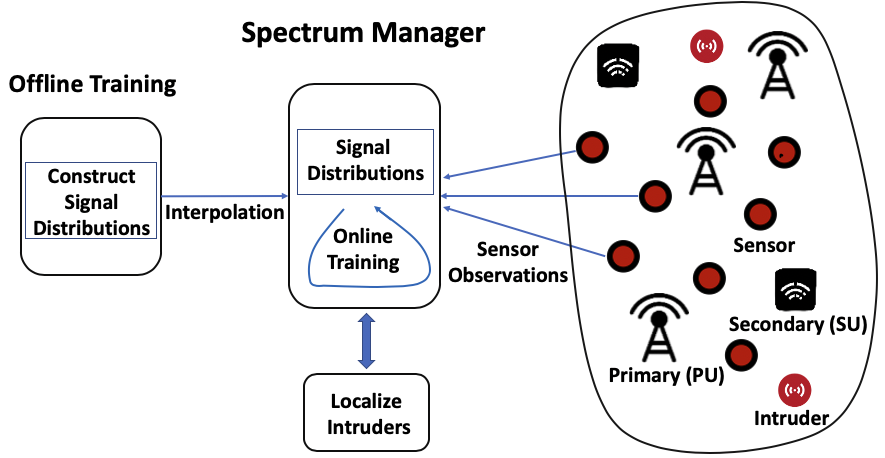
\includegraphics[width=0.95\textwidth]{chapters/ipsn/figures/architecture.png}
\caption{Overall approach to localize intruders in a shared spectrum system.} 
\label{fig:illustration}
\end{figure}

The increasing affordability of the software-defined radio (SDR)
technologies makes the shared spectrums particularly prone to
unauthorized usage or security attacks. With easy access to SDR
devices~\cite{usrp,hackrf}, it is easy for selfish users to transmit data
on shared spectrum without any authorization and potentially causing
harmful interference to the incumbent users.  Such illegal spectrum
usage could also happen as a result of infiltration of computer virus
or malware on SDR devices.  As the fundamental objective behind such
shared spectrum paradigms is to maximize spectrum utilization, the
viability of such systems depends on the ability to effectively guard
the shared spectrum against unauthorized usage.  The current
mechanisms however to locate such unauthorized users (intruders) are
human-intensive and time-consuming, involving FCC enforcement bureau
which detects violations via complaints and manual
investigation~\cite{mobicom17-splot}. 
\eat{As explained below, an effective
technique should be able to accurately localize multiple simultaneous
intruders and even in the presence of dynamically changing set of
authorized users.}
Motivated by above, we seek for an effective
technique that is able to accurately localize multiple simultaneous
intruders and even in the presence of dynamically changing set of
authorized users. In the following, we begin with describing the multiple transmitter localization problem.


%%% Multi-tx and challenges.
\para{Multiple-Transmitter Localization (MTL).}  \eat{Localization of
unauthorized users in a shared spectrum system essentially boils down to localizing transmitters/intruders in a given area under a shared spectrum system.}
 The transmitter localization problem has been well-studied, but most of the focus has been on localizing a {\em single} intruder at a time. However, it is important to localize multiple transmitters simultaneously to effectively guard a shared spectrum
system. E.g., a malware or virus-based attachment could simultaneously cause many devices to violate spectrum allocation rules; spectrum
jamming attacks would typically involve multiple transmitters. More
importantly, a technique limited by localization of a single intruder
could then be easily circumvented by an offender by using multiple
devices.
The key challenge in solving the MTL problem comes from the fact that
the deployed sensor would receive only a sum of the signals from multiple transmitters, and separating the signals may be impossible.  In
addition, the other challenge that MTL in the context of shared
spectrum system poses is the presence of authorized users---e.g., the
incumbent users and the dynamic set of secondary users that have been
allocated spectrum by the manager. To the best our knowledge, no prior
localization work has considered the presence of authorized users.

%%%% SPLOT and shortcomings.
The state-of-the-art technique for the MTL problem is the recent
work~\cite{mobicom17-splot}, which essentially decomposes the MTL
problem to multiple single-transmitter localization problems based on
the sensors with the highest power readings in a
neighborhood. \eat{To the best of our knowledge, this is the only
  work that has addressed the MTL problem extensively, especially in
  the context of shared spectrum systems.} However, the technique has
a few shortcomings: (i) it implicitly assumes a propagation model, and
thus, may not work effectively in areas with complex propagation
characteristics, (ii) it is not effective in the case of transmitters
being located close-by (a key challenging scenario for MTL problem),
and (iii) most importantly, it can't be extended effectively to
incorporate background authorized users, a key requirement in the
context of shared spectrum systems. 
\eat{In our evaluation, we
  have compared our technique with theirs and one other approach.}
%%\blue{Our localization approach belongs to the fingerprinting~\cite{infocom00-radar} category.}

%%%%%%%W WHAT we DO.
\para{Our Approach.}  Transmitter localization is generally done based
on observations at deployed sensors. In particular, as in prior
works~\cite{mobicom17-splot,chakraborty2017specsense}, we assume a
crowdsourced sensing architecture wherein relatively low-cost spectrum
sensors are available for gathering signal strength in the form of
received power. Our approach is a hypothesis-driven Bayesian approach,
viz.\ {\em maximum a posteriori} (\map) approach, wherein each
hypothesis is a configuration (i.e.  a combination of $\langle
location, power \rangle$ pair) of the potential intruders, and the
goal is to determine the hypothesis that best explains the sensor
observations. This determination is done based on the distributions
(gathered during a training phase) of sensor observations for each
hypothesis.
%%%%%%%%%%%%


%%%%% MOTIVATION.
\softpara{Motivation for \map.}  Our motivation for using a \map-based
approach is multifold: First, with sufficient training data, \map is
known to deliver optimal classification accuracy for the MTL problem.
Second, the \map approach doesn't assume any propagation model and
thus works for arbitrary signal propagation characteristics. Third, it
allows us to also estimate the intruder's transmit power, which can be
very useful in some applications, e.g., where the penalty is
proportional to the extent of violation. Lastly and most importantly,
it naturally extends to being able to handle a presence of an evolving
set of authorized users.

\softpara{Optimization and Novel Interpolation.} 
The benefits of a \mtl-based approach come at a cost. It
(i) incurs prohibitive computation cost---exponential in number of
potential intruders---when applied to the \mtl problem, and (ii)
requires significant amount of training cost. The focus of our work is
to address these challenges, and design a viable \map-based approach.

\emph{Optimization}. Using \map as a building block, we develop an optimized
approach that runs in polynomial time with minimized training cost using a divide-and-conquer idea.
We extend our technique to work in presence of authorized users by
incorporating online (real-time) training, which is enabled by utilizing some wireless signal charecteristics and thus incurs minimal cost.
\eat{We note that the online training to incorporate presence of authorized users is needed only for the prevailing setting (of authorized transmitters and deployed sensors) and hence incurs minimal cost
(see~\S\ref{sec:auth}). }

\blue{\emph{Novel Interpolation}. The \map framework requires prior
training to build probability distributions (PDs) of sensor
observations for each hypothesis.
In our work, we reduce the number of PDs to be constructed via a novel
interpolation scheme suited to our unique setting, and evaluate the
impact of reduced training on the localization accuracy.}

\para{Overall Contributions.}  The goal of our work is to develop an
efficient technique for accurate localization of simultaneously
present multiple intruders in a shared spectrum system. In this
context, we make the following specific contributions. 
\begin{enumerate}
\item
Design an efficient localization algorithm, i.e. \ouralgo, for the MTL problem, based
on an optimal hypotheses-driven Bayesian approach. The designed
approach predicts locations and transmit powers of the intruders, and
does not assume any propagation model and thus, works for arbitrary
signal propagation characteristics.

\item
Extend the designed algorithm to \ouralgoss, to localize effectively in the presence
of background authorized users, i.e., primaries with possibly unknown
parameters (e.g., location and transmit power) and an evolving set of
secondary users.

\item
Develop an effective interpolation scheme, i.e. \ildw, for our unique setting to
reduce the one-time training cost of our scheme, without impacting the
localization accuracy much.

\item
Evaluate our techniques via large-scale simulations as well as over
two developed testbeds (indoor and outdoor), and demonstrate the
effectiveness of our developed techniques and their superior
performance compared to the best-known techniques.
\end{enumerate}

%% We assume a crowdsourced architecture~\cite{}, wherein spectrum
%% sensing is delegated to independently deployed low-cost spectrum
%% sensors, such as rtl-sdr, who is merely over 20 dollars \cite{}.
%% Also there is a cloud-based spectrum manager~\cite{}, which 
%% orchestrates allocation of spectrum in such shared spectrum systems, 
%% based on available parameters and known channel conditions. 

%% The crowdsourcing spectrum sensor system scales well and realizes a
%% widespread and very cost-effective deployment.  Furthermore, it
%% facilitates the core spectrum management task we target at: guarding
%% the spectrum from unauthorized users.

%% Due to privacy, bandwith, and
%% cost concerns, it is impractical for the cheap sensors to send the
%% large raw signal I/Q samples to the cloud server.  Thus received
%% signal strength (RSS) is our choice of signal metrics.  So the sensors
%% process the raw signal I/Q samples locally and get RSS values, then
%% send the RSS values to the cloud.  Offloading the computation of
%% processing raw signal samples to the edge significantly decrease the
%% communication cost and enhance privacy.  T

% The best approach to date is \splot \cite{mobicom17-splot}, which utilized matrix inversion (essentially a variant of ridge regression) as a building block. However, it has an array of drawbacks. 
%% First and foremost, it is unable to localize two or more transmitters close by. 
%% The sensors' received signal is a phasor sum of the signals of both and \splot will report only one transmitter in the local maximum confined area.
%% Second, although it predicts location, it cannot predict the power of the transmitter. \splot is returning the coefficients of the ridge regression like function. 
%% The coefficients are correlated to the real power, but power is definitely not a function of those coefficients.
%% Third, the intrinsic mechanism of \splot assumes a propagation model.
%% They use a log normal model with an exponent of 2. However, the real environment may be more complicated than an ideal model, i.e. terrains can block and/or create multi-path reflection on the crowdsourced sensors.

%% The above three drawbacks comes from the settings of localizing only multiple illegal transmitters.
%% A fourth drawback will arise in the emerging shared spectrum system, where background transmissions from authorized users and potentially unauthorized offenders mixes together makes the proEvaluate our techniques via large-scale simulations as well as over
%two developed testbeds (indoor and outdoor), and demonstrate the
%effectiveness of our developed techniques and their superior
%performance compared to the best known techniques.blem harder by largely increasing the number of transmitters that need to be localized.
%% Multiple transmitter localization will hardly be perfect.
%% The more transmitters that need to localize, the less accuracy it gets.
%% For \splot, we see no good way of utilizing the information of authorized users to facilitate the localization of unauthorized offenders.
%% The way for \splot to work in a shared spectrum settings is to blindly localize all the transmitters and remove the known authorized users, then remains the unauthorized ones.
%% With this strategy, a smart spectrum offender can move close to an authorized user and safely transmit. 
%% \ble{In the mobicom-17 paper, they have a paragraph for dynamic localization, we might need to talk about it. It is a little related to our changing secondaries setting.}x

\chapter{Efficient Localization of Multiple Intruders for Shared Spectrum System}
\label{chap:ipsn}

% Abstract

We address the problem of localizing multiple intruders (unauthorized
transmitters) using a distributed set of sensors in the context of a
shared spectrum system. 
In contrast to single transmitter localization, multiple
transmitter localization (\mtl) has not been thoroughly studied.
In shared spectrum systems, it is important to be able to
localize simultaneously present multiple intruders to effectively
protect a shared spectrum from malware-based, jamming, or other
multi-device unauthorized-usage attacks. The key challenge in solving
the MTL problem comes from the need to ``separate'' an aggregated
signal received from multiple intruders into separate
signals from individual intruders. Furthermore, in a shared spectrum
paradigm, presence of an evolving set of authorized users (e.g.,
primary and secondary users) adds to the challenge.

In this paper, we propose an efficient algorithm for the \mtl problem
based on the hypothesis-based Bayesian approach called
\map. Direct application of the \map approach to
the \mtl problem incurs prohibitive computational and training
cost. In this work, we develop optimized techniques based on \map with
significantly improved computational and training costs. In
particular, we develop a novel interpolation method, \ildw, which helps
minimize the training cost. We generalize our techniques via
online-learning to the setting wherein there may be a set of
dynamically-changing authorized users present in the background.
We evaluate our developed techniques on large-scale simulations as
well as on small-scale indoor and outdoor testbeds. Our experiments
demonstrate that our technique outperforms the prior approaches by
significant margins,  i.e., error up to 74\% less in large-scale simulations and 30\% less in real-world testbeds.


\section{Introduction}
\label{sec:ipsn-intro}

The RF spectrum is a natural resource in great demand due to the
unabated increase in mobile (and hence, wireless) data
consumption~\cite{Jeffrey14}.  The research community has
addressed this capacity crunch via development of {\em shared spectrum
  paradigms}, wherein the spectrum is made available to unlicensed
users (secondaries) as long as they do not interfere with the
transmission of licensed incumbents (primaries).  E.g., in the recent
years, the FCC has made available the CBRS band, i.e., the 3550-3700
MHz band within the 3.5 GHz band, for shared commercial use to allow
other users to utilize the otherwise low-usage band which was
previously reserved for incumbent users including US Navy radar
operators.


\begin{figure}[t]
\centering
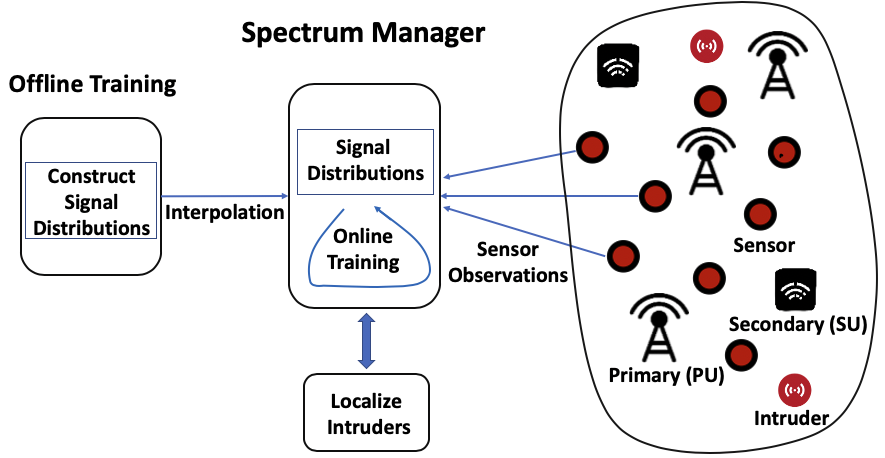
\includegraphics[width=0.95\textwidth]{chapters/ipsn/figures/architecture.png}
\caption{Overall approach to localize intruders in a shared spectrum system.} 
\label{fig:ipsn-illustration}
\end{figure}

The increasing affordability of the software-defined radio (SDR)
technologies makes the shared spectrums particularly prone to
unauthorized usage or security attacks. With easy access to SDR
devices~\cite{usrp,hackrf}, it is easy for selfish users to transmit data
on shared spectrum without any authorization and potentially causing
harmful interference to the incumbent users.  Such illegal spectrum
usage could also happen as a result of infiltration of computer virus
or malware on SDR devices.  As the fundamental objective behind such
shared spectrum paradigms is to maximize spectrum utilization, the
viability of such systems depends on the ability to effectively guard
the shared spectrum against unauthorized usage.  The current
mechanisms however to locate such unauthorized users (intruders) are
human-intensive and time-consuming, involving FCC enforcement bureau
which detects violations via complaints and manual
investigation~\cite{mobicom17-splot}. 
\eat{As explained below, an effective
technique should be able to accurately localize multiple simultaneous
intruders and even in the presence of dynamically changing set of
authorized users.}
Motivated by above, we seek for an effective
technique that is able to accurately localize multiple simultaneous
intruders and even in the presence of dynamically changing set of
authorized users. In the following, we begin with describing the multiple transmitter localization problem.


%%% Multi-tx and challenges.
\para{Multiple-Transmitter Localization (MTL).}  \eat{Localization of
unauthorized users in a shared spectrum system essentially boils down to localizing transmitters/intruders in a given area under a shared spectrum system.}
 The transmitter localization problem has been well-studied, but most of the focus has been on localizing a {\em single} intruder at a time. However, it is important to localize {\em multiple} transmitters {\em simultaneously} to effectively guard a shared spectrum
system. E.g., a malware or virus-based attachment could simultaneously cause many devices to violate spectrum allocation rules; spectrum
jamming attacks would typically involve multiple transmitters. More
importantly, a technique limited by localization of a single intruder
could then be easily circumvented by an offender by using multiple
devices.
The key challenge in solving the MTL problem comes from the fact that
the deployed sensor would receive only a sum of the signals from multiple transmitters, and separating the signals may be impossible.  In
addition, the other challenge that MTL in the context of shared
spectrum system poses is the presence of authorized users---e.g., the
incumbent users and the dynamic set of secondary users that have been
allocated spectrum by the manager. To the best our knowledge, no prior
localization work has considered the presence of authorized users.

%%%% SPLOT and shortcomings.
The state-of-the-art technique for the MTL problem is the recent
work~\cite{mobicom17-splot}, which essentially decomposes the MTL
problem to multiple single-transmitter localization problems based on
the sensors with the highest power readings in a
neighborhood. \eat{To the best of our knowledge, this is the only
  work that has addressed the MTL problem extensively, especially in
  the context of shared spectrum systems.} However, the technique has
a few shortcomings: (i) it implicitly assumes a propagation model, and
thus, may not work effectively in areas with complex propagation
characteristics, (ii) it is not effective in the case of transmitters
being located close-by, a key challenging scenario for MTL problem,
and (iii) most importantly, it can't be extended effectively to
incorporate background authorized users, a key requirement in the
context of shared spectrum systems. 
\eat{In our evaluation, we
  have compared our technique with theirs and one other approach.}
%%\blue{Our localization approach belongs to the fingerprinting~\cite{infocom00-radar} category.}

%%%%%%%W WHAT we DO.
\para{Our Approach.}  Transmitter localization is generally done based
on observations at deployed sensors. In particular, as in prior
works~\cite{mobicom17-splot,chakraborty2017specsense}, we assume a
crowdsourced sensing architecture wherein relatively low-cost spectrum
sensors are available for gathering signal strength in the form of
received power. Our approach is a hypothesis-driven Bayesian approach,
viz.\ {\em maximum a posteriori} (\map) approach, wherein each
hypothesis is a configuration (i.e.  a combination of $\langle
location, power \rangle$ pair) of the potential intruders, and the
goal is to determine the hypothesis that best explains the sensor
observations. This determination is done based on the distributions
(gathered during a training phase) of sensor observations for each
hypothesis.
%%%%%%%%%%%%
The \map approach is known to have optimal classification accuracy,
but (i) incurs prohibitive computation cost---exponential in number of
potential intruders---when applied to the \mtl problem, and (ii)
requires significant amount of training cost. The focus of our work is
to address these challenges, and design a viable \map-based approach.
%%%
In particular, using \map as a building block, we develop an optimized
approach that runs in polynomial time with minimized training cost.
We extend our technique to work in presence of authorized users by
incorporating online (real-time) training.

%%%%% MOTIVATION.
\softpara{Motivation for \map.}  Our motivation for using a \map-based
approach is multifold: First, with sufficient training data, \map is
known to deliver optimal classification accuracy for the MTL problem~\cite{map-optimal}.
Second, the \map approach doesn't assume any propagation model and
thus works for arbitrary signal propagation characteristics. Third, it
allows us to also estimate the intruder's transmit power, which can be
very useful in some applications, e.g., where the penalty is
proportional to the extent of violation. Last but not the least,
it naturally extends to being able to handle a presence of an evolving
set of authorized users.

\softpara{Training Cost and Optimization.}  The benefits of a \map-based
approach come at a cost: the \map framework requires prior training to
build probability distributions (PDs) of sensor observations for each
hypothesis. However, most of the training occurs offline, one-time,
and can be automated e.g.\ via drones or robots.  In our work, we
develop strategies to minimize the training cost; in particular, we
reduce the number of PDs to be constructed via a {\em novel interpolation
scheme} suited to our unique setting, and evaluate the impact of
reduced training on the localization accuracy.
%%%
We note that the online training to incorporate presence of authorized
users is needed only for the prevailing setting (of authorized
transmitters and deployed sensors) and hence incurs minimal cost
(see~\S\ref{sec:auth}).

\para{Overall Contributions.}  The goal of our work is to develop an
efficient technique for accurate localization of simultaneously
present multiple intruders in a shared spectrum system. The raw data are available at https://github.com/Wings-Lab/IPSN-2020-data. In this
context, we make the following four specific contributions. 
\begin{enumerate}
\item
Design an efficient localization algorithm (\ouralgo) for the MTL
problem, based on an optimal hypotheses-driven Bayesian approach. The
designed approach predicts both locations and transmit powers of the
intruders, and does not assume any propagation model and thus, works
for arbitrary signal propagation characteristics.

\item
Extend the designed algorithm (\ouralgoss) to localize effectively in
the presence of background authorized users, i.e., primaries with
possibly unknown parameters (e.g., location and transmit power) and an
evolving set of secondary users.

\item
Develop an effective interpolation scheme (\ildw) for our unique
setting to reduce the one-time training cost of our scheme, without
impacting the localization accuracy much.

\item
Evaluate our techniques via large-scale simulations as well as over
two developed testbeds (indoor and outdoor), and demonstrate the
effectiveness of our developed techniques and their superior
performance compared to the best-known techniques.
\end{enumerate}

%% We assume a crowdsourced architecture~\cite{}, wherein spectrum
%% sensing is delegated to independently deployed low-cost spectrum
%% sensors, such as rtl-sdr, who is merely over 20 dollars \cite{}.
%% Also there is a cloud-based spectrum manager~\cite{}, which 
%% orchestrates allocation of spectrum in such shared spectrum systems, 
%% based on available parameters and known channel conditions. 

%% The crowdsourcing spectrum sensor system scales well and realizes a
%% widespread and very cost-effective deployment.  Furthermore, it
%% facilitates the core spectrum management task we target at: guarding
%% the spectrum from unauthorized users.

%% Due to privacy, bandwith, and
%% cost concerns, it is impractical for the cheap sensors to send the
%% large raw signal I/Q samples to the cloud server.  Thus received
%% signal strength (RSS) is our choice of signal metrics.  So the sensors
%% process the raw signal I/Q samples locally and get RSS values, then
%% send the RSS values to the cloud.  Offloading the computation of
%% processing raw signal samples to the edge significantly decrease the
%% communication cost and enhance privacy.  T









% The best approach to date is \splot \cite{mobicom17-splot}, which utilized matrix inversion (essentially a variant of ridge regression) as a building block. However, it has an array of drawbacks. 
%% First and foremost, it is unable to localize two or more transmitters close by. 
%% The sensors' received signal is a phasor sum of the signals of both and \splot will report only one transmitter in the local maximum confined area.
%% Second, although it predicts location, it cannot predict the power of the transmitter. \splot is returning the coefficients of the ridge regression like function. 
%% The coefficients are correlated to the real power, but power is definitely not a function of those coefficients.
%% Third, the intrinsic mechanism of \splot assumes a propagation model.
%% They use a log normal model with an exponent of 2. However, the real environment may be more complicated than an ideal model, i.e. terrains can block and/or create multi-path reflection on the crowdsourced sensors.

%% The above three drawbacks comes from the settings of localizing only multiple illegal transmitters.
%% A fourth drawback will arise in the emerging shared spectrum system, where background transmissions from authorized users and potentially unauthorized offenders mixes together makes the proEvaluate our techniques via large-scale simulations as well as over
%two developed testbeds (indoor and outdoor), and demonstrate the
%effectiveness of our developed techniques and their superior
%performance compared to the best known techniques.blem harder by largely increasing the number of transmitters that need to be localized.
%% Multiple transmitter localization will hardly be perfect.
%% The more transmitters that need to localize, the less accuracy it gets.
%% For \splot, we see no good way of utilizing the information of authorized users to facilitate the localization of unauthorized offenders.
%% The way for \splot to work in a shared spectrum settings is to blindly localize all the transmitters and remove the known authorized users, then remains the unauthorized ones.
%% With this strategy, a smart spectrum offender can move close to an authorized user and safely transmit. 
%% \ble{In the mobicom-17 paper, they have a paragraph for dynamic localization, we might need to talk about it. It is a little related to our changing secondaries setting.}x

\section{Problem, Related Work, and Methodology}
\label{sec:ipsn-problem}

In this section, we describe our model of the shared spectrum systems,
formulate the \mtl problem, and discuss related work.  We also
describe the building block of our approach, viz., a hypothesis-driven
Bayesian localization approach (\map).

\para{Shared Spectrum System.} In a shared spectrum paradigm, the
spectrum is shared among licensed users (primary users, PUs) and
unlicensed users (secondary users, SUs) in such a way that the
transmission from secondaries does not interfere with that of the
primaries (or secondaries from a higher-tier, in case of a multi-tier
shared spectrum system~\cite{scte-isbe16-cbrs}). In some shared spectrum systems,
the location and transmit power of the primary users may be
unavailable, as is the case with military or navy radars in the CBRS
band~\cite{scte-isbe16-cbrs}.
%%%%%
Such sharing of spectrum is generally orchestrated by a centralized
entity called {\em spectrum manager}, such as a spectrum
database in TV white
space~\cite{sas-paper} or a central spectrum access system in
the CBRS 3.5GHz shared band~\cite{milind2015dyspan}. The spectrum
manager allocates spectrum to requesting secondaries (i.e., permission
to transmit up to a certain transmit power at their location) based on
their location, spectrum demand, configurations of the primaries, other
active secondaries, prevailing channel conditions, etc.
SwarmShare~\cite{jiangqi2021spectrum,jiangqi2023spectrum} is proposed to enable spectrum sharing
between the incumbent systems and the coexisting UAV networks in the 6GHz band.
Researchers have developed NeXT~\cite{jiangqi2022next,jiangqi2023next}, a software-defined wireless testbed, 
to support both traditional model-based control and new data-driven control techniques in wireless research.

\para{Authorized and Unauthorized Users.}
Secondary users that have been explicitly given permission to transmit
at their location are termed as {\em authorized users}; the primary
users are also considered as authorized users. Note that the set of
authorized users evolve over time, as more and more SUs are allocated
spectrum and as some SUs stop using the spectrum after a while. We can
assume that each SU is allocated spectrum for a certain duration of
time, after which it stops using the spectrum. 
%%%%%%%%%%%%
Other users that transmit without explicit permission (for that given
time) are referred to as {\em unauthorized users} or {\em intruders}.

\para{Problem Setting and Formal Definition.}  Consider a geographic
area with a shared spectrum. Without loss of generality, we assume a
single channel throughout this paper (multiple channels are handled
similarly). For localization of unauthorized users, we assume
available crowdsourced sensors that can observe the received signal in the
channel of interest, and compute (total) received signal strength
indicator (RSSI)\footnote{We do not use angle-of-arrival (AoA)
    measurements~\cite{aoa-multi} as they require additional and
    complex RF hardware.}. These sensors, being crowdsourced, may be at
  different locations at different times.  At any given instant, the
  shared spectrum area has some licensed primary users and some active
  secondary users; the PU configurations may not be known as can be
  the case for military users. The centralized spectrum manager is
  aware of the set of active SUs at any time, as each SU request is
  granted for a certain period of time.
%%%%
In addition to the authorized users, there may be a set of intruders
present in the area with each intruder in a certain ``configuration''
(see \S\ref{sec:map}).

The \mtl problem is to determine the set of intruders with their
configurations at each instant of time, based on the set of sensor
observations at that instant. See Figure \ref{fig:ipsn-illustration}. 
The basic \mtl problem assumes no other
transmissions (of authorized users) in the background.
%%%%%
The more general \mtl problem, where there may be an evolving set of
authorized users in the background, is referred to as the \mtlss
problem.  We address the \mtl problem in~\S\ref{sec:map-time}, and
then address the more general \mtlss problem in~\S\ref{sec:mtlss}.

%% Let $\theta_i = (l_i, p_i)$ denotes the configuration of location and
%% power of one transmitter, and $\boldsymbol{\theta_M} = \{\theta_1,
%% \theta_2, \cdots, \theta_M \}$ denotes the configurations of all
%% intruders. 
%% The problem is to predict $\boldsymbol{\theta_M}$ based on the observed received power
%% reported by sensor $\vx = \{x_1, x_2, \cdots, \}$.

\subsection{Related Work}
\label{sec:ipsn-related}

Localization of an intruder in a field using sensor observations has
been widely studied, but most of the works have focused on
localization of a single intruder~\cite{infocom18-spectrum,dutta2016see}.
%%%%%
In general, to localize multiple intruders, the main challenge comes
from the need to ``separate'' powers at the sensors~\cite{mobicom-30},
i.e., to divide the total received power into power received from
individual intruders. Blind source separation is a very challenging
problem; only very limited settings allow for known
techniques~\cite{freq-sig,ben-zhao} using sophisticated receivers. In
our context of hypotheses-driven approach, the challenge of source
separation manifests in terms of a large number of hypotheses, a
challenge addressed in~\S\ref{sec:map-time}.
%%%
We note that (indoor) localization of a
  device~\cite{infocom00-radar} based on signals received from multiple reference points (e.g, WiFi access
  points) is a quite different problem
  (see~\cite{zafari-19} for a recent survey), as the signals from
  reference points remain separate, and localization or tracking of multiple
  devices can be done independently.
  Recent works on multi-target localization/tracking are different in the way that targets are passive~\cite{ipsn19-multipassive, ipsn19-chorus, ipsn19-snaploc}, instead of active transmitters in this work.

In absence of blind separation methods, to the best of our knowledge,
only a few works have addressed multiple intruder(s) localization, and
none of these consider it in the presence of a dynamically changing
set of authorized transmitters. In particular,
(i)~\cite{mobicom17-splot} decomposes the multi-transmitter
localization problem to multiple single-transmitter localization
problems based on the sensors with highest of readings in a
neighbohood, (ii)~\cite{clustering} works by clustering the sensors
with readings above a certain threshold and then localizing intruders
at the centers of these clusters, (iii)~\cite{Quasi-EM} uses an
EM-based approach.
%%%
The techniques of~\cite{mobicom17-splot,Quasi-EM} assume a propagation
model, while that of~\cite{clustering,Quasi-EM} require a priori
knowledge of the number of intruders present.  We have compared our
approach with~\cite{mobicom17-splot,clustering} in \S\ref{sec:eval},
while~\cite{Quasi-EM} has high computational cost and has also been
shown to be inferior in performance
to~\cite{mobicom17-splot,clustering} even for a small number of
intruders. Other related works include
  (i)~\cite{multi-tx-dyspan-19} that addresses the challenge of
  handling time-skewed sensors observations in the MTL problem, and
  (ii)~\cite{info-20} that addresses the sensor selection optimization
  problem for our proposed hypotheses-based localization approach.
  
%%%%%
%\blue{Other related works include:~\cite{mobicom-22} where sensors are
%  on mobile and controlled robots,~\cite{mobi-25} focusses on spectrum
%  allocation via spectrum hole detection in presence of background 
%  transmitters.} \red{HG: Remove this sentence?}

%% Online selection of sensors: ipsn-04, .... latency vs. energy .. since,
%% latency is equally critical, ... we dont want to run it for every intruder ... 
%% Similarly,
%% \cite{krause2008near} shows that minimizing uncertainty in a gaussian
%% process is submodular, and thus greedy selection provides a bounded
%% solution to the optimal.

%% Multiple studies have studied sensor selection to maximize the
%% accuracy of detection of some event \cite{rowaihy2007survey}.

%% For
%% example, \cite{joshi2009sensor} provides a heuristic for sensor
%% selection by forming a convex optimization problem.  However, it uses
%% a different metric to measure the accuracy of detection.
%% %%%%
%% Other studies, such as
%% \cite{shamaiah2010greedy} and \cite{bian2006utility} have proposed
%% leveraging submodularity to select sensors.  

%% There are also studies in the active learning literature that focus on
%% online selection.  For example, \cite{yuxin-when} limits the mutual
%% information while selecting the minimum possible number of sensors.
%% \cite{krause2012near} shows that mutual information in sensor
%% selection is submodular in the absence of noise and propose a
%% probabilistic greedy algorithm by leveraging it.
%% \cite{golovin2011adaptive} proposes the concept of adaptive
%% submodularity that generalizes the greedy approximation to online
%% selection. Our online selection algorithm builds upon these studies to
%% limit the number of sensors while maximizing the mutual information.
%% However, in the presence of noise, mutual information is not adaptive
%% submodular in nature.  Thus, our work modifies the algorithm discussed
%% in \cite{yuxin-when} to make it suitable for our use case.


\subsection{\map: Bayesian Approach for Localization}
\label{sec:map}

We localize intruders based on observations from a set of
sensors. Each sensor communicates its observation to a centralized
entity, the spectrum manager, which runs an appropriate
localization algorithm to localize the intruders.
%%%%
In particular, we use a hypotheses-driven Bayesian approach, as
described below, where intruders are localized by determining the
most likely prevailing hypothesis; this is done based on joint
probability distributions of the sensors' observations (constructed
during a priori training). Below, we formalize the above concepts, and
the basic localization approach.

\para{Observation; Observation Vector.} Throughout this
paper, we use the term {\em observation} at an individual sensor to
mean the received power over a time window of certain duration, in the
frequency channel of interest (we assume only one channel). In
particular, received power is computed from the FFT of the I/Q samples
in the time window~\cite{arani2018}. We use the term {\em observation
  vector} \vx to denote a vector of observations from a given set of
distributed sensors, with each vector dimension corresponding to a
unique sensor.
%%%%%%%%
%% We assume a Gaussian distribution $N (\mu, \sigma^2)$ for each
%% observation, where mean implies the average power the receiver
%% receive, and standard deviation will represent the noise, shadowing,
%% and multi-path fading.

\begin{wrapfigure}{r}{2in}
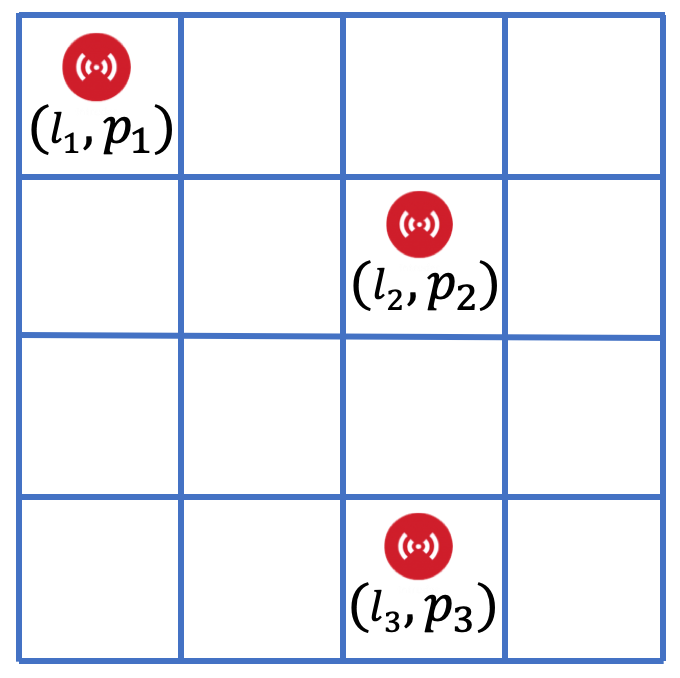
\includegraphics[width=2in]{chapters/ipsn/figures/hypothesis.png}
\caption{Illustration of a hypothesis formed of three transmitters.}
\label{fig:hypothesis-grid}
\end{wrapfigure}
\para{Hypotheses.} Let \hz, \ho, $\ldots,$ \hM be the set of all
hypotheses, where each hypothesis \hj represents a ``configuration''
of potential intruders. In this chapter, we largely assume an
  intruder's configuration to be comprised of just its location and
  transmit power, but the concept of configuration is quite general
  and could include any attributes (e.g., height, antenna direction,
  etc.) that affect how its transmitted signal is received at other
  locations. Moreover, for simplicity, we assume that each intruder
  transmits at a fixed power (which may be different for different
  intruders). Thus, in our context, a configuration is simply the set
of (location, transmit power) pairs of potential intruders. We
assume a bounded number of intruders. We use \hz to represent the
hypothesis with no intruders. See Figure~\ref{fig:hypothesis-grid}.

%%%%%%%
If there is only one intruder, then each hypothesis represents the
location and transmit power combination of the intruder, and
determining the hypothesis is equivalent to localizing the intruder
and estimating its power. If we allow multiple intruders at a time,
the number of possible hypotheses can be exponential in the number of
intruders; we will address this challenge in
\S\ref{sec:map-time}.

\softpara{Inputs.} For a given set of sensors deployed over an area, we
assume the following available inputs, obtained via a priori training,
data gathering and/or analysis:
\begin{itemize}
\item
Prior probabilities of the hypotheses, i.e. $P(H_i)$, for each
hypothesis $H_i$. Prior probabilities come from known knowledge about
the area, intruder's behavior, etc., and can be assumed to be uniform in
absence of better knowledge.

\item
Joint probability distribution (JPD) of sensors' observations for each
hypothesis. More formally, for each hypothesis $H_j$, we assume
$P(\vx|H_j)$ to be known for each observation $\vx$ for the set of
deployed sensors.  The JPDs can be obtained from prior training, a
combination of training and interpolation (\S\ref{sec:inter}), or
even by assuming a propagation model to remove the training
cost completely.
\end{itemize}

\para{Maximum a Posteriori (\mll) Localization Algorithm.}  We use
Bayes rule to compute the likelihood probability of each hypothesis,
from a given observation vector $\vx$:
\begin{equation}
  P(H_i | \vx) = \frac{P(\vx| H_i)P(H_i)}{\sum_{j=0}^m P(\vx|H_j)P(H_j)}
  \label{eqn:bayes}
\end{equation}
We select the hypothesis that has the highest probability, for given
observations of a set of sensors. That is, the \mll Algorithm returns
the hypotheses based on the following equation:
\begin{equation}
  \arg \max_{i=0}^m P(H_i | \vx)
  \label{eqn:map}
\end{equation}
The above \mll algorithm to determine the prevailing hypothesis is
known to be {\em optimal}~\cite{map-optimal}, i.e., it yields the minimum
probability of (misclassification) error. The above hypothesis-based
approach to localization works for arbitrary signal propagation
characteristics, and in particular, obviates the need to assume a
propagation model. However, the above \mll algorithm does incur a {\em
  one-time} training cost to construct the JPDs.




\section{{\texorpdfstring{\ouralgo}: Optimizing \mll for MTL}}
\label{sec:map-time}

The \map algorithm of \S\ref{sec:map} can be directly applied to
localize multiple intruders with optimal localization accuracy.
However, \map incurs prohibitive computational costs, especially for a
large number of potential intruders.  In particular, note that if
there are $L$ potential locations, up to $T$ potential intruders, and
$W$ possible discrete transmit-power levels, then the
hypotheses-driven \map algorithm needs to consider $(LW)^T$
hypotheses---making its runtime complexity exponential in the number of
potential intruders, and thus, making it impractical to localize
even a moderate number of intruders present simultaneously.  In
addition, \mll also incurs a high training cost. In the following
subsections, we develop an optimized algorithm called \ouralgo based
on \map but with significantly improved computational and
training cost.
%%%%%
We start with optimizing the computation cost in \S\ref{sec:time}. In the following
  subsection \S\ref{sec:ipsn-power}, we derive a closed-form expression
  to efficiently estimate the intruder's power in the {\em continuous}
  domain.  Finally, we discuss optimizing the training cost via a
  novel interpolation scheme \ildw.

%% Next, we use this result to design a computationally
%% efficient algorithm in the following section
%% 2) optimizing the \map algorithm in a way that
%% minimizes the subarea where ``simultaneous'' localization of multiple
%% intruders needs to be considered (the source of exponential
%% complexity).  The former cancels $W$ in the base and the later reduces
%% $L$ in the base.

%\subsection{Intruder Power Estimation in the Continuous Domain}
\label{sec:ipsn-power}

In this subsection, we derive a {\em closed-form} expression to estimate an
intruder's power in the continuous domain, for the special case of
single intruder and Gaussian probability
distributions~\cite{gauss}. The derived result essentially removes the
assumption of discrete power levels, and reduces the number of
hypotheses to consider by a factor of $W$. We use
this result within Procedure~1 of the previous subsection to further
optimize its time complexity and performance.

\para{Estimating Intruder Power, Given a Location.}  Consider the
special case of a single intruder in an area. In this case, each
hypothesis can be represented as \hlp, for each location $l$ and power
$p$ of the potential intruder. Let us focus on a particular location
$\lstar$ and the corresponding hypotheses \hLp. 
%%%%%
For a given observation vector \vx, we wish to estimate the power $P$
that corresponds to the hypothesis with maximum likelihood among the
hypotheses \hLp.
$$P = \arg max_p P(\hLp | \vx)$$
%%%%
The value $P$ can be computed by computing $P(\hLp | \vx)$ for
each $p$, but our goal is to derive a closed-form expression for $P$
from the given JPDs; such an expression yields power estimate in
continuous domain without computing $P(\hLp | \vx)$ for each possible
discrete $p$.

For each sensor (location) $j$, let $\pd(\vx_j | \hLP)$ represent the
probability distribution (PD) of $j$'s observations $\vx_j$ when the
intruder is at \lstar transmitting with power \pstar, the power used
at training.
%%%%%%
For a fixed \lstar and \pstar, the set of PDs $\pd(\vx_j | \hLP)$ are
equivalent to the JPDs defined in \S\ref{sec:ipsn-problem} under the
assumption of conditional independence\footnote{PD $\pd(\vx_j |
  \hLp)$ can be computed $\pd(\vx_j | \hLP)$ for any $p$, as the
  path-loss can be assumed to be independent of the transmit power,
  and JPD $\pd(\vx | \hLp)$ can be computed as product of PDs
  $\pd(\vx_j | \hLp)$ due to the conditional independence assumption.}.
%%%%%%%
%%%%%%%%
Let us assume that the above PDs are Gaussian
distributions~\cite{gauss}, and thus, can be represented as $\pd(\vx_j
| \hLP) = N(\mu_j, \sigma_j^2)$ for a given $\lstar$ and $\pstar$.
%%%%%%%%%%%%%
In the above setting, the power value $P$ that maximizes $P(\hLp | \vx)$
can actually be derived as a closed-form expression; we state the result
formally in the below lemma. 
\begin{lemma-wo-prf}
  Consider the special case of a single intruder in an area.  For a
  specific location $\lstar$ and power $\pstar$ (the only power used
  during training), let $\pd(\vx_j | \hLP)$ represent the PDs of the
  sensor observations at location $j$. Now, given the above PDs for
  various $j$ and an observation vector $\vx$, the power value
  $P = \arg max_p P(\hLp | \vx)$ is   given by: 
  $$\pstar + \frac{\sum_{j=1}^{S} \frac{\gamma}{\sigma_j^2}(x_j - \mu_j)}{\sum_{j=1}^{S} \frac{\gamma}{\sigma_j^2}},$$
  where $\gamma = \prod_{j=1}^{S} \sigma_j^2$ and S equals the number of sensors in the neighborhood of  $\ \lstar$.
  \label{lem:p}
\end{lemma-wo-prf}
The proof is in Appendix~\ref{appen:ipsn}. 
Here, we give its intuition based on a special case. 
Consider the special case wherein each $\sigma_j$ is 1 for all
$j$. In this special case, the Lemma's equation reduces to $P = \pstar
+ \frac{\sum_{j=1}^{S}(x_j - \mu_j)}{|S|}$, which implies that if each
observation $x_j$ is $c$ more than its mean $\mu_j$ then $P$ is also
$c$ more than $\pstar$. We note that the above result does {\em not}
extend to the case of multiple intruders. In short, the proof is a process of solving maximum likelihood estimation and multiple intruders introduce transcendental functions, thus cannot derive a closed-form solution.

\para{Use of Lemma~\ref{lem:p} in \ouralgo.} \eat{First, we note that,
  for the special case of a single intruder, the result of
  Lemma~\ref{lem:p} essentially allows us to determine continuous
  power value of the intruder while also reducing the overall
  computational complexity of the optimal \mll algorithm by a factor
  of $W$, the number of discrete power levels.}  For localization of
multiple intruders, Lemma~\ref{lem:p} can only be used in Procedure~1
of \S\ref{sec:time}, due to its assumption of a single intruder. In
particular, we can Procedure~1 of \S\ref{sec:time} as follows.
\begin{itemize}
\item
We replace \Rp by $R$, the maximum transmission radius.
  
\item
For each location $l$, using Lemma~\ref{lem:p}, we first compute the
power $p(l)$ such that the hypothesis \hlpl has the most likelihood
(among the hypotheses at $l$) using the observations from sensors
within a radius of $R$.
\item
Then, in the rest of the procedure, we only consider the (location,
power) pairs of the type $(l, p(l))$ for any $l$.
\end{itemize}
The rest of the Procedure~1 remains unchanged. The above change has two
benefits. First, the powers predicted in Procedure~1 are now
continuous rather than discrete. Second, the above removes the factor
of $W$ from the time complexity of \ouralgo and reduces it to
$O(LG_R\log(G_R) + G_R(G_R)^T)$ which becomes $O(L)$ if we consider
$G_R$ and $T$ to be relatively small constants.


\subsection{Optimizing Computation Time}
\label{sec:time}

\para{Basic Idea.}  Note that the \mll's exponential time complexity
is due to the exponential number of {\em combinations} of locations
and/or powers of the potential intruders. To motivate our proposed
optimized approach, consider a simple example of 2 intruders with
fixed power $p$ in a large area. Assume that the ``transmission
radius'' $r$ for power $p$ is much smaller than the area; we define
the {\em transmission radius} as the range till which the received
signal is more than a certain noise floor.
%%%%
The key observation is that if the intruders are far away (isolated)
from each other (specifically, more than $2r$ distance away), then
they could be localized independently. If the intruders are closer,
then there is a need to separate aggregated signal at some of the
sensors and hence we must apply the standard \mll algorithm {\em
  within that ``subarea''}; however, since each such subarea is small
(a disk of $2r$ radius around each possible location), the computation
time is reduced significantly. However, since we do not a priori know
the configurations of intruders, we need to consider appropriate
possibilities.

In essence, our optimized approach is a divide-and-conquer approach,
consisting of a sequence of two procedures each of which is executed
iteratively. The first procedure focuses on localizing ``isolated''
intruders (if any) independently, while the second procedure localizes
the remaining intruders---by considering all possible subareas as
suggested above. The challenge lies in modifying the \mll algorithm
for each iteration of the above procedures---as the hypotheses to
consider across iterations of the procedures are not disjoint. We now
describe each of the procedures.

\para{Procedure 1. Localize Isolated Intruders.}  Informally, in this
procedure, we localize intruders that are sufficiently separated from
other intruders. In other words, we localize intruders $x$ that are
surrounded by sensors that receive most of their received power from
$x$. More formally, we localize an intruder $x$ at location $l$ if (i)
$l$'s ``neighborhood'' has at least 3 sensors that receive most of
their power from $x$, and (ii) there are no other intruders in the
``vicinity'' of $l$. In essence, we iterate over all locations $l$,
and localize an intruder at $l$ if the above conditions are satisfied
with high enough probability, based on the readings of sensors around
$l$.
%%%%%
The precise definition of neighborhood above must depend on $x$'s
transmission radius which depends on its transmit power; however, as
$x$'s transmit power is unknown, we iterate over smaller and smaller
neighborhoods.

We now formally describe the procedure.  Let \Rp denote the
transmission radius for a transmit power of $p$. Let $R$ denote the
maximum transmission radius, i.e., $$\max_p \Rp.$$ In the below
description, we use a fractional value $f$ to define a neighborhood
and vicinity size. We start $f$ equal to 1, use a disk of radius
$f\Rp$ as a neighborhood and $R + f\Rp$ as the vicinity, and iterate
over the procedure for reduced values of $f$.
\begin{packedalpha}
	\item
	Let $f$ = 1.
	
	\item
	For each location and power pair $(l,p)$, compute $P(\hlp |
        \vxlp)$ using a form of Equation~\ref{eqn:bayes} over
        appropriate JPDs. Here:
        \begin{itemize}
          \item
         \hlp represents the hypothesis that an intruder is at
         location $l$ and using $p$ transmit power. We also implicitly
         assume that there is no other intruder present within a
         distance of $R + f\Rp$ from $l$; this ensures that the
         observations in $\vxlp$ are only due to the intruder at $l$.
         See Figure ~\ref{fig:mmap}.
         
       \item
         $\vxlp$ represents the observation vector for all sensors,
         but the sensors that are within a radius of $f\Rp$ around
         $l$ use an observation of ``residual'' received powers, as
         defined below, while the remaining sensors (outside the
         radius of $f\Rp$ around $l$) use an observation of the
         ``noise floor'' (in essence, we are ``zeroing'' the
         observations of the far-away sensors). See Figure~\ref{fig:mmap}.
         \end{itemize}
	
	\item
	Denote $(l,p)$ pairs that have $P(\hlp | \vxlp)$ higher than a
        certain threshold as {\em peaks}. If a location $l$ is a peak
        and there are no other peaks within a distance of $R + f\Rp$,
        then {\bf localize an intruder at $l$ with transmit power
          $p$.}

      \item
	For each sensor $s$, define its {\em residual received power}
          (RRP) as the total received power reduced by the sum of
        mean powers received from already localized intruders; the
        desired mean values are available from the given
        JPDs.
	
	\item
	Reduce $f$ and go back to step \#2 above, unless no new
        intruders were localized in (c) above. In our experiments, we
        used $f = 1, 1/2, 1/4$ and $1/8$.
\end{packedalpha}

\begin{figure}
	\centering
	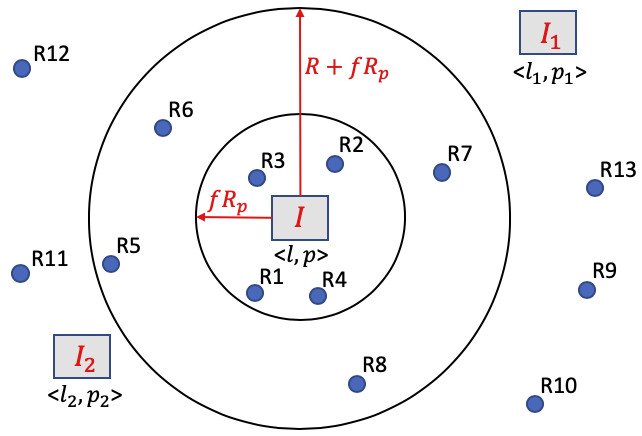
\includegraphics[width=0.7\textwidth]{chapters/ipsn/figures/mmap.png}
	\caption{Illustration of Hypothesis \hlp in Step (b) of
          Procedure~1. Here, the intruder $I$ at location $l$ is
          transmitting at power $p$, with no other intruder within a
          distance of $R + f\Rp$ from $I$. The observation vector
          $\vxlp$ consists of residual received powers from $R1$ to
          $R4$, and ``noise floor'' from the remaining sensors.}
	\label{fig:mmap}
\end{figure}

The above procedure is partly inspired by the recent localization
work~\cite{clustering}. However, instead of discarding sensors based
on their individual power and clustering the rest as
in~\cite{clustering}, we ``discard'' sensors based on their
neighborhood readings (i.e., likelihood $P(\vx| H_i)$ values) and then
``cluster'' the remaining sensors. Also, we ``cluster'' iteratively,
for smaller and smaller neighborhoods.

%% Our above procedure is partially inspired by the recent localization
%% work~\cite{clustering}, which discards sensors that receive power
%% below a certain threshold, clusters the remaining sensors, and then
%% place an intruder in each cluster. In effect, we ``discard'' a sensor
%% $s$ based on information from $s$'s neighborhood (i.e., likelihood P()
%% values) rather than $s$'s individual power as in~\cite{clustering}.
%% Also, as an improvement over~\cite{clustering}, we ``cluster''
%% iteratively, a small number of times. 
%%%%
%% Another saliant aspect of the above procedure is that we localize
%% these separated intruders based on the likelihood $P()$ function which
%% is defined for {\em each} location; in contrast, past approaches such
%% as~\cite{mobicom_utah, clustering} have localized such separated
%% intruders {\em directly} based on sensor obversations which can be
%% sparse for less dense sensor deployents and thus, yield more
%% noisy/inaccurate results.

\para{Procedure 2. Localize Intruders Situated Close-By.}  Once we
have localized separated intruders as above, we now localize the remaining
intruders, if any, by applying the general \map algorithm
independently over ``subareas'' that still have some sensors with
high-enough RRP (residual received power), but no intruder localized
in the ``vicinity.'' Formally, the procedure is as follows. Let $T$ be
the maximum number of intruders allowed within a disk of radius $R$,
the maximum transmission radius.

\begin{packedalpha}
 \item
Let $s$ be the sensor with the highest RRP; if $s$'s RRP is below a
certain threshold (tantamount to noise), then quit.

\item
For $t$ = 2 to $T$: Use \map (from \S\ref{sec:map}) to try to localize
$t$ transmitters within a disk of radius $R$ around $s$, using
observations of sensors within a radius of $2R$ from $s$. We use a
certain threshold for a posterior probability, in a similar way as for
Procedure~1.

\item
Update RRP of each sensor, and go to step (a) above.
\end{packedalpha}
%%%%%%%%%%%

\para{Time Complexity.} The worst-case time complexity of the first procedure is \\
$O(LWG_R\log(G_R))$, where $L$ and $W$ are the number
of potential locations (total grid cells) and transmit power levels
respectively, and $G_R$ is the maximum number of grid cells within a
transmission range of an intruder.
%%%
Here, the first term $O(LWG_R)$ is the time to compute the likelihood
values in each iteration, since the number of sensors involved in each
computation is at most $G_R$. Note that the number of iterations is
bounded by $\log(G_R)$, as $f$ is reduced by a constant multiplicative
factor.
%%%
The worst-case time complexity of the second procedure is
$O(G_R(G_R)^T)$ where $T$ is the maximum number of intruders
allowed/possible in a transmission region (i.e., a circle of radius at
most $R$).
Thus, the overall time complexity of the above localization algorithm
is $O(L.W.G_R.\log(G_R) + G_R.(G_R)^T)$.
%%%%
Generally, we would expect $T$ to be a small constant, as more than 3
intruders in a $R$-radius region with a $R$ transmission range would
interfere with each other. If we also consider $G_R$ as a small
constant, the overall time complexity can be considered to be
$O(L.W)$.  In the following subsection, we further reduce the time
complexity by removing the factor of $W$.

\subsection{Intruder Power Estimation in the Continuous Domain}
\label{sec:ipsn-power}

In this subsection, we derive a {\em closed-form} expression to estimate an
intruder's power in the continuous domain, for the special case of
single intruder and Gaussian probability
distributions~\cite{gauss}. The derived result essentially removes the
assumption of discrete power levels, and reduces the number of
hypotheses to consider by a factor of $W$. We use
this result within Procedure~1 of the previous subsection to further
optimize its time complexity and performance.

\para{Estimating Intruder Power, Given a Location.}  Consider the
special case of a single intruder in an area. In this case, each
hypothesis can be represented as \hlp, for each location $l$ and power
$p$ of the potential intruder. Let us focus on a particular location
$\lstar$ and the corresponding hypotheses \hLp. 
%%%%%
For a given observation vector \vx, we wish to estimate the power $P$
that corresponds to the hypothesis with maximum likelihood among the
hypotheses \hLp.
$$P = \arg max_p P(\hLp | \vx)$$
%%%%
The value $P$ can be computed by computing $P(\hLp | \vx)$ for
each $p$, but our goal is to derive a closed-form expression for $P$
from the given JPDs; such an expression yields power estimate in
continuous domain without computing $P(\hLp | \vx)$ for each possible
discrete $p$.

For each sensor (location) $j$, let $\pd(\vx_j | \hLP)$ represent the
probability distribution (PD) of $j$'s observations $\vx_j$ when the
intruder is at \lstar transmitting with power \pstar, the power used
at training.
%%%%%%
For a fixed \lstar and \pstar, the set of PDs $\pd(\vx_j | \hLP)$ are
equivalent to the JPDs defined in \S\ref{sec:ipsn-problem} under the
assumption of conditional independence\footnote{PD $\pd(\vx_j |
  \hLp)$ can be computed $\pd(\vx_j | \hLP)$ for any $p$, as the
  path-loss can be assumed to be independent of the transmit power,
  and JPD $\pd(\vx | \hLp)$ can be computed as product of PDs
  $\pd(\vx_j | \hLp)$ due to the conditional independence assumption.}.
%%%%%%%
%%%%%%%%
Let us assume that the above PDs are Gaussian
distributions~\cite{gauss}, and thus, can be represented as $\pd(\vx_j
| \hLP) = N(\mu_j, \sigma_j^2)$ for a given $\lstar$ and $\pstar$.
%%%%%%%%%%%%%
In the above setting, the power value $P$ that maximizes $P(\hLp | \vx)$
can actually be derived as a closed-form expression; we state the result
formally in the below lemma. 
\begin{lemma-wo-prf}
  Consider the special case of a single intruder in an area.  For a
  specific location $\lstar$ and power $\pstar$ (the only power used
  during training), let $\pd(\vx_j | \hLP)$ represent the PDs of the
  sensor observations at location $j$. Now, given the above PDs for
  various $j$ and an observation vector $\vx$, the power value
  $P = \arg max_p P(\hLp | \vx)$ is   given by: 
  $$\pstar + \frac{\sum_{j=1}^{S} \frac{\gamma}{\sigma_j^2}(x_j - \mu_j)}{\sum_{j=1}^{S} \frac{\gamma}{\sigma_j^2}},$$
  where $\gamma = \prod_{j=1}^{S} \sigma_j^2$ and S equals the number of sensors in the neighborhood of  $\ \lstar$.
  \label{lem:p}
\end{lemma-wo-prf}
The proof is in Appendix~\ref{appen:ipsn}. 
Here, we give its intuition based on a special case. 
Consider the special case wherein each $\sigma_j$ is 1 for all
$j$. In this special case, the Lemma's equation reduces to $P = \pstar
+ \frac{\sum_{j=1}^{S}(x_j - \mu_j)}{|S|}$, which implies that if each
observation $x_j$ is $c$ more than its mean $\mu_j$ then $P$ is also
$c$ more than $\pstar$. We note that the above result does {\em not}
extend to the case of multiple intruders. In short, the proof is a process of solving maximum likelihood estimation and multiple intruders introduce transcendental functions, thus cannot derive a closed-form solution.

\para{Use of Lemma~\ref{lem:p} in \ouralgo.} \eat{First, we note that,
  for the special case of a single intruder, the result of
  Lemma~\ref{lem:p} essentially allows us to determine continuous
  power value of the intruder while also reducing the overall
  computational complexity of the optimal \mll algorithm by a factor
  of $W$, the number of discrete power levels.}  For localization of
multiple intruders, Lemma~\ref{lem:p} can only be used in Procedure~1
of \S\ref{sec:time}, due to its assumption of a single intruder. In
particular, we can Procedure~1 of \S\ref{sec:time} as follows.
\begin{itemize}
\item
We replace \Rp by $R$, the maximum transmission radius.
  
\item
For each location $l$, using Lemma~\ref{lem:p}, we first compute the
power $p(l)$ such that the hypothesis \hlpl has the most likelihood
(among the hypotheses at $l$) using the observations from sensors
within a radius of $R$.
\item
Then, in the rest of the procedure, we only consider the (location,
power) pairs of the type $(l, p(l))$ for any $l$.
\end{itemize}
The rest of the Procedure~1 remains unchanged. The above change has two
benefits. First, the powers predicted in Procedure~1 are now
continuous rather than discrete. Second, the above removes the factor
of $W$ from the time complexity of \ouralgo and reduces it to
$O(LG_R\log(G_R) + G_R(G_R)^T)$ which becomes $O(L)$ if we consider
$G_R$ and $T$ to be relatively small constants.


\subsection{\ildw: Optimizing Training Cost}
\label{sec:inter}

As in supervised machine learning algorithms, our Bayesian approach
also needs training data.  We use the term
\emph{training} to denote the process of collecting data and building
up the JPDs for the hypotheses. Note that this training phase is done
only one-time,\footnote{JPDs depend on the channel state and
    hence, must be updated periodically to account for any changes in
    the environment (e.g., terrain, buildings, etc.); however, such
    environment changes are infrequent. Also, note that the
    online-training of~\S\ref{sec:auth} is done repeatedly, but only
    for specific sensors and authorized users, and thus incurs minimal
    cost. See ~\cite{mobicom19-bigspec} for spectrum sensing in both spatial and temporal domains. }
and hence, a certain cost is acceptable. The training cost
incurred during such data gathering depends greatly on the exact
mechanism used for such purposes, e.g., drones with appropriate routes
can be used to gather such data~\cite{robot-ref}.  In general, the
cost of training would depend on the number of JPDs that need to be
constructed, with the cost reduced with a reduction in the number of
JPDs needed. In this subsection, we design effective {\em interpolation}
schemes that are useful in reducing the number of JPDs gathered which
in turn will reduce the overall training cost. Note that reduction in
JPDs constructed from raw data is bound to negatively impact the
accuracy---we will evaluate this trade-off in our evaluations and show
that impact on accuracy is minimal even with a significant reduction in
training cost.

\para{Probability Distributions.}  First, we note that making the
following reasonable assumptions and observations can greatly reduce
the number of JPDs/PDs to be constructed.
\begin{itemize}
  \item
If we assume conditional independence of sensor observations, then
JPDs can be computed from independently constructed probability
distributions (PDs) of received powers at {\em individual sensors}.

\item
  Since received power at a sensor location $x$ due to multiple
  transmitters is merely a sum of received powers~\cite{rappaport-2001,mobicom17-splot} due to individual
  transmitters, we can compute PD at $x$ for a particular hypothesis
  involving a set $S$ of intruders from PDs due to each individual
  intruder in $S$.

\item
  Lastly, we need to only construct a PD for one transmit power for
  each transmitter and sensor location pair, since path loss is
  independent of transmit power.
\end{itemize}
Based on the above observations, if there are $L$ discrete locations
in an area for sensors or intruders, then a \mll-based approach
requires $L^2$ PDs. Below, we propose to minimize the number of PDs to
be constructed via data gathering/training, by estimating the
remaining unconstructed PDs via interpolation.


\begin{figure}
  \center
  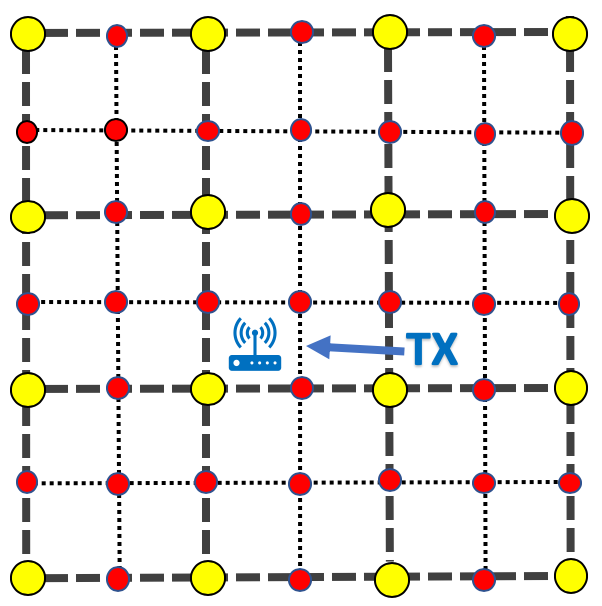
\includegraphics[width=0.45\textwidth]{chapters/ipsn/figures/multi-granular.png}
  \caption{Training for PDs at coarse-grained locations (yellow bigger
          dots), while estimating PDs using interpolation at the remaining
          fine-grained locations (red smaller dots).}
  \label{fig:path-loss}
\end{figure}

\para{Minimizing Training Cost with \ildw.} Consider a particular
location \lstar of a potential intruder. Our eventual goal is to
compute the PD for each of the $L$ possible sensor locations for this
location \lstar of a potential intruder; a PD may be computed either
by constructing it directly from gathered sensor observations or by
estimation via interpolation from the constructed PDs. In particular,
for effective interpolation, we construct PDs at coarser-grid sensor
locations and estimate via interpolation the PDs at the remaining
finer-grid locations. See Figure~\ref{fig:path-loss}. The exact
coarseness at which the PDs are constructed is determined by the
accuracy of the interpolation scheme for a given area and/or the
impact on localization accuracy due to estimated PDs. Below, we
describe the interpolation scheme that we use for our purposes.


\begin{figure}
  \begin{subfigure}[t]{0.9\textwidth}
    \centering
    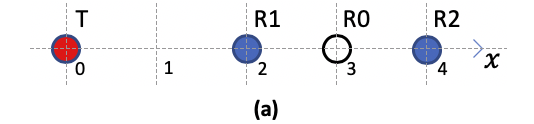
\includegraphics[width=0.5\textwidth]{chapters/ipsn/figures/interpolate.png}
  \end{subfigure}
  \qquad
  \newline
  \begin{subfigure}[t]{\textwidth}
    \centering
    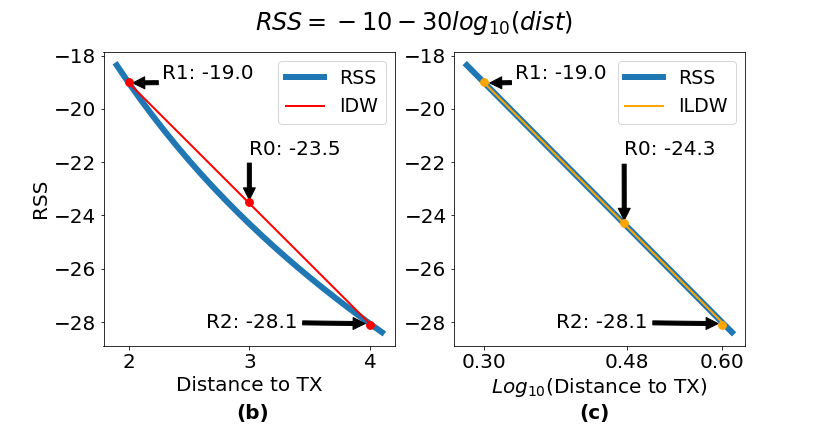
\includegraphics[width=0.8\textwidth]{chapters/ipsn/figures/ildw.png}
  \end{subfigure}
  \caption{Illustration of \ildw vs.\ IDW.
  (a) Transmitter (T), points with known (R1 and R2) and unknown (R0) received signal strength (RSS) values.
  (b) Log-normal RSS function (= -10 - 30$\log_{10}({\rm distance}))$
  plotted for varying distance from the transmitter $T$, along
  with IDW-estimated RSS value at a point between R1 and R2.
  (c) Log-normal RSS function and ILDW-estimated RSS value at
  a point between R1 and R2, plotted on a logarithmic distance
  scale.}
  \label{fig:ildw}
\end{figure}

\softpara{\ildw Interpolation Scheme.} Consider a fixed transmitter
location \lstar, and let us assume locations $\lo, \rt, \cdots, \lm$ for
which we know the path loss from \lstar. Now, consider a new point \lz
for which we wish to estimate the path-loss from \lstar.
%%%%%%%%%%%%
This is a traditional interpolation problem and well-known schemes
such as inverse distance weighting (IDW), Ordinary Kriging (OK), k-NN,
etc. have been evaluated even in the special context of signal
strength or received power~\cite{chakraborty2017specsense}.
%%%%
However, our specific context has a unique element. We
{\em know} the location \lstar of the transmitter from which the
path-loss is being estimated---as we are in the training phase wherein
we are gathering observations with the transmitter at \lstar.
\eat{ (ii) Second,
the points with known values viz.\ $\lo, \rt, \cdots, \lm$ are not
arbitrary or random points, but can be chosen to facilitate accurate
estimation (e.g., in our scheme, as mentioned above, we have chosen
them to be at coarser {\em uniform} grid locations).}
%%%%%%%%
In light of the above unique element of our setting, and the observation of wireless signal characteristics, we use a custom
interpolation technique which is a nontrivial modification of the IDW
scheme, called {\em inverse log-distance weighting} (\ildw). The traditional
IDW interpolation scheme estimates the
path loss at \lz by taking a weighted average of the path losses at
$\lo, \rt, \cdots, \lm$, with the weight being the inverse of the
distance from \lz. 
%%%%%

In our proposed \ildw scheme, we still estimate the path loss at \lz as
a weighted average of values at \li's, but assign weights differently.
In particular, we assign the weight for the point \li as the inverse
of the ``distance'' between \lz and \li in the domain where each point
is represented merely by its logarithmic distance from \lstar, the known
transmitter's location---i.e., each point $\li$ is mapped to a point
$\log d(\li, \lstar)$ on a line. This mapping is motivated by the
expectation that the actual path loss would be somewhat similar to the
log-distance path loss.
%%%%%%%
Thus, the weight for the point $\li$ is assigned to be
$$w_i = \frac{1}{|\log d(\li, \lstar) - \log d(\lz, \lstar)|},$$ where $d()$ is the
Euclidean distance function and the path loss at \lz is estimated as:
$$\uz = \frac{\sum_{i=1}^{n}w_i \ui}{\sum_{i=1}^{n}w_i},$$ where \ui
denotes the path loss at point \li from \lstar. In the above equation for
weights, if the denominator is zero, then we assign $w_i$ to be equal to
the maximum of the weights among the given points (and if all
denominators are 0, each weight is assigned to be 1).
%%%%%%%
For an illustration of the above scheme, see Figure~\ref{fig:ildw}.
In the IDW scheme, \lo and \lt will get equal weights, but under the
\ildw scheme they will get weights of $5.57$ and $8.00$
respectively. More importantly, it can be easily shown that, for
log-distance path loss, \ildw estimates the path loss for \lz accurately
from two unknown points \lo and \lt, if $d(\lo, \lstar) < d(\lz,
\lstar) < d(\lt, \lstar)$.

The above discussion has been on using \ildw for estimating path-loss
values. In general, it can be easily used to estimate PDs from the PDs
at neighboring points---essentially, we can use \ildw to estimate both
the mean and standard deviation of a Gaussian PD from other means and
standard deviations respectively.
%%\red{Note that it is important
%%  to insert a known value when TX and RX are at the same location.}

%% \softpara{Interpolation Scheme.}
%% . Many interpolation schemes  exisit OK, UK, IDW.
%% . Our problem is unique in the sense that the GIVEN points for which we know the f() values can be
%%   out own choice --- in particular, we have chosen them to be uniformly distributed.
%% . We choose IDW (inverse distance weighted) due to the uniformly distributed of given points and linearity of path-loss in log-normal model.
%% . Describe IDW briefly. 
%% . We are attracted by the simplicity and effectiveness of IDW.
%% . In fact, we modify IDW for our purposes to improve its performance. We call it ILDW. 
%% explore a new interpolation method by improving IDW with the knowledge
%% of wireless propagation characteristics, name it inverse log-distance
%% weighting (ILDW).

%% The basic idea of ILDW is to
%% give hutilize the fact that the RSS is theoretically linear to the logarithm
%% of distance.

%% \para{Interpolation Schemes.}
%% Many interpolation techniques have been explored for RF signals in
%% recent works~\cite heavily borrowing works from the geospatial
%% interpolation field.  Study~\cite{sigcomm15-workshop-interpolation}
%% shows Ordinary Kriging (OK), Universal Kriging (UK) and Inverse
%% Distance Weighting (IDW) are the top 3 methods with the least
%% interpolation error. ~\cite{montero2015spatial} notes that the
%% performance of UK deteriorates largely with decrease in density of the
%% observation data samples. So OK and IDW is our choice of pick.  Both
%% OK and IDW interpolate the value at a unknown point by giving some
%% weights to the known neighboring points and average them according to
%% the weights.  The difference is how to compute the weights.  Ordinary
%% Kriging is a widely used interpolation
%% method. ~\cite{chakraborty2017specsense} improves OK by applying the
%% knowledge of wireless propagation characteristics.
%% Signal strength
%% theoretically follows a log-normal pathloss model, where the received
%% signal strength can be given by
%% \begin{equation}
%% P - 10\alpha log_{10}(d) + N(0, \delta^2)
%% \label{equ:pathloss}
%% \end{equation}
%% where $P$ is the power at the transmitter, $d$ is the distance between
%% the transmitter and point of interest, and $N(0, \delta^2)$ reflects
%% fading and shadowing affects.  \ble{[describe why we don't use
%%     kringing.]}

\section{\texorpdfstring{\ouralgoss}: Localizing in Presence of Authorized Users}
\label{sec:auth}
\label{sec:mtlss}

We have implicitly assumed till now that the only transmitters present
in the area are the intruders which need to be localized.  In this
section, we adapt our \ouralgo approach described in the previous
section to the setting wherein there may be authorized transmitters in
the background and the localization technique must take their presence
into account. In particular, in a shared spectrum paradigm, there are
primary users and an evolving set of active secondary users
transmitting in the background. The key challenge comes from the fact
that the set of authorized users is not static and changes over time
as allocation requests are granted and/or active secondary users
become inactive over time.

One simple way to handle background users is to just localize every
transmitter, and then remove the authorized users. However, any
localization approach (including ours) is susceptible to performance
degradation with increase in number of transmitters to be localized,
especially if some of them are situated close together. Thus, this
simple approach of localizing every transmitter is unlikely to be
effective, as shown in our evaluations, especially when the number of
primaries and active secondaries can be large. Thus, here, we develop
an approach based on learning PDs in real-time in response to changes
in the set of secondary users.

\begin{figure}
	\centering
	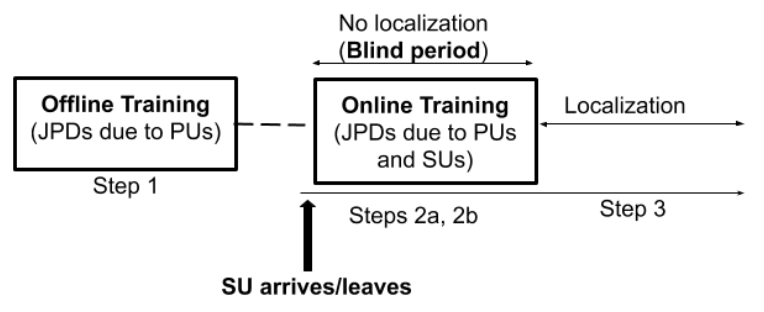
\includegraphics[width=0.7\textwidth]{chapters/ipsn/figures/map**2.png}
	\caption{\ouralgoss's overall approach}
	\label{fig:auth}
\end{figure}

\softpara{\ouralgoss: Localizing with Authorized Users}. Our problem
is to localize intruders in a shared spectrum system with fixed
primaries and changing set of secondaries.  Our \ouralgoss approach
uses a combination of a priori (offline) and online training to
construct JPDs for appropriate hypotheses based on gathered
observations, and then use these JPDs to localize intruders in
real-time using the \ouralgo approach described in the previous
section. We start with defining a few useful notations.

We use \Pa to denote the set of (fixed) primaries, and \Ka to denote
the set of secondaries at a given instant, and \ii to denote the \jth
configuration of intruders (we can assume the zero-th configuration to
represent no intruders). We use $\tau = \Pa \cup \Ka \cup \ii$ to denote the
set to all transmitters (authorized and unauthorized) at a given
instant.  Finally, we use $\pd(\vx | (\tau = X))$ to denote the joint
probability distribution (JPD) of observation vectors from the
deployed sensors when the prevailing hypothesis is that the set $\tau$
of transmitters is $X$. \ouralgoss is the sequence of following steps.
\begin{packedenumerate}
	\item
	(Offline Step.) Construct JPDs $\pd(\vx | \Pa)$ and $\pd(\vx | \tau = (\ii \cup \Pa))$ for all $j$. Since these JPDs 
	are independent of the secondaries, they do not change and
	can be done once a priori.
	\item
	(Online Steps.) Whenever \Ka (set of secondaries) changes:
	\begin{packedalpha}
		\item Construct JPD $\pd(\vx | \tau = (\Pa \cup \Ka))$. 
		\item Compute $\pd(\vx | \tau = (\Pa \cup \ii \cup
                  \Ka))$ for all $j$, from above constructed JPDs,
                  viz., $\pd(\vx | \Pa)$, $\pd(\vx | \tau = (\ii \cup
                  \Pa))$, and $\pd(\vx | \tau = (\Pa \cup \Ka))$. See
                  the below observation.
	\end{packedalpha}
	\item
	(Real-time Localization.) Periodically, each sensor sends its
          observation to a centralized entity (spectrum
          manager) which uses \ouralgo to localize any intruders
          present. Here, localization essentially means determining
          the most likely prevailing hypothesis among the hypotheses
          $\tau = (\Pa \cup \ii \cup \Ka)$, based on the JPDs $\pd(\vx | \tau = (\Pa \cup \ii \cup \Ka))$ constructed in earlier
          steps.
\end{packedenumerate}

Note that steps 1 and 2a are essentially learning the authorized users' signal charecteristics and view them as the "background signals". 
If there are no authorized users, then the background signals are "quite". Else, then the background signals have some "sound".
We now state the observation that forms the basis of JPD computation
in Steps 2b; note that the noise due to sensor's hardware gets
duplicated when ``adding'' two JPDs, but can be easily removed.
\begin{obs}
  The JPD $\pd(\vx | (\tau = A \cup B))$ and be computed from JPDs $\pd(\vx | (\tau = A))$ and $\pd(\vx | (\tau = B))$.  Similarly,
  JPD $\pd(\vx | (\tau = A))$ can be computed from the JPDs $\pd(\vx | (\tau = A
\cup B))$ and $\pd(\vx | (\tau = B))$.
\end{obs}

\para{Blind Period due to Step 2.}  Note that the steps 2a and 2b
construct or compute the JPDs needed for localization, and thus,
during their execution, the localization cannot be done. Thus, it is
important that the duration of this ``blind period'' in
minimal. Fortunately, step 2b being a simple mathematic computation
takes only in the order of milliseconds under efficient implementation, while 2a merely entails gathering a
sufficient number of observations to construct the desired JPD which
could take anywhere from milliseconds to a few seconds, as an
observation takes only a fraction of a millisecond~\cite{our-infocom}.

\para{Mobility of Users and Sensors.}  We note that \ouralgo works
seamlessly for mobile intruders and sensors, due to the constructed
PDs. However, \ouralgoss has the following limitation: the sensors
must remain static in between two consecutive online-training periods
(i.e., step 2 of above). If a sensor $X$ moves, then either $X$'s
observation must be ignored, or that $X$ needs to online-train itself
in its new location (and there should be no intruders during this
individual online-training phase). Note that active SUs are expected
to remain static anyway, as they are allocated spectrum for a specific
location.

%% . Mobility: PUs are static. (else the offline and online training needs to be redone).
%%             Active SUs static (otherwise online learning needs to be redone, if they move).
%%             Intruders can move --- each time window localizes intruders at that instant of time.
%%             Sensors. Cannot move during the period between change of active SUs. If they do, then retraining
%%                      needs to be done. 

\section{Large-Scale Simulation Results}
\label{sec:eval}

To evaluate our techniques in a large scale area (a few kms square),
we conducted simulations over a geographic area using path-loss values
from the Longley-Rice propagation model generated by
open sourse software SPLAT!~\cite{splat}. We describe the simulation setting below and
discuss the results.

\subsection{Settings}

\para{Generating Probability Distributions.} To evaluate our
techniques over a large area with 100s of sensor nodes, we need to run
simulations with an assumed propagation model. We use the well-known
Longley-Rice ~\cite{lr} Irregular Terrain With Obstruction Model (ITWOM), 
which is a complex model of wireless
propagation based on many parameters including locations, terrain
data, obstructions and soil condition etc. and such.
%%%%%%%%%%%%
We consider an area of 4km $\times$ 4km in the NY state and use the
800 MHz band for SPLAT! We discretize the area using 40 vertical and
40 horizontal grid lines---yielding 1600 cells each of size 100m
$\times$ 100m.
%\red{Each cell represents a discrete location.}
%%%%%%
To generate a probability distribution (PD) at a sensor location $x$
due to a transmitter at location $l$ transmitting at power $\pstar$,
we compute the received power at $x$ using transmit power minus path-loss from SPLAT!, and use it as the mean of the probability distribution. For the
complete PD, we assume Gaussian distributions and use a standard
deviation between 1 and 3, with higher values for pairs $(x,l)$ with
smaller distance.
%%%%%%
As mentioned before, the PD due to multiple simultaneous transmitters
can be computed as just a ``sum'' of the Gaussian distributions due to
individual transmitters~\cite{rappaport-2001,mobicom17-splot}.
%% \ble{The expectation of power of the sum of multiple signals is equal
%%  to the sum of power of the individual signals
%%  ~\cite{rappaport-2001}.  ~\cite{mobicom17-splot} validates this by
%%  conducting experiments in the Orbit testbed.}

\para{Algorithms Compared.}  For the \mtl problem, we compare our
\ouralgo algorithm with \splot~\cite{mobicom17-splot} and
\cl~\cite{clustering} (see \S\ref{sec:ipsn-related}). As mentioned
before,~\cite{Quasi-EM} has been shown to be inferior in performance
to both \splot and \cl in their respective works, and thus, not
evaluated here.
%%%%%%
\cl uses $k$-means~\cite{scikit-learn} for clustering, and needs to be
provided with the number of clusters. To do a somewhat fair
comparison, we provide \cl with a {\em range} of the number of
intruders and use the elbow-point method to pick the best
number of clusters/intruders. In particular, the range of intruders
passed to \cl is 1 to $2x$, where $x$ is the actual number of
intruders present.
%%%%%%%%%
\begin{table}[ht]
	\caption{Simulation Evaluation Parameters.}
	\centering
	\begin{tabular}{c c c c}
		\hline\hline
		Param. & Value & Description \\ [0.5ex]
		\hline
		$Q^{'}_{1}$ &  0.6   & Threshold for Procedure 1's hypothesis posterior\\ 
		$Q^{'}_{2}$ &  0.1   & Threshold for Procedure 2's hypothesis posterior\\
		$R$  & 1000 & Transmission radius when power is \pstar, (m) \\
		\pstar & 30  & Transmit power during training, (dBm) \\
		$\delta_p$ & 2  & Range of intruders' power is $[\pstar - \delta_p, \ \pstar + \delta_p]$\\
		\hline
	\end{tabular}
	\label{table:paramaters}
\end{table}

For \splot, we use the same set of parameters values as
in~\cite{mobicom17-splot} except that we use the confined area radius
to be 800m for our large area setting (\cite{mobicom17-splot} only
considered small 15m $\times$ 15m areas; 800m is roughly the maximum
transmission radius in our large-scale setting and other values
yielded worse results).
%%%%%%
Table \ref{table:paramaters} gives the main parameters of \ouralgo
used in our evaluations. Recall that the transmission radius is the
distance between the TX and RX for which the RX's RSS is at the noise
floor (we use -80dBm). \eat{Issues: Threshold for SPLOT, further explain $STD_1$ and
  $STD_2$}

\begin{figure}[ht]
	\centering
	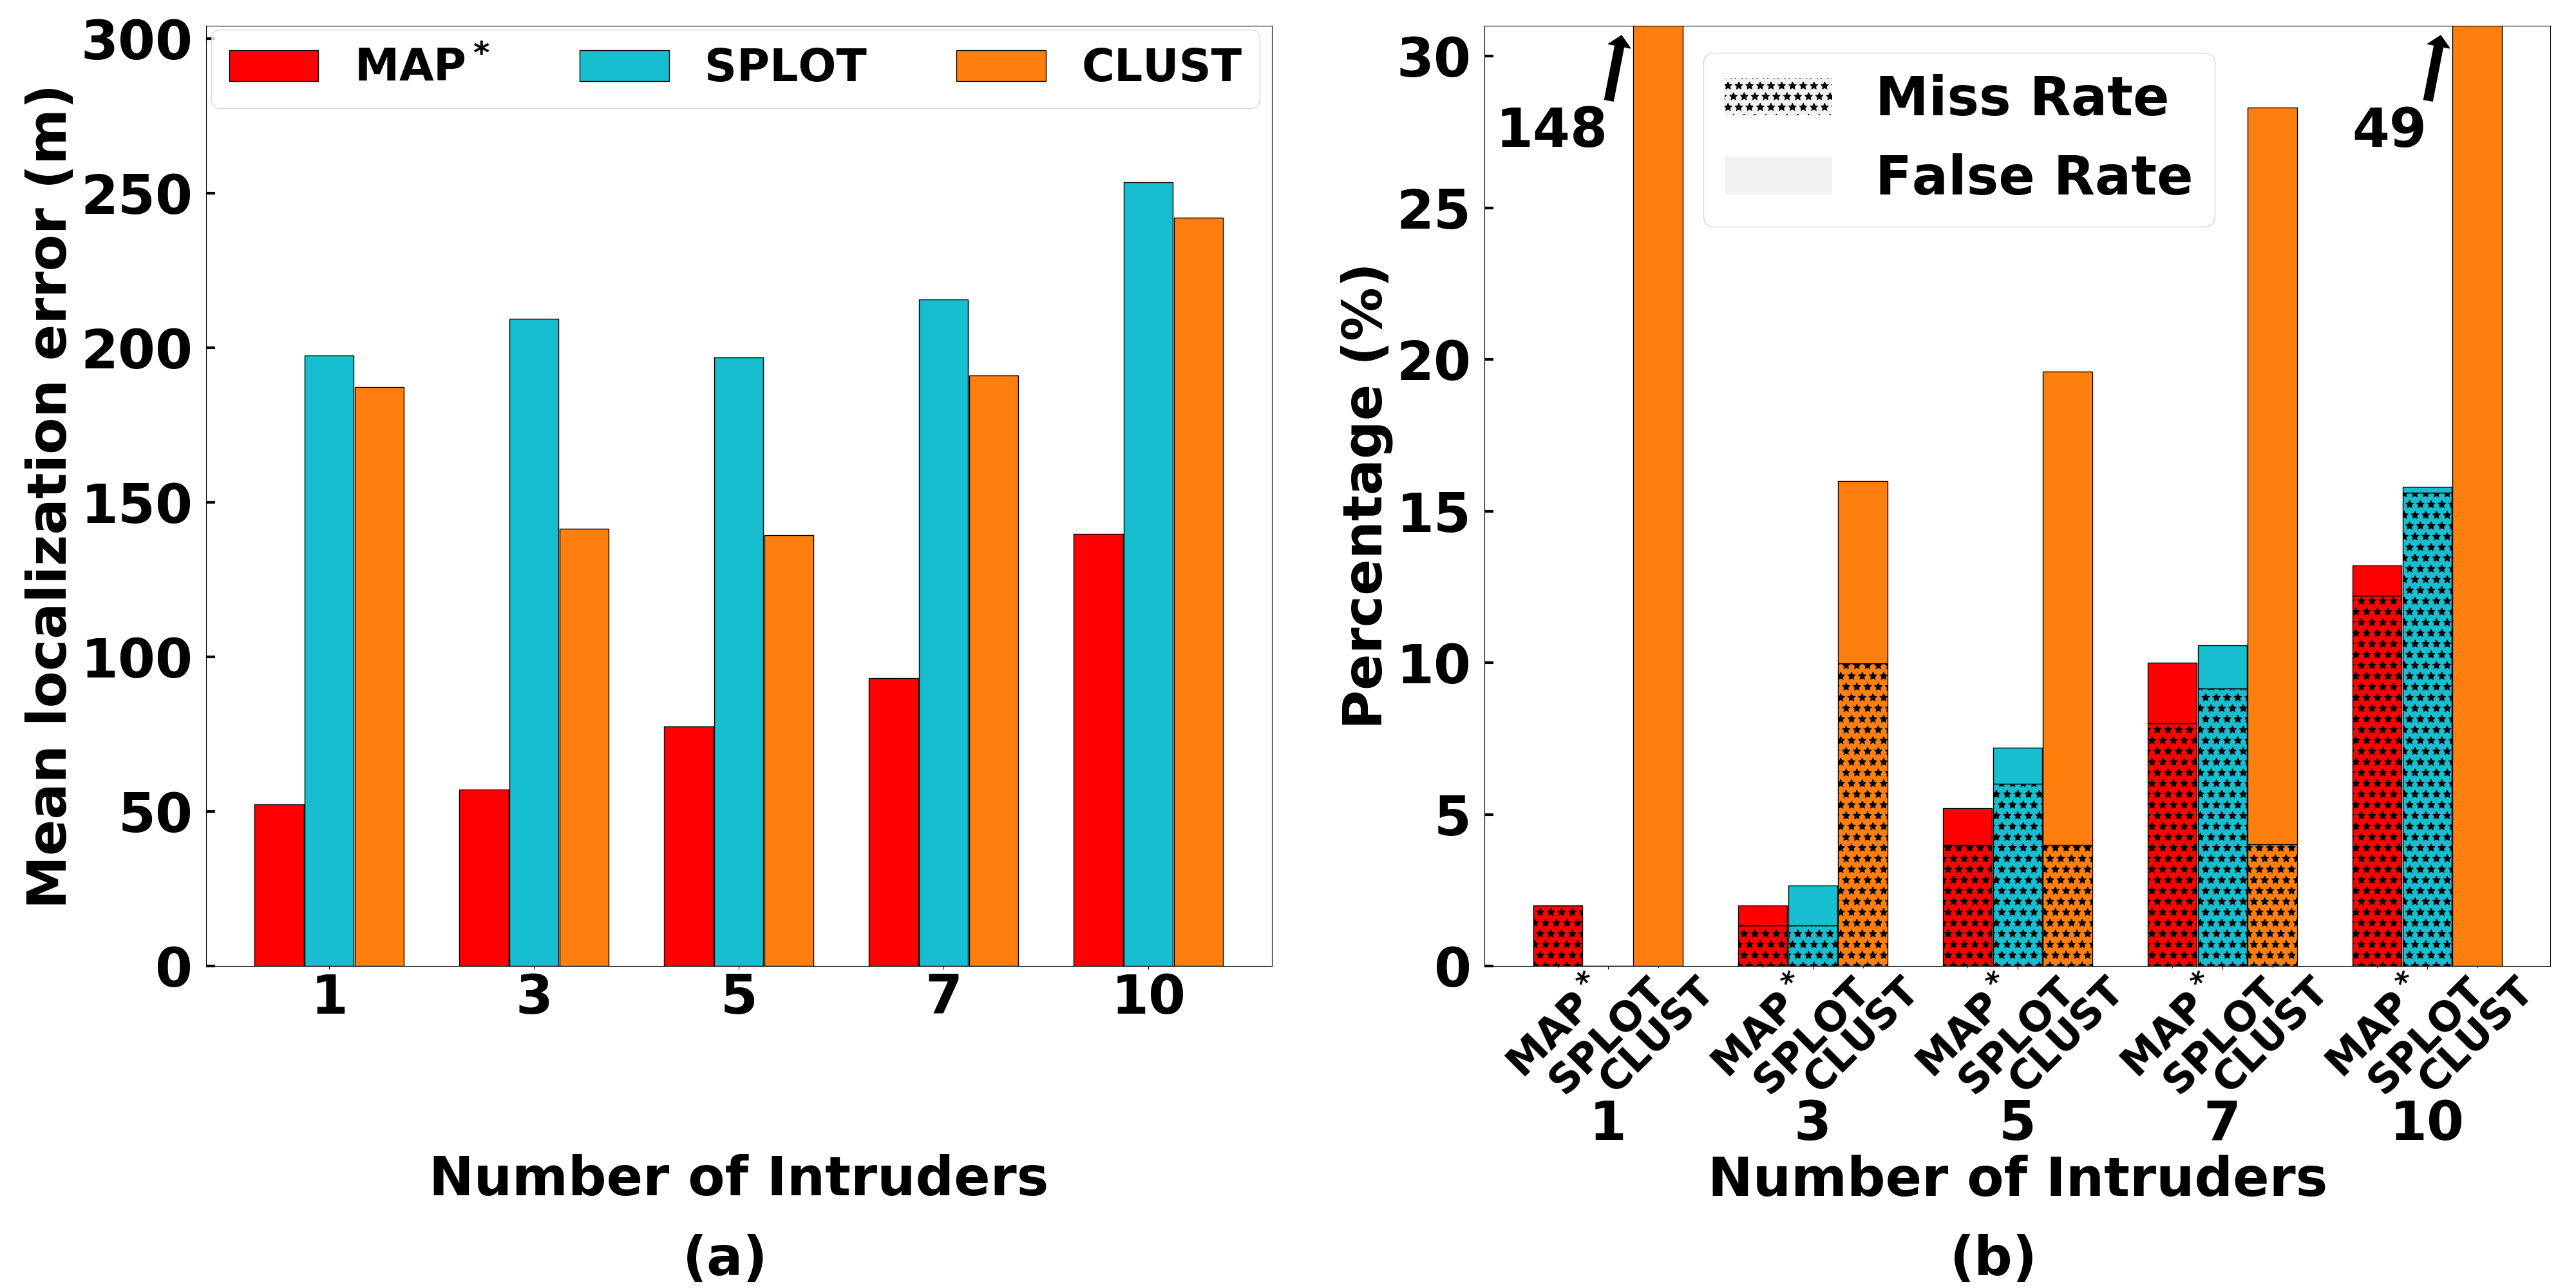
\includegraphics[width=0.8\textwidth]{chapters/ipsn/figures/splat-vary-numintru.png}
	\caption{Localization performance of various algorithms in a large scale area, for varying number of intruders}
	\label{fig:varying-num-intruders}
\end{figure}

\subsection{Five Evaluation Metrics.}
We use the following metrics to evaluate the localization methods. 
\begin{enumerate}
\item Localization error ($\lerr$). 
\item Miss rate ($\mr$).
\item False alarm rate ($\fr$).
\item Power error ($\perr$).
\end{enumerate}
The above metrics are best explained using a simple example. Given a
multi-intruder localization solution, we first compute the $\lerr$ as
the minimum-cost matching in the bi-partite graph over the
ground-truth and the solution's locations, where the cost of each edge
in the graph is the Euclidean distance. We use a simple greedy
algorithm to compute the min-cost matching.
%%%%
The unmatched nodes are regarded as false alarms or misses. E.g., if
there are 4 intruders in reality, but the algorithm predits 6
intruders then it is said to incur 0 misses and 2 false alarms and if
it predicts 3 intruders then it incurs 1 miss and 0 false alarms. The
$\mr$ and $\fr$ metrics are on a per-intruder basis, so in the above
two examples: $\mr$ is 0 and 1/4 and $\fr$ is 2/4 and 0. In the plots, we stack miss rate and false alarm rate together to show the overall difference between the true number of intruders and predicted number of intruders.
%%%%%%%
$\perr$ is the average difference between the predicted power
and the actual power of the matched pair in the above bi-partite
graph. 

Finally for interpolation schemes, we use the metric (5) interpolation error ($\ierr$) defined as the estimated path-loss minus the ground-truth path-loss value.

\subsection{Results}

In this subsection, we evaluate the performance of our techniques for
varying parameter values, viz., number of intruders and sensors in the
field, and training cost.
%%%%%%%%
Here, the training cost is defined relative (specifically, as a
percentage of) to the full training scenario wherein we construct each
of the $1600 \times 1600$ PDs (one for each pair of transmitter and
sensor locations) directly from observations. E.g., $x\%$ training
cost indicates that we construct $1600 \times (16x)$ PDs directly, and
interpolate the remaining $1600 \times (1600-16x)$ PDs; our proposed
interpolation scheme only interpolates for sensor locations.
%%%%%%
In general, when we vary a specific parameter, the other parameters
are set to their default values which are: 9\% for training
cost, 5 for number of intruders, and 240 for number of sensors.
%%%%%
For each experiment, the said number of sensors and intruders are
deployed randomly in the field, with the intruders deployed in the
continuous location domain while the sensors deployed only at the
centers of the grid cells. Each data point in the plots is an
average of 50 experiments.

\begin{figure}[ht]
	\centering
	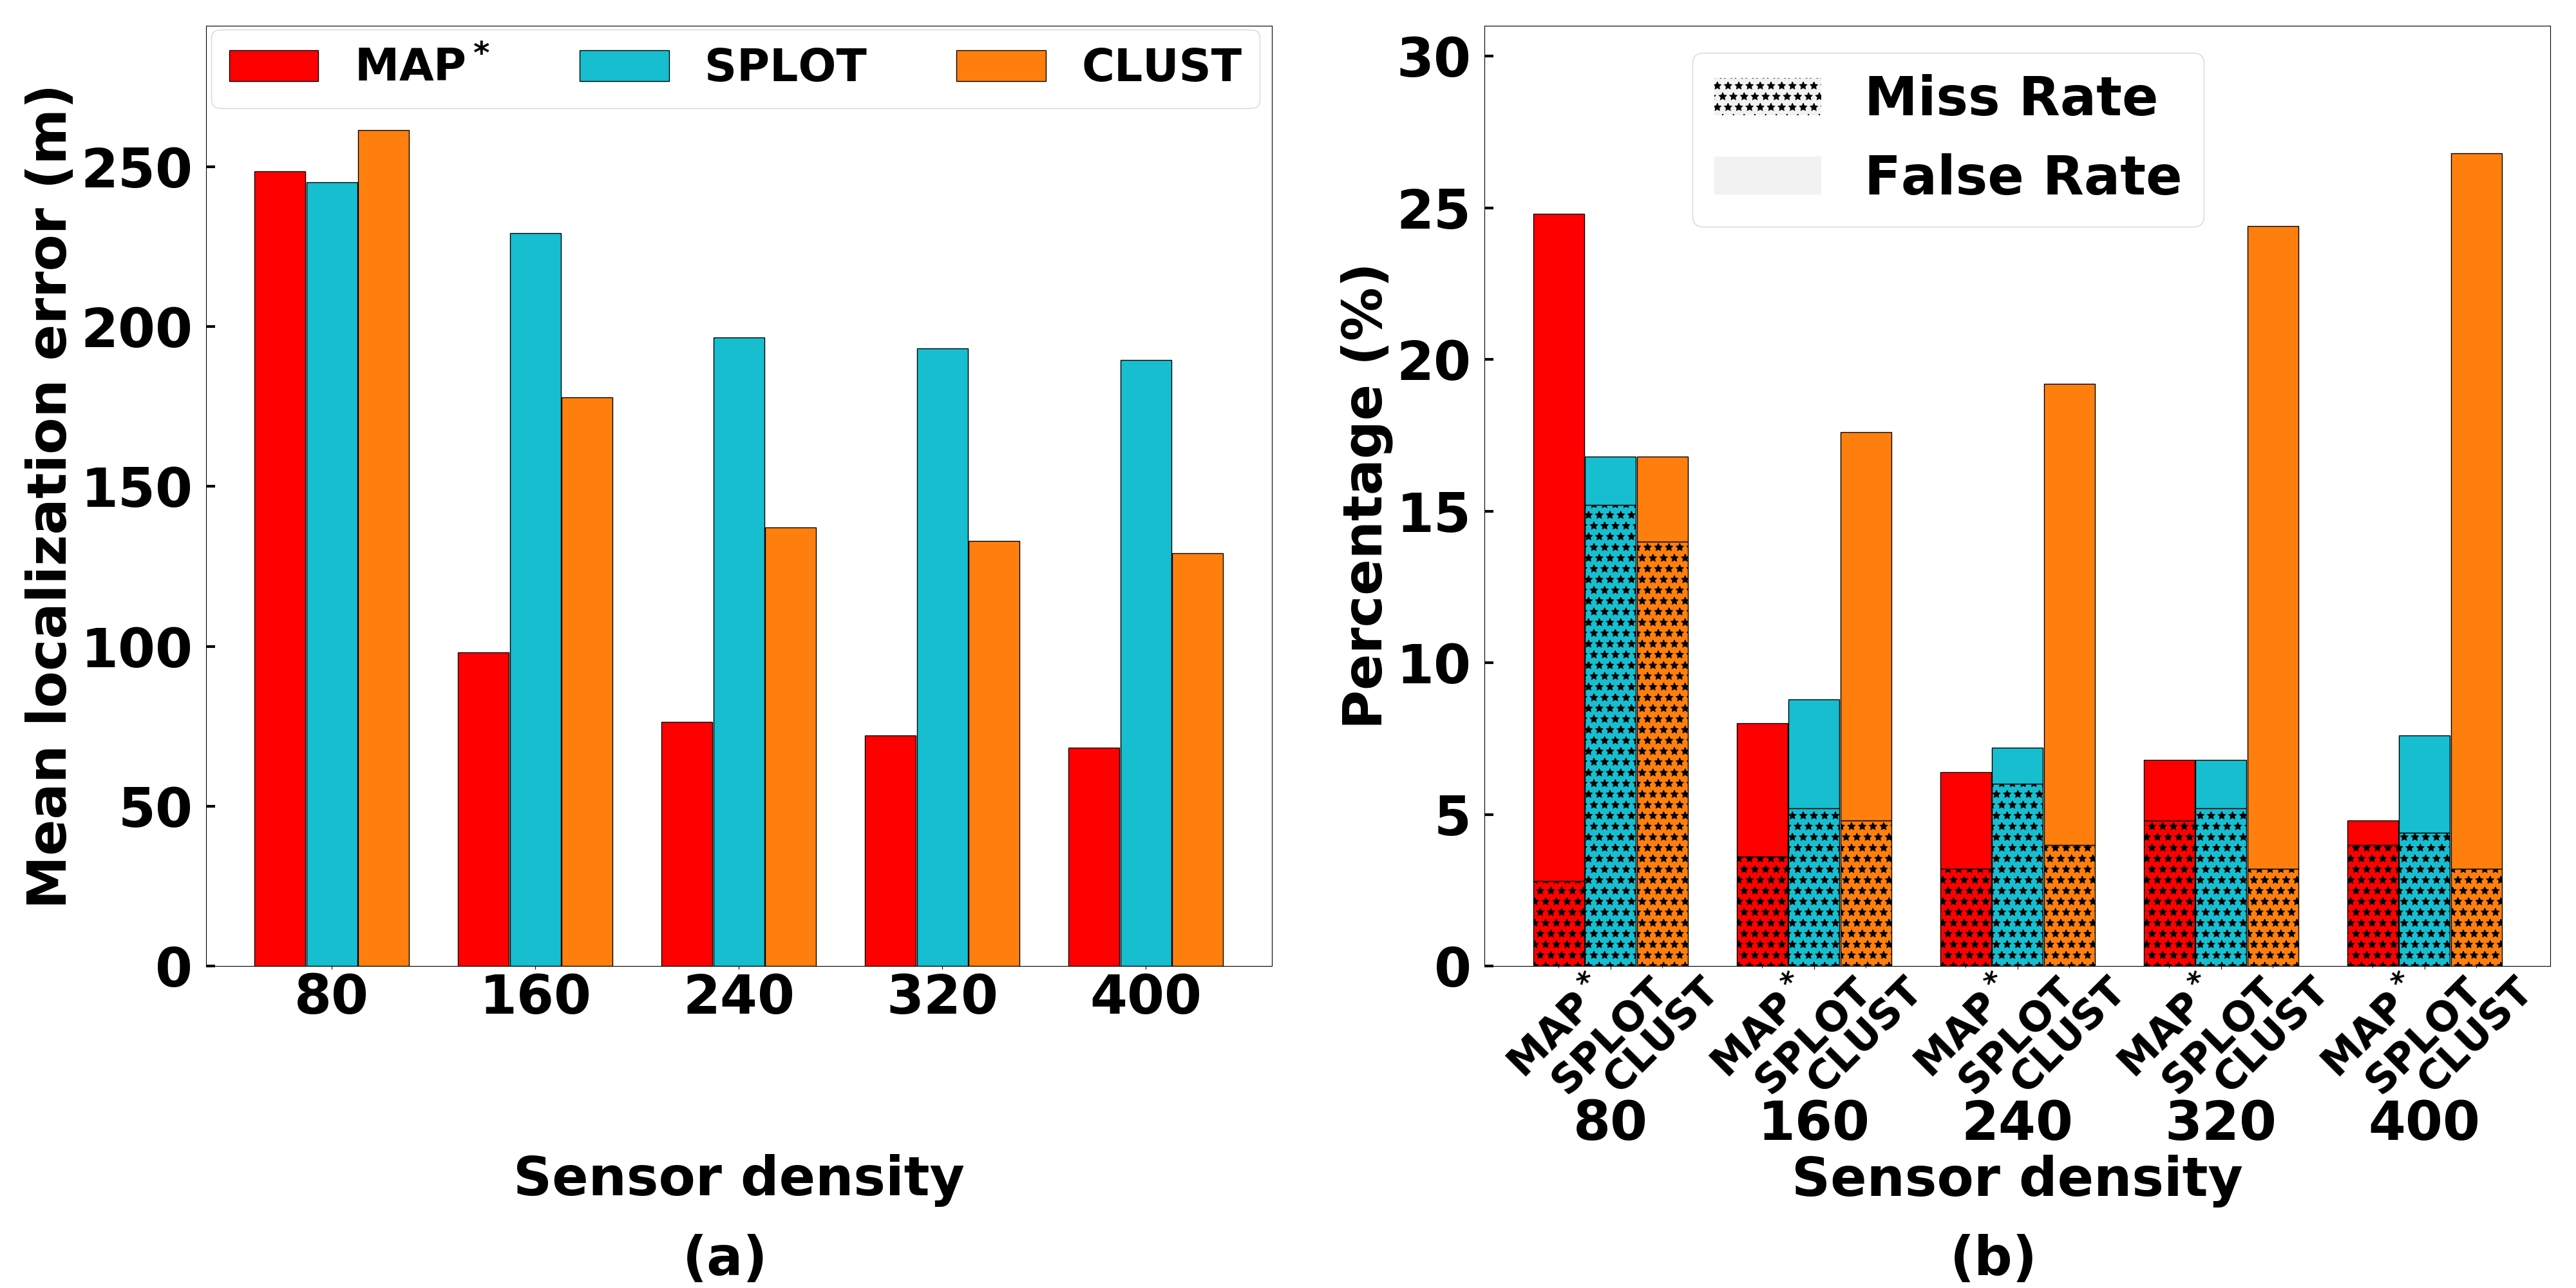
\includegraphics[width=0.8\textwidth]{chapters/ipsn/figures/splat-vary-sendensity.png}
	\caption{Localization performance of various algorithms in a large scale area, for varying sensor density}
	\label{fig:varying-num-sendensity}
\end{figure}

\para{Varying Number of Intruders.}  First, we compare the
localization accuracy of various algorithms for varying number of
intruders.  See Figure \ref{fig:varying-num-intruders}. We vary the
number of intruders from 1 to 10. We observe that the localization
error of \ouralgo is the minimum across the three algorithm. 
The localization error is 45\% -- 74\% less than \splot.
In terms of the $\mr$ and $\fr$, \ouralgo also performs others which confirms the overall performance
of \ouralgo to be the best among the algorithms compared. In terms of
absolute performance, note that the localization error of 50-150m
indicates an error of 1-2 grid cells, and thus is minimal in the
context of the large area of 4km by 4km with 1600 cells and a sensor
population of 240. Investigating further, we observe that misses in
\ouralgo are mostly due to the interpolated PDs (note that only 9\% of
the PDs are constructed from the actual sensor observations, and the
remaining 91\% are interpolated), while \splot's misses are mainly
from the case of two or more intruders being close to each other. This
demonstrates the superior ability of \ouralgo to localize intruders
that are close-by via the designed sequence of Procedures 1 and 2.


\begin{table}
	\caption{\ouralgo Power Error (dB) }
	\centering
	\begin{tabular}{c c c} 
		\hline\hline
		\# Intru. & MAE & ME \\ [0.5ex]
		\hline
		1 & 0.56  & -0.07  \\ 
		3 & 1.02  & 0.89 \\
		5 & 1.31  & 0.97 \\
		7 & 1.52  & 1.16 \\
		10 & 1.47 & 1.04 \\
		\hline
	\end{tabular}
	\label{table:splat-power-error}
\end{table}

\begin{table}
	\caption{Running time (s)}
	\centering
	\begin{tabular}{c c c c}
		\hline\hline
		\# Intru. & \ouralgo & \splot & \cl \\
		\hline
		1 &  0.55 & 0.56 & 0.03\\ 
		3 &  1.07 & 1.02 & 0.11  \\
		5 &  5.74 & 1.35 & 0.23 \\
		7 &  8.14 & 1.63 & 0.30 \\
		10 & 16.50 & 1.89 & 0.41  \\
		\hline
	\end{tabular}
	\label{table:splat-running-time}	
\end{table}


\softpara{Intruder Power Estimation, and Computation Time.}
Table~\ref{table:splat-power-error} shows the mean absolute error
(MAE) and mean error (ME) of the intruder's predicted power by
\ouralgo. Note that \cl and \splot do not predict intruder's power,
and hence, not shown. We observe that \ouralgo is able to predict
intuder's power quite accurately. The errors increase with the increase in number of intruders. Also, the mean error begins at near zero and then turns positive. 
%%%%%
Table~\ref{table:splat-running-time} shows the running time of various
algorithms over an Intel i7-8700 3.2 GHz processor. We see that \cl is
the fastest, and the running times of \ouralgo and \splot are
comparable for small number of intruders, but for larger number of
intruders, \ouralgo takes longer time than \splot mainly because of
more number of iterations of the computationally-intensive Procedure
2.

\begin{figure}[ht]
	\centering
	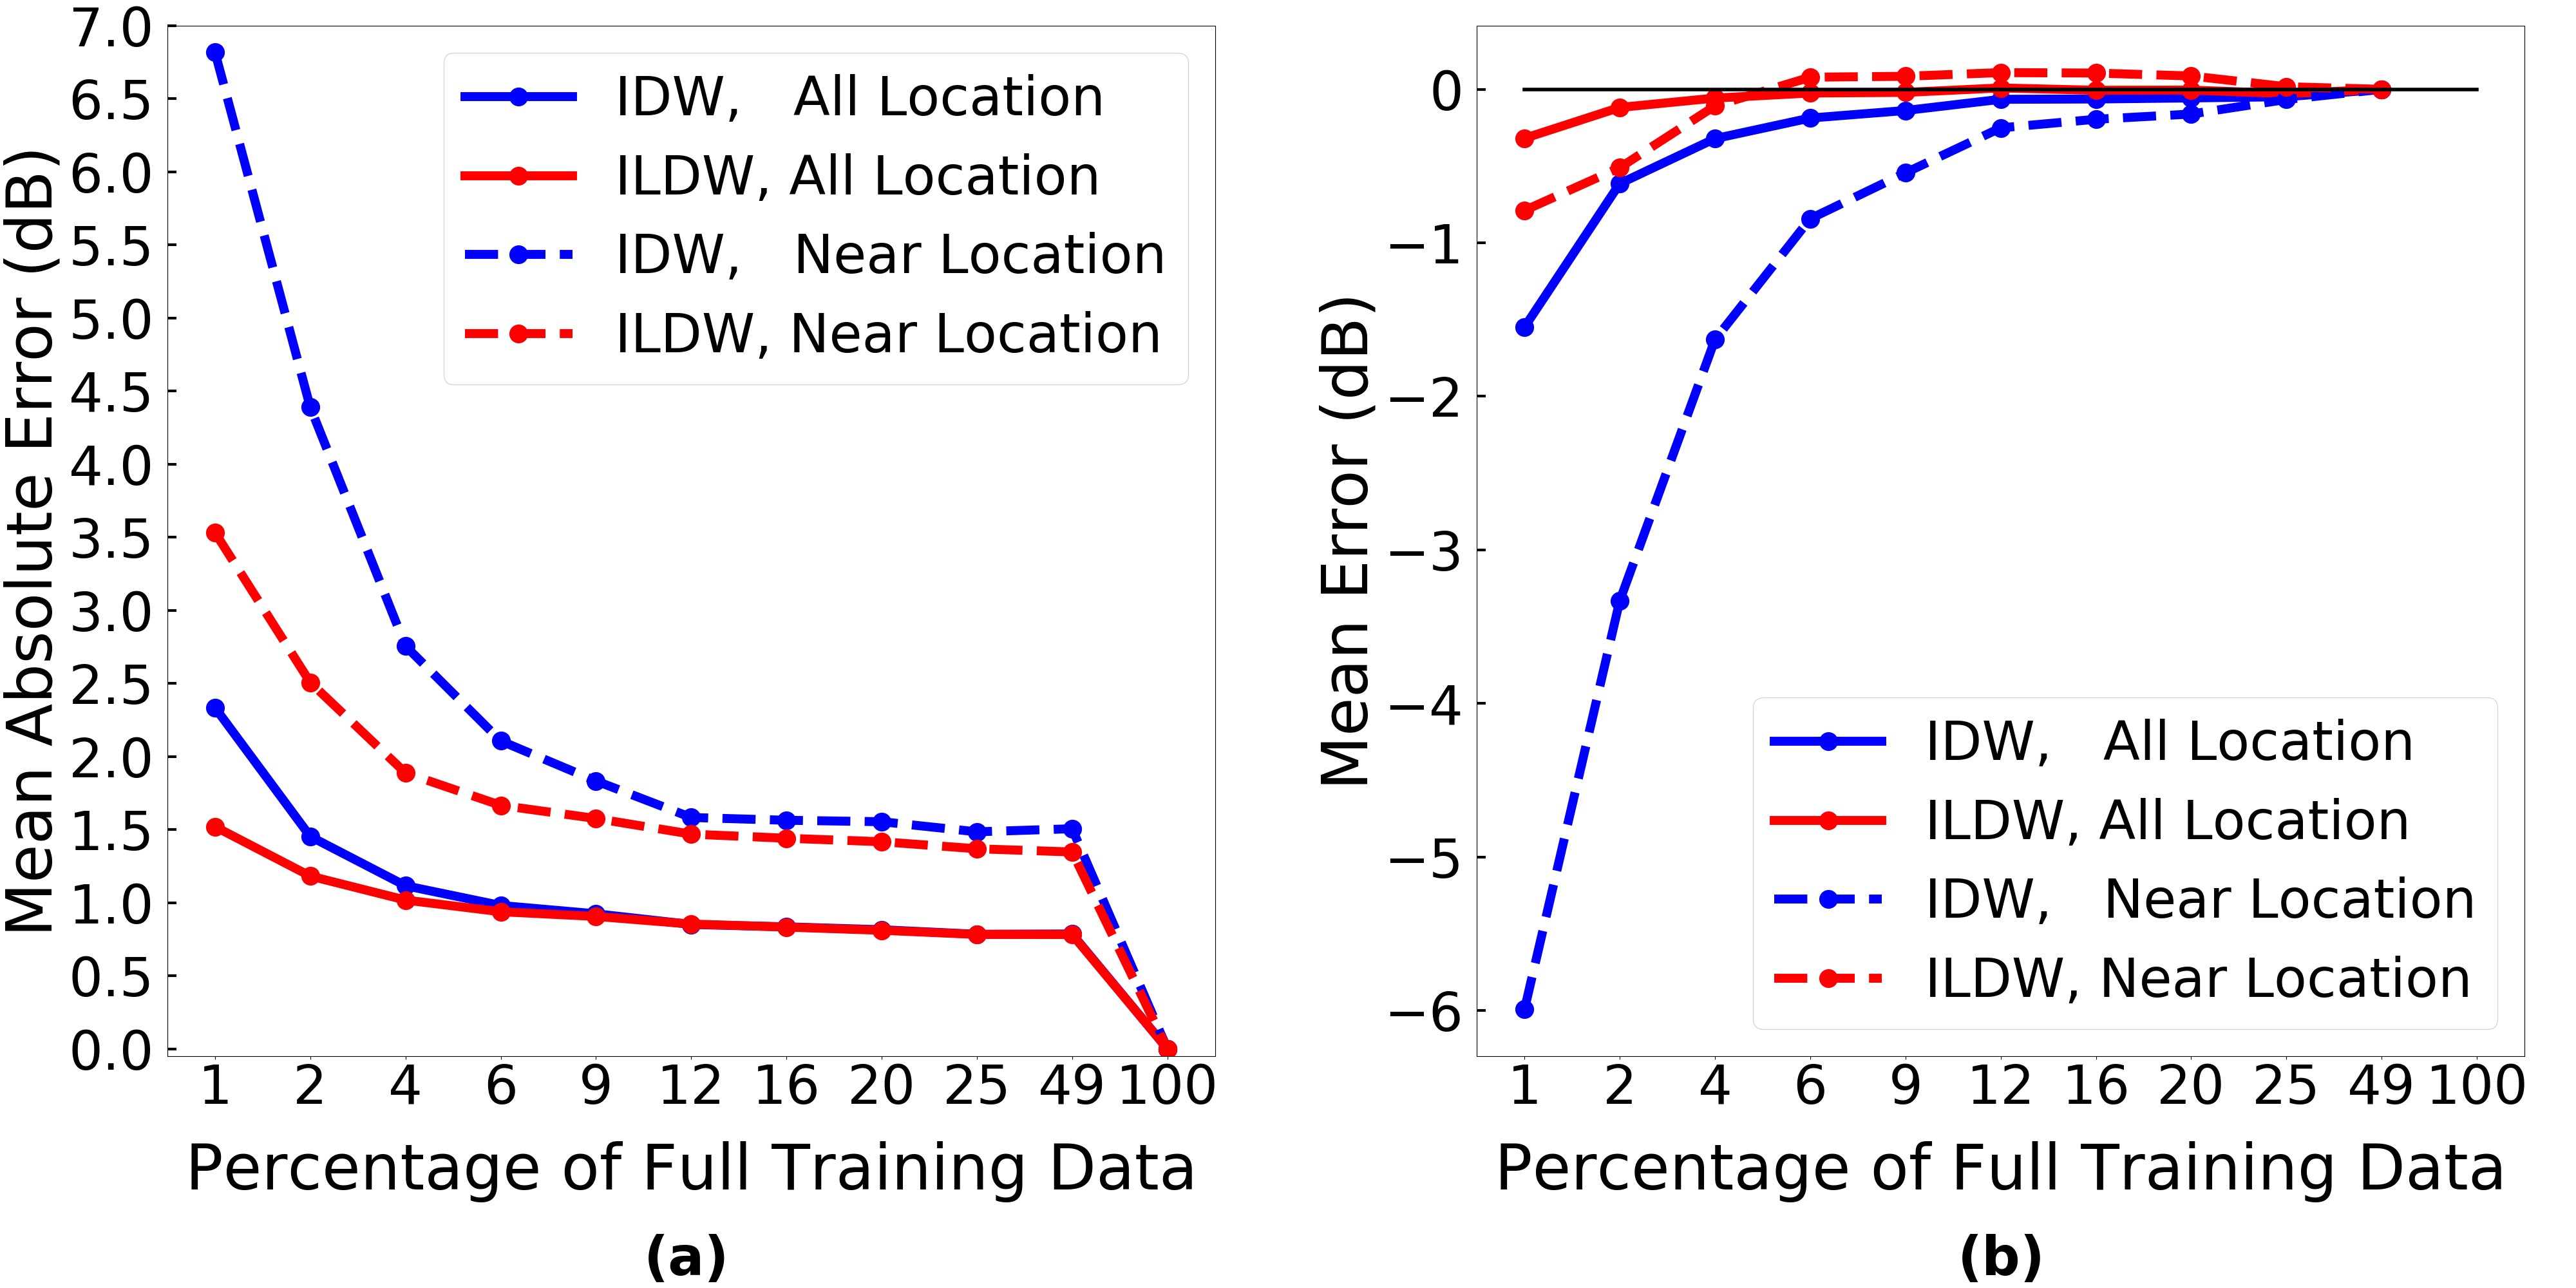
\includegraphics[width=0.8\textwidth]{chapters/ipsn/figures/inter_error.png}
	\caption{Estimation errors for interpolation schemes for varying training data}
	\label{fig:inter-error}
\end{figure}

\para{Varying Sensor Density.} We now vary the total number of sensors
in the field, and observe the impact on the performance of various
algorithms. See Figure \ref{fig:varying-num-sendensity}, where the
number of sensors is varied from 80 to 400. We see that all algorithms
perform better with increasing number of sensors as expected, with
\ouralgo performance improving significantly (in both $\lerr$ as well
as $f_r + m_r$) as number of sensors is increased from 80 to 160. More
importantly, except for very low number of sensors (i.e., 80),
\ouralgo handily outperforms the other two algorithms.


\para{Varying Training Cost.}  Finally, we now investigate how the
training cost (i.e., number of PDs constructed from raw observations)
affects the performance of our \ouralgo algorithm. Note that the other
algorithms do not depend on the training data, hence not shown.
%%%%%%%%%%
We first evaluate the interpolation error of our \ildw scheme for
varying training cost (number of known PDs) by comparing with the
traditional IDW scheme on which it is based. See
Figure~\ref{fig:inter-error}, which plots the mean absolute error
(MAE) as well as mean error (ME). As the interpolation error is
substantially higher for points that are closer to the transmitter, we
plot MAE and ME as averaged over all interpolated points as well as
over just the points close (less than 800m away) to the transmitter. Note
that the PDs at sensor locations closer to the transmitter would have
a stronger bearing on the localization accuracy, and thus, the MAE and
ME values for points closer to the transmitter are of more
significance.
%%%%%
We observe here that as expected both MAE and (absolute value of) ME
decrease with increase in the training cost for both \idw and \ildw,
but MAE and ME of \ildw is significantly lower than that of \idw
especially for low percentages of training cost and when the points
are close to the transmitter.
%\rd{HG: I want to remove the following
 % sentence.}  \ble{This shows that weighting the neighbors in the
  %logarithm scale towards the transmitter mitigates the negative
  %trend.}

We now plot the performance of \ouralgo for varying training data; see
Figure~\ref{fig:varying-training-data}. As expected, the performance
metrics show general improvement with increase in amount of
training. More importantly, we note that with 5-10\% of training,
\ouralgo achieves performance comparable to that with 100\% training,
suggesting that our interpolation scheme is largely effective as long
as 5-10\% of PDs are constructed from raw observations. 
\eat{TODO \red{Put Fig 7+8,
  9+10 in the same ROWs as Fig 7(a)-(b) and 8(a)-(b). will look better.}}



\begin{figure}[ht]
	\centering
	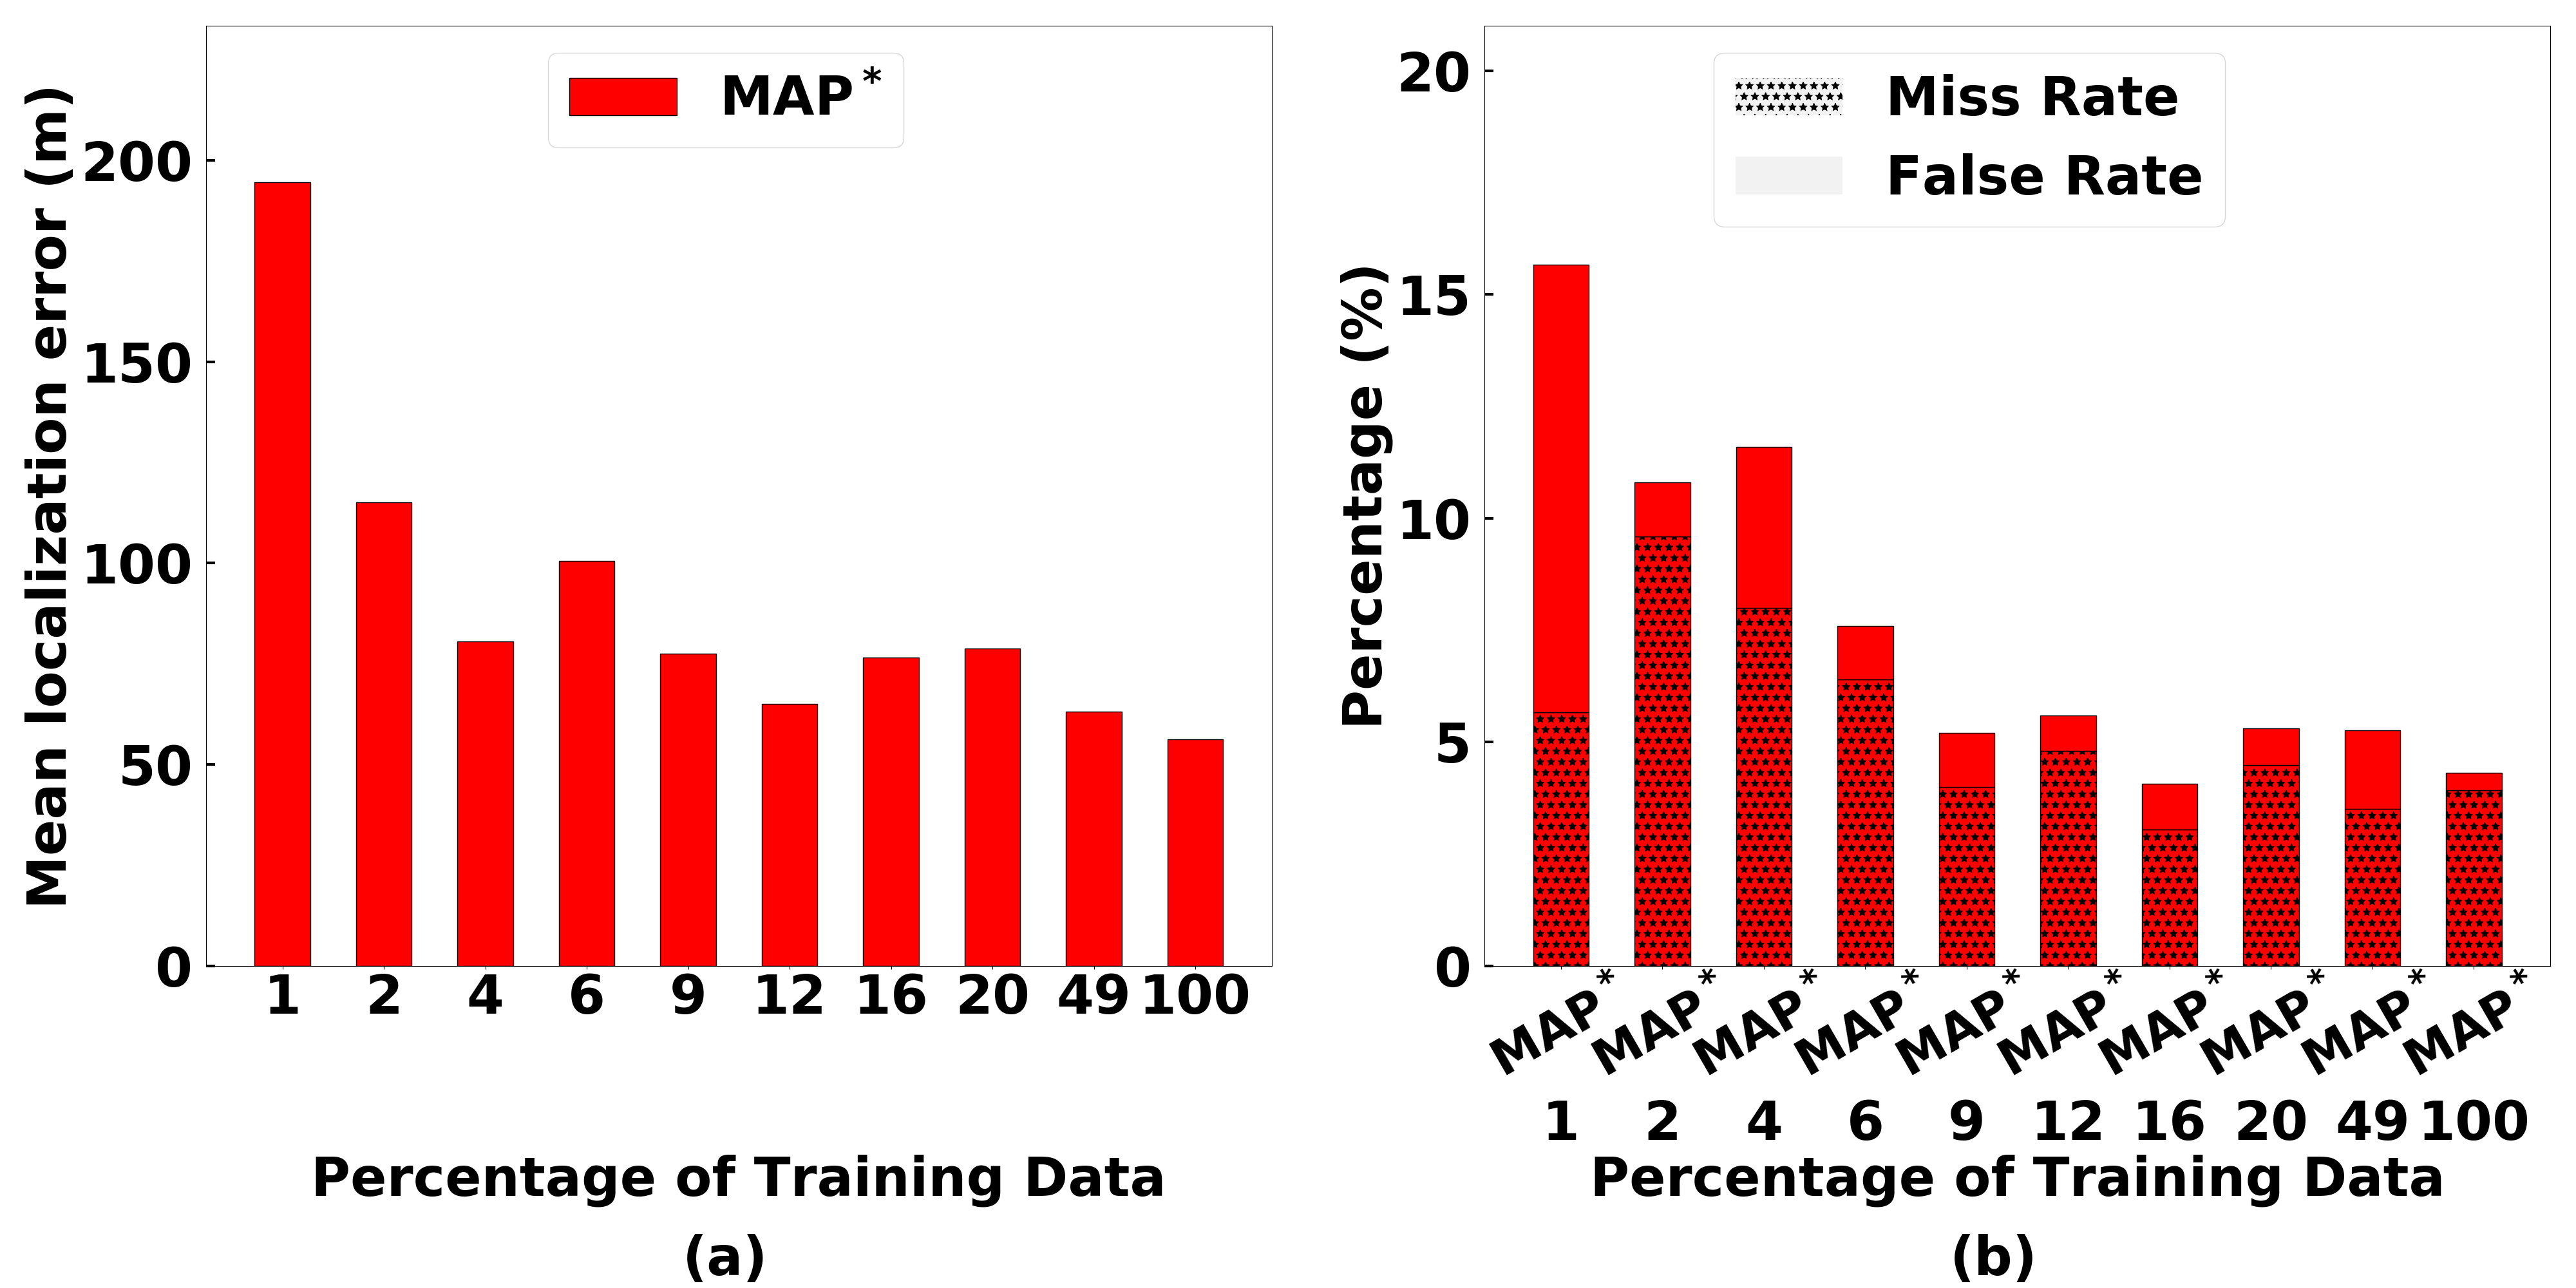
\includegraphics[width=0.8\textwidth]{chapters/ipsn/figures/splat-vary-training.png}
	\caption{Localization performance of \ouralgo in a large scale area, for varying training data}
	\label{fig:varying-training-data}
\end{figure}

\para{In Presence of Authorized Users (\ouralgoss).}  We now evaluate
the performance of our \ouralgoss approach which is tailored to work
in the presence of authorized users. To evaluate \ouralgoss, we place
5 authorized users in the area---with 2 primary and 3 secondary users.
The primary users are placed at fixed locations, while the secondaries
are put at random locations. We assign each authorized user a random
power in the range of 30 to 32dBm, while, as before, a random power
between 28 and 32dBm to the intruders. To ensure that these 5
authorized users do not ``interfere'' with each other, we ensure that
the distance between any two of these authorized users is at least
1000m.
%%%%%%%%%
We compare \ouralgoss with the simpler approach called \ouralgos that
uses \ouralgo to localize all transmitters (authorized as well as
intruders) and then removes the predicted transmitters that are
closest to the authorized users.
%%%
See Figure \ref{fig:shared-spectrum}, which shows that \ouralgoss easily
outperforms \ouralgos for varying number of intruders. 

\begin{figure}[ht]
	\centering
	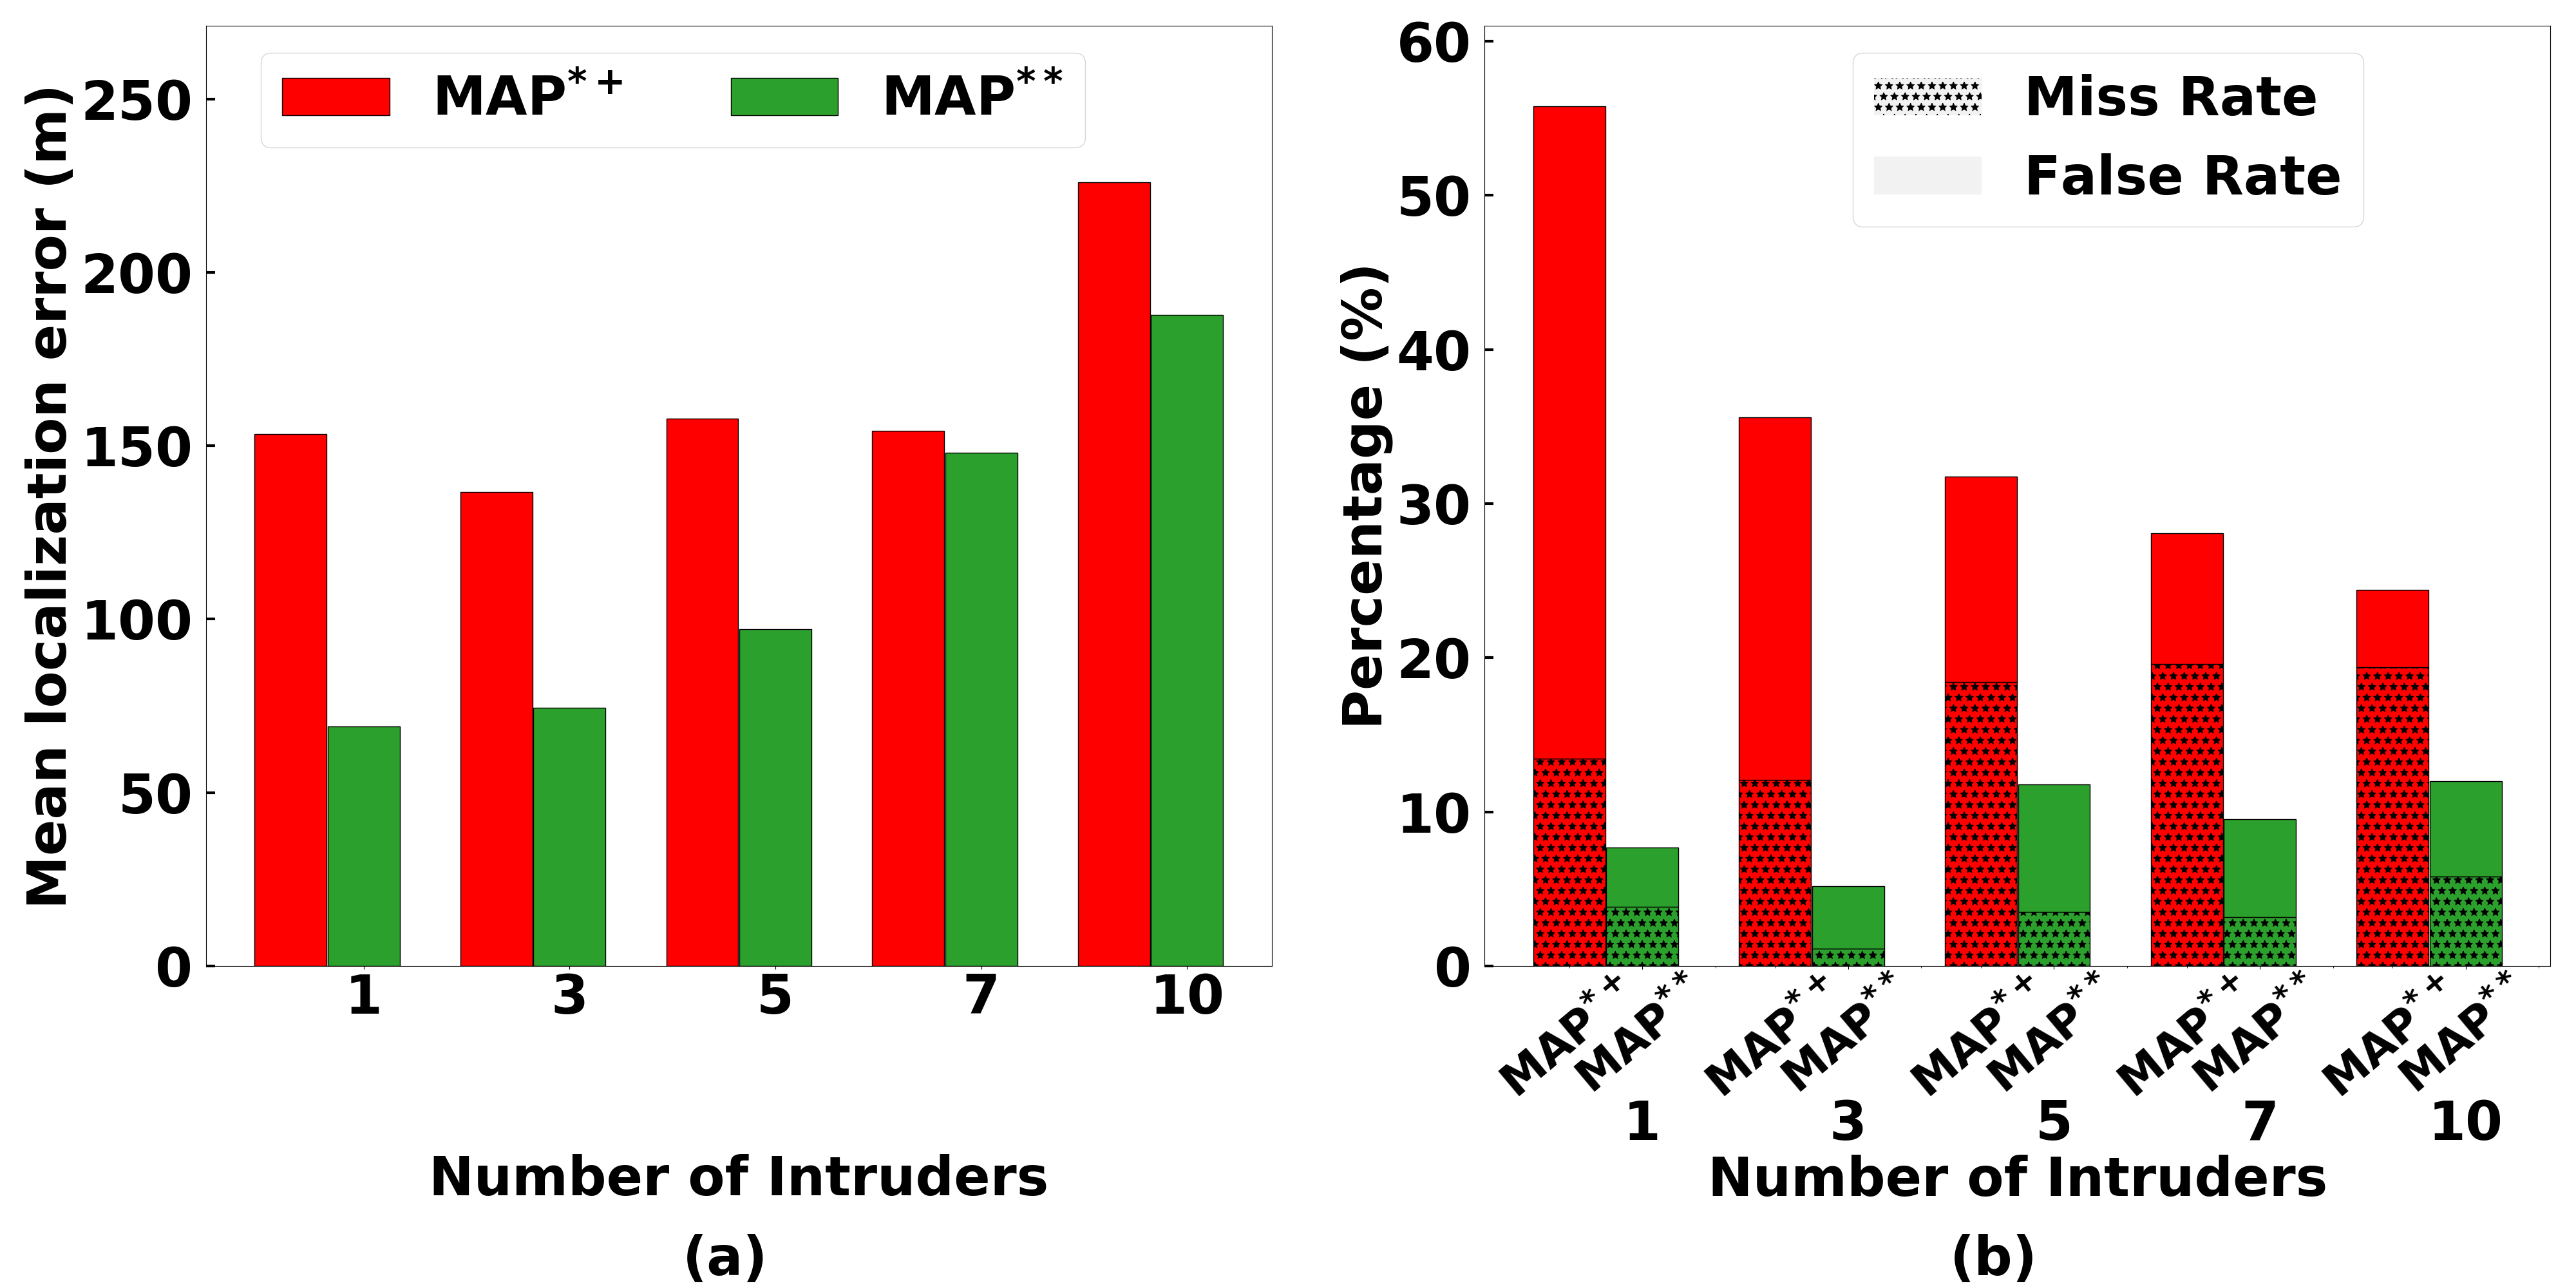
\includegraphics[width=0.8\textwidth]{chapters/ipsn/figures/splat-vary-numauthorized.png}
	\caption{Localization performance of \ouralgos and \ouralgoss in large-scale simulations with authorized users present, for varying number of intruders}
	\label{fig:shared-spectrum}
\end{figure}

\section{Testbed Implementation}
\label{sec:testbed}

In this section, we implement our techniques over commodity devices
and evaluate them over two small-scale testbeds---one indoor and one
outdoor.  Outdoor environment is a realistic setting for our target
application of shared spectrum systems, while the indoor environment
provides more challenging signal attenuation characteristics due to
walls and other obstacles.

\para{Sensor and Transmitters Used.}  Our low-cost (sub \$100, see~\cite{pam19-lowcostsensing} for a measurement study of low-cost spectrum sensors)
sensing device  is composed of a single-board computer
Odroid-C2 with an RTL-SDR dongle that
connects to a dipole antenna. We deploy 18 of these sensing devices
in our indoor and outdoor testbeds and configure them for low gain.
%The RTL-SDR devices has a noise floor of \ble{-48dB.}
%%%%%
For transmitters/intruders, we use USRP B210 and HackRF devices
  powered by laptops; we place these on a cart for mobility. These
  transmitter devices are uncalibrated, and there is no way to assign a
  specific transmit power. However, they have a configurable parameter
  called {\em gain} which is almost perfectly correlated to power when
  the gain is in a specific range, i.e., when the transmitter's gain
  is increased by 1, the receiver's signal strength increases by
  1dB. We thus use the gain parameter to adjust transmit power in the
  USRP devices. For indoor experiments, the location is manually
  derived, while for outdoor experiments, we use GPS
  dongles connected to the laptops. For collecting sensor
  observations, we implemented a Python repository in Linux that
  measures spectrum in real time at 915MHz ISM band and 2.4Msps
  sample rate.  The repository collects I/Q samples fetched from the
  RTL-SDR dongle and computes the RSS value, then records the RSS along
  with timestamp and location.  These three pieces of information are
  sent to a server that runs the localization algorithms. 

\begin{figure}
	\centering
	\begin{subfigure}[t]{0.45\textwidth}
		\includegraphics[width=\textwidth]{chapters/ipsn/figures/indoor.jpg}
		\caption{Indoor lab environment}
	\end{subfigure}
	\qquad
	\hspace{-0.15in}
	\begin{subfigure}[t]{0,42\textwidth}
		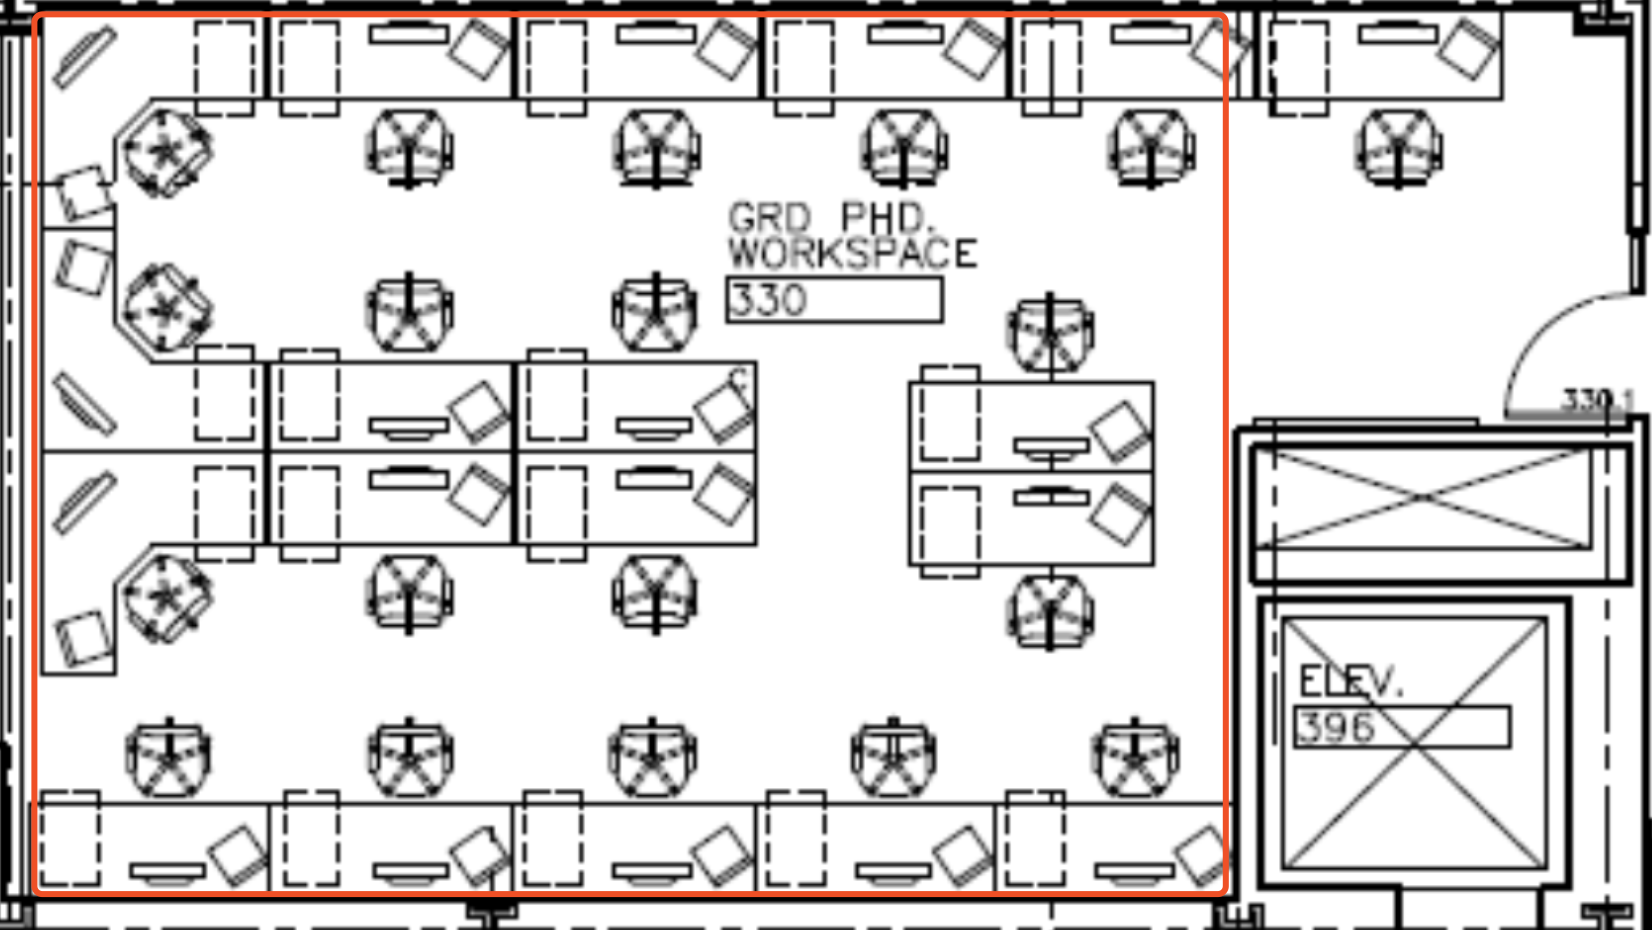
\includegraphics[width=\textwidth]{chapters/ipsn/figures/floor-plan.png}
		\caption{Floor plan}
	\end{subfigure}
	\caption{Indoor testbed. (a) Our lab used for the indoor testbed, (b) The lab's floor plan.}
	\label{fig:indoor}
\end{figure}

\begin{figure}
	\centering
	\begin{subfigure}[t]{0.585\textwidth}
		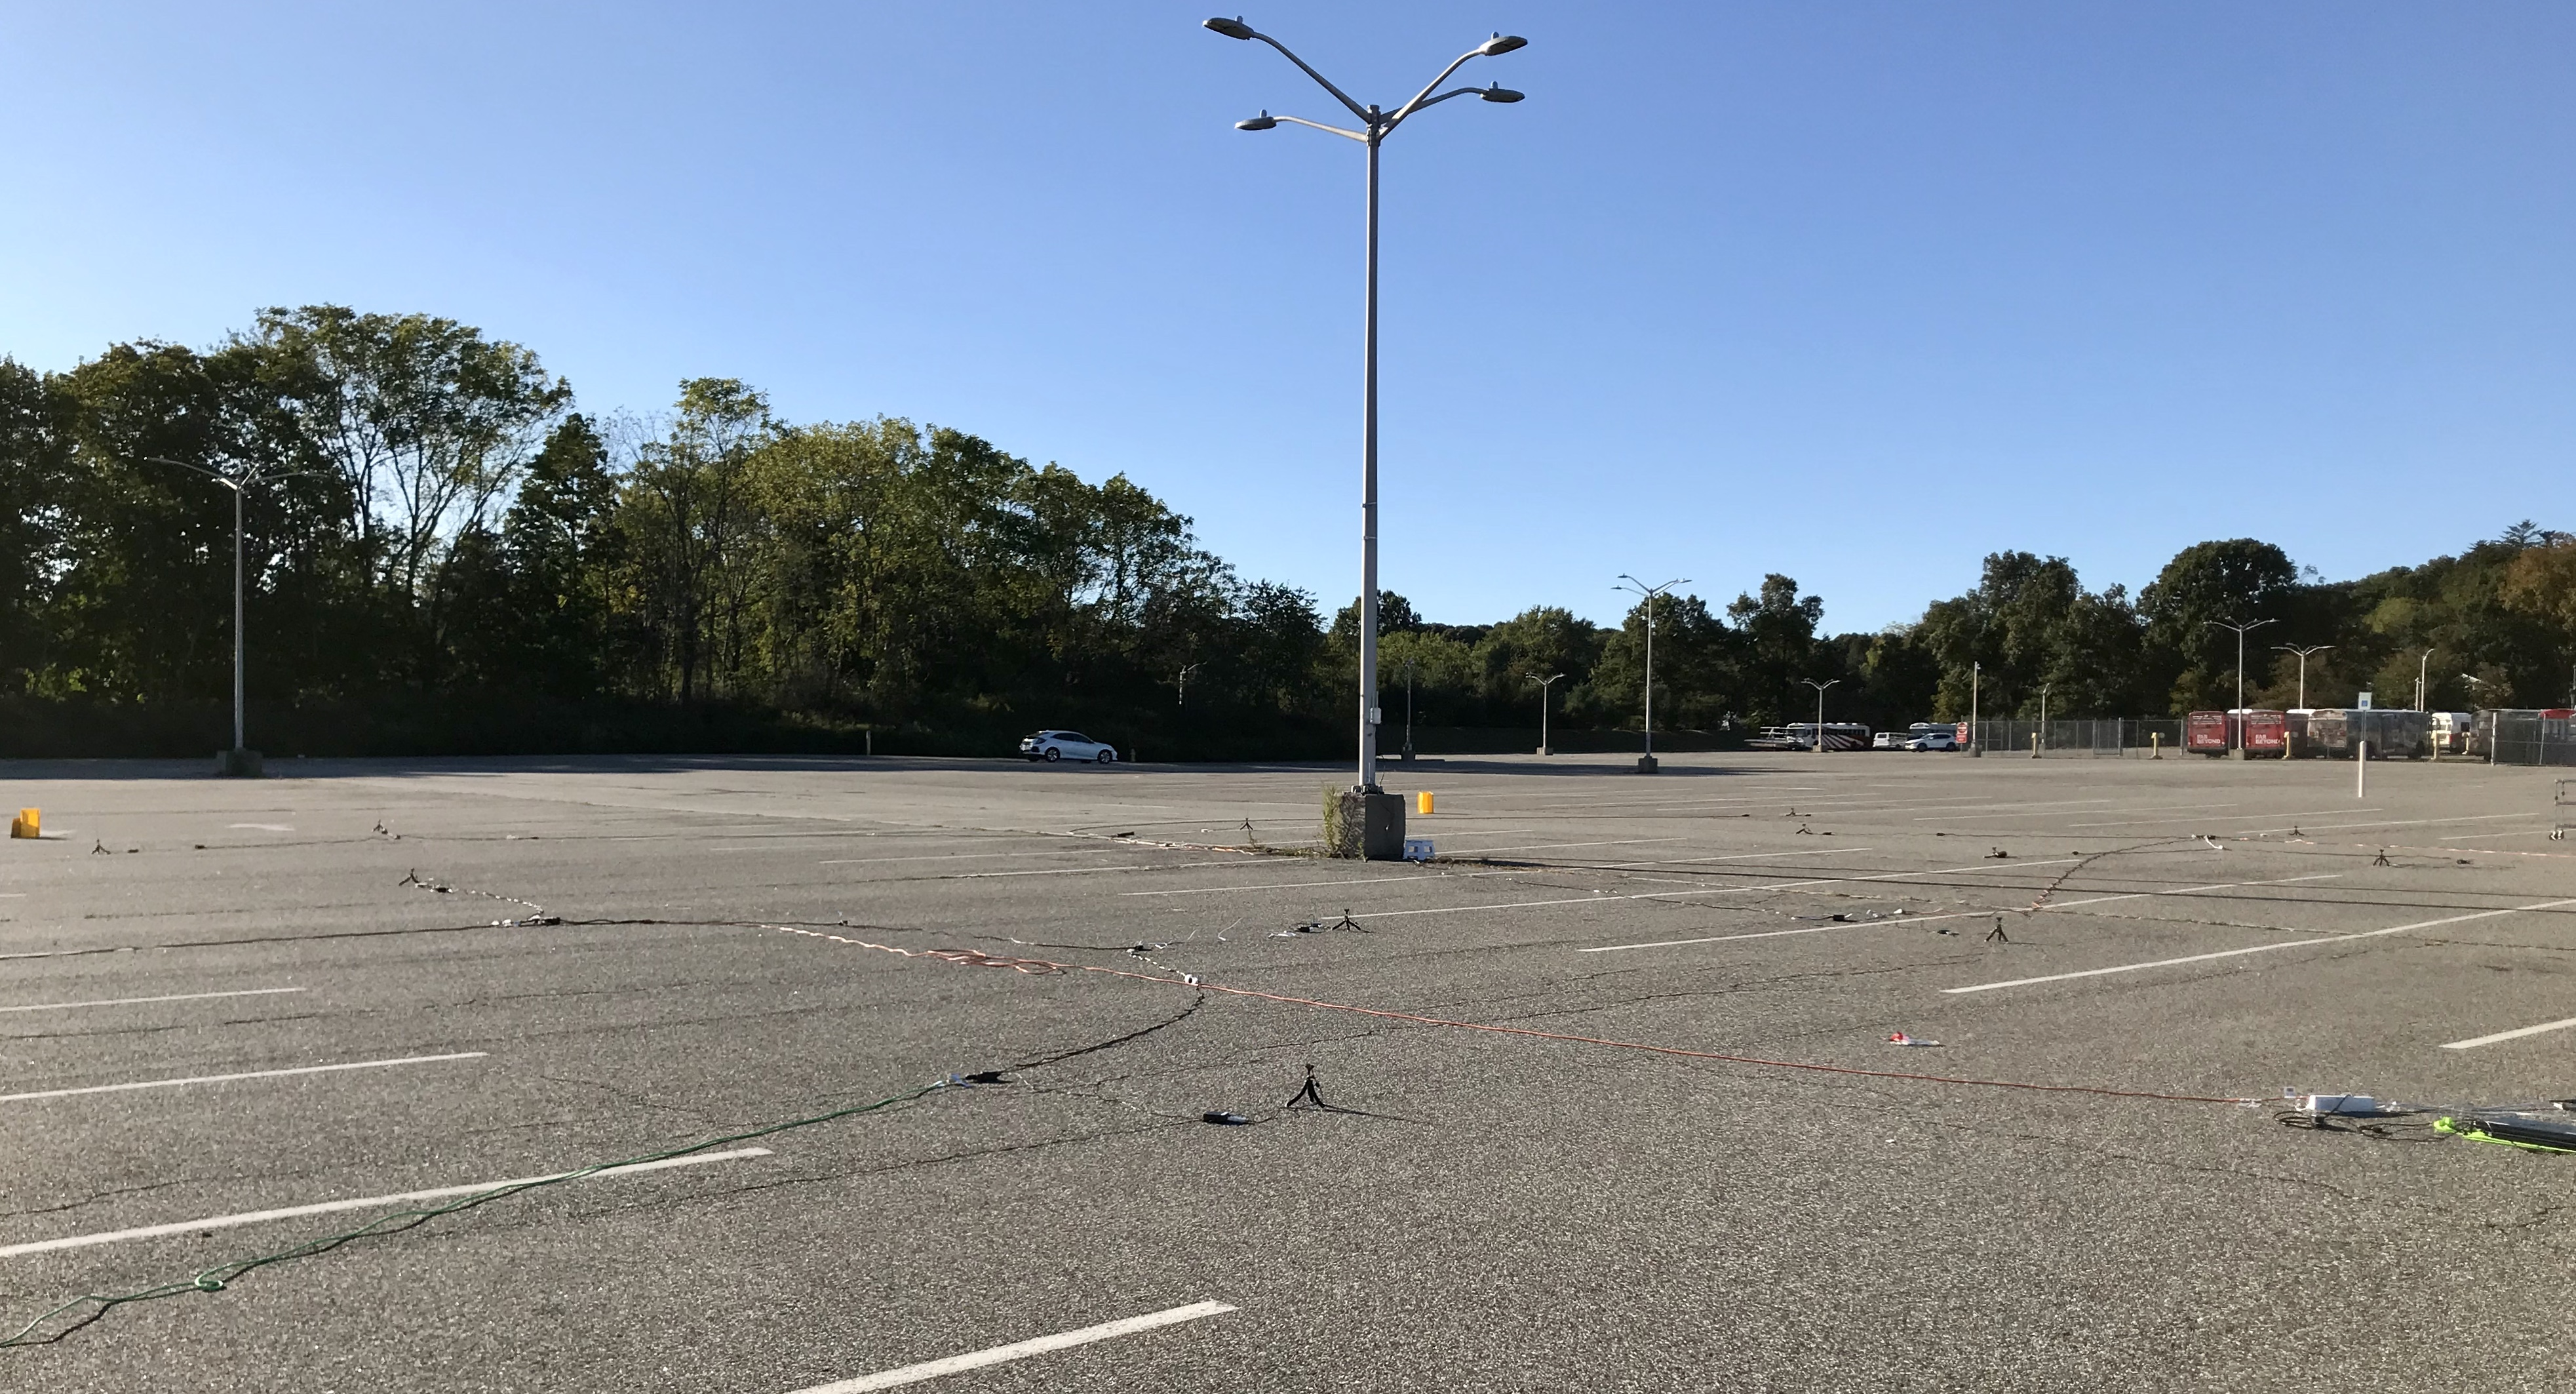
\includegraphics[width=\textwidth]{chapters/ipsn/figures/outdoor.jpg}
		\caption{Outdoor parking lot environment}
	\end{subfigure}
	\qquad
	\hspace{-0.15in}
	\begin{subfigure}[t]{0.33\textwidth}
		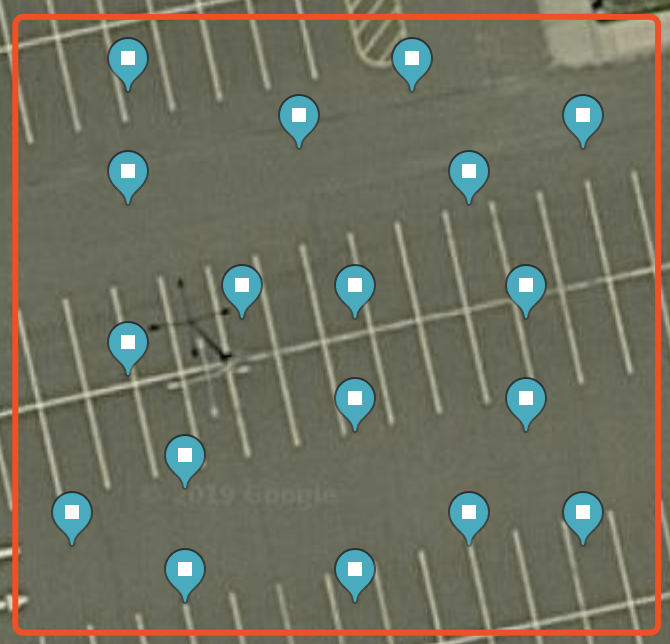
\includegraphics[width=\textwidth]{chapters/ipsn/figures/outdoor-sate.png}
		\caption{Satellite}
	\end{subfigure}
	\caption{Outdoor testbed. (a) Parking lot picture, (b)
          Satellite image of the parking lot; the red box is the area
          of the experiment, and the stars are the locations of
          sensing devices during evaluation.}
	\label{fig:outdoor}
\end{figure}

\para{Testbeds.} The {\bf indoor} testbed is built in a lab of our
Computer Science building.  Figure \ref{fig:indoor} depicts the lab
with its floor plan. The red box in the floor plan is the area where
experiments are conducted. The area is 9.6 $\times$ 7.2 $m^2$ (or 2177
square feet) large, with four rows of desks. The middle two rows
are separated by a wooden board. The area is imagined to be divided
into 48 grid cells each of size 1.2m $\times$ 1.2$m$, with the help of
ceiling tiles each of which is 0.6m $\times$ 0.6 $m$. 
%%%%
The {\bf outdoor} testbed is over an open space parking lot.  See
Figure~\ref{fig:outdoor}. The area is 32m $\times$ 32m. We divide the
area into 100 grid cells with each cell representing an area of 3.2m
$\times$ 3.2m. The GPS device returns the location in (latitude,
longitude) and the program converts it into coordinates. We use an
outdoor WiFi router and long power cords for network and electrical
connection respectively.
%%%%%%%
During the evaluation, the 18 sensing devices are placed on the ground
and are randomly spread out.


\para{Training.} In both the testbeds, for training (i.e.,
constructing non-interpolated PDs), we first pick 18 random grid cells
and place sensors in their approximate centers. Then, we manually move
the transmitter around in a cart through each of the grid cells. For
the USRP transmitter, we use a gain value of 45 in the indoor
environment and 58 in the outdoor testbed. We use a higher gain for
outdoors to allow the transmitter to have a larger transmission range
in a larger area.
%%%%%%
With each grid cell, the transmitter transmits from 3 to 4 different
points within each grid cell, and for each such location of the
transmitter, the sensors (at the 18 picked locations) gather tens of
signal strength readings. From these readings, we construct a Gaussian
probability distribution from each grid cell location of the
transmitter.
%%%%
More specifically, for a particular grid cell location of the
transmitter, we average over the readings from multiple TX positions
within that particular grid cell---this process of averaging different
positions of the TX inside a grid cell makes the Gaussian
distributions more robust to multipath fading and shadowing. The
overall training process takes an hour for indoors, and about two and
a half hours for outdoors.

\begin{figure}[ht]
	\centering
	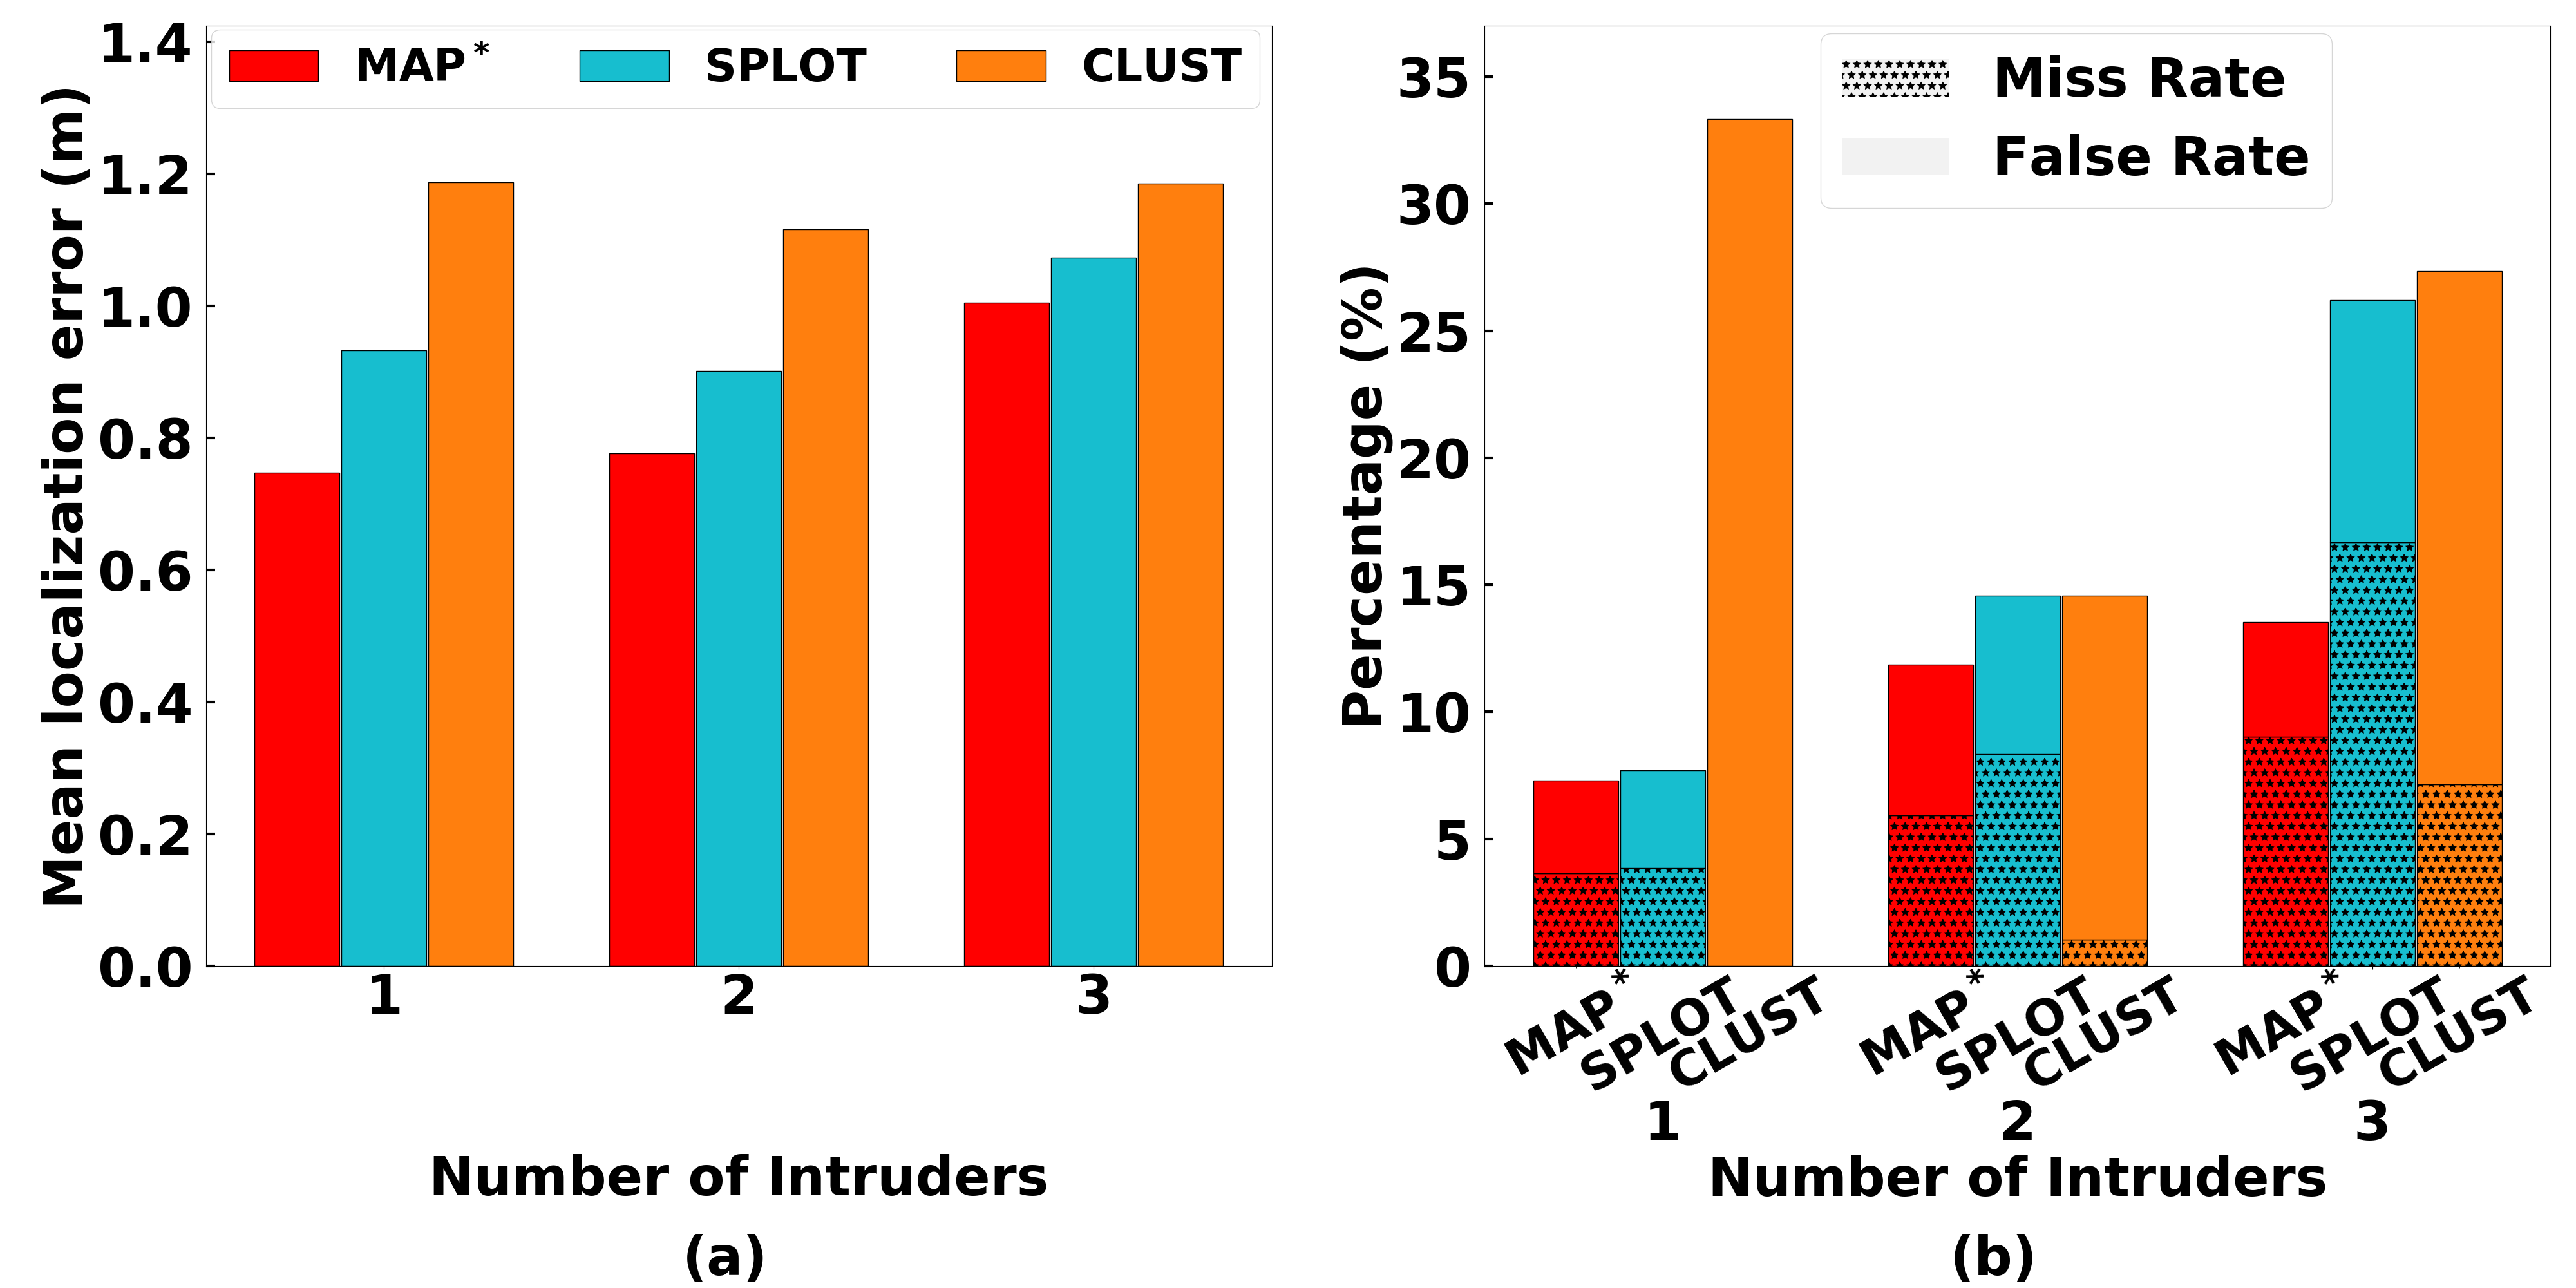
\includegraphics[width=0.8\textwidth]{chapters/ipsn/figures/indoor-error-missfalse.png}
	\caption{Localization performance of various algorithms in an indoor testbed}
	\label{fig:indoor-error-miss-false}
\end{figure}

\begin{figure}[ht]
	\centering
	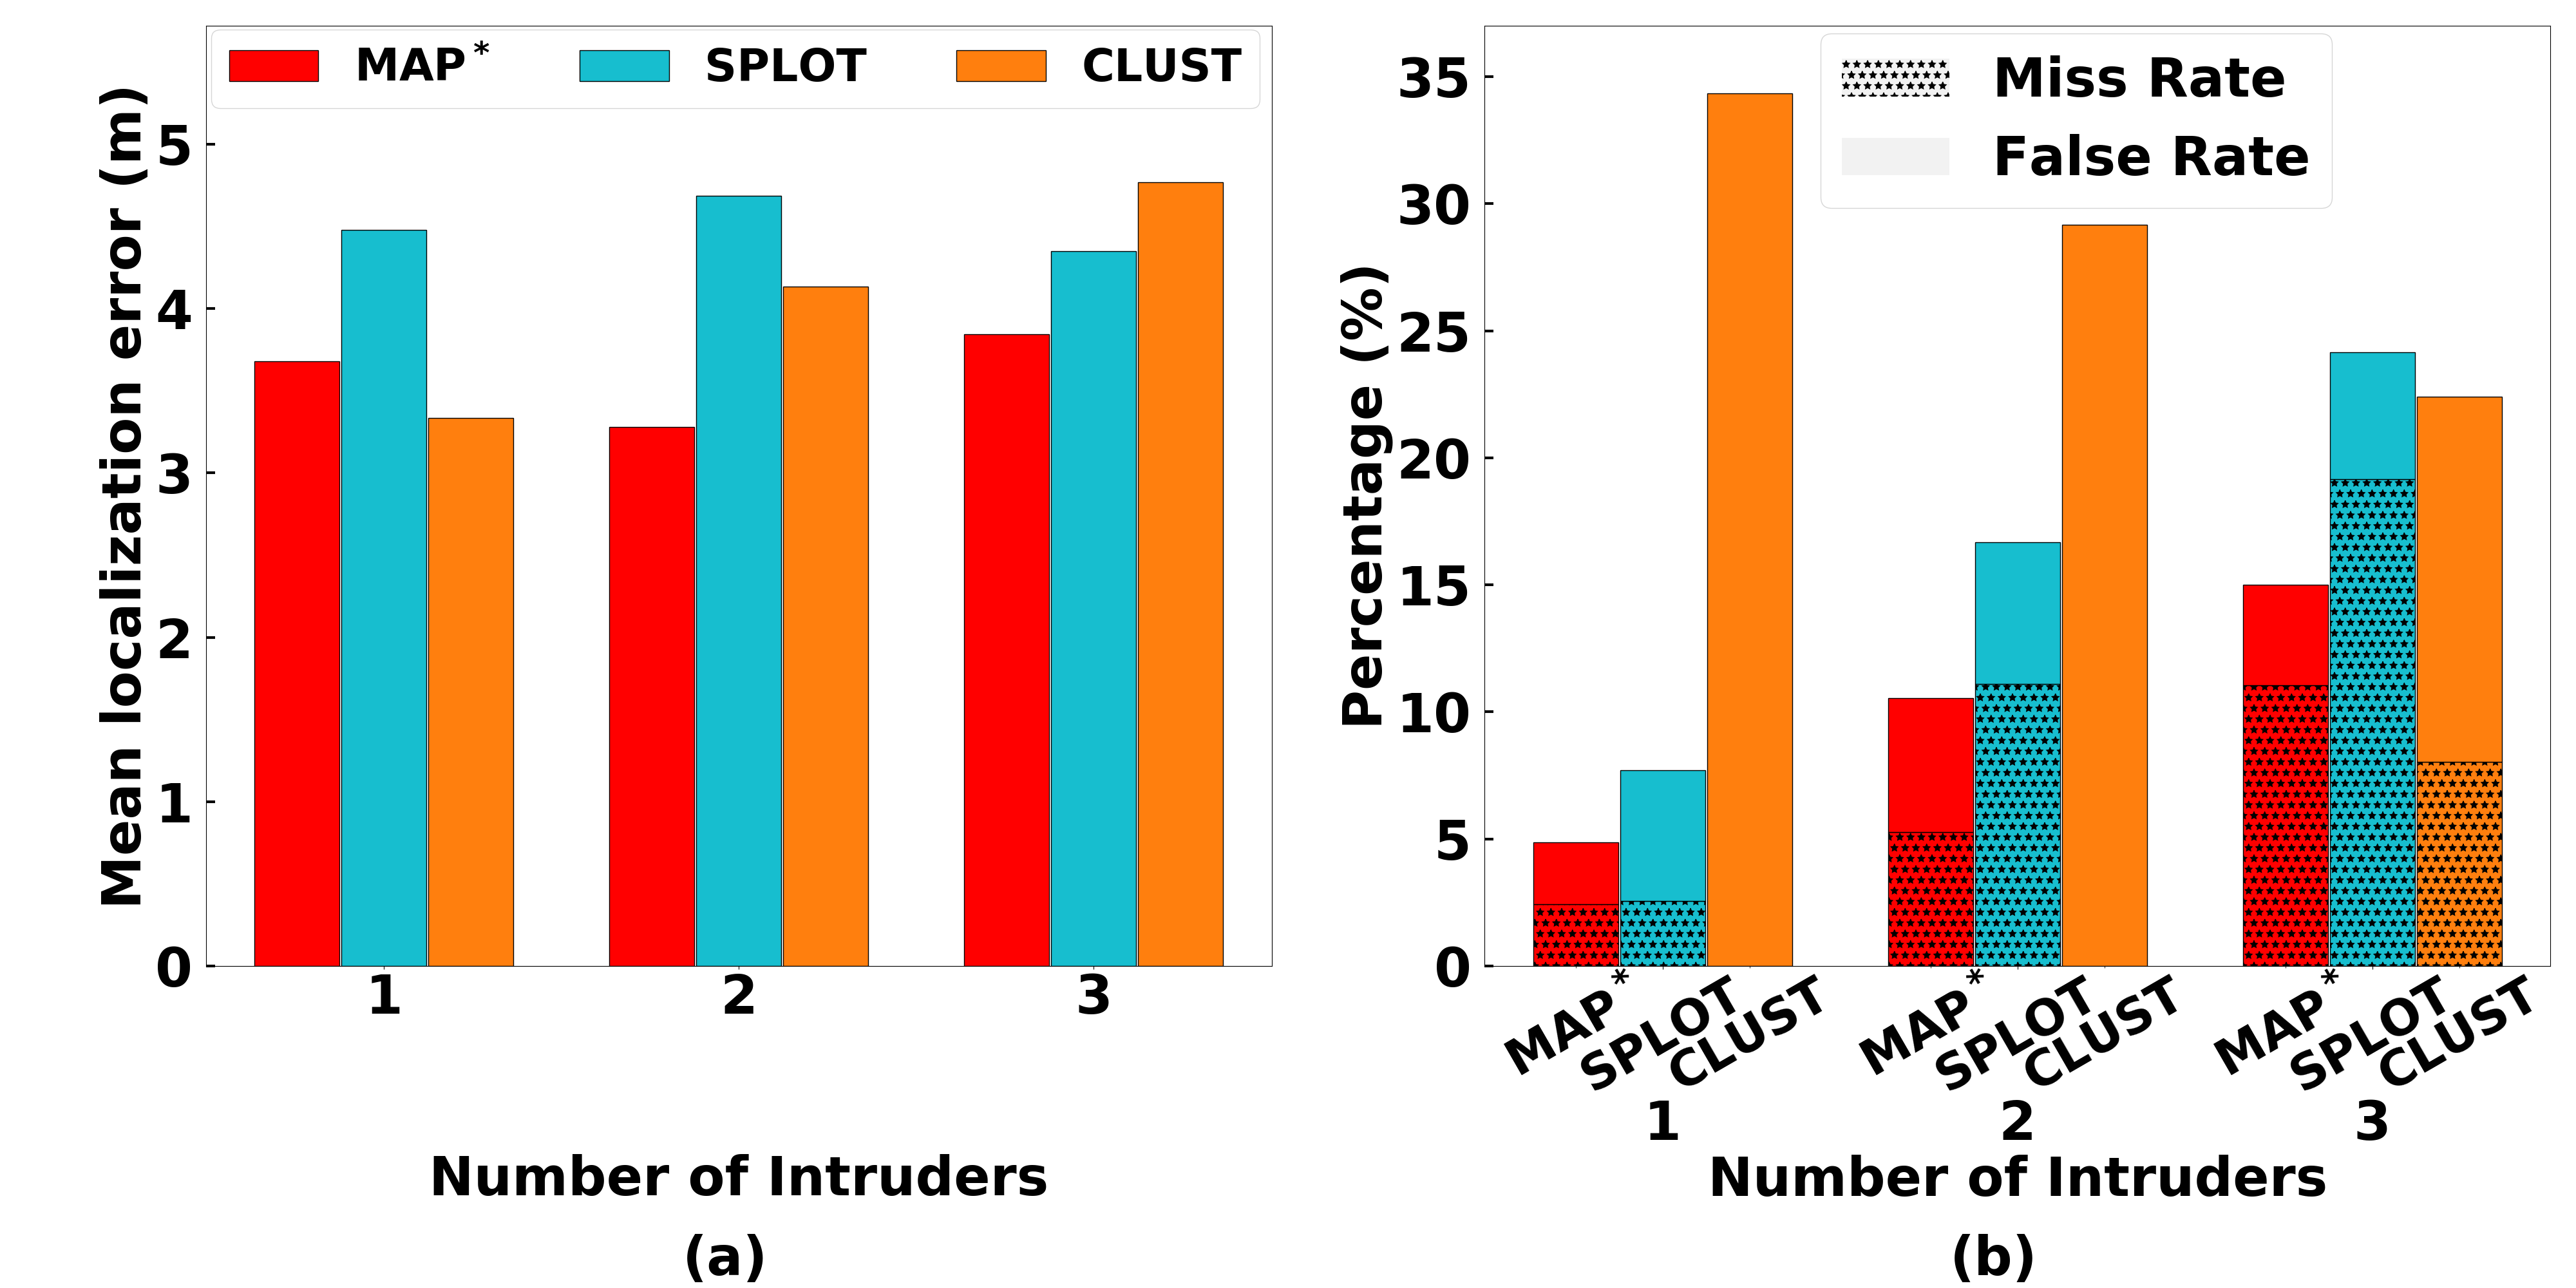
\includegraphics[width=0.8\textwidth]{chapters/ipsn/figures/outdoor-error-missfalse.png}
	\caption{Localization performance of various algorithms in an outdoor testbed}
	\label{fig:outdoor-error-miss-false}
\end{figure}

\para{Evaluation.}  For evaluation, in both testbeds, we place the 18
sensors at centers of grid cells that are randomly chosen and are
different from the cells chosen for the training above. The chosen
locations for the outdoor testbed are shown in
Fig.~\ref{fig:outdoor}(b). We choose the intruder's gain/power to be
in the range of [$\pstar-1, \pstar+1$], where $\pstar$ is the
gain/power used during the training phase as mentioned above.
%%%%%
Roughly half of our experiments involve close-by (in the same or
adjacent grid cells) intruders. Localization is done on a laptop which
listens to HTTP requests containing the sensors' observations. 

\subsection{Results}




\para{Localization Metrics.}
Figure~\ref{fig:indoor-error-miss-false}-\ref{fig:outdoor-error-miss-false}
show the localization results for the indoor and outdoor testbeds
respectively. Overall, the results indicate that \ouralgo performs the
best across all metrics, with the overall performance gap between
\ouralgo and \splot increasing with the increase in number of
intruders. When the number of intruders is 3, the performance of
\splot is significantly worse than \ouralgo due to a
significantly higher (84\% for indoors and 53\% for outdoors) sum of miss and false-alarm rates and 43\% higher localization error.
%%%%
The \cl algorithm generally performs the worst, but its
performance doesn't have a strong correlation with the increase in the
number of intruders; recall that \cl is given the range of number of
intruders as an extra piece of information compared to the other
algorithms.  In terms of absolute performance, we see that the
localization error of \ouralgo is roughly around 1 or less grid cell,
and the sum of miss-rate and false-alarm is between 5-15\%.


\begin{table}[ht]
	\centering
	\caption{Interpolation Mean Absolute Error (MAE) and  Mean Error (ME) in dB for \idw and \ildw}
	\begin{tabular}{c | c c c c}
		\hline\hline
		& \idw & \ildw &  \idw & \ildw \\ 
		Environment & (MAE) & (MAE)  & (ME) &  (ME) \\
		\hline 
		Indoor &  2.6 & 1.7  &  1.7 & 0.25  \\
		Outdoor & 6.2 & 2.7 & 5.8 & 0.48  \\
		\hline %inserts single line
	\end{tabular}
	\label{tab:inter-error}	
\end{table}



\para{Interpolation Error.}
Table \ref{tab:inter-error} shows the
interpolation mean absolute error (MEA) as well as mean error (ME) of
\idw and \ildw when the transmitter and receiver are close by (i.e.,
within a distance of 3 grid cells). When the transmitter and receiver
are far away, the difference between \idw and \ildw is small and thus not
shown.  We see that when compared with \idw, our \ildw interpolation
scheme decreased the mean absolute error by 35 percent in the indoor
environment and 56 percent in the outdoor environment.  In terms of
mean error, \ildw reduced the error compared to \idw by as large as 86
percent and 92 percent respectively. This is because \idw
mostly tends to estimate the value to be larger than the ground truth,
while \ildw's estimates are more even across the ground truth.

\begin{table}[ht]
	\caption{Power Prediction Mean Absolute Error (MAE) and Mean Error (ME) in dB for indoor and outdoor testbed}
	\centering
	\begin{tabular}{c | c c c c}
		\hline\hline
		& Indoor & Outdoor & Indoor  & Outdoor  \\
		\# Intruder  & (MAE)   &    (MAE)   &  (ME)  &   (ME)     \\
		\hline
		1 & 0.34 & 0.50 & -0.02 &  0.02 \\ 
		2 & 0.57 & 0.63  &  0.10 & 0.54\\
		3 & 0.77 & 0.90 & 0.49 & 0.76\\
		\hline %inserts single line
	\end{tabular}
	\label{table:power-error}
\end{table}

\para{Intruder Power.}  Table ~\ref{table:power-error} shows the errors in the predicted powers of
the intruders in \ouralgo. We see that the outdoors have a slightly
higher power prediction error, likely because of a larger number of
grid cells. We also note that with the increase in the number of
intruders, the error in predicted power increases.






\section{conclusions}

In this paper, we have developed an efficient Bayesian approach with a noval interpolation scheme to
localize multiple transmitters in presence of authorized users, and
demonstrate its superior power over large-scale simulations and smaller
scale indoor and outdoor testbeds.
%%%%%%
In our future work, we wish to extend our techniques to allow a
continuous location domain and design methods to further minimize
training cost. In addition, we will consider alternate signal
measurements such as angle-of-arrival (AoA).





\section*{Acknowledgments}

The work is supported by NSF grants CNS-1642965 and CNS-1815306. 
Thanks to Salman Qavi and Jayesh Ranjan for their help during the testbed.
Also thanks to Samir Das, Petar Djuric and Peter Milder for providing advice during group meetings.




\chapter[\small{DeepMTL: Deep Learning Based Multiple Transmitter Localization and\\Power Estimation}]{DeepMTL: Deep Learning Based Multiple Transmitter Localization and Power Estimation}
\label{chap:wowmom-pmc}

In this paper, we address the problem of Multiple Transmitter Localization (\mtl).
\mtl is to determine the
locations of potential multiple transmitters in a field, based on readings from a distributed set of sensors.
In contrast to the widely studied single transmitter localization problem, the \mtl problem has only been studied recently in a few works.
\mtl is of great significance in many applications wherein intruders
may be present. E.g., in shared spectrum systems, detection of unauthorized transmitters and estimating their power are imperative to 
efficient utilization of the shared spectrum.
	
In this paper, we present \our, a novel deep learning approach to address the \mtl problem.  
In particular, we frame
\mtl as a sequence of two steps, each of which is a computer vision problem: image-to-image translation and object detection. 
The first step of image-to-image translation essentially maps an input image representing sensor readings to an 
image representing the distribution of transmitter locations, and the second object detection step derives precise
locations of transmitters from the image of transmitter distributions.
%%%%%%%%%%%%%%%%%%%
For the first step, we design our learning model \imgimg, while for the second step, we customize a 
state-of-the-art object detection model \yolocust. 
%%%%%%%%%
Using  \our as a building block, we also develop techniques to estimate transmit power of the localized transmitters.
%%%%%%%%
We demonstrate the effectiveness of our approach
via extensive large-scale simulations and show that our approach outperforms the previous approaches 
significantly (by 50\% or more) in performance metrics including localization error, miss rate, and false alarm rate. 
Our method also incurs a very small latency.
We evaluate our techniques over a small-scale area with real testbed data and the testbed results align with the simulation results.

\section{Introduction}
\label{sec:intro}

The RF spectrum is a limited natural resource in great demand due to the
unabated increase in mobile (and hence, wireless) data
consumption~\cite{andrews2014will,sigcomm21-5G}.
In 2020, the U.S. FCC moves to free up 100 MHz of previously military occupied mid-band spectrum in the 3.45-3.55 GHz band for paving the way for 5G development. 
Also, the research and industry communities have been addressing this capacity crunch via the development of {\em shared spectrum}.
Spectrum sharing is the simultaneous usage of a specific frequency band in a specific geographical area and time by a number of independent entities where harmful electromagnetic interference is mitigated through agreement (i.e., policy, protocol)~\cite{dod20-spectrum}. 
Spectrum sharing techniques are also normally used in 5G networks to enhance spectrum efficiency~\cite{survey-specshare}.~However, protection of spectrum from unauthorized
users is important in maximizing spectrum utilization.

The increasing affordability of the software-defined radio (SDR)
technologies makes the shared spectrum particularly prone to
unauthorized usage or security attacks. With easy access to SDR
devices (e.g. HackRF, USRP), it is easy for selfish users to transmit data
on a shared spectrum without any authorization and potentially causing
harmful interference to the incumbent users.  Such illegal spectrum
usage could also happen as a result of infiltration of computer viruses
or malware on SDR devices.~\cite{survey-specshare} depicts three cases of spectrum attack.
As the fundamental objective behind such
shared spectrum paradigms is to maximize spectrum utilization, the
viability of such systems depends on the ability to effectively guard
the shared spectrum against unauthorized usage.  The current
mechanisms however to locate such unauthorized users (intruders) are
human-intensive and time-consuming, involving the FCC enforcement bureau
which detects violations via complaints and manual
investigation~\cite{mobicom17-splot}. 
Motivated by the above, we seek an effective
technique that is able to accurately localize multiple simultaneous
intruders (transmitters). Below, we describe the multiple transmitter localization problem.

%%% Multi-tx and challenges.
\para{Multiple Transmitter Localization (\mtl).}  \eat{Localization of
unauthorized users in a shared spectrum system essentially boils down to localizing transmitters/intruders in a given area under a shared spectrum system.}
The transmitter localization problem has been well studied, but most of the focus has been on localizing a {\em single} transmitter at a time. 
However, it is important to localize multiple transmitters simultaneously to effectively guard a shared spectrum
system. E.g., a malware or virus-based attachment could simultaneously 
cause many devices to violate spectrum allocation rules; spectrum
jamming attacks would typically involve multiple transmitters. More
importantly, a technique limited by the localization of a single intruder
could then be easily circumvented by an offender by using multiple
devices. The key challenge in solving the multiple transmitter localization (\mtl) 
problem comes from the fact that
the deployed sensor would receive only a {\em sum} of the signals from multiple transmitters, and separating the signals may be impossible. 
\eat{In
addition, the other challenge that \mtl in the context of shared
spectrum system poses is the presence of authorized users---e.g., the
incumbent users and the dynamic set of secondary users that have been
allocated spectrum by the manager.}
% To the best our knowledge, no prior localization work has considered the presence of authorized users.

%%%% SPLOT and shortcomings.
\softpara{Prior Works.}
The \mtl problem has been recently addressed in a few prior works, among which \splot~\cite{mobicom17-splot}, \map~\cite{ipsn20-mtl}, and 
\deeptx~\cite{icccn20-deeptxfinder} are the most 
prominent. \splot essentially decomposes the \mtl
problem to multiple single-transmitter localization problems based on
the sensors with the highest power readings in a
neighborhood. However, their technique implicitly assumes a propagation model, and
thus, may not work effectively in areas with complex propagation
characteristics, and it is not effective in the case of transmitters
being located close by (a key challenging scenario for \mtl problem).
Our recent work \map solves the \mtl problem using a 
hypothesis-driven Bayesian approach; in particular, it uses prior training in the form of distributions
of sensor readings for various transmitter locations, and uses the training data to determine
the most likely configuration (i.e., transmitters' locations and powers) for a 
given vector of sensor readings. 
However, to circumvent the high computational cost of a pure Bayesian approach,
\map uses a divide and conquer heuristic which results in somewhat 
high number of misses and false alarms while still incurring high
latency. 
%%%%%%%%%%%
\deeptx uses a CNN-based learning model approach; 
however, they use a separate CNN model for a specific number of transmitters
and thus may incur high model complexity and training cost while also limiting the number 
of transmitters that can be localized.
In our evaluations, we compare our work with each of the above approaches.
%In this approach, like ours, a model is trained, which later is used to predict the configuration of the transmitters the best based on sensors received power.
%\eat{In our evaluation, we
%  have compared our technique with theirs and one other approach.}
%%\blue{Our localization approach belongs to the fingerprinting~\cite{infocom00-radar} category.}

\begin{figure}[t]
\centering
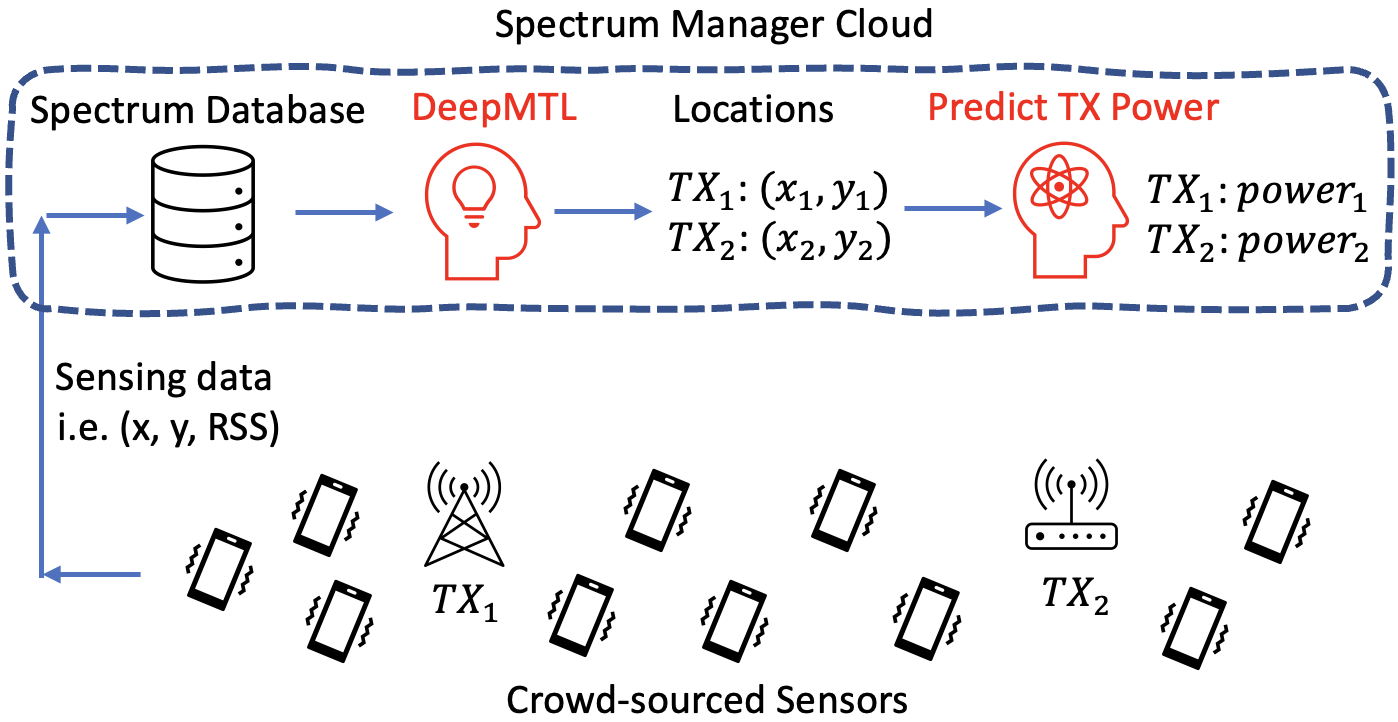
\includegraphics[width=0.9\textwidth]{chapters/wowmom-pmc/figures/architecture.png}
\caption{Multiple transmitter localization using a distributed set of sensors. Sensing data is uploaded to a spectrum manager server in the cloud. \our is a deep learning approach to multiple transmitter localization which helps protect 
spectrum against unauthorized usage. After that, prediction of transmission powers happens using \our as a building block.}
\label{fig:illustration}
\end{figure}

%%%%%%%WHAT we DO.
\para{\our: Our Two-Step Approach.}  As in prior
works~\cite{mobicom17-splot,chakraborty2017specsense}, we assume a
crowdsourced sensing architecture (See Fig.~\ref{fig:illustration}) wherein relatively low-cost spectrum
sensors are available for gathering signal strength in the form of received power.
We use a convolutional neural network (CNN) based approach
to solve the \mtl problem. In particular, we frame
\mtl as a sequence of two steps: image-to-image translation and object detection, each of which
is solved using a trained CNN model. 
The first step of image-to-image translation maps an input image representing sensor readings to an 
image representing the distribution of transmitter locations, and the second object detection step derives precise
locations of transmitters from the image of transmitter distributions.
We name our \mtl approach as \our.
%%%%%%%%%%%%%%%%%%%

\softpara{Motivation.}
Our overall approach and its various aspects are motivated by the following considerations. 
{\bf First}, we use a learning-based strategy to 
preclude assuming a propagation model~\cite{mobicom17-splot} or conducting surveys of sensors reading distributions~\cite{ipsn20-mtl}.
Assumption of propagation model suffers from the fact that 
even sophisticated propagation models yield unsatisfactory accuracy and thus lead to degraded performance.
Among all learning-based strategies, deep learning can implicitly capture the environment characteristics (e.g., objects, walls, landscape) in the neural network layers' weights learned through the training of the data~\cite{mobicom20-deeploc}.
Even though a learning-based approach incurs a one-time high training cost,
it generally incurs minimal latency during inference, which is an important consideration for our \mtl problem.
The intruder detection should incur minimal latency to be effective.
{\bf Second}, the geographical nature of the \mtl problem suggests that convolutional neural networks (CNNs) are 
well-suited for efficient
learning of the desired function. In particular, the features of the \mtl problem can be
represented in an image (2D matrix) corresponding to their geographic locations, which can be fed as an input
to an appropriate CNN model which can leverage the spatial correlation among the input features 
to facilitate efficient learning. 
{\bf Lastly,} we use a two-step architecture to  facilitate efficient training by essentially
providing an additional intermediate image. 
In particular,  we are able to map each step to well-studied standard computer vision problems, allowing us to build upon known techniques. 

\para{Overall Contributions.}  The goal of our work is to develop an
efficient technique for accurate localization of simultaneously
present multiple transmitters/intruders. We also extend our technique to address various
extensions such as power estimation and the presence of authorized users. Overall, we make the following 
contributions.
\begin{enumerate}
\item
For the \mtl problem, we develop a novel two-step CNN-based approach called \our approach. 
For the first step of image-to-image translation, we develop a CNN model that translates an image representing the sensor readings into an intermediate image that encodes distributions of transmitter locations (Section \ref{sec:translate}). 
%%%%%%%
For the second step of mapping transmitter distributions to precision locations via object detection,
we customize the well-known  object detection method YOLOv3 (Section \ref{sec:detect}).

\item
For localization of transmitters in presence of authorized users, we 
augment the \our model by adding a pre-processing step based on a 
CNN-model that first reduces the 
sensor readings by the power received from the authorized users (Section \ref{sec:authorized}).

\item
To estimate transmit power of the intruders, we augment our \our model
with a power-estimation CNN-model which iteratively estimates the power of transmitters
in sub-areas (Section \ref{sec:power}).

\item
We evaluate our techniques via large-scale simulations as well as a small-scale testbed data and demonstrate their effectiveness and superior
performance compared to the prior works (Section \ref{sec:evaluation}).
\end{enumerate}

A preliminary version of this paper appeared at IEEE WoWMoM 2021~\cite{wowmom21}.

\eat{ 
\item Why two steps? We could directly go for sensor readings to TX locations .. we help the model by adding an intermediate step.
    
    We aim to fulfill the task by introducing two CNN models. One for converting sensors reading image to TXs image and another one to localize existing TXs.
    The effectiveness of learning-based object localization techniques, in our case, relies on the fact that how accurate and close our representing input (image) is to real objects image. So, we decide, first, to convert sensors reading image to TXs' (real target objects) image via our first CNN model. This way, we block any possible anomaly to propagate to the next CNN model which is a deeper model.
    Another benefit of this approach is to use the output of the first CNN model in non-learning algorithms that may need less training samples (faster) but have probably less accuracy.

}




\eat{
As CNN has proved its powerful strength mostly in Computer Vision and specially in localizing objects in images, sensors being crowd-sourced in a topological area reporting received power from multiple transmitters, representing them as an image will be a natural choice.
The second benefit of training a model is we do not need any knowledge about the signal propagation characteristic.
% Our motivation for using a \map-based
% approach is multifold: First, with sufficient training data, \map is
% known to deliver optimal classification accuracy for the MTL problem.
% Second, the \map approach doesn't assume any propagation model and
% thus works for arbitrary signal propagation characteristics.
Third, relating sensor readings to a TX's image (where TXs are represented as objects based on their location and power) allows us to also estimate the intruder's transmit power, which can be very useful in some applications, e.g., where the penalty is
proportional to the extent of violation.
\blue{Lastly and most importantly,
it naturally extends to being able to handle a presence of an evolving
set of authorized users.}
}


%train convolution  to design a CNN-based model that efficiently localize intruders based on sensors reading. Our approach is a deep learning technique in which sensors reading is represented as CNN-friendly input, an image.


% hypothesis-driven Bayesian approach,
% viz.\ {\em maximum a posteriori} (\map) approach, wherein each
% hypothesis is a configuration (i.e.  a combination of $\langle
% location, power \rangle$ pair) of the potential intruders, and the
% goal is to determine the hypothesis that best explains the sensor
% observations. This determination is done based on the distributions
% (gathered during a training phase) of sensor observations for each
% hypothesis.
%%%%%%%%%%%%


%%%%% MOTIVATION.



% \blue{\emph{Novel Interpolation}. The \map framework requires prior
% training to build probability distributions (PDs) of sensor
% observations for each hypothesis.
% In our work, we reduce the number of PDs to be constructed via a novel
% interpolation scheme suited to our unique setting, and evaluate the
% impact of reduced training on the localization accuracy.}








% 	The RF spectrum is a limited natural resource in great demand. 
	
% 	(Can include a piece of news on US releasing spectrum for 5G from military)
	
% 		%Previous methods using some machine learning techniques are either %not accurate, slow, or not able to localize transmitters close by. 
% 	%Recent work uses deep learning to solve the multiple transmitter %localization problem.
% 	%We utilize the power of convolution neural networks and push the \mtl %solution to the next level.
	
	
% \cite{ipsn20-mtl}
% \cite{mobicom20-deeploc}
% \cite{icccn20-deeptxfinder}
\section{Background, \mtl Problem and Our Approach}
\label{sec:problem}
\label{sec:prob-def}

In this section, we describe the background of the shared spectrum systems,
formulate the \mtl problem, then describe our methodology. 

\para{Shared Spectrum System.} In a shared spectrum paradigm, the
spectrum is shared among licensed users (primary users, PUs) and
unlicensed users (secondary users, SUs) in such a way that the
transmission from secondaries does not interfere with that of the
primaries (or secondaries from a higher-tier, in case of a multi-tier
shared spectrum system). In some shared spectrum systems,
the location and transmit power of the primary users may be
unavailable, as is the case with military or navy radars in the CBRS band.
%%%%%
Such sharing of spectrum is generally orchestrated by a centralized
entity called {\em spectrum manager}, such as a spectrum
database in TV white
space~\cite{sas-paper} or a central spectrum access system in
the CBRS 3.5GHz shared band~\cite{milind2015dyspan}. The spectrum
manager allocates spectrum to requesting secondaries (i.e., permission
to transmit up to a certain transmit power at their location) appropriately
so as to avoid interference to primaries.
%%%%%%%%%%%%
Users that transmit without explicit permission are referred to as 
unauthorized users or {\em intruders}; the \mtl problem is to essentially
localize such intruders. 

\para{\mtl Problem.}  Consider a geographic
area with a shared spectrum. Without loss of generality, we assume a
single wireless frequency\footnote{To avoid confusion with image channels, we use {\em wireless frequency} instead of the perhaps more appropriate {\em wireless channel} term.} throughout this paper\footnote{Multiple wireless frequencies can be handled independently. 
Note that if we assume the wireless propagation characteristics to be similar for different frequencies, then we do not need to train different models for each of them. Our localization techniques would still work
for scenarios wherein the intruders may change their transmit frequencies dynamically.}.
For localization of intruders, we assume
available crowdsourced sensors that can observe received signal in the wireless frequency of interest, and compute (total) received signal strength (RSS).
RSS can be measured using low-cost sensors and has been shown to achieve good accuracy for single-transmitter localization~\cite{infocom00-radar}.
In the related work Section~\ref{sec:wowmom-related}, we will discuss signal metrics other than RSS, such as AoA, ToA, etc.~At any instant, there may be a set of intruders
present in the area with each intruder at a certain location transmitting
with a certain power which may be different for different intruders.
%%%%%%%%%%%%%%%%%%%%%%%%%%%

The \mtl problem is to determine the set of intruders with their
locations at each instant of time, based on the set of sensor
observations at that instant. 
%%%%%
For the main 
\mtl problem, we assume that there are no primary or authorized users, and thus, assume that the
sensor readings represent aggregate received power from the transmitters we
wish to localize.
However, in Section \ref{sec:authorized}, we investigate the more general \mtl problem where the background primary and/or secondary users may also be present.

\begin{figure*}
    \centering
    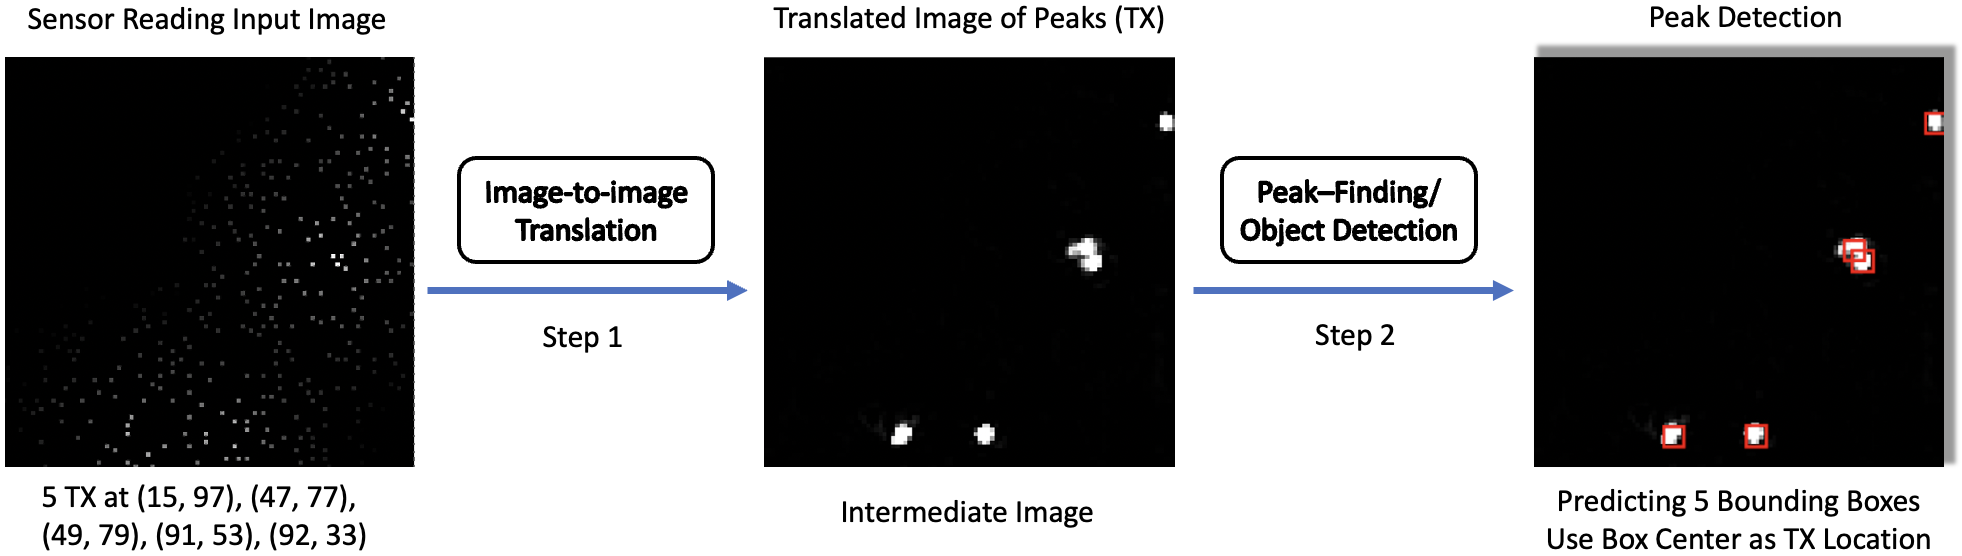
\includegraphics[width=\textwidth]{chapters/wowmom-pmc/figures/two-step-idea.png}
    \caption{The overall two-step CNN architecture of the \our model. The first step is the \imgimg, whose higher idea is to translate the input image of sensor readings to the image of peaks where each peak implies a transmitter. The \imgimg architecture is illustrated in Fig.~\ref{fig:part1}. The second step is \yolocust, a customized version of YOLOv3, to perform object/peak detection in the output image of the first step. This step returns the precise location coordinates of TX. The \yolocust architecture is illustrated in Fig.~\ref{fig:yolo}. A zoom-in of the peak detection result of the second step is in Fig.~\ref{fig:peaks}.}
    \label{fig:overall}
\end{figure*}

\para{\bf Our Approach.}
In our context, each sensor communicates its observation to a centralized spectrum 
manager which then runs localization algorithms to localize any potential (multiple) transmitters. 
%%%%%%%%%%%%%%%%%%%%%
We design and implement a novel two-step localization algorithm named \our, as illustrated in Fig.~\ref{fig:overall}, based on CNN models. 
The first step (Section \ref{sec:translate}) is a four-layer image-to-image translation CNN model that is trained
to translate an input image representing sensor readings to an image of 
transmitters' locations distributions. Each distribution of a transmitter can be visualized as a mountain with a peak, so we name this model \imgimg.
The second step (Section \ref{sec:detect}), called \yolocust, is a customized object-detection method build upon YOLOv3\cite{yolov3} which localize the objects/peaks in the translated image.
%%%%%%%%%%%%%%%%%%
The high-level motivation behind our two-step design is to frame the overall \mtl
problem in terms of well-studied learning problem(s). 
The two steps facilitate efficient learning of the models by supplying an intermediate image with the training samples. 
%With this design, we fix the drawback in~\cite{icccn20-deeptxfinder} that needs to train a large number of models and it is way more accurate. We elaborate the step 1 in Section \ref{sec:translate} and step 2 in Section \ref{sec:detect}.
%}

\section{\our Step 1: Sensor Readings to TX Location Distributions}
\label{sec:translate}

In this section, we present the first step of our overall approach to the \mtl problem, i.e., 
the image-to-image translation step which translates/transforms the sensor reading to distributions
of TX locations. Here, we first create a grayscale image to represent the input sensor readings;
this image encodes both the sensors' RSS readings and the sensors' physical location. We then train and use
a convolutional neural network (CNN) model to transform this input image
to an output image which represents the distribution of TX locations. Pixels in the output image that have higher values will have a higher chance of having a TX being present at that location. 
 
\para{Input/Output Image Sizes and Tiling Approach for Large Areas.}
We need to represent data by images of certain sizes.
Typically, an image should be a size of a few hundred pixels by a few hundred pixels, since a thousand pixels by thousand pixels images will consume too much GPU memory.
In this paper, we pick $100\times 100$ as the size for both our input and output images in the first image-to-image translation step.
Given an area that we want to monitor and a $100\times100$ size image, we will know how large an area a pixel will represent and we call it a pixel subarea.
%%%%%%%%
A large pixel subarea could certainly lead to high localization errors, due
to very coarse granularity. We can address this by using a ``tiling"
technique, wherein we divide the given area into tiles, then represent each 
tile by $100\times100$ size image and use our localization techniques in the tile.
We can do some post-processing to handle cross-tiling issues (e.g., \cite{icccn20-deeptxfinder} uses overlapping tiles and employs a voting scheme inside the overlapping tile area).
 
\eat{\blue{For our \our, each pixel represents a $10m\times 10m$ area. Since \our input image is of size $100\times 100$, the whole input image represents a $1000m\times1000m$ area. 
To deal with a larger area, let's say $10000m\times 10000m$ area, two simple methods are: increase the input image size to $1000\times 1000$; 
Or let each pixel represent a $100m\times 100m$ area.
The first method requires redesigning \our (changing layer hyperparameter etc.).
Note that the input image size is usually in the range of lower hundreds. 
For example, $224\times 224$ is used by ResNet \cite{resnet} and $416\times 416$ is used by YOLO. 
$1000\times 1000$ is generally speaking too big as it will consume too much GPU memory.
Also, a pixel representing a larger area means coarser granularity and lower accuracy.
A reasonable approach will be keeping the \our as it is, and use a ``sliding window" like method, i.e. slide the \our 100 times (10 rows, 10 columns) to cover the $10000m\times10000m$ area.
\deeptx\cite{icccn20-deeptxfinder} is using this idea and they name it a tile-based approach.
To deal with smaller areas, we can fill the rest of the area with noise floor values. 
By filling, we can make smaller images fit into the $100\times100$ input size requirement of \imgimg.
In the following subsection \ref{subsec:ipsn}, we demonstrate how we generate a $100\times 100$ size image from a $10\times 10$ size grid in real-world testbed data.}
}
%\todo[inline]{Is this 10m x 10m ?}


%%%%%%%%%%%%%%%%%%%%%%%%%%%%%%%%%%%%%%%%%%%

\subsection{Input Image Representing Sensors' Readings}

We localize transmitters based on observations from a set of sensors, i.e. solve the \mtl problem assuming only intruders.
%Below, we present details on how to represent the information gathered from the set of crowd-sourced sensors.
%\para{Sensor Observations' Matrix to Image.} 
The input of the localization method is sensor observations. 
Here, an {\em observation} at a sensor is the received power (RSS, in decibels) over a time window of a certain duration, in the frequency of interest (we assume only one wireless frequency). 
RSS is computed using FFT over the I/Q samples collected in a time window. More specifically, in our evaluations, we use a Python API \cite{psd} that computes the power spectral density from a sequence of signal data (I/Q samples), and then, we choose the RSS at the frequency of interest.
%%%%
\begin{figure}[t]
    \centering
    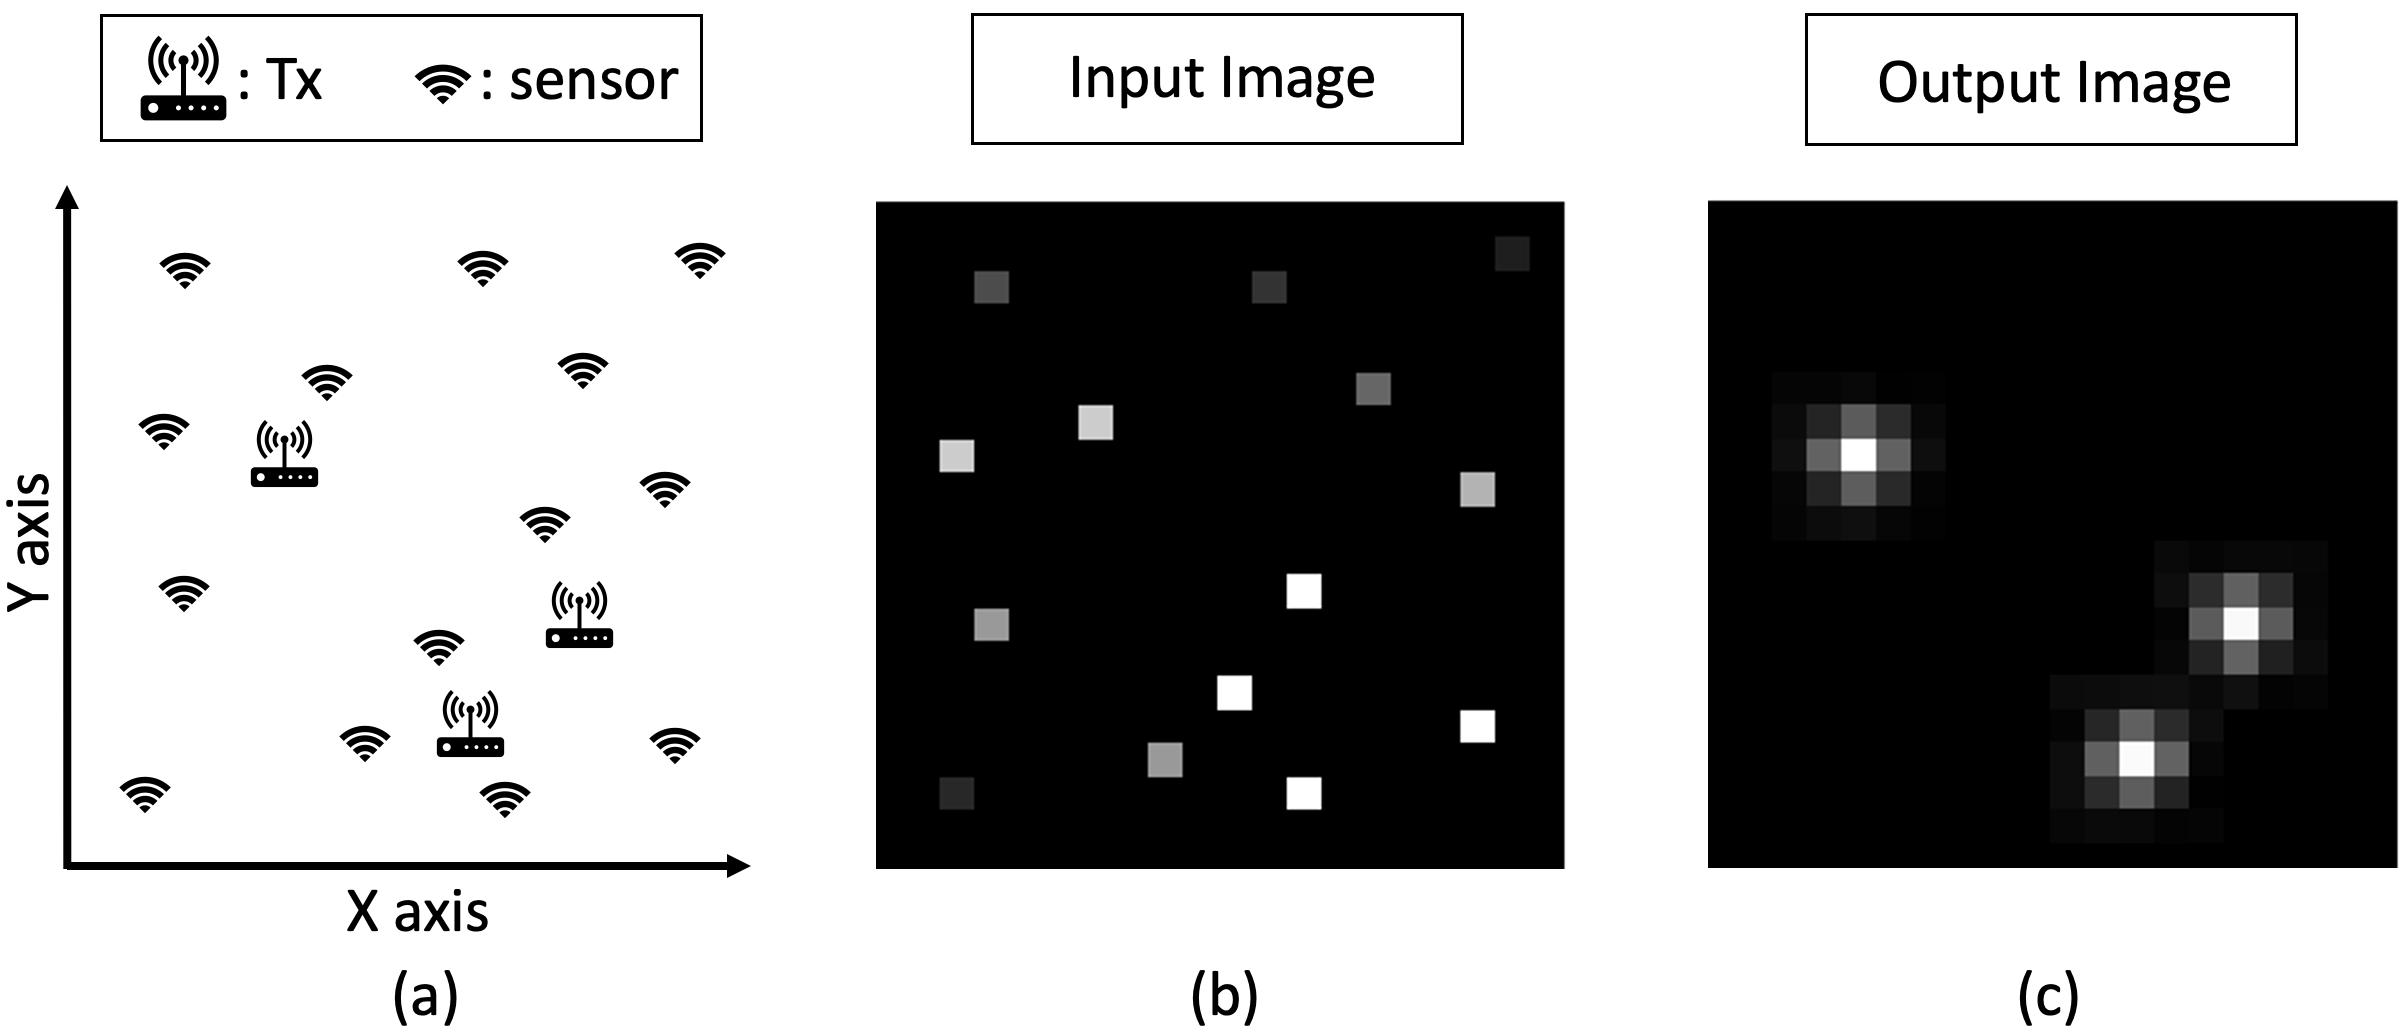
\includegraphics[width=0.75\textwidth]{chapters/wowmom-pmc/figures/input-output.png}
    \caption{Illustration of \our first step's input and output images. (a) Area with distributed sensors and transmitters to be localized. (b) Input image representing the sensor readings (RSS) and locations. (c) Output Image, where we put a 2D Gaussian distribution with its ``peak" at the transmitter's location.}
    \label{fig:input}
\end{figure}
Different than~\cite{mobicom17-splot,ipsn20-mtl}, we represent the sensor information, i.e.,
their locations and observations, in a 2D input image.
%%%%%%%%%%%%%%%%%%%%%%%%%%%%%
We use a 2D grayscale image, and let us denote it $\mx$. The pixel \mxij denotes the observation of the sensor at the grid cell whose index is $(i, j)$. For example, $\mx_{10, 20}=-50$ denotes there is a sensor at coordinate $(10, 20)$ with an RSS reading of $-50$ dB. 
If there is no sensor at location $(i, j)$, we assign the noise floor $\nf$ (i.e. -80 dB) value to \mxij.
Note that the above pixel values (representing the sensor observations) are not the standard
image pixel values that lie in the [0, 255] range.
Also, since the pathloss computed by propagation models during simulations could be real numbers, the sensor observation values could be real numbers. 
So we use a 2D matrix with real numbers instead of an image object.

Before passing this sensor reading image as input to our CNN model, we do a normalization step; we first subtract the $\nf$ from each value and then divide it by $-\nf$/2.
Let $\mxx$ denote the 2D matrix after the normalization of $\mx$. 
The value $\mxxij$ will be zero at locations without sensors, and \mxxij will be a positive real number (in most cases, less than two) for locations with sensors. E.g., if $\mx_{10, 20}=-50$, then the 
$\mxx_{10, 20}$ equals to $(-50- (-80)) / 40) = 0.75$.
Fig.~\ref{fig:input}~(b) shows how a matrix is used to represent the input information that contains both the RSS and the spatial location of the distributed sensors in an area that exists 14 sensors in Fig.~\ref{fig:input}(a).
%%%%%%%%


%%%%%%%%%%%%%%%%%
% \blue{
% When the input is an image, the door of a type of deep learning networks, convolutional neural network (CNN), opens to us. 
% Thus we are able to borrow brilliant new methodologies from the computer vision community.
% }



%%%%%%%%%%%%%%%%%%%%%%%%%%%%%%%%%%%%%%%5

\subsection{Output Image Representing TX locations' Distributions}
\label{subsec:imgimg_output_image}
We now focus on designing the output image to represent the distribution of TX locations; 
the output image is essentially the ``label" assigned to each input image that guides the training of the CNN model. 
Fig.~\ref{fig:input}(c) illustrates the output image of the image-to-image translation step in Fig.~\ref{fig:input}(a) that contains three transmitters.

A straightforward representation that represents the TXs with locations is to just
use an array of $(x, y)$ elements where each $(x, y)$ element is the location of a 
transmitter, as in~\cite{icccn20-deeptxfinder}.
%%%%%%%%%%%%%%
However, this simple representation is less conducive to efficient model learning,
as the representation moves away from spatial representation (by representing locations 
as positions in the image) to direct representation of locations by coordinate values.
E.g., in~\cite{icccn20-deeptxfinder}'s CNN-based approach to \mtl problem, the authors
assume a maximum number $N$ of transmitters and train as many as $N+2$ different CNN models
and thus, limiting the overall solution to the pre-defined maximum number of 
transmitters.
%%%%%%%%%%%%%%
Instead, in our approach, we facilitate the learning of the overall model, by solving the
\mtl problem in two steps, and in this step of translating sensors' reading
to transmitter locations' distributions, we represent the output also as an image.
This approach allows us to use a spatial learning model (e.g. CNN) for the second step too, and preclude
use of regression or fully-connected layers in the first step. 

Inspired by recent work on wireless localization problem~\cite{mobicom20-deeploc} that represents the input and output as images, we represent our output of the first step as an image as well.
The output image is a grayscale image implemented as a 2D matrix with real numbers. 
In the output image, we use 25 ($5\times 5$) pixel values to represent the presence of a transmitter. 
It is desirable to use an odd side length square (e.g., $3\times 3$, $5\times5$, $7\times 7$) for symmetry. 
For a $100\times 100$ size input we use, while $3\times3$ gives too little information for a transmitter and $7\times 7$ generates too many overlaps for close by transmitters, $5\times 5$ is the sweet spot.
Other pixels far away from any transmitter are zero-valued.
%%%%%%%%%%%%%%%%%%%%
Among multiple potential ways to represent a transmitter presence by a number of pixels, we found
that using a 2D Gaussian distribution around the pixel of TX location, as shown in Fig.~\ref{fig:input}(c), yields the best model performance.
Thus, a geographic area with multiple transmitters present is represented by a grayscale image with multiple Gaussian distributions, with each Gaussian distribution's peak inside the pixel corresponding to transmitter's location. 
%%%%%%%%%%%%%%%%%%%%
Based on preliminary performance
tests, we pick the amplitude of the 2D Gaussian peak to 10, the standard deviation to 0.9, and located the center of the distribution at the location of each transmitter.
Note that the location of the TX is in continuous domain and usually not at the center of the grid cell.
%To represent off-center location of a transmitter within the grid cell, we offset the intensity value at each pixel by the distance between the actual location of the transmitter and the grid cell's center.

% \red{Need very precise details. 
% How is the continuous location of TX represented? How many pixels do you use to represent a single TX? How is the power being represented? Note that the transmitter's location is in the continuous domain. 
% So the center of the Gaussian peak is also in the continuous domain, and is usually not precisely located at the center of a pixel. 
% But each pixel is represented as the center of the pixel. 
% Thus the pixel's center value in the 2D Gaussian function will be assigned to the pixel.}

%%%%%%%%%%%%%%%%%%%%%%%%%%%%%%%%%%%%%%%
%%%%%%%%%%%%%%%%%%%%%%%%%%%%%%%%%%%%%%%%

\begin{figure}
    \centering
    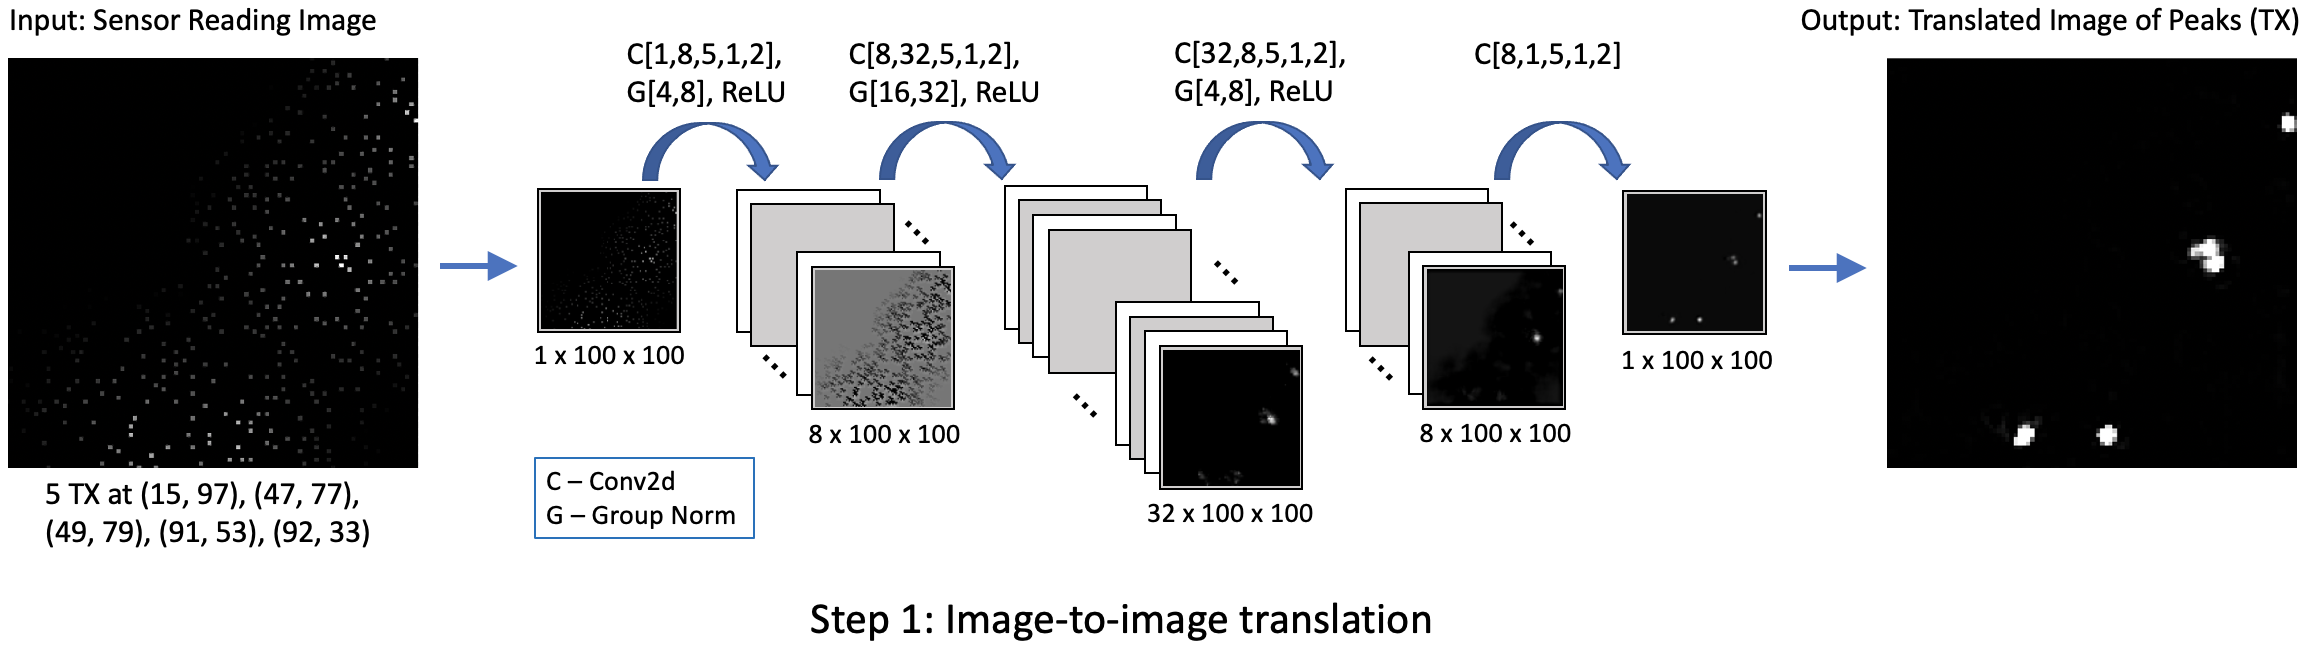
\includegraphics[width=\textwidth]{chapters/wowmom-pmc/figures/part1.png}
    \caption{Architecture of the first step CNN, a four layer image-to-image translation model (\imgimg). The figure displays how the data volume flows through the various convolutional layers. C stands for Conv2d, and for each Conv2d layer, the five values shown are [number of input channels, number of output channels, kernel size, stride, padding]. G stands for group normalization, and, for each group normalization, the two values shown are [number of groups, number of channels]. See~\S\ref{sec:translate} for details.}
    \label{fig:part1}
\end{figure}


\subsection{Image-to-Image Translation: \imgimg CNN Model}
\label{subsec:img-translate}

At a higher level, we use a deep and spatial neural network, in particular a CNN, to learn the
approximation function that maps the input image (of sensor readings) to the output image (of Gaussian distributions for TX locations). We refer to this as the {\em image-to-image translation}
model. Our approach is inspired by the recent work~\cite{mobicom20-deeploc} that frames 
a different wireless localization problem as an image-to-image translation problem.
%%%%%%%
We incorporate the idea into our multiple transmitter localization problem and utilize recent advances in the computer vision area. 
Encoder-decoder based CNN models like U-Net~\cite{miccai15-unet} with down-sampling
and up-sampling convolutional layers have been successful in effectively learning image-to-image translation functions. However, in our setting, we observe that the usage of down-sampling layers (such as max-pooling) degrades the performance of the model, especially in the case when transmitters may be close to each other wherein the model is unable to distinguish the nearby transmitters and generate a single large distribution in the output image. To circumvent this, we avoid using any
down-sampling layers in our model and redesign the image-to-image translation model as described below.

% There are several \red{well-known} learning models that learn functions for image-to-image translation. 
% These image translation models can roughly be classified into two types\cite{img2img-survey}: encoder-decoder-based, such as U-Net~\cite{miccai15-unet}, and GAN-based\cite{nips14-gan}, such as pix2pix~\cite{cvpr17-pix2pix}. In general, GAN-based models 
% are more  complex than the encoder-decoder-based models, and \red{their goal is vastly different than ours .... some specific details as to why GAN-based are not relevant for us.} 
%%%%%%%%%%%%%
% For our context, wherein our target images are much simpler, we observe that the simple encoder-decoder image translation model is sufficient to solve our problem. 
%%%%%%%%%%%%%%%%%
% \red{Describe some high-level differences between GAN and encoder-decoder models, or at the very least, what the encoder-decoder model looks like.}
%%%%%%%%%%%%%%%%%%%%%%%
% We tried standard encoder-decoder model design strategies and \red{HG: The following sentences can not be understood, without more details on encoder-decoder modes.} skip connections like \cite{miccai15-unet}. But we found out that the down-sampling mechanisms such as max-pooling are losing the information and the skip connection are not enough to make up the information loss.

\para{\imgimg CNN Model}. 
We refer to our image-to-image translation CNN model as \imgimg, as it translates sensors' 
readings to ``peaks" with Gaussian distributions corresponding to transmitter locations.  
It has four \footnote{We observe that a four-layer lightweight and symmetric \imgimg  model produces good results and adding more layers gives marginal improvement.}
convolutional layers, as shown in Fig.~\ref{fig:overall}(a). 
We use an input size of $100\times100$. The number of convolutional filters are varying for
different layers, with up to 32 in one of the layers. 
%%%%%
We tried doubling the filter numbers at each layer, but it does not lead to significant 
improvement (it does yield a lower error, but the output image does not improve significantly
to impact the second step of our architecture). We use a kernel size of $5\times5$, a stride of 1, and a padding of 2.
This ensures that the dimensions do not decrease and all the pixels are treated 
uniformly, including the ones at the edge of the image.
With the above four convolutional layers, the receptive field~\cite{receptive-field} of each neuron in the output layer is $17\times17$.
Normalization layers can improve the learning process. We chose group normalization \cite{groupnorm} and put it after the first three convolutional layers. 
We compared group and batch normalization~\cite{batchnorm} methods in our context, and observed
better performance with the group normalization. 
For the activation layers, we select rectified linear unit (ReLU) and put it after the group normalization layers.

% \softpara{Derived Pixels in Higher Layers.} 
% We have four convolutional layers with kernel size of 5x5. 
% So a neuron on the first convolutional layer will have 
% 5x5 view of the input volume, and a neuron on the second convolutional layer will have a 5x5 view of the first convolutional layer and thus a 9x9 view of the input volume, and so on. Thus, a 
% a neuron on the forth convolutional layer (and also the output layer) 
% will have a 17x17 view of the input volume. So each single pixel 
% in the output image is derived from 17x17 pixels of the input image. \blue{Whats the point of talking about this? .}

\softpara{The Loss Function}. Our inputs ($X$) and output ($Y$) are images. We use L2 loss function which computes the mean squared error aggregated over individual pixels.
More formally, our loss function is  defined as:
\begin{equation}
 \frac{1}{N} \sum_{i}^{N} || \imgimg(X_i) - Y_i ||^2
 \label{equ:sen2peak_loss}
\end{equation}
where $N$ is the number of samples used in computing the loss, $|| \cdot ||^2$ is L2 loss function, $X_i$ and $Y_i$ are the $i_{th}$ sample's input and output images respectively, and $\imgimg(X_i)$ is the predicted output image corresponding to the input $X_i$. During training, we use 
Adam~\cite{kingma2017adam} as the optimizer that minimizes the loss function. We set the learning rate to 0.001 and the number of epochs to 20 and the model converges well.
% \red{more info about the training and testing such as normalization. HG: Not sure its needed.}
\section{\bf \our Step 2: TX Locations' Distributions to Precise Locations}
\label{sec:detect}

In this section, we present the second step of our overall localization approach. We refer to
this step as the {\em peak detection} step, as the goal is to detect the peaks within the 
Gaussian distributions in the input image (which is also the output image of the first step).
%%%%
The first step outputs an image that has multiple distributions (presumably, Gaussian), whose
peaks need to be interpreted as precise locations of the transmitters/intruders.
%%%%%%%%%%%%
As, our end goal is to determine the precise locations of the present transmitters, we develop techniques to detect peaks within  the output image of the first step. 
%%%%%%%%%%%%%%%%%%%%%%%
We propose two different strategies for the peak-detection task. The first strategy is a straightforward peak detection algorithm based on finding local maximal values, while the 
second strategy is based on framing the problem as an object detection task; for the second strategy, we utilize a widely used state-of-the-art computer vision model called YOLOv3~\cite{yolov3}.

\para{Simple Peak Detection Method.}
The simple and straightforward peak detection method is to designate pixels with
locally maximal values as peaks, subject to certain thresholds.
%%%%%%%%%
More formally, we use a threshold $x$ for a peak value, and also use a parameter $r$ to define a $r$-radius neighborhood of a pixel. 
Then, any pixel whose value is more than $x$ and is the maximum among all pixels with a $r$-radius neighborhood, is designated as a peak (transmitter location). 
We use $x=2$ and $r=3$, in our evaluations.
%%%%%%%%%%%%%
Note that each pixel represents a subarea; thus, a pixel designated as pixel only 
implies the transmitter location at the {\em center} of the corresponding subarea.
%%%%%%%
To localize the transmission more precisely with the pixel's subarea, we use a scheme that localizes the transmitter within the subarea by computing a weighted average of the peak pixel's coordinate and the peak's neighbor pixels' coordinates.
The weight of a pixel is the predicted pixel value itself from the first step \imgimg.
%%%%%%%%%%%%%%%%%%%%%
We refer to the above simple approach for the second-step of \our as \simpeak.

\begin{figure}
	\centering
	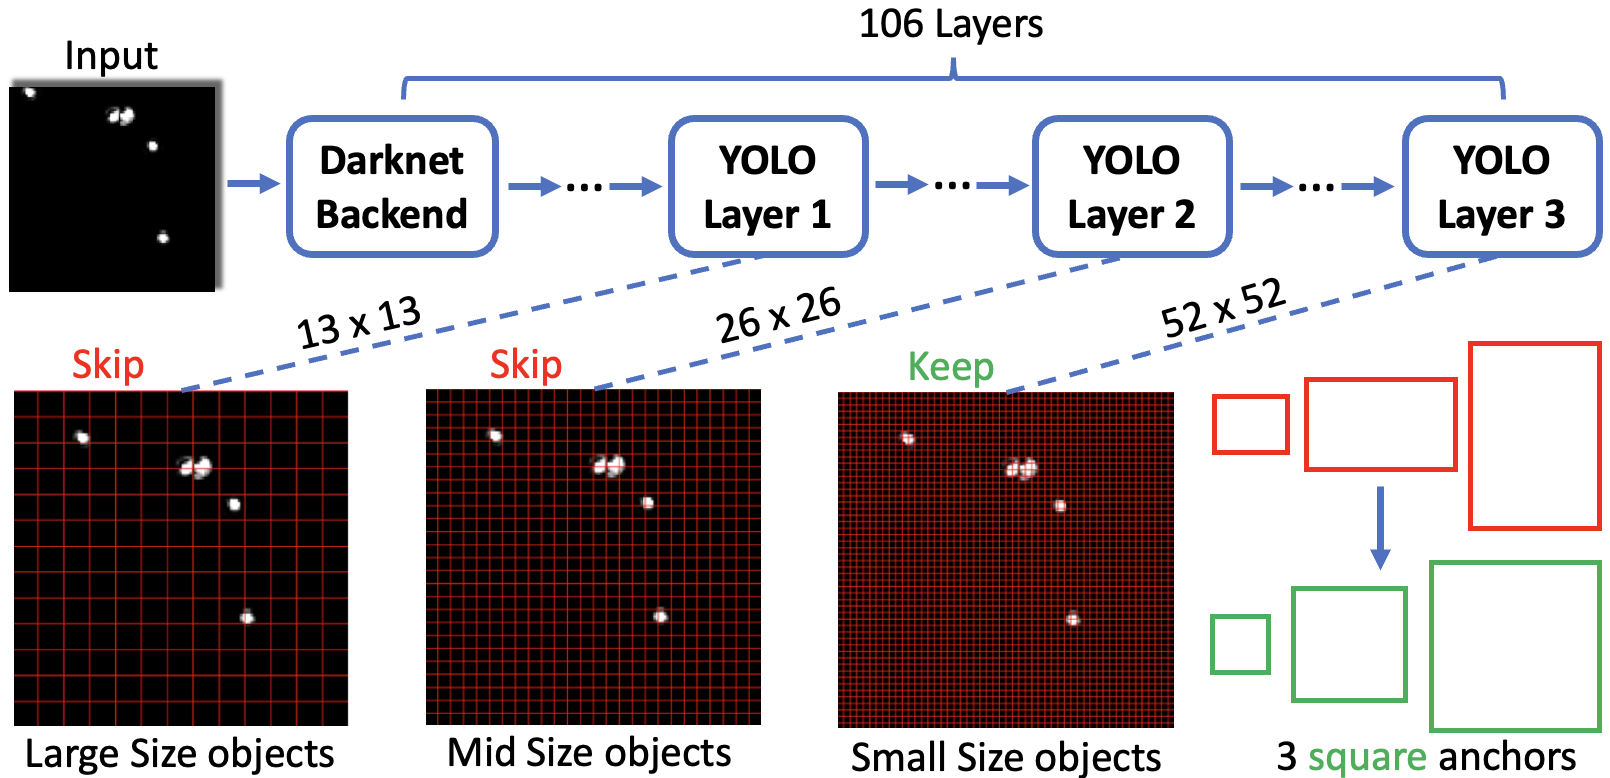
\includegraphics[width=0.75\textwidth]{chapters/wowmom-pmc/figures/yolo.png}
	\vspace{-0.1in}
	\caption{Our \yolocust in the second step of the \our. The two major customization are: (i) Use only the third YOLO layer that detects small size objects (the output of \yolocust is the bounding box predicted by the third YOLO layer and we use the center of the bounding box as the transmitter location), and (ii) change the rectangle anchors to square anchors.}
	\label{fig:yolo}
\end{figure}

\subsection{\bf Object-Detection Based Precise Localization: \yolocust} 

The simple hand-crafted method described in the previous subsection performs reasonable well in most cases in our simulations. 
However, its key drawback is that it needs appropriate threshold values that may vary from case to case; such thresholds can be difficult to determine, especially since
the input images (with distributions) are not expected to be perfect as they are themselves output of a learning model.
Inaccurate threshold values can lead to false alarms and misses. 
Also, the previous method is not sufficiently accurate at the sub-pixel level, where
each pixel may represent a large area such as $10m \times 10m$ or even $100m \times 100m$. Thus,
we propose a CNN-based learning method that overcomes the above shortcomings.  
CNN has been widely used for object detection in different areas~\cite{objectdetectionsurvey,alizadeh21}.

We frame this problem as an object detection task where the objective is to detect and localize
known objects in a given image. We observe that our second-step peak detection problem is essentially an object detection problem where the ``object" to detect is a ``peak".
Thus, we turn the \mtl problem of localizing multiple transmitters into detecting 
peaks in the images output by \imgimg model. 
For object/peak detection, we design \yolocust, our customized version of YOLOv3~\cite{yolov3}.
Fig.~\ref{fig:peaks} is a zoom-in of localizing two close by transmitters (peaks) in Fig.~\ref{fig:overall}(b).

\softpara{Peak Detection Using \yolocust.} 
Object detectors are usually comprised of two parts: (i) a backbone which is usually pre-trained on ImageNet, and (ii) a front part (head), which is used to predict bounding boxes of objects, probability of an object present, and the  object class. 
For the front part, object detectors are usually classified into two categories, i.e., one-stage detectors such as the YOLO~\cite{cvpr16-yolo} series, and two-stage detectors such as the R-CNN~\cite{cvpr14-rcnn} series.
We choose the one-stage YOLO series because of its computational efficiency, high popularity and available ways to customize it for our specific context. We refer to the customized version as \yolocust, see Fig.~\ref{fig:yolo}.
%%%%%%%%%
Implementing a 106-layer deep neural network with a complex design from scratch is
out of scope of our work. 
Thus, we use a publicly available source repository~\cite{yolo-github} and made customization on top of it.
We refer to the architecture that uses \imgimg $\ $and \yolocust in sequence as \our, our key product.  
In addition, we use \imgimg in combination with the uncustomized original YOLOv3,
and refer to it as \ouryolo (still change the class number to one).
%\blue{For the two important hyper-parameters of YOLOv3, object confidence threshold and intersect-of-union threshold for non-maximum suppression, we tweaked to 0.8 and 0.5 respectively.}

\softpara{Customization of YOLOv3}.
Overall, we incorporated four customization to YOLOv3, of which two are significant and the
other two are relatively minor. See Table~\ref{table:yolocust}. YOLOv3 is designed to be a general object detector that can detect objects of various sizes, shapes, and classes within input images
of various sizes. However, in our context, the input images are of a fixed size, with
only a single class of objects which are relatively small and semi-circular. 
Based on the above observations, we make changes to the original YOLOv3 that both 
decrease the model complexity and improve its performance.

\begin{figure}[t]
	\centering
	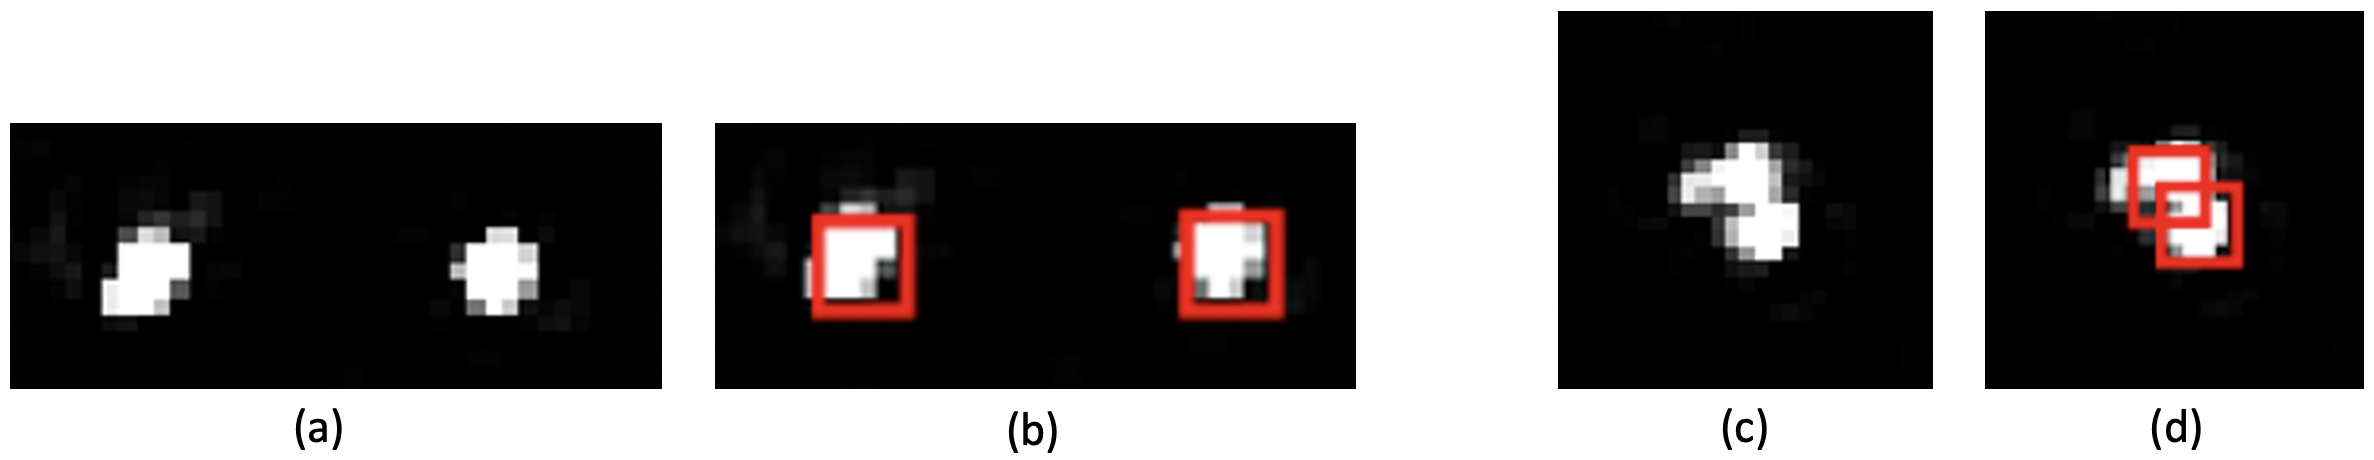
\includegraphics[width=0.75\textwidth]{chapters/wowmom-pmc/figures/peaks.png}
	\vspace{-0.1in}
	\caption{(a) is the zoom-in of two peaks at the bottom of the Fig.~\ref{fig:overall} example.
	(c) is the zoom-in of the two close by peaks in the middle right of the Fig.~\ref{fig:overall} example. (b) and (d) shows the bounding boxes that \yolocust outputs for (a) and (c) respectively.}
	\label{fig:peaks}
\end{figure}

\begin{table}[t]
    \caption{Differences between the original YOLOv3 and our \yolocust.}
    \centering
    \begin{tabular}{ |p{6cm}|p{6cm}| } 
     \hline
     YOLOv3 & \yolocust  \\
     \hline \hline
     Has three YOLO layers at $13\times13$, $26\times26$, and $52\times52$ for detection & Only use the last $52\times52$ YOLO layer for detection (skip the first two YOLO layers) \\
     \hline
     Has 3 different rectangle anchors for each YOLO layer & Has 3 square anchors \\
     \hline
     Every 10 batches, randomly chooses a new input image dimension size & Do not randomly choose new input dimension size \\ 
     \hline
     Has 80 different categories of object class & Only has one category for the peak class \\ 
     \hline
    \end{tabular}
    \label{table:yolocust}
\end{table}

{\em Customization Details}. 
The first and second changes presented in Table~\ref{table:yolocust} are major changes and we elaborate them in the following paragraphs.
%%%%%%%%o
Making prediction at three different scales is one of the highlights of YOLOv3 and an improvement comparing to the previous version YOLOv2 which was prone to missing at detecting small objects. 
As shown in Fig.~\ref{fig:yolo}, the coarse-grain $13\times13$ YOLO layer-1 is designed for detecting large size objects, 
the $26\times 26$ YOLO layer-2 is designed for detecting middle-sized objects, and 
the fine-grained $52\times52$ YOLO layer-3 is designed for detecting small-sized objects.
Since the peaks in our translated images are always small objects, we only use the last $52\times 52$ YOLO 
detection layer (and skip the first two YOLO layers).
%%%%%%%
As shown in Fig.~\ref{fig:yolo}, by ``skipping" the two YOLO layers means that we do not use them in 
computing the overall loss function and their outputs are not used in predicting the bounding boxes.
%\red{``Skip'' shown in Fig.~\ref{fig:yolo} is implemented as the first two YOLO layers are not calculated in the overall loss function and their outputs are not used for predicting bounding boxes.}
% Thus, the loss function depends only on the last 52x52 YOLO layer-3, instead of all three YOLO layers and the optimization process targets only the  the last 52x52 YOLO layer.
% \red{The above results in less parameter values to be learnt via training, and thus, reduces the training cost 
% substantially. }
%%%%%%%%%%%%%%%%%%
In our \yolocust, the only YOLO layer predicts 8112 bounding boxes, since it has a 
dimension of $52\times 52$ and each cell results in prediction of 3 bounding boxes; this is in contrast
to the original YOLOv3, which predicts 10647 bounding boxes ($3 \times (13\times13 + 26\times26 + 52\times52) = 10647$).

The anchor box is one of the most important hyperparameters of YOLOv3 that can be tuned to improve
its performance on a given dataset.  The original YOLO's anchor boxes are $10\times13$,  $16\times30$, and $33\times23$ (for
the input image of size $416\times416$ pixels), which are essentially bounding boxes of a rectangular shape. 
%%%%%%%%%%%%%
These original YOLOv3 anchors were designed for the Microsoft COCO \cite{mscoco} data set, and were chosen
since they best describe the dimensions of the real world objects in the MS COCO data set. In our context,
since the peaks are generally squares---we use the anchor boxes to be $15\times15$, $25\times25$, and $35\times35$.

%%%%%%%%%%% peaks %%%%%%%%%

\softpara{Input Image for \yolocust.}
The first step \imgimg's output image is $100\times100$, while the second step \yolocust's input is required\footnote{YOLOv3 was developed before our work and the YOLOv3 authors set the input size of the CNN model to $3\times416\times416$.~Although we are customizing their YOLOv3 model, we cannot change the input size because changing it will change the convolutional layer structure, which will 
preclude us from using the pre-trained weights in the YOLOv3 backbone.} 
to be a three-channel (RGB) image with each channel being size of $416\times 416$. 
%%%%%%%%%%%
To feed the output of \imgimg to \yolocust, we do the following: (i) First, we duplicate 
the \imgimg's output image to create two more copies and thus create a three-channel image
of 100 $\times$ 100 size channels; (ii) Next, we resize the $100\times100$ channels to $416\times416$ channels using the PyTorch's default ``nearest neighbor" interpolation. See Fig.~\ref{fig:yolo-preprocess}.

\softpara{Output of \yolocust.}
YOLO treats objected detection as a regression problem. The regression target (or ``label") for an object is a five-value tuple $(x, y,$ $length,$ $width, class)$. 
In our case, there is only one $class$. 
$x$ and $y$ are real number location coordinates of the center of the bounding box, which we use as the location of the transmitter. 
$Width$ and $height$ determine the size and shape of the object---which we consistently set to be 5 each to signify a $5\times5$ square. 
Note that the center of the bounding box is in the continuous domain. 
Thus, we are able to get sub-pixel level location of the transmitters.


\begin{figure}[t]
	\centering
	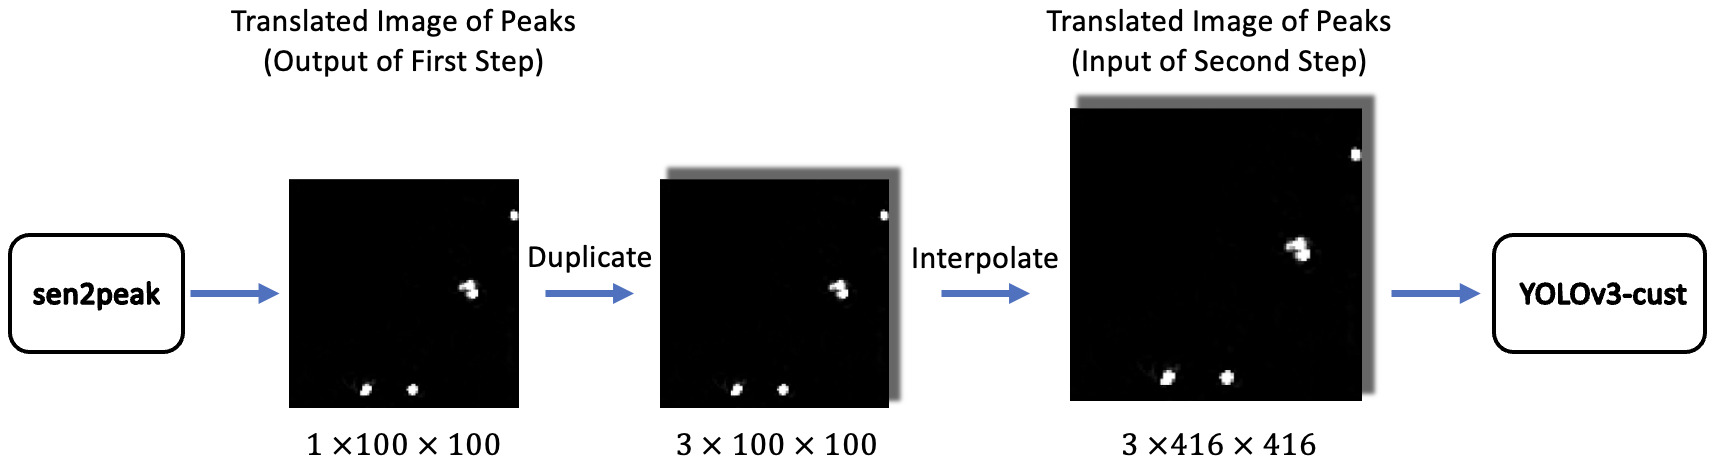
\includegraphics[width=0.9\textwidth]{chapters/wowmom-pmc/figures/yolo-preprocess.png}
	\vspace{-0.1in}
	\caption{The data processing of \imgimg's output to get \yolocust's input of correct size.}
	\label{fig:yolo-preprocess}
\end{figure}


%\blue{Labeling the training dataset of \yolocust is important. Given the output of the first step's \imgimg and the ground truth of the TX locations, we label the Gaussian peaks as a class peak who has a value higher than 0.3 at the ground truth's pixel location (recall in \ref{subsec:imgimg_output_image} that the peak at the target representation of a TX in \imgimg is 10). That is to say, when \imgimg outputs a very low altitude Gaussian distribution (i.e. near flat) for a transmitter, that near flat area will not be labeled as a peak for the training data of \yolocust.}


%In summary, we customized both the number of YOLO layers and anchor box configurations, to decrease the model complexity and increase accuracy for our context. The increase of accuracy of our system is demonstrated in the next section.

\section{Localization in the Presence of Authorized Users}
\label{sec:authorized}

Till now, we have assumed that the only transmitters present in the area are the intruders which need to be localized. In this section, we solve the more general \mtl problem, where there may be a set of authorized users in the background. 
This is referred to as the multiple transmitter localization - shared spectrum (\mtlss) problem \cite{ipsn20-mtl}.

In particular, in a shared spectrum paradigm, there are primary users and an evolving set of active secondary users transmitting in the background.
Different than the intruders whose locations are unknown, the authorized users' locations are known and we wish to utilize this known information to better localize the unknown intruders.
The key challenges come from the fact that the set of authorized users is not static and changes over time as allocation requests are granted and/or active secondary users become inactive over time.
A straightforward way to handle background authorized users is to localize every transmitter, and then remove the authorized users. 
However, any localization approach is susceptible to performance degradation with the increase in the number of transmitters to be localized.
Thus, the straightforward approach of localizing every transmitter is likely to be error-prone.
Therefore, we attempt to develop a new approach that uses \our as a building block that uses the information of the location of the authorized uses in a way other than removing them after localizing all.
The new approach tries to subtract the received signal strength at the sensors by a value received from the authorized users.
This subtraction is done by a novel CNN model; we refer to it as \subtract.
Then we feed the image with subtracted powers to the \our and get the locations of the intruders.
See Fig.~\ref{fig:subtractnet}(c)--(d)--(f).
We describe \subtract in the following paragraphs.

% \begin{figure}
%     \centering
%     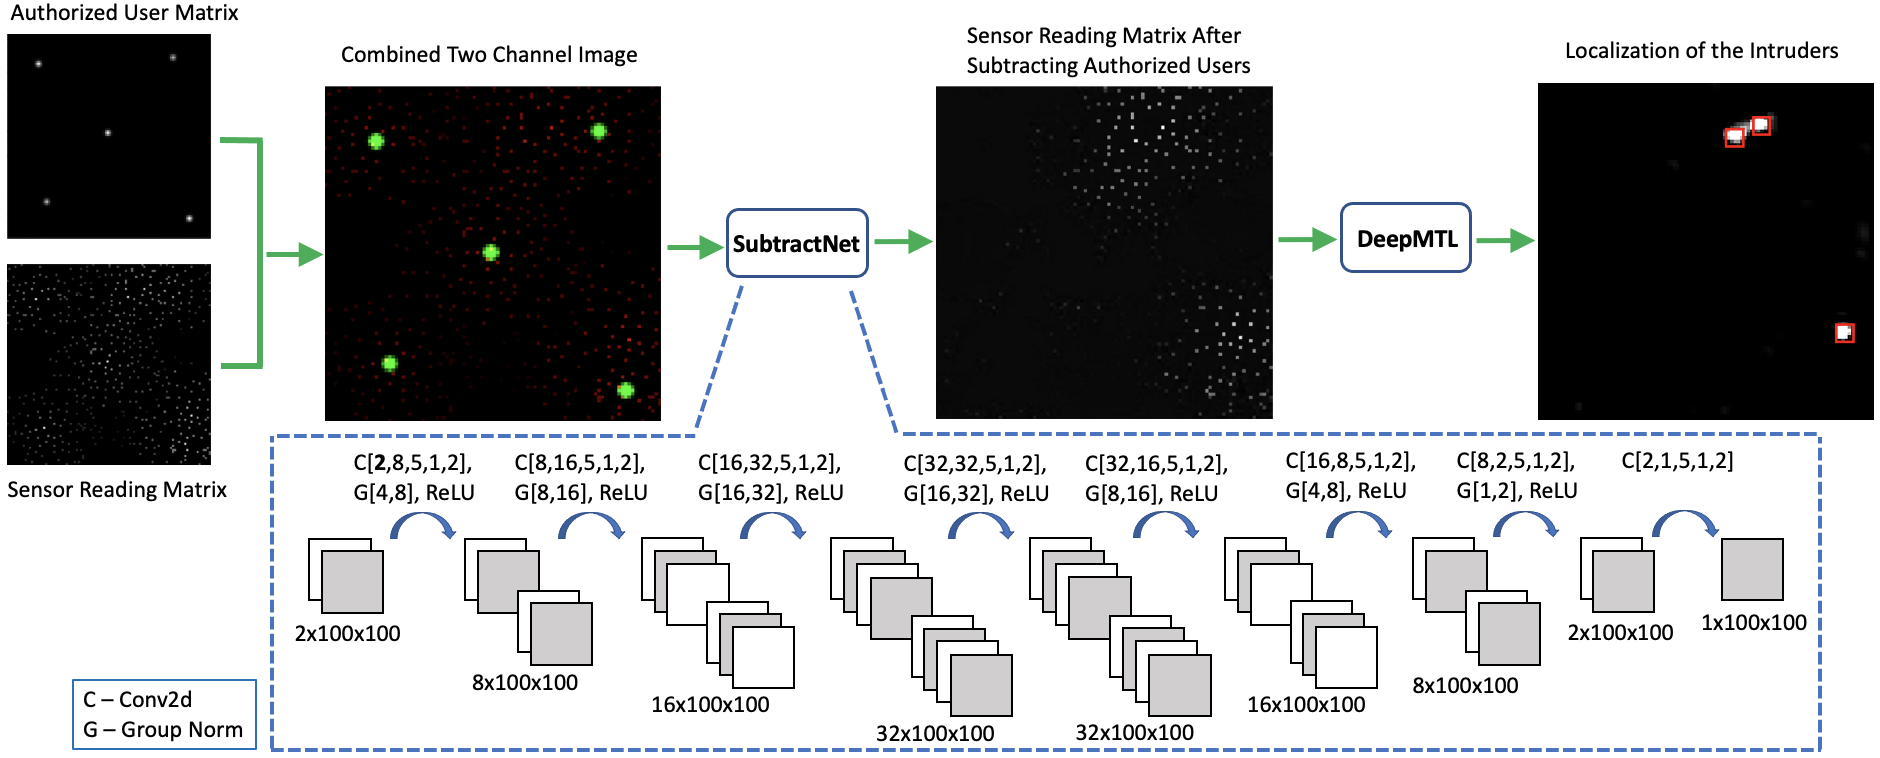
\includegraphics[width=\textwidth]{figures/subtractnet.png}
%     \vspace{-0.1in}
%     \caption{Overall architecture of second approach to localize 3 intruders in the presence of 5 authorized users (in color green). The details of the \subtract model is in the dotted box.}
%     \label{fig:subtractnet}
% \end{figure}

\begin{figure}
    \centering
    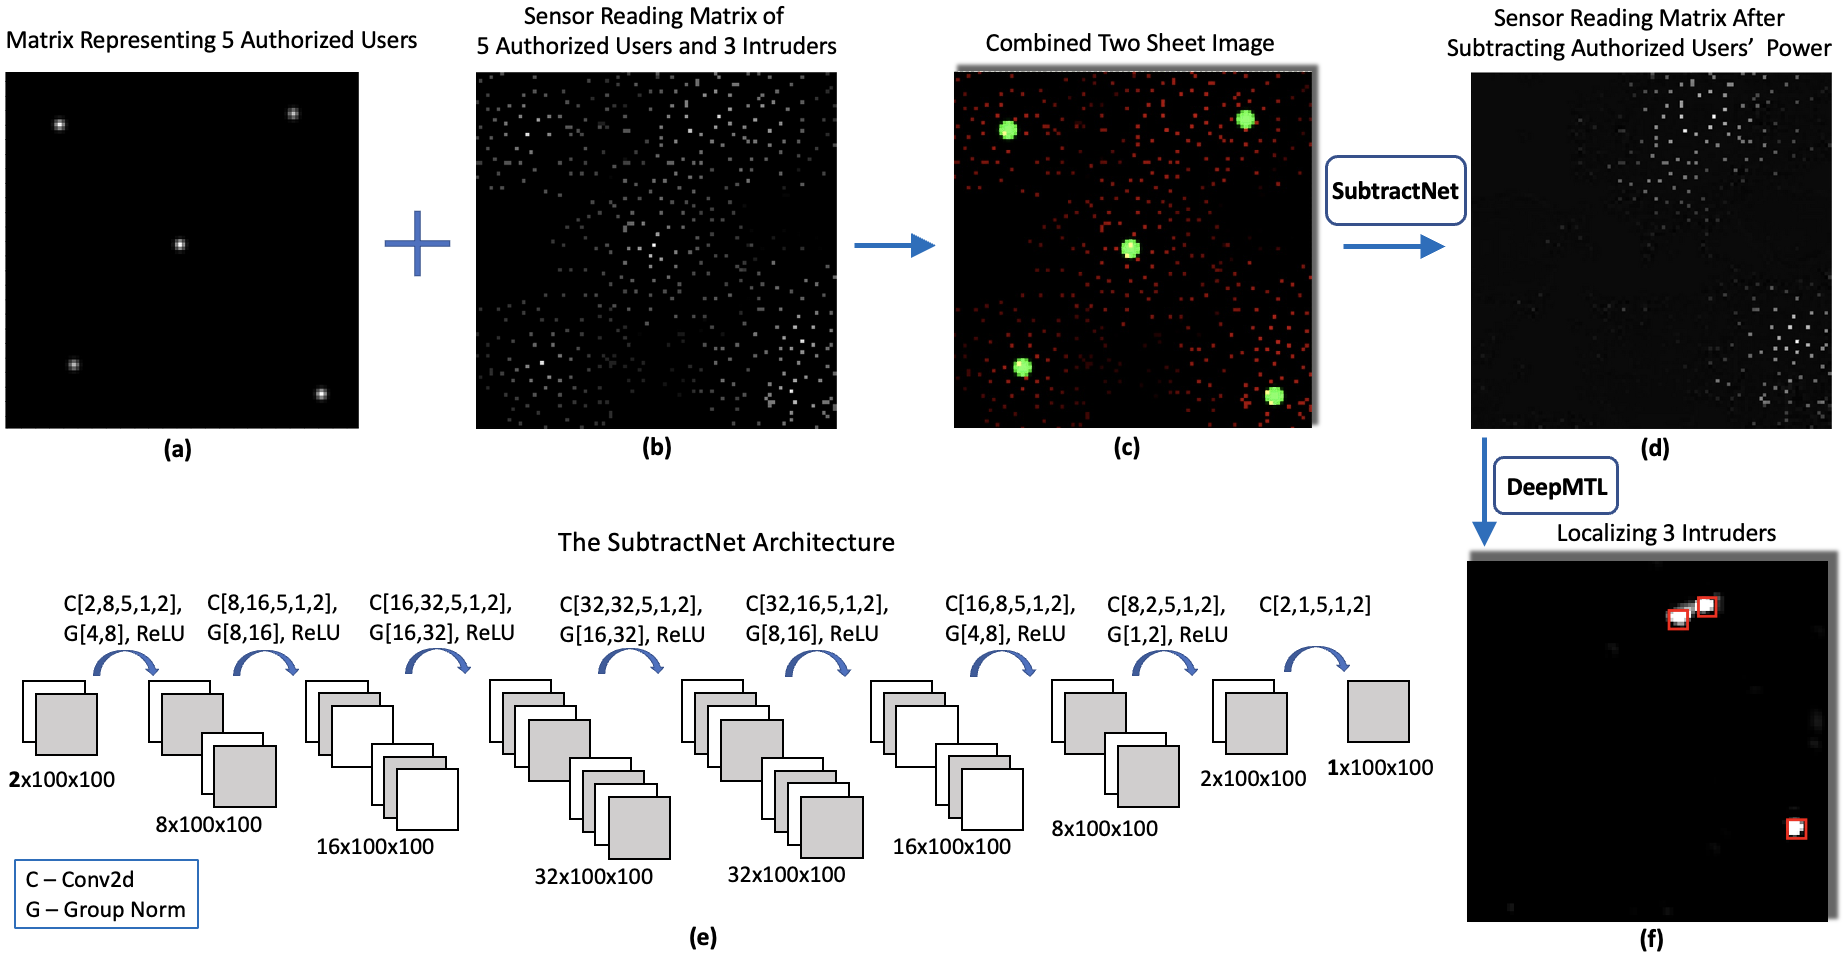
\includegraphics[width=\textwidth]{chapters/wowmom-pmc/figures/subtractnet2.png}
    \caption{Overall architecture of second approach to localize 3 intruders in the presence of 5 authorized users. The input of the \subtract is (c), which is stacking authorized user matrix (a) and the sensor reading matrix (b). (d) is the output of \subtract, where the transmission power of the authorized users is subtracted from the area. The details of the \subtract model is in (e). (f) is the localization output after feeding (d) into \our.}
    \label{fig:subtractnet}
\end{figure}

\softpara{\subtract Input Image}. The sensor reading has two sources, one is the intruders and the other is the authorized users.
We aim to subtract the power of the authorized users and remain the power from the intruders.
So the input of the \subtract will contain two kinds of information: the authorized users' information (Fig.~\ref{fig:subtractnet}(a)), including both the location and the transmitter power, and the sensor reading matrix (Fig.~\ref{fig:subtractnet}(b)) that encode the power from all transmitters.
To incorporate the two kinds of information, we first encode the authorized user information into a matrix that has the same dimension as the sensor reading matrix.
Then stack the two matrices together.
The combined stacked image is nothing but a two-channel image, which can be interpreted as Red and Green channels.
The sensor reading matrix is the Red channel and the authorized user matrix is the Green channel. There is no Blue channel.
To represent the authorized transmitter in the Green channel, we use a Gaussian peak similar to what we did in the \imgimg for representing transmitters (Section \ref{sec:translate}).
The difference is that in \imgimg, all the peaks have a uniform height, whereas in \subtract, the height of the peak is the power of the authorized transmitter.
So the higher the power of the authorized transmitter, the higher the peak in the Green channel.
Another difference is that the authorized transmitters are approximated at discrete locations instead of the continuous locations as in \imgimg.

\softpara{\subtract Output Image}. 
The \subtract's output image is just a one-channel images and represents the sensor readings due to the intruders only.  

\softpara{\subtract CNN Architecture}.
We refer to the model that subtracts the power from the authorized users as the \subtract. 
It has a similar design philosophy with \imgimg.
\subtract is also an image-to-image translation neural network.
Compared to \imgimg, it doubled the number of layers, mainly because \subtract needs a bigger receptive field than \imgimg.
A bigger receptive field can let the CNN model update sensors that are further away from the authorized user.
For the loss function, we use the L2 loss function, similar to the loss function used in Equation~\ref{equ:sen2peak_loss}, merely replacing the \imgimg with \subtract in Equation~\ref{equ:sen2peak_loss}.
The training details are also the same as in \imgimg.

\section{Estimating the Transmit Power of Transmitters}
\label{sec:power}

In this section, we extend our techniques to estimate the transmit power of the
intruders; we refer to the overall problem as  Multiple Transmitter Power Estimation (\mtpe). Estimation of the transmit power of transmitters can be very useful in the shared
spectrum systems. In particular, estimated transmit powers of the primary users (if unknown, as in the case of military users or legacy systems) can be used to set a
``protective" region around them---inside which secondary users can be disallowed~\cite{Ureten2011powerlocation}.
%%%%%%%
Estimating transmit power of secondary users can also be useful. E.g., if the violation
in a shared spectrum system is based on a certain minimum threshold, then it is important to estimate the transmit power to determine a violation. 
Also, the estimated transmit power of secondary users can also be used to ``circumvent" their intrusion---i.e., for the primary users to appropriately increase their transmit power to overcome the harmful interference from the secondary users. 
%%%%%%%%
In general, estimating the transmission power is beneficial to various operations such as node localization, event classification, jammer detection \cite{PowerEstimate2010Zafer}.
 
There are several works that estimates the transmission power of a single transmitter, often jointly with its location \cite{PowerEstimate2010Zafer, Ureten2011powerlocation, icoin2007-powerposition}.
Our previous work \cite{ipsn20-mtl} can estimate the power of multiple transmitters.
The similarity among all four of these methods is that they are estimating the power and location jointly.
In this paper, we propose a new method that leverages the capabilities of \our by using it as a building block. We first localize the transmitters by \our. 
Then given the localized locations, estimate the transmitters' transmission power by a newly designed CNN model \power. 
Although \power is designed to only estimate the power of a single transmitter, we use it together with a machine learning-based error correction method that can mitigate the errors while applying \power to the multiple transmitter power estimation scenario.

In this section, we develop a technique to predict the transmission powers of the intruders. Here, for simplicity, we assume no background authorized users, though, the techniques in this section also work in the presence of authorized users. 
%%%%%%
We leverage our accurate and robust localization solver that tolerates varying transmission power for different transmitters (the varying transmission power needs to be in a range).
We propose an efficient approach and its overall methodology at a high-level is as follows.
And then in the next subsection we describe our \power model.
%%%%%%%%
\begin{enumerate}
\item We use \our to localize the multiple transmitters in a field. 
\item We develop a CNN model \power to predict power of a single isolated (far away from other intruders) intruder. 
\item For other (non-isolated) intruders, we still use \power to predict their powers but employ a post-processing ``correction" technique to account for nearby intruders. 
\end{enumerate}
%%%%%%%%%%%%%%%%%%%


\subsection{\bf \power: Predicting Power of a Single Isolated TX}
\label{subsec:in-out-design}

\softpara{\power Input Image}. 
Let us consider an ``isolated" transmitter $T$. 
To predict $T$'s power, we start with
creating a smaller-size image by cropping the original sensor readings image with the area of a certain size around $T$. 
%%%%%%
In our evaluations in Section \ref{sec:evaluation}, the transmitters have a transmit radius\footnote{I.e., sensors beyond a distance of 20 pixels away from a transmitter $x$ receive only negligible power from $x$.}
of around 20 pixels, which is equivalent to 200 meters.\footnote{Transmission ranges of a standard 2.4 GHz and 5 GHz WiFi at default transmission powers (100 mW) are roughly 45m and 15m respectively. 
In our simulations (Section \ref{sec:evaluation}), we use the 600 MHz frequency band. 
As the lower the signal frequency, the higher the transmission range, a transmission range of around 200m is reasonable.}
For this setting, we used an cropped area of $21 \times 21$ around the isolated transmitter $T$ to predict its power, with $T$ is at the center of this area; also, in this setting, we define a transmitter to be {\em isolated} if there is no other transmitter within a 20-pixel 
distance.\footnote{Ideally, transmitters with a transmit radius of 20 pixels should entail defining isolated transmitters as ones that have no other transmitters within a 40-pixel distance, and then use a
$41\times41$ area around the isolated transmitter. However, in our evaluations, our chosen values yielded a more efficient technique with sufficient accuracy.}
%%%%%%%% 
%%%%%%%%%%%%%%%%%
% We choose a $21 \times 21$ cropped size \blue{because this size is large enough to cover {\em most} surrounding sensors that receive power from the transmitter. 
% %%%%%%%%%%%%
% A larger cropped size, such as $41 \times 41$ grid, will contain {\em all} surrounding sensors that receive power from the transmitter, but will also likely contain some sensors at the edge of this cropped grid who will receive more power from the other transmitters in the case where the transmitters are not ideally isolated (which will happen in reality).}
% So cropping the input to a smaller size will decrease the complexity of the neural network model, thus making the model easier to train.
Note that the above cropping process requires the location of the transmitter to be known, and hence, we undertake the above power-estimation process after the localization of the transmitters using the \our model.  
%%%%%%%%%%%%%%%%%%%%%%%%%%%
We crop images from the same dataset where \our is trained on.

\softpara{\power Output Power}.
The output of the \power is a single pixel whose value is the predicted power of the transmitter located at the center of the cropped image.
Before coming into this single pixel output design, we tried using the height or radius of the peak from the output of \imgimg to indicate the power. 
But we figure out that the height or radius of the peak is hard to accurately predict and therefore is not an accurate indicator of the power.
\eat{We also tried to borrow the density map idea from the crowd counting literature~\cite{ECCV18-crowdcount,aaai21-topocrowdcount} from the computer vision community.
In crowd counting solutions, the CNN model predicts a density map and the summation of the value of all the pixels is the number of crowd, i.e., the number of persons in an image.
We tried to create a concept called power density map so that the summation of the pixel values equals to the power of a transmitter.
But it didn't work out well either.
In the end, we figured out that directly predicting a floating point scalar value is the right way.
The other ways are just doing thing indirectly and making the CNN model more complex and harder to train.}
So we reduced the output complexity and designed the output as a simple single pixel whose value directly represents the power of the transmitter.
By simplifying both the input side and output side, we can design and implement a novel CNN model that can accurately predict the power of a single transmitter, as described in the following paragraph.

\begin{figure}
    \centering
    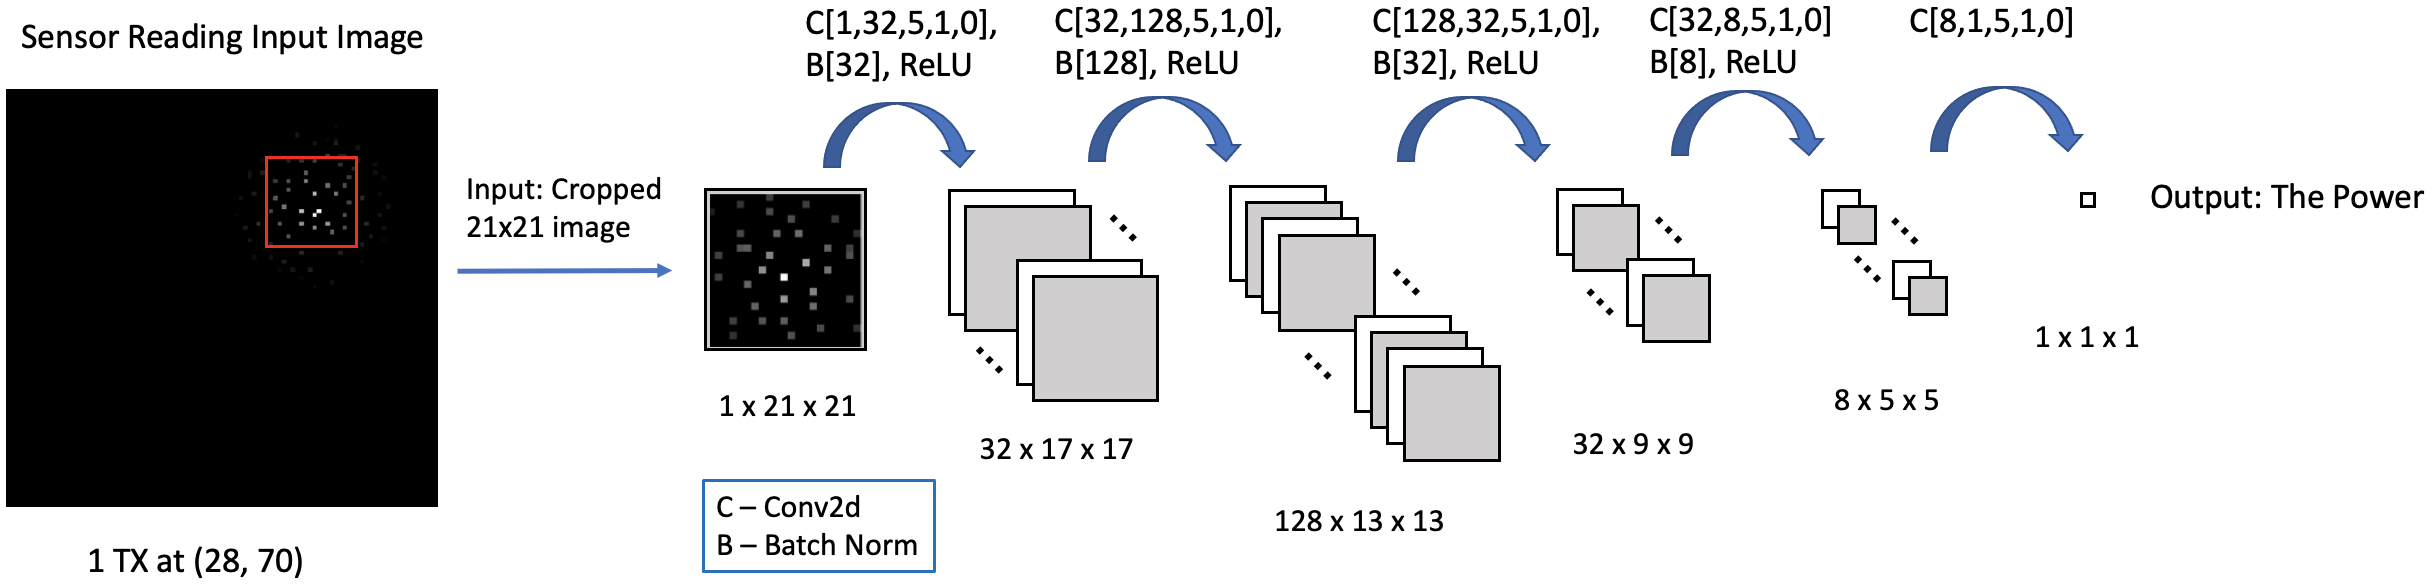
\includegraphics[width=\textwidth]{chapters/wowmom-pmc/figures/power_predictor.png}
    \caption{Architecture of the \power, a five-layer CNN model that takes in a cropped image from the original input image and outputs the predicted power of one transmitter. The figure displays how the data volume flows through the various convolutional layers. C stands for Conv2d, a 2D convolutional layer, and for each Conv2d layer, the five values shown are [number of input channel, number of output channel, kernel size, stride, padding]. B stands for batch normalization 2d, and for each batch normalization, the value shown is [number-of-features].}
    \label{fig:power_predict}
\end{figure}


\softpara{\power CNN Architecture.}
We refer to our CNN model that estimates the power of a single transmitter as \power.
See Fig.~\ref{fig:power_predict}.
It has a similar design to \imgimg as well, where it has no max-pooling layers and no fully connected layers.
We do not use the fully connected layers and design a fully-convolutional network since the usage of fully connected layers will destroy the spatial relationships.
\power has five CNN layers and each CNN layer has a kernel size $5\times5$, striding 1 and padding 0.
With this setting, a pixel in the output layer has a receptive field of $21\times 21$, which is exactly the size of the input cropped image. Also note that the pixel is exactly at the location where the transmitter is assumed to be located (recall that the transmitter is at the center of the cropped image).
We tried both batch normalization and group normalization and found that batch normalization is better than group normalization, which is the opposite to the \imgimg scenario.
ReLU is used as the activation function.
% So each pixel at the output layer can ``see" the entire input image.

{\em Loss Function.} The output of the last convolutional layer is technically a 3D cube, although $1 \times 1 \times 1$. So we flatten it in the end to get one scalar value.
We use a L2 loss function, which is formally defined as:
\begin{equation}
 \frac{1}{N} \sum_{i}^{N} (\power(X^c_{i}) - y_i)^2,
\end{equation}
where $N$ is the number of training samples,~$X^c_{i}$ is the cropped input image for the $i^{th}$ sample and $y_i$ is the ground truth power for the $i^{th}$ sample.
$\power(X^c_{i})$ is the predicted power.
We use Adam as the optimizer, and set the learning rate to 0.001 and the number of epochs to 20, which is sufficient for the model convergence.

\subsection{ \bf Estimating Powers of Multiple Transmitters}
Our end goal is to estimate the power of multiple transmitters at the same time. 
When the multiple transmitters are far away and isolated from each other, the problem reduces to single transmitter power estimation, which \power handles well.
The hard part is to estimate transmit powers of multiple transmitters that are close by. 
In this case, a sensor will receive an aggregated power from multiple transmitters. We assume that blind source power separation is not viable. 

\subpara{Overall High-Level Approach}.
For each localized intruder by using \our (whether isolated or not), we crop the $21\times 21$ size area around it and feed it to \power, and estimate its power. If it is actually isolated, then the predicted power is final. If it is not isolated, then we apply a post-processing correction phase to account for the overestimation of the powers, as described below.

\eat{
One idea is to design a CNN model that can directly predicts the power of multiple transmitters.
But this is non-trivial.
Actually, it is the fact that we are having a difficult time directly predicting multiple transmitter power that lead us design \power that only predicts the power a single transmitter.
A core reason is that it requires more complex input and output to predict the power of multiple transmitters, and it is by largely reducing the input and output complexity that we are able to achieve single transmitter power estimation.}

\eat{but To explain the hardness, let's go back to the design choice of \power.
The two key design of \power are that 1) the location of the single transmitter whose power is being estimated is right at the center of the cropped input image and 2) the output of the model is only one pixel whose value is the estimated power of that single transmitter.
However, when a CNN model wishes to directly estimate the power of multiple close by transmitters, two issues arrives:
1) Where to crop the image? You either crop the image centered at one arbitrary transmitter or at the geo-center of multiple close by transmitters.
Or you don't crop at all and take in the whole sensor readings input image, which only increase  the complexity and make the model more difficult to train.
2) The output cannot be a single pixel and must be multiple pixels to represent multiple transmitters.
But the number of close by transmitters is unknown.
So it need multiple models that has a different number of output pixels in the last layer and then do a matching that match a pixel to a specific transmitter.
Image translation based methods introduced in section~\ref{sec:translate} can avoid having multiple models, but it doesn't work well even for the single power estimation.
Given all the difficulties above, we come up with an approach that avoids them and workaround.}

\softpara{Correction Method for Close by Transmitters}.
Let us first consider the case where there are two close by transmitters $T_0$ and $T_1$. We use \power to estimate the power of two transmitters and get $p_0^{'}$ and $p_1^{'}$ respectively.
Let us say the ground truth are $p_0$ and $p_1$ respectively.
The estimated power will most likely be higher than the ground true power, i.e., $p_0^{'} > p_0$ and $p_1^{'} > p_1$.
Because \power can only ``see" one transmitter, and it will view two transmitters in the areas as a combined single one.
Let us focus on $T_0$  and assume $\delta_0 = p_0^{'} - p_0$.
The intuition is that $\delta_0$ has some underlying patterns that we are able to recognize.
We model $\delta_0$ as a function of some features related to $T_0$ and $T_1$.
We model $\delta_0$ as follows,
\begin{equation}
  \delta_0 =   \theta_0 \cdot p_0^{'} + \theta_{(1,1)} \cdot d_{01} + \theta_{(1,2)} \cdot p_1^{'} + \theta_{(1,3)} \cdot \frac{p_1^{'}}{d_{01}} 
  \label{equ:twotxpower}
\end{equation}
where $d_{01}$ is the distance between $T_0$ and $T_1$, and the four $\theta$s are the coefficients for the four terms respectively.
The first term is related to $T_0$ itself, and the other three terms are related to $T_1$.
We observe that the smaller the $d_{01}$, the larger the value of $\delta_0$.
And the bigger the $p_{1}^{'}$, the larger the value of $\delta_0$.
So $d_{01}$ has a negative correlation with $\delta_0$ while $p_{1}^{'}$ has a positive correlation.
$\frac{p_1^{'}}{d_{01}}$ is a combination of two terms to increase the number of features.
We also tried a few other features, but we decided to use only these three features for a close by transmitter as a balance of model accuracy and model complexity.

Equation~\ref{equ:twotxpower} is for the case of one close by transmitter, we then extend the equation to handle multiple close by transmitters in the following Equation~\ref{equ:multitxpower},
\begin{equation}
  \delta_0 =  \theta_0 \cdot p_0^{'} + \sum_{i=1}^{m} ( \theta_{(i,1)} \cdot d_{0i} + \theta_{(i,2)} \cdot p_i^{'} + \theta_{(i,3)} \cdot \frac{p_i^{'}}{d_{0i}})
  \label{equ:multitxpower}
\end{equation}
where $m$ is the number of close by transmitters for $T_0$, the transmitter of interest, $d_{0i}$ is the distance between $T_0$ and close by $T_i$, and $p_i^{'}$ is the uncorrected power predicted by \power. 
For the $i$th close by transmitter, we introduce three terms $ d_{0i},  p_i^{'}, \frac{p_i^{'}}{d_{0i}}$, and assign three coefficients $ \theta_{(i,1)}, \theta_{(i,2)}, \theta_{(i,3)}$ to the three terms respectively.
So for $m$ close by transmitters, there are $1 + 3m$ number of terms in the Equation~\ref{equ:multitxpower}.

After modeling $\delta_0$, in Equation~\ref{equ:correct}, we ``correct'' $p_0^{'}$ by subtracting $\delta_0$ from $p_0^{'}$ to get more an accurate estimation of the power of transmitter $T_0$.
\begin{equation}
    p_{0}^{correct} = p_{0}^{'} - \delta_0
    \label{equ:correct}
\end{equation}

\softpara{Estimating the parameter $\theta$}.
Equation~\ref{equ:multitxpower} is essentially a linear model and we can train it by using either linear, ridge, or LASSO regression models~\cite{scikit-learn}.
We perform experiments using ridge regression (alpha=0.01). 
We set a distance threshold for a neighbor transmitter to be classified as a close by transmitter. 
Note that the transmitters will have a different number of close by transmitters. 
So, let us denote $M$ as the maximum number of close by transmitters we see in the dataset.
When training the linear model in Equation~\ref{equ:multitxpower}, we train a model that assumes a maximum $M$ number of close by transmitters, i.e., the linear model has $1+3M$ terms.
The $3M$ terms are organized in a group of three (i.e., three features) and the groups are sorted by distance in an ascending order.
Then, for a transmitter with a smaller than $M$ number of close by transmitters, let us say $m$, only the first $1+3m$ terms will have a meaningful value.
And for the rest $3(M-m)$ terms, we set the value to zero, i.e., impute missing value with zero.
\section{Evaluation}
\label{sec:evaluation}

To evaluate the performance of our proposed techniques, we conduct large-scale simulations over
two settings based on two different propagation models. In particular, we consider the log-distance-based
propagation model and the Longley--Rice model obtained from SPLAT!~\cite{splat}. We evaluate various 
algorithms, using multiple performance metrics as described below. 

\para{Performance Metrics.} We use the following metrics 1, 2, and 3 to evaluate the localization methods and use the 4th metric to evaluate the power estimation methods.
\begin{enumerate}
    \item Localization Error ($\lerr$)
    \item Miss rate ($\mr$)
    \item False Alarm rate ($\fr$)
    \item Power Error ($\perr$)
\end{enumerate}
Given a multi-transmitter localization solution, we first compute the $\lerr$ as
the minimum-cost matching in the bi-partite graph over the
ground truth and the solution's locations, where the cost of each edge in the graph is the Euclidean distance between the matched ground truth node location and the solution's node location.
We use a simple greedy algorithm to compute the min-cost matching.
%%%%
The unmatched nodes are regarded as false alarms or misses. 
We also put an upper threshold on the cost ($\lerr$) of an eligible match. 
E.g., if there are four intruders in reality, but the algorithm predicts six
intruders then it is said to incur zero misses and two false alarms, so the $\mr$ is zero and the $\fr$ is one-third. 
If the algorithm predicts three intruders then it incurs one miss and zero false alarms, so the $\mr$ is one-fourth and the $\fr$ is zero.
In the plots, we stack the miss rate and false alarm rate to reflect the overall performance.


\para{Algorithms Compared.} 
We implement\footnote{Source code at: \url{https://github.com/caitaozhan/deeplearning-localization}.} and compare six algorithms in two stages. In stage one, we compare three versions of our
techniques, viz., \our, \ouryolo, and \ourpeak.  Recall that \our, \ouryolo, and \ourpeak 
use \imgimg in the first step, and \yolocust, original YOLOv3, and \simpeak respectively in the second step. In the first stage of our evaluations, we will show that 
\our outperforms \ouryolo and \ourpeak in almost all performance metrics. 
Thus, in the second stage, we only compare \our with
schemes from three prior works, viz., \splot~\cite{mobicom17-splot}, \deeptx~\cite{icccn20-deeptxfinder},
and \map~\cite{ipsn20-mtl} and show that \our outperforms the prior works.

\para{Training and Testing Dataset.}
We consider an area
%\footnote{To deal with areas of larger than 1 square kilometers, a tiling method similar to the one in \cite{icccn20-deeptxfinder} can be used. Tiling is not the focus of this work.} 
of $1km \times 1km$, and use grid cells (pixels) of 
$10 m \times 10 m$, so the grid is $100\times100$. 
The transmitters may be deployed
anywhere within a cell (i.e., their location is in the continuous
domain), while the sensors are deployed at the centers of the grid cells (i.e. their location is in the discrete domain).
%%%%%%%
For each instance (training or test sample), the said number of sensors and transmitters are deployed in the field randomly. 
For each of the two settings (propagation models described below), we create a 100,000 sample training dataset to train our models and create another 20,000 sample testing dataset to evaluate the trained model. 
%\red{Each dataset consists of samples with varying  number of transmitter, 
%varying sensor density, and varying transmitter power (0 to 5 dBm). 
%Even for the same sensor density, training  and testing samples may have sensors
%at different locations.}

We will evaluate the performance of various techniques for
varying number of transmitters/intruders and sensor
density. When we vary a specific parameter, the other parameter
is set to its \emph{default} value; the number of transmitters varies from 1 to 10 and the default value is 5; the sensor density varies from 1\% to 10\% and the default value is 6\% (600  sensors in a $100\times100$ grid).
The two default numbers 5 and 6\% are chosen because they are in the middle of their ranges.
When not mentioned, the default values are used.
The transmitter power varies from 0 to 5 dBm and is randomly picked.
To minimize overfitting, the training dataset and testing dataset have sensors placed at completely different locations.
%%%%%%%%%%%%%%%%%%%%%%%%%%%%%%%%%%%

We train the \our model using the 100,000 sample dataset. To train the \deeptx~\cite{icccn20-deeptxfinder}, we partition the 100,000 sample training dataset into ten datasets based on the number of transmitters in the samples which varies from 1 to 10. 
These ten datasets are used to train the ten ``localization" CNN models in \deeptx, and the full dataset of 100,000 samples is used to train the \deeptx model that determines the number of transmitters. 
%%%%%%%%%
For the \map scheme~\cite{ipsn20-mtl}, we assume the availability of all required probability distributions. We note that using a simple cost model (number of samples need to be gathered), 
the overall training cost for \map is an order of magnitude higher than \our and \deeptx. 
Lastly, \splot~\cite{mobicom17-splot} does not require any training.




%%%%%%%%%%%%%%

\para{Two Propagation Models and Settings}.
The sensor readings (i.e. the dataset) are simulated based on a propagation model. 
% Note that the propagation model is only used to simulate/generate samples, and the techniques developed themselves do not assume any propagation model. 
To demonstrate the generality of our techniques, we consider two propagation models as described below. 

\softpara{Log-Distance Propagation Model and Setting.}
Log-Distance propagation model is a generic model that extends Friis Free space model 
which is used to predict the path loss for a wide range of environments. 
As per this model, the path loss (in dB) between 
two points $x$ and $y$ at a distance $d$ is given by: $PL_d = 10\alpha\log{d} + \mathcal{X},$
where $\alpha$ (we use 3.5) is the path-loss exponent and $\mathcal{X}$ represents the shadowing effect that can be represented by a zero-mean Gaussian distribution with a certain (we use 1) standard deviation. 
Power received (in dBm) at point $y$ due to a transmitter at point $x$ with a 
transmit power of $P_x$ is thus: $P_{x} - PL_d$.
Power received at point $y$ due to multiple sources is assumed to be just an 
aggregate  of the powers (in linear) received from each of the sources.

% In this subsection, we evaluate our techniques on a data set generated from a more realistic propagation model, the Longley-Rice ~\cite{chamberlin82} Irregular Terrain With Obstruction Model (ITWOM). 
% We conduct one set of experiments based on this data set. We compare \our with \deeptx, \map, and \splot, and show \our is better.

\softpara{SPLAT! Model and Setting.}
This is a complex model of wireless propagation based on many parameters including locations, terrain data, obstructions, soil conditions, etc.
We use \splat~\cite{splat} to generate path-loss values. \splat is an open-source software implementing the Longley-Rice ~\cite{chamberlin82} Irregular Terrain With Obstruction Model (ITWOM) model.
%%%%%%%%%%%%%%%%%%%%
We consider a random area in Long Island, New York of $1km \times 1km$ large and use the 600 MHz band to generate path losses.
% As the height of an entity is an important factor in determining the
% path loss, we place the transmitters (PU or SU) at a height of 30m and the 
% receivers (PURs and SSs) at 15m above the ground level.


%%%%%%%% compare ours $$$$$$$$$$$$$

\begin{figure}[ht]
	\centering
	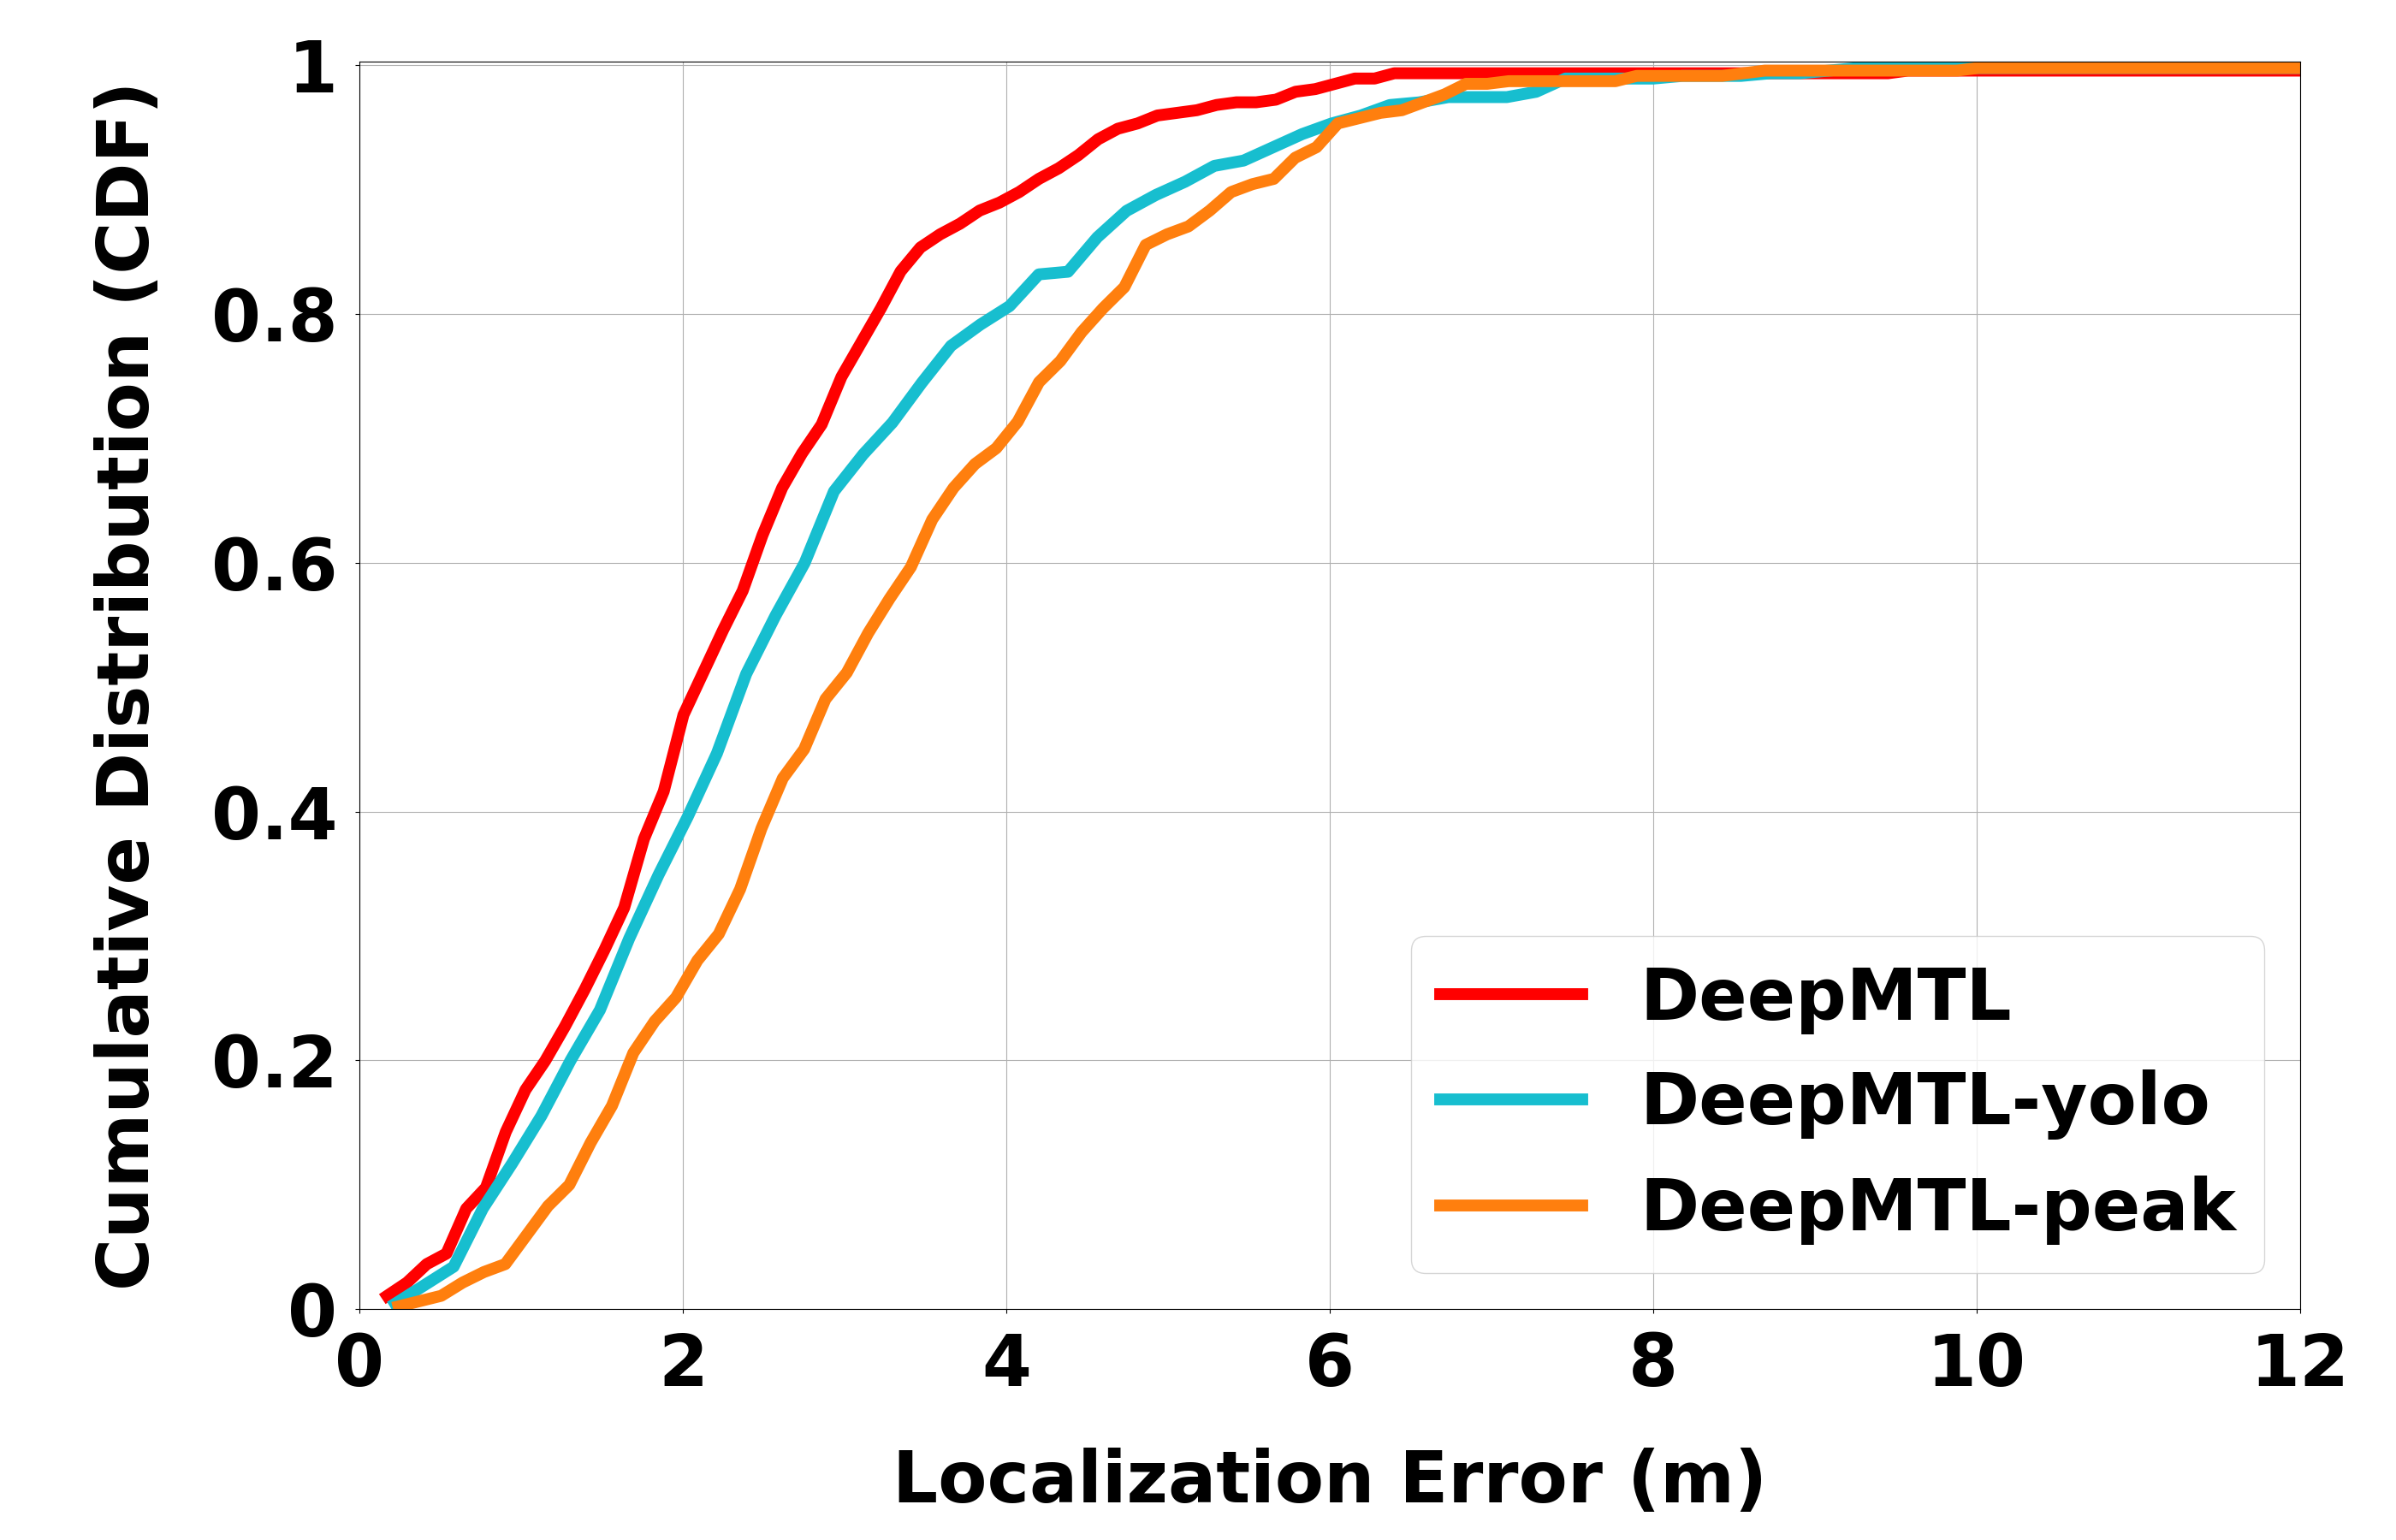
\includegraphics[width=0.6\textwidth]{chapters/wowmom-pmc/figures/ours_cdf.png}
	\caption{Cumulative probability of localization error of \our, \ouryolo and \ourpeak, for the special case of single transmitter localization with 6\% sensor density.}
	\label{fig:ours_cdf}
\end{figure}

\begin{figure}[ht]
	\centering
	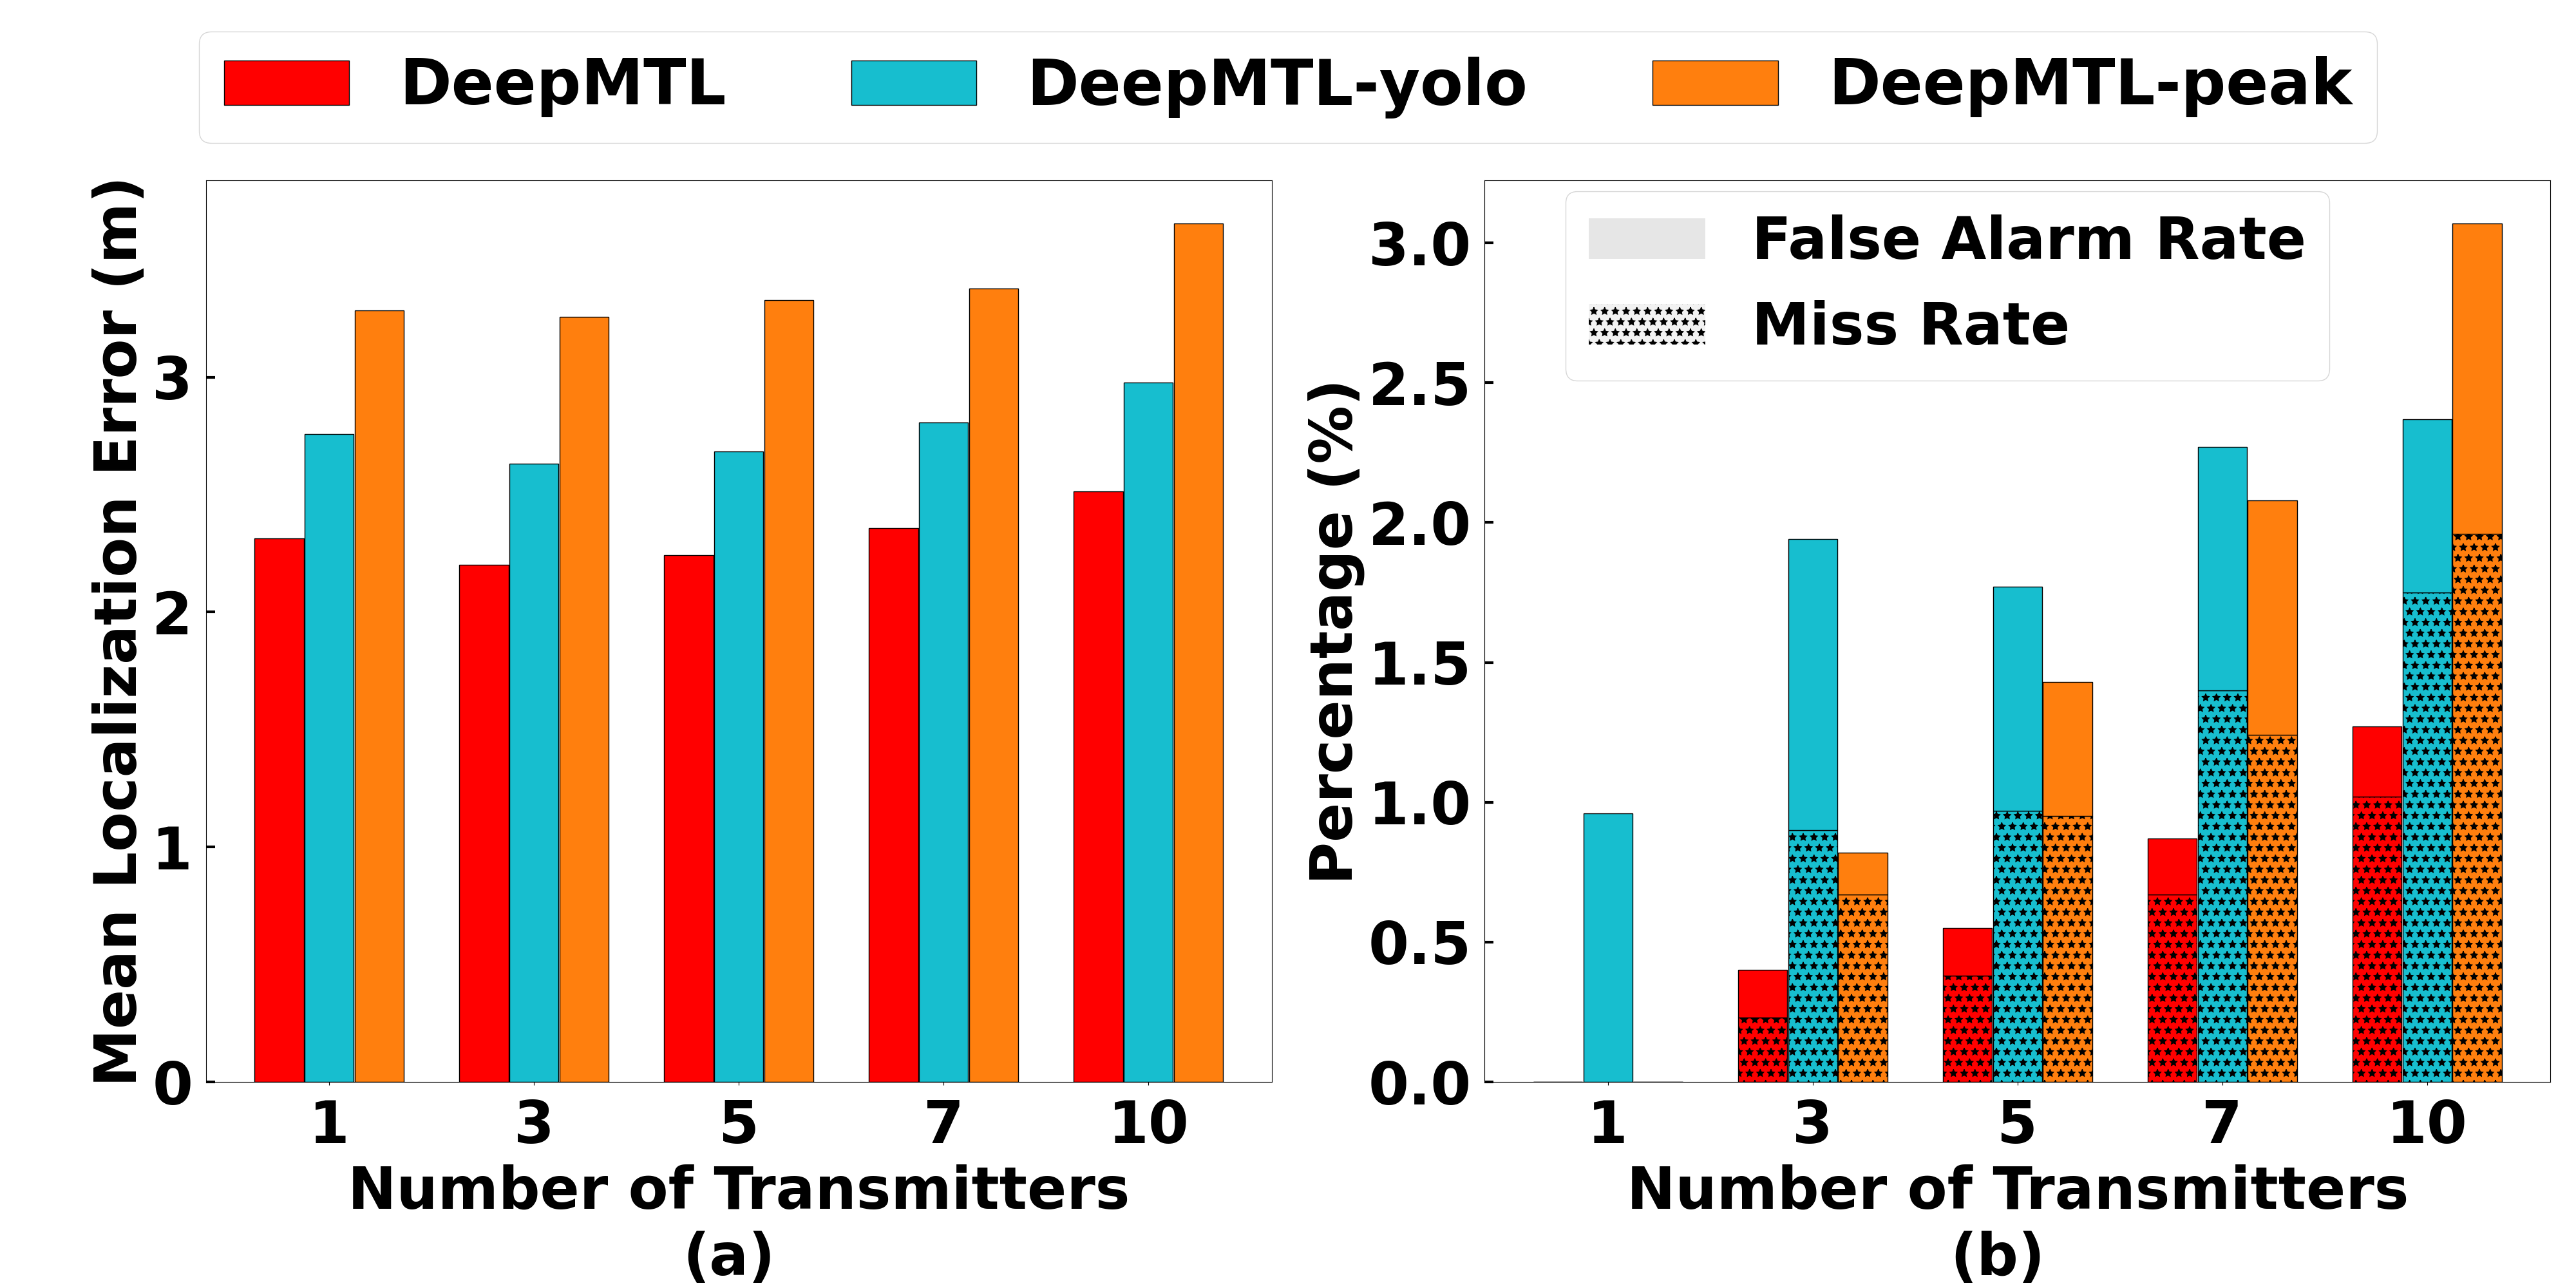
\includegraphics[width=0.75\textwidth]{chapters/wowmom-pmc/figures/ours_error_missfalse_vary_numintru.png}
	\caption{(a) Localization error and (b) miss and false alarm rates, of \our, \ouryolo and \ourpeak variants for varying number of transmitters in log-distance dataset (propagation) model.}
	\label{fig:ours_vary_numintru}
\end{figure}

\begin{figure}[ht]
	\centering
	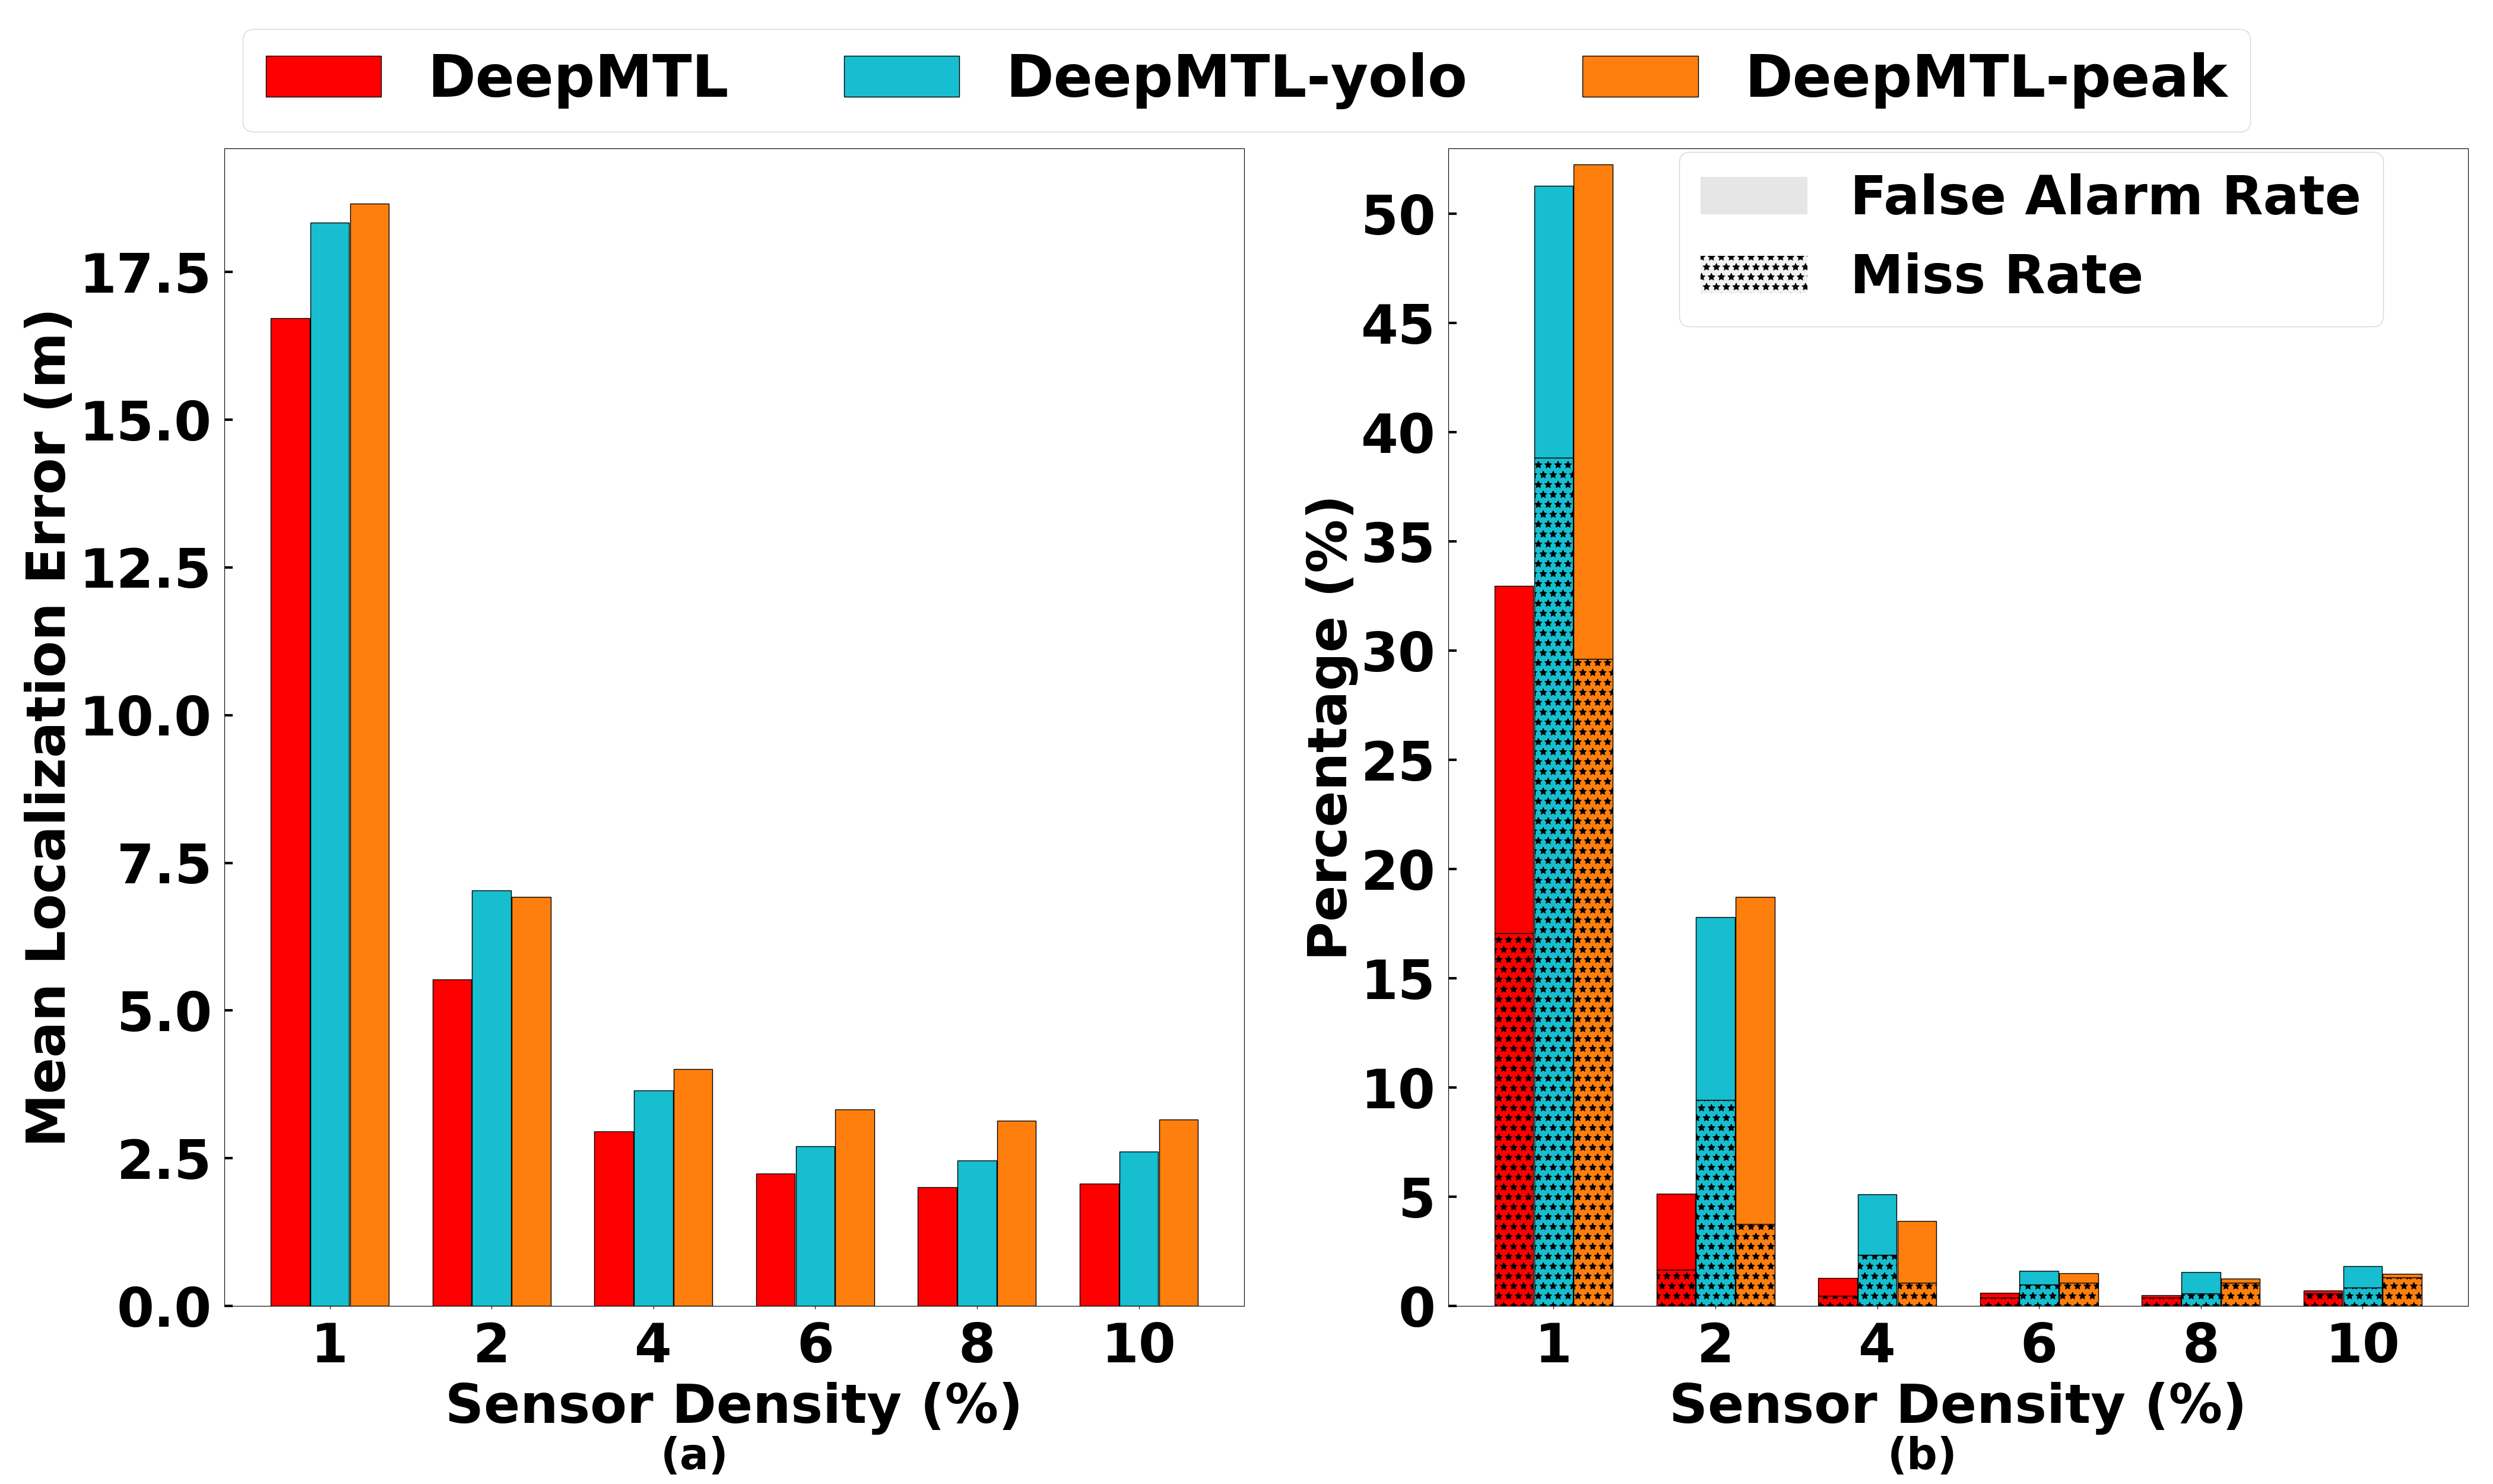
\includegraphics[width=0.75\textwidth]{chapters/wowmom-pmc/figures/ours_error_missfalse_vary_sendensity.png}
	\caption{(a) Localization error and (b) miss and false alarm rates, of \our, \ouryolo and \ourpeak variants for varying sensor density in log-distance dataset (propagation) model.}
	\label{fig:ours_vary_sendensity}
\end{figure}



\subsection{\our vs.\ \ouryolo vs.\ \ourpeak}

In this subsection, we compare the three variants of our technique, viz., \our, \ouryolo, and
\ourpeak. For simplicity, we only show plots for the log-distance propagation model setting in this 
subsection (we observed similar performance trends for the Longley-Rice propagation model too). 
%%%%%%%%%%%%%%%%%%%%%%%%%%%%%

\softpara{Performance Results.}
In Fig.~\ref{fig:ours_cdf}, we plot  the cumulative density function (CDF) of the localization
error, for the simple case of a single transmitter.
We observe that \our outperforms the other variants, as it yields a higher cumulative probability for a lower range of errors.
%%%%%%%%%%%%%%%%%%%
In addition, we evaluate the three variants for varying number of transmitters (Fig.~\ref{fig:ours_vary_numintru}) and sensor density (Fig.~\ref{fig:ours_vary_sendensity}), and evaluate the localization error as well as the false alarm and miss rates. 
%%%%%%%%%%%%%%%%
We observe that \our consistently outperforms the other two variants 
across all plots and performance metrics. As expected, the performance of all algorithms 
degrades with an increase in the number of transmitters (in terms of false alarms and miss rates) or with a decrease in sensor density. 
In general, the localization error of \our is around 15-30\% lower than the other variants.
Impressively, the total cardinality error (i.e., false alarms plus miss rates) is fewer than 1\% for the \our technique, when the sensor density is 6\% or above.

When the sensor density is as low as 1\%, the performance of all methods significantly decreases.
Because when the sensor density is 1\% or lower, the input image will be very sparse and contain only a few pixels.
\our's first part \imgimg has a receptive field of $17\times17$.
This area will contain an average of less than three sensors when the sensor density is 1\% ($17\times17\times0.01=2.89$).
This number is considered too low and note that 2.89 sensors are not enough for the trilateration localization method, which needs three sensors.
Our CNN models need to function well with enough pixels that contain useful information. 
So we suggest the sensor density to be at least 2\% to achieve reasonable results.

\begin{table}[ht]
	\centering
	\caption{Compare Localization Running Time (s) for 1 to 10 Number of Intruders}
	\vspace{-0.1in}
	\begin{tabular}{c c c c c c c}
		\hline\hline
		\small{Intru.} & \small{\ourpeak}  & \small{\ouryolo} & \small{\our} & \small{\map} & \small{\splot} & \small{\deeptx} \\
		\hline
		1 & 0.0013 & 0.0180 & 0.0180 & 8.78 & 1.53 & 0.0015 \\ 
		3 & 0.0014 & 0.0183 &  0.0186 & 15.1 & 1.79 & 0.0016 \\
		5 & 0.0016 & 0.0192 &  0.0189 & 19.3 & 2.06 & 0.0017\\
		7 & 0.0018 & 0.0196 &  0.0194 & 24.1 & 2.32 & 0.0019 \\
		10 & 0.0023 & 0.0205 & 0.0206 & 28.5 & 2.72 & 0.0022 \\
		\hline
	\end{tabular}
	\label{table:running-time}	
\end{table}


\softpara{Running Time Comparison.} For the running time comparison of the variants, see Table \ref{table:running-time}. 
Our hardware is an Intel i7-8700 CPU and an Nvidia RTX 2070 GPU. 
We observe that, as expected, \our and \ouryolo which use a sophisticated object-detection method do incur higher latency (around 20 milliseconds) than \ourpeak (around two milliseconds). As our key
performance criteria is accuracy and the run time of \our is still quite low, we choose \our for comparison with the prior works in ~\S\ref{subsec:vs_prior}. 


\softpara{Localizing Transmitters Close By.}
Localizing two or more transmitters close by is a hard part of the \mtl problem.
Fig.~\ref{fig:peaks}(c) and (d) gives an example of when an advanced object detection algorithm will work while a simple local maximal peak detection might not.
Fig.~\ref{fig:peaks}(c) and (d) shows \our can successfully localize two transmitters as close as three pixels apart.
When a pixel represents a $10m \times 10m$ area, then it is 30 meters apart.
If a pixel represents a smaller area, such as $1m \times 1m$, it has the potential to localize two transmitters as close as three meters apart.

\softpara{Two YOLO Thresholds.} YOLO has two important thresholds to tune that can affect the miss rate and false alarm rate. 
One is the confidence threshold (\conf) and the other is the non-maximum suppression threshold (\nms).
An object will be recognized as a peak only if its confidence level is larger than \conf.
If two recognized peaks' bounding boxes have a large overlap, and their intersection of union is higher than \nms, then the two peaks will be considered as one peak. 
The peak with a higher confidence level keeps while the other peak with a lower confidence level discards.
A higher \conf will bring a lower false alarm rate but a higher miss rate, and a higher \nms will bring a lower miss rate but a higher false alarm rate.
We pick \conf= 0.8 and \nms= 0.5 for \our as we observe these values bring a good balance between false alarm rate and miss rate.
In particular, a high \conf of 0.8  precludes ``fake peaks" at locations with no transmitters.
Also, a low \nms weakens \our's ability to localize two close by transmitters, while a high $nms$ yields
a high false alarm rate (by incorrectly interpreting a single transmitter as multiple close by transmitters); thus, we chose \nms of 0.5.


% \begin{figure}[h]
% 	\centering
% 	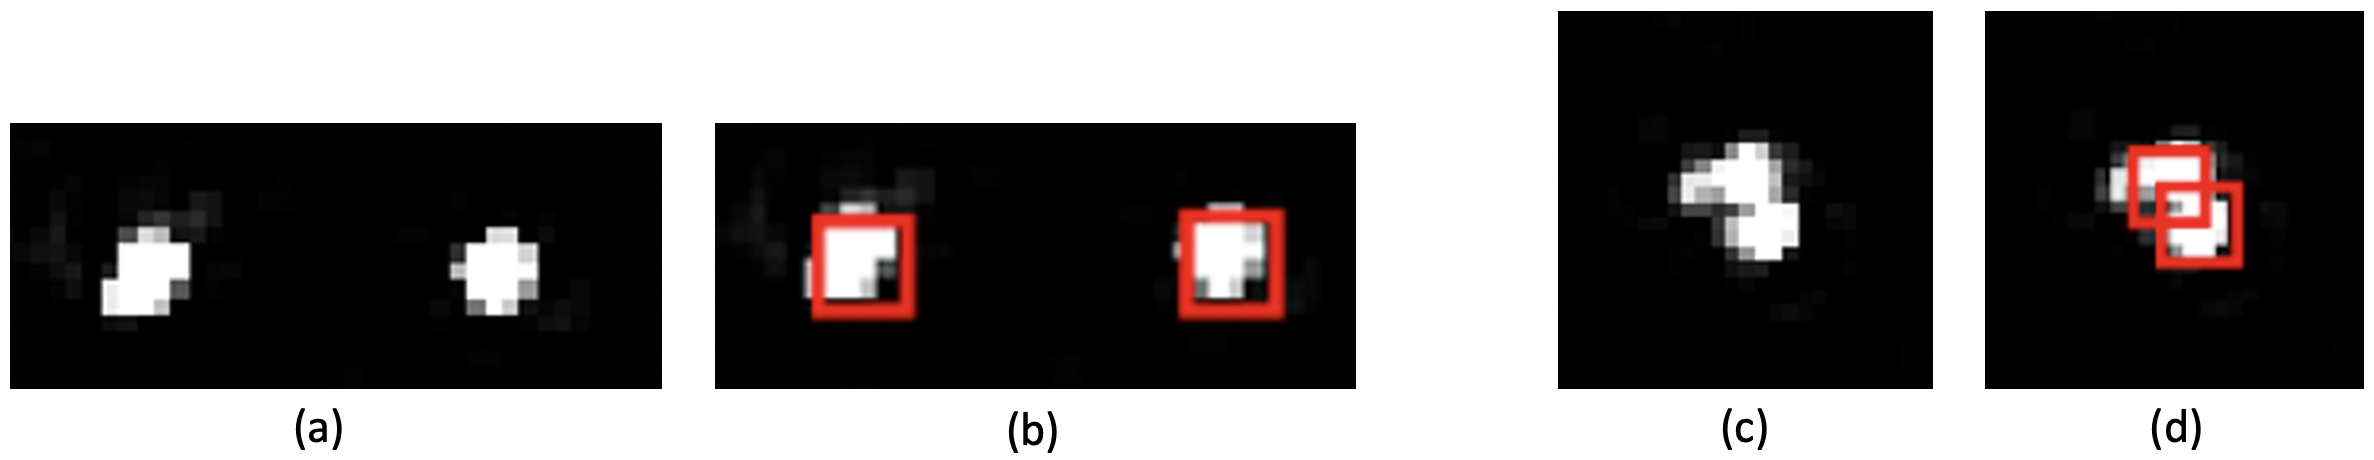
\includegraphics[width=0.3\textwidth]{chapters/wowmom-pmc/figures/peaks.png}
% 	\caption{A zoom-in of two close peaks in Fig. \ref{fig:overall} (b). A clearer understanding of the mechanisms the \imgimg and \yolocust.}
% 	\label{fig:peaks}
% \end{figure}


\subsection{\our vs.\ Prior Works}
\label{subsec:vs_prior}
%%%%%%% comparing 4 $$$$$$$$$$$$

\begin{figure}[t]
	\centering
	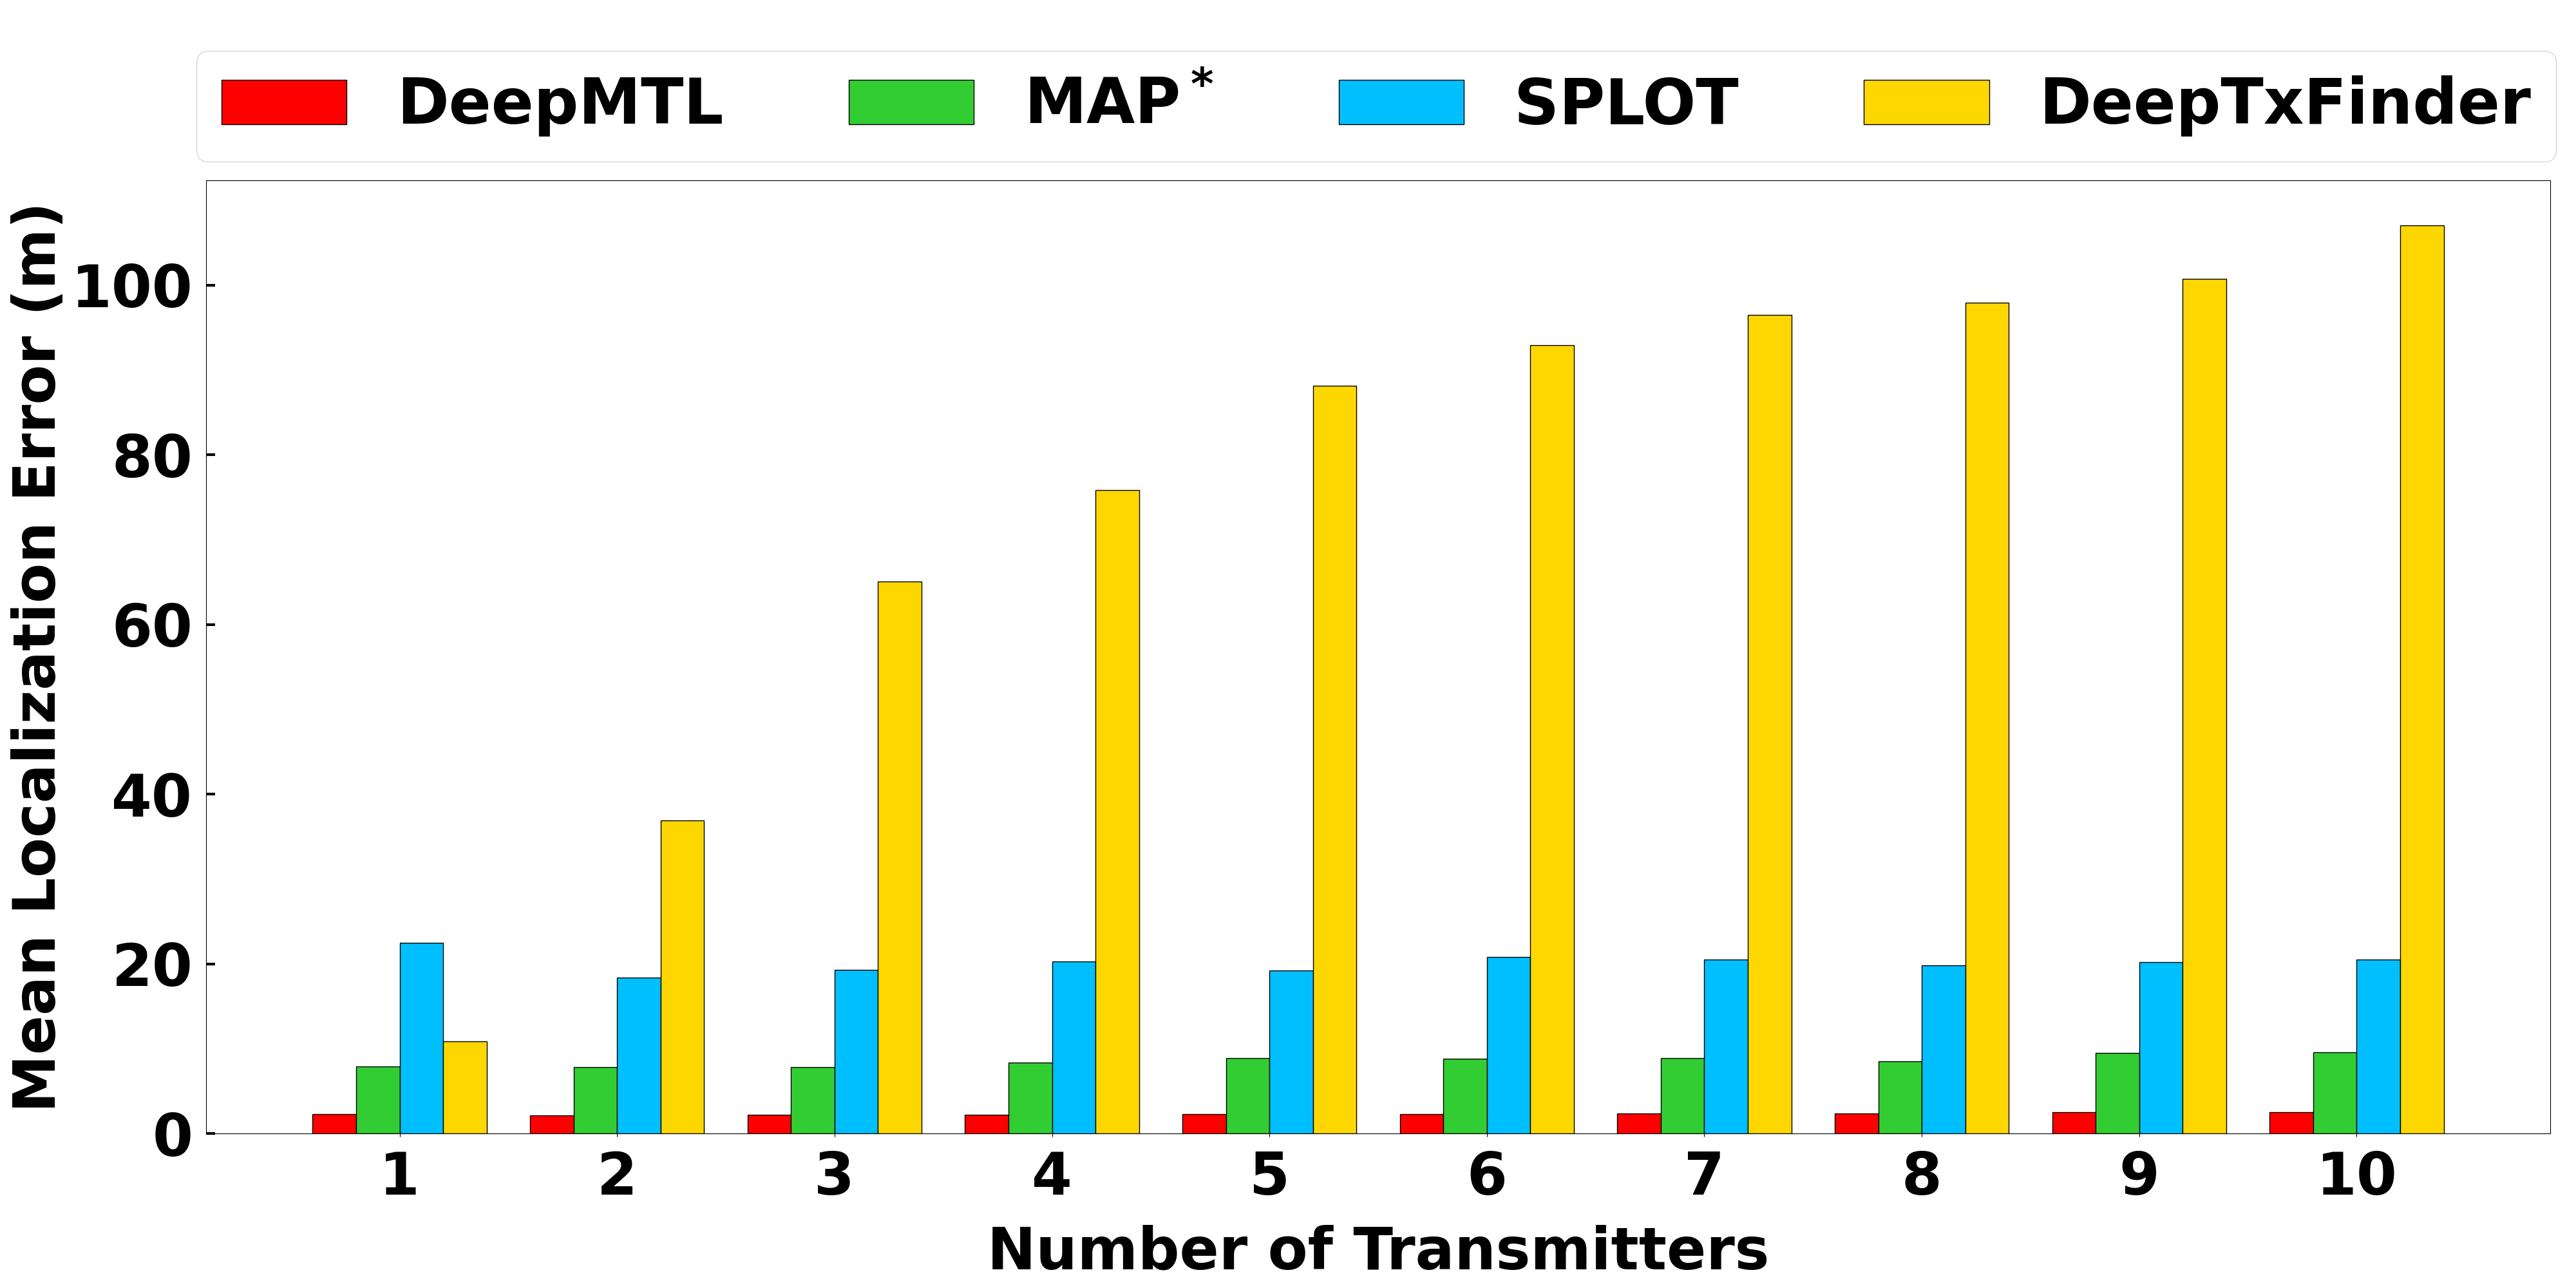
\includegraphics[width=0.75\textwidth]{chapters/wowmom-pmc/figures/log_distance-error_vary_numintru.png}
	\caption{Localization error of \our, \map, \splot, and \deeptx for varying number of transmitters in the log-distance dataset.}
	\label{fig:logdist-error-vary_numintru}
\end{figure}



\begin{figure}[t]
	\centering
	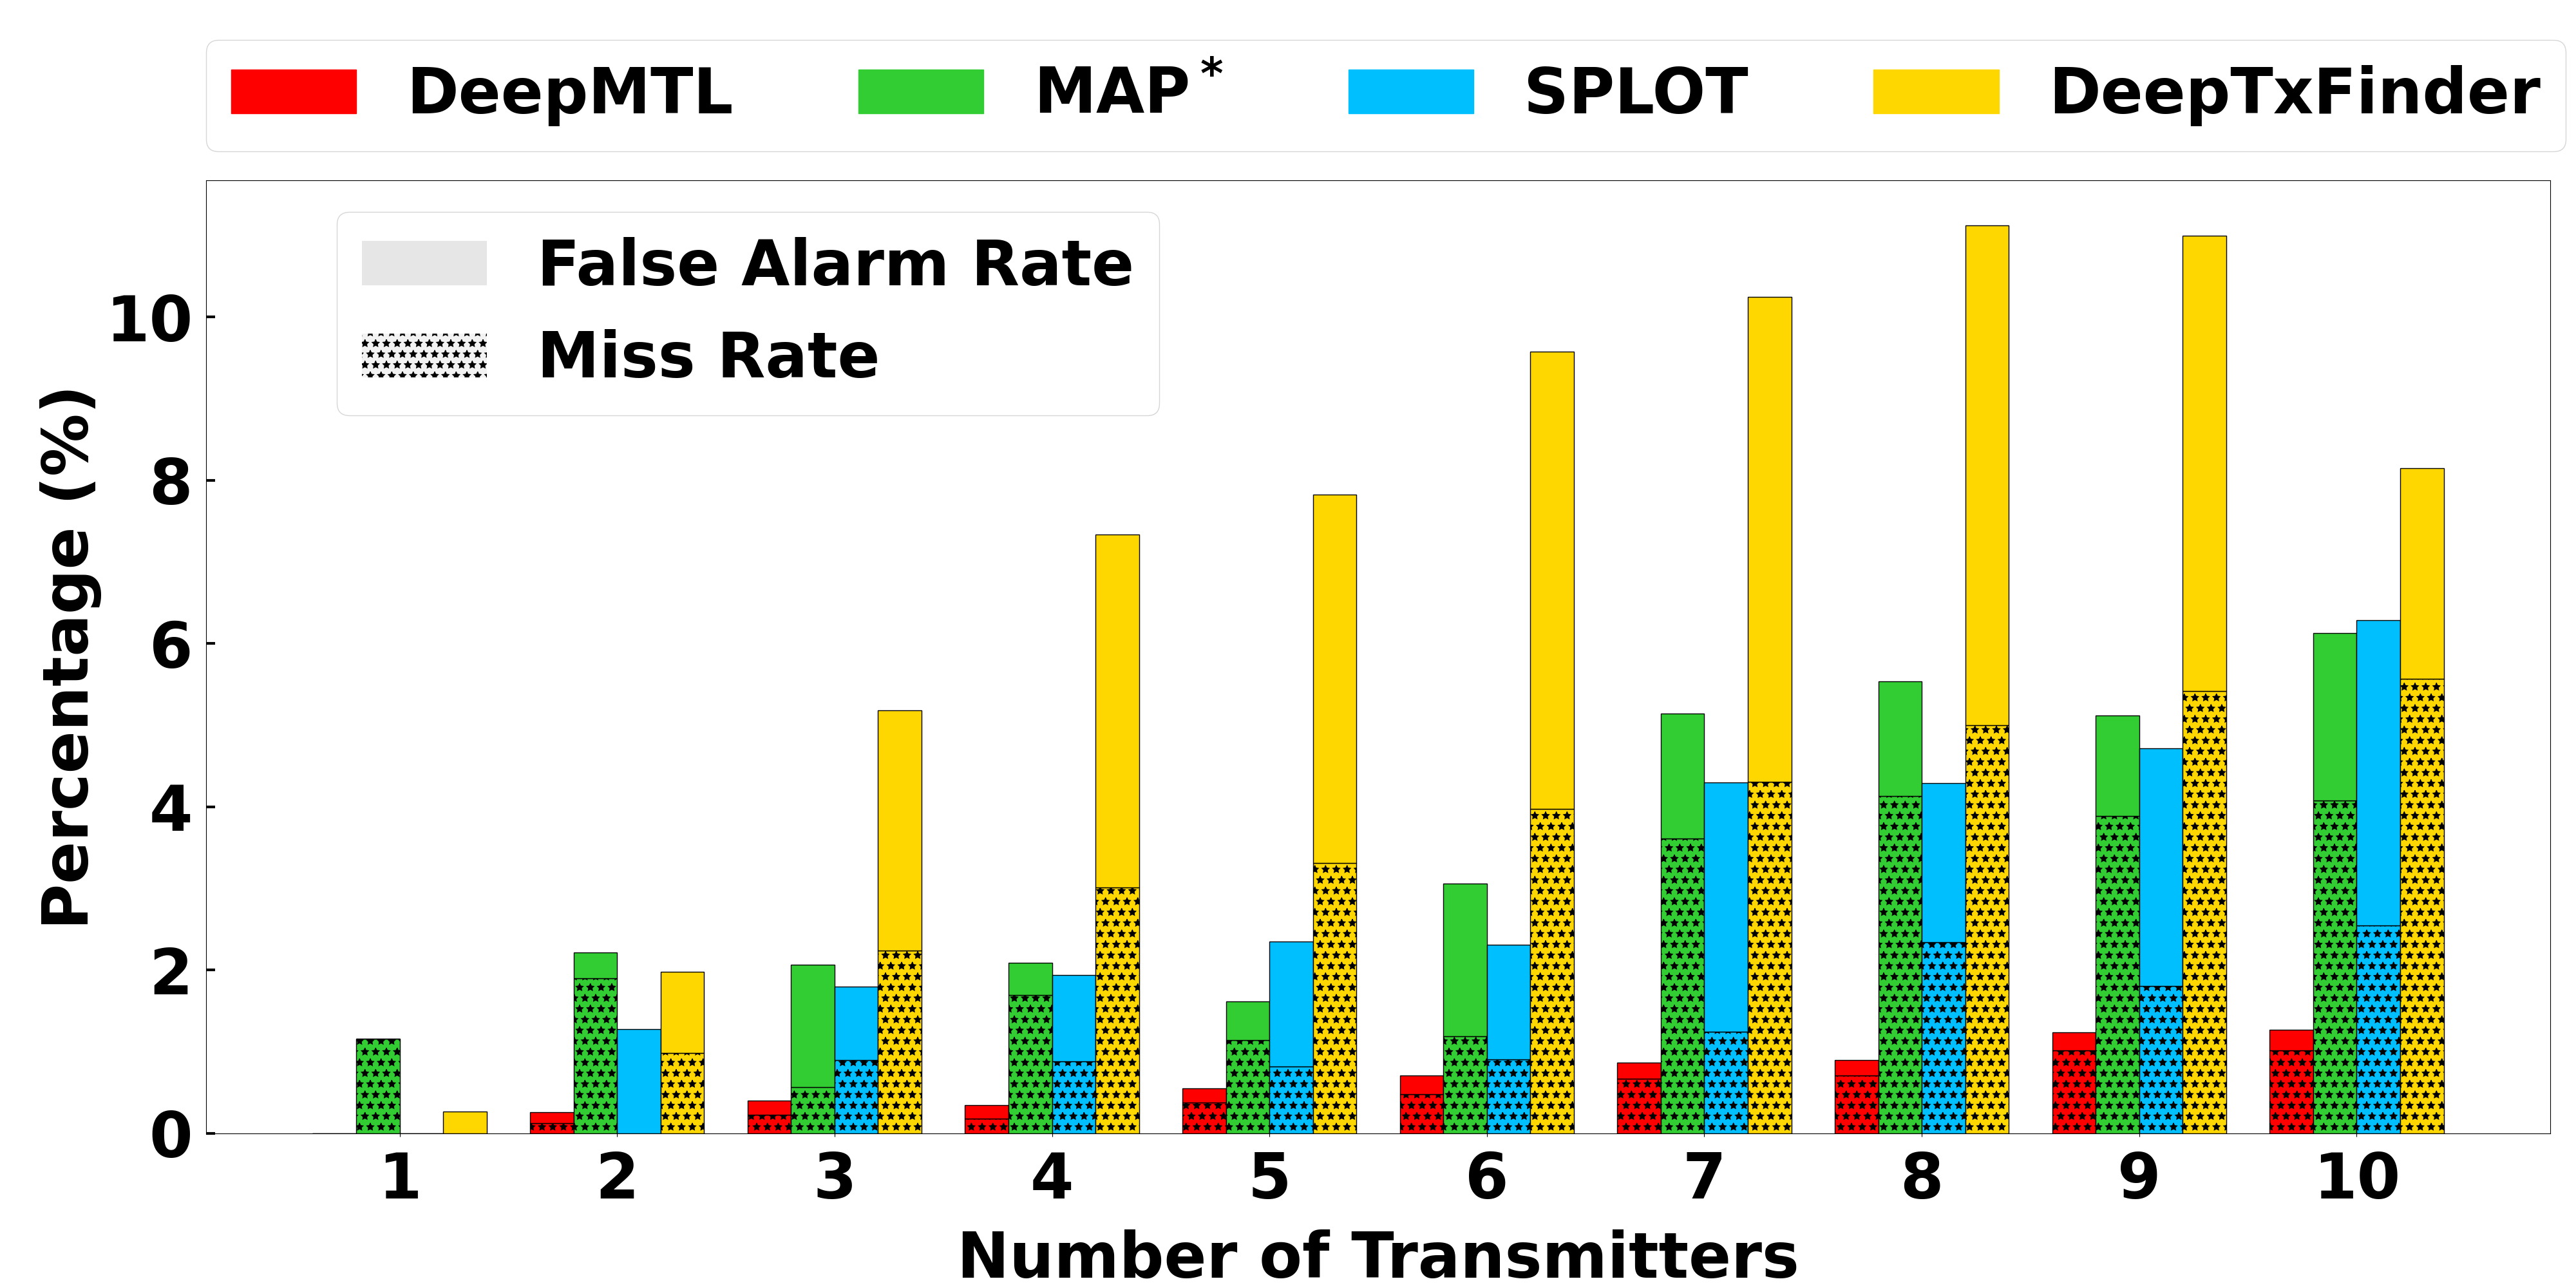
\includegraphics[width=0.75\textwidth]{chapters/wowmom-pmc/figures/log_distance-missfalse_vary_numintru.png}
	\caption{Miss and false alarm rates of \our, \map, \splot, and \deeptx for varying number of transmitters in the log-distance dataset.}
	\label{fig:logdist-missfalse-vary-numintru}
\end{figure}


\begin{figure}[t]
	\centering
	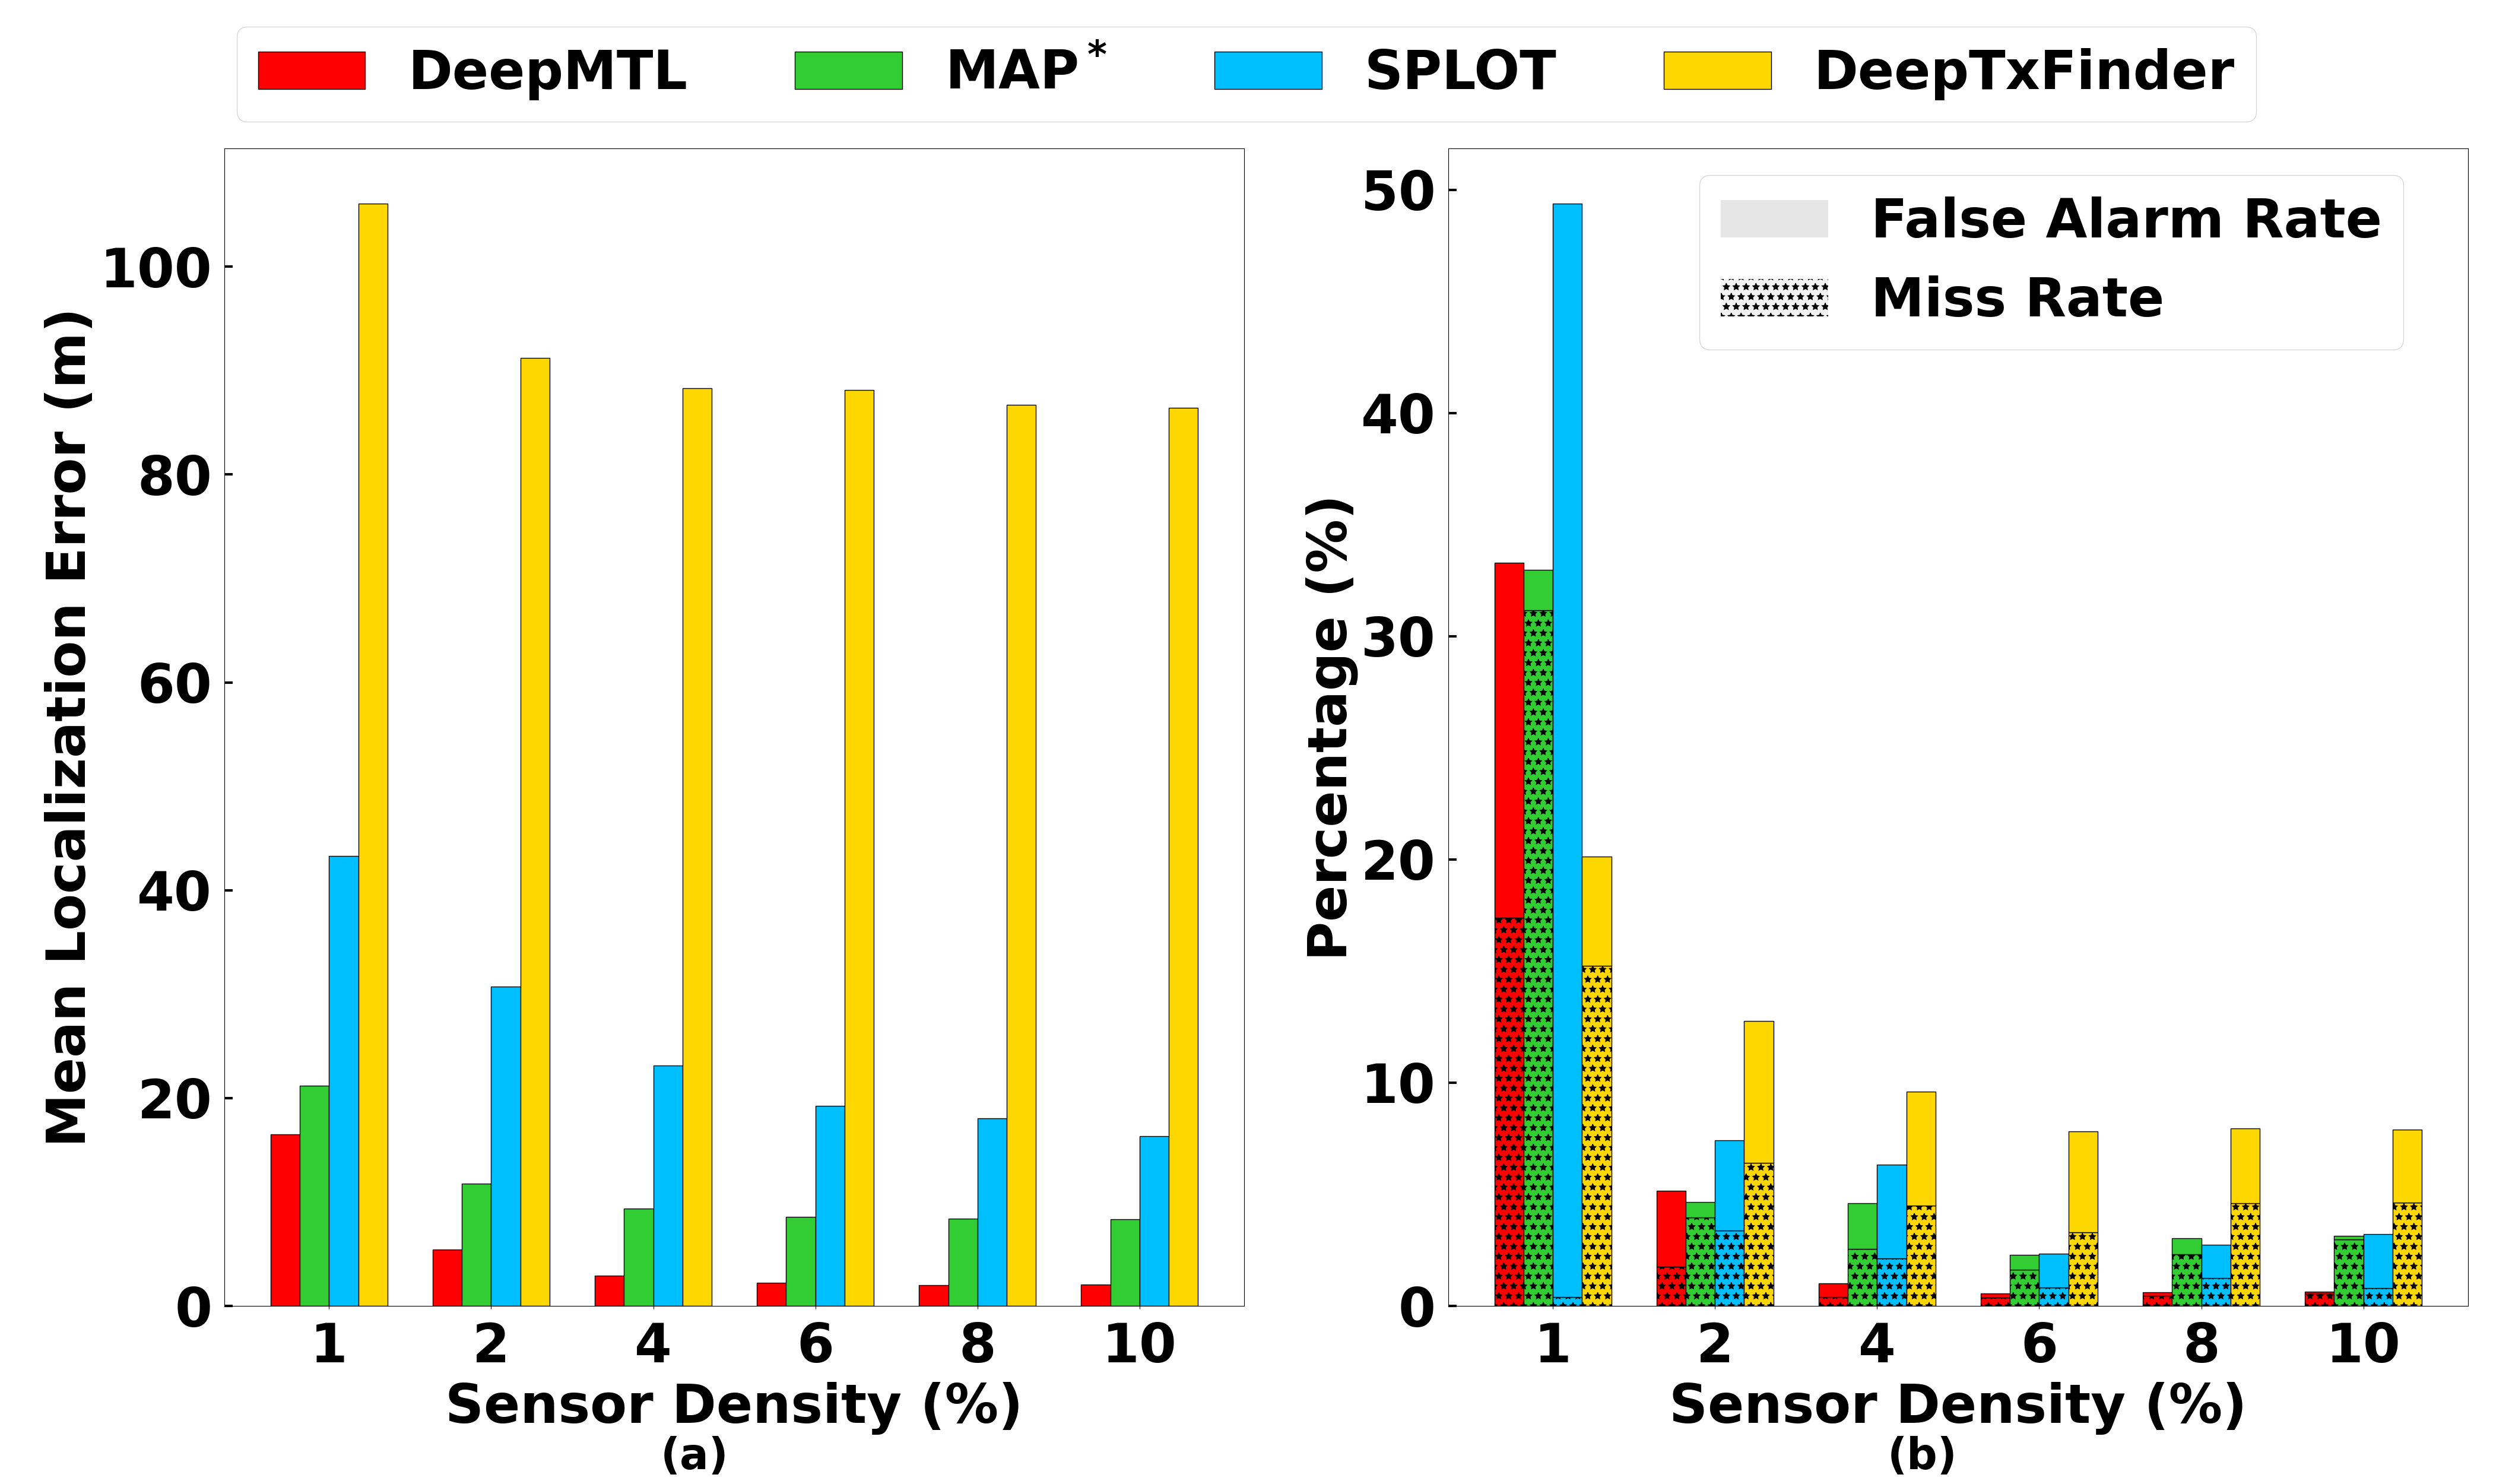
\includegraphics[width=0.75\textwidth]{chapters/wowmom-pmc/figures/log_distance-error_missfalse_vary_sendensity.png}
	\caption{(a) Localization error, and (b) miss and false alarm rates, of \our, \map, \splot, and \deeptx for varying sensor densities in the log-distance dataset.}
	\label{fig:logdist-error_missfalse-vary-sendensity}
\end{figure}





%%%%%%%%%%%%% splat %%%%%%%%%%%%%

\begin{figure}[ht]
	\centering
	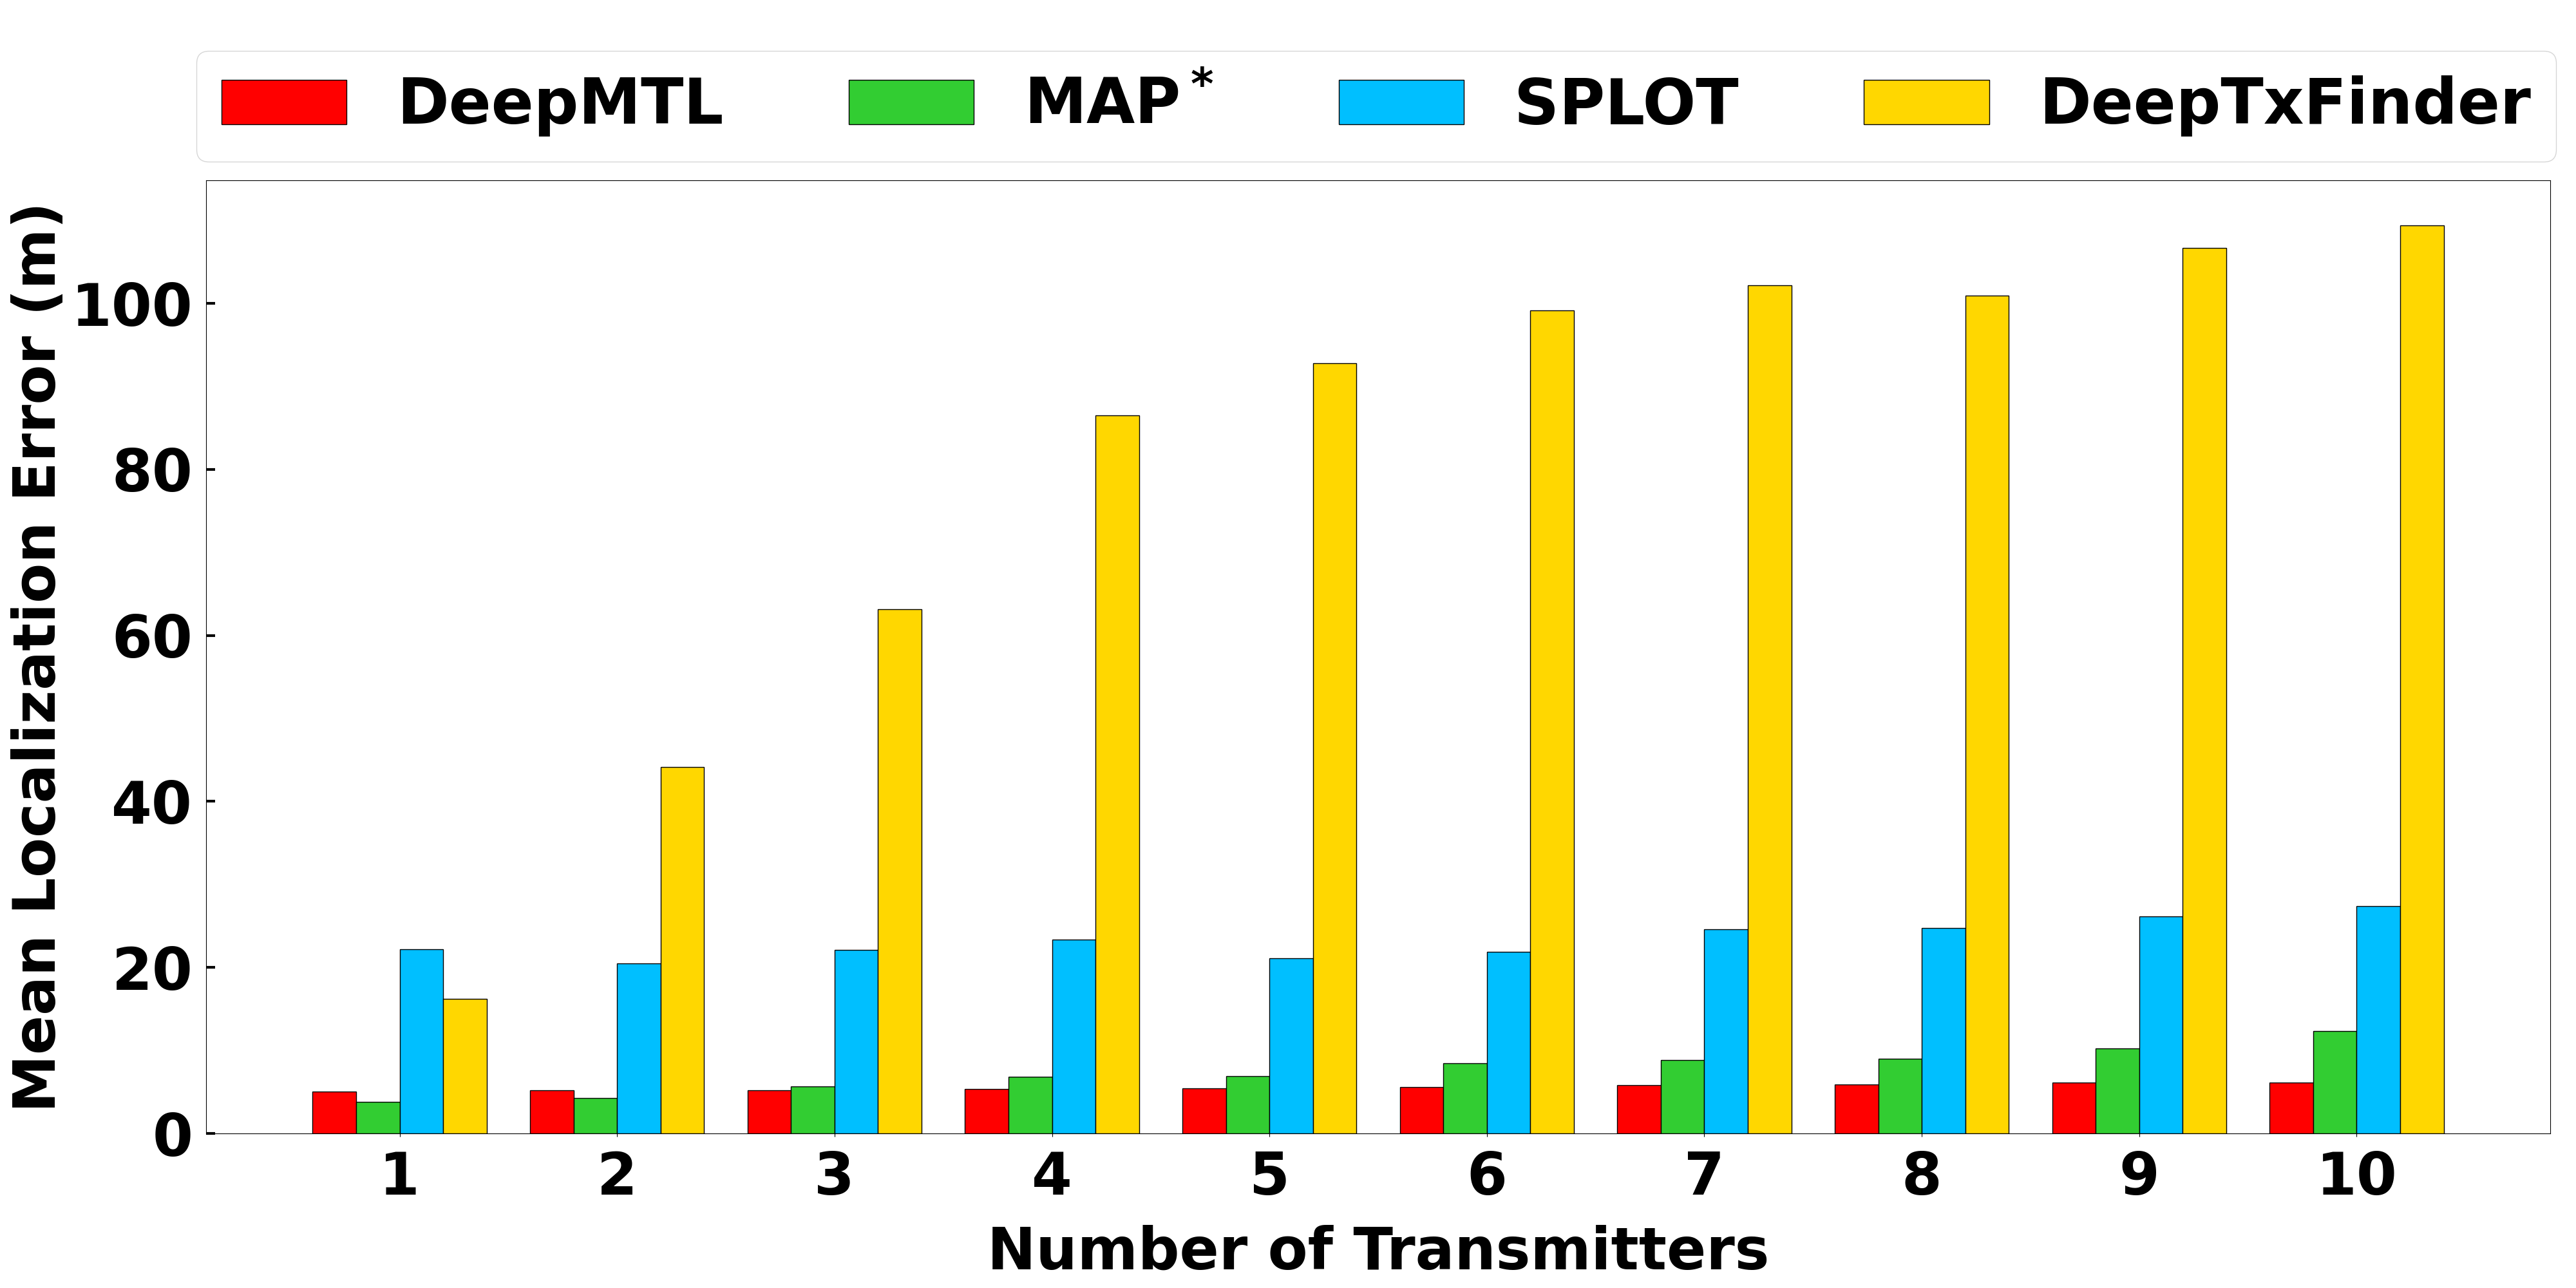
\includegraphics[width=0.75\textwidth]{chapters/wowmom-pmc/figures/splat-error_vary_numintru.png}
	\caption{Localization error of \our, \map, \deeptx and \splot for varying number of transmitters in the SPLAT! Dataset. }
	\label{fig:splat-error-vary_numintru}
\end{figure}

\begin{figure}[ht]
	\centering
	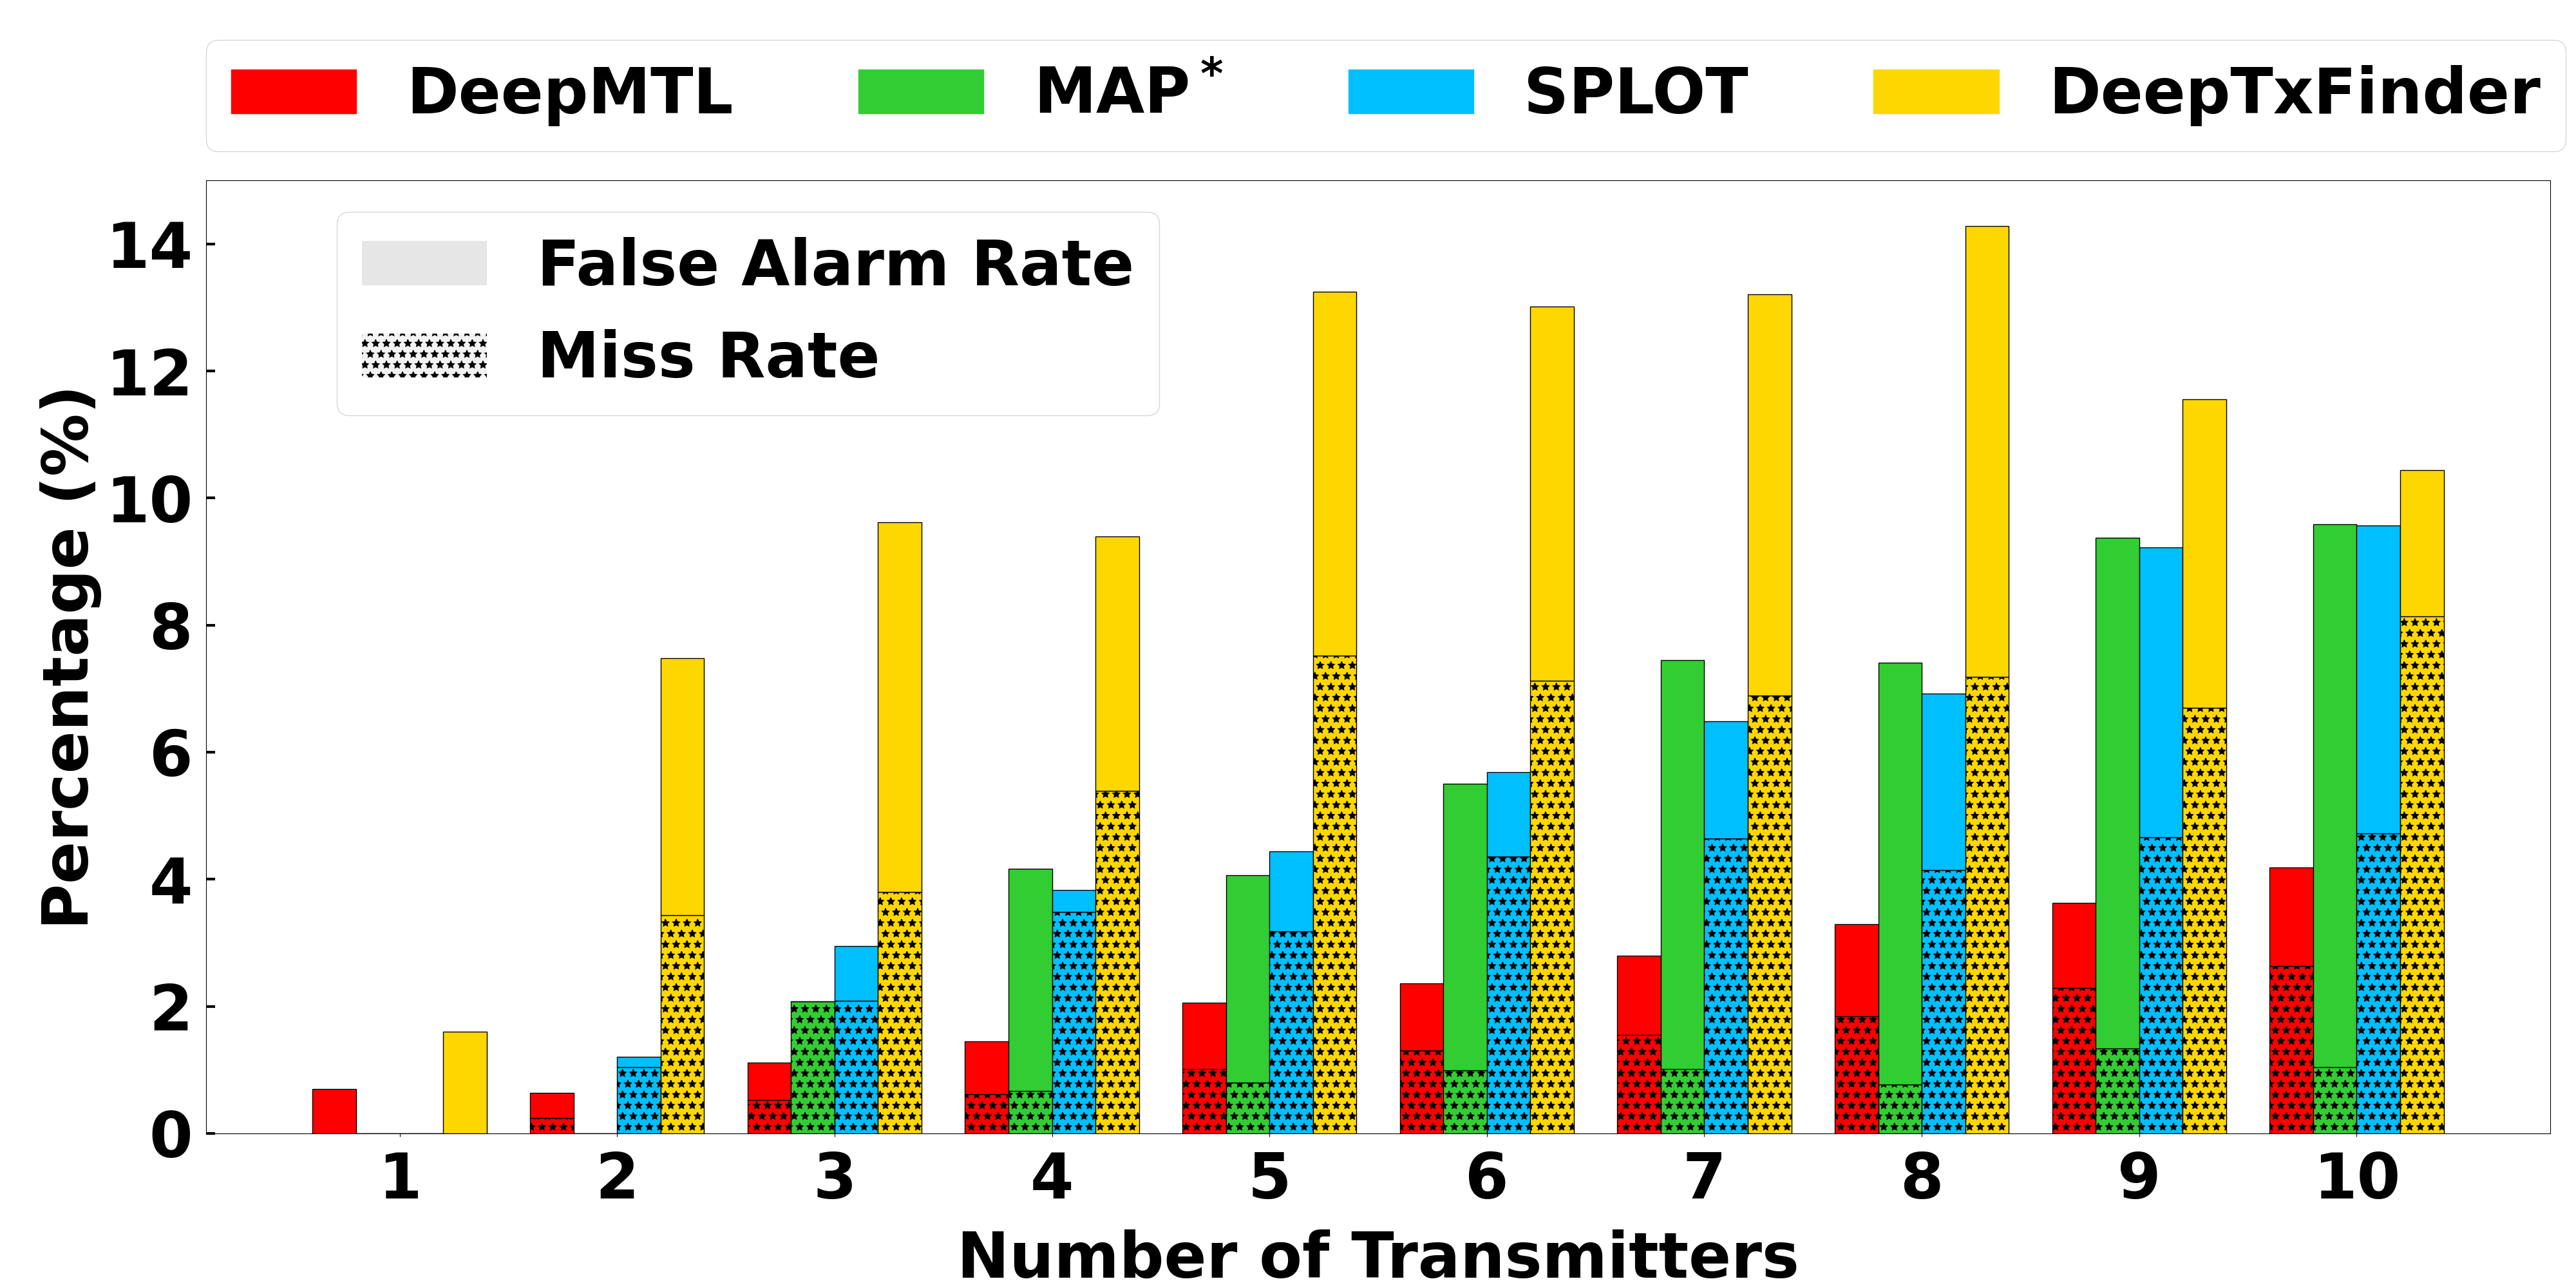
\includegraphics[width=0.75\textwidth]{chapters/wowmom-pmc/figures/splat-missfalse_vary_numintru.png}
	\caption{Miss and false alarm rates of \our, \map, \splot, and \deeptx for varying number of transmitters in the SPLAT! Dataset.}
	\label{fig:splat-missfalse-vary-numintru}
\end{figure}


\begin{figure}[ht]
	\centering
	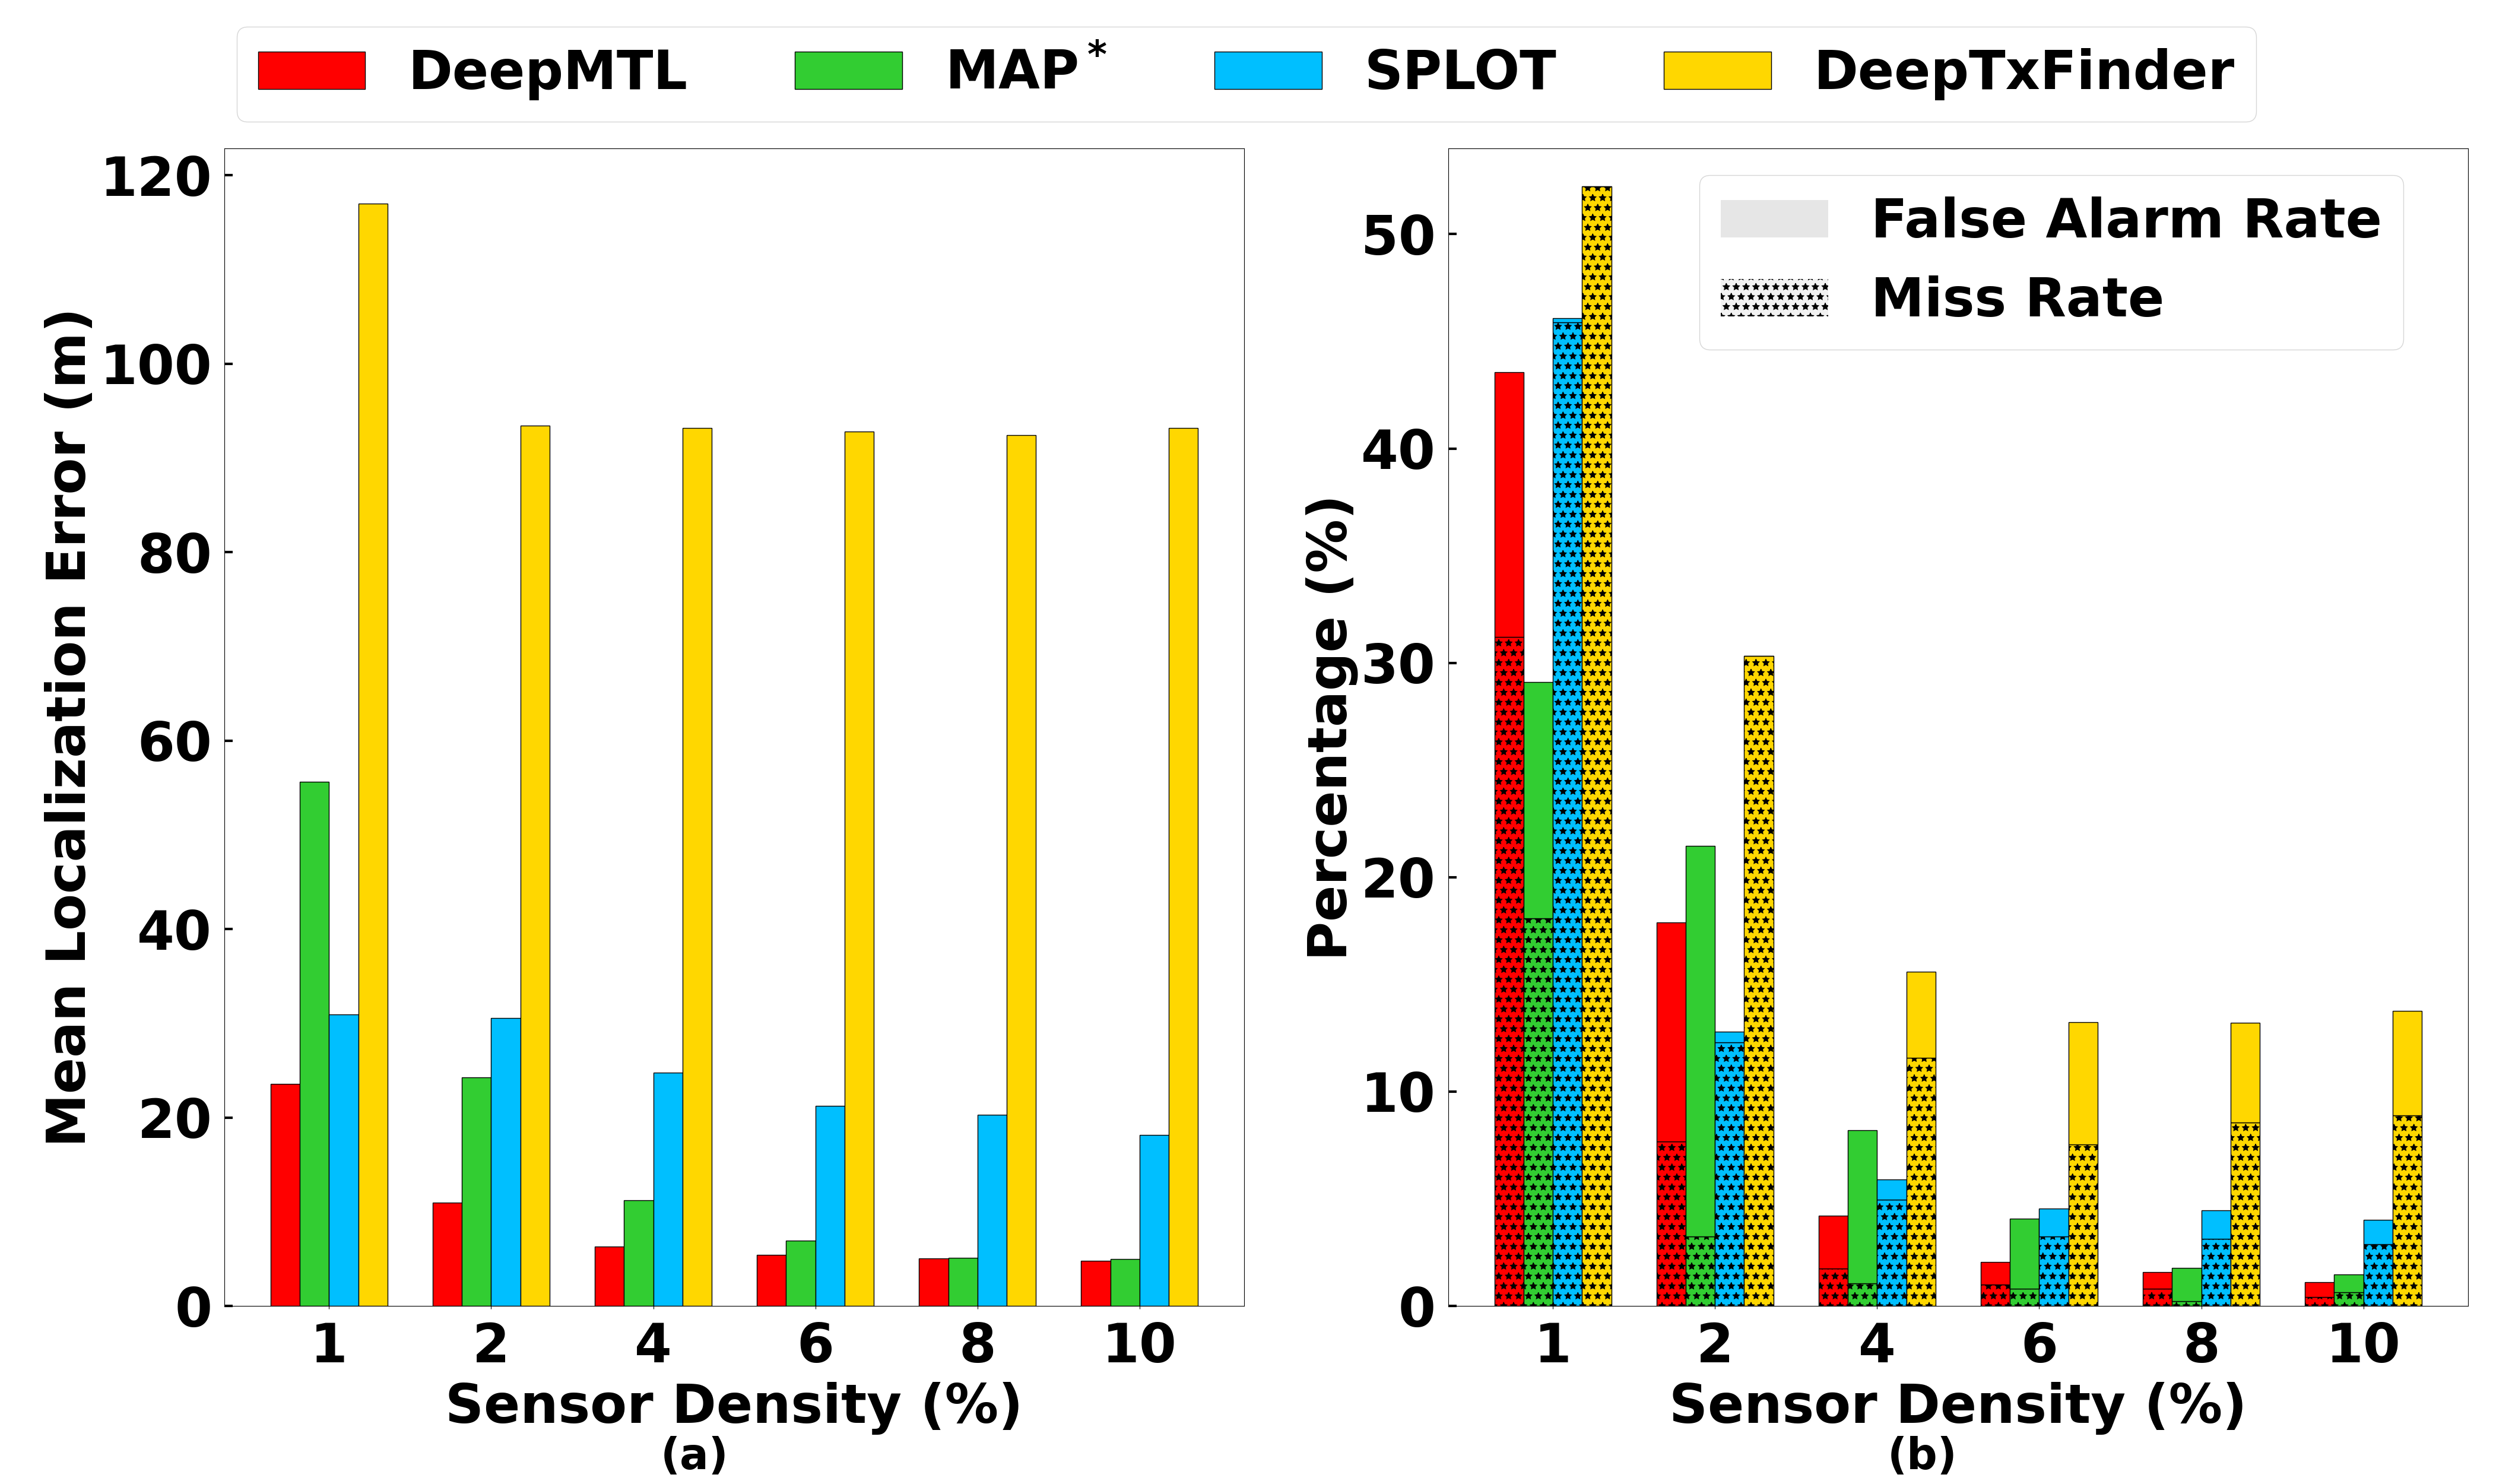
\includegraphics[width=0.75\textwidth]{chapters/wowmom-pmc/figures/splat-error_missfalse_vary_sendensity.png}
	\caption{(a) Localization error, and (b) miss and false alarm rates, of \our, \map, \splot, and \deeptx for varying sensor densities in the SPLAT! Dataset.}
	\label{fig:splat-error-vary-sendensity}
\end{figure}



In this subsection, we compare \our with \splot, \map, \deeptx in both log-distance (Fig.~\ref{fig:logdist-error-vary_numintru}, \ref{fig:logdist-missfalse-vary-numintru}, \ref{fig:logdist-error_missfalse-vary-sendensity}) and SPLAT (Fig.~\ref{fig:splat-error-vary_numintru}, \ref{fig:splat-missfalse-vary-numintru}, \ref{fig:splat-error-vary-sendensity}) propagation models and thus, datasets.
We observe similar performance trends for both datasets, i.e., 
\our significantly outperforms the other approaches by a large margin (in many cases, by more
than 50\% in localization errors, false alarms, and miss rates). For all techniques, as expected,
the performance is generally worse in the SPLAT dataset compared to the log-distance dataset.
%%%%%%%%%%%%%%%%

\softpara{Varying Number of Transmitters.}
Fig.~\ref{fig:logdist-error-vary_numintru} and Fig.~\ref{fig:splat-error-vary_numintru} show the localization error with varying number of transmitters, in the two datasets. We see that \our has a mean localization error of only 2 to 2.5 meters (roughly, one-fourth of the side length of a pixel/grid cell) in the log-distance dataset and about 5 to 6 meters in the SPLAT dataset. In comparison, the
localization errors of \map, \splot, \deeptx are two to three times, eight to nine times, and 
few tens of times respectively more than that of \our. 
%%%%%%%%%%%%%%%%%%%%%%%%%%%%%%%%%%%%%%%
Fig.~\ref{fig:logdist-missfalse-vary-numintru} and Fig.~\ref{fig:splat-missfalse-vary-numintru} show the miss and false alarm rates with varying number of transmitters in the two datasets.
We observe that \our's summation of miss and false alarm rate is only 1\% even at 
ten transmitters in the log-distance dataset, and about 4\% for the case of \splat dataset. 
In comparison, the summation of miss and false alarm rates for other schemes is at least 6\% and
10\% respectively for the two datasets, when there are ten transmitters.

\softpara{Varying Sensor Density.}
Fig.~\ref{fig:logdist-error_missfalse-vary-sendensity} and Fig.~\ref{fig:splat-error-vary-sendensity} plot the performance of various algorithms for varying sensor density in the two datasets. For very low sensor density of 1\%, all algorithms perform 
badly (in comparison with higher sensor densities), but \our still performs the best except that \map performs best at 1\% in terms of false alarm rate and miss rate.
For higher sensor densities, we observe a similar performance trend as above---i.e., \our easily outperforms the other schemes by a large margin.
For the SPLAT! dataset at the 6\% sensor density, the summation of false alarm rate and miss rate is 2\%, which is higher than the 1\% summation for the log-distance dataset.

\softpara{Running Times.}
The run time of \our (in tens of milliseconds) is orders of magnitude faster than \map and \splot (both in seconds). 
See Table \ref{table:running-time}. 
The \our run time is an order of magnitude slower than \deeptx (in a few milliseconds), due to the deep \yolocust taking up over 90\% of the run time.


\softpara{Summary and Analysis}. 
In summary, our approach significantly outperforms the other approaches in all the accuracy performance metrics, as well as in terms of latency. 
In particular, our approach also significantly outperforms the other CNN-based approach \deeptx. 
The main reason for \deeptx's inferior performance is its inability to accurately predict the number of TXs---which 
forms a fundamental component of their technique. In contrast, \our can circumvent explicit pre-prediction
of number of transmitters by using a well-developed object-detection technique which works well for multiple objects 
especially in our context of simple objects.
%%%%%%%%%


%\blue{We observe \deeptx is performing bad mainly because it cannot predict the number of the TX accurately. 
%The inaccuracy in predicting the number of TX will later affect predicting the location of TX negatively. 
%The advantage here for \our is that the \yolocust is able to take care of the multiple transmitters elegantly through advanced %computer vision techniques. 

%Note that we tried to enhance the CNN model that predicts the number of TX. 

%The overall performance increases but the improvement is not significant. The superiority of \our over \mtl and \splot is because of reframing the wireless localization problem to an image-based problem and resorting to computer vision techniques.}

%how that our approach outperforms the previous approaches 
%significantly (by 50\% or more) in accuracy performance metrics, and incurs an order of magnitude
%less latency compared to other prior works. 

%\begin{enumerate}
%    \item [8 PLOTS] Large scale simulations (100 by 100). Log-distance (?) and Splat. 100 to 1000 sensors (one model). 1 to 10 TXs. Power Range: p plus/minus 5 dB (maybe, plus/minus 10 dB later). PLOTS: Varying # of TXs, # of sensors, # of training images (10k, 20k, 50k, 75k, 100k).
%    \item [4 PLOTS] Testbed Data. IPSN 2020. 1 to 3 TXs. .....   
%    \item Algorithms: Ours (2), IPSN 20, SPLOT, DeepTxFinder.
%    \item Need to bring in training cost comparison across algorithms.
%\end{enumerate}

% \subsection{Large Scale Simulation Dataset}
% Here we simulate the training dataset through a propagation model.


% \subsection{Small Scale Trace Driven Dataset}
% Although simulation is a good metric to pick the best localization algorithm, the better setting is a miniature but realistic experiment using commercial devices.
% Here we use data collected from \cite{ipsn20-mtl} (outdoor). The reason we pick this dataset is it reflects a realistic application of share spectrum system and it gives us the power to change the TXs' configuration (location and power) as it basically provides path-loss values between any arbitrary pair of locations.
% This dataset was collected in area of $32m \times 32m$ with 100 grid cells (each of $3.2m \times 3.2m$).
% We vary number of intruders, deployed sensors, and the number of training samples just what we did for simulations.

% \softpara{Varying Number of Intruders.} We see a similar trend compared to simulations as Figure [] shows. We vary the number of intruders between ... and ...
% We can see that \yolo and \peak can outperform the other algorithms, overall.
% When the number of intruders increases, the performance of the algorithms ....
% As expected, false alarm and miss rate values show that ... has the worst performance while ... shows its strength.
% The performance of ..., among all, shows a consistent behavior meaning ... 


% \softpara{Varying Sensor Density.}
% Now, we try to understand the importance of deployed sensors density.
% We change, due tho small area of interest, from very low number ... to the number as high as ...
% Figure [] simply proves that the higher the number of sensors, the better results we can get for all algorithms.

% \softpara{Varying Training Cost.}
% Finally, we consider the effect of number of training samples on the efficiency of the described algorithms. See Figure [].
% Performance of all algorithms get better when the number of training samples increases. ... performs better when the training samples size is small but ... get much more benefit when this value is moderate.


\subsection{Transfer Learning}
\label{subsec:transfer_learning}

\begin{figure*}[t!]
    \centering
    \begin{subfigure}[t]{0.48\textwidth}
        \centering
        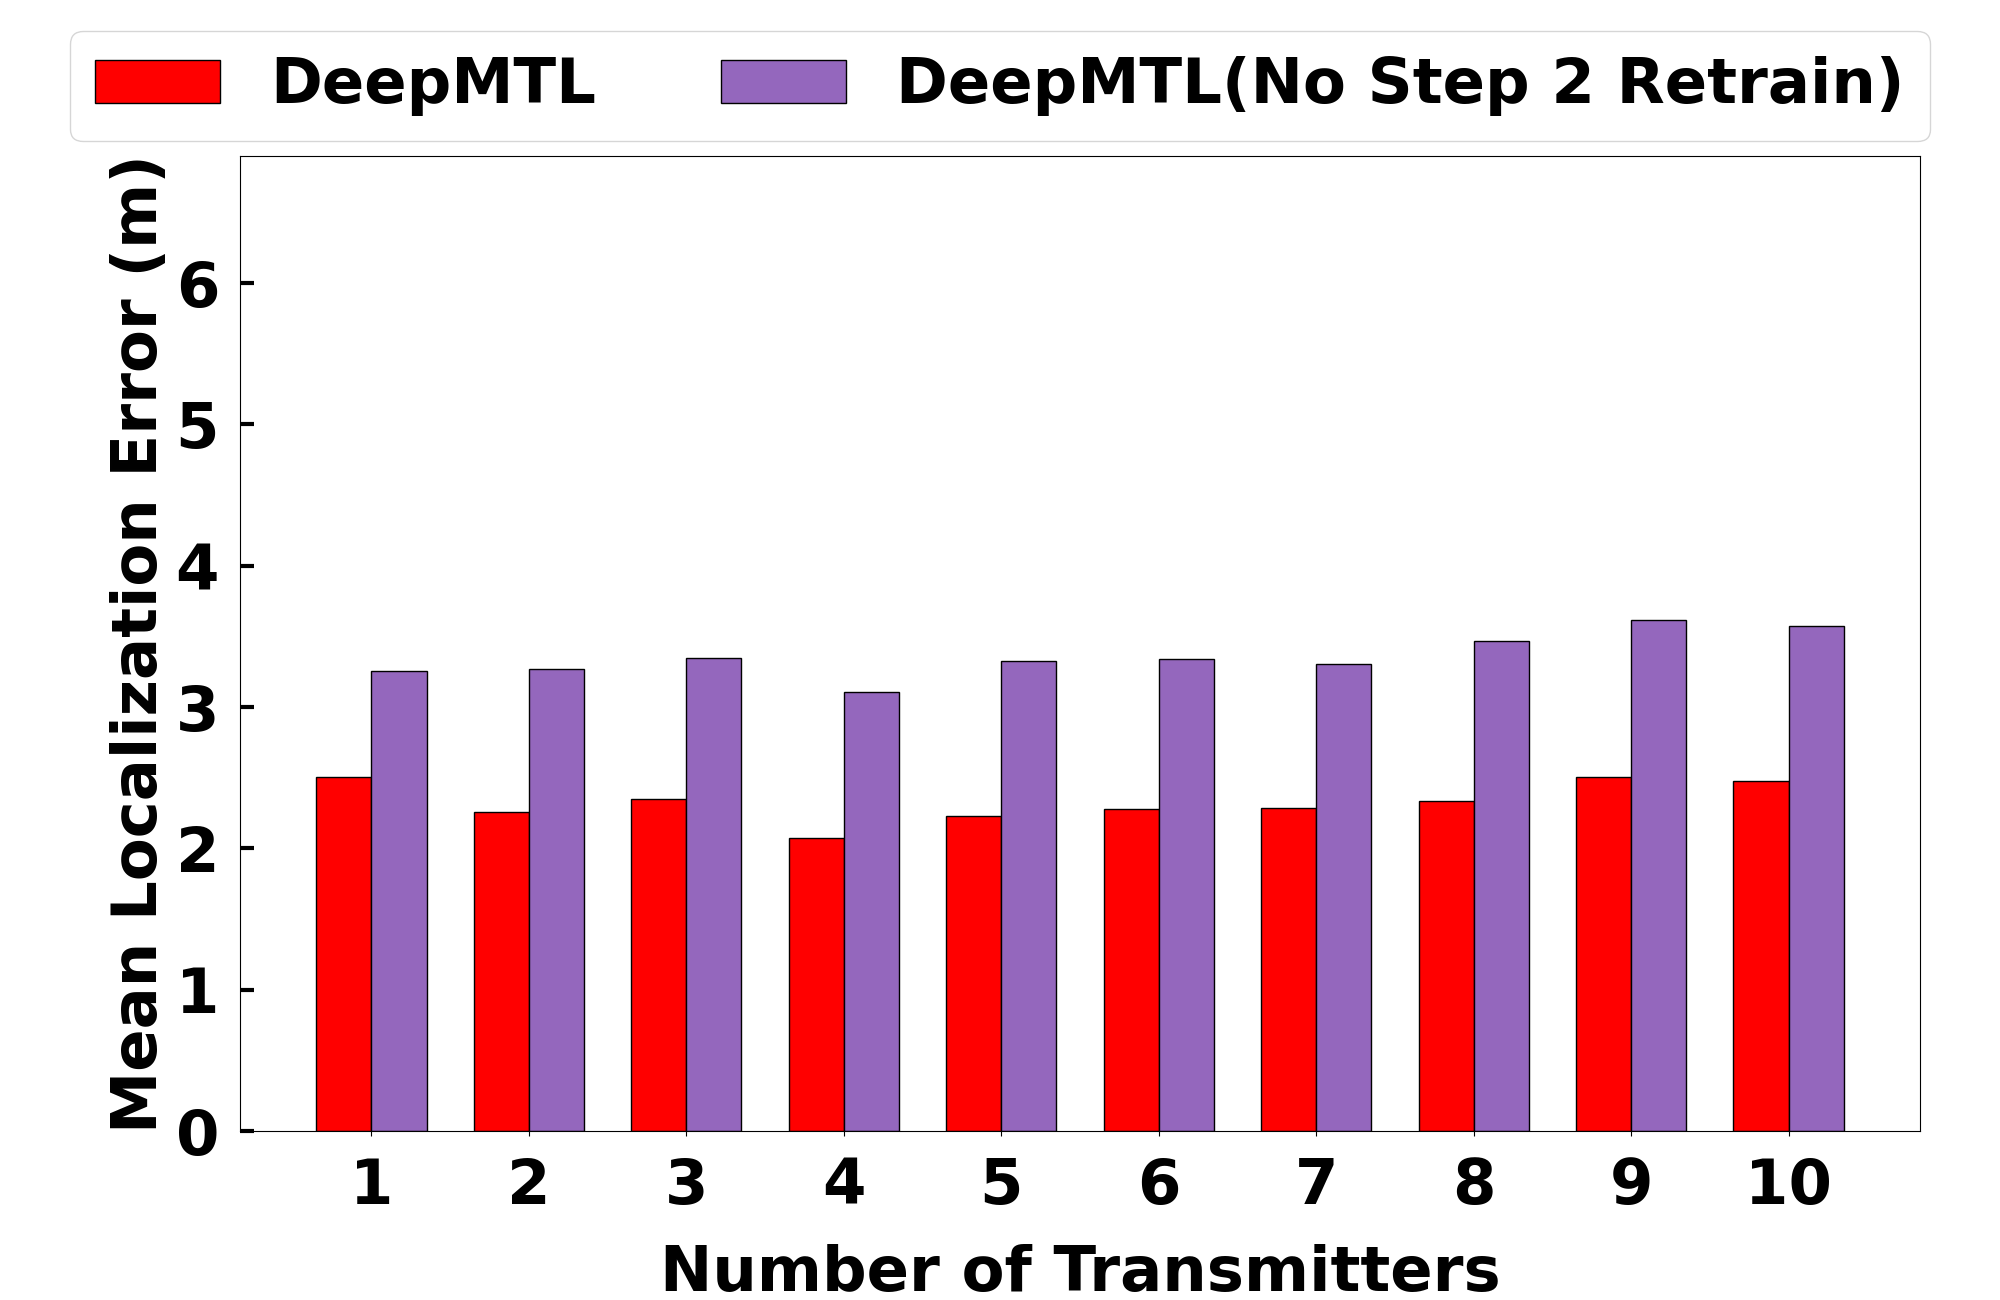
\includegraphics[width=\textwidth]{chapters/wowmom-pmc/figures/noretrain-logdistance-error-vary_numintru.png}
        \caption{First step trained in log-distance data, while the second step trained in SPLAT! data. Tested on the log-distance data.}
        \label{fig:notrain-logdist}
    \end{subfigure}%
    ~
    \begin{subfigure}[t]{0.48\textwidth}
        \centering
        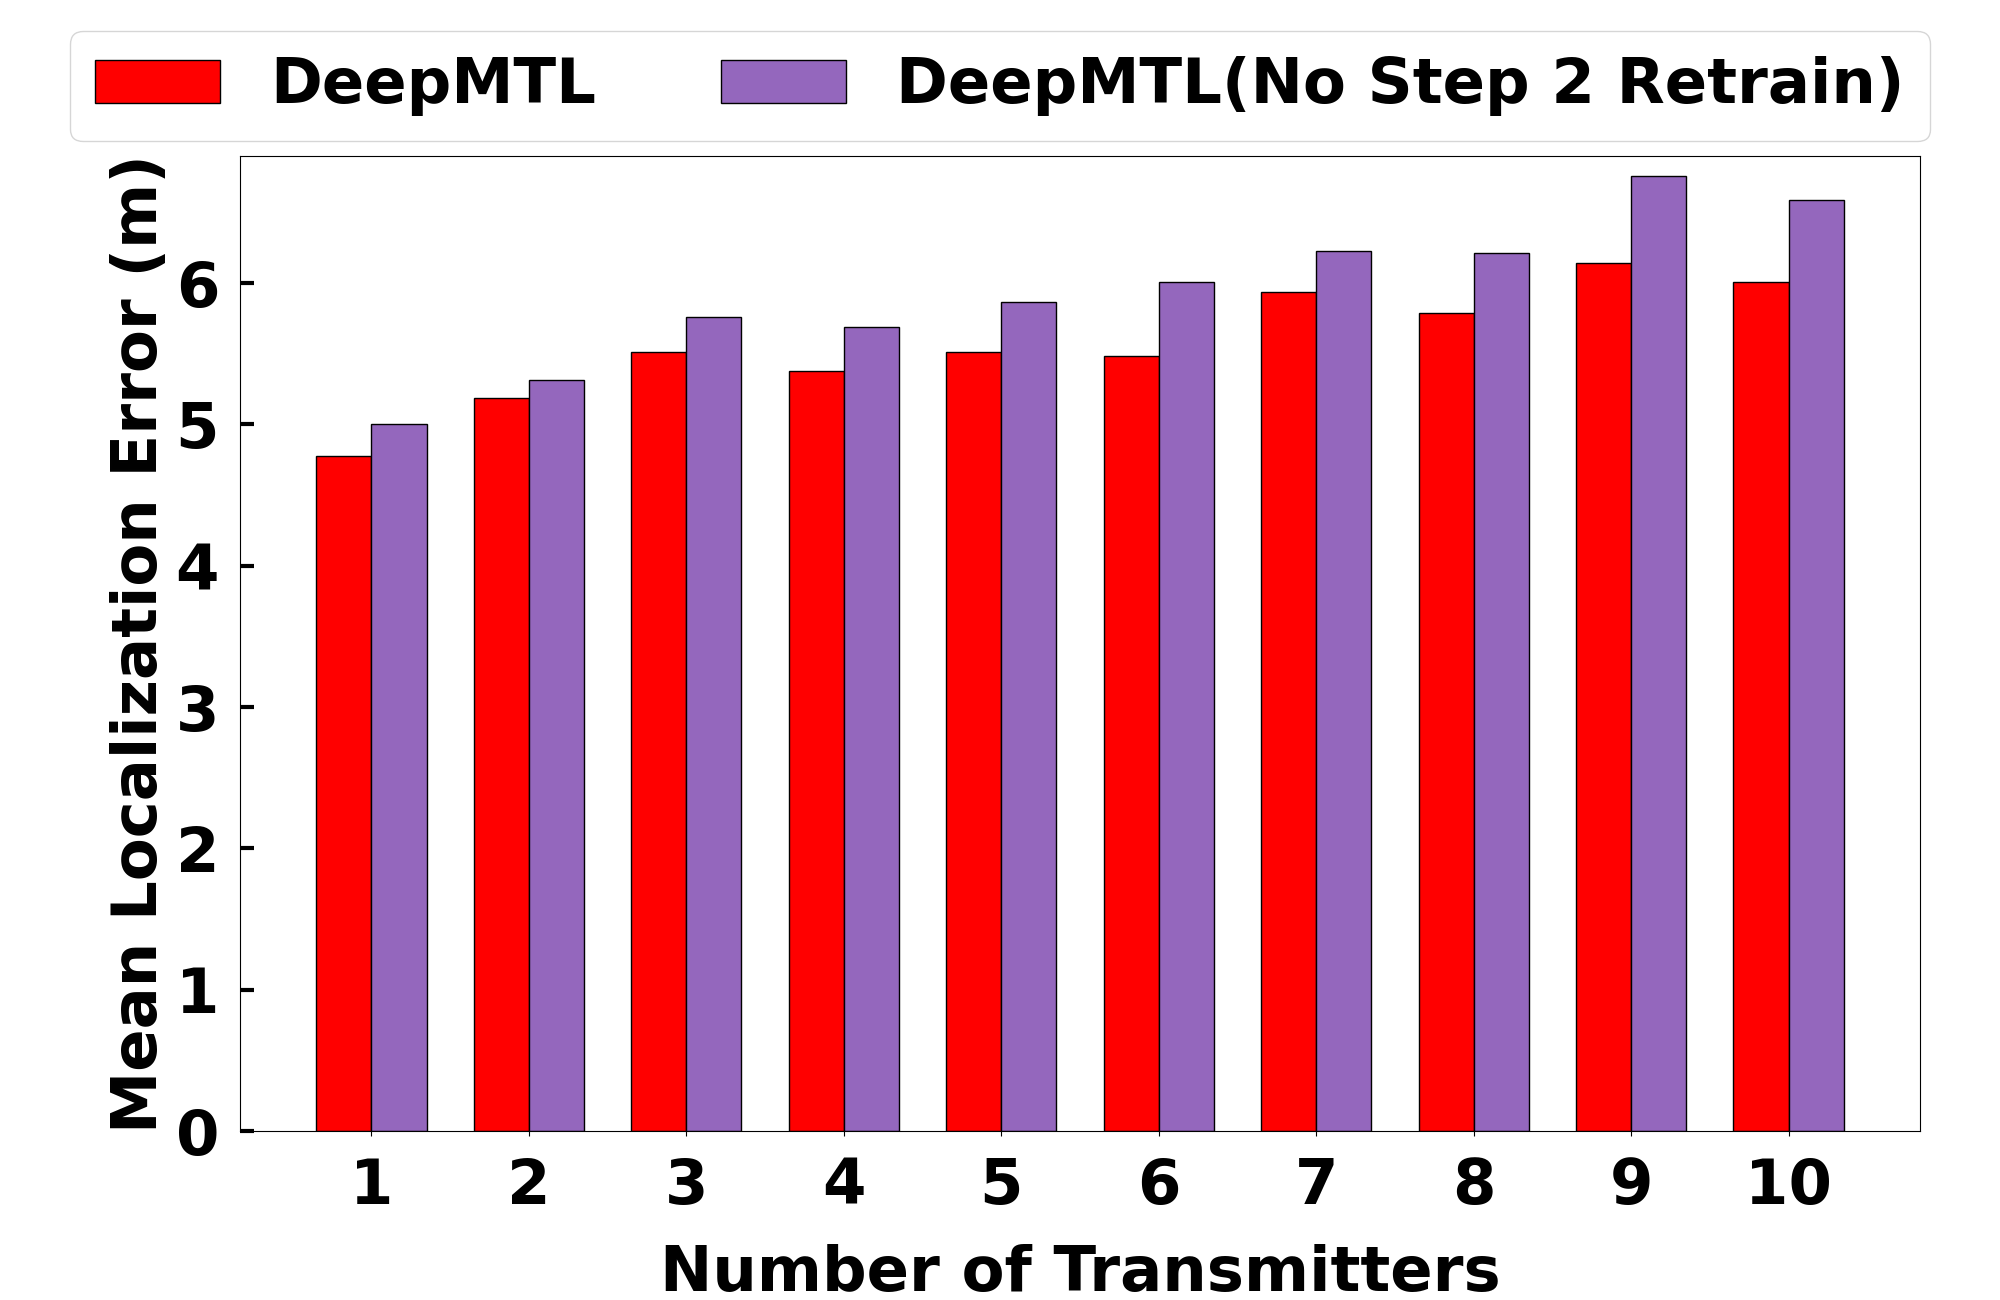
\includegraphics[width=\textwidth]{chapters/wowmom-pmc/figures/noretrain-splat-error-vary_numintru.png}
        \caption{First step trained in SPLAT! data, while second the step trained in log-distance data. Tested on the SPLAT! data.}
        \label{fig:notrain-splat}
    \end{subfigure}
    \caption{Localization error for varying number of transmitters when the first and second step of \our are trained on different training dataset.}
    \label{fig:notrain}
\end{figure*}

\begin{figure*}[t!]
    \centering
    \begin{subfigure}[t]{0.48\textwidth}
        \centering
        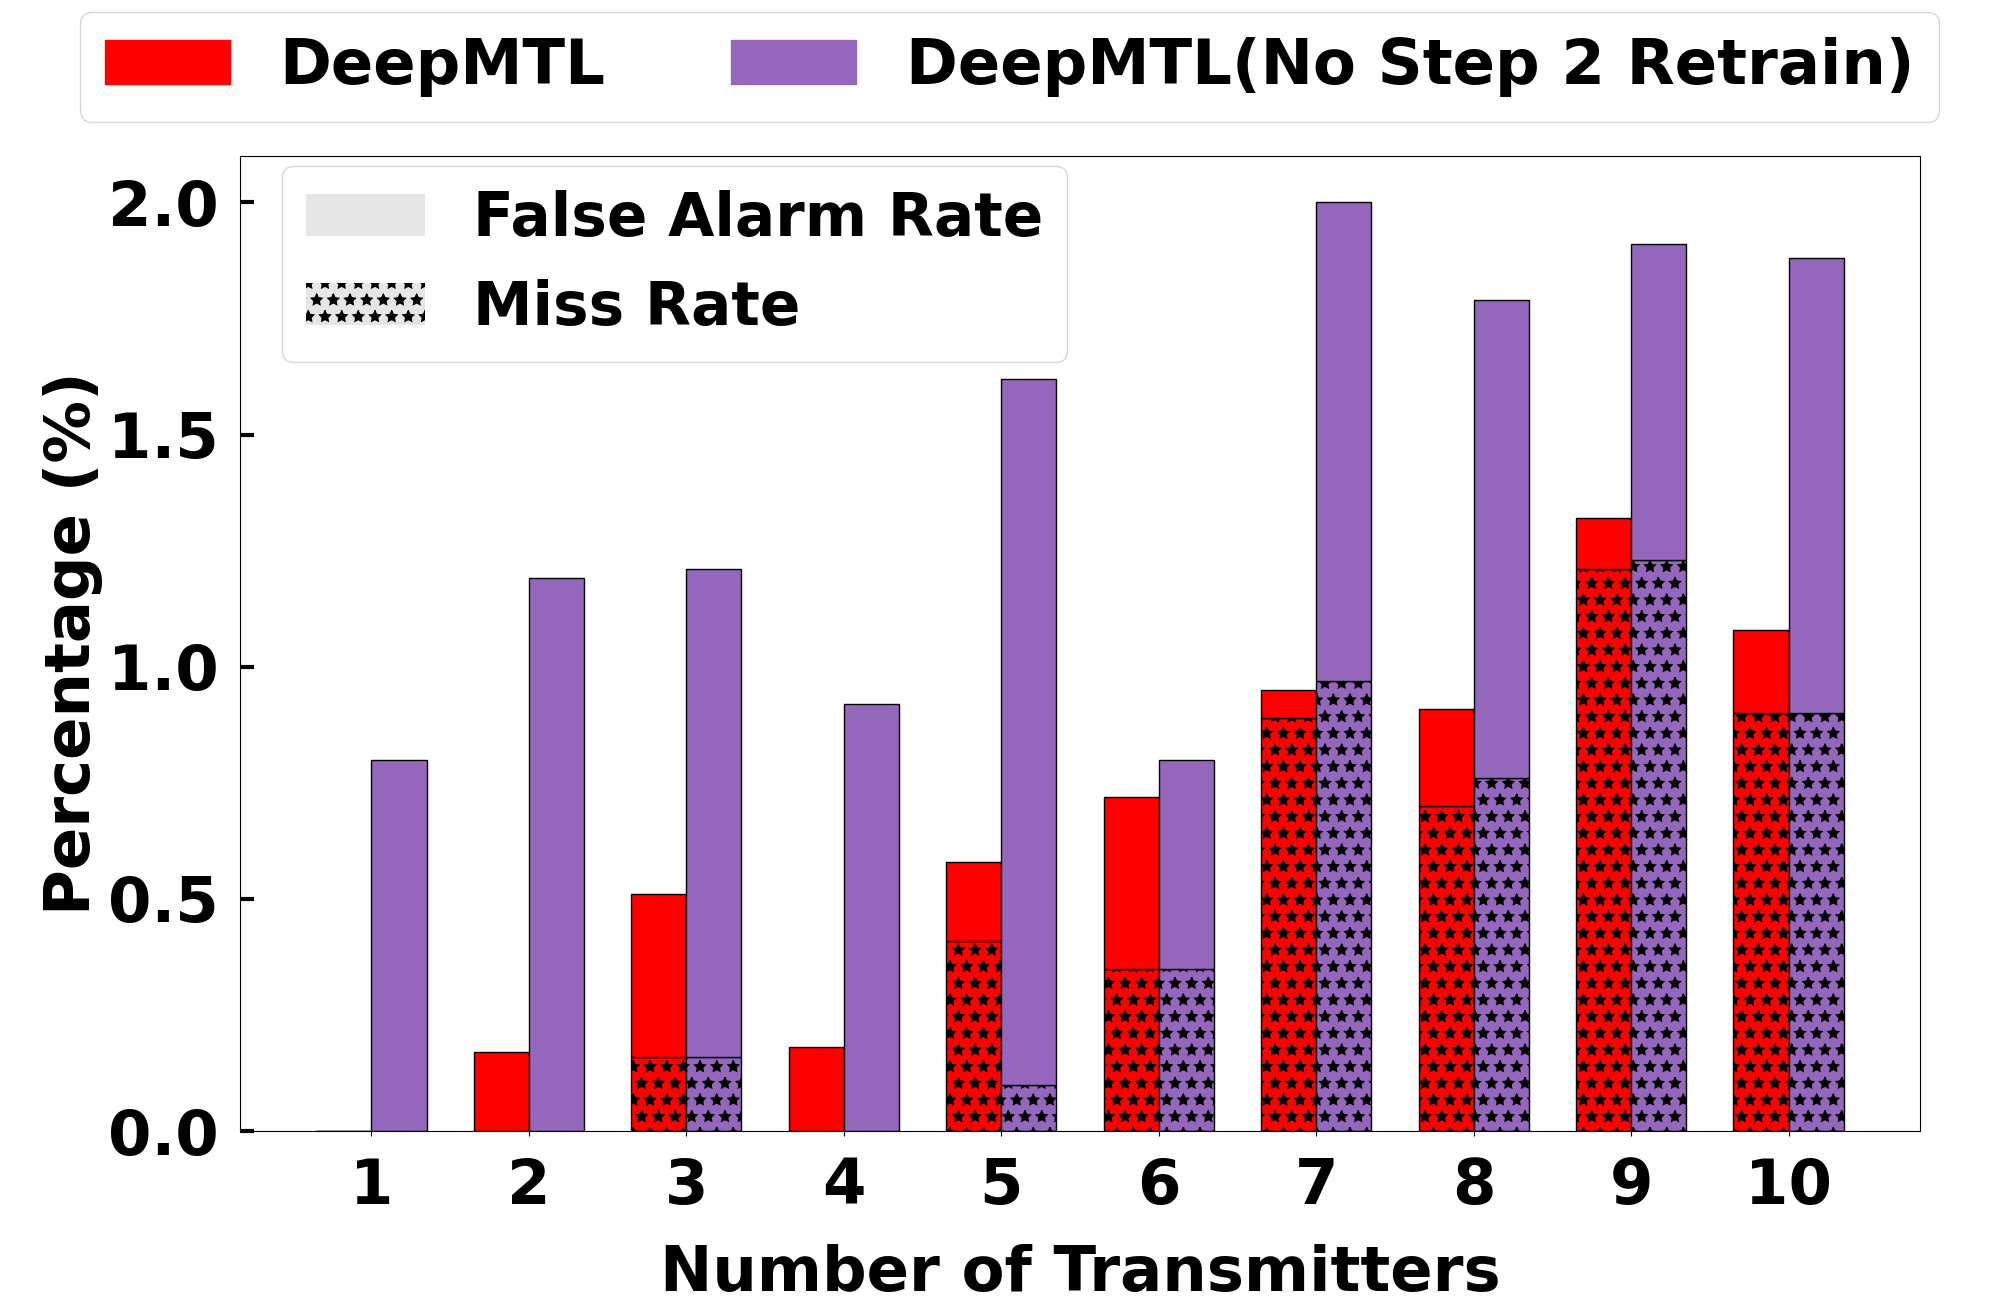
\includegraphics[width=\textwidth]{chapters/wowmom-pmc/figures/noretrain-logdistance-missfalse-vary_numintru.png}
        \caption{First step trained in log-distance data, while second step trained in SPLAT! data. Tested on the log-distance data.}
        \label{fig:notrain-logdist-missfalse}
    \end{subfigure}%
    ~ 
    \begin{subfigure}[t]{0.48\textwidth}
        \centering
        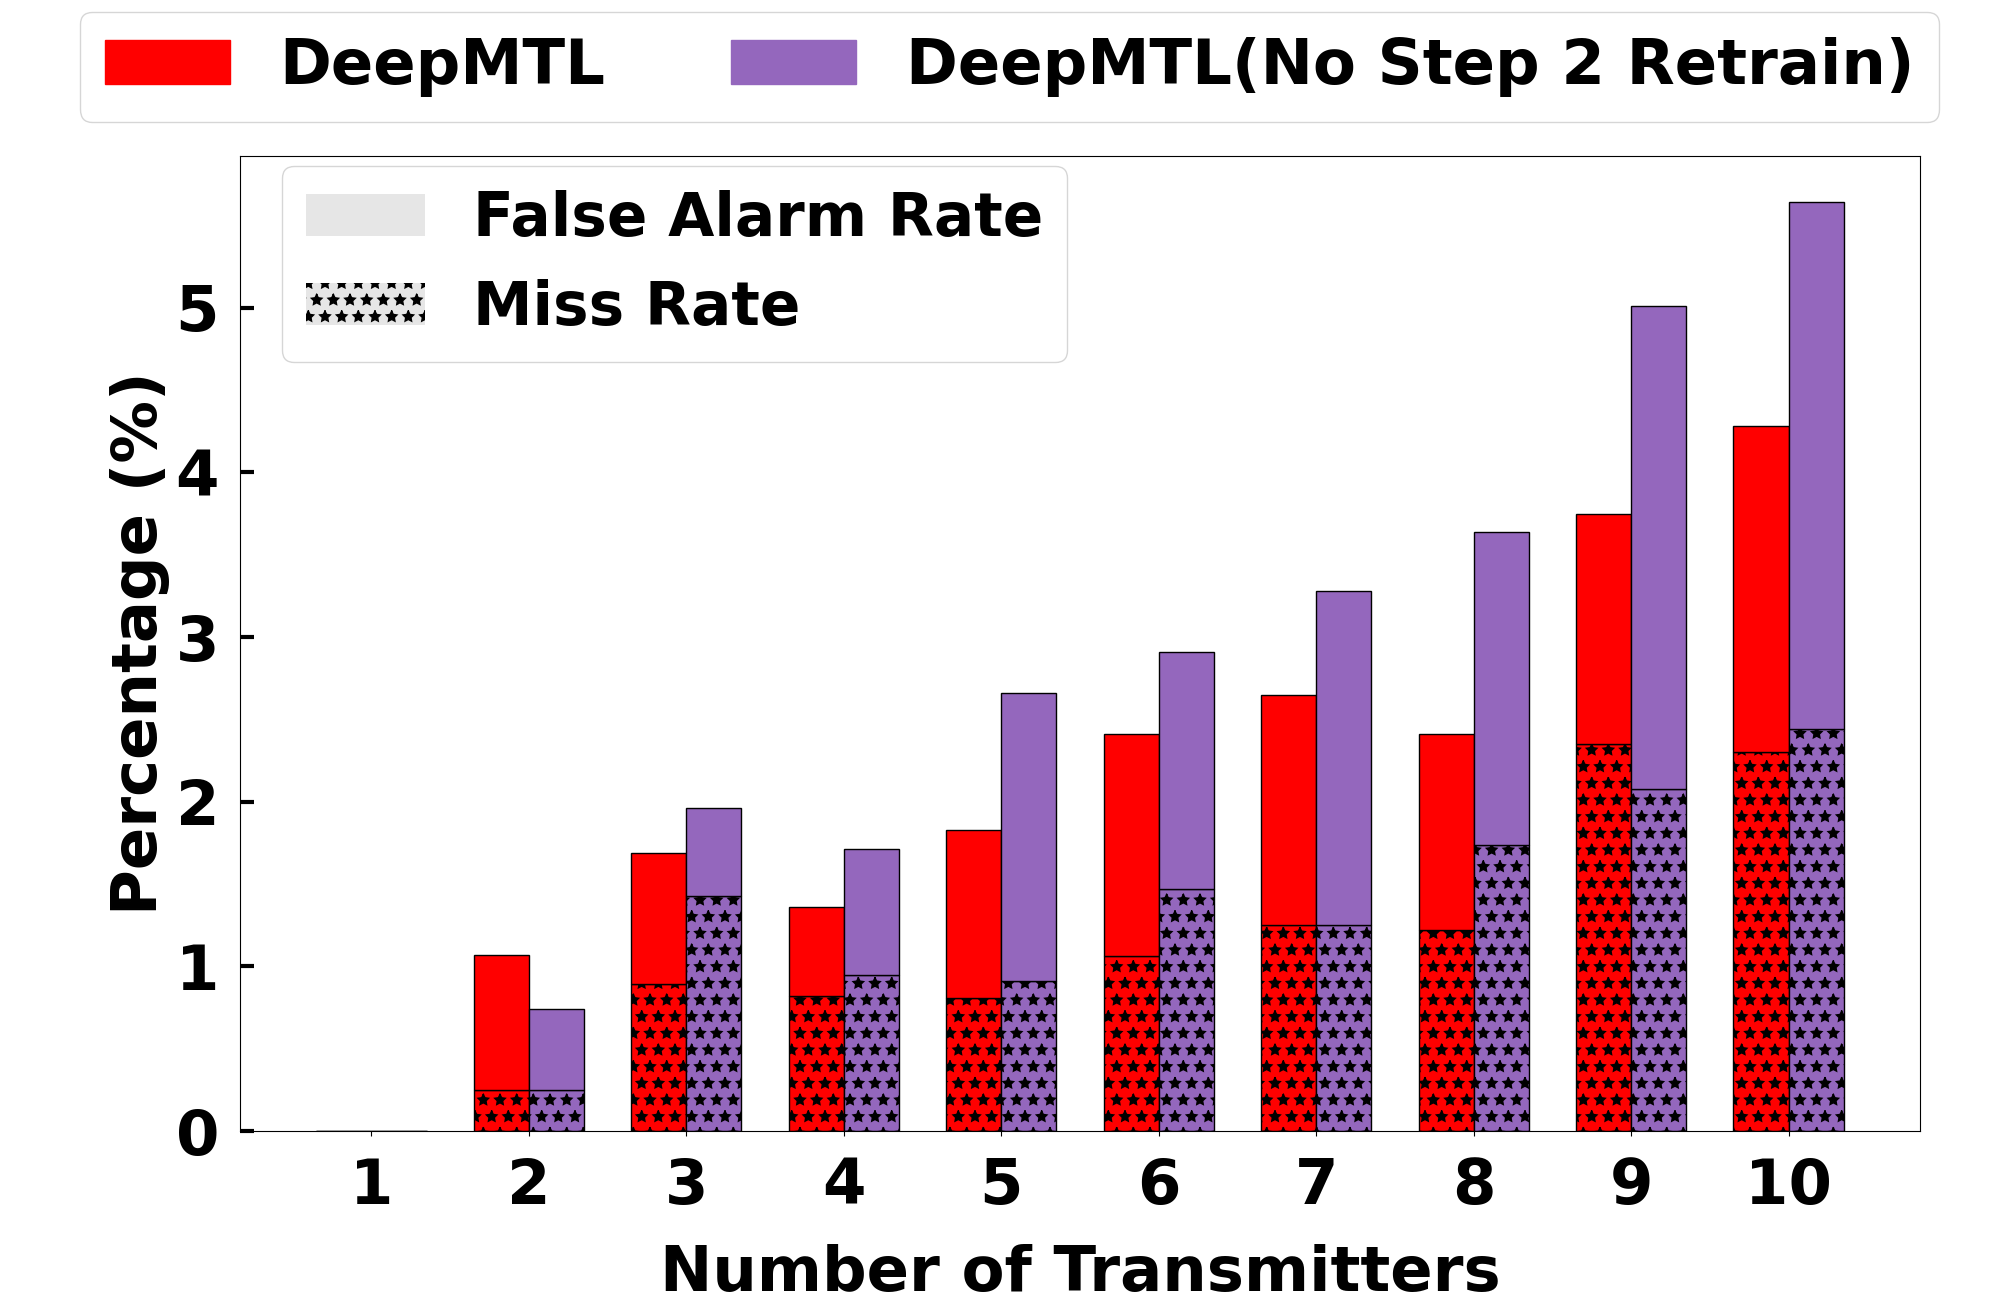
\includegraphics[width=\textwidth]{chapters/wowmom-pmc/figures/noretrain-splat-missfalse-vary_numintru.png}
        \caption{First step trained in SPLAT! data, while second step trained in log-distance! data. Tested on the SPLAT! data.}
        \label{fig:notrain-splat-missfalse}
    \end{subfigure}
    \caption{The miss rate and false alarm rate for varying number of transmitters when the first and second step of \our are trained on different training dataset.}
    \label{fig:notrain-missfalse}
\end{figure*}

We demonstrate transfer learning (generalizability) by showing that the second step in \our does not need to be retrained for different radio frequency propagation models and terrains.
In the previous experiments, the two steps of \our are both trained in the same setting, either log-distance or SPLAT!.
We do the following two combinations to show that the second step does not need to retrain:
\begin{enumerate}
    \item The first step is trained in the log-distance setting and the second step is trained in the SPLAT! setting. Tested on the log-distance data.
    \item The first step is trained in the SPLAT! setting and the second step is trained in the log-distance setting. Tested on the SPLAT! data.
\end{enumerate}
In both combinations, the second step \yolocust is trained on a different dataset compared to the first step \imgimg. 
Fig.~\ref{fig:notrain-logdist} shows that the localization error increases one-third in the first combination compared to the case where both the first and second steps are trained on log-distance dataset. 
Fig.~\ref{fig:notrain-splat} shows that the localization error increases only five percent in the second combination compared to the case where both the first and second steps are trained on SPLAT! dataset.
The miss rate and false alarm rate for both combinations also increase minimally, i.e. the summation of miss rate and false alarm rate only increases around 1\% in absolute value. See Fig.~\ref{fig:notrain-missfalse}.
This implies that the second step of \our, \yolocust, is general and does not need to retrain for different radio frequency propagation models and terrains.
This is because the first step \imgimg is translating sensor readings images from different geographical areas to the same Gaussian peaks.
The first step \imgimg still needs to be retrained for different situations to translate the sensor readings to the peaks.


\subsection{Localize Intruders in the Presence of Authorized Users}
\label{subsec:authorzedeval}

The previous experiment setting is based on the assumption that all transmitters we are localizing are intruders.
Different than the previous setting, here, we put five authorized users and they are spread out in the field, so those five will not interfere with each other.
This is the more general version of the \mtl problem, where there are some authorized users in the background.
Fig.~\ref{fig:authorized_error} shows the localization error of two approaches localizing intruders in the presence of five authorized users with a varying number of intruders.
It is observed that the first approach, localize then remove authorized users, has a ten to twenty percent smaller localization error compared to the second approach, subtract authorized user power then localize.
This is due to the inaccuracy of power subtraction from the \subtract.
Fig.~\ref{fig:authorized_missfalse} shows the miss and false alarm of two approaches localizing intruders in the presence of five authorized users with a varying number of intruders.
It is observed that the second approach, subtract authorized TX power then localize, is having a high false alarm when the number of intruders is three or less.
So for \subtract, subtracting the power of five background authorized users from six transmitters (five out of six transmitters are authorized users, one intruder) is relatively more difficult than subtracting the power of five authorized users from nine users (five out of nine transmitters are authorized users, four intruders). 
Also statistically, getting one false alarm when there are one intruder and five authorized users is 100\% false alarm rate, while getting one false alarm when there are two intruders and five authorized users is only 50\% false alarm rate (the denominator is the number of intruders).
Thus, the false alarm rate for one and two number of intruders looks to differ a lot, but in reality, the false alarm cases do not differ a lot).
When the number of intruders is three or four, the two approaches are comparable. But when the number of intruders is larger than four, the second approach is having a lower miss and false alarm rate.
In summary, the two approaches both have their strengths.
The main advantage for the second approach is that the sum of miss rate and false alarm rate is lower when the number of intruders is large.

\begin{figure}[t]
    \centering
    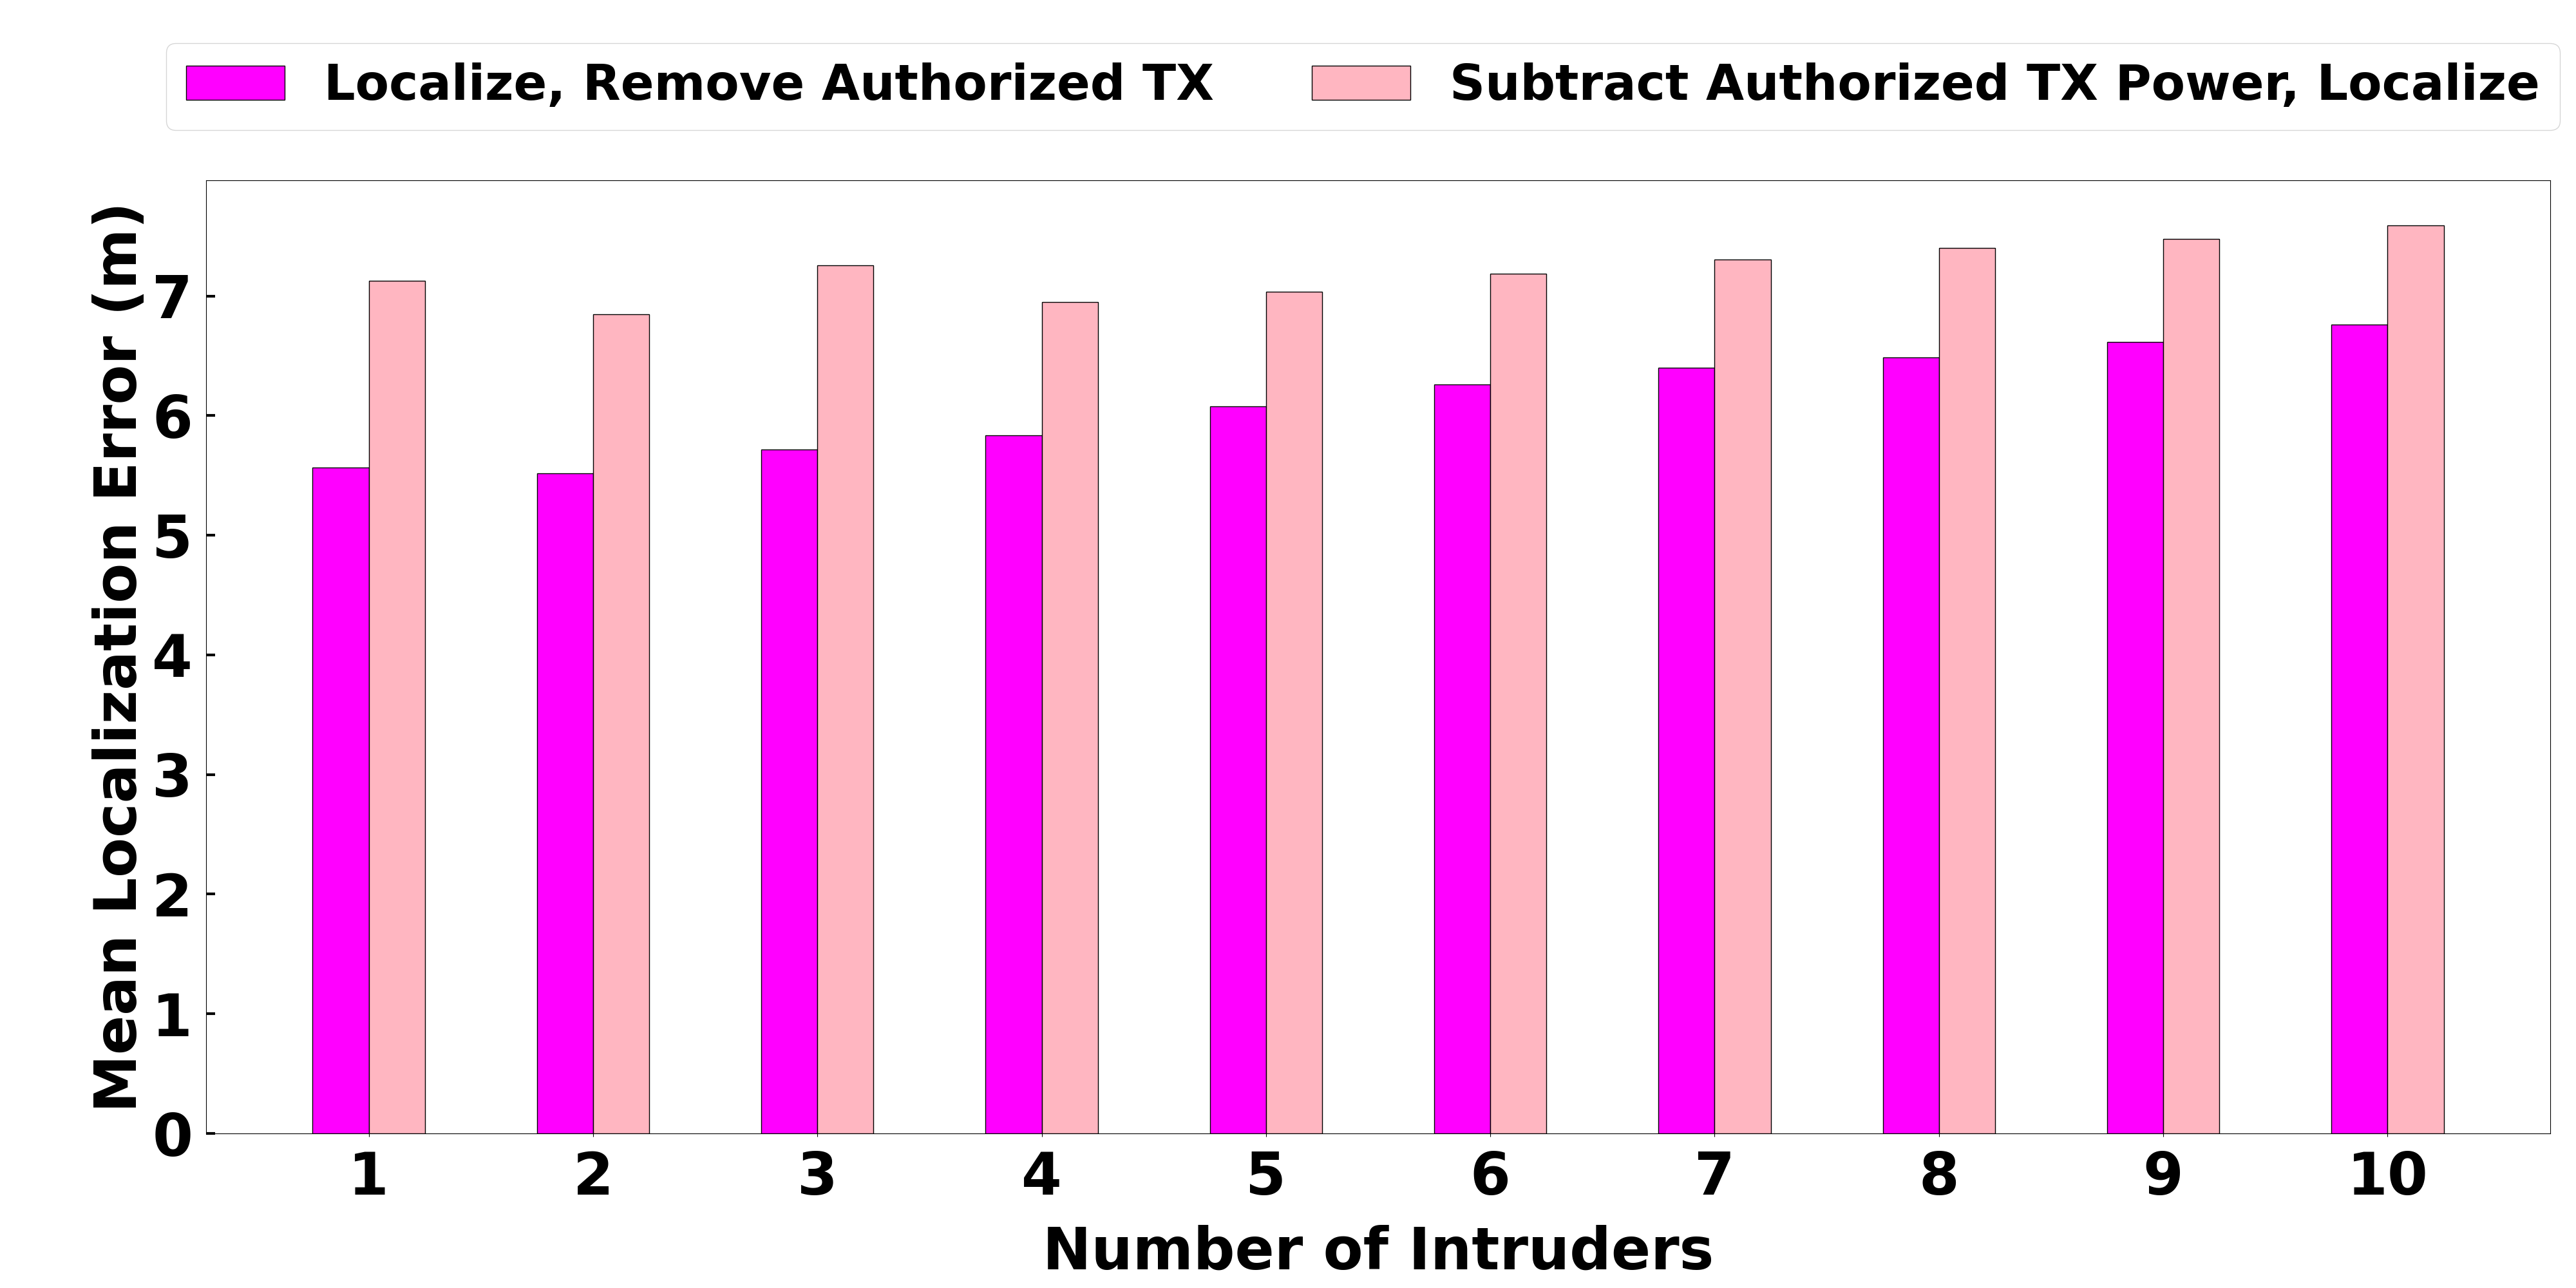
\includegraphics[width=0.75\textwidth]{chapters/wowmom-pmc/figures/splat-error-authorized-varyintru.png}
    \caption{The localization error of two approaches in the presence of five authorized users with varying number of intruders.}
    \label{fig:authorized_error}
\end{figure}

\begin{figure}[t]
    \centering
    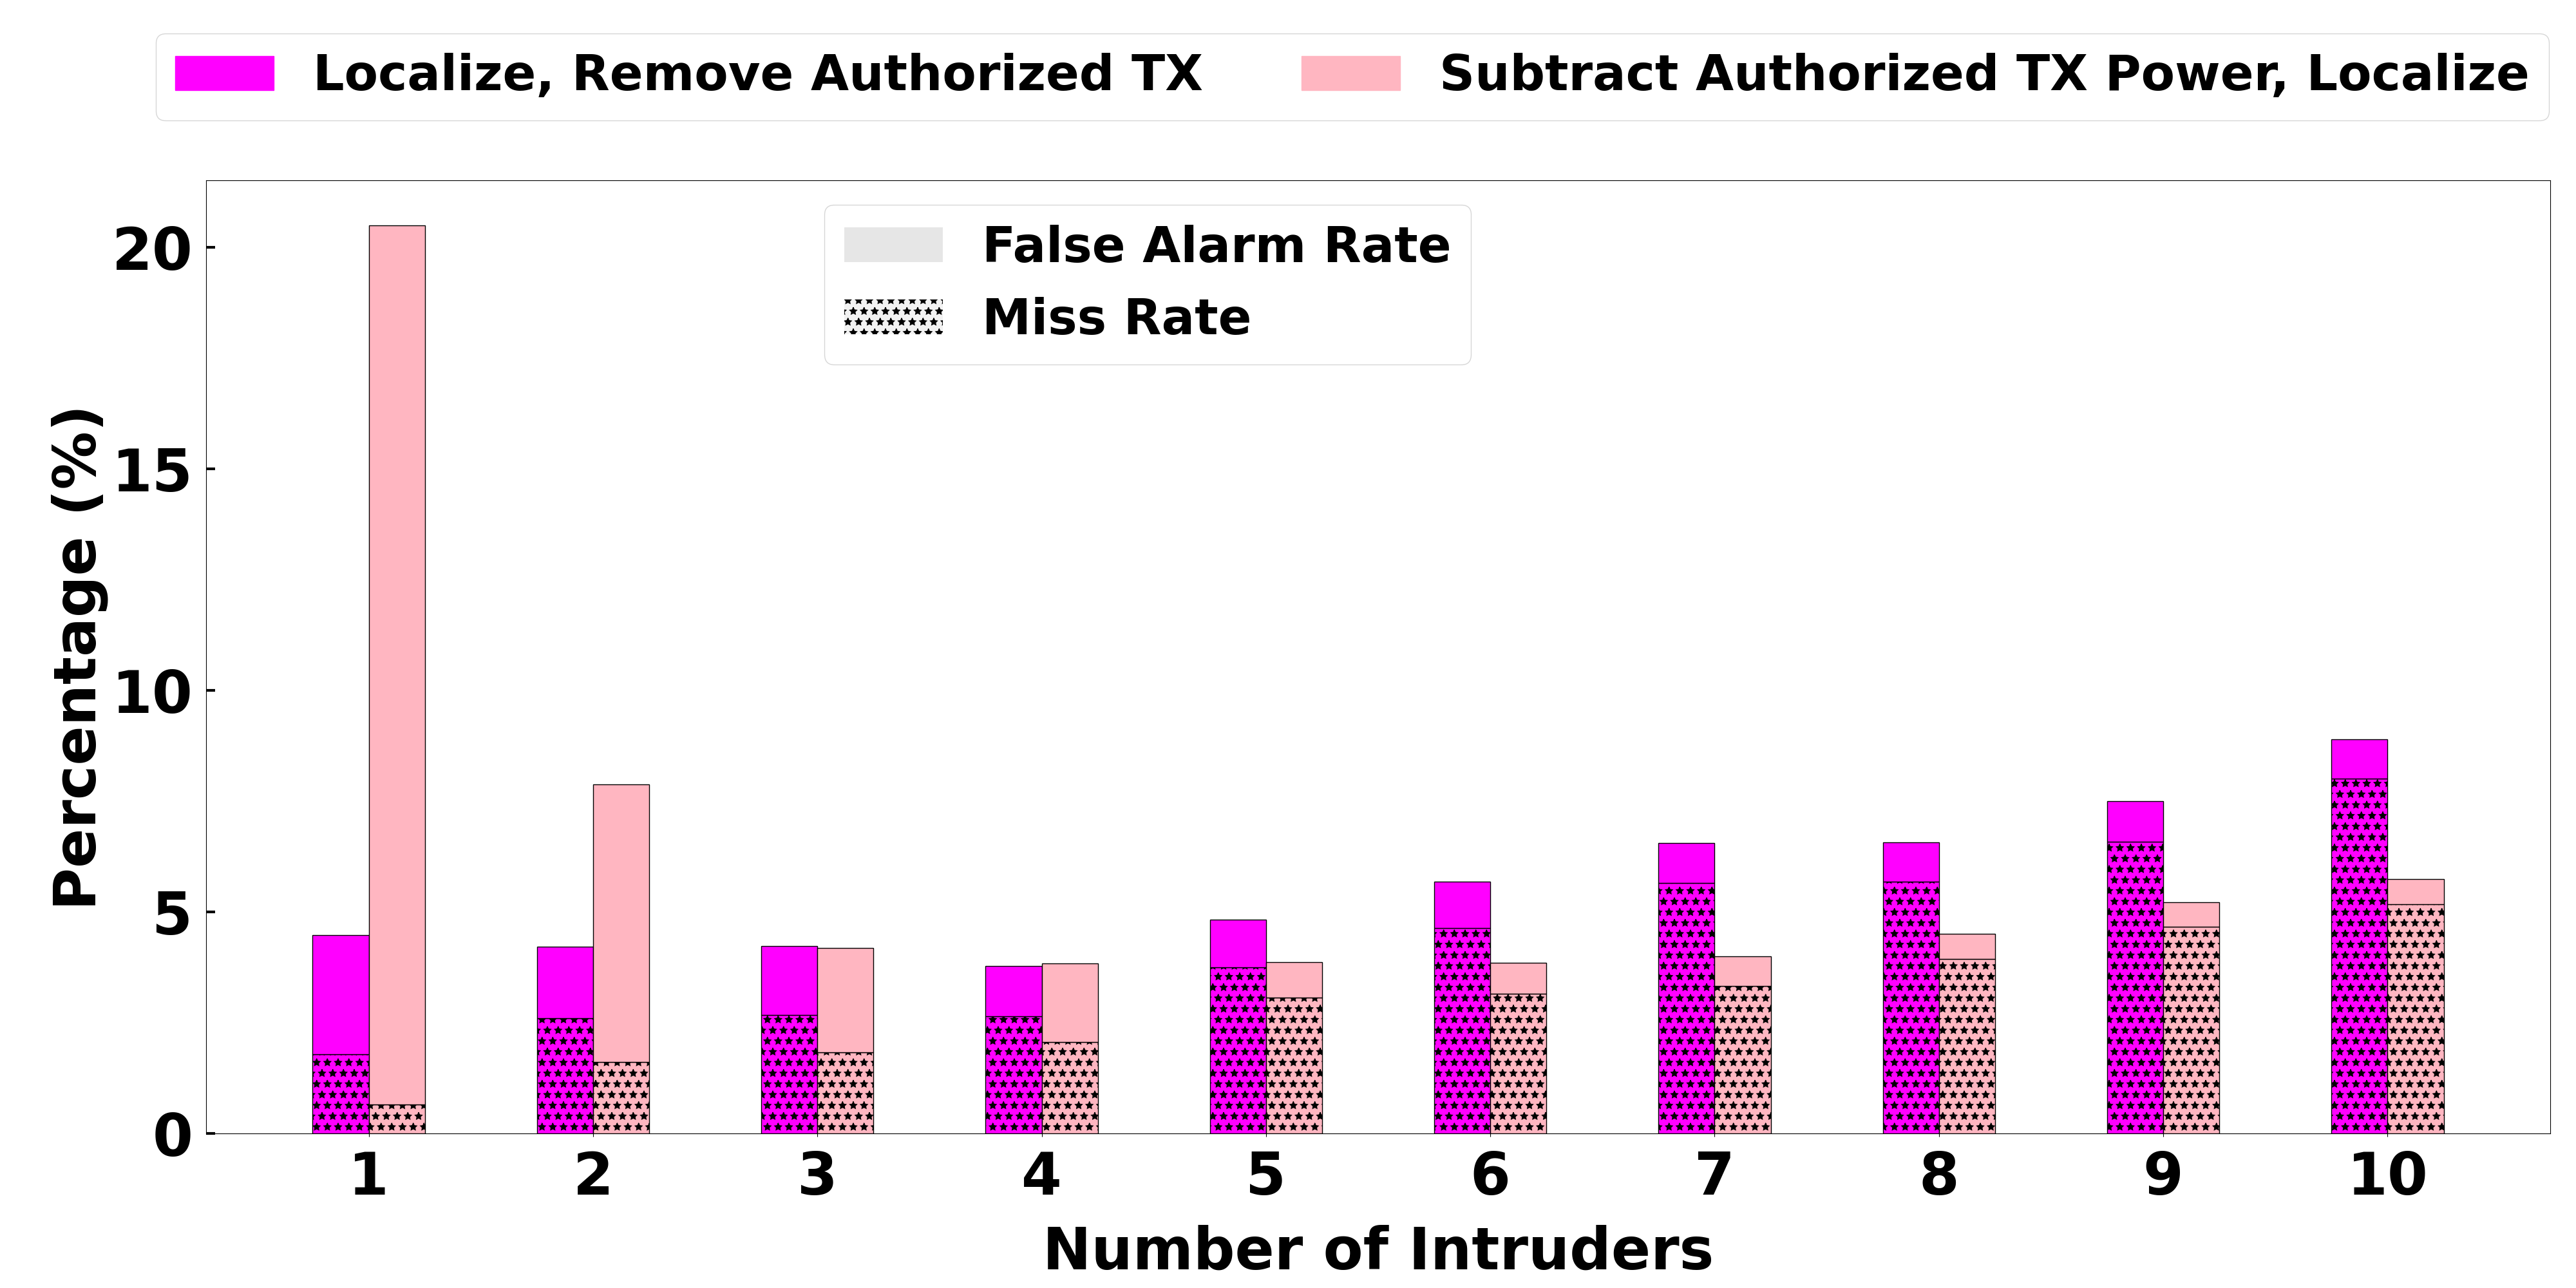
\includegraphics[width=0.75\textwidth]{chapters/wowmom-pmc/figures/splat-missfalse-authorized-varyintru.png}
    \caption{The miss and false alarm of two localization approaches in the presence of 5 authorized users with varying number of intruders.}
    \label{fig:authorized_missfalse}
\end{figure}




\subsection{Power Estimation Evaluation}
\label{subsec:powereval}
In this subsection, we evaluate the transmitter power estimation performance.
In all experiments, the power range is 5 dB.
The power error is presented in absolute value.
A power error of 0.5 dB implies a relative power error of 10\%.
First, we compare the single transmitter power estimation between \map and \power, and then compare the multiple transmitter power estimation between \map, \power with error correction, and \power with error correction.

\begin{figure}
    \centering
    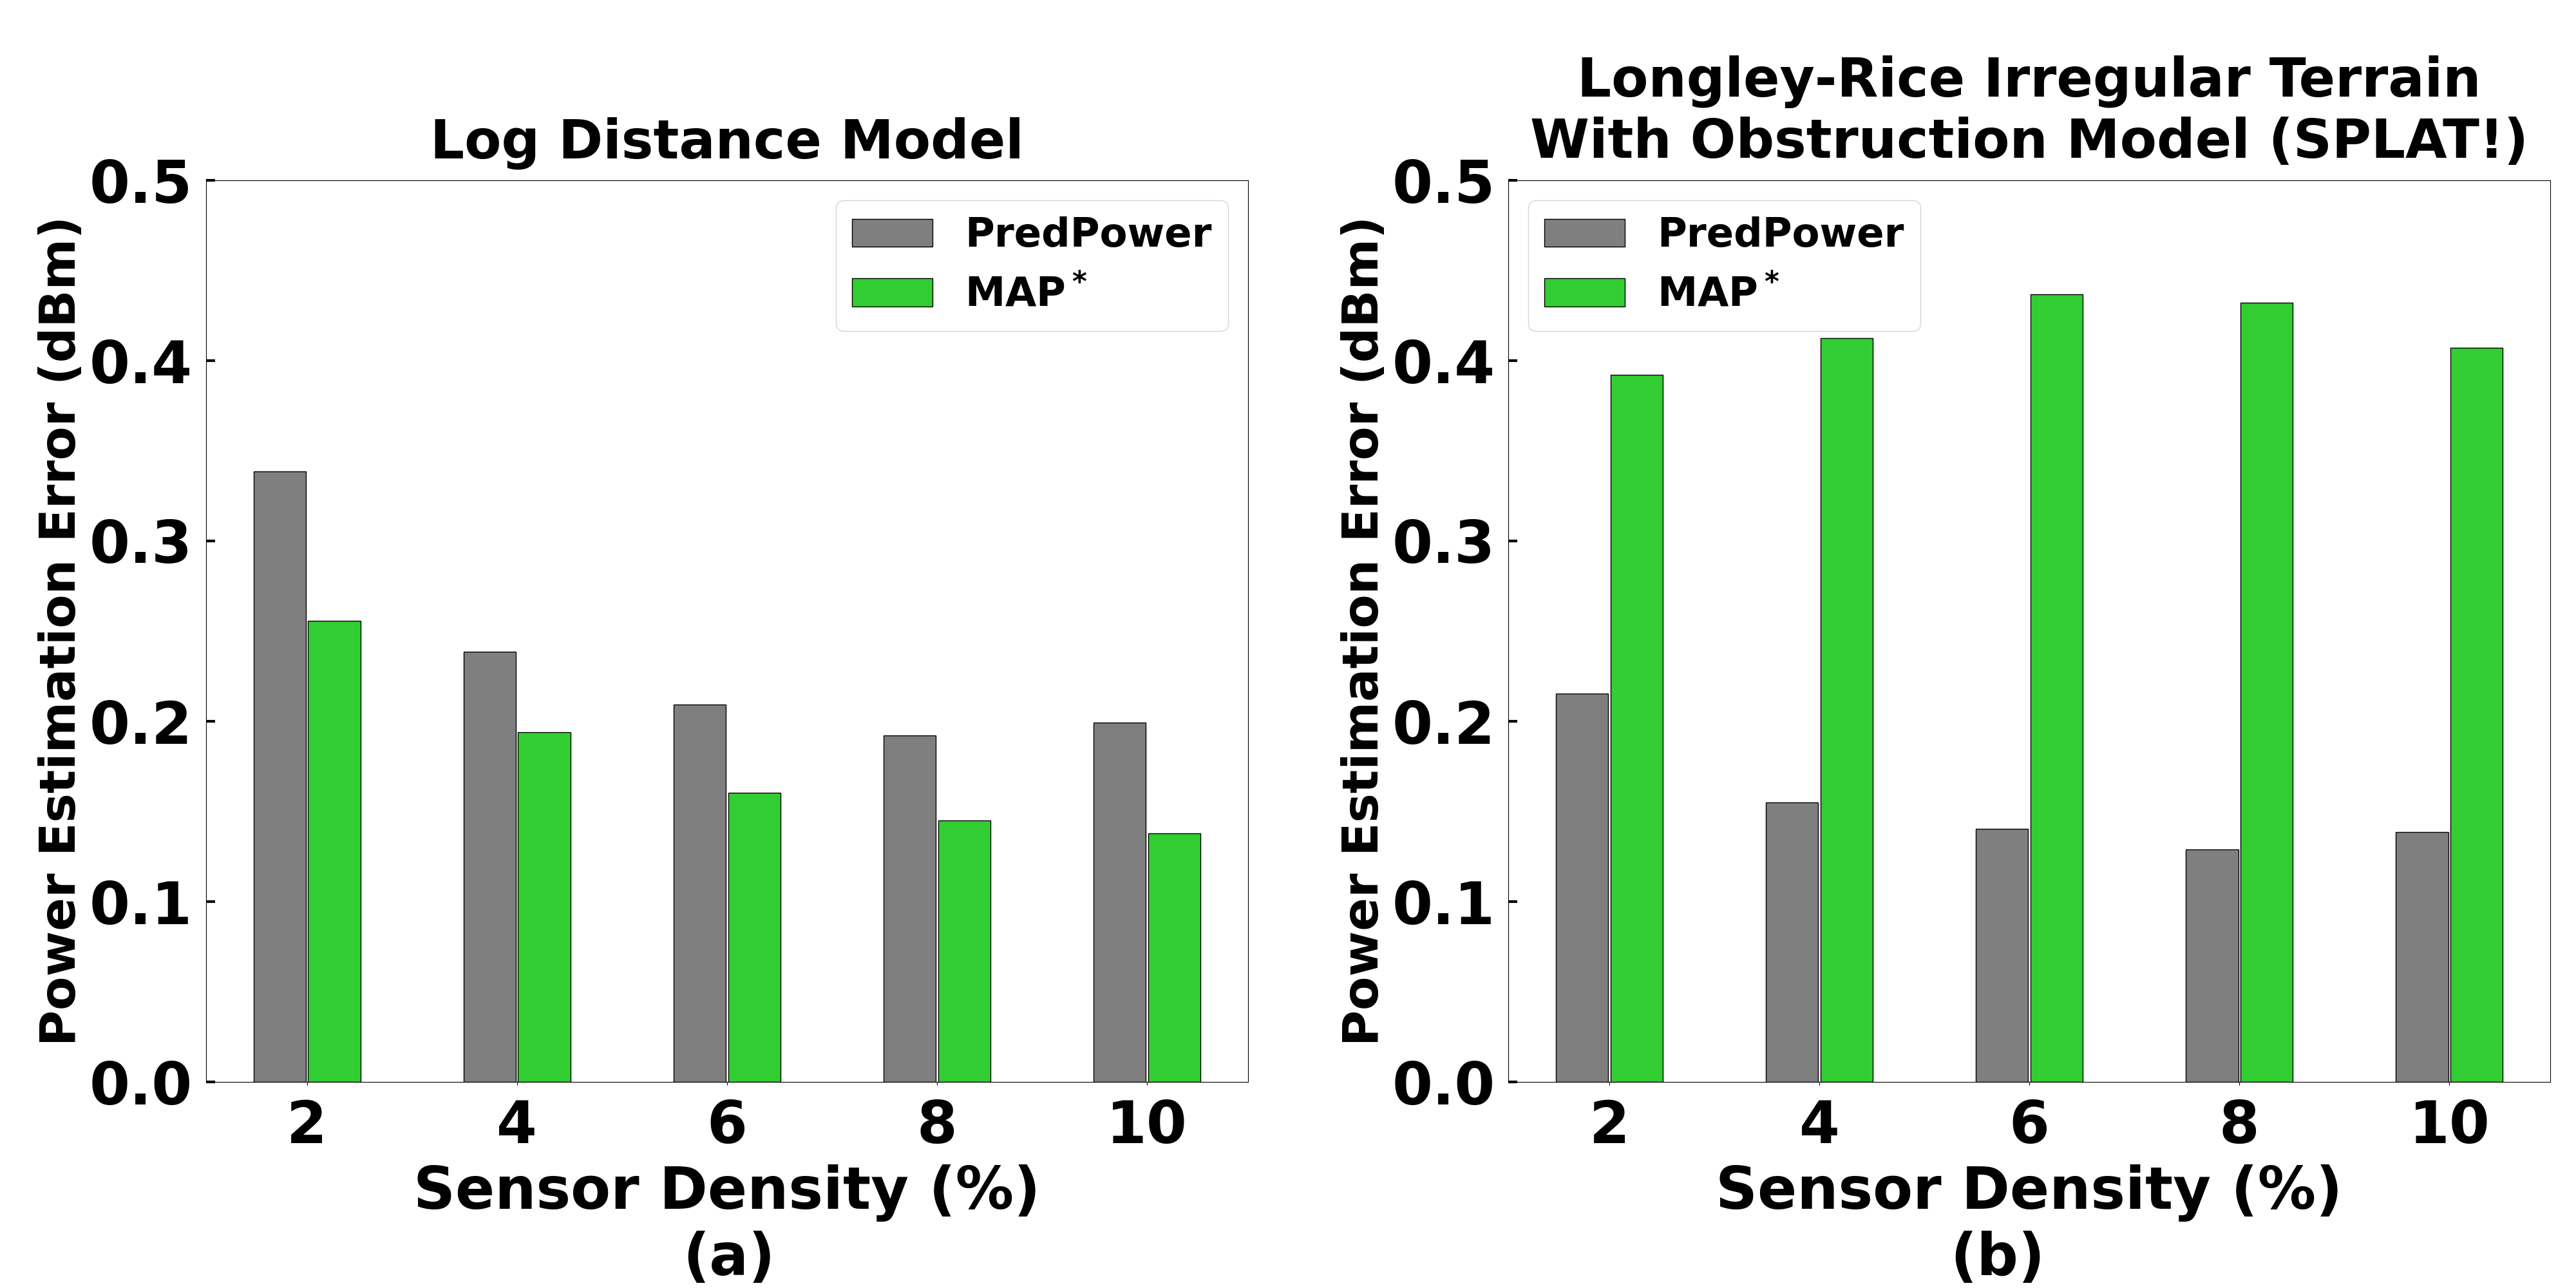
\includegraphics[width=0.75\textwidth]{chapters/wowmom-pmc/figures/powererror_varysensor.png}
    \caption{The single transmitter power estimation error of \power and \map in two propagation models, (a) Log-distance model and (b) Longley--Rice Irregular Terrain with Obstruction Model (SPLAT!), for varying sensor densities.}
    \label{fig:singleTXpower}
\end{figure}

Figure~\ref{fig:singleTXpower}(a) shows the performance of single transmitter power estimation in the log-distance propagation model scenario with varying sensor density.
In this case, \map has a 10 to 20 percent smaller power estimation error.
Figure~\ref{fig:singleTXpower}(b) shows the performance of single transmitter power estimation in the SPLAT! model with varying sensor density.
In this case, \power is significantly lower in power error.
So in average, \power outperforms \map in single transmitter power estimation.
We can also conclude that for \power, a higher sensor density will decrease the power estimation error. \
While a 2\% of sensor density will lead to a higher error, a sensor density of 6\% is enough to give relatively good results.

For multiple transmitter power estimation, we compare three methods in two propagation models and show that \power with error correction has the best performance among the three methods.
\power without error correction is expected to perform the worst and it suggests that the post-processing error correction stage for \power is important and works well.
%%%
\begin{figure}[t]
    \centering
    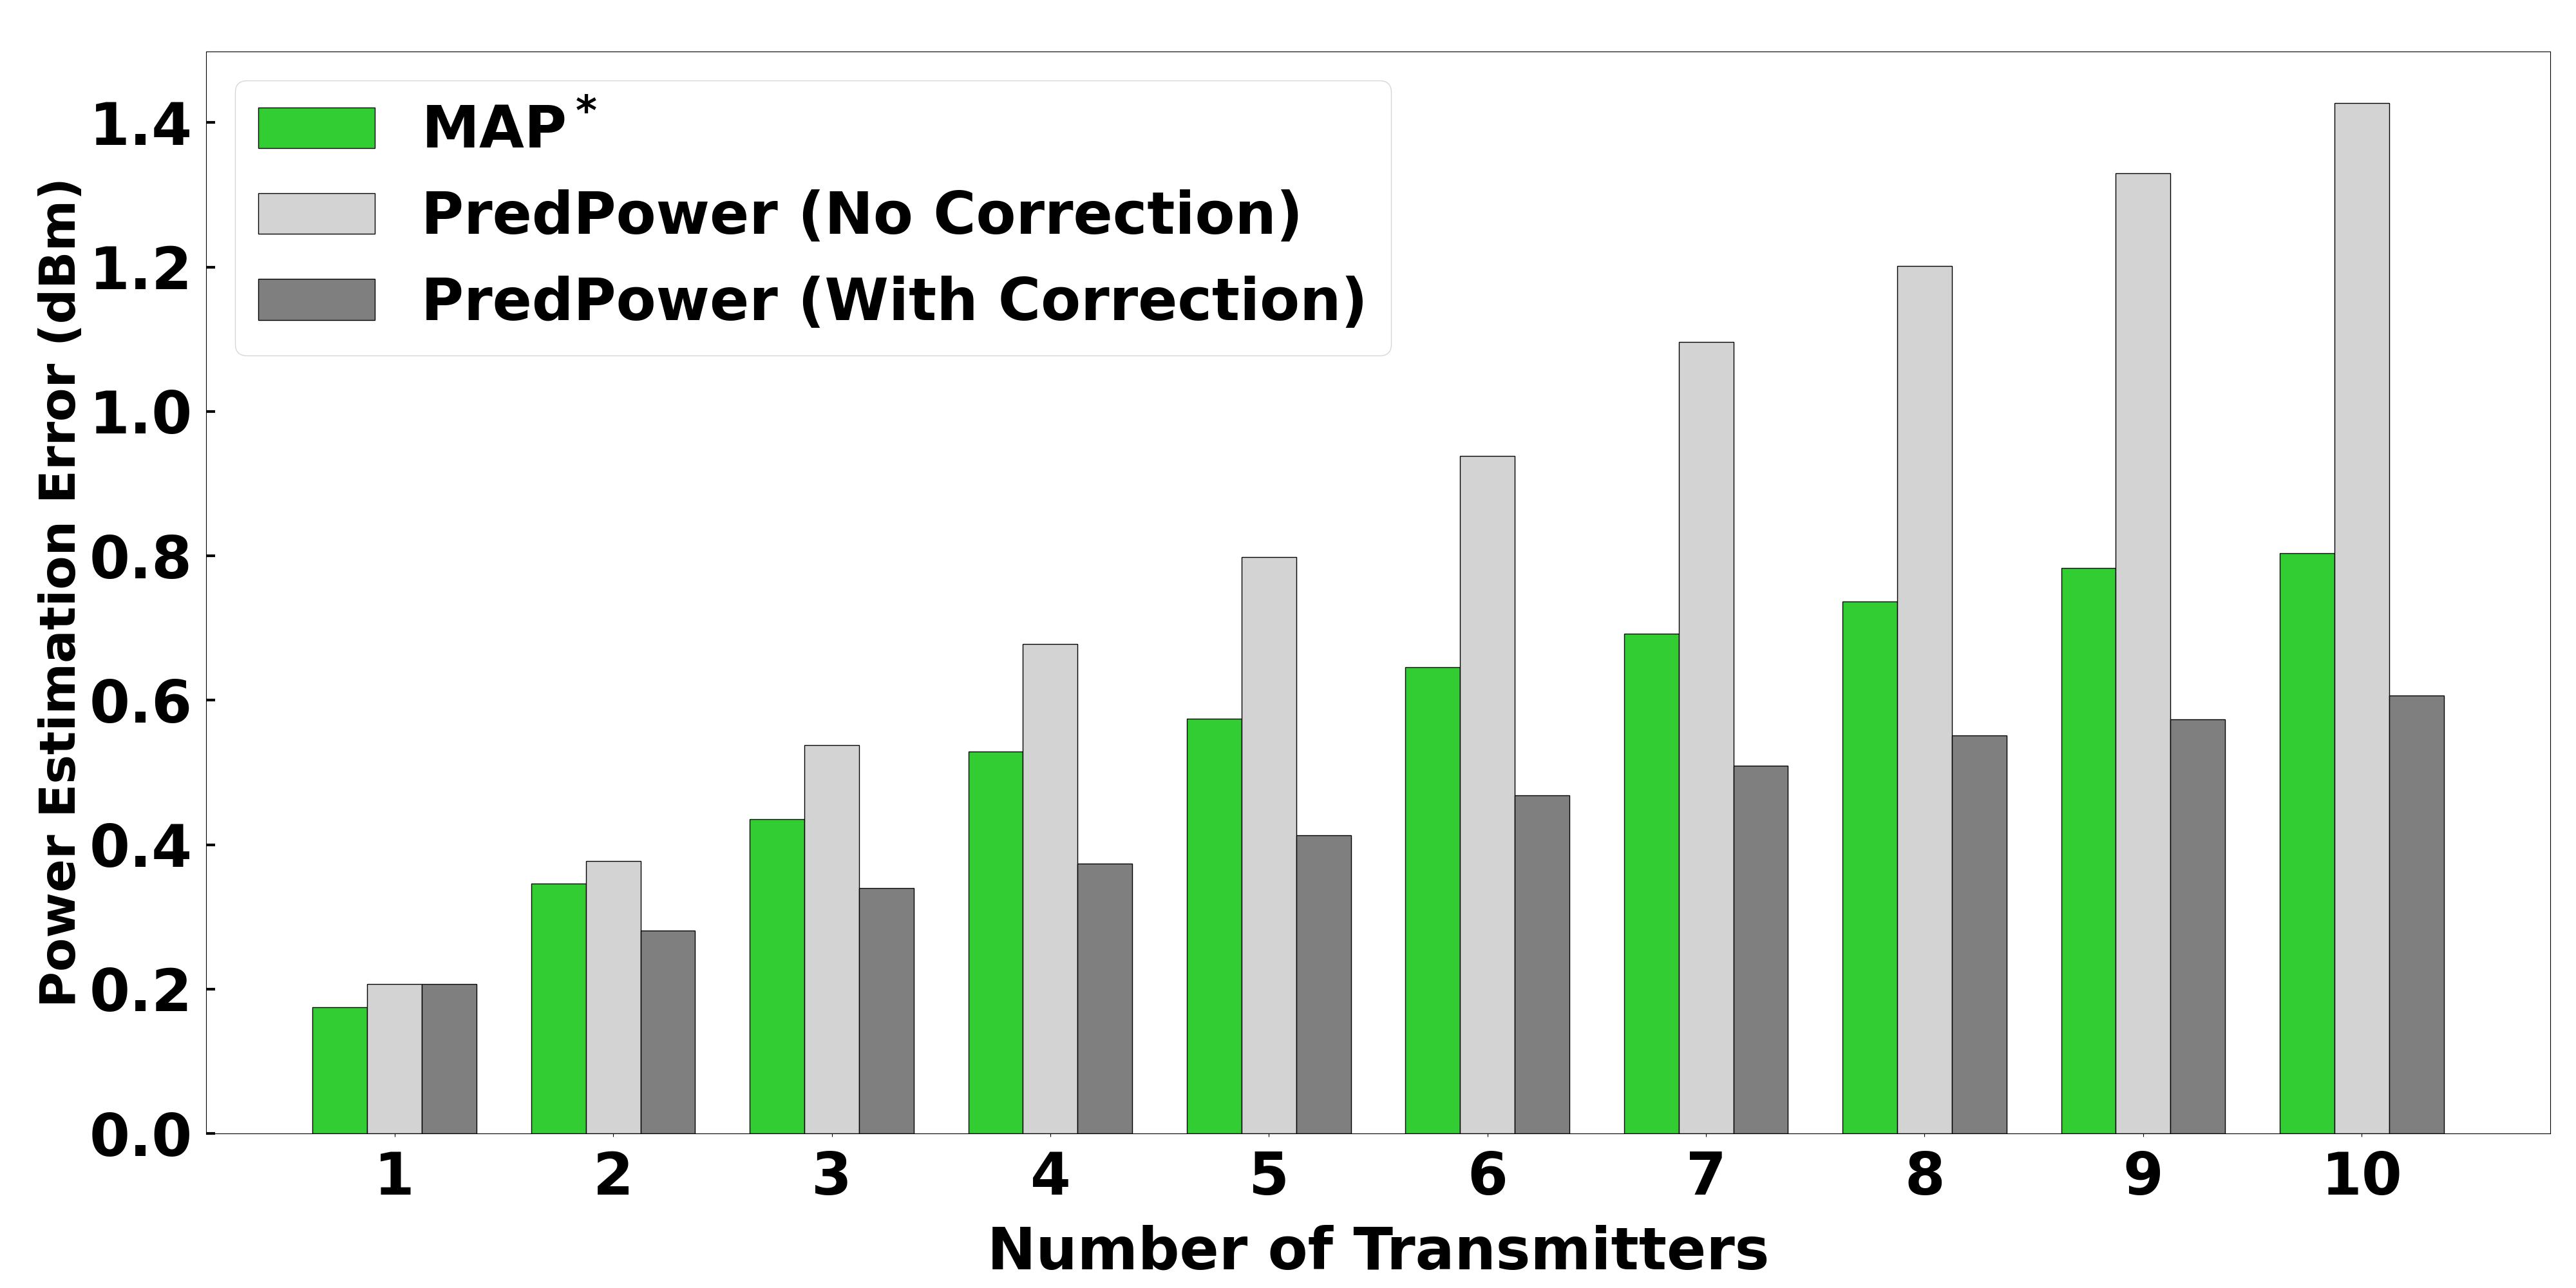
\includegraphics[width=0.75\textwidth]{chapters/wowmom-pmc/figures/logdist-powererror_varyintru.png}
    \caption{The transmitter power estimation error of \map, \power with and without correction in Log-distance model for varying number of intruders}
    \label{fig:logdistance-multiTXpower}
\end{figure}
\begin{figure}[t]
    \centering
    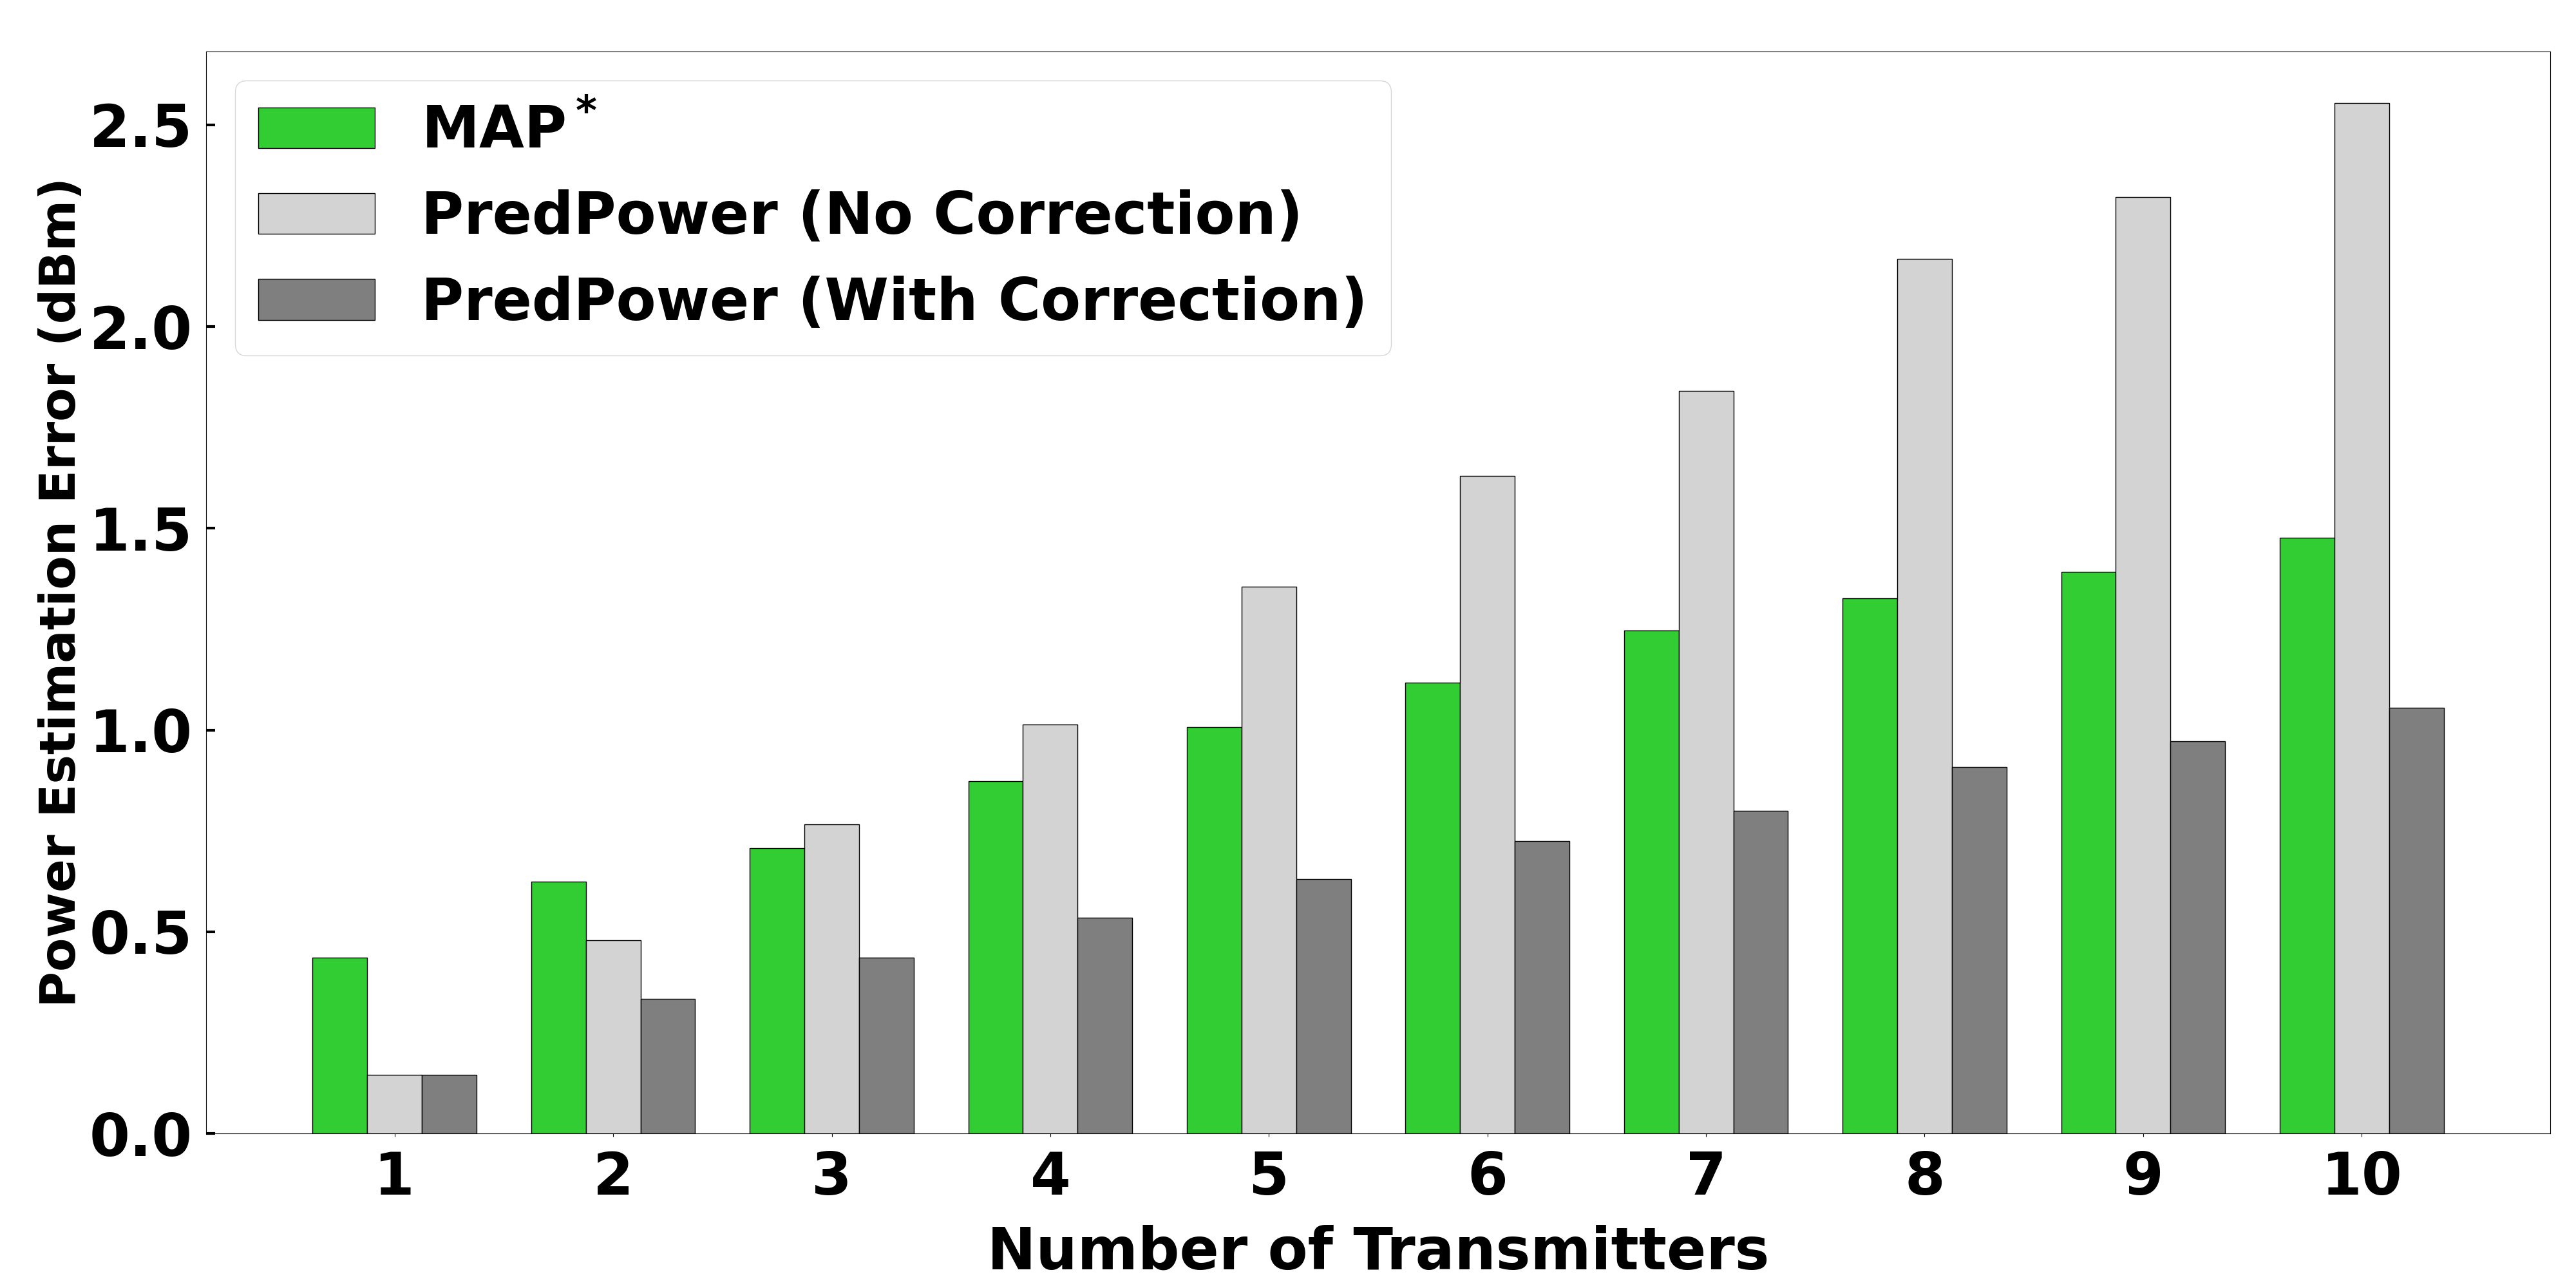
\includegraphics[width=0.75\textwidth]{chapters/wowmom-pmc/figures/splat-powererror_varyintru.png}
    \vspace{-0.1in}
    \caption{The transmitter power estimation error of \map,  \power with and without correction in Longley--Rice Irregular Terrain with Obstruction Model (SPLAT!) for varying number of intruders.}
    \label{fig:splat-multiTXpower}
\end{figure}
%%%
Figure~\ref{fig:logdistance-multiTXpower} shows the power estimation error of three methods with a varying number of transmitters while the sensor density is 6\%.
In this figure, \map is the best only when the number of transmitters is one (which is consistent with Fig~\ref{fig:singleTXpower}(a)).
Also the number of transmitters is one is the only case when \power with correction and without correction has the same performance.
This is also expected because there is no need to error correction when there is only one transmitter in the area.
In all other cases, we see that \power with error correction is the best, \power without error correction  is the worst, and \map is in the middle.
In Figure~\ref{fig:splat-multiTXpower}, which shows experiment results running in the SPLAT! propagation model, we see a similar pattern compared to Figure~\ref{fig:logdistance-multiTXpower}.
The difference is that \power with error correction is always the best and the power error is larger than the log-distance model scenario.
For example in Figure~\ref{fig:logdistance-multiTXpower}, the power estimation error for \power with error correction goes up to 0.6 dB, where as in Figure~\ref{fig:splat-multiTXpower}, the error goes up to 1 dB.







\subsection{Evaluation over Testbed Data}
\label{subsec:ipsn}
In this subsection, we show that our \our performs well in real-world collected data.
For this, we repurpose our testbed data from~\cite{ipsn20-mtl} as described below. We start with describing our testbed data from~\cite{ipsn20-mtl}.

\para{Testbed Data.}
In \cite{ipsn20-mtl}, we conducted a testbed in an outdoor parking area of $32m\times 32m$ large.\footnote{Dataset publicly available at: \url{https://github.com/Wings-Lab/IPSN-2020-data}}
Each grid cell has a size of $3.2m \times 3.2m$, with the grid size being $10\times 10$.
We place a total of 18 sensors on the ground.
The sensors consist of Odroid-C2 (a single-board computer) connected to an RTL-SDR dongle and the RTL-SDR connects to dipole antennas.
The transmitters are USRP or HackRF connecting to a laptop.
We collect raw Inphase-Quadrature (I/Q) samples from the RTL-SDR at the 915 MHz ISM band.
We perform FFT on the I/Q samples with a bin size of 256 samples to get the signal power values, and then utilize the mean and standard deviation of the power at frequency 915 MHz reported from each of the sensors.

\para{Transforming the Data from $10 \times 10$ to $100 \times 100$ Grid.}
Note that \our's input requires a $100\times 100$ input, while the above data is over a
 $10\times 10$ grid. Also, the sensor density in the above data is 18\%, while we desire a sensor
 density of around 4-6\% to have a fair comparison with our simulation based evaluations in previous subsections. To achieve these objectives, we transform the above $10 \times 10$ data to a $100 \times 100$ grid data in two steps as follows.
% So, the second goal is to transform the sensor density to fall in the middle of the sensor density ranged used in the simulated based evaluations, which is 1\% to 10\%, for a fair comparison.
% Duplication and increasing granularity are two methods we use to transform the testbed data.
% If we only duplicate the $10\times10$ grid a hundred times to $100\times100$, then the sensor density will remain at 18\%, which is too high.
% If we only increase the granularity to $100\times100$, then the sensor density will drop to 0.18\%, which is too low.
%Thus, we use a combination of the two methods to satisfy the two goals, as described in the following two steps.}
\begin{enumerate}
    \item Increase the data granularity from $10 \times 10$ to $20\times 20$, by dividing each cell into $2 \times 2$ cells; we randomly pick one of these four smaller cells to represent the original cell (i.e., to place the sensor if it existed in the original cell). See the red-bordered boxes in Fig.~\ref{fig:testbed}(a)-(b). We refer to the full $20 \times 20$ grid as a \emph{tile}.
    \item Now, we duplicate the $20\times20$ tile $25$ times using a $5 \times 5$ pattern to generate a  $100 \times 100$ grid. See Fig.~\ref{fig:testbed}(b)-(c).
\end{enumerate}
The above steps effectively increase the area from the original $32m\times32m$ to $160m\times160m$. 
Note that the first step above only splits each original cell into four smaller cells without increasing the whole area size.
The $100\times100$ grid will have a sensor density of 4.5\% and each grid cell represents an area of $1.6m\times1.6m$.



%\blue{Note that the grid size is the only relevance during the grid transformation, not the area that the grid represents.
%However, after transforming the $10\times10$ grid into a $100\times100$ grid, the new grid will represent a different area.
% A tile's area is $32m\times32m$ large, which is the same as the original $10\times10$ grid. 
% But after duplicating to 25 tiles, the new $100\times100$ grid will represents a larger area of $160m\times160m$.
% The new $100\times100$ size grid will have a sensor density of 4.5\% and each grid cell represents an area of $1.6m\times1.6m$.}

We note that the second duplication step can introduce inaccurate sensor readings at the tile's ``edges", due to 
any transmitters from adjoining tiles. To circumvent this issue, we place {\em transmitters} only within the internal
$10 \times 10$ cells of each $20 \times 20$ tile (i.e., avoid placing a transmitter on the five-cell edge of each tile). This
yields a total of 2500 potential positions to place a transmitter in the final $100 \times 100$ grid. 
With the above setting, we generate training and testing datasets consisting of 25,000 and 12,500 samples respectively.
% The transmitters, however, cannot be placed at every possible location.
% For every tile, the transmitters will not be located at the edges.
% Because if so, there will be no RSSI observation data for the sensors at the edge of neighbor tiles.
% The edge's width equals to five cells. 
% When a transmitter is inside a tile, only the sensors inside the same tile will receive some signals from that transmitter (the sensors at the neighbor tile's edge will be ignored).
% \eat{Also, the increase of granularity (step 1) leads to only every one in four cells are legit sensor locations, these legit sensor locations will also be the legit transmitter locations.
% So for each tile, the legit cell locations for a transmitter is $(20-5\times2)^2 = 100$.
% Given 25 tiles, the total legit cell locations for a placing a transmitter is $100\times25=2500$.
% For multiple transmitters, they are randomly picked from these 2500 grid cells (a transmitter's location is still continuous inside the grid cell).
% A sensor receives an aggregated signal power from multiple transmitters.
%Thus, we can generate a $100\times100$ size input data that can be used by \our from a much smaller data of size $10\times10$ with a combination of granularity increase and duplication.}

\begin{figure}[t]
    \centering
    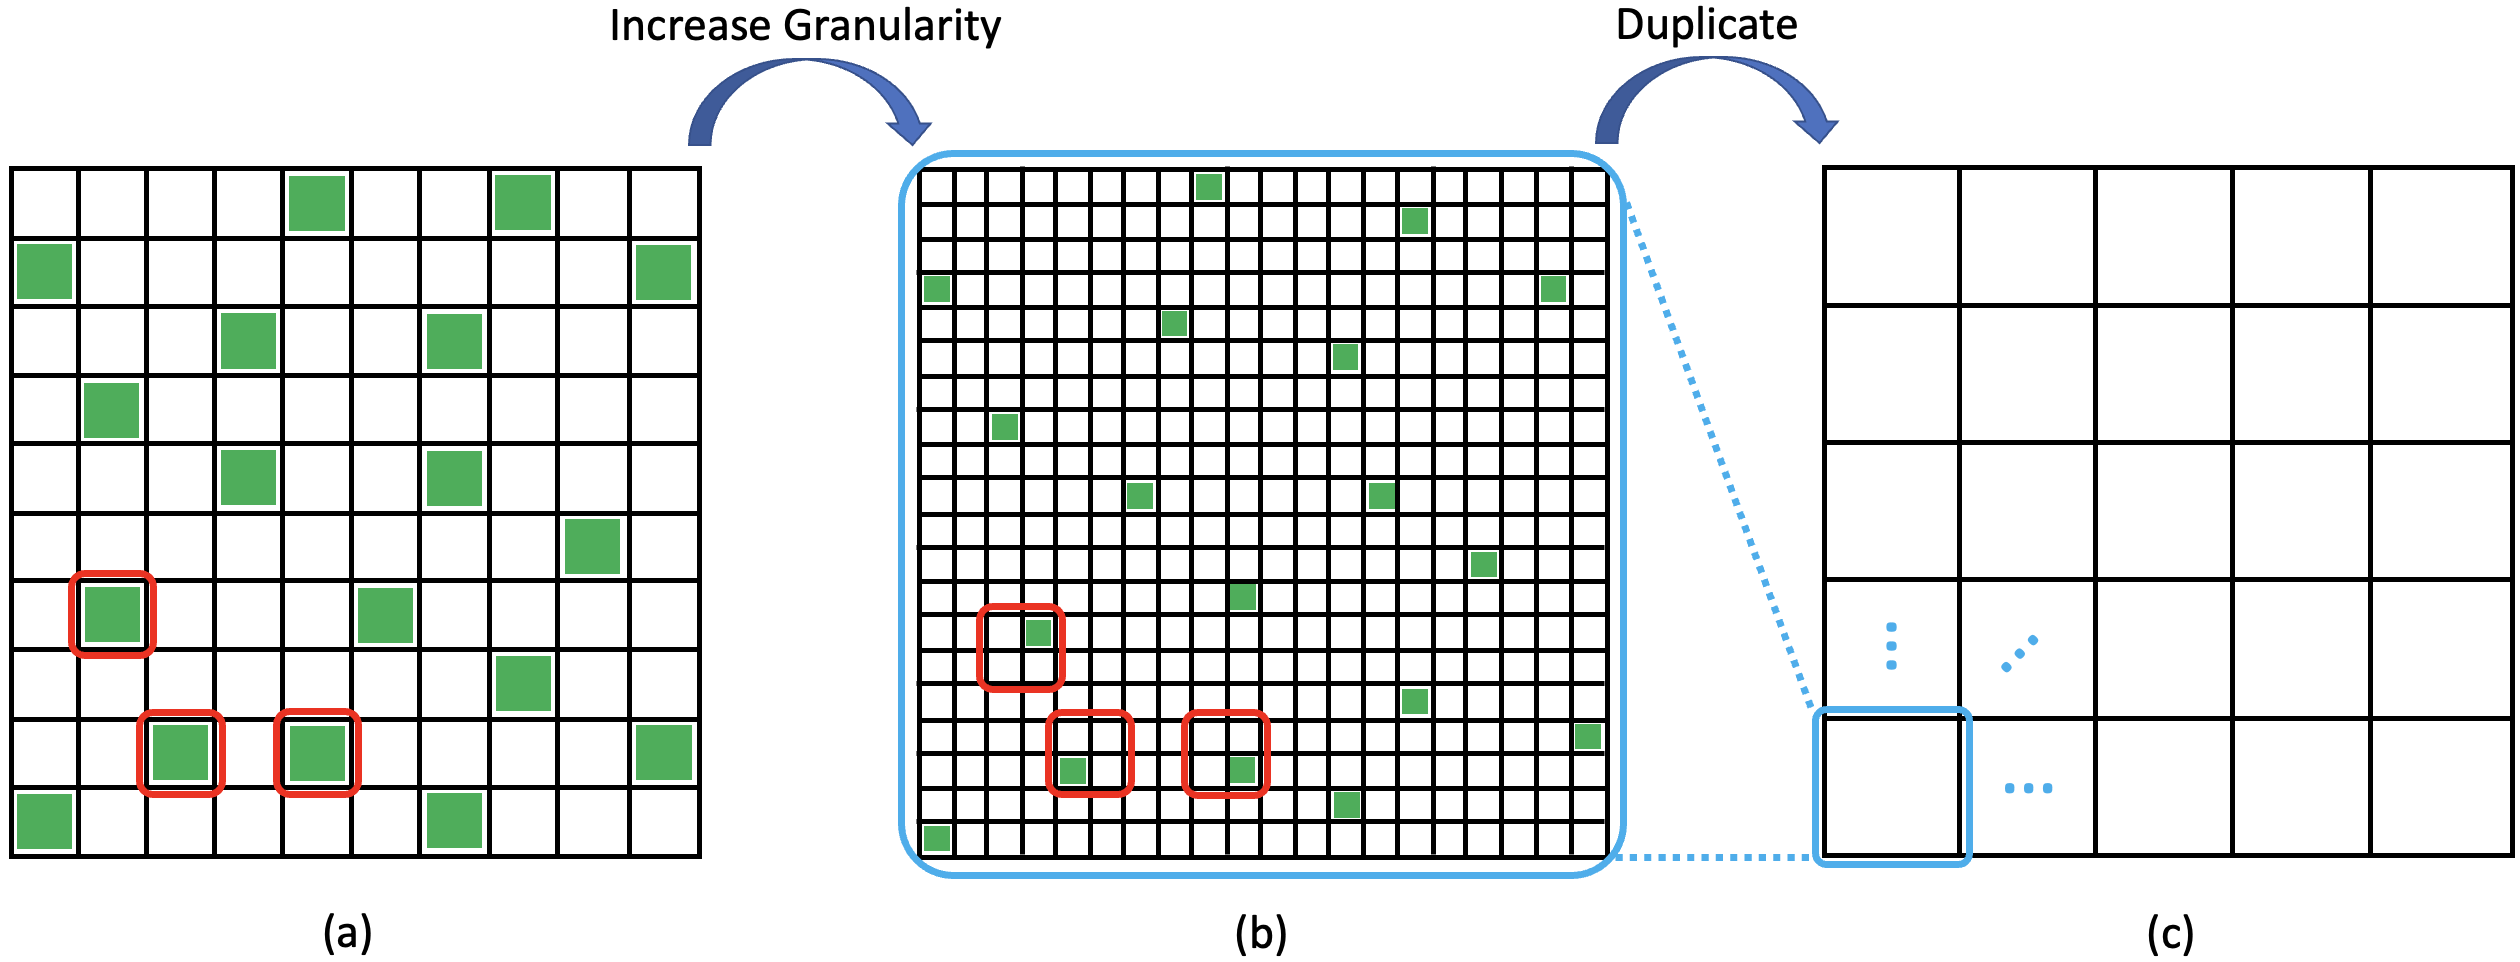
\includegraphics[width=0.98\textwidth]{chapters/wowmom-pmc/figures/testbed.png}
    \caption{(a). The original $10\times10$ testbed grid with 18 sensors (green cells) representing a $32m \times 32m$ area. (b). The $20\times20$ grid (a tile) obtained by replacing each original cell by $2 \times 2$ smaller cells; a sensor, if present in the original cell, is placed in a random cell within the  $2\times2$ grid (see the green cells). (c). The final $100\times100$ grid obtained by duplicating the $20\times20$ tile 25 times using a $5\times5$ pattern. The final geographic area is $160m\times160m$.}
    \label{fig:testbed}
\end{figure}

\begin{figure}
    \centering
    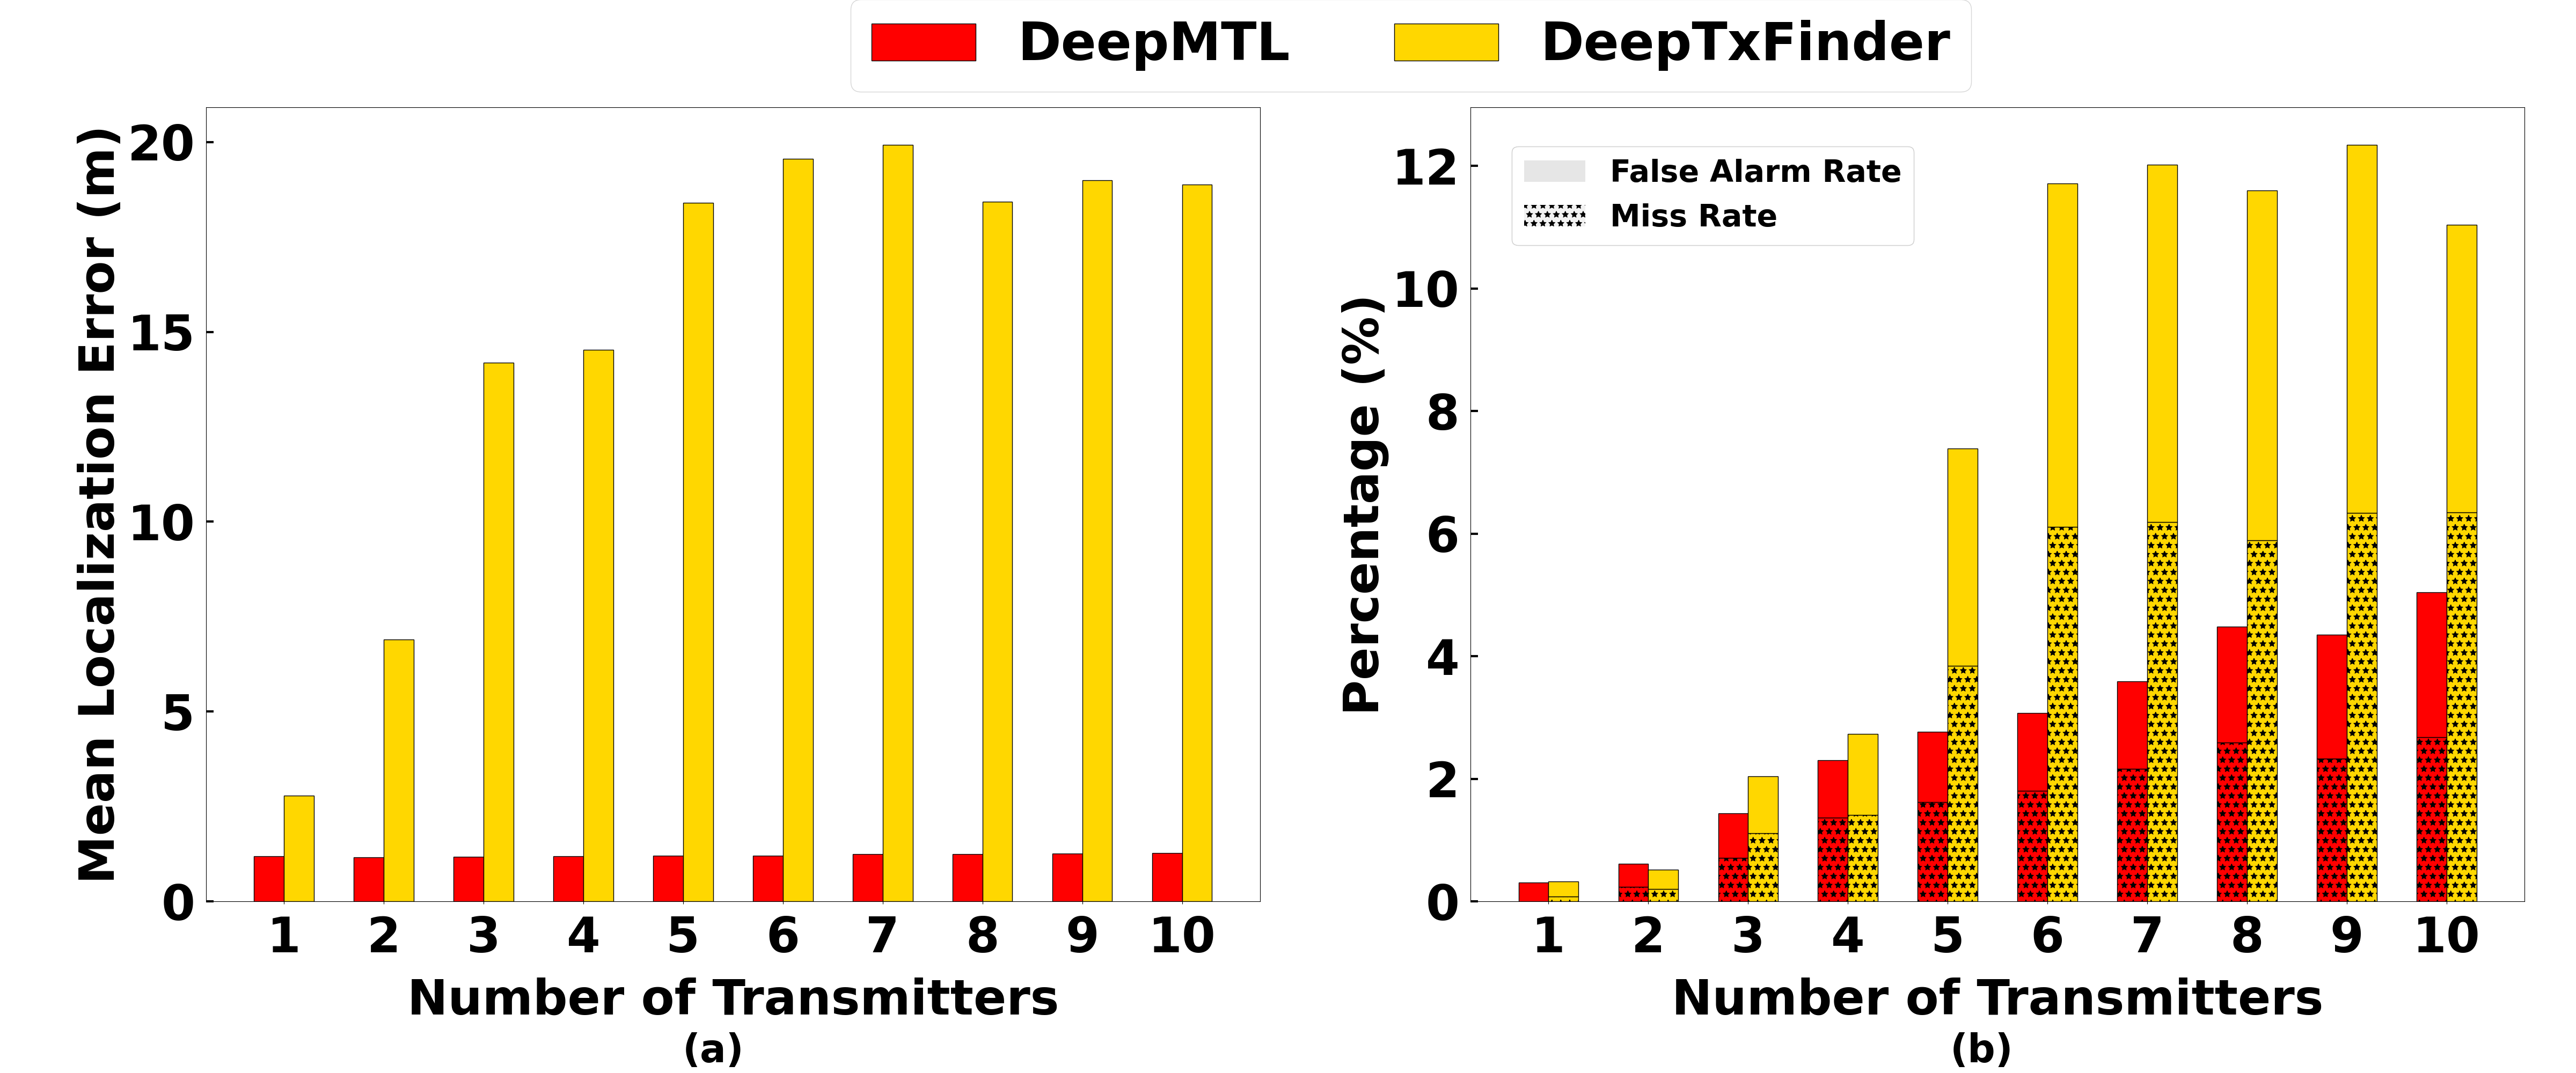
\includegraphics[width=0.95\textwidth]{chapters/wowmom-pmc/figures/ipsn_testbed-error_false_miss_vary_numintru.png}
    \caption{The localization error (a), false alarm rate and miss rate (b) of \our and \deeptx in a real world collected data for varying number of intruders.}
    \label{fig:ipsn}
\end{figure}

\para{Testbed Results.}
The performance of \our on this real world based data is shown in Fig.~\ref{fig:ipsn}.
Compared to \deeptx, \our is significantly better in localization error and false alarm rate and miss rate in almost all cases, which aligns to the results in the previous subsections based on data generated from either log-distance model or SPLAT!.
The localization error of \our in Fig.~\ref{fig:ipsn}(a) is around 1.3 meters.
The error increases mildly with the increase in the number of transmitters.
The localization error in the testbed data is smaller compared to both log-distance data results (Fig.~\ref{fig:logdist-error-vary_numintru}) and SPLAT! data results (Fig.~\ref{fig:splat-error-vary_numintru}).
This is because a grid cell here is representing a smaller area.
In the log-distance data, the localization error is roughly one-fourth the side length of the grid cell. 
In the SPLAT! data result, the localization error is roughly half the side length of its grid length.
In the testbed data, the localization is roughly eighty percent the side length of a grid cell.
So the localization error in the testbed data is the highest relative to the length of a grid cell it represents.
The sum of false alarm rate and miss rate is 3\% when the number of transmitters is five and is 5\% when the number of transmitters is ten.
The results are a little bit worse than the results in the SPLAT! data (Fig.~\ref{fig:splat-missfalse-vary-numintru}), where the sum is 2\% for five transmitters and 4\% for ten transmitters.


\section{Related Work}
\label{sec:wowmom-related}
\para{Spectrum sensing} is usually being realized by some distributed crowdsourced low-cost sensors. 
Electrosense~\cite{electrosense} and its follow up work Skysense \cite{mobisys20-skysense} are typical work of spectrum sensing.
In this crowdsourced sensing paradigm~\cite{chakraborty2017specsense}, sensors collect I/Q samples (in-phase and quadrature components of raw signals) and compute PSD (power spectral density), which is RSS.
Crowdsourced low-cost sensors do not have the capability to collect AoA (angle of arrival) data because it requires more expensive antenna arrays.
They also do not have the capability to collect ToA (time of arrival) data because it requires the transmission of a wide-band known sequence~\cite{pimrc2021-localize}, which is impossible in the case of localizing (blind) intruders.
Spectrum sensing platforms serve as the foundation of the spectrum applications, and transmitter localization is one of the main applications.
Other applications include signal classification~\cite{toccn18-sigclassify}, spectrum anomaly detection~\cite{ben-zhao}, sensor selection~\cite{ton-sensorselect,bhattacharya2022fast}, spectral occupancy estimation~\cite{mobicom21-deepradar}, etc.

\para{Transmitter localization.} Localization of an intruder in a field using sensor observations has been widely studied, but most of the works have focused on
localization of a single intruder~\cite{infocom18-spectrum,dutta2016see}.
%%%%%
In general, to localize multiple intruders, the main challenge comes
from the need to ``separate'' powers at the sensors~\cite{mobicom-30},
i.e., to divide the total received power into power received from
individual intruders. Blind source separation is a very challenging
problem; only very limited settings allow for known
techniques using sophisticated receivers~\cite{freq-sig,ben-zhao}.
%%%
We note that (indoor) localization of a
  device~\cite{infocom00-radar} based on signals received from multiple reference points (e.g, WiFi access
  points) is a quite different problem
  (see~\cite{zafari-19} for a recent survey), as the signals from
  reference points remain separate, and localization or tracking of multiple
  devices can be done independently.
  Recent works on multi-target localization/tracking such as~\cite{ipsn19-multipassive} are different in the way that targets are passive, instead of active transmitters in the \mtl problem.
Among other related works,~\cite{multi-tx-dyspan-19} addresses the challenge of handling time-skewed sensors observations in the MTL problem.
%%%%%%%%%%%%%%%%%%%%%%%
\eat{In absence of blind separation methods, to the best of our knowledge,
only a few works have addressed multiple intruder(s) localization. 
In particular,
(i)\splot~\cite{mobicom17-splot} decomposes the multi-transmitter
localization problem to multiple single-transmitter localization
problems based on the sensors with highest of readings in a
neighborhood, (ii)~\cite{clustering} uses a clustering-based approach, (iii)~\cite{Quasi-EM} uses an
EM-based approach, (iv) \map~\cite{ipsn20-mtl}, uses 
a hypotheses-based Bayesian
approach in conjunction with a divide-and-conquer strategy to first localize 
``isolated"  intruders and then localize the remaining intruders,
(v)We note that the techniques of~\cite{mobicom17-splot,Quasi-EM} assume a propagation
model, while that of~\cite{clustering,Quasi-EM} require a priori
knowledge of the number of intruders present. 
Schemes in~\cite{Quasi-EM} and~\cite{clustering} have been shown inferior in performance in~\cite{mobicom17-splot,ipsn20-mtl}.
}

\para{Wireless localization} techniques mainly fall into two categories: geometry mapping and fingerprinting-based.
Geometry mapping mainly has two subcategories: ranging-based such as trilateration (via RSS/RSSI, ToA~\cite{zongxing2022tracking}, TDoA) and direction-based such as triangulation (via AoA).
Fingerprinting-based methods can use all signal physical measurements including but not limited to amplitude, RSS/RSSI, ToA, TDoA, and AoA.
Whenever deep learning is used for localization, it can be considered as a fingerprinting-based method, since it requires a 
training phase to survey the area of interest and a testing phase to search for (predict) the most likely location.

\para{Deep learning for wireless localization}. 
Quite a few recent works have harnessed the power of deep learning in the general topic of localization.
E.g., DeepFi in~\cite{DeepFi2016} designs a restricted Bolzmann machine that localizes a single target using WiFi CSI amplitude data. 
DLoc in~\cite{mobicom20-deeploc} uses WiFi CSI data as well. 
Its novelty is to transform CSI data into an image and then uses an image-to-image translation method to localize a single target.~MonoDCell 
in~\cite{sigspatial19-monodcell} designs an LSTM that localizes a single target in indoor environment using cellular RSS data.
~\cite{pimrc2021-localize} designs a three-layer neural network that locations a single transmitter.~\deeptx in~\cite{icccn20-deeptxfinder} 
uses CNN to address the same \mtl problem using RSS data in this chapter.

\para{Transmitter Power Estimation.} There are several works that estimate the transmission power of a single transmitter.
~\cite{PowerEstimate2010Zafer} studies the ``blind" estimation of transmission power based on received-power measurements at 
multiple cooperative sensor nodes using maximum likelihood estimation. Blind means there is no prior knowledge of the location of the 
transmitter or transmit power.~\cite{Ureten2011powerlocation} propose an iterative technique that jointly estimate the location and 
power of a single primary transmitter.
In~\cite{icoin2007-powerposition}, the primary transmitter location and power is jointly estimated by a constrained optimization method.
~\cite{ipsn20-mtl} uses the maximum likelihood estimation method to estimate the power of an isolated single transmitter and 
adopts an online learning method to estimate the power of multiple close by transmitters simultaneously.

\para{Machine learning empowered applications.} Machine learning techniques have empowered many applications.
Social media bots can be detected effectively via behavioral patterns~\cite{wu2023botshape} and metric learning~\cite{wu2023bottrinet}.
Machine learning is used to enhance the portfolio construction based on PolyModel theory~\cite{siqiao2023}.
AI-assisted audio command recognition enables collaborative human-robot drone inspection of bridges~\cite{yuli_thesis}.
In~\cite{ziheng_thesis,ziheng2022}, algorithms are developed to make machine learning models more transparent, accountable and explainable~\cite{ziheng_relax,ziheng2023dark}.
Network function virtualization~\cite{wang2023thesis,wang2022quadrant,wang2020slos} has great potential in low-performance edge devices~\cite{wang2023scheduling}
as more applications and ISP functionalities are expected to be offloaded to edge clouds~\cite{wang2021galleon,wang2023pinolo}.
Machine learning can help the simulation and analyses of multi-platelet recruitment simulation~\cite{yicong_thesis}.
In~\cite{peineng2023}, a machine learning-guided imaging approach is used to segment platelet geometries and quantify adhesion dynamics parameters.
DeepVS~\cite{zongxing2022dl} combines 1D CNN and attention models to exploit local features and temporal correlations to improve RF-based vital signs sensing.
A LSTM encoder-decoder model is proposed to generate Chinese poetry~\cite{yubo2017text}.

\para{RF sensing for mobile health and edge computing.}
RF sensing enables some important mobile health applications such as heart and respiratory rate monitoring~\cite{zongxing2022uwb,zongxing2022measure}. 
RF based solutions support practical and longitudinal respiration monitoring owing to their non-invasive nature~\cite{zongxing2023rf,zongxing2021uwb}.
~\cite{zongxing2024rfq} proposed a robust RF-based respiration monitoring.
Low quality RF sensing data will negatively affect the sensing task, thus reliable signal quality detection is crucial~\cite{zongxing2021quality}.
Apart from RF sensing, acoustic sensing can also enable important applications such as face authentication~\cite{zongxing2019face,zongxing2022face}.
In traditional wireless sensor networks, the sensing data is uploaded (via wireless) to a centralized server~\cite{yubo2023blockchain} and the server process the sensing data.
In an emerging computing paradigm called edge computing, however, sensing data is processed locally on the resource constrained sensors, 
e.g., on-device machine learning~\cite{yubo2020ondevice,yubo2022demo,yubo2019ondevice}.
Thus, various works target to scale up task execution on resource-constrained systems~\cite{yubo_thesis}, such as 
SmartOn~\cite{yubo2021smarton}, Antler~\cite{yubo2023efficient} and intermittently-powered systems~\cite{yubo2023audio,yubo2023intermittent}.



%Both DLoc and \deeptx also represent the explore the usage of CNN in the wireless localization problem by representing the input wireless data as images.
%We also use images to represent wireless data (see Fig. \ref{fig:input}) and harness the power of deep learning on top of that.
%Below, we introduce our high-level approach.
  
  %, and (ii)~\cite{info-20} that addresses the sensor selection optimization problem.
  

  
%%%%%
%\blue{Other related works include:~\cite{mobicom-22} where sensors are
%  on mobile and controlled robots,~\cite{mobi-25} focusses on spectrum
%  allocation via spectrum hole detection in presence of background 
%  transmitters.} \red{HG: Remove this sentence?}

%% Online selection of sensors: ipsn-04, .... latency vs. energy .. since,
%% latency is equally critical, ... we dont want to run it for every intruder ... 
%% Similarly,
%% \cite{krause2008near} shows that minimizing uncertainty in a gaussian
%% process is submodular, and thus greedy selection provides a bounded
%% solution to the optimal.

%% Multiple studies have studied sensor selection to maximize the
%% accuracy of detection of some event \cite{rowaihy2007survey}.

%% For
%% example, \cite{joshi2009sensor} provides a heuristic for sensor
%% selection by forming a convex optimization problem.  However, it uses
%% a different metric to measure the accuracy of detection.
%% %%%%
%% Other studies, such as
%% \cite{shamaiah2010greedy} and \cite{bian2006utility} have proposed
%% leveraging submodularity to select sensors.  

%% There are also studies in the active learning literature that focus on
%% online selection.  For example, \cite{yuxin-when} limits the mutual
%% information while selecting the minimum possible number of sensors.
%% \cite{krause2012near} shows that mutual information in sensor
%% selection is submodular in the absence of noise and propose a
%% probabilistic greedy algorithm by leveraging it.
%% \cite{golovin2011adaptive} proposes the concept of adaptive
%% submodularity that generalizes the greedy approximation to online
%% selection. Our online selection algorithm builds upon these studies to
%% limit the number of sensors while maximizing the mutual information.
%% However, in the presence of noise, mutual information is not adaptive
%% submodular in nature.  Thus, our work modifies the algorithm discussed
%% in \cite{yuxin-when} to make it suitable for our use case.

\section{Conclusion}

In this chapter, we have designed and developed a novel deep-learning-based scheme (\our) for
the multiple transmitter localization (\mtl) problem.
We extended this problem to localizing the intruders in the presence of authorized users and developed a novel technique to solve it. 
We also developed a novel technique that can solve the multiple transmitter power estimation (\mtpe) problem.
Solving the general \mtl and \mtpe are both achieved by utilizing our robust \our as a building block. 
We evaluated all our methods extensively through data simulated from two propagation models as well as small-scale data collected from a real-world testbed. 
Our developed technique outperforms prior approaches by a significant margin in all performance metrics.
%we would like to improve generalization by investigating the scenario when training and testing datasets are generated from two different geographical areas. 
%Lastly, for very large number of transmitters, we would like to explore crowd counting techniques, borrowing more from the computer vision community.}


%In our 
%For future work, we will try to train our two steps \imgimg and \yolocust end-to-end, instead of separately as we did currently.
%Also, we would like to evaluate our method in real world testbeds and see if the performance math the performance done in simulations.
% \section{Acknowledgements}
This work is supported by National Science Foundation grants CNS-1642965, CNS-1815306, and CNS-2128187. The authors would like to thank the reviewers for the valuable feedback and advice.

\chapter{Quantum Sensor Network Algorithms for Transmitter Localization}
\label{chap:qce}

A quantum sensor (QS) is able to measure various physical phenomena with extreme sensitivity.
QSs have been used in several applications such as atomic interferometers, but few applications of a quantum sensor network (QSN) have been proposed or developed.
We look at a natural application of QSN---localization of an event (in particular, of a wireless signal transmitter).
In this paper, we develop effective quantum-based techniques for the localization of a transmitter using a QSN.

Our approaches pose the localization problem as a well-studied quantum state discrimination (QSD) problem and address the challenges in its application to the localization problem. 
In particular, a quantum state discrimination solution can suffer from a high probability of 
error, especially when the number of states (i.e., the number of potential transmitter locations in our case) can be high. 
We address this challenge by developing a two-level localization approach, which localizes the transmitter at a coarser granularity in the first level, and then, in a finer granularity in the second level. 
%%%%%%%%%%%%%%
We address the additional challenge of the impracticality of general measurements by 
developing new schemes that replace the QSD's measurement operator with a trained parameterized hybrid quantum-classical circuit.
%%%%%%%%%%%%%%%
Our evaluation results using a custom-built simulator show that our best scheme is able to 
achieve meter-level (1-5m) localization accuracy; 
in the case of discrete locations, 
it achieves near-perfect (99-100\%) classification accuracy. 
\section{Introduction}

Quantum sensors, being strongly sensitive to external disturbances, are able to measure various physical phenomena with extreme sensitivity.
These quantum sensors interact with the environment and have the environment phenomenon or parameters encoded in their state~\cite{RevModPhys.quantumsensing}.
In~\cite{kaiwen1,kaiwen2}, multiplexer technologies are proposed to facilitate the readout of large (nearly 2000) 
arrays of superconducting transition-edge sensor bolometers (i.e., quantum detectors), largely accelerating the development of astronomy.
A group of distributed quantum sensors, if prepared in an appropriate entangled state, can further enhance the estimation of a single continuous parameter, improving the standard deviation of measurement by a factor of $1/\sqrt{m}$ for $m$ sensors (Heisenberg limit)~\cite{Giovannetti_2011}.
\eat{Recently, experimental physicists successfully demonstrated a reconfigurable distributed radio-frequency photonic sensor network~\cite{PRL20-qsn,arizona21-thesis} that utilizes squeezed quantum state and entanglement to enhance sensing of radio signals.}
% The experiments establish a connection between the entanglement structure and the achievable quantum advantage in different distributed sensing problems.

Recently, many protocols have been developed for the estimation of a single 
parameter or multiple independent parameters~\cite{Giovannetti_2011,mpe_2018} using one or multiple (possibly, entangled) sensors. 
But, the use of a distributed set of quantum sensors working collaboratively 
to estimate more complex physical/environmental phenomena, as in many classical
sensor network applications~\cite{tsn17-water, sensys10-health,mobicom03-sensor}, 
has not been explored much.
% In this paper, we develop a scheme for the localization of events using a quantum sensor network (QSN);
In this paper, we explore a potential quantum sensor network application--- localization of events.
In particular, we develop effective techniques 
for radio frequency (RF) transmitter localization and thus demonstrate the promise of QSNs in the accurate localization of events. Our motivation for choosing 
RF transmitter localization as the event localization 
application is driven by the significance of transmitter localization
in  wireless/mobile applications and recent advances in quantum sensor
technologies for RF signal detection (see \S\ref{sec:quantum_problem}).

\begin{figure*}[t]
    \centering
    \includegraphics[width=0.95\textwidth]{chapters/qce/figures/overall.png}
    \caption{Overall architecture of using a QSN to localize a transmitter. 
    % The transmitter's location is at $(x, y)$ and the estimated location is $(x', y')$
    }
    \label{fig:quantumoverall}
\end{figure*}

\para{Transmitter Localization using QSNs.}
Our approach to
transmitter localization using QSNs essentially involves posing
the localization problem as a quantum state discrimination
(QSD) problem~\cite{bergou-review-2007} which is to identify the specific state a given
quantum state is in (from a given set of states in which the
system can be) by performing quantum measurements on the
given quantum system. The overall architecture is illustrated in
Fig.~\ref{fig:quantumoverall}. 
First, a probe state is generated and distributed to the
QSN. Then, once the quantum sensors have been impacted
(i.e., the overall quantum state changed) due to the transmission
from the transmitter’s signal, an appropriate quantum measurement 
is made on the quantum state of the network.
The outcome of the measurement determines the quantum
state, and thus, the location of the transmitter. 
However, the
above process can be erroneous, as solving 
the QSD problem even optimally
can incur a certain probability of (classification/discrimination)  error.
This paper’s goal is to develop an approach with a 
minimal localization error. 
%%%%%%%%%
In that context, our
developed schemes in this paper are based on two ideas that extend
the above basic QSD-based approach: 
\begin{enumerate}
    \item We use a two-level approach
that localizes the transmitter in two stages: first, at a coarse level
using a set of sensors over the entire area, and then, at a fine level
within the ``block'' determined by the first level. 
\item In addition, we circumvent the challenge of implementing a general
measurement operation, by instead using a trained parameterized 
hybrid quantum-classical circuit that essentially implements the 
measurement operation and predicts the transmitter location from
quantum sensor data.
\end{enumerate}
Our evaluation results show that our best scheme (which combines the above two ideas) is able to achieve meter-level (1-5m) localization accuracy; in case of discrete locations, it achieves near-perfect (99-100\%) classification accuracy. 

\para{Contributions.} 
In the above context, we make the following contributions. 
\begin{enumerate}
    \item We model the transmitter localization problem as a well-studied quantum state discrimination (QSD) problem, which allows us to develop viable transmitter localization schemes using quantum sensors. 
 
    \item 
    We design two high-level schemes to localize a transmitter in a given area deployed with a quantum sensor network.
     The first scheme is based on solving an appropriate quantum state discrimination problem using a global measurement, while the second scheme uses a trained hybrid quantum-classical circuit to process the quantum sensor data. Within the above high-level schemes, we also introduce a two-level localization scheme to improve the performance of the basic one-level schemes.
  
    \item 
    To evaluate our schemes, we model how a quantum sensor's state evolves due to RF signals from a transmitter at a certain distance. Using this model, we 
     evaluate our localization schemes and demonstrate their effectiveness in our custom-built simulator.
\end{enumerate}

% \magenta{To the best of our knowledge, ours is one of the two recent works to investigate and develop techniques for event-localization problems using a collaborative 
% network of quantum sensors. 
% The other work is~\cite{PR22-quantum_positioning} who uses a small network of four quantum sensors to localize an incoming signal by estimating the signal's angle of arrival to different sensors.
% ~\cite{PR22-quantum_positioning} introduced the concept, however, they didn't evaluate their methods and didn't provide specific localization error numbers.
% We take a different route by using quantum sensors that are impacted by the signal's strength, instead resorting to arriving angles.
% Also, we are able to show the effectiveness of our proposed methods through extensive simulated experiments.}

\para{Paper Organization.} The paper is organized as follows. 
In \S\ref{sec:quantum_problem}, we present our quantum sensor model, formally define the transmitter localization problem and discuss related work.
In the following two sections, we describe our two classes of algorithm: quantum-state-discrimination (QSD) based scheme, and parameterized-quantum-circuit (PQC) based scheme.
We discuss our evaluation results in \S\ref{sec:quantum_eval}, and give concluding remarks
in \S\ref{sec:conclusion}.
\section{Sensor Model, Problem, Related Work}
\label{sec:quantum_problem}

In this section, we start with motivating our choice of RF transmitter localization as an application for QSN, and then model the impact of an RF received signal on the quantum state of a quantum sensor. We then formulate the quantum localization problem and discuss related work.

\para{Motivation for Transmitter Localization.}
Accurate detection and localization of a wireless transmitter 
(typically, using a radio-frequency (RF) wireless signal) is important in a 
variety of wireless and/or mobile
applications, e.g.,
as an intruder detection in shared spectrum systems~\cite{arani2018}, localization of devices/users in
indoor settings (e.g., supermarkets, museums, virtual/augmented reality applications~\cite{sigcomm22-cyclops}), 
etc. In general,
transmitter localization is a key technology for location-based services, and an 
improvement in transmitter localization will be very
beneficial to a variety of applications.
%%%%%%%%%%%%
In particular, 
in shared spectrum systems~\cite{arani2018}, there is a need to guard the shared spectrum
against unauthorized usage which entails detecting and localizing unauthorized transmitters that may
use and/or jam the spectrum illegally.
%%%%%%%%%%%%%%%%%%%%%
Classical techniques for transmitter localization involve triangulation~\cite{nsdi13-arraytrack} or fingerprinting techniques~\cite{infocom00-radar} (see~\cite{localization-survey} for a survey).
%%%%%%%%%%%%%%%%%%%%%%%%%%%%%%%%%%

Advances in quantum technologies have led to the creation of efficient quantum sensors for
radio-frequency (RF) signal detection that are much more sensitive than the classical 
antenna-based RF sensors and are expected to cover the entire 
RF spectrum~\cite{PhysRevApplied.rydberg}. 
E.g., in~\cite{PRL20-qsn},
researchers use some distributed entangled RF-photonic quantum
sensors to estimate the amplitude and phase of a radio
signal, and the estimation variance beats the standard quantum
limit by over 3 dB. 
%%%%%%%%%%%%%%%%
Thus, QSNs may have a great potential in accurate localization of wireless 
transmitters, which is a problem of great significance in many applications.

\para{Quantum Sensor Model}. 
Impact on a quantum sensor due to a physical phenomenon is typically modeled by an appropriate unitary operator that results in a quantum phase change~\cite{RevModPhys.quantumsensing}. Below, we model the change in quantum phase
of a sensor's state due to an RF received signal. 
Since the RF received signal (and thus the change in quantum phase) depends on the sensor's distance 
from the transmitter, we can use the phase change that occurs 
during the sensing period to localize a RF transmitter.

\softpara{Sensor's Hamiltonian.}
A quantum sensor's Hamiltonian $\hat{H}(t)$ is a sum of two\footnote{The third component 
of control Hamiltonian is chosen to tune the sensor in a controlled way~\cite{RevModPhys.quantumsensing}; we assume $\hat{H}_{control}=0$ in our analysis~\cite{egerstrom}.}
components~\cite{RevModPhys.quantumsensing}:
%%%%%%%%%%%%%%%%%%%%%%%%%%%%%%%%%%%%%%%%
$$\hat{H}(t) = \hat{H}_0 + \hat{H}_V(t)$$
where $\hat{H}_0$ is the internal Hamiltonian of the system and
$\hat{H}_V(t)$ is the change in the Hamiltonian due to an external signal $V(t)$.
%%%%%%%%%%%%%%%%%%%%%%%%%%
The internal Hamiltonian $\hat{H}_0$ remains fixed and is equal to $E_0 \ket{0}\bra{0} + E_1\ket{1}\bra{1}$, where $E_0$ and $E_1$ are energies corresponding to the 
$\ket{0}$ and $\ket{1}$ states respectively. 
%%%%%%%%%%%%%%%%%%%%%%
The signal Hamiltonian $\hat{H}_V(t)$ is given by:\footnote{Here, we ignore the 
transverse component of $\hat{H}_V(t)$~\cite{egerstrom}, since, in most sensor applications, the
energy difference $\Delta E = E_1 - E_0$ is much higher than the energy 
changes introduced by the signal $V(t)$~\cite{RevModPhys.quantumsensing}.}
%%%%%%%%%%%%%%%%%%%%%%%%%%%%%%%%%%%
$$\hat{H}_{V}(t) =  -\frac{1}{2}\gamma V_{\parallel}(t)\hat{\sigma}_z$$
where $\sigma_z$ is the Pauli-Z matrix, $V_{\parallel}(t)$ is parallel component of the signal $V(t)$, and $\gamma$ is the coupling of the qubit to the parallel component.
%%%%%%%%%%%%%%%%%%%%%%%%%%%%%%%%%%%%%
In essence, the above induces a change in the spin in the $z$ axis direction resulting
in a  qubit \emph{phase shift}. Above, 
${V_{\parallel}}(t)$ at the sensor is given by:
$$V_{\parallel}(t) = E \sin(2\pi f  t + \theta)$$
where $E$ is the signal's (electric field) maximum amplitude, $f$ is the signal 
frequency, and $\theta$ is the signal's phase.

\softpara{Evolution Unitary Operator.} Assume at time $t=0$, the quantum state is $\ket{\phi_0}$. Then at time $t=t'$, the state $\ket{\phi_{t'}}$ is,
$$ \ket{\psi_{t'}} = \hat{U}(0, t') \ket{\psi_0} $$
where the time evolution unitary operator $\hat{U}(0, t')$ due to the signal is given by:
\begin{eqnarray*}
\hat{U}(0, t') &=& e^{\frac{i}{\hbar} \int_{0}^{t'} \hat{H}_V(t) dt}  \\
&=& e^{\frac{i}{\hbar} \int_{0}^{t'} (-\frac{1}{2}\gamma V_{\parallel}(t)\hat{\sigma}_z) dt} 
% \\
% &=& e^{\frac{i}{\hbar} \int_{0}^{t'} (-\frac{1}{2}\gamma V_{\parallel}(t)\hat{\sigma}_z) dt}
\end{eqnarray*}
where $\hbar=6.626\times 10^{-34} J\cdot s$ is the plank constant.
The unit of coupling $\gamma$ is $J/(V\cdot m^{-1})$, and the unit of $V_{\parallel}(t)$ is $V\cdot m^{-1}$.
% Recall that $\hat{H}_0$ is fixed.
%\red{and can be viewed as generating a global phase, thus we ignore it during our computation}.

\softpara{Phase Shift over a Sensing Time Window.}
Let us represent $\hat{U}(0, t')$ as~\cite{nature21_phase,Zhang_2021}
\begin{equation}
    \hat{U}(0, t') = e^{-\frac{i}{2} \phi  \hat{\sigma}_z} \label{eqn:unitary}
\end{equation}
where the phase shift $\phi  =  \int_{0}^{t'} \frac{\gamma}{\hbar} V_{\parallel}(t) dt$, 
accumulated during the sensing time $[0, t']$ due to the signal $V(t)$ is estimated as follows.
%%%%%%%%%%%%%%%%%%%%%%%%%%%%%%
Note that $V_{\parallel}(t)$ is a sinusoidal function---and hence, the phase shift in
one full cycle ($t' =\sfrac{1}{f}$) is zero. To address this, we invert the qubit whenever the sinusoidal function turns from positive to negative using a $\pi$ pulse~\cite{RevModPhys.quantumsensing}.
%%%%%%
Thus, the accumulated phase in one cycle $\phi = \int_{0}^{\sfrac{1}{f}} \frac{\gamma}{\hbar} V_{\parallel}(t) dt = \frac{2}{\pi \hbar} \gamma E \frac{1}{f}$.
Since the sensing time $t'$ is expected to be much larger than $1/f$, the phase
shift accumulated during the sensing time $[0, t']$ can be estimated by:
\begin{equation}
    \phi =  \frac{2}{\pi \hbar} \gamma E t'
    \label{eqn:phase_shift}
\end{equation}
Thus, for a fixed sensing time duration, the phase shift in the sensor's quantum state
accumulated due to the signal is proportional to $E$, the signal's maximum amplitude, 
which is a function of the distance from the transmitter (see~\S\ref{sec:quantum_eval}). 
%%%%%%

\softpara{Impact on Multiple Quantum Sensors.}
Consider a set of $m$ quantum sensors distributed over an area, with a global $m$-qubit quantum state of $\ket{\psi_0}$. 
Consider a transmitter at a certain specific location in the area. 
Let $\hat{U}_i$ be
the impact on the $i^{th}$ sensor due to the transmitter over a sensing time window. 
Then, the overall impact on the {\em global} quantum state is represented by a \emph{tensor product}  of $m$ individual unitary operators, i.e., $\bigotimes_{i=1}^{m} \hat{U}_i$, and
the evolved global state state is $\bigotimes_{i=1}^{m} \hat{U}_i\ket{\psi_0}$. 

\para{Problem Definition.}
Consider a network of quantum sensors distributed in a geographic area 
and a potential transmitter/intruder in the area.
%%%%%%%%%%%
Let the initial state of the system of quantum sensors network 
be $\ket{\psi_{0}}$. 
%%%%%%%%%%
As described above, due to the transmission from the intruder, the quantum state evolves to $\ket{\psi_{t'}} = \hat{U} \ket{\psi_{0}}$ over a period of time $t'$.
The transmitter localization problem is to determine the location of the transmitter based on
the evolved quantum state $\ket{\psi_{t'}}$.

\para{Related Work.}
Radio transmitter localization using a set of sensors/receivers has been
widely studied~\cite{localization-guide, localization-survey, multi-tx-dyspan-19}. 
Localization methods can be roughly classified into two types: geometry-based and fingerprinting-based.
The geometry-based method includes multilateration (by measuring time-of-flight between the transmitter and multiple sensors) or triangulation (by measuring angle-of-arrival (AoA) of the transmitter at multiple sensors)~\cite{nsdi13-arraytrack}.
The fingerprinting-based method~\cite{infocom00-radar} has a training stage that records
the signal fingerprint for certain locations; Localization is then achieved by
matching the real-time signal to the recorded fingerprints. 
Here, a fingerprint for a transmitter location may be a vector of received signal strengths (RSS)~\cite{localization-guide} at the sensors.  
% In the training phase, a person holds a receiver and travels in an area, meanwhile RADAR records information about the radio signal as a function of the location, i.e., constructs a received signal strength (RSS) fingerprinting map.
% In the localization phase, RADAR conducts the nearest neighbor search and reports the location of the closest signal on the fingerprinting map.
%The premise is that RSS information provides a means of inferring RF location.
%%%%%%%%%%%%%%%%%
%The fingerprinting approach will work for arbitrary signal propagation models and other measurements, such as AOA.
% For simpler propagation models and/or 
% other measurements (e.g., angle/time of arrival, other
% techniques such as triangulation~\cite{nsdi13-arraytrack}, triliteration~\cite{} can be used.
%%%%%%%%%%%%%%%
Localization of simultaneously-active multiple transmitters is more challenging,
and has been addressed in recent works~\cite{wowmom21, ipsn20-mtl, pmc22-deepmtlpro}.
%%%%%%%%%%%%%%%%%%%%%%%

Recently, there have been some works that have used quantum technology to investigate
intruder/transmitter localization related problems. E.g.,~\cite{lcn22-qloc} develops a scheme
to improve the {\em size} of the fingerprints used in the above-described 
fingerprinting approach, by encoding classical sensor data into qubits 
through quantum amplitude encoding.
%%%%%%%%%%%
In addition,~\cite{PR22-quantum_positioning} derives analytical equations to compute AoA of an
incoming RF signal using four entangled distributed quantum sensors, without any evaluations.~\cite{qsn-detection} proposes a quantum sensor network 
using Mach-Zehnder interferometers to detect (not localize) 
intruders for surveillance purposes.
%%% our PRA is in arXiv, but not in the QCE submission
Finally,~\cite{Hillery_2023,qsn-acm-23} investigate the optimization of initial state in discrete-outcome quantum sensor networks and show that an entangled initial state yields
higher measurement accuracy in some applications.
% }
% The difference between ours and theirs is that we aim to use {\em both} quantum sensors and quantum localization algorithms, while the first work uses classical sensors and quantum localization algorithms, and the second work uses quantum sensors and classical localization algorithms.}

\softpara{Parameter Estimation using Quantum Sensors.}
Prior works on parameter estimation using quantum sensors
include: estimation of single~\cite{Giovannetti_2011} %~\cite{muri-20} 
or multiple independent parameters~\cite{Proctor_2018}, estimation of a single linear function over parameters~\cite{Altenburg_2019}, and estimation of multiple linear functions~\cite{Rubio_2020}. Our transmitter localization problem can be looked upon
as a novel single parameter (TX location) estimation problem based on sensor measurements that are functions (based on signal propagation model and distance) of the parameter being estimated.
\section{Methodology and Our Approach}
\label{sec:povm}


\para{Quantum State Discrimination (QSD).} 
Given a quantum state $\ket{\phi}$ that is known to be equal to one of the 
states (known as \emph{target states}) in the set 
$\{\ket{\phi_1}, \ket{\phi_2}, \ldots, \ket{\phi_n} \}$,
the quantum state discrimination (QSD) problem 
is to determine which state $\ket{\phi}$ really is.
In general, each target state $\ket{\phi_i}$ may be associated with
a prior probability $q_i$; in this paper, we assume uniform
prior.
%%%%%%%%%%%%%%%%%%
The QSD problem is typically solved using a series of measurements or 
a single measurement---as defined below.
%%%%%%%%%%%%
It is known that if the target states $\{\ket{\phi_i}\}$  are not mutually orthogonal, 
then there is no quantum measurement capable of perfectly (without error)
distinguishing the states.
Thus, a QSD solution may give an erroneous answer---i.e., guess the
state to be in $\ket{\phi_i}$ when the state is really in $\ket{\phi_j}$ for 
some $i \neq j$. Thus, a QSD solution is associated with an overall {\em probability
of error} (PoE), and the optimization goal of the QSD problem is to determine the
measurement (or a sequence of measurements) that minimizes the PoE. 
We note that in our developed schemes, we don't actually solve the QSD 
problems that
arise due to the impracticality of implementing the general POVMs, as discussed
later; instead,
we just use the standard POVM known as pretty good measurement (PGM).

\softpara{General Measurements.} 
A general measurement~\cite{qcqi-book} is defined by matrices $M_1, M_2, \ldots, M_n$ such that
$\sum_i M_i^{\dagger}M_i = I$ where $M_i^{\dagger}$ is the conjugate transpose of
$M_i$. If this general measurement is carried out on a pure state,
%\footnote{See~\cite{qcqi-book} for generalization to mixed states} state $\ket{\phi}$
we see the outcome ``$i$'' with 
probability $p(i) = \bra{\phi}M_i^{\dagger}M_i\ket{\phi}$. Thus, if we associate
the outcome ``$i$'' with the given state $\ket{\phi}$ being in the target state 
$\ket{\phi_i}$, the probability of error (PoE) for the given measurement $\{M_i\}$
is given by $\sum_i \sum_{j \neq i} \bra{\phi_i}M_j^{\dagger}M_j\ket{\phi_i}$.

If we are only interested in the probability of outcomes (as in our context), the above
general measurement can also be represented by the set of positive semi-definite 
matrices (PSD) $\{E_i = M_i^{\dagger}M_i\}$ where $\sum_{i} E_i = I$. This representation 
is called positive-operator valued measure (POVM); in this paper, we use this 
representation of measurement for simplicity. 

% The above measurement can also be repre
% Mathematically, a POVM is a set of positive semi-definite Hermitian matrices 
% $\{E_i\}$ on a Hilbert space $\mathcal{H}$ that sum to the 
% identity matrix, i.e., 
% $\sum_{i} E_i = I$.
% In quantum mechanics, the POVM element $\{E_i\}$ is associated with the measurement outcome $i$, such that the probability of obtaining it when making a measurement on the quantum state $\rho$ is
% \begin{equation}
%     Prob(i) = tr(\rho E_i) = tr(\ket{\psi} \bra{\psi} E_i)
% \end{equation}
% where $tr$ is the trace operator, and $\rho = \ket{\psi} \bra{\psi}$ for pure states.
% \blue{What is probability of error? Focus on pure states?}


\para{Core Idea: TX Localization as QSD.}
Consider a geographic area where a transmitter can be at a set of potential locations $\{l_1, l_2, \ldots, l_n\}$. 
For simplicity, let us assume that the transmission power is constant.
%%%%%
Let the initial state of the quantum system, composed of say $m$ distributed quantum sensors,
be $\ket{\psi_0}$. 
When the transmitter $T$ is at a location $l_i$, let the impact of the $T$'s transmission from location $l_i$ evolve the overall state of the quantum system to $\ket{\psi_i}$ 
based on the model described in the previous section.
%%%%%%%%%%%%%%%
Now, consider the set of target states $\{\ket{\psi_1}, \ket{\psi_2}, \ldots, \ket{\psi_n}\}$ corresponding to the set of potential locations of the transmitter. Then, localizing the transmitters, i.e., determining the location $l_i$ from where the transmission occurred, is
tantamount to solving the QSD problem with the target states $\{\ket{\psi_i}\}$.
Thus, determining the state of the quantum system yields
the transmitter location.

\softpara{Selection of Initial State and Measurement.} 
In the above context, our goal is to select an initial state $\ket{\psi_0}$ and the 
POVM measurement (i.e., PSD matrices $\{E_1, \ldots, E_n\}$, one for each potential outcome/location) such that the overall \eat{probability of error} PoE is minimized --- for a given setting of transmitter location, quantum sensors, and signal propagation model.
%%%%%%%%%%%%%%%%%%%%%%%%%%%%%%%%%%%%%
%%%%%%%%%%%%%%%%%%%%%%%%%%%%%%%%%%%%%
The optimization problem of selecting an optimal combination of initial state and POVM
in our context is beyond the scope of this work. Here, we use a non-entangled uniform superposition
pure initial state $\ket{\psi_0} = \sum_{i=0}^{2^m-1} \frac{1}{\sqrt{2^m}} \ket{i} $. 
%%%%%%
For a given initial state and target states, determining an optimal POVM can be shown to
be a convex optimization problem and can be solved using an appropriate semi-definite program (SDP)~\cite{semidefinite}. However, due to scalability challenges in solving the
SDP, whose size is exponential in the number of quantum sensors involved, 
in this paper, we use
a well-known measurement known as {\em pretty-good-measurement} (PGM) which is known to
perform well in general settings~\cite{prettygood}. The PGM POVM is given by: 
\begin{equation}
    E_i = q_i {\rho}^{-1/2} \rho_i {\rho}^{-1/2}
    \label{eqn:pgm}
\end{equation}
where $q_i$ is the prior probability and $\rho_i = \ket{\psi_i}\bra{\psi_i}$ is the {\em density matrix} of the $i^{th}$ target state $\psi_i$, and  $\rho = \sum_{i} q_i \rho_i$. 

\begin{figure}
    \centering
    \includegraphics[width=0.8\textwidth]{chapters/qce/figures/onelevel.png}
    \caption{\povmone Scheme.}
    \label{fig:onelevel}
\end{figure}



\para{Basic \povmone Scheme; Key Challenges.}
The above-described methodology is essentially our basic \povmone localization scheme, see Fig.~\ref{fig:onelevel}. 
That is, the \povmone scheme localizes the transmitter by first determining the set 
of target states $\{\ket{\psi_1}, \ket{\psi_2}, $ $ \ldots, \ket{\psi_n}\}$ corresponding 
to the centers of the cells (a set of transmitter locations), and then, localizes the 
transmitter
in real-time by performing QSD over the evolved quantum state using PGM measurement.
Note that we use only the cells' centers to generate the target states, and also that
the predicted location
of the transmitter is always a cell's center in the QSD-based schemes, since the QSD-based
schemes are fundamentally classification of the transmitter location into cells.
{\em However, during evaluation, the actual
location of the transmitter can be anywhere in the area}---presumably, non-center locations 
of the transmitter may incur higher localization errors.

%%%%%%%%
% \CZ{Is this assumption still necessary?}We assume that the only potential locations of the transmitter are the centers of 
% the cells of the grid (we relax this assumption in Section~\ref{sec:eval}).
%%%%%%%%%%%%%%%
The key challenges in the \povmone scheme are twofold: (i) It is likely to incur a high probability
of error due to a large number of target states (equal to the number of potential 
transmitter locations). (ii) A global POVM measurement over a large number of sensors can be
difficult to implement in practice~\cite{pra19-povm}; even ignoring the communication cost of teleporting the 
qubits to a central location, the main challenge arises due to the complexity of the circuit or
hardware required  to implement a POVM over a large number of qubit states.
%%%%%
We address these challenges by designing a two-level localization scheme as described below; 
in the following section, we further address the above challenges by designing non-QSD based
schemes.

% But we observe that a POVM having too many outputs will lead to lower accuracy.
% Because when the number of quantum states is high, the difference between each state is relatively smaller (i.e., the overlap between quantum states  is relatively larger). 
% Thus being more difficult to discriminate.
% So we want to avoid  a POVM that has hundreds of elements.
% 2) The second challenge is that if we do a global measurement on a relatively high number of sensors, the dimension of the Hilbert space will be large.
% It results in POVM elements being too costly in RAM during computation.
% Take an example of doing a global measurement on 12 sensors.
% Each POVM element will be a complex number matrix of dimension $2^{12} \times 2^{12}$.
% Each complex number needs 16 bytes.
% A POVM of 256 elements will cost 69 GB of RAM.
% In reality, the physical implementation of POVM is costly as well~\cite{pra19-povm}.
% So we want to avoid doing a global POVM on tens of sensors.
% But if we actually do have tens of quantum sensors, not being able to use all of them is a waste of resources.


\para{\povm Scheme}. 
% A quantum counterpart of the fingerprinting-based approach has a training phase and a localization phase.
% \povm is our approach for the localization phase.
% The names come from the critical role POVM plays in the approach.
% The two challenges mentioned in the previous paragraph can be summarized as the scalability challenge.
\povm solves the above-mentioned challenges by localizing the transmitter by using two levels
of POVMs, with each POVM requiring a measurement over a much fewer number of sensors and with a much fewer number of 
possible target states. 
%%%%%%%%%
We discretize the given area into a grid; each unit of the grid is called a \emph{cell}. 
A \emph{block} is a group of neighboring cells that form a rectangle. 
In Fig.~\ref{fig:twolevel} (a), a grid has $4\times 4$ cells and $2\times 2$ blocks. 
The thick dotted lines depict the blocks while the non-thick dotted lines depict the cells.
In general, for a $N \times N$ grid with $N^2$ cells, we construct blocks by dividing the entire grid
into $\sqrt{N} \times \sqrt{N}$ blocks --- yielding $N$ blocks in the whole area, with each block comprised of $ \sqrt{N} \times \sqrt{N} = N$ cells. Without loss of generality, we assume $\sqrt{N}$ to be an integer in our discussion.
%%%%%%%%%%%%%%%%%%%%%%
The basic idea of the \povm scheme
is to localize the transmitter in two stages: first, localize the transmitter at a block level (Fig.~\ref{fig:twolevel} (a)); and then, within that block, localize the transmitter at the cell level (Fig.~\ref{fig:twolevel} (b)). The sensors, target states, and POVMs used for localization at these two stages are different. Such a two-stage localization scheme naturally addresses the above-mentioned challenges by reducing both the number of sensors as well as target states required at 
each stage. We describe the scheme in more detail below.
%%%%%%%%%%%%%%%%%%%



\begin{figure*}[t]
    \centering
    \includegraphics[width=0.99\textwidth]{chapters/qce/figures/twolevel.png}
    \caption{\povm Scheme. (a) Coarse-level localization phase, and (b) Fine-level localization phase.}
    \label{fig:twolevel}
\end{figure*}

\softpara{Coarse-Level Localization.} 
The coarse level concerns localizing the transmitter at the block level, and is done based on {\em coarse-level sensors} deployed over the entire given area. The target states for the coarse-level QSD/localization are the states corresponding to the location at the center of each block in the given area. As mentioned above, since the number of blocks is $N$, the number of target states for the Coarse-Level localization is $N$. The POVM measurement for the coarse-level localization is constructed using 
Eqn.~\ref{eqn:pgm} for the PGM measurement over the target states derived from the impact of 
the transmitter at coarse-level discrete locations (i.e., the center of the blocks) on the coarse-level sensors.
Note that in reality, the transmitter is likely not at the center of the blocks---but, we stipulate that a block's center is a reasonable representative of the actual locations of the transmitter in that block.
%%%%%%%%%%%%%%
More formally, let $\{L_1, L_2, \ldots, L_N\}$ denote the centers of the blocks in the
area, and $S$ be the coarse-level sensors. Let $\hat{U}_i$ denote the impact on $S$ when the transmitter is at location $L_i$. Then, the target states for the coarse-level localization 
are $\{\hat{U}_i \ket{\psi_0}\}$ where $\ket{\psi_0}$ is the initial state of $S$. 
These target states are used to determine the POVM measurements as per Eqn.~\ref{eqn:pgm}, and thus, determine the block.


\softpara{Fine-Level Localization.}
Once the transmitter has been localized within a block $B$ via coarse-level localization, the 
transmitter is then localized at a cell level within $B$. For fine-level localization, each block $B$ has a set of fine-level sensors $S(B)$ deployed within $B$ (which need not be 
disjoint from the coarse-level sensors). 
The target states for fine-level localization within $B$ correspond 
to the potential locations of the transmitter within $B$ which are the centers
of the cells within $B$, see Fig.~\ref{fig:twolevel} (b), and is derived from the impact of the transmitter's signal at
the fine-level sensors $S(B)$. 
%%%%%%%%%%%%%%%%%%%%%%
Note that at the fine-level localization phase, only the sensors $S(B)$ where $B$ is the block selected in the previous coarse-level localization are involved. Note that $S(B_1)$ and $S(B_2)$ from two different blocks need not be disjoint. 
\eat{since sensors only their common border could be involved in fine-level localization within both blocks.}
%%%%%%%%%%%%
More formally, let $\{l_1, l_2, \ldots, l_N\}$ denote the centers of the cells in the
block $B$ selected by the coarse-level localization phase, and $S(B)$ be the fine-level sensors. Let $\hat{U}_i$ denote the impact on $S(B)$ when the transmitter is at location $l_i$. Then, the target states for the fine level localization 
are $\{\hat{U}_i \ket{\psi_0}\}$ where $\ket{\psi_0}$ is the initial state of $S(B)$. These target states
are used to determine the POVM measurement as per Eqn.~\ref{eqn:pgm}, and thus, determine
the cell within the block $B$, which is the TX location. 
As mentioned before in the one-level scheme, we note that, during evaluation, the location of the transmitter can be anywhere in 
the area, even though we have only use the cells' centers to generate the target states.

\eat{For the sensor deployment, the sensors will be randomly spread out, ideally close to uniform to better cover the whole area.}



\eat{
\softpara{Psuedo Code Description.}
Algorithm~\ref{algo:povm-loc} is the pseudo-code of \povm.
Algorithm~\ref{algo:povm-loc} relies on Procedure~\ref{algo:sense-measure} that repeats the process of the quantum sensor network preparing the state and the quantum measurement.

\begin{algorithm}[h] 
  	\KwIn{$\{cE_i\}$ -- one coarse-level POVM}
        \KwIn{[$\{fE_i^{0}\}, \{fE_i^{1}\}, \cdots$] -- an array of fine-level POVMs}
	\KwOut{location $(x, y)$}
        $repeat \leftarrow$ 1000 \;	
        $j \leftarrow$ SenseMeasure($\{cE_i\}$, $repeat$) \;
        $block_j \leftarrow$ the block associated with $j$ \;
        $\{ fE_i\} \leftarrow$ the fine-level POVM associated with $block_j$ \;
        $j \leftarrow$ SenseMeasure($\{fE_i\}$, $repeat$) \;
        $cell_j \leftarrow$ the cell associated with $j$ \;
        % \uIf{$cell_j$ is at the edge of two blocks}{
        %     $block_e \leftarrow$ the block that covers the edge of the two blocks \;
        %     $\{ fE_i\} \leftarrow$ fine-level POVM associated with $block_e$ \;
        %     $j \leftarrow$ SenseMeasure($\{fE_i\}$, $repeat$) \;
        %     $cell_j \leftarrow$ the cell associated with $j$ \;
        % }
        \Return the location $(x, y)$ of $cell_j$ \;
	\caption{\povm}
\label{algo:povm-loc}
\end{algorithm}
\begin{procedure}[h]
    \KwIn{$\{E_i\}$ -- a POVM}
    \KwIn{$K$ -- number of repetition}
    \KwOut{the most frequent measurement outcome}
    $count \leftarrow$ a key-value pair dictionary\;
    $qsensors \leftarrow$ a set of quantum sensors associated with the POVM $\{E_i\}$ \;
    \For{$k=1 \cdots K$}{
        $\rho \leftarrow $ a quantum state sensed by $qsensors$ \;
        $i \leftarrow$ outcome of measuring $\rho$ via POVM $\{E_i\}$ \;
        $count[i] =  count[i] + 1$ \;
    }
    \Return $ arg\,max_{\{ i\}} \ count[i]$ \;
    \caption{SenseMeasure($\{E_i\}$, $K$)}
\label{algo:sense-measure}
\end{procedure}
}

% \para{\povmpro Scheme.\CZ{consider remove this part}} The above described \povm scheme addresses the scalability challenges sufficiently, and also works reasonably well in practice as observed in our evaluations.  However, we also observed in our evaluations that the \povm scheme has a high error rate when the transmitter is situated at the edge of the blocks; this is unsurprising as a transmitter on either side of a block's borders (i.e., on different blocks, but at the block edge) is likely to have a similar impact on the sensors. See
% Fig.~\ref{fig:twolevel-pro} (a). 
% %%%%%%%%%%%%%%%%%%%%%%%%%%%%
% %Another observation is that the wrong output cell of \povm is usually nearby to the correct cell, like the other side of the border.
% To circumvent such types of errors, we add an additional phase to \povm where we 
% re-localize a transmitter that has been localized in at the edge blocks by \povm. 
% %%%%%%%%
% We refer to this scheme as \povmpro. 
% %%%%%%%%%%
% In essence, \povmpro consists of \povm's coarse and fine-level localization phases and an additional fine-level localization phase (called a {\em border-level} localization phase) where we create new blocks referred to as {\em border-blocks} that cover the border of the original blocks. See Fig.~\ref{fig:twolevel-pro} (b). Each border-block $B'$ is associated with its own set of fine-level sensors $S(B')$, which as before need not be disjoint from sets of fine-level sensors of other blocks or border-blocks.
% %%%%%%%%%%%%%%%%%%%%%%
% Localization within a border-block $B'$ is done similar as before---i.e., target states
% are created corresponding to centers of cells within $B'$ and an appropriate QSD solution
% used to localize the transmitter within $B'$. See Fig.~\ref{fig:twolevel-pro} (b).


\softpara{Multi-shot Discrimination.}
The quantum measurement is intrinsically probabilistic and the single-shot discrimination can incur a high probability of error. One way to reduce this probability of error is to repeat the 
discrimination process many times and pick the most frequent measurement outcome. 
%%%%%%%%%%%%%
Such repeated measurements are commonly done in quantum sensing~\cite{RevModPhys.quantumsensing} and computing~\cite{Shor_1997}.
%%%%%%
In our context, the repetitions are done while the transmitter remains fixed.


%which will require the quantum state to be prepared by the QSN multiple times and measured multiple times in the localization schemes.

%We repeat 1000 times and return the most frequent measurement outcome, which in most cases is the correct location.

\eat{This repetition is applied to the \povmone, the coarse/fine level of \povm, and also the \povmpro in the following paragraphs.}

\section{Evaluation}
\label{sec:quantum_eval}

In this section, we evaluate our developed schemes.
We make two observations, which are as expected:  
(1) Performance of two-level methods is better than one-level methods in general, and 
(2) Performance of the PQC-based methods is superior to the QSD-based methods. 
In summary, our schemes are able to achieve meter-level (1-5m) localization accuracy, and near-perfect (99-100\%) classification accuracy in the case of discrete locations.

% (less than half a grid cell's dimensions) localization in a large area of $16\times16$ ($160m\times160m$), \pqcone achieves $6.2m$ of average localization error and \pqctwo achieves $4.7m$ of average localization error by using a network of 16 quantum sensors.}

\subsection{Evaluation Settings}

\para{Algorithms Evaluated.}
We evaluate four algorithms: \povmone, \povm, \pqcone, \pqctwo. As the name implies, \povmone and \pqcone are one-level methods, while \povm and \pqctwo are two-level methods.
Similarly, \povmone and \povm are QSD-based methods, while \pqcone and \pqctwo are PQC-based methods. We use the Regression Variant in our PQC-based methods by default, since in our default setting the transmitter can be anywhere in the 2D space.
%%%%%%
Our code\footnote{\url{https://github.com/caitaozhan/QuantumLocalization}} is written in Python and uses Numpy and Scipy libraries to perform matrix-related operations.
% which is the main part of the quantum sensing process and the QSD-based methods.

% We put more weight on evaluating the regression variation of the PQC-based methods since the continuous setting is closer to the real world.

\para{QSD-based Method Implementation.}
To implement the QSD-based methods, we first determine the target states which are then used to construct the pretty-good-measurement POVM via Eqn.~\ref{eqn:pgm}.
To localize a transmitter, we first compute the evolved state and then, use the POVM to determine the target state or the TX location. 
%%%%%%%%%%%%%%
This is done repeatedly as described in Section~\ref{sec:povm}, and in two levels (coarse, fine) depending on the localization scheme. 
The target states and evolved states are both generated using the sensor model described
in Section~\ref{sec:problem}, i.e., using Eqns.~\ref{eqn:unitary}-\ref{eqn:phase_shift}, with the electric field strength ($E$) and phase shift range modeled as below. 
% \magenta{Note that implementation of QSD-based methods does not require evaluating quantum circuits.}
% The sensor data is generated using the sensor model described in \S\ref{sec:problem}, i.e., using Eqns.~\ref{eqn:unitary}-\ref{eqn:phase_shift}, with the electric field strength ($E$) and phase shift range modeled as below. 
% \magenta{The hybrid circuits in PQC-based methods are implemented and trained in a separate quantum circuit simulator as described later. } 

\para{Generating Sensor Readings.}
The crux of determining target states, computing the evolved states, and simulating the training datasets is to compute the phase shift picked up by the quantum sensors due to the signal during the sensing process.
In Eqn.~\ref{eqn:phase_shift}, we modeled the phase shift as a function of the electric field strength and the sensing time.
Thus, we need a model for the electric field strength.
In free space, the electric field strength produced by a transmitter with an isotropic radiator can be approximated as~\cite{e-field-wiki}
$$E = \frac{\sqrt{30 \cdot P}}{d} \times (1 + noise) $$
where $E$ is the electric field strength in $V\cdot m^{-1}$, $P$ is the transmitter power output in $W$ (watt), and $d$ is the distance from the radiator in $m$.
Since in most quantum sensing applications, the signal to be sensed are weak signals, here we assume the power of the transmitter $P=0.1 \mu W$.
Ideally, the strength of the electric field is inverse to the distance between the transmitter and the sensor.
But in reality, the relationship is more complicated.
So, we add a random uniform variable $ noise\in[-0.05, 0.05]$ to incorporate reality in a simple way.
The target states and thus the POVMs are computed assuming zero noise during training, while during localization, the signal received is assumed to contain noise. 
The simulated datasets for PQC-based methods are assumed to contain noise too.

\softpara{Range of Phase Shift $\phi$.}
We set the sensing time $t'$ to 1 millisecond\footnote{In principle, the sensing time period must be smaller than the decoherence time, which varies across different quantum technologies.}. 
As mentioned later, our grid cells are $10m \times 10m$, and we assume 5 meters to be the minimum
distance allowed between a transmitter and a quantum sensor.
Thus, 
we choose 
the coupling constant $\gamma$ to be such that a quantum sensor at 5 meters away 
from the transmitter accumulates a phase shift of $2\pi$ during the sensing time $t'$; this entails
that the maximum phase shift is $2\pi$ and the minimum phase shift is as low as $0$ 
(when the sensor is very far away from the transmitter).

\para{PQC-Based Methods Implementation and Training.}
Different than the QSD-based methods, the PQC-Based methods involve quantum circuits.
We use the publicly available TorchQuantum~\cite{quantumnas2022} library to implement and train the parameterized hybrid circuits.
TorchQuantum's classes are inherited from a core class of PyTorch~\cite{pytorch}, which is used to implement the neural network predictor. 
% Thus, the training of the quantum part (PQC) and the classical part (neural network fully-connected layer) is seamlessly done together in PyTorch.
Thanks to PyTorch, we are able to train the PQCs fast on a GPU.
We use the Adam optimizer and train for 80 epochs for both \pqcone and \pqctwo methods.

The sensor readings are also used as the sensor data to train the PQC-based hybrid circuit models. 
Essentially, for a fixed initial global state of the sensors (say, $\psi$), each sample consists of the quantum state received from the quantum sensor network (input feature) and the location of the transmitter (ground truth target). 
More formally, each sample is of the kind: 
$(\bigotimes_{i=1}^{m} \hat{U}_i\ket{\psi}, L)$, where $\hat{U}_i$ is the evolution unitary operator for the $i^{th}$ quantum sensor (as per \S\ref{sec:problem} and above paragraphs), $\ket{\psi}$ is the uniform superposition initial state, and $L$ is the location of the transmitter in the field in all scenarios except for one, i.e., $L$ is the block number for samples used to train a ``coarse-level \pqcone'' in the \pqctwo Classifier Variant. 
We use one hundred training examples/samples for each cell, with the transmitter's location randomly scattered over the cell. 
%%%%%%%%%%%%%%%%%%%
For example, consider a $4\times4$ grid with a block length of 2.
The training dataset for \pqcone will have $16\times100=1600$ samples. 
And \pqctwo will have $16\times100=1600$ samples in the first level to train a ``coarse-level \pqcone'', and 
$4\times400=1600$ samples in the second level to train 4 blocks each requiring
$4\times100=400$ to train a ``fine-level \pqcone''.
Thus, there are a total of 3600 training samples used to train 5 models in a \pqctwo method.


\para{Quantum Sensor Deployment.} 
We deploy sensors uniformly over the area; for the \povm and  \pqctwo schemes, we deploy the fine-level sensors along the block borders so that the sensors can be used by the two neighbor blocks, i.e. fine-level sensors for the blocks are not disjoint.
%%%%%%%%%%%%%%%
We use a maximum of 8 quantum sensors for any single QSD instance---since the memory and computing requirements for storing and implementing a POVM become prohibitive beyond that. E.g., a POVM for 256 target-states over 12 sensors requires 69 GB of main memory storage.\footnote{We need $256$ matrices each of size $2^{12} \times 2^{12}$, with each matrix element being a complex number requiring 16 bytes.} 
%%%%%%%%%%%%%%%%%%%%%%%%%%%%%%%%%%
The PQC-based methods have a bottleneck on the number of sensors due to POVM considerations, but 
we are still limited in practice nevertheless due to training time and GPU memory; thus, we 
use a maximum of 16 sensors in the first level or in any block of the second level. This limits
the training time to at most several hours and GPU memory requirements to 8-16 GB. 
We discuss more details on number of sensors used at various levels and blocks, below.
Finally, each grid cell is of size $10m \times 10m$ in all settings, and the transmitter 
can be anywhere in the given area except that the minimum distance between any sensor
and transmitter is 5m.

\softpara{Two-Level Schemes: Blocks and Sensors Used.}
As described in \S\ref{sec:povm}, for a grid $N \times N$, if $N$ as a perfect square, 
the grid is divided into $\sqrt{N} \times \sqrt{N}$ blocks---with the first-level localizing the transmitter into one of the blocks, and the second-level localizing
the transmitter into a cell within the block.
%%%%%%%%%%%%
However, in this section, to get a better insight into the performance trends, in this section, we have also considered  $N$ values that are not perfect squares. 
%%%%%%%%%
For such $N$ values, we have determined block sizes as integers close to the $\sqrt{N}$; e.g., for a $12\times12$ grid, we divided the grid into $4 \times 4$ blocks each of $3 \times 3$ cells.
%%%%%%%%%%%%%%%%%
In terms of the number of sensors at each level---we use up to 16 sensors in the first-level of localization, but in the second-level we always use exactly 4 sensors per block irrespective of the block/grid size.

\para{Performance Metrics.} 
We use the {\tt Localization error} ($\lerr$, in meters) as the main metric to evaluate our localization schemes. $\lerr$ is defined as the distance between the actual location of the transmitter and the predicated location. 
In all plots except the CDF plots, average $\lerr$ refers to the
{\em average} localization error over many TX locations; 
in the CDF plots, the distribution is over many TX locations.

\subsection{Evaluation Results}
In our evaluation, we evaluate the performance of our proposed four localization algorithms' performances for varying  grid size and number of quantum sensors.
Note that, for one-level algorithms, the number of sensors is the total number of sensors used, while for the two-level algorithms, the number of sensors parameter is the number of sensors used in the first/coarse level (recall that, in the second level, we use only 4 sensors for each block). 
\begin{figure}[ht]
    \centering
    \includegraphics[width=0.7\textwidth]{chapters/qce/figures/continuous.varygrid.png}
    \caption{The performance of \povmone, \povm, \pqcone, \pqctwo for varying grid size and 8 quantum sensors.}
    \label{fig:continuous.varygrid}
\end{figure}

\para{Varying Grid Size.} Fig.~\ref{fig:continuous.varygrid} shows the performance of all four algorithms with varying grid sizes when the number of quantum sensors is eight. 
We observe that the PQC-based methods have lower localization error than the QSD-based methods, and
the two-level schemes generally perform better than one-schemes---except that the \povm performs worse than \povmone for smaller grid sizes.\footnote{This is likely because the QSD problem at the first/coarse level has a high error. 
The high error here is due to all cells being at the border edges, making the quantum state discrimination hard.
The neighboring two cells across the border of two blocks are close, thus hard to determine which block the cell is in.}
The results show the power of a well-trained parameterized hybrid circuit and the effectiveness of two-level schemes. 
More specifically, we observe that for a $16\times16$ grid, the average $\lerr$ of \pqctwo is $4.9 m$, which is almost half of the average $\lerr$ of \pqcone at $8.5m$.
Similarly, the $\lerr$ of \povm is also almost half of the $\lerr$ of \povmone, i.e., $9.6m$ vs $18.3m$.

\begin{figure}[ht]
    \centering
    \includegraphics[width=0.7\textwidth]{chapters/qce/figures/continuous.varysensornum.png}
    \caption{The performance of \povmone, \povm, \pqcone, \pqctwo for varying sensor number and a $16\times16$ grid.}
    \label{fig:continuous.varysen}
\end{figure}

\para{Varying Number of Sensors.} 
Fig.~\ref{fig:continuous.varysen} shows the average $\lerr$ in a $16\times16$ grid with a varying number of quantum sensors.
As expected, we observe that the $\lerr$ improves with an increasing number of quantum sensors,
for all four schemes.
% This is because a larger number of quantum sensors is able to encode more information about the transmitter in a large grid, i.e., a higher number of quantum sensors can better cover the whole area.
For the \pqctwo scheme, we observe that the $\lerr$ improvement from 8 sensors to 16 sensors is minimal, i.e. $4.9 m$ vs $4.7 m$. 
This is because having 8 sensors in the first/coarse level seems sufficient to determine the block,
and then, in the second level, each block will always have 4 sensors associated with it (performance in the fine level is the same). 
% So there is no difference in the second level.
% So, the overall $\lerr$ difference for 8 sensors and 16 sensors is minimal.

\begin{figure}[ht]
    \centering
    \includegraphics[width=0.7\textwidth]{chapters/qce/figures/error_cdf.png}
    \caption{The cumulative probability of $\lerr$ of \povmone, \povm, \pqcone, \pqctwo for a $16\times16$ grid and 8 quantum sensors.}
    \label{fig:continuous.errorcdf}
\end{figure}

\para{CDF.}
Fig.~\ref{fig:continuous.errorcdf} shows the cumulative distribution function of $\lerr$ for four methods when the grid size is $16\times16$ and the number of sensors is 8.
This plot gives insight into the {\em distribution} of $\lerr$ over different TX location, 
compared with Fig.~\ref{fig:continuous.varysen} which shows only average $\lerr$ across many TX locations. 
Here, the distribution is over 256 TX locations---one random TX location per cell for 256 cells in the $16\times 16$ grid.
%%%%%%%%%%%%%%%%%%%%%%%%%%%%%
We observe, as expected, that  the two-level schemes are better than the one-level schemes, and the PQC-based methods are better than the QSD-based methods, except that \povm has a better CDF plot than
\pqcone up to the 83-th percentile. The above exception implies that \povm has higher number of locations with large $\lerr$ compared with \pqcone;
this is likely due to \povm incurring errors in determining the block at the first/coarse level, which can lead to large localization errors.
% \sout{But in most cases, the performance of \povm is actually better than \pqcone.
% So the $95\%$ percentile performance of \povm is poor, making the overall average $\lerr$ worse than \pqcone.}

% \begin{figure}[h]
%     \centering
%     \includegraphics[width=0.32\textwidth]{figures/continuous.varygrid.ibm.png}
%     \caption{\red{ IBM quantum results}}
%     \label{fig:ibm-continuous-varygrid}
% \end{figure}


% \begin{figure}[h]
%     \centering
%     \includegraphics[width=0.32\textwidth]{figures/error_cdf_ibm.png}
%     \caption{\red{ IBM quantum results}}
%     \label{fig:ibm-continuous-cdf}
% \end{figure}


% \begin{figure}
% 	\centering
% 	\begin{subfigure}[t]{0.24\textwidth}
% 		\includegraphics[width=\textwidth]{figures/continuous.varygrid.ibm.png}
% 		\caption{Varying grid size}
% 	\end{subfigure}
% 	\qquad
% 	\hspace{-0.4in}
% 	\begin{subfigure}[t]{0.24\textwidth}
% 		\includegraphics[width=\textwidth]{figures/error_cdf_ibm.png}
% 		\caption{One-level vs. two-level}
% 	\end{subfigure}
% 	\caption{Performance on IBM Quantum computer Manila.}
% 	\label{fig:ibm-continuous}
% \end{figure}


% \para{Incorporating Noise using IBM Quantum Computer.}
% Fig.~\ref{fig:ibm-continuous} shows the performance of the PQC-based methods under noise.
% Since our parameterized quantum circuits are implemented and trained in TrochQuantum, we convert our trained circuits into Qiskit~\cite{Qiskit}, so that we can run the quantum circuits on an IBM Quantum machine.

\para{Discrete Setting:} 
% \softpara{\povmone Performance.}
In the previous evaluation results, we have considered the practical {\em continuous} setting wherein the transmitter can be anywhere in the area.
%%%%%%%%%%%%%%%%%%%%%%
To evaluate the true performance of our QSD-based methods, which are fundamentally classification strategies, we now evaluate the discrete setting
wherein the transmitter is located only at the center of a cell and the 
predicted output of a localization method is the cell number of the transmitter.
%%%%%%%%%%%%%%%%%%%%%%%%%%
In this {\em discrete} setting, we evaluate the performance metric of {\em Classification Accuracy} $\lacc$ which is the percentage of times the method is correct in predicting the {\em cell} number. 
Also, in this discrete setting, the PQC-based methods use the Classification variant in the location predictor component, while the QSD-based methods remain the same.

Fig.~\ref{fig:discrete.varygrid} shows the performance of the four algorithms with varying grid sizes when the number of quantum sensors is eight. We observe similar trend for each algorithm as well as similar relative trends among the
algorithms as in the continuous setting. 
%%%%%%%%%%%%%%
We make two important observations: 
\begin{enumerate}
    \item First, in the QSD-based methods, the \povm is a significant improvement over \povmone (from 13\% to 77\% for grid side $16\times16$), which shows the effectiveness of our two-level approach.
    \item Second, for the largest grid size of $16\times16$, the $\lacc$ for QSD-based \povm is reasonable at 77\% but is further 
improved impressively by \pqctwo at 97\%; this shows the effectiveness of our PQC-based methods. The 3\% error here in \pqctwo is mainly due to the errors in the first level of determining the block.
\end{enumerate}
Also, we see that for lower grid sides, the \povm surprisingly performs worse than \povmone; the 
reason for this is similar to the continuous case that determining the blocks at the first level becomes more erroneous when the grid size is small.


\begin{figure}[ht]
    \centering
    \includegraphics[width=0.7\textwidth]{chapters/qce/figures/discrete.varygrid.png}
    \caption{Performance of \povmone, \povm, \pqcone, \pqctwo for varying grid size and 8 sensors.}
    \label{fig:discrete.varygrid}
\end{figure}


\begin{figure}[ht]
    \centering
    \includegraphics[width=0.7\textwidth]{chapters/qce/figures/discrete.varysensornum.png}
    \caption{Performance of \povmone, \povm, \pqcone, \pqctwo for varying sensor number and a $16\times16$ grid.}
    \label{fig:discrete.varysen}
\end{figure}


% \begin{figure}[h]
%     \centering
%     \includegraphics[width=0.32\textwidth]{figures/discrete.varygrid.ibm.png}
%     \caption{\red{ IBM quantum results}}
%     \label{fig:ibm-discrete-varygrid}
% \end{figure}

Fig.\ref{fig:discrete.varysen} shows the $\lacc$ in a $16\times16$ grid for varying number of quantum sensors. As expected, we observe that the $\lacc$ improves with an increasing number of quantum sensors. More importantly, the $\lacc$ for \pqctwo is {\em near-perfect} 
at $99\%$ with 16 sensors; this shows the effectiveness of the two-level method as well
as of the well-trained parameterized hybrid circuits. As in the continuous-domain setting, we don't show the QSD-methods for 16 sensors, as it was infeasible to implement the QSD-based methods for a large number of sensors.

\section{Conclusion and Future Work}
We introduce \povm and an improved version \povmpro that localizes an RF transmitter in a sensor network effectively and efficiently.
The approach utilizes quantum data obtained from a quantum sensor network and performs POVM measurements in a creative way to determine the transmitter location.
For future work, we would like to explore performing quantum measurements on a computational basis combined with quantum machine learning.
We would also like to explore more unitary operator models, as well as whether an entangled initial state's can enhance the localization performance.
\section*{Acknowledgment}
Thanks to the grant NSF-2106447 for supporting this paper. 
% The authors would also like to thank Mark Hillery and Nengkun Yu for their helpful discussions.


\chapter[Optimizing Initial State of Detector Sensors in Quantum Sensor Network]{Optimizing Initial State of Detector Sensors in Quantum Sensor Network}
\label{chap:tqc}

In this chapter, we consider a network of quantum sensors, where each sensor is a qubit detector that ``fires,'' i.e., its state changes when an event occurs close by. 
The change in state due to the firing of a detector is given by a unitary operator which is the same for all sensors in the network. 
Such a network of detectors can be used to localize an event, using a protocol to determine the firing sensor which is presumably the one closest to the event.
The determination of the firing sensor can be posed as a {\em Quantum State Discrimination} problem which incurs a probability of error depending on the initial state and the measurement operator used. 

In this chapter, we address the problem of determining the optimal initial global state of a network of detectors that incur a minimum probability of error in determining the firing sensor. For this problem, we derive necessary and sufficient conditions for the existence of an initial state that allows for perfect discrimination, i.e., zero probability of error. 
Using insights from this result, we derive a conjectured optimal solution for the initial state, provide a pathway to prove the conjecture, and validate the conjecture empirically using multiple search heuristics that seem to perform near-optimally. 

\section{Introduction}


Quantum sensors, being strongly sensitive to external disturbances, can measure various physical phenomena with extreme sensitivity. 
These quantum sensors interact with the environment 
and have the environment phenomenon or parameters encoded in their state, which can then be measured.
Thus, quantum sensors can facilitate several applications, including gravitational wave detection, astronomical observations, atomic clocks, biological probing, 
target detection, etc.~\cite{photonic_quantum_sensing}.
A study~\cite{quantum_radar} has shown the advantages of microwave quantum radar in the detection of a target placed in a noisy environment by exploiting quantum correlations between two modes, probe and idler.
Estimation of a single continuous parameter by quantum sensors can be further enhanced by using a group of entangled sensors, improving the standard deviation of measurement by a factor of $1/\sqrt{N}$ for $N$ sensors~\cite{Giovannetti_2011}. 
Generally, a network of sensors can facilitate spatially distributed sensing; e.g., a fixed transmitter's signal observed from different locations facilitates localization via triangulation. 
%%%%%%%
Thus, as in the case of classical wireless sensor networks, it is natural to deploy a network of quantum sensors to detect/measure a spatial phenomenon, and there has been recent interest in developing protocols for such quantum sensor networks (QSNs)~\cite{PhysRevResearch.qsn, PhysRevA.qsn, mpe_2018, Eldredge_2018}.

\para{Initial State Optimization.}
Quantum sensing protocols typically involve four steps~\cite{RevModPhys.quantumsensing}: {\em initialization} of the quantum sensor to a desired initial state, transformation of the sensor's state over a {\em sensing} period, {\em measurement}, and {\em classical processing}.
Quantum sensor networks would have similar protocols.
%%%%%%%%%%%%%%%%%%%%%%%%%%
In general, the initial state of the QSN can have a strong bearing on the
sensing protocol's overall performance (i.e., accuracy). E.g., in certain
settings, an entangled initial state is known to offer better estimation than
a non-entangled state~\cite{mpe_2018,Eldredge_2018}. 
If entanglement helps, then different 
entangled states may yield different estimation accuracy.
Thus, in general, determining the initial state that offers optimal estimation 
accuracy is essential to designing an optimal sensing protocol.
%%%%%%%%%%%%%%%%%%%%%%%%%%%%%
The focus of our work is to address this problem of determining an optimal initial 
state. Since an optimal initial state depends on the sensing and 
measurement protocol specifics, we consider a specific and concrete 
setting in this paper involving detectors.  
To the best of our knowledge, 
ours is the only work (including our recent work~\cite{Hillery_2023}) to 
address the problem of determining provably optimal initial states in quantum sensor 
networks with discrete outcome/parameters.\footnote{For estimation of continuous parameters, 
some works~\cite{Eldredge_2018,saleem_dickestate} exist that have shown that 
certain initial states can saturate the quantum Cramer-Rao bound (also see \S\ref{sec:related}).}


\para{QSNs with Detector Sensors.}
We consider a network of quantum ``detector'' sensors. Here,
a detector sensor is a qubit sensor whose state changes to a unique final state when an event happens. 
More formally, a sensor with initial state $\ket{\psi}$ gets transformed to $U\ket{\psi}$ when an event happens, where $U$ is a particular unitary matrix that signifies the impact of an event on the sensor.  Such detector sensors can be very useful in {\em detecting} an event, rather than {\em measuring} a continuous parameter representing an environmental phenomenon. 
More generally, we 
consider a network of quantum detector sensors wherein, when an event happens, exactly one of the sensors fires--- i.e., changes its state as above.
%%%%%%%%%%%%%%%%%
In general, a network of such detector sensors can be deployed to {\em localize} an event --- by determining the firing sensor and, hence, the location closest to the event.
%, \magenta{similar to a classical proximity sensor}. 
%%%%%%
Our paper addresses the problem of optimizing the initial global state of such QSNs
to minimize the probability of error in determining the firing sensor.

\para{Contributions.}
In the above context, we make the following contributions. 
We formulate the problem of initial state optimization in detector quantum sensor networks. 
We derive necessary and sufficient conditions for the existence of an initial state that can detect the firing sensor with perfect accuracy, i.e., with zero probability of error.
%%%%%%%
Using the insights from this result, we derive a conjectured optimal solution for the problem and provide a pathway to proving the conjecture. 
%%%%%%%%%
We also develop multiple search-based heuristics for the problem and  
empirically validate the conjectured solution 
through extensive simulations. 
Finally, we extend our results to the unambiguous discrimination measurement scheme, non-uniform prior, and considering quantum noise.



\section{\iso Problem and Related Work}
\label{sec:tqc_problem}

\begin{figure}[ht]
    \centering
    \includegraphics[width=0.9\textwidth]{chapters/tqc/figures/ISO.png}
    \caption{\iso Problem. Given $n$ deployed quantum sensors, an event changes the state of one of the sensors  ($i^{th}$ sensor in the figure) by a unitary operator $U$. Quantum state discrimination with the optimal measurement is used to determine the firing sensor. The \iso problem is to determine the initial state (possibly, entangled) that minimizes the probability of error in discriminating the potential final states. The dashed lines connecting the sensors signify a potential entangled global state.
    } 
    \label{fig:qsn}
\end{figure}

\para{Setting.} Consider $n$ quantum sensors deployed across a geographical area, forming a quantum sensor network. See Fig.~\ref{fig:qsn}. 
Each sensor stores a qubit whose state may potentially change due to an event in the environment.
Let $\ket{\psi}$ denote the initial (possibly entangled) state of the $n$ sensors.
Let $U$ be a unitary operator that represents the impact of an event over a qubit in a sensor;
here, $U$ may describe the rotation of a spin caused by a magnetic field or a phase shift induced in a state of light by a transparent object.
Let the two eigenvectors of $U$ be $\{u_+, u_-\}$, and without loss of generality,
let the corresponding eigenvalues be $\{e^{+i\theta}, e^{-i\theta}\}$
where $\theta \in (0, 180)$ degrees;
thus, $U\ket{u_{\pm}}=e^{\pm i\theta}\ket{u_{\pm}}$.
Let $\ket{\phi_i} = (I^{\otimes i} \otimes U \otimes I^{\otimes (n-i-1)})\ket{\psi}$, 
where $U$ appears in the $i^{th}$ 
position and $i\in \{0, \cdots, n-1 \}$, 
represents the system's state after the event affects the $i^{th}$ sensor. 
{\em We assume that events in our setting affect exactly one sensor with uniform probability.}\footnote{In essence, we assume that sensors are sparsely deployed such that
an event affects at most one sensor, and that the event itself is uniformly likely to occur at the sensor locations. 
If there is no prior information about the event's location, then assuming uniform probability is reasonable.
See \S\ref{sec:extend}, where we consider the generalization of non-uniform probabilities.}
We refer to the $n$ possible resulting states $\{\ket{\phi_i}\}$ as the {\bf final states}; these
final states have an equal prior probability of occurrence on an event.

\softpara{Objective Function $P(\ket{\psi}, U)$.}
When an event results in the system going to a particular final state $\ket{\phi_i}$, 
we want to determine the sensor (i.e., the index $i$) that is impacted by the event by performing a global measurement of the system. For a given setting (i.e.,  $\ket{\psi}$ and $U$), let 
$M(\ket{\psi}, U)$ be the optimal 
{\em positive operator-valued measure} (POVM) measurement for discriminating the
final states $\{\ket{\phi_i}\}$, i.e., 
the measurement that incurs the
minimum probability of error in 
discriminating the
final states $\{\ket{\phi_i}\}$ and thus
determining the index 
$i$ given an unknown final state.
Let $P(\ket{\psi}, U)$ be the (minimum) probability of error incurred by $M(\ket{\psi}, U)$ in discriminating the final states $\{\ket{\phi_i}\}$.

\para{\iso Problem Formulation.} 
Given a number of sensors $n$ and a 
unitary operator $U$, 
the \iso problem to determine the 
initial state $\ket{\psi}$ that minimizes
$P(\ket{\psi}, U)$.
In other words, we wish to determine the initial state $\ket{\psi}$ 
that yields the lowest probability of error in discriminating the final states when
an optimal POVM is used for discrimination.

{\em For clarity of presentation, we consider only the minimum error measurement 
scheme, till the last Section~\ref{subsec:ud} where we extend our results to the unambiguous discrimination measurement scheme.}

\softpara{Potential Applications.}
One of the main applications of detector sensor networks is event localization. 
Assume we have some critical locations to monitor, and we place one quantum detector at each critical location.
Then, a network of quantum detectors, wherein a detector's
state changes (as represented by the unitary $U$), can be used to localize the event occurrence---as the location of the firing detector also gives the event's location. 
The event in the above scenario could be anything that can be represented by a unitary $U$, e.g., 
an event may represent the presence of a magnetic field, an acoustic event (e.g., an explosion), a signal transmission that can be detected, or movement of a detectable object.



\para{Paper Organization.}
The rest of the paper is organized as follows. We end this section with a discussion on related work.
In the following section (\S\ref{sec:three-ortho}), 
we establish a necessary and sufficient condition for \emph{three} final states to be orthogonal---and hence, the existence of an initial state such that 
$P(\ket{\psi}, U) = 0$. 
We generalize the result to an \emph{arbitrary} number of sensors in \S\ref{sec:n-ortho},
and give an optimal solution for the \iso problem when the orthogonality condition is satisfied.
In \S\ref{sec:optimal}, we use the insights from \S\ref{sec:n-ortho} to derive a conjectured optimal solution for an arbitrary $U$ and the number of sensors; in the section, we also provide a pathway to proving the conjecture. 
In the following sections, we develop search-based heuristics for the problem (\S\ref{sec:searching}) and use these heuristics to 
empirically validate our conjectured solution through simulations (\S\ref{sec:sim}).
In \S\ref{sec:extend}, we consider generalizations related to 
unambiguous discrimination measurement, non-uniform prior probabilities, and quantum noise.
Finally in \S\ref{sec:tqc-conclusion}, we conclude and discuss some potential future work.

\subsection{Related Work}
\label{sec:related}

\para{Continuous Parameter Estimation using Quantum Sensors.}
In prior works~\cite{Eldredge_2018,Rubio_2020}, protocols have been studied for estimation of a single parameter using multiple sensors~\cite{Giovannetti_2011}, multiple parameters~\cite{mpe_2018,mpe_2020}, a single linear function over parameters~\cite{Eldredge_2018,mpe_2018,Sidhu_2020}, and multiple linear functions~\cite{Rubio_2020,Altenburg_2019}. 
Quantum state estimation considering nuisance parameters is reviewed in~\cite{Suzuki_2020}.
These and many other works~\cite{Eldredge_2018,mpe_2018,Jacobs_2018} have also
investigated whether the entanglement of sensors offers any advantage 
in improving the estimation accuracy. Some of the above works have optimized
the measurement protocols (e.g, ~\cite{Eldredge_2018,PhysRevA.qsn}) in the addressed
settings, but none of the above works have addressed the problem of initial state optimization.
To the best of our knowledge, all prior works have modeled the 
sensed parameters in the continuous domain, e.g., these parameters could be the 
strength of a magnetic field at different locations. In contrast, in some sense, our work focuses on the estimation of discrete-valued parameters. 

% To the best of our knowledge, all prior (including the above) works have modeled the 
% sensed parameters in the continuous domain; e.g., these parameters could be the 
% strength of a magnetic field at different locations. 
% In contrast, in some sense, our work is focuses on estimation of discrete-valued parameters. 
% Estimating discrete values should be fundamentally a simpler problem than estimating
% their continuous value---as we are seeking much less information. \red{Neither of these
% works have considered optimization of initial state; optimization of measurements yet.}

\para{Optimal State Discrimination.}
There has been a lot of work on quantum state discrimination~\cite{bergou-review-2007,bergou2004,Bae_2015,Barnett-review} -- wherein the goal is to determine the 
optimal measurement protocol to minimize the probability of error
in discriminating a set of given states. 
A closed-form expression is known only for two states and very specialized cases for a larger
number of states. However, numerical techniques exist (e.g., SDP-based~\cite {semidefinite}).
%%%%%%
Our work differs in the following ways: (i) The set of final states we want to discriminate is very 
specialized. (ii) Our goal is to optimize the initial state---that minimizes the probability of error using an optimal POVM (in some sense, we implicitly assume that an optimal POVM for a given set of final states can be derived). 


% Recently, Zhuang and Zhang~\cite{slaen} developed a classical supervised learning
% architecture called SLAEN (supervised learning assisted by an entangled network) wherein they use variational optical 
% circuits to learn and create an optimized entangled probe/initial state and measurement setting, for supervised learning tasks. 
% \magenta{~\cite{Koczor_2020} similarly optimizes the initial state using a variation circuit, but they also consider noise.}

%%%%%%%%%%%%%



\para{Initial State Optimization.} 
Recent works have used variational circuits to seek an optimized probe 
state for a set of sensors, in the context of classical supervised learning~\cite{slaen}
and (continuous) parameter estimation~\cite{Koczor_2020} under noise. 
\eat{\cite{ouyang22-symmetric} shows that symmetric probe states are good candidates for robust quantum metrology.}
%%%%%%%%%%%%%%%%%%%
In additional, a recent work~\cite{ehrenberg} investigates estimation accuracy
with different levels of entanglements 
for measuring a linear combination of field amplitudes.
In contrast, we seek provably optimal initial state solutions. 
To the best of our knowledge, the only other work that has 
investigated the initial state optimization problem is 
our recent preliminary work~\cite{Hillery_2023} where we address the same 
problem as in this paper. 
In~\cite{Hillery_2023}, we give an optimal solution for the case of $n=2$ sensors,
and, for the general case of  $n$ sensor, we derive 
close-form expressions for the probability of error 
for a heuristic solution for a restricted class of initial 
states, and investigate the benefit of entanglement in the
initial state. 
%%%%%%%%%%%%%%%%%%%%
% In this paper, 
% we derive conditions for orthogonality, provide a conjecture optimal solution 
% that we believe to be very likely true, and corroborate the conjecture through
% extensive simulations using multiple search heuristics that seem
% to deliver near-optimal solution.

% \blue{This paper is closely related to our other paper~\cite{mark-22} and the two papers have the same background. The main differences are as follows.
% \begin{enumerate}
%     \item Problem formulation. 
%     In~\cite{mark-22}, choosing the initial state of the sensors and choosing the measurement are both considered. 
%     In this paper, however, we mainly focus on choosing the initial state. 
%     Choosing the measurement becomes more trivial as we resort to a numerical solver (SDP) instead of an analytical method used in~\cite{mark-22} and assume the numerical solver will always give us an optimal measurement.
%     \item The range of $\theta$. In~\cite{mark-22}, the range of $\theta$ is only $[0, \pi/4]$ (the paper says $[-\pi/4, \pi/4]$, but negative degrees are symmetric to positive degrees, thus ignored).
%     In this paper, we consider a broader range of $\theta$, $[0, \pi]$, and give the Theorem~\ref{thm:nsensors} that provides the condition of $\theta$ when the perfect discrimination of the final states exists in our problem, i.e., the orthogonality of the final states.
%     \item Assumption. In the range of $[0, \pi/4]$, which~\cite{mark-22} considers, the final states will never be mutually orthogonal, and the paper \emph{suggests} an optimal initial state under the assumption of the initial state being symmetric.
%     In this paper, we \emph{conjecture} an optimal initial state under a range of $\theta$ when the final states being mutually orthogonal is impossible (by Theorem~\ref{thm:nsensors}), and the conjectured optimal initial state happens to be symmetric.
%     \item Minor.~\cite{mark-22} considered the case of no-detection fired, while this paper didn't consider it. 
%     ~\cite{mark-22} considered unambiguous discrimination while this paper also didn't.
%     \item Objective is different.
% \end{enumerate}
% }



\section{Orthogonality of Final States for Three Sensors}
\label{sec:three-ortho}

Note that an optimal solution for two sensors (i.e., $n=2$) is known and is based on geometric ideas (See~\cite{Hillery_2023} and~\S\ref{sec:optimal}); however,
the solution for two sensors doesn't generalize to higher $n$.
%%%%%%%%%%%%%%%%%
For $n \geq 3$, instead of directly determining the optimal solution, we first focus on determining the
the conditions (on $U$) under which the optimal initial state yields orthogonal final states. 
%%%%%%%%%%%%%%%%%%%%%%%%%%%%%%
We start with the specific case of $n=3$,
as this gives us sufficient insight to generalize the results to 
an arbitrary number of sensors. 
%%%%%%%%%%%%%%%%%%%%%%%%%%%%
Determining the conditions for orthogonality also helps us in conjecturing the optimal initial state for general settings. 

The basic idea for deriving the condition on $U$ that yields orthogonal final states (i.e., the below theorem) is to represent the final states on an orthonormal basis based on $U$'s eigenvalues and eigenvectors; this allows us to derive expressions for the pairwise inner products of the final states, and equating these products to zero yields the desired conditions. We now state the main theorem and proof for three sensors.

\begin{thm-prf}
% Let $U$ be a unitary operator. 
% As mentioned before, let the two eigenvectors 
% of $U$ be $\{u_+, u_-\}$, and without loss of generality,
% let the corresponding eigenvalues be $\{e^{+i\theta}, e^{-i\theta}\}$;
% thus, $U\ket{u_{\pm}}=e^{\pm i\theta}\ket{u_{\pm}}$.
% %%%%%%%%%%%%%%%%%%%%%%%%
% Let $\ket{\psi}$ denote the initial (possibly, entangled) state of the three sensors.
% Let $\ket{\phi_0} = (U \otimes I \otimes I)\ket{\psi}$,  $\ket{\phi_1} = (I \otimes U \otimes I)\ket{\psi}$,  $\ket{\phi_2} = (I \otimes I \otimes U)\ket{\psi}$.
Consider the \iso problem, with the unitary operator $U$, initial state $\ket{\psi}$,
and final states $\{\ket{\phi_i}\}$ as defined therein. Recall that the eigenvalues of
$U$ are $\{e^{+i\theta}, e^{-i\theta}\}$. When the number of sensors $n$ is three, the following is true.

For any $\theta \in [60, 120]$ degrees, there exists a $\ket{\psi}$ such that $\ket{\phi_0}, \ket{\phi_1}, \ket{\phi_2}$ are mutually orthogonal.
%%%%%
Also, the converse is true, i.e., for $\theta \in (0, 60) \cup (120, 180)$, there is
no initial state that makes $\ket{\phi_0}, \ket{\phi_1}, \ket{\phi_2}$ mutually orthogonal.
\label{thm:3sensor}
\end{thm-prf}

\begin{prf}
Let us first start analyzing the inner product of $\ket{\phi_0}$ and $\ket{\phi_1}$. 
Let $z_0=\bra{\phi_0}\ket{\phi_1}$. We see that:
\begin{align*}
    z_0 & = \bra{\psi}(U^{\dagger} \otimes I \otimes I) (I \otimes U \otimes I)\ket{\psi} \\
        & = \bra{\psi}(U^{\dagger} \otimes U \otimes I) \ket{\psi}    
\end{align*}
%Let $$v_1 = (U^{\dagger} \otimes U \otimes I).$$
Since $U$ is unitary, its eigenvectors $u_{-}$ and $u_{+}$ are orthogonal.
% \magenta{We refer to the expression between $\bra{\psi}$ and $\ket{\psi}$ as the ``middle-part'' of $z_0$.}
It is easy to confirm that the following eight eigenvectors of the middle-part $(U^{\dagger} \otimes U \otimes I)$ form an {\em orthonormal basis}: 
$\{\ket{u_{-}u_{-}u_{-}}, \ket{u_{-}u_{-}u_{+}}, \ket{u_{-}u_{+}u_{-}}, \ket{u_{-}u_{+}u_{+}}, \ket{u_{+}u_{-}u_{-}},$  $\ket{u_{+}u_{-}u_{+}}, \ket{u_{+}u_{+}u_{-}},$ \\$\ket{u_{+}u_{+}u_{+}}\}$. 
We denote these eight eigenvectors as $\{ \ket{j}  |\ j=0,\cdots,7\}$, with the $\ket{j}$ eigenvector ``mimicking'' the number $j$'s binary representation when $u_{-}$ and $u_{+}$ are looked upon as 0 and 1 respectively (so, $\ket{3}$ is 
$\ket{u_{-}u_{+}u_{+}}$).

We can write the initial state $\ket{\psi}$ in the  $\{ \ket{j} \}$ basis as
$$\ket{\psi} = \sum\limits_j \psi_j \ket{j}.$$ 
%%%%%%%%%%%%%%%%%%%
Thus, we get 
\begin{align*}
    z_0 &=  \bra{\psi}(U^{\dagger} \otimes U \otimes I) \sum\limits_j \psi_j \ket{j}   \\
       % &=  \bra{\psi} \sum\limits_j \psi_j (U^{\dagger} \otimes U \otimes I) \ket{j}  \\
       % &=  (\sum\limits_j \psi_j^{\dagger} \bra{j}) (\sum\limits_j \psi_j e_j \ket{j}) \\
        &=  \sum\limits_j |\psi_j|^{2} e_j
\end{align*} 
\noindent
where $\{e_0, e_1, \ldots, e_7\}$ are the  eigenvalues corresponding to the eight eigenvectors $\{\ket{j}\}$.
As the eigenvalues are $1, 1, e^{+2i\theta}, e^{+2i\theta}, e^{-2i\theta}, e^{-2i\theta}, 1, 1$, we get:
\begin{align}
        z_0 &= (|\psi_2|^{2} + |\psi_3|^{2})e^{+2i\theta} + (|\psi_4|^{2} + |\psi_5|^{2})e^{-2i\theta} + (|\psi_0|^{2} + |\psi_1|^{2} + |\psi_6|^{2}+ |\psi_7|^{2}) 
\end{align}
%\blue{$|\psi_j| ^ 2$ is the absolute-square values of the coefficients $\psi_j$, and we refer to $|\psi_j| ^ 2$ as {\em coefficient-square}}.
Similarly, for $z_1 = \bra{\phi_1}\ket{\phi_2} = \bra{\psi}(I  \otimes U^{\dagger} \otimes U) \ket{\psi}$, we get the below. 
Note that, in the expression for $z_1$, 
the order of eigenvalues corresponding to the coefficients 
$|\psi_i|^{2}$ is $1, e^{+2i\theta}, e^{-2i\theta}, 1, 1, e^{+2i\theta}, e^{-2i\theta}, 1$ 
(see Observation~\ref{obs:rhs} in \S\ref{sec:n-ortho}). Thus, we get: 
\begin{align}
    z_1 &= (|\psi_1|^{2} + |\psi_5|^{2})e^{+2i\theta} + (|\psi_2|^{2} + |\psi_6|^{2})e^{-2i\theta} + (|\psi_0|^{2} + |\psi_3|^{2} + |\psi_4|^{2}+ |\psi_7|^{2})
\end{align}
Similarly, for $z_2 =  \bra{\phi_0}\ket{\phi_2} = \bra{\psi}( U^{\dagger}  \otimes I \otimes U) \ket{\psi}$, 
we get:
% \magenta{and $\{ e_j \} = \{1, e^{+2i\theta}, 1, e^{+2i\theta}, e^{-2i\theta}, 1, e^{-2i\theta}, 1\}$}. 
\begin{align}
    z_2 &= (|\psi_1|^{2} + |\psi_3|^{2})e^{+2i\theta} + (|\psi_4|^{2} + |\psi_6|^{2})e^{-2i\theta} + (|\psi_0|^{2} + |\psi_2|^{2} + |\psi_5|^{2}+ |\psi_7|^{2})
\end{align}


Now, for $\ket{\phi_0}, \ket{\phi_1}, \ket{\phi_2}$ to be mutually orthogonal, we need $z_0 = z_1 = z_2 = 0$. This yields the following seven Equations~\ref{eqn:real1}-\ref{equ:3sensor-sum}.

\softpara{{\tt Imaginary} Equations.}
For the imaginary parts of $z_0, z_1, z_2$ to be zero, we need the following to be true. We refer to these equations as the \texttt{\textbf{Imaginary}} equations.
\begin{align}
    |\psi_2|^{2} + |\psi_3|^{2} &= |\psi_4|^{2} + |\psi_5|^{2} \label{eqn:real1}\\
    |\psi_1|^{2} + |\psi_5|^{2} &= |\psi_2|^{2} + |\psi_6|^{2}\\
    |\psi_1|^{2} + |\psi_3|^{2} &= |\psi_4|^{2} + |\psi_6|^{2} \label{eqn:real3}
\end{align}

\softpara{{\tt Real} Equations.} 
For the real parts of $z_0, z_1, z_2$ to be zero, we need the following to be true. We refer to these equations as the \texttt{\textbf{Real}} equations.
\begin{align}
   -(|\psi_2|^{2} + |\psi_3|^{2} + |\psi_4|^{2}+ |\psi_5|^{2})\cos(2\theta) &=   |\psi_0|^{2} + |\psi_1|^{2} + |\psi_6|^{2}+ |\psi_7|^{2} \label{eqn:img1} \\
   -(|\psi_1|^{2} + |\psi_5|^{2} + |\psi_2|^{2}+ |\psi_6|^{2})\cos(2\theta) &=   |\psi_0|^{2} + |\psi_3|^{2} + |\psi_4|^{2}+ |\psi_7|^{2} \\
   -(|\psi_1|^{2} + |\psi_3|^{2} + |\psi_4|^{2}+ |\psi_6|^{2})\cos(2\theta) &=   |\psi_0|^{2} + |\psi_2|^{2} + |\psi_5|^{2}+ |\psi_7|^{2} \label{eqn:img3}
\end{align}
Above, the terms with $cos(2\theta)$ are on the left-hand side (LHS), and the remaining
terms are on the right-hand side (RHS).
% Each coefficient-square appears exactly once in each \texttt{\textbf{Real}} equation, and whether a coefficient-square will appear on the LHS or the RHS is based on the coefficient's corresponding basis $\ket{j}$ and the middle-part of the $z_i$ that generates the {\tt Real} equation.

\noindent
Finally, as $\psi_j$ are coefficients of $\ket{\psi}$, we also have
\begin{align}
\sum_j |\psi_j|^{2} &= 1  \label{equ:3sensor-sum}
\end{align}

\medskip
\noindent
{\bf Existence of $\ket{\psi}$ when $\theta \in [60, 120]$ that yields mutually orthogonal final states.} 
Let us assume 
$|\psi_0|^2 = |\psi_7|^2 = y$ and $|\psi_i|^2 = x$ for $1 \leq i \leq 6$. 
These satisfy Equations~\ref{eqn:real1}-\ref{eqn:real3}, and the Equations~\ref{eqn:img1}-\ref{eqn:img3} yield: 
\begin{align}
    -4x\cos(2\theta) &= 2x + 2y  \nonumber \\
    -(2\cos(2\theta) + 1)x &= y  \nonumber
\end{align}
The above has a valid solution (i.e., $x, y \geq 0$, and $2y + 6x = 1$ from
Eqn.~\ref{equ:3sensor-sum}) when 
$\cos(2\theta) \leq -\frac{1}{2}$ i.e., when $\theta \in [60, 120]$.

\medskip
\noindent
{\bf When $\theta \in (0, 60) \cup (120, 180)$, no existence of $\ket{\psi}$ that yields mutually orthogonal final states.}
Let $a = |\psi_0|^{2} + |\psi_7|^{2}$. Then, by using Equation~\ref{eqn:real1} in
Equation~\ref{eqn:img1} and so on, we get the following:
\begin{align*}
    -2 (|\psi_4|^{2} + |\psi_5|^{2})\cos(2\theta) &= a + |\psi_1|^{2} + |\psi_6|^{2} \\
    -2 (|\psi_2|^{2} + |\psi_6|^{2})\cos(2\theta) &= a + |\psi_3|^{2} + |\psi_4|^{2} \\
    -2 (|\psi_1|^{2} + |\psi_3|^{2})\cos(2\theta) &= a + |\psi_2|^{2} + |\psi_5|^{2} 
\end{align*}
Adding up the above equations and rearranging, we get:
\begin{align*}
 (-2\cos(2\theta) - 1) \sum_{j=1}^6 |\psi_j|^{2} &= 3a
\end{align*}
Thus, we need $(-2\cos(2\theta) - 1) \geq 0$, as $a \geq 0$, i.e., we need
$\cos(2\theta) \leq -\frac{1}{2}$. 
Thus, for $\theta \in (0, 60) \cup (120, 180)$, 
% i.e., $\cos(2\theta) > -\frac{1}{2}$, 
there is no solution to the above equations.  {\em Note that we have not used any symmetry argument here.}
\end{prf}


\section{Orthogonality of Final States for $n$ Sensors}
\label{sec:n-ortho}

In this section, we generalize the result in the previous section to an arbitrary number of sensors greater than 3.\footnote{For two sensors, the single equation corresponding to the Equations~\ref{eqn:img1}-\ref{eqn:img3} can be made equal to zero on both sides with $\theta=45$ degrees and zeroing all coefficients on the RHS (which is possible due to lack of other equations).}

\begin{theorem}
Consider the \iso problem, with the unitary operator $U$, initial state $\ket{\psi}$,
and final states $\{\ket{\phi_i}\}$ as defined therein. Recall that the eigenvalues of
$U$ are $\{e^{+i\theta}, e^{-i\theta}\}$. Let $n \geq 3$ be the number of sensors. The following is true.

For any $\theta \in [T, 180-T]$ degrees, there exists a $\ket{\psi}$ such that the set of $n$ states $\{\ket{\phi_i}\}$ are mutually orthogonal, where $T$ is given by:
$$T = \frac{1}{2}\arccos{\left(-\frac{\lceil \frac{n}{2} \rceil - 1}{\lceil \frac{n}{2} \rceil}\right)}$$
    % $$ T = \frac{1}{2}\arccos{[-\left(min_{2 \leq k \leq (n-2)} \frac{{(n-2) \choose (k-2)} + {(n-2) \choose (k)}}{2. {(n-2) \choose (k-1)}}\right)]} $$ 
%%%%%%
% $$T = \frac{1}{2}\arccos{[-\left(min_{1 \leq k \leq (n-1)} \frac{{(k) \choose (2)} + {(n-k) \choose (2)}}{{(k) \choose (1)} \times {(n-k) \choose (1)}}\right)]}$$
Note that $T \in (45, 90)$ degrees. In particular, the values of $T$ for increasing $n$ are:  60 ($n=4)$, 65.9 ($n=5,6$), 69.3 ($n=7,8$), 71.6 ($n=9,10$).

The converse of the above is also true, i.e., 
for $\theta \in (0, T) \cup (180-T, 180)$, there is
no initial state $\ket{\psi}$  that makes $\{\ket{\phi_i}\}$  mutually orthogonal. 
\label{thm:nsensors}
\end{theorem}
    
    % For any $n \geq 4$, the $n$ states of the type $(I \otimes I \ldots U \otimes I \ldots \otimes I)\ket{\psi}$ are mutually orthogonal iff $T \leq \theta \leq 180-T$, where 
    % $$ T = 0.5\cos^{-1} \left(-min_{2 \leq k \leq (n-2)} \frac{{(n-2) \choose (k-2)} + {(n-2) \choose (k)}}{2. {(n-2) \choose (k-1)}}\right) $$ 

\medskip
%\hspace{-0.2in}
%\fbox{
%\begin{minipage}{0.95\linewidth}
Before we prove the theorem, we define the partitioning of coefficients and state an observation.

\para{Partitioning the Coefficient-Squares $\{|\psi_j|^2\}$ into ``Symmetric'' Sets.} 
Note that just renumbering the sensors does not change the optimization problem. 
Based on this intuition, we can group the eigenvectors $\ket{j}$
(and the corresponding coefficients $\psi_j$'s) into equivalent classes. 
Let $n$ be the number of sensors.  
%%%%%%%%%%%%%%%%%%%%
Since only the coefficient-squares $\{|\psi_j|^2\}$ appear in the expression for pairwise inner-products of the final states, 
we just partition the coefficient-squares rather than the coefficients $\{\psi_j\}$ themselves---as only the coefficient-squares are relevant to our proposed solution and discussion. 
%%%%%%%%%%%%%%%%%%%%%%%%%%%%%
We partition the set of $2^n$ coefficient-squares into $n+1$ symmetric sets $\{S_k\}$ as follows: 
% $$S_k =   \{|\psi_j|^{2}\ |\ {\rm Eigenvector}\ \ket{j}\ {\rm has}\ k\ u_{+}'s\}\ \  \forall 0 \leq k \leq n$$
$$S_k =   \{|\psi_j|^{2}\ |\ \ket{j}\ {\rm has}\ k\  {\rm number\ of}\ u_{+}\}\ \ \forall \ 0 \leq k \leq n$$

\noindent
For each $0 \leq k \leq n$, let $R_k$ be the number of coefficient-squares from $S_k$ in the RHS of a {\tt Real} equation, and $L_k$ be the number of coefficient-squares from $S_l$ in the LHS of  {\tt Real} equation. (Note that, by Observation~\ref{obs:rhs} below, for any $k$, the number of coefficient-squares of $S_k$ that are in the RHS (LHS) is the same for all {\tt Real} equations.)
%%%%%%%%%%%%%%%%%%%
{\bf For the case of} $\mathbf{n=3}$, we have
$S_0 = \{|\psi_0|^{2}\}, 
S_1 = \{|\psi_1|^{2},  |\psi_2|^{2},  |\psi_4|^{2} \}, 
S_2 = \{|\psi_3|^{2},  |\psi_5|^{2},  |\psi_7|^{2} \}, 
S_3 = \{|\psi_7|^{2} \}.$ Also, we have $R_0 = R_1 = R_2 = R_3 = 1$, while $L_0 = L_3 = 0$, $L_1 = L_2 = 2$. 
%%%%%%%%%%%%%%%%%
We will use the above terms to prove the theorem. 
%\end{minipage}}
\medskip
\medskip

\begin{observation}
For a {\tt Real} equation $E$ corresponding to the inner-product of final states $\phi_i$ and $\phi_j$ (for $0 \leq i, j \leq n-1$), a coefficient-square $|\psi_r|^2$ appears in the RHS of the equation $E$ iff the bit-representation of the number $r$ has either both 0's or both 1's at the $i^{th}$ and $j^{th}$ most-significant bits.
\label{obs:rhs}
\end{observation}

% will appear in the RHS when $\ket{j}$'s corresponding\footnote{$\ket{j}$ is also an eigenvector of the middle-part of $z_i$'s expression.} eigenvalue $e_j = 1$; 
% a coefficient-square $|\psi_j|^2$ will appear in the LHS when $\ket{j}$'s corresponding eigenvalue $e_j = e^{\pm2i\theta}$.}
% 
% \end{observation}
% \magenta{
% We briefly explain $R_k$.
% A coefficient-square $|\psi_j|^2$ corresponds to a basis $\ket{j}$ who has $k$ number of $u_+$. 
% And the basis $\ket{j}$ is an eigenvector of the middle-part (of the inner-product of two final states) that is a tensor product of $U^{\dagger}$, $U$, and $n-2$ number of identity $I$. 
% ${n-2 \choose k-2}$ implies that two $u_+$ are at the positions of $U^{\dagger}$ and $U$, so the rest $k-2$ number of $u_+$ falls into $n-2$ positions.
% ${n-2 \choose k}$ implies that no $u_+$ are at the positions of $U^{\dagger}$ and $U$, so $k$ number of $u_+$ falls into $n-2$ positions.}


\begin{lem-prf}
For $n\geq3$,
$$min_{1 \leq k \leq (n-1)} \frac{R_k}{L_k} =  \frac{\lceil \frac{n}{2} \rceil - 1}{\lceil \frac{n}{2} \rceil}.$$ 
Thus, for the given $T$ in Theorem~\ref{thm:nsensors}, $L_k\cos(2T) + R_k = 0$ for some $k$, and 
$R_k + \cos(2T)L_k \geq 0$ for all $k$.
\label{lemma:t}
\end{lem-prf}
\begin{prf}
For  $n \geq 3$ and $0 \leq k \leq n$, from Observation~\ref{obs:rhs} we get that: 
$$R_k = {n-2 \choose k-2} + {n-2 \choose k}$$
$$L_k = 2 {n-2 \choose k-1}.$$
Above, we assume ${x \choose y} = 0$ if $y > x$ or $y < 0$.
Now, a simple analysis shows that:
$$\left(min_{2 \leq k \leq (n-2)} \frac{{n-2 \choose k-2} + {n-2 \choose k}}{2 {n-2 \choose k-1}}\right) =  \frac{\lceil \frac{n}{2} \rceil - 1}{\lceil \frac{n}{2} \rceil}$$ 
Since, for $n \geq 3$, $R_1 = R_{n-1} = n-2$ and $L_1=L_{n-1}=2$, we get the lemma. 
\end{prf}

\begin{observation}
Let $\sum_i x_i =c$, for a set of variables $x_i \geq 0$ and a constant $c > 0$.
The equation $\sum_i c_ix_i = 0$, where $c_i$ are some constants, has a solution if and only if (i) at least one of the constants is positive and one of the constants is negative, or (ii) one of the constants is zero.
\label{obs:pos-neg}
\end{observation}


\subsection{Proof of Theorem~\ref{thm:nsensors}.}

\begin{prf} 
\softpara{If $\theta \in [T, 180-T]$.} Let the set of all coefficient-squares in each $S_k$ to be equal to 
$x_k$, for each $k$. Then, each {\tt Imaginary} equation becomes:
\begin{equation}
\sum_{k=0}^{n}  (L_k/2)x_k  = \sum_{k=0}^{n} (L_k/2)x_k \label{eqn:imag-final}
\end{equation}
Each {\tt Real} equation becomes:
\begin{equation}
    -\cos(2\theta) \sum_{k=0}^{n}    L_kx_k  = \sum_{k=0}^{n} R_k x_k 
    \label{eqn:real}
\end{equation}
\begin{equation}
  \sum_{k=0}^{n} ( R_k + \cos(2\theta) L_k) x_k = 0 \label{eqn:real-final}  
\end{equation}


By Observation~\ref{obs:pos-neg}, the above equation (and thus, all {\tt Real} equations) can be made true by appropriate choices of $x_k$ since 
\begin{enumerate}
    \item $R_k + \cos(2\theta)L_k$ is positive for $k=0$ as $L_0 = 0$ and $R_0 = 1$.
    \item $R_k + \cos(2\theta)L_k$ is negative or zero for some $k$ by Lemma~\ref{lemma:t} when $\theta \in [T, 180-T]$.
\end{enumerate}

\softpara{If $\theta \in (0, T) \cup (180-T, 180)$.}
Adding all the {\tt Real} equations gives the following. Below, $f(j) = k$ such that $|\psi_j|^2 \in S_k$.

$$ -\cos(2\theta)\sum_{j=0}^{2^n} {n \choose 2} \frac{L_{f(j)}}{|S_{f(j)}|} |\psi_j|^2	= \sum_{j=0}^{2^n} {n \choose 2} \frac{R_{f(j)}}{|S_{f(j)}|}  |\psi_j|^2 $$
The above gives: 
$$\sum_{j=0}^{2^n} \frac{1}{|S_{f(j)}|} (R_{f(j)} + \cos(2\theta)L_{f(j)})  |\psi_j|^2 = 0$$
The above equation doesn't have a solution as $(R_k + \cos(2\theta)L_k) > 0$ for all $k$
for $\theta \in (0, T)$ (and thus, for $\theta \in (180-T, 180)$) for by Lemma~\ref{lemma:t}.
\end{prf}

\para{Optimal Initial State under Theorem~\ref{thm:nsensors}'s Condition.}
Based on the above theorem, we can derive the optimal initial state under the condition of Theorem~~\ref{thm:nsensors}; the optimal initial state yields mutually-orthogonal final states.

\begin{cor-prf}
\label{cor:orthogonal-opt}
Consider the \iso problem, with the unitary operator $U$, initial state $\ket{\psi}$,
and final states $\{\ket{\phi_i}\}$ as defined therein. Recall that the eigenvalues of
$U$ are $\{e^{+i\theta}, e^{-i\theta}\}$. Let $n \geq 3$ be the number of sensors.
%%%%%%%%
When $\theta \in [T, 180-T]$ degrees, where $T$ is defined in Theorem~\ref{thm:nsensors}, an 
optimal initial state $\ket{\psi}$ that yields
mutually orthogonal final states $n$ states $\{\ket{\phi_i}\}$ is given as follows.\footnote{We note that there are many optimal solutions.}

Let $S_l$ be the partition that minimizes the ratio $R_l/L_l$. It follows from Lemma~\ref{lemma:t}'s proof (we omit the details) that $l = \lfloor \frac{n}{2} \rfloor$, and $R_l, L_l,$ and $S_l$ are given by:
\begin{align*}
L_l &= |S_l| \times \frac{\lceil \frac{n}{2} \rceil}{2\lceil \frac{n}{2} \rceil-1}\\
R_l &= |S_l| \times \frac{\lceil \frac{n}{2} \rceil - 1}{2\lceil \frac{n}{2} \rceil-1} \\
|S_l| &= {n \choose \lfloor \frac{n}{2} \rfloor  }
% c &= \begin{cases}{(n) \choose (\frac{n}{2})} & n\text{ is even} \vspace{0.03in}\\ 
%                   {(n) \choose (\lfloor \frac{n}{2} \rfloor )} + {(n) \choose (\lceil \frac{n}{2} \rceil )} & n \text{ is odd}\end{cases}
\end{align*}
Then, the coefficients of an optimal initial state $\ket{\psi}$, 
when $\theta \in [T, 180-T]$ degrees with $T$ defined in Theorem~\ref{thm:nsensors}, 
are such that their coefficient-squares are as follows:
\begin{align*}
|\psi_j|^{2} &= \frac{1}{|S_l| - \cos(2\theta) L_l - R_l} \ \hspace{0.2in} \forall\ |\psi_j|^{2} \in S_l  \\
|\psi_j|^{2} &= \frac{-\cos(2\theta)L_l - R_l}{|S_l| - \cos(2\theta) L_l - R_l}   \ \hspace{0.17in}   \ \forall\ |\psi_j|^{2} \in {S_0} \\
|\psi_j|^{2} &= 0\ \hspace{1.19in}   \ \forall\ |\psi_j|^{2} \notin {S_l \cup S_0}
\end{align*}
\label{thm:optimal-largerT}
\end{cor-prf}

% \blue{
% \begin{prf}
%     We zero out all the coefficient-squares except those that belong to $S_l$ or $S_0$.
%     Let all coefficient-squares that belong to $S_l$ be equal and their value is $x$.
%     Let the single coefficient-square that belongs to $S_0$ be $y$.
%     By Eqn.~\ref{equ:3sensor-sum}, we have
%     $$|S_l| x + y = 1$$
%     By Eqn.~\ref{eqn:real}, each ${\tt Real}$ equation becomes
%     $$-\cos(2\theta)L_l x = R_lx + y$$
%     We can solve $x, y$ from the above two equations, and thus Corollary~\ref{thm:optimal-largerT} is proved.
%     Also, the corollary states that there exist many optimal solutions. 
%     For example, if we don't zero out $S_n$, and let $|\psi_0|^{2} = |\psi_{2^n-1}|^{2} = y$, we will get another optimal solution.
% \end{prf}
% }
\begin{prf}
The proof of the above Corollary easily follows from the fact that each 
coefficient-square of the solution is positive (from Lemma~\ref{lemma:t}), and that
the coefficient-squares of the solution satisfy Eqn.~\ref{eqn:real-final} (and Eqn.~\ref{eqn:imag-final} trivially) as well as the constraint in Eqn.~\ref{equ:3sensor-sum}.
\end{prf}
\section{Conjectured Optimal \iso Solution}
\label{sec:optimal}


\para{Provably Optimal Solution for Two Sensors.}
The above joint-optimization problem for the case of 2 sensors can be solved optimally as follows. 
%%%%%%%%
First, we note that the minimum probability of error in discriminating two final states for a given initial state $|\psi\rangle$  is given by: 

\begin{equation}
P_{e} = \frac{1}{2} \left( 1 - \sqrt{ 1 - |\langle \psi |(U\otimes U^{-1} ) |\psi\rangle |^{2}} \right). 
\label{eqn:two}
\end{equation}

Now, when the eigenvalues of 
$U$ are $\{e^{+i\theta}, e^{-i\theta}\}$, as in our \iso problem, then
the initial state $|\psi\rangle$ that minimizes the above
probability of error for $0 \leq \theta \leq \pi /4$ and 
$3\pi/4 \leq \theta \leq \pi$
can be shown to be the following entangled state:
 \begin{equation}
 |\psi\rangle= \frac{1}{\sqrt{2}} (|u_{+}\rangle |u_{-}\rangle + |u_{-}\rangle |u_{+}\rangle ).
 \label{eqn:two-sol}
 \end{equation}
For 
$\pi /4 \leq \theta \leq 3\pi/4$, there exists an initial state that
yields orthogonal final states. 
The above follows from the techniques developed to 
distinguish between two unitary operators~\cite{DAriano_2002};
we refer the reader to our recent work~\cite{Hillery_2023} for
more details. Unfortunately, the 
above technique doesn't generalize to $n$ greater than 2, because
for greater $n$, there is no corresponding closed-form expression for minimum
probability of error.
% In particular, for the minimum-error strategy, the measurement operators are orthogonal projections and are given by 
% $|v_{1}\rangle \langle v_{1}|$ 
% and $|v_{2}\rangle \langle v_{2}|$, 
% where $|v_{1}\rangle  = \frac{1}{\sqrt{2}} (|u_{+}\rangle |u_{-}\rangle -i |u_{-}\rangle \|u_{+}\rangle )$ and $|v_{2}\rangle = \frac{1}{\sqrt{2}} (|u_{+}\rangle |u_{-}\rangle + i |u_{-}\rangle \|u_{+}\rangle)$. 
% %%%%%%%%

\para{Conjectured Optimal Solution For $n$ Sensors.}
The main basis for our conjectured optimal solution is that an 
optimal initial state
must satisfy the {\em symmetry of coefficients} property which is defined as
follows: an initial state satisfies the {\em symmetry of coefficients} property, if for each $k$, the set of coefficient-squares in $S_k$ have the same value.
%%%%%%%%%%%%%
%%%%%%%%%%%%%
The {\em intuition} behind why an optimal initial state must satisfy the 
{\em symmetry of coefficients} property comes from the following facts: 
\begin{enumerate}
\item 
The optimal initial state, under the condition of Theorem~\ref{thm:nsensors}, satisfies the symmetry of coefficients property. 

\item
Since sensors are homogeneous, ``renumbering'' the 
sensors doesn't change the optimization problem 
instance fundamentally. 
%%%%%%%%%%%%%%%%%%%%%%%
Thus, if $\ket{\psi}$ is an optimal initial state, then all initial
state solutions obtained by permuting the orthonormal 
basis $\{\ket{j}\}$ corresponding to a renumbering of 
sensors,\footnote{Note that renumbering the sensors is tantamount to
renumbering the bits in the bit-representation of $j$ integers
of the orthonormal basis $\{\ket{j}\}$. 
See Theorem~\ref{thm:final}'s proof for more details.}
must also yield optimal initial 
states.\footnote{Note that this fact doesn't imply that the optimal solution must satisfy the 
symmetry of coefficients property.}
%%%%%%%%%%%%%%%%
Now, observe that an initial state that satisfies
the symmetry of coefficients property remains unchanged under 
any permutation of the orthonormal 
basis $\{\ket{j}\}$ corresponding to a renumbering of sensors.

\item 
Similarly, due to the homogeneity of sensors, an optimal initial state 
must yield ``symmetric'' final states---i.e., final 
state vectors that have the same pairwise angle between them.
%%%%%%%%%%%%
Now, from Observation~\ref{obs:rhs}, we observe that
an initial state that satisfies the symmetry of coefficients yields
final states such that their pairwise inner-product value is the same.
\end{enumerate}
Finally, it seems intuitive that this common (see \#3 above) 
inner-product value of every pair of final 
states should be minimized to minimize the probability of error in discriminating the final states. Minimizing the common inner-product value within the problem's constraints yields the below optimal solution conjecture.

% Now, with the above assumption of symmetry of coefficients, it is easy to see that the resulting final states are such that their pairwise inner-products have the same value $x$ (this comes from the resulting symmetry of the RHS and LHS of the {\tt Real} and {\tt Imaginary} equations). 




\medskip
\begin{conjecture}
\label{conj:opt}
Consider the \iso problem, with the unitary operator $U$, initial state $\ket{\psi}$,
and final states $\{\ket{\phi_i}\}$ as defined therein. Recall that the eigenvalues of
$U$ are $\{e^{+i\theta}, e^{-i\theta}\}$. Let $n \geq 3$ be the number of sensors.
For a given $\theta \in (0, T] \cup [180-T, 180),$ degrees, where $T$ is from Theorem~\ref{thm:nsensors}, the optimal initial state $\ket{\psi}$ for the \iso 
problem is as follows. 
% that minimizes $P(\the overall probability of error in discriminating the $n$ states $\{\ket{\phi_i}\}$
% is as follows.

Let $S_l$ be the partition 
that minimizes $(R_l + \cos(2\theta)L_l)/(R_l + L_l)$,
where $R_l$ and $L_l$ are as defined in the previous section. 
The coefficients of the optimal solution are such that their coefficient-squares are given by:
\begin{align*}
|\psi_j|^{2} &= 1/|S_l|\ \ \ \ \forall\ |\psi_j|^{2} \in S_l  \\
|\psi_j|^{2} &= 0\ \hspace{0.3in}   \ \forall\ |\psi_j|^{2} \notin S_l
\end{align*}
\label{thm:optimal}
\end{conjecture}
We note the following: (i) The above conjecture optimal solution is provably optimal for $n=2$, with $T = 45$ degrees; see Eqn.~\ref{eqn:two-sol} above and~\cite{Hillery_2023}.
(ii) The above conjectured optimal solution yields orthogonal final states for $\theta = T$. 
In particular, it can be easily shown that the above conjectured optimal solution
is the same as the solution derived in Corollary~\ref{cor:orthogonal-opt} for $\theta = T$.
(iii) The proposed state in the above conjecture is a Dicke State in the basis made up of $\ket{u_{-}}$ and $\ket{u_{+}}$.
Dicke states can be prepared deterministically by linear depth quantum circuits in a single quantum computer~\cite{dicke_state}, and be prepared in a distributed quantum network as well~\cite{dickestate_distributed}.
We now show that the above conjecture can be proved with the help of the following simpler conjecture. 


% Corollary~\ref{thm:optimal-largerT} is effective in the range $\theta \in [T, 180-T]$ and Conjecture~\ref{thm:optimal} is effective in the range $\theta \in [0, T) \cup (180-T, 180]$. 
% While the two ranges don't intersect,  Corollary~\ref{thm:optimal-largerT} and the Conjecture~\ref{thm:optimal} \emph{coincide} at $\theta=T$ and $\theta=180-T$, where $T$ is defined in Theorem~\ref{thm:nsensors}.
% Because at $\theta=T$, the expression $\cos(2\theta) L_l + R_l = 0$, i.e., equals zero.
% Same to $\theta=180-T$.
% The solution in Corollary~\ref{thm:optimal-largerT} contains the expression $\cos(2\theta) L_l + R_l$ and if we replace the expression with zero, we get the solution in Conjecture~\ref{thm:optimal}.

\para{Proving Symmetry of Coefficients.} Based on the intuition behind the above Conjecture~\ref{conj:opt}, one way to prove it would be to prove the symmetry of coefficients---i.e., the existence of an optimal solution wherein the coefficient-squares in any $S_k$ are equal. Proving symmetry of coefficients directly seems very challenging, but we believe that the below conjecture (which implies symmetry of coefficients, as shown in Theorem~\ref{thm:final}) is likely more tractable. Also, {\em the below Conjecture has been verified to hold true in our empirical study (see \S\ref{sec:sim})}. 

\begin{conjecture}
For a given $U$,
consider two initial states 
%%
$\ket{\psi} = \sum\limits_j \psi_j \ket{j}$ and 
$\ket{\psi'} = \sum\limits_j \psi'_j \ket{j}$
%%%%
such that (i) they are two unequal coefficient-squares, i.e., for some $j$, $|\psi_j|^2 \neq |\psi'_j|^2$, 
and 
(ii) they have the same objective function value, i.e., $P(\ket{\psi}, U) = P(\ket{\psi'}, U)$. 
%probability of errors $p$ (in optimally discriminating the resulting final $\ket{\phi_i}$ states, using an optimal measurement). 
We claim that the ``average'' state given by 
%%%%%%%%%%%%%%
$$\ket{\psi_{avg}} = \sum_j \sqrt{\frac{|\psi_j|^2 + |\psi'_j|^2}{2}}  \ket{j}$$ 
%%%%%%%%%%%%%%%%%%%
has a lower objective function value, i.e., $P(\ket{\psi_{avg}}, U) < P(\ket{\psi'}, U)$.
%yields a probability of error of less than $p$  (in optimally discriminating the $n$ resulting $\ket{\phi_i}$ final states, using an optimal measurement).
\label{conj:avg}
\end{conjecture}

We now show that the above Conjecture is sufficient to prove the optimal solution Conjecture~\ref{conj:opt}.

\begin{thm-prf}
Conjecture~\ref{conj:avg} implies Conjecture~\ref{conj:opt}. 
\label{thm:final}
\end{thm-prf}

\begin{prf}
We start by showing that Conjecture~\ref{conj:avg} implies 
the symmetry of coefficients, and then minimize the common pairwise inner-product values of
the final states.

\softpara{Conjecture~\ref{conj:avg} implies Symmetry of Coefficients.}
First, note that for a given initial state $\ket{\psi}$, we can generate ($n!-1)$ 
other ``equivalent'' initial states (not necessarily all different) by 
just renumbering the sensor (or, in other words, permuting the basis eigenvectors).
Each of these initial states should yield the same objective value $P()$ 
as that of $\ket{\psi}$, as it can be shown that they would 
yield essentially the same set of final states.
%%%%%%%%%%%%%%%%%%%%
As an example, the following two initial states are  
equivalent (i.e., yield the same objective value $P()$); 
here, the sensors numbered 1 and 2 have been interchanged. 
$$\psi_0 \ket{0} +  \psi_1 \ket{1} + \psi_2 \ket{2} + \psi_3 \ket{3} +
\psi_4 \ket{4} + \psi_5 \ket{5} + \psi_6 \ket{6} + \psi_7 \ket{7}$$
$$\psi_0 \ket{0} +  \psi_2 \ket{1} + \psi_1 \ket{2} + \psi_3 \ket{3} +
\psi_4 \ket{4} + \psi_6 \ket{5} + \psi_5 \ket{6} + \psi_7 \ket{7}$$
More formally, for a given initial state $\ket{\psi} =  \sum_j \phi_j \ket{j}$, 
a permutation (renumbering of sensors) $\pi: \{0, 1, \ldots, n-1\} \mapsto \{0, 1, \ldots, n-1\}$ yields
an equivalent initial state given by
$\ket{\psi'} =  \sum_j |\phi_\Pi(j)| \ket{j}$ where $\Pi: \{0, 1, \ldots, 2^n-1\} \mapsto \{0, 1, \ldots, 2^n-1\}$ is 
such that $\Pi(j) = i$ where the bits in the bit-representation of $j$ are permuted using $\pi$ to yield $i$.
It can be shown that the set of final states yielded by $\ket{\psi}$ and $\ket{\psi'}$ 
are essentially the same (modulo the permutation of basis dimensions), 
and hence, they will yield the same probability of error and thus objective value $P()$.

Now, consider an optimal initial state $\ket{\psi} = \sum_j |\phi_j| \ket{j}$ 
that doesn't have symmetry of coefficients---i.e., there is a pair of 
coefficient-squares $|\phi_i|^2$ and $|\phi_j|^2$ such that
they are in the same set $S_k$ but are not equal.
%%%%%%%%%%%%%
The numbers $i$ and $j$ have the same number of 1's and 0's in their binary representation, 
as $|\phi_i|^2$ and $|\phi_j|^2$ belong to the same set $S_k$.
Let  $\Pi$ be a permutation function (representing renumbering of the $n$ sensors)
such that $\Pi(i) = j$. Consider an initial state 
$\ket{\psi'} = \sum_j \psi_{\Pi(j)} \ket{j}$, which has the same probability of 
error as $\ket{\psi}$. Now, applying Conjecture~\ref{conj:avg} on $\ket{\psi}$ and 
$\ket{\psi'}$ yields a new initial state with a lower objective value $P()$, which 
contradicts the optimality of $\ket{\psi}$. Thus, all optimal initial-states 
must satisfy the symmetry of coefficients. 


\softpara{Maximizing the Pairwise Angle.}
Now, an optimal initial state with symmetry of coefficient will yield 
final states that have the same pairwise inner-product values (this follows from Theorem~\ref{thm:nsensors}'s proof). 
Also, we see that each pairwise inner-product value is (see Eqns.\ref{eqn:imag-final} and \ref{eqn:real-final} from \S\ref{sec:n-ortho}):
\begin{equation}
\sum_{k=0}^{n} ( R_k + \cos(2\theta) L_k) x_k \label{eqn:common}
\end{equation}
with the constraint that
$$ \sum_{k=0}^{n} ( R_k + L_k) x_k = 1.$$

{\em When $\theta \in (0, T]$.}
By Lemma~\ref{lemma:t}, note that $(R_k + \cos(2\theta) L_k) x_k \geq 0$ for all $k$, for 
$\theta \in (0,T)$. 
%%%%%%%%%%%%%%%%%%%%%%%%%%
We show in Lemma~\ref{lemma:angle} below that, for states with equal and positive
pairwise inner-products, the probability of error in discriminating them using an optimal
measurement increases with an increase in the common inner-product value. 
Thus, the optimal initial state must minimize the above inner-product value expression in Eqn.~\ref{eqn:common}.
%%%%%%%%%%
Now, from Observation~\ref{obs:pos-neg2} below, the inner-product value above is minimized when the coefficient-squares in the $S_l$ that minimizes $(R_k + \cos(2\theta) L_k)/|S_l|$ are non-zero, while the coefficient-squares in all other 
$S_k$'s where $k \neq l$ are zero. This proves the theorem.


{\em When $\theta \in [180-T, 180)$.} 
Note that $\cos(2\theta) = \cos(2(180-\theta))$, and since $(180-\theta) \in (0, T]$ for  
$\theta \in [180-T, 180)$, we can use the same argument as above for this case as well.
%%%%%%%%%%%%%%%%%%%%%%%%%%%%%
% Now to maximize the pairwise angle between every pair of resulting states
% $\ket{\phi_i}$, we need to minimize their inner products---this can be 
% achieved by applying the below observation to the {\em real} equations. 
\end{prf}

\begin{observation}
Let $\sum_i a_i x_i =1$, for a set of positive-valued variables $x_i$ and positive constants $a_i$. 
The expression $\sum_i c_ix_i$, where constants $c_i$'s are all {\em positive}, has a minimum value of $\min_i c_i/a_i$ which is achieved by $x_i = 1/a_i$ for the $i$ that minimizes $\min_i c_i/a_i$. 
\label{obs:pos-neg2}
\end{observation}



\para{Minimizing Probability of Error in Discriminating ``Symmetric'' Final States.} 
We now show, using prior results, that 
if the pairwise inner products (and hence, angles) 
of the resulting final states $\ket{\phi_i}$ are equal, then the 
probability of error in discriminating them 
is minimized when the pairwise inner-product values are minimized. 

\begin{lem-prf}
Consider $n$ states to be discriminated $\phi_0, \phi_1, \ldots, \phi_{n-1}$ 
such that $\bra{\phi_i}\ket{\phi_j} = x$,
for all $0 \leq i, j \leq n-1$ and $i \neq j$. 
The probability of error in discriminating 
$\phi_0, \phi_1, \ldots, \phi_{n-1}$ using an optimal measurement 
increases with an increase in $x$ when $x \geq 0$.
\label{lemma:angle}
\end{lem-prf}
\begin{prf}
The optimal/minimum probability of error using the optimal POVM for a set of states with equal pairwise inner products can be computed to be~\cite{quantum_pyramid}:
$$P_e = 1- \frac{1}{n}\left(\sqrt{1-\frac{(n-1)(1-x)}{n}} + (n-1)\sqrt{\frac{1-x}{n}}\right)^2$$
Let the inner term be $y$, such that $P_e = 1 - (y^2/n)$. The derivative of $y$ with respect to $x$ is given by:
$$ \frac{n-1}{2\sqrt{n}}\left(\frac{1}{\sqrt{nx+1-x}} - \frac{1}{\sqrt{1-x}}\right).$$
The above is negative for $x \geq 0$. Thus, for a given number of sensors $n$ and $x \geq 0$, the probability of error $P_e$ increases with an increase in $x$.
\end{prf}

\para{Summary.} 
In summary, we propose the Conjecture~\ref{conj:opt} for the optimal solution for the \iso problem, based on the symmetry of coefficients. 
We also propose a Conjecture~\ref{conj:avg} which seems simpler to prove and provably implies Conjecture~\ref{conj:opt}. 
We empirically validate these conjectures using several search heuristics in the following sections.  
\section{Search Heuristics}
\label{sec:searching}

\begin{algorithm}[ht] 
  	\KwIn{The initial state $\vx$, $i$th element of $\vx$, step size}
	\KwOut{A neighbor $\vx'$ of $\vx$}
	$\vx' \leftarrow \vx$ \;
	$direction \leftarrow$ Generate a random unit 2D-vector \;
	$direction' \leftarrow$ convert $direction$ to complex number \;
	$\vx'[i] \leftarrow \vx'[i] + direction' \times stepSize$ \;
	$\vx' \leftarrow Normalize(\vx'$) \tcp*{$\vx^{\dagger}\vx = 1$}
	\Return $\vx'$ \;
	\caption{FindNeighbor($\vx, i, stepSize$)}
\label{algo:find-neighbor}
\end{algorithm}

In this section, we design three search heuristics to determine an efficient
\iso solution, viz., hill-climbing algorithm, simulated annealing, and genetic algorithm. In the next section, we will evaluate these heuristics and observe
that they likely deliver near-optimal solutions. 
%%%%%%%%%%%%%%%%%%%
We start with a numerical (SDP) formulation of determining an optimal 
measurement, and thus, develop a method to estimate the objective value
$P(\ket{\psi}, U)$ of a given initial state $\ket{\psi}$.

\para{Semi-Definite Program (SDP) for State Discrimination.}
We now formulate a 
semi-definite program (SDP) to compute the optimal measurement 
for a given initial state; this formulation allows us to determine the optimal measurement 
using numerical methods, and thus, facilitates the development of the
search heuristics for the \iso problem as described below.
%%%%%%%%%%%%%%%%%%%%%%%%%%%%%%%%%%
Given a set of (final) quantum states, determining the optimal measurement that
discriminates them with minimum probability of error is a convex optimization problem, and in particular, can be formulated as a semi-definite program~\cite{Eldar_2003}.
% Let's denote $\calh$ as the $n$-dimensional complex Hilbert space and $\calb$ as the set of Hermitian operators on $\calh$.
Let the final states be $\{\ket{\phi_i}\}$ with
prior 
probabilities $p_{i}$, where $\sum_i p_i = 1$.
%%%%%%%%%%%%%%%%%%%%%%%%%%%%%%%%%%%%%
Let $\{\Pi_{i}\}$ be the POVM operator with $\Pi_{i}$ being the element associated with the state $\ket{\phi_i}$, and let $Tr()$ be the trace operator.
%%%%%%%%%%%%%%%%%%
The SDP program to determine the optimal measurement operator can be formulated
as below, where the objective is to minimize the probability of error.
\begin{equation}
    \min_{\Pi_{i} \in \calb} 1 - \sum_{i=0}^{n-1} p_{i} Tr(\Pi_{i} \ket{\phi_i}\bra{\phi_i} )
    \label{eqn:measure-sdp}
\end{equation}
subject to the constraints:
\begin{align}
    \Pi_{i} & \succeq 0, \ \ \ \   0 \leq i \leq n-1 \label{eqn:semidefinite} \\
    \sum_{i=0}^{n-1} \Pi_{i} &= I \label{eqn:identity}
\end{align}
Above, Eqn.~\ref{eqn:semidefinite} ensures that every measurement operator is positive semidefinite, while Eqn.~\ref{eqn:identity} ensures that the set of measurement operators is a valid POVM, i.e., the summation of all measurement operators is the identity matrix.
Eqn.~\ref{eqn:measure-sdp} minimizes the probability of error expression for a given POVM measurement and set of quantum states.
% \eat{The maximization objective Eqn.~\ref{eqn:measure-sdp} is concave.
% Constraint Eqn.~\ref{eqn:semidefinite} ensures that every measurement operator is positive semidefinite.  
% Constraint Eqn.\ref{eqn:identity}) ensures that the set of measurement operators is a valid POVM, i.e., the summation of all measurement operators being the identity matrix.}


\begin{algorithm}[t] 
  	\KwIn{Unitary operator $U$}
        \KwIn{Number of sensor $n$}
	\KwOut{Initial State $\vx$}
	$\vx \leftarrow$ a random state vector with a length of $2^{n}$\;
	$bestObjective \leftarrow P(\vx, U)$ \;
        $stepSize \leftarrow$ 0.1 \;
        $stepDecreaseRate \leftarrow$ 0.96\ \;
	\While{Termination Condition Not Satisfied}{
	    \For{$i = 1$ to  $2^{n}$}{
	        $neighbors \leftarrow$ Find 4 neighbors, call FindNeighbor($\vx, i, stepSize$) four times \;
	        $bestStep \leftarrow 0$ \;
	        \For{$j = 1$ to $4$}{
	            $objective \leftarrow P(neighbors[j], U)$  \;
	            \If{$objective < bestObjective$}{
	                $bestObjective \leftarrow objective$ \;
	                $bestStep \leftarrow j$      \;
	            }
	        }
    	    \If{$bestStep$ is not 0}{
    	        $\vx \leftarrow neighbors[bestStep]$ \;
    	    }
	    }
	    $stepSize \leftarrow stepSize\times stepDecreaseRate$ \;
	    % \If{$bestScore - prevScore <$ EPSILON}{
	    %     $Terminate \leftarrow True$
	    % }
	}
	\Return $\vx$ \;
	\caption{HillClimbing($U$, $n$)}
\label{algo:hill-climbing}
\end{algorithm}


\para{The Objective Value of an Initial State.}
To design the search-based heuristics, we need a method to estimate an objective value for a given initial quantum state that evaluates its quality.
In our context, for a given initial state $\ket{\psi}$, 
the \iso problem's objective function $P(\ket{\psi}, U)$ could
also serve as the objective function in a search-based heuristic.
$P(\ket{\psi}, U)$ can be directly estimated
using the Eqn.~\ref{eqn:measure-sdp} above.
\begin{equation}
P(\ket{\psi}, U) = 1-\sum_{i=0}^{n-1} p_{i} Tr(\Pi_{i}  \ket{\phi_i}\bra{\phi_i})
\label{eqn:objective}
\end{equation}
\noindent
where $\ket{\phi_i} = (I^{\otimes i} \otimes U \otimes I^{\otimes (n-i-1)})\ket{\psi}$ are the final states, and the optimal measurement $\{\Pi_i\}$ can be computed numerically using the SDP formulation given above. 
%%%%%%%%%%%%%%%%%%%%%%%%%%%%%%%%%%%%%%%%%%%%%%%%

Based on the above method to estimate the objective function $P()$, we can develop  search heuristics for the \iso problem; 
at a high level, each heuristic searches for a near-optimal initial state by starting with a random initial state \vx\ and iteratively improving (not necessarily in every single iteration) by moving to \vx's better neighbor based on the objective value $P()$ of \vx. 

% Our problem can be formulated as a maximization problem:
% \begin{equation}
%     \max_{\Pi_{i} \in \calb, \ket{\psi} \in \calc} \sum_{i=1}^{n} p_{i} Tr(\Pi_{i}  \ket{\phi_i}\bra{\phi_i})
%     \label{eqn:init-measure-sdp}
% \end{equation}
% subject to the constraints:
% \begin{align}
%     \Pi_{i} & \succeq 0, \ \ \ \   1 \leq i \leq n \\
%     \sum_{i=1}^{n} \Pi_{i} &= I  \\
%     \ket{\phi_i} &= (I^{\otimes (i-1)} \otimes U \otimes I^{\otimes (n-i)})\ket{\psi}, \ \ \ \  1 \leq i \leq n
%     \label{eqn:unitary-transform}
% \end{align}

% \blue{Maximizing Eqn.~\ref{eqn:measure-sdp} can be solved by a semidefinite programming solver, such as CVXPY~\cite{diamond2016cvxpy}. 
% However, maximizing Eqn.~\ref{eqn:init-measure-sdp} can not. }
% \red{The reason is that Eqn.~\ref{eqn:init-measure-sdp} is a double optimization problem, i.e., the measurement operator $\Pi$ and initial state $\ket{\psi}$, and the measurement operator has a dependency on the initial state.}
% Since directly using an SDP solver will not work, we design our own search algorithms.
% To guide the searching process of an optimal initial state, we need to determine how good it is.
% In the next subsection, we describe the evaluation of an initial state.

% Note that our optimization target of interest is the initial state, not the measurement, although the measurement is part of the Eqn.~\ref{eqn:init-measure-sdp}. 
% Being able to solve Eqn.~\ref{eqn:measure-sdp} by an SDP solver implies that an optimal measurement can safely be assumed for a given set of final states.
% The SDP solver will output the final maximal probability of correctness after the optimization process.
% This probability of correctness in the range of $[0, 1]$ indicates how good an initial state is (the higher the better) and serves as the guidance of the searching algorithms to solve Eqn.~\ref{eqn:init-measure-sdp} proposed in the following subsections.


% Given an initial state, we get the final states by Eqn.~\ref{eqn:unitary-transform}.
% Given the final states, \blue{computing the objective function} Eqn.~\ref{eqn:init-measure-sdp} \blue{reduces to maximizing} Eqn.~\ref{eqn:measure-sdp} since we assume that an optimal POVM is used for discriminating the final states. 
% We use an SDP solver to maximize Eqn.~\ref{eqn:measure-sdp}, and the SDP solver's returned value, a real number between 0 and 1, is used as an evaluation of an initial state.
% The higher the number, the better the initial state.
% Note that the number equaling 1 implies that the final states are perfectly distinguishable, thus the initial state must be optimal.

%%%%%%%%%%%%%%%%%


\begin{algorithm}
  	\KwIn{Unitary operator $U$}
        \KwIn{Number of sensor $n$}
	\KwOut{Initial State $\vx$}
	$\vx \leftarrow$ a random state vector with a length of $2^{n}$\;
	$stepSize \leftarrow 0.1$ \;
	$T \leftarrow$ Standard deviation of some \vx \ neighbors' objective values \;
    $stepDecreaseRate \leftarrow$ 0.96 \;
    $coolingRate \leftarrow$ 0.96\ \;
    $stdRatio \leftarrow 1$ \;
	\While{Termination Condition Not Satisfied}{
	    \For{$i = 1$ to $2^{n}$}{
                \For{$j=1$ to $4$}{
                    $\vx' \leftarrow$ FindNeighbor($\vx, i, stepSize$) \;
	            $E_1 \leftarrow P(\vx, U)$  \;
	            $E_2 \leftarrow P(\vx', U)$  \;
    	        $\Delta E \leftarrow E_2 - E_1$ \;
    	        \uIf{$\Delta E < 0$}{
    	             $\vx \leftarrow \vx'$
    	        }
    	        \Else{
    	            $\vx \leftarrow \vx'$ with probability $e^{-\Delta E/T}$
    	        }
                }
	    }
	    $stepSize \leftarrow stepSize \times stepDecreaseRate$ \;
	    $std \leftarrow$ Standard dev. of \vx\ recent neighbors' scores\;
	    $stdRatio \leftarrow stdRatio\times coolingRatio$ \;
	    $T \leftarrow min(T\times coolingRate, std\times stdRatio)$ \;
	}
	\Return $\vx$ \;
	\caption{SimulatedAnnealing($U$, $n$)}
\label{algo:simulated-annealing}
\end{algorithm}

\para{Hill-Climbing\footnote{In our context of a minimization problem, the heuristic actually {\em descends} into a valley of solutions, but we stick to the Hill-Climbing name because that's the common usage.} (HC) Search Heuristic.}
The Hill-climbing (HC) heuristic starts with randomly picking an initial quantum state for the $n$-sensors, i.e., a $2^{n}$ length vector $\vx$ of complex numbers with $\vx^{\dagger}\vx = 1$.
During each iteration, we look into one element of the state vector $\vx$ at a time.
And for each element, we look into four random ``neighbors'' of the initial state (as described below), 
and pick the neighbor with the lowest objective value $P()$. 
We repeat the process until reaching the termination criteria, i.e., the improvement (if any) of moving to the best neighbor is smaller than a threshold (i.e., $10^{-6}$). 
We also set a minimum number of 100 iterations.
% It implies getting stuck at a local optimum.
% See Algo.~\ref{algo:hill-climbing} for pseudo code.
%%%%%%%%%%%%%%%%%%%%%%%%%%%%
% Note that the search space (Hilbert space) is continuous and involves complex numbers. 
% Thus, we need a neighbor-finding method that works in this environment.

To find a neighbor of a quantum state, 
we update one element of the state vector \vx\ at a time---by 
adding to it a random unit vector multiplied by a step size
which decreases with each iteration (a post-normalization 
step is done to maintain $\vx^{\dagger}\vx = 1$).
For each element, we look into four random neighbors instead of one, to increase the chance of discovering better neighbors.
See Algo.~\ref{algo:find-neighbor} for the neighbor-finding procedure and Algo.~\ref{algo:hill-climbing} for the overall Hill Climbing heuristic.




\para{Simulated Annealing (SA) Heuristic.}
The above Hill-climbing heuristic can get stuck in a local optimal.
Thus, we also develop a more sophisticated Simulated Annealing 
(SA)~\cite{Kirkpatrick_1983} metaheuristic which has a mechanism to 
jump out of a local minimum.
%%%%%%%%%%%%%%%%%%%%%%%
By convention, SA applies the concept of energy $E$.
In our context, the energy is the equivalent of the objective function value $P()$.
In essence, SA allows itself to transition to solutions with worse objective values with a small (but non-zero) probability.
%%%%%%%%%%%%%%%%%%%%%%%%%%%%%
In SA, the transition probability to a new neighbor state depends upon the improvement
$\Delta E$ in the objective function and is given by: 
\begin{equation}
    P(\Delta E) = \min (1, e^{-\Delta E/T}),
    \label{eqn:boltzmann}
\end{equation}
where $T$ is the temperature.
% The transitional probability equation should include a Boltzmann constant. But since we set the constant to 1, we do not show it in the equation.
We note that when the new state's objective value is lower, then $\Delta E$ is negative, and thus, $P(\Delta E)$ is 1, and the new state is readily transitioned to. 
%%%%%%%%%%%%%%%%%%%%%%%
Same as in~\cite{SA-sudoku}, we set the initial temperature as the standard deviation of the objective value of several initial state's neighbors. 
As the SA algorithm iterates, the temperature $T$ gradually decreases. 
In our context, the following works well and leads to fast convergence, compared to other standard equations used in other contexts~\cite{Laarhoven_1987}.
\begin{equation}
    T_{n} = min\{(1-\epsilon)T_{n-1}, (1 - \epsilon)^{n}\sigma_{n-1}\},
    \label{eqn:our-anneal}
\end{equation}
where $\sigma_{n-1}$ is the standard deviation of objective values of the latest ten neighbors explored at the $(n-1)^{th}$ iteration.
SA uses the same neighbor-finding method (Algo.~\ref{algo:find-neighbor}) as in the previous Hill-climbing heuristic, with a similar termination condition as Hill-climbing except that we 
allow a few iterations for improvement.
The pseudo-code of SA is shown in Algo.~\ref{algo:simulated-annealing}.


\begin{algorithm}
  	\KwIn{Unitary operator $U$}
        \KwIn{Number of sensor $n$}
	\KwOut{Initial State $\vx$}
        $N \leftarrow$ population size\;
	$\vx_{pop} \leftarrow$ a size $N$ population of length $2^{n}$ random state vectors\;
	% $bestScore \leftarrow$ best fitness value of $\vx_{pop}$ \;
	\While{Termination Condition Not Satisfied}{
            $ranks \leftarrow$ $computeRank(\vx_{pop}, U)$ \;
            $\vx_{pop}' \leftarrow$ an empty children population\;
	    \While{$length(\vx_{pop}') < size$}{
                $parents \leftarrow$ get two states by $select(ranks, \vx_{pop})$ \;
                $children \leftarrow$ get two new states by $twoPointCrossover(parents)$ \;
                Do mutation for $children$ \;
                Add  $children$ to $\vx_{pop}'$   \;
	    }
             $\vx_{pop} \leftarrow$ the top $N$ of states in $\vx_{pop} + \vx_{pop}'$ \;
        }
        $\vx \leftarrow$ the best state in $\vx_{pop}$   \;
	\Return $\vx$ \;
	\caption{GeneticAlgorithm($U$, $n$)}
\label{algo:genetic-algorithm}
\end{algorithm}

\para{Genetic Algorithm (GA) Heuristic.}
The Genetic Algorithm (GA) is another popular metaheuristic algorithm for solving optimization problems.
Inspired by the natural evolution of survival of the fittest~\cite{Holland_1992}, 
GA works by considering a ``population'' of candidate solutions and creating the
next generation iteratively, until the best solution in a new generation does not
improve from the best solution in the previous generation by at least a threshold.
%%%%%%%%%%%%%%%%%%%%%%%%%%%
In our context, the initial population of candidate solutions is a set of random initial states. 
And candidate solutions are evaluated by a fitness function, which is conceptually the same as our objective function $P()$ (Eqn.~\ref{eqn:objective}) except that the fitness function is the higher the better while $P()$ is the lower the better.
So, $1-P()$ will serve as the fitness function for GA.
The pseudo code for GA is shown in Algo.~\ref{algo:genetic-algorithm}.
To create a new generation, we pick a pair of candidate states as parents through the rank selection~\cite{review-ga} and then generate a pair of children states by using the two-point crossover method~\cite{review-ga}. 
Finally, we mutate the children in a way similar to finding neighbors in Algo.~\ref{algo:find-neighbor}.


\section{Validating the Conjectures Empirically}
\label{sec:sim}

In this section, we evaluate our search heuristics for varying $U$ operator (i.e., varying values of $\theta$) and for $n = 2$ to $5$ and observe that they likely deliver
near-optimal initial state solutions to the \iso problem. 
Based on this observation, we show that our optimal solution Conjecture~\ref{conj:opt} is very
likely true as well the Conjecture~\ref{conj:avg}.
Our search heuristics implementation and 
experiment's raw data are open-source at~\cite{iso-code}.

% We utilize the Python-embedded modeling language CVXPY~\cite{diamond2016cvxpy} to implement the objective function $P()$ in Eqn.~\ref{eqn:objective}, the minimum probability of error incurred by using an optimal POVM in discriminating the final states.
% CVXPY uses the Splitting Conic Solver~\cite{sdp-solver} as the default SDP solver.


\begin{figure}
    \centering
    \includegraphics[width=0.7\textwidth]{chapters/tqc/figures/varying_theta_nsensors.png}
    \caption{Performance of the three search heuristics for varying $U$'s parameter $\theta$, for different number of sensors in the network. Genetic Algorithm (GA) is not shown explicitly, for clarity, but it also performs almost exactly the same as Hill-Climbing and Simulated Annealing (SA) which are plotted above.}
    \label{fig:heuristics}
\end{figure}


\para{Evaluation Setting.}
Recall that, without loss of generality, we assume the eigenvalues of 
$U$ to be $\{e^{+i\theta}, e^{-i\theta}\}$ with $U\ket{u_{\pm}}=e^{\pm i\theta}\ket{u_{\pm}}$ where $u_{\pm}$ are the
two eigenstates of $U$.
In our evaluations, we vary the $\theta$ in the range of $(0, 180)$ degrees, and
assume the prior probabilities of final states to be uniform. We consider four values of $n$, the number of sensors, viz., 2, 3, 4, and 5. Running simulations for much larger values of $n$ is infeasible due to the prohibitive computational resources needed. 
E.g., the estimated computation time to run any of the search 
heuristics for $n=10$ will take 10s of years, based on our 
preliminary 
estimates.\footnote{In our context, the Hill-Climbing heuristic goes through about 100
iterations and in each iteration, it needs to solve $4\cdot2^n$ instances of SDP formulations 
(Eqns~\ref{eqn:measure-sdp}-\ref{eqn:identity}) where $n$ is the number of sensors. 
%%%%%%%%%%%%
We use the Convex-Python CVXPY~\cite{diamond2016cvxpy} package
(which in turn used the Splitting Conic Solver~\cite{sdp-solver}) to solve our SDP formulations, and observe that it takes more than an hour to 
solve a single SDP instance for $n=10$; this suggests an estimate of 10s of years of computation time for $n=10$.}


\begin{figure}
    \centering
    \includegraphics[width=0.7\textwidth]{chapters/tqc/figures/compare_methods_similar.png}
    \caption{The objective value $P()$, probability of error, of the candidate solution over iterations of the 
    three search heuristics for a special value of $\theta =46$ degrees and $n = 4$ sensors.}
    \label{fig:iterations}
\end{figure}

% estimates.\footnote{The time complexity of the Hill-Climbing algorithm can be estimated at $O(100.(4.2^n).f(n))$, 
% where 100 is the approximate number of iterations, $(4.2^n)$ is the number of SDP
% instances that arise in each iteration for $n$ number of sensors, and $f(n)$ is 
% the time complexity of an SDP instance in \S\ref{sec:searching} (Eqns~\ref{eqn:measure-sdp}-\ref{eqn:identity}). The SDP instances have $4^n$ variables, $n$ equations, and an input size of $O(n4^n)$. Lower bounding $f(n)$ by $o(n4^n)$, we get
% the lower-bound on the time complexity of the Hill-Climbing heuristic 
% as $o(400.n8^n)$. 
% We use the Splitting Conic Solver~\cite{sdp-solver} for solving our 
% SDP formulations as it is the default SDP solver in CVXPY.}


%(default in CVXPY).}





% The search heuristic algorithms are randomized algorithms (random initialization, generating random neighbors, etc), and the seed for the random number generator is 0 by default.

\para{Performance of Search Heuristics.}
% We first establish the credibility of the search heuristic algorithms Hill Climbing (HC), Simulated Annealing (SA), and Genetic Algorithm (GA). 
% If the heuristic algorithms are able to find an initial state such that the final states are mutually orthogonal when $\theta$ is in the range given by the Theorem~\ref{thm:nsensors}, then the heuristic algorithms are credible.
Fig.~\ref{fig:heuristics} shows the performance of the search heuristics
under varying $\theta$ and four values of $n = 2, 3, 4, 5$, in terms of the \iso objective function $P(\ket{\psi}, U)$ for the initial state solution $\ket{\psi}$. We make the following two observations:
\begin{enumerate}
    \item All three heuristics perform almost exactly the same.
    \item The heuristics deliver an initial state solution with $P(\ket{\psi}, U) = 0$ for the same range of $\theta$ given in Theorem~\ref{thm:nsensors}.
\end{enumerate}
We also observe that the heuristics perform the same for $\theta$ and $\pi - \theta$,
i.e., symmetric along the $\theta=\pi/2$ line. Thus, in the remaining plots, we only plot
results for $\theta \in (0, \pi/2]$.
%%%%%%%%%%%%%%%%%%%%%%
Fig.~\ref{fig:iterations} shows the convergence rates of the three heuristics for a specific value of $\theta=46$ degrees and $n=4$ sensors. 
We observe that HC converges the fastest, followed by SA and GA.
After 100 iterations, the HC and SA end at a probability of error of $5.85\%$, while GA ends at $5.86\%$.



\begin{figure}
    \centering
    \includegraphics[width=0.7\textwidth]{chapters/tqc/figures/lemma2.png}
    \caption{Empirical validation of Conjecture~\ref{conj:avg}. For four different values of $\theta$ and three different values of $n$, we show that
    the objective value (Probability of Error) of the original initial state (the red circle) remains higher than the objective value of the many ``averaged'' states (range shown by blue the bar).}
    \label{fig:lemma2}
\end{figure}



\para{Empirical Validation of Conjecture~\ref{conj:avg}.}
Recall that Conjecture~\ref{conj:avg} states that an ``average'' solution 
of two \iso solutions with
equal objective values have a lower objective value. To empirically validate
Conjecture~\ref{conj:avg}, we generate a random state $\ket{\psi}$, and then, 
generate  $n!-1$ additional states of the same objective value $P()$ by 
renumbering the sensors as discussed in Theorem~\ref{thm:final}'s proof. 
Then, we take many pairs of these states, average them, and compute the
objective value. 
%%%%%%%%%%%%%%%%%%%%%%%
Fig.~\ref{fig:lemma2} plots the objective value of the original state $\ket{\psi}$,
and the range of the objective values of the averaged states. We observe that the
objective values of the averaged states are invariably less than that of 
$\ket{\psi}$. 

\begin{figure}
    % \vspace{-0.15in}
    \centering
    \includegraphics[width=0.7\textwidth]{chapters/tqc/figures/conjecture.png}
    \caption{The Conjecture~\ref{conj:opt}'s solution performs almost exactly as the Hill-Climbing heuristic when $\theta \in (0, T] \cup [180-T, 180),$ degrees, where $T$ is from Theorem~\ref{thm:nsensors}. 
    For $n=2$, Conjecture~\ref{conj:opt}'s solution matches with the provably optimal solution from~\cite{PhysRevA.qsn} with $T$ being 45 degrees.}
    \label{fig:conjecture}
\end{figure}

% \para{Empirical Validation of Conjecture~\ref{lema:angle}.}
% Recall that Conjecture~\ref{lema:angle} states that the probability of error in discriminating a set of ``symmetric'' final states increases with the decrease in the
% common pairwise-angle (or, equivalently, increase in the pairwise inner-product value) between them.
% To empirically validate Conjecture~\ref{lema:angle}, we generate final states with equal
% pairwise inner-products using an iterative process as follows. 
% We start with a $n$-dimension state vector $\phi_1 = [1, 0, \cdots, 0]$, and
% in the  $i^{th}$ iteration, we generate the state $\phi_i$ of the type
% $\phi_i = [a_{i0}, a_{i1}, \cdots, a_{ii}, 0, 0,  \cdots, 0]$.
% %%%%%%%%%%%%%%%%%%%%
% To create $\phi_i$, we set $a_{ij} = a_{i-1, j}$ for all $0 \leq j \leq i-2$, and then
% (i) set $a_{i, i-1}$ to ensure that $\bra{\phi_{i-1}}\ket{\phi_{i}}$ equal to the common
% inner-product value, and (ii) 
% set $a_{ii}$ to ensure $\bra{\phi_{i}}\ket{\phi_{i}} = 1$. 
% %%%%%%%%%%%%%%%%%%%%%%%%%
% Fig.~\ref{fig:lemma3} shows the probability of error (obtained by solving the SDP formulations) in discriminating a set of states created as above, for different 
% $n$, and varying values of $x$, the common inner-product value. We observe
% that the probability of error monotonically increases with increases in $x$.



% \begin{figure}
%     \centering
%     \includegraphics[width=0.44\textwidth]{figures/lemma3.png}
%     \caption{Empirical validation of Conjecture~\ref{lema:angle}. For different number of (final) states, we see that the probability of error in discriminating the created ``symmetric'' (final) states increases with the increase in the common pairwise inner-product value.}
%     \label{fig:lemma3}
% \end{figure}

\para{Empirical Validation of the Optimal Solution Conjecture~\ref{conj:opt}.}
We now evaluate the performance of the initial state solution obtained by Conjecture~\ref{conj:opt} and compare it with the solution delivered by 
one of the search heuristics--Hill Climbing (HC).
Here, we consider $\theta \in (0, T) \cup (180-T, 180)$ degree, where $T$ is 
as defined in Theorem~\ref{thm:nsensors}.
In Fig.~\ref{fig:conjecture}, we observe that the HC heuristic and Conjecture~\ref{conj:opt} solutions have identical performance, suggesting that
Conjecture~\ref{conj:opt}'s solution is likely optimal based on our earlier observation
that the search heuristics likely deliver optimal solutions.



% \begin{figure}
%     \centering
%     \includegraphics[width=0.6\textwidth]{figures/symmetry_varymethod.png}
%     \caption{Symmetry-index of the candidate solutions over iterations of the three search heuristics for $\theta = $ 46 degrees. }
%     \label{fig:symmetry-methods}
% \end{figure}

% \begin{figure}
%     \centering
%     \includegraphics[width=0.6\textwidth]{figures/symmetry_varytheta.png}
%     \caption{Symmetry-index of the candidate solutions over iterations of the HC heuristic for different values of $\theta$.}
%     \label{fig:symmetry-theta}
% \end{figure}

\begin{figure}
    \centering
    \begin{subfigure}[t]{0.49\textwidth}
	\includegraphics[width=\textwidth]{chapters/tqc/figures/symmetry_varymethod.png}
	\caption{The three search heuristics for $\theta = $ 46 degrees. }
        \label{fig:symmetry-methods}
    \end{subfigure}
    \qquad
    \hspace{-0.3in}
    \begin{subfigure}[t]{0.49\textwidth}
	\includegraphics[width=\textwidth]{chapters/tqc/figures/symmetry_varytheta.png}
	\caption{The HC heuristic for different values of $\theta$.}
        \label{fig:symmetry-theta}
    \end{subfigure}
    \caption{Symmetry-index of the candidate solutions over iterations.}
    \label{fig:symmetry-iteration}
\end{figure}

\begin{figure}
    \centering
    \begin{subfigure}[t]{0.49\textwidth}
	\includegraphics[width=\textwidth]{chapters/tqc/figures/poe_symmetry.png}
	\caption{Probability of Error vs.\ Symmetry Index}
        \label{fig:poe_symmetry}
    \end{subfigure}
    \qquad
    \hspace{-0.3in}
    \begin{subfigure}[t]{0.49\textwidth}
	\includegraphics[width=\textwidth]{chapters/tqc/figures/poe_symmetry_zoomin.png}
	\caption{Probability of Error vs.\ Symmetry Index, zoomed-in for low values of symmetry index}
        \label{fig:poe_symmetry_zoom}
    \end{subfigure}
    \caption{The correlation between the objective value (probability of error) and the symmetry index.}
\end{figure}

\para{Symmetry ``Index'' vs.\ Objective Value (Probability of Error).}
In this final experiment, we investigate the impact of the symmetry of coefficients on the objective value of an initial state. 
Here, we only do experiments for $n=3$ number of sensors.
To this end, we define a notion of {\em symmetry index} which quantifies the symmetry of coefficients in a given initial
state. In particular, we define the {\em symmetry index} for an initial state
$\ket{\psi} = \sum\limits_j \psi_j \ket{j}$ as:  
\begin{equation}
\sum_{k=0}^{n} \sum_{|\psi_i|^2, |\psi_j|^2 \in S_k} (|\psi_i|^2 - |\psi_j|^2)^2
\label{eqn:symmety} 
\end{equation}
\noindent
where $S_k$ is the $k$th symmetric set as defined in Theorem~\ref{thm:nsensors}.
The symmetric index being zero implies that within each symmetric set, all the coefficient-squares are equal.
%%%%%%%%%%%%%%%%%%%%%%%%%%%%%%
Fig.~\ref{fig:symmetry-iteration} shows that the search heuristic essentially generates solutions with lower and lower symmetry index, and finally, converges to a solution with zero symmetry index value. 
This is true for all three search heuristics (Figs.~\ref{fig:symmetry-methods}) and for varying $\theta$ (Fig.~\ref{fig:symmetry-theta}).
Given Fig.~\ref{fig:iterations} already shows that the objective value decreases as the searching iterations go on, we can conclude that the objective value and the symmetry index decrease simultaneously when the iterations go on.
Furthermore in Fig.~\ref{fig:poe_symmetry}, we show the correlation between symmetry index and objective value through a scatter plot---with the objective value generally decreasing with the decrease in symmetry index. 
Fig.~\ref{fig:poe_symmetry_zoom} zooms in to the later iterations of the heuristics wherein the symmetry index is very low (less than 0.08) to show a clearer view of the correlation.

% \begin{figure}
%     \centering
%     \includegraphics[width=0.6\textwidth]{figures/poe_symmetry.png}
%     \caption{Probability of Error vs.\ Symmetry Index}
%     \label{fig:poe_symmetry}
% \end{figure}


% \begin{figure}
%     \centering
%     \includegraphics[width=0.6\textwidth]{figures/poe_symmetry_zoomin.png}
%     \caption{Probability of Error vs.\ Symmetry Index, for low values of symmetry index}
%     \label{fig:poe_symmetry_zoom}
% \end{figure}



\section{Extensions}
\label{sec:extend}

In this section, we consider the generalization to the unambiguous discrimination scheme, non-uniform prior probabilities, and quantum noise.

\subsection{Unambiguous Discrimination Measurement}
\label{subsec:ud}

Till now, we have only considered the minimum error measurement scheme wherein the measurement operator always outputs a state, 
though sometimes incorrectly and thus incurring a certain probability of error. 
We now consider an alternative measurement scheme of unambiguous measurement~\cite{Barnett-review} where there are no errors, 
but the measurement can fail, i.e. giving an inconclusive outcome.
The unambiguous measurement scheme thus may incur a probability of failure. 
%%%%%
Fortunately, our results for the minimum error measurement scheme also hold for the unambiguous discrimination measurement scheme and objective, as observed below.

\begin{enumerate}
\item
The sufficient and necessary condition for orthogonality derived in Theorem~\ref{thm:nsensors} is a property of the states and the operator $U$, 
and is independent of the measurement scheme. Thus, Theorem~\ref{thm:nsensors}
hold for an unambiguous discrimination scheme.

\item
The intuition behind Conjecture~\ref{conj:opt} is  based on the homogeneity of
sensors and symmetry of the problem setting (e.g., symmetric eigenvalues of 
$U$, uniform probability of final states, etc.). Thus, we believe the optimal
initial state solution for an unambiguous discrimination scheme is the same as in
the case of the minimum error scheme. Thus, Conjecture~\ref{conj:opt} should hold.

\item 
Conjecture~\ref{conj:avg} is independent of the measurement scheme.

\item 
We prove the version of Lemma~\ref{lemma:angle} corresponding to the unambiguous measurement below. Thus, Theorem~\ref{thm:final} also holds for unambiguous measurement. 

\item 
The optimization problem of determining the optimal measurement $\{\Pi_i\}$ for 
an unambiguous discrimination scheme can also be formulated as an SDP~\cite{Bae_2015}, 
and thus can be computed numerically. Thus, the search heuristics from \S\ref{sec:searching} will also work for unambiguous measurement with the 
corresponding SDP for an unambiguous discrimination scheme.

% \item 
% We make the same empirical observations in our simulations for the unambiguous discrimination scheme. See below.
\end{enumerate}

\begin{lem-prf}
Consider $n$ states to be discriminated $\phi_0, \phi_1, \ldots, \phi_{n-1}$ 
such that $\bra{\phi_i}\ket{\phi_j} = x$,
for all $0 \leq i, j \leq n-1$ and $i \neq j$. 
The probability of {\bf failure} in discriminating 
$\phi_0, \phi_1, \ldots, \phi_{n-1}$ using an optimal measurement (for unambiguous
discrimination) 
increases with an increase in $x$ when $x \geq 0$.
\label{lemma:unambiguous}
\end{lem-prf}
\begin{prf}
The optimal/minimum probability of failure using the optimal POVM for a set of states with equal pairwise inner products is equal to $x$ when $x \geq 0$~\cite{quantum_pyramid}.
Thus, the lemma trivially holds. 
\end{prf}


\subsection{Non-uniform Prior Probability}
Till now, we have implicitly assumed that the events (of affecting one sensor) occur with
a uniform probability. Here, we consider the generalization of allowing for the events to occur
with non-uniform probability. This could happen if different sensor locations can have different
probabilities of the event occurrence.


\para{Number of Sensors $n=2$}. 
When the number of sensors is 2, we observe that the optimal solution for the \iso problem actually remains unchanged. 
In particular, the expression for the minimum probability of error in discriminating the two final states, with
non-uniform probabilities $p_1$ and $p_2$, for a given initial state $|\psi\rangle$ is given by (derived from~\cite{helstrom}):  
\begin{equation}
P_{e} = \frac{1}{2} \left( 1 - \sqrt{ 1 - 4 p_1 p_2 |\langle \psi |(U\otimes U^{-1} ) |\psi\rangle |^{2}} \right). 
\label{eqn:two-prior}
\end{equation}
The above entails that, as for the case of uniform probabilities, we need to minimize $ |\langle \psi |(U\otimes U^{-1} ) |\psi\rangle |$,
 which is independent of $p_1$ and $p_2$. Thus, the optimal initial state for $n=2$ is independent of the probabilities associated with the final states/events.

\para{Number of Sensors $n > 2$.} 
For $n>2$, it is easy to see that Theorems~\ref{thm:3sensor} and~\ref{thm:nsensors} that derive
conditions for orthogonality of the final states remain unchanged since the probabilities of 
events/final-states do not affect the final states themselves. 
%%%%%%%%%%
However, the optimal \iso solution for general values of $\theta$ is certainly different
than that conjectured in Conjecture~\ref{conj:opt}, since Conjecture~\ref{conj:opt} is fundamentally
based on the symmetry of the final states, which is unlikely to be the case for non-uniform probabilities of
events.
%%%%%
On the other hand, it is easy to generalize the search heuristics for the case of non-uniform probability. See Fig.~\ref{fig:non-uniform-heuristics}, which plots the objective value $P()$ 
for varying $\theta$ for the three search heuristics. We observe that (i) The heuristics return
an optimal objective value (of zero) for the conditions in Theorems~\ref{thm:nsensors}; (ii) All the heuristics perform almost the same. 
These observations suggest that the heuristics likely perform near-optimally even for the 
general case of non-uniform event probabilities.
In addition, we note that, compared to the uniform probability case 
(i.e., Fig.~\ref{fig:heuristics}), the optimal objective value $P()$ 
under non-uniform probabilities is lower than the $P()$ under uniform probabilities, 
for any particular $\theta$.

\begin{figure}[ht]
    \centering
    \includegraphics[width=0.8\textwidth]{chapters/tqc/figures/varying_theta_nonequal_prior.png}
    \caption{Performance of the three search heuristics with non-uniform prior for varying $U$'s parameter $\theta$, 
             for a different number of sensors in the network. Genetic Algorithm (GA) is not shown explicitly, for clarity, 
             but it also performs almost the same as Hill-Climbing and Simulated Annealing (SA), which are plotted above.}
    \label{fig:non-uniform-heuristics}
\end{figure}

\subsection{Impact of Quantum Noise.}
\label{subsec:affect_noise}
Till now, we have looked at the \iso problem from a theoretical perspective while ignoring the quantum noise. 
Since quantum noise is an essential aspect of quantum systems, we present a mitigation strategy to correct for quantum noise and evaluate it for two quantum noise models.


\para{Quantum Noise-Mitigation Strategy.}
In our context, the impact of the noise is that it essentially results in final states that are different (due to noise) than the ones we try to discriminate. 
That is, 
consider an given initial state $\ket{\psi}$ which yields (noiseless) final states $\{ \ket{\phi_i}\}$; let the optimal measurement to discriminate the final states $\{ \ket{\phi_i}\}$ be the POVM with elements $\{ E_i\}$.
%%%%%%%%%%%%%%
However, due to the noise, the actual noisy final states may actually be different than $\{ \ket{\phi_i}\}$, which, when discriminated with the POVM $\{ E_i\}$, will result
in a higher probability of error than if there were no noise.
%%%%%%%%%%%%%%%
Thus, to account for such quantum noise, we propose to modify the POVM measurement appropriately. In particular, we compute the POVM measurement to discriminate 
the expected noisy final states---which we represent by the density matrices of the 
mixed states representing the ensemble of potential final states. 
More formally, our strategy is as follows: For each final state $\ket{\phi_i}$, let $\rho_i$ be the density matrix that represents the distribution/mixture of noisy final states that may
result instead of $\ket{\phi_i}$. 
Then, we use SDP (Eqn.~\ref{eqn:measure-sdp}) to determine the optimal POVM $\{ E'_i\}$ that optimally discriminates the density matrices $\{\rho_i\}$, 
and use it to discriminate the noisy final state.

\begin{figure}[b]
    \centering
    \includegraphics[width=0.99\textwidth]{chapters/tqc/figures/povmnoise.png}
    \caption{The improvement in the objective value $P()$ for the Conjecture~1's solution due to the noise-mitigation strategy, for the three noise models, for $\theta=45$ degrees and four sensors.}
    \label{fig:povm_noise}
\end{figure}


\para{Evaluation.}
We consider three popular noise models~\cite{nielsen2010quantum} for evaluation of our above mitigation technique. 
\begin{enumerate}
    \item \emph{Amplitude damping} causes the quantum system to lose energy.
    \item \emph{Phase damping} describes the loss of quantum information without energy loss.
    \item \emph{Depolarizing channel} is probabilistically replacing the qubit by the completely mixed state, $I/2$.
\end{enumerate}
All the above noise models can be characterized using the Kraus operators ($K$), which obey $\sum_{i} K_{i}^{\dagger}K_i=I$. In particular, the Kraus operators for the amplitude damping are:
$$ \mathcal{N}_{amp} = \{K_{a0}, K_{a1}\} = \{ \begin{bmatrix}
  1 & 0 \\
  0 & \sqrt{1 - p} \\
\end{bmatrix}, 
\begin{bmatrix}
  0 & \sqrt{p} \\
  0 & 0 \\
\end{bmatrix} \}$$
where $p$ can be thought of as the probability of losing a photon~\cite{nielsen2010quantum}. 
% In the above, the noise due to Kraus operator $K_{a0}$ occurs with a probability of $(1-p)$ and due to $K_{a1}$ with a probability of $p$.
The Kraus operators for the phase damping are:
$$ \mathcal{N}_{pha} =   \{K_{p0}, K_{p1}\} = \{ \begin{bmatrix}
  1 & 0 \\
  0 & \sqrt{1 - p} \\
\end{bmatrix}, 
\begin{bmatrix}
  0 & 0 \\
  0 & \sqrt{p} \\
\end{bmatrix} \}$$
where $p$ can be interpreted as the probability that a photon from the system has been scattered (without loss of energy)~\cite{nielsen2010quantum}.
Finally, the Kraus operators for the depolarizing channel are:
% \{\sqrt{1-p}I, \sqrt{\frac{p}{3}}X, \sqrt{\frac{p}{3}}Y, \sqrt{\frac{p}{3}}Z\} =
$$ \mathcal{N}_{dep} = \{K_{d0}, K_{d1}, K_{d2}, K_{d3}\} =  \{\sqrt{1-p}\begin{bmatrix}
  1 & 0 \\
  0 & 1 \\
\end{bmatrix}, \sqrt{\frac{p}{3}}\begin{bmatrix}
  0 & 1 \\
  1 & 0 \\
\end{bmatrix}, \sqrt{\frac{p}{3}}\begin{bmatrix}
  0 & -i \\
  i & 0 \\
\end{bmatrix}, \sqrt{\frac{p}{3}}\begin{bmatrix}
  1 & 0 \\
  0 & -1 \\
\end{bmatrix} \}$$
where $p$ is the probability of a qubit being depolarized.
%%%%%%%%%%%%%%%%%%%%%%%%%%%%%%%%%%%
For a given noise model, its Kraus operators give the operators by which the state's density matrix is transformed with a corresponding probability. 
%%%%%%%%%%%%%%%
For example, in our context, under the third noise model of depolarizing noise, for a given initial state $\ket{\psi}$, 
each final state $\ket{\phi_i}$ with a density matrix $\rho_i = \ketbra{\phi_i}$ is transformed to $K_{d0}\rho_i K^{\dagger}_{d0}$ with a probability of $(1-p)$ and to $K_{d1}\rho_i K^{\dagger}_{d1}$ or $K_{d2}\rho_i K^{\dagger}_{d2}$ or 
$K_{d3}\rho_i K^{\dagger}_{d3}$ with a 
probability of $p/3$ each.
%%%%%%%%%%%%%%%%%%%%%%%%%%%%%%%%%%%%%%%%%%%%%%%%%
%%%%%%%%%%%%%%%%%%%%%%%%%%
The above noise models are for a single sensor/qubit; 
for multiple qubits, we use a tensor product of the single-qubit noises.
% Now, for an initial state $\rho = \ketbra{\psi}$, the noisy final states $\{\rho_i\} = \{  
% \mathcal{V}_{i}({\mathcal{N}(\rho)}) \}$, where $\mathcal{N} \in \{  \mathcal{N}_{amp}, \mathcal{N}_{pha}, \mathcal{N}_{dep} \}$, $\mathcal{V}_i = I^{\otimes i} \otimes U \otimes I^{\otimes (n-i-1)}$, and $U$ is defined in \S\ref{sec:problem}.
Fig.~\ref{fig:povm_noise} shows the 1) impact of various quantum noise on the results, and 2) for the initial state (from Conjecture~1),
how the objective value $P()$ improves due to the above-discussed noise-mitigation strategy for the three noise models, for the specific value of $\theta = 45$ degrees and the number of sensors equal to 4.
%%%%%%%%%%%%%%%%%%%%%%
We observe that the improvement is particularly significant in the case of amplitude-damping noise.


%  larger the objective value, i.e., a higher error in discriminating the noisy final states.
% Also, the dark green lines have a smaller objective value than the shallow green lines, which shows that the account-for-noise modification has improved in decreasing the error in discriminating the noisy final states.
% In particular, the modification is more effective for amplitude damping compared with the other two types of noise.}


% The difference between amplitude damping and phase damping is in $K_1$.
% In amplitude damping, the $K_1$ changes a $\ket{1}$ state into a $\ket{0}$ state, corresponding to the physical process of losing a photon.
 % i.e., the relative phase between $\ket{0}$ and $\ket{1}$ is lost.
%%%%%%%%%%%%
% We model the coherent noise as a $Z$ rotation operator~\cite{coherentnoise}:
% $$ \{K_0\} = \{RZ(\epsilon) \}= 
% \begin{bmatrix}
%   e^{-i\frac{\epsilon}{2}} & 0 \\
%   0 & e^{i\frac{\epsilon}{2}} \\
% \end{bmatrix},
% $$
% where $\epsilon$ is the rotation angle caused by noise. 
%%%%%%%%%%%%

% So for $n$ sensors, the number of Kraus operators for our coherent noise is one ($1^n$), while the number of Kraus operators for our incoherent noise is $4^n$.
% \blue{To observe how the optimal initial state behaves under the presence of noise, we do quantum state discrimination on the noisy final states using the POVM $\{ E_i \}$ computed from noiseless final states.
% The details are as follows:
% \begin{enumerate}
%     \item Compute the POVM $\{ E_i \}$ using semi-definite programming (SDP) on the noiseless final states $\{ \ket{\phi_i} \}$ evolved from the proposed optimal initial state $\ket{\psi}$.
%     \item The quantum sensor network outputs a noisy final state $\phi_i$ from a set of noisy final states $\{ \phi_i \}$ that evolved from a noisy initial state $\psi$.
%     Here $\psi$ and $\phi$ without ket notations represent density matrices.
%     $\psi = \sum_i K_i \ketbra{\psi} K_i^{\dagger}$, $\phi_i = V_i \psi V_i^{\dagger}$, $ V_i=I^{\otimes i} \otimes U \otimes I^{\otimes (n-i-1)}$, and $U$ is defined in \S\ref{sec:problem}.
%     \item Measure a noisy final state $\phi_i$ with $\{ E_i \}$ and check whether the quantum state discrimination is correct or not.
%     \item Repeat steps (2)--(3) many times and finally compute the average probability of error.
% \end{enumerate}
% The experiment evaluation metric is the average probability of error in the quantum state discrimination (QSD) with the minimum error strategy.
% }




% In Fig.~\ref{fig:povm_noise} (a), the modification has a significant improvement, where the probability of error in the QSD increased from $4.9\%$ to $25.4\%$, which is significantly smaller than increasing to $65.8\%$ without the modification.
% In Fig.~\ref{fig:povm_noise} (b), the modification still has an improvement, but the improvement is much smaller.
% This implies that the depolarising error is more difficult to account for.




% \softpara{Account for Noise.}
% \blue{We make a simple modification to account for quantum noise.
% We do not modify our proposed optimal initial state, but instead update the way the POVM operators are computed.
% In \S~\ref{subsec:affect_noise}, the POVM is computed using noiseless final states evolved from a noiseless initial state.







% \blue{In Fig.~\ref{fig:phaseshift_noise} (a) where the input unitary's $\theta=20$, we observe that for our Conjecture~\ref{conj:opt}, the probability of error in the QSD increases as the phase shift $\epsilon$ increases\CZ{what is a reasonable value in practice?}.
% %and the error increase rate first goes up (concave up) before 60 degrees, then the error increase rate goes down (concave down) after 60 degrees.
% We also observe that the probability of error for the \texttt{Uniform-all} is always larger than the error for the proposed initial state.
% Note that the Y-axis value of the data point ($\epsilon=0, 34.3\%$), implying noiseless, is nearly the same as the 3 Sensors dashed line at data point ($\theta=20, 34.4\%$) in Fig.~\ref{fig:conjecture} where there is no noise.
% The $0.1\%$ difference comes from the fact that in Fig.~\ref{fig:conjecture}, the probability of error is the objective function value directly from the SDP solver~\cite{diamond2016cvxpy}, while in Fig.~\ref{fig:phaseshift_noise} the probability of error is an average of repeating multiple measurement results.
% Fig.~\ref{fig:phaseshift_noise} (b) has similar patterns with (a).
% But for (c) where the unitary's $\theta=70$, the difference between our Corollary~\ref{cor:orthogonal-opt} and the \texttt{uniform-all} is small.
% At phase shift $\epsilon=0$, the probability of error is zero for the Corollary~\ref{cor:orthogonal-opt}, and $0.7\%$ for the \texttt{uniform-all}.
% The probability of error for our Corollary~\ref{cor:orthogonal-opt} is slightly higher than the \texttt{uniform-all} between $20$ and $100$ degrees.
% }

% \blue{In Fig.~\ref{fig:depolar_noise} (a) where the input unitary's $\theta=20$, we observe that for our Conjecture~\ref{conj:opt}, the probability of error in the QSD increases when the probability $p$ of Pauli X, Y, Z increases.
% We also observe that our Conjecture~\ref{conj:opt} only gives an advantage against \texttt{Uniform-all} in the range of $p \in [0, 16]$ percentage.
% The pattern is similar for Fig.~\ref{fig:depolar_noise} (b) and (c) where the input unitary's $\theta$ equals $45$ and $70$ degrees respectively, except that the range wherein our optimal initial state gives an advantage against the \texttt{Uniform-all} becomes smaller.
% In Fig.~\ref{fig:depolar_noise} (b), the range is $p \in [0, 10]$ percentage. 
% In Fig.~\ref{fig:depolar_noise} (c), the range is $p \in [0, 1]$ percentage. 
% }




% \begin{figure}[t]
%     \centering
%     \includegraphics[width=\textwidth]{figures/noise_affect_phaseshift.png}
%     \caption{3 sensor setting. How our proposed optimal initial state and \texttt{Uniform-all} behave in the presence of varying coherent phase shift $\epsilon$. The input unitary's $\theta$ in (a), (b), and (c) are 20, 45, and 70 degrees respectively. \magenta{Shall the y-axis label be P()?}}
%     \label{fig:phaseshift_noise}
% \end{figure}

% \begin{figure}[t]
%     \centering
%     \includegraphics[width=\textwidth]{figures/noise_affect_depolar.png}
%     \caption{3 sensor setting. How our proposed optimal initial state, and \texttt{Uniform-all} behave in the presence of varying incoherent depolarising probability $p$. 
%     The input unitary's $\theta$ in (a), (b), and (c) are 20, 45, and 70 degrees respectively.}
%     \label{fig:depolar_noise}
% \end{figure}



% To observe how the optimal initial state behaves under the presence of noise, we do quantum state discrimination on the noisy final states using the POVM $\{ E_i \}$ computed from noiseless final states.
% The details are as follows:
% \begin{enumerate}
%     \item Compute the POVM $\{ E_i \}$ using semi-definite programming (SDP) on the noiseless final states $\{ \ket{\phi_i} \}$ evolved from the proposed optimal initial state $\ket{\psi}$.
%     \item The quantum sensor network outputs a noisy final state $\phi_i$ from a set of noisy final states $\{ \phi_i \}$ that evolved from a noisy initial state $\psi$.
%     Here $\psi$ and $\phi$ without ket notations represent density matrices.
%     $\psi = \sum_i K_i \ketbra{\psi} K_i^{\dagger}$, $\phi_i = V_i \psi V_i^{\dagger}$, $ V_i=I^{\otimes i} \otimes U \otimes I^{\otimes (n-i-1)}$, and $U$ is defined in \S\ref{sec:problem}.
%     \item Measure a noisy final state $\phi_i$ with $\{ E_i \}$ and check whether the quantum state discrimination is correct or not.
%     \item Repeat steps (2)--(3) many times and finally compute the average probability of error.
% \end{enumerate}
\section{Future Directions}

Beyond proving the stated Conjectures in the paper, there are many generalizations of the addressed
\iso problem of great interest in terms of: 
(i) More general final states (e.g, two sensors may change at a time, allowing for multiple impact matrices $U_1, U_2,$, etc.), 
(ii) Restricting the measurement operators allowed (e.g., allowing only the projective measurements and/or local measurements~\cite{umd-entanglement}), to incorporate practical considerations in the implementation of measurement operators. 
We are also interested in proving related results of interest, e.g., \iso initial-state solution being the same for minimum error and unambiguous discrimination.



\chapter{Efficient Quantum Network Communication using Balenced Entanglement Swapping Trees}
\label{chap:tqe}

Quantum network communication is 
challenging, as the No-cloning theorem in the quantum regime
makes many classical techniques inapplicable; \tqbl{in particular, 
direct transmission of qubit states over long distances is infeasible
due to unrecoverable errors.}
%%%%%%%%%%%%%%%%%
For long-distance communication \tqbl{of unknown quantum states}, 
the only viable communication approach \tqbl{(assuming local operations
and classical communications)} is 
teleportation of quantum states, which requires a prior distribution of 
entangled pairs (\epss) of qubits.
Establishment of \epss across remote nodes can incur significant 
latency due to the low probability of success of the underlying 
physical processes. 
The focus of this chapter is to develop
efficient techniques that minimize \eps generation latency. Prior works
have focused on selecting entanglement \textit{paths}; in contrast, we\eat{propose
selection of efficient} \bleu{select}  \emph{entanglement swapping trees}---a more accurate 
representation of the entanglement generation structure. 
~\cite{swapping-tqe-22} has developed a dynamic programming algorithm 
to select an optimal swapping-tree for a single pair of nodes, under the given capacity
and fidelity constraints. For the general setting,~\cite{swapping-tqe-22} also developed an 
efficient iterative algorithm to compute a set of swapping trees.
However, the dynamic programming algorithm has a high time complexity, and thus, may not
be practical for real-time route finding in large networks.
In this chapter, we focus on developing an \emph{almost linear time} heuristic for the \spp problem,
based on the classic Dijkstra shorted path algorithm.
The designed heuristic performs close to the DP-based algorithms in our empirical studies.
\section{Introduction}
\label{sec:swapping_intro}

Fundamental advances in physical sciences and engineering have led to the realization of working quantum computers (QCs)~\cite{google-nature-19,ibm-quantum-roadmap}.
Although there is some progress in the hardware to ensurer the stability and scalability of quantum computing systems~\cite{tianyi-laser,tianyi-photon},
%Nevertheless, much work remains to fully realize the revolutionary potential of quantum computing. Specifically, 
there are still significant limitations 
to the capacity of individual QC~\cite{Caleffi18}.  \tqbl{Quantum networks} (QNs) enable the construction of large, robust, and more capable quantum computing platforms by connecting smaller QCs. Quantum networks~\cite{qn}
also enable various important applications~\cite{Eldredge_2018,qkd,atomic,secure,byzantine}.
%such as quantum sensor networks~\cite{Eldredge_2018}, quantum key
%distribution (QKD)~\cite{qkd, qkd-2}, 
%atomic clock~\cite{atomic}, distributed consensus~\cite{byzantine}, secure %communications~\cite{secure}, etc. 
%%%%%%%%
However, quantum network communication is challenging --- e.g., physical transmission of quantum states across nodes can incur irreparable communication errors, as 
the No-cloning Theorem~\cite{Dieks-nocloning} proscribes making 
independent copies of arbitrary qubits. 
At the same time, certain aspects unique to the quantum regime, such as entangled states, enables 
novel mechanisms for communication.
%%%%%%%%%%%%%
In particular, teleportation~\cite{Bennett+:93} transfers quantum states with just classical
communication, but requires an a priori establishment of entangled pairs (\epss).
This chpater presents techniques for efficient establishment of \epss in a network.

Establishment of \epss over long distances is challenging. 
Coordinated entanglement swapping (e.g. DLCZ protocol~\cite{dlcz}) using quantum repeaters 
can be used to establish long-distance entanglements from short-distance entanglements.
However, due to low probability of success of the underlying physical processes
(short-distance entanglements and swappings),  \eps generation can incur significant latency---
of the order of 10s to 100s of seconds between nodes 100s of kms away~\cite{gisin}.
%%%%%%%%%%%%%%%%%%%%%%%
Thus, we need to develop techniques that can facilitate fast generation of long-distance \epss. 
~\cite{swapping-tqe-22} sovles the \spp Problem: Given a single $(s,d)$ pair, select a minimum-latency swapping tree under given constraints. 
In this chapter, we select near-optimal swapping trees by a heuristic at a much lower time complexity.

To the best of our knowledge, no prior work has addressed the problem of selecting an efficient
swapping-tree for entanglement routing; they all consider selecting routing \textit{paths} \bleu{(\cite{caleffi} selects a path using a metric based on balanced trees; see \S\ref{sec:swapping_related}).}
%%%%%%%%%%%%
Almost all prior works have considered the ``waitless''
model, wherein all underlying physical processes much succeed \textit{near-simultaneously} for 
an \eps to be generated; this model incurs minimal decoherence, but yields
very low \eps generation rates. 
%%%%%%%%%%%%%%%%%%%%%%%%%%%%%%%%%%%%%
In contrast, we consider the ``waiting'' protocol, wherein, at each swap operation, the earlier arriving 
\eps waits for a limited time for the other \eps to be generated. Such an approach with efficient swapping trees yields high entanglement rates; \bleu{the potential decoherence risk can be handled by discarding qubits that "age" beyond a certain threshold.}
\eat{at the cost of potential decoherence. However, qubit coherence times of the order of several 
minutes to a few hours~\cite{dec-2021,dec-15} have been demonstrated, 
which renders our approach feasible even for long distances.}

\para{Our Contributions.} 
We \bleu{formulate} the entanglement routing problem (\S\ref{sec:swapping_problem})
in QNs in terms of selecting optimal swapping \textit{trees} in the ``waiting'' protocol, under fidelity
constraints. In this context, we make the following contribution:
\begin{enumerate}

\item
For the \spp problem, the optimal algorithm in~\cite{swapping-tqe-22} has high time complexity; 
we aim to improve the time-complexity of the algorithm without degrading its empirical performance.
We thus design a near-linear time heuristic for the \spp problem based on an appropriate metric 
which essentially restricts the solutions to balanced swapping trees (\S\ref{sec:swapping_efficient}).

\end{enumerate}

\eat{
\para{Overall Pitch and .}
Generate long-distance EPs “optimally” using a more “practical” model which makes use of memories (and transient storage of intermediate EPs).
Multiple paths, and Multiple Pairs. -----> Also, “optimally’.
Evaluation to:
Validate the realism of the high-level processes/protocols.
corroborate the expected superior “performance”.
}

              
\section{QC Background}
\label{sec:swapping_background}

\para{Qubit States.}
Quantum computation manipulates \emph{qubits}
analogous to how classical computation manipulates \emph{bits}.  
At any given time, a bit may be in one of two states, traditionally represented by $0$
and $1$.  A quantum state represented by a
\emph{qubit} is a \emph{superposition} of classical
states, and is usually written as $\alpha_0\ket{0} + \alpha_1\ket{1}$,
where $\alpha_0$ and $\alpha_1$ are \emph{amplitudes} represented by
complex numbers and such that $\norm{\alpha_0}^2 + \norm{\alpha_1}^2 = 1$.
%%%%%%%%%%%%%%%%%%%%
Here, $\ket{0}$ and $\ket{1}$ are the standard (orthonormal) 
\emph{basis} states; concretely, they
may represent physical properties such as spin (down/up),
polarization, charge direction, etc.
%%%%%%%%
When a qubit such as above is \textit{measured}, it collapses to a 
$\ket{0}$ state with a probability of $\norm{\alpha_0}^2$ and to
a $\ket{1}$ state with a probability of $\norm{\alpha_1}^2$.
%%%%%%%%%%%%%%%%%%%%%
% Representation
%A state of a $2$-qubit  quantum system can be represented as 
%$\alpha_{00}\ket{00} + \alpha_{01}\ket{01} + \alpha_{10}\ket{10} +
%\alpha_{11}\ket{11}$, and 
In general, a state of an $n$ qubit
system can be represented as $\Sigma_{i=0}^{2^n-1} \alpha_i\ket{i}$
 where ``$i$'' in $\ket{i}$ is $i$'s bit representation. 
\eat{($\Sigma_{i=0}^{2^n-1}\norm{\alpha_i}^2=1$)}
Qubit mapping refers to the problem of assigning logical qubits used in quantum algorithms
to the physical qubits available on a quantum computer.
~\cite{yuwei2023exploit} exploits the regular structure of modern quantum architecture 
and~\cite{yuwei2023QFT} leverages technical intuition (i.e., educated guess) to advance qubit mapping in domain specific problems.

\para{Entanglement.}
Entangled pure\footnote{\tqbl{In this chapter, we largely deal with only
pure qubit states. Entanglement of general mixed states is defined in
terms of separation of density matrices~\cite{qd-2009}.}}
states are multi-qubit states that cannot be
"factorized" into independent single-qubit states.
E.g., the 
$2$-qubit state $\frac{1}{\sqrt{2}}\ket{00}
+ \frac{1}{\sqrt{2}}\ket{11}$; this particular system is a
\emph{maximally-entangled} state. 
We refer to maximally-entangled pairs of qubits as \epss.
%%%%%%%%%%%%%%%%%%
The surprising aspect of entangled states is that the combined
system continues to stay entangled, even when 
the individual qubits are physically separated by large distances.
This facilitates many applications, e.g., teleportation of qubit
states by local operations and classical information exchange, as
described next.

% Quantum data cannot be \emph{cloned}~\cite{wooterszurek-nocloning,Dieks-nocloning}, i.e., it is not possible to make \emph{independent} copies of arbitrary quantum information.  
% Consequently, direct transmission of quantum data 
% is subject to unrecoverable errors, 
% as classical procedures such as amplified signals 
% or re-transmission cannot be applied.
\para{Teleportation.} 
Direct transmission of quantum data 
is subject to unrecoverable errors, 
as classical procedures such as amplified signals 
or re-transmission cannot be applied due to quantum no-cloning~\cite{wooterszurek-nocloning,Dieks-nocloning}.\footnote{\tqbl{Quantum error
correction mechanisms~\cite{muralidharan2016optimal, Devitt_2013} can be used to mitigate the transmission errors, 
but their implementation is very challenging and is not expected to be used
until later generations of quantum networks.}}
%%%%%%%%%%%%%%%%%%%%%%%%%
An alternative mechanism
for quantum communication is \emph{teleportation}, Fig.~\ref{fig:swapping_teleport_swap} (a), where a qubit $q$ from a node $A$
is recreated in another node $B$ (\emph{while ``destroying'' the original
qubit $q$}) using only classical communication.
However, this process requires that an \eps 
already established over the nodes $A$ and $B$. 
%%%%%%%%%%%%%%%
Teleportation can thus be used to reliably transfer quantum information.
%, as it only involves
%classical transmission and a priori sharing of \eps, 
%each of which can be reliably done.} 
At a high level, 
the process of teleporting an arbitrary qubit,
say qubit $q$, from node $A$ to node $B$ can
be summarized as follows:
\begin{enumerate}
\item an \eps pair $(e_1, e_2)$ is generated over
$A$ and $B$, with  $e_1$ stored at $A$ and
$e_2$ stored at $B$;

\item 
at $A$, a \textit{Bell-state measurement} (BSM) operation 
over $e_1$ and $q$ is performed,
and the 2 classical bits measurement output $(c_1 c_2)$ is sent to $B$
through the classical communication channel; 
at this point, the qubits $q$ and $e_1$ at $A$ are destroyed.

\item manipulating the \eps-pair qubit $e_2$ 
at $B$ based on received $(c_1, c_2)$ 
changes its state to $q$'s initial state.
%the qubit $q$ is obtained at $B$
%(i.e., $e_2$ changes into $q$).
\end{enumerate}
Depending on the physical realization of qubits and the BSM operation, 
it may not always be possible to successfully generate the 2 classical bits,
as the BSM operation is stochastic.

\begin{figure}
    \centering
    \includegraphics[width=0.8\textwidth]{chapters/tqe/figures/teleportation_swapping.jpg}
    \caption{(a)  Teleportation of $\ket{q}$ from $A$ to $B$, while consuming an entangled pair $(e_1, e_2)$. (b) Entanglement swapping over the triplet of nodes $(A, B, C)$, which results in $A$'s qubit entangled with $C$'s qubit. This can be viewed as a teleportation of $e_2$ from node $B$ to $C$.}
  \label{fig:swapping_teleport_swap}
\end{figure}

\para{Entanglement Swapping (\es).} 
Entanglement swapping is an application of teleportation 
to generate \epss over remote nodes. See Fig. \ref{fig:swapping_teleport_swap} (b).
If $A$ and $B$ share an \eps  and $B$ teleports its qubit to $C$, then 
 $A$ and $C$ end up sharing an \eps. 
%%%%%%%%
More elaborately, let us assume that $A$ and $B$
share an \eps, and $B$ and $C$ share a separate \eps. 
Now, $B$ performs a  BSM 
on its two qubits and communicates the result to $C$ (teleporting its 
 qubit that is entangled with $A$ to $C$). When $C$ finishes the protocol, it has a qubit
that is entangled with $A$'s qubit. Thus, an entanglement swapping (\es)
 operation can be looked up as being performed over a triplet of nodes $(A, B, C)$ 
with \eps available 
at the 
two pairs of adjacent nodes $(A, B)$ and $(B,C)$; it results in an \eps over the pair
of nodes $(A, C)$. 

\para{Fidelity: Decoherence and Operations-Driven.}
Fidelity is a measure of how close a realized state is to the ideal. 
Fidelity of qubit decreases with time, due to interaction with the environment,
as well as gate operations (e.g., in \es). 
%%%%%%
Time-driven fidelity degradation is called \emph{decoherence}. 
To bound decoherence, we limit the aggregate time a qubit spends in a 
quantum memory before being consumed.
%%%%%%%%
With regards to operation-driven fidelity degradation, 
Briegel et al.~\cite{BreigelEtAl1998} give an expression 
that relates the fidelity of an \eps generated by \es 
to the fidelities of the operands,  in terms of the 
noise introduced by swap operations and the number of link \epss used. The order of the swap operations (i.e., the structure of the 
swapping tree) does not affect the fidelity. 
%%%%%%%%%%%%%%%
Thus, the operation-driven fidelity degradation of the final \eps 
generated by a swapping-tree $T$
can be controlled by limiting the number of leaves of $T$, assuming that
the link \epss have uniform fidelity (as in~\cite{delft-lp}).

Entanglement Purification~\cite[e.g.]{BreigelEtAl1998} and Quantum Error 
Correction~\cite[e.g.]{QEC} have been widely used to combat fidelity 
degradation.  
Our work focuses on optimally scheduling \es operations with constraints
on fidelity degradation, without purification or error correction.

\para{Quantum Memories.}
Multiple quantum memories have been recently proposed to 
bring \tqbl{quantum networks} into realization. 
Types of quantum memories that support BSM measurements and gate unitary operations, and probably have a long decoherence time can be used in quantum communications.
Most of them are matter-based 
which have photonic interface to produce matter-matter entanglement 
over two neighboring nodes (see below).
%%%%%%%%%%
At a high-level, there are three different quantum memory platforms: quantum dots, trapped atoms or ions, and colour centers in diamond. 
%%%%%%%%%%%
Each has its own physical characteristics and applications. 
While quantum dots have the ability to process quantum information very fast, 
they exhibit a very low decoherence time among 
others~\cite{press2010ultrafast, wang2019towards}. 
To overcome the low efficiency of single atom-photon coupling process, 
atomic ensemble schemes have been proposed~\cite{dlcz} where along with dynamic decoupling and cooling techniques, decoherence times of a few seconds have been achieved~\cite{sagi10, vetsch10, deutsch10}.
%%%%%%
For trapped ion memories, decoherence times from several minutes to few hours have been demonstrated~\cite{ionqmemory05, ionqmemory21}.
%%%%%%%%%%%%%%%%%%%%%%%%%
To further 
increase the entanglement generation rate,~\cite{bhaskar2020experimental} proposes a way to use a single silicon–vacancy (SiV) 
colour center in diamond to perform asynchronous photonic BSM at 
the node located in the middle of two adjacent quantum nodes.

\subsection{Generating Entanglement Pairs (\epss)}
\label{sec:swapping_eps}

As described above, teleportation, which is the only viable means of transferring quantum states over long distances, requires an a priori distribution of \epss. 
Thus,   we need efficient mechanisms to  establish \epss across remote QN nodes; 
this is the goal of our 
work.
%\footnote{\blue{One could also do successive {\em teleportation} one-hop at a time, but this is conceptually equivalent to first establishing an a priori \eps between the remote nodes via a left-deep/right-deep swapping tree over local \eps's and then doing the teleportation.}}
%%%%%%%%%%%%%
Below, we start with describing how \epss are generated between adjacent
(i.e., one-hop away) nodes, and 
then discuss how \epss across a pair of remote nodes can be established 
via \ess. 


\para{Generating \eps over Adjacent Nodes.} 
The physical realization of qubits 
determines the technique used for sharing EPs between adjacent nodes. 
The \emph{heralded entanglement} process~\cite{sigcomm20, caleffi} to 
generate an atom-atom \eps between adjacent nodes $A$ and $B$
is as follows:
%entails each node generating an atom-photon entangled pair, 
%followed by
%an \es operation (optical BSM) which entangles the two atoms.} 
\begin{enumerate}
    \item 
Generate an entangled pair of atom and a telecom-wavelength photon at node $A$
and $B$.  
%; this is essentially done by exciting atoms (Rubidium (Rb) isotopes) by laser pulses. 
Qubits at each node are generally realized in an atomic form
%that is amenable 
for longer-term storage, while photonic qubits are used for transmission.
%The telecom-wavelength photons are well-suited for transmission over an optical fiber, while the atoms are better suited for memory storage.

\item 
Once an atom-photon entanglement is locally generated
at each node (at the same time), 
the telecom-photons are then transmitted over an optical fiber to a photon-photon/optical BSM device $C$ located in the middle of 
$A$ and $B$ so that the photons arrive at $C$ 
at the same time.

\item 
The device $C$ performs a BSM over the photons, 
and transmits the classical result to $A$ or $B$ to complete \es.
\end{enumerate}
%%%%%%
Other entanglement generation processes have been 
proposed~\cite{muralidharan2016optimal}; %our evaluation 
%technical development 
%uses the heralded entanglement;
%generation process as in~\cite{sigcomm20, caleffi}; 
%however,
our techniques themselves are independent of how the link \eps are generated.

%To d \eps between adjacent nodes, we can directly generate an \eps at one node and  transmit one qubit of the \eps to the neighbor, with repeated generation and transmission in case of a loss/error.
%%%%%%%%%%%%%%

%%%%=====>
%%%     X-Y entanglement to be generated at node.
%%%%    X will be stored and we can do BSM on them.
%%%%%   Y will be transmitted. 
%%%%    There are memory platform that enable the above scheme of EP generation over adjacent nodes. And, has two "good" parameters: decoherence time (a few seconds), effective excitation rate (20 microseconds).











\para{Generating \eps between Remote Nodes.} 
Now, \eps between non-adjacent nodes connected by a path in the network 
can be established by 
performing a sequence of \ess at 
intermediate nodes; this requires an a priori \eps over 
each of the adjacent pairs of nodes in the path.
%%%%%%%%%%
For example, consider a path of nodes $x_0, x_1, x_2, x_3, x_4, x_5$, with an \eps 
between every pair of adjacent nodes $(x_i, x_{i+1})$. Thus, each node $x_i$
($1 \leq i \leq 4$) has two qubits, one of which is entangled with $x_{i-1}$ 
and the other with
$x_{i+1}$. Nodes $x_0$ and $x_5$ have only one qubit each.
%%%%%%%%%%%%%%%%%
To establish an \eps 
between $x_0$ and $x_5$, we can perform a sequence of entanglement
swappings (\ess) as shown in Fig.~\ref{fig:swapping_tree}. 
\eat{over the following triplet of nodes:
(i) \es over  $(x_1, x_2, x_3)$ to yield an \eps over $(x_1, x_3)$,
(ii) \es over  $(x_1, x_3, x_4)$ to yield an \eps over $(x_1, x_4)$,
(iii) \es over  $(x_1, x_4, x_5)$ to yield an \eps over $(x_1, x_5)$,
(iv) \es over  $(x_0, x_1, x_5)$ to yield an \eps over $(x_0, x_5)$.}
%%%%%%%%%%%%%%%%%%%%%
Similarly, the sequence of \es over the following triplets would also 
work: $(x_2, x_3, x_4)$, $(x_2, x_4, x_5)$, $(x_0, x_1, x_2)$, 
$(x_0, x_2, x_5)$. 
\eat{Note that some of the above \es can happen \ul{in parallel}, e.g.,
$(x_0, x_1, x_2)$ and $(x_2, x_3, x_4)$ 
can happen 
in parallel, as 
they are over separate sets of qubits.}
%%%%%%%%%%%%%%%%%%%%%%%%%%%%%%%%%%

\begin{figure}[h]
    \centering
    \includegraphics[width=0.75\textwidth]{chapters/tqe/figures/swapping_tree.jpg}
    \caption{A swapping tree over a path. The leaves of the tree are the path-links, which generate link-\epss continuously.}
\label{fig:swapping_tree}
\end{figure}

\para{Swapping Trees.}
In general, given a path $P = s \leadsto d$ from $s$ to $d$, 
any complete binary tree (called a \textit{swapping tree}) over 
the ordered links in $P$ gives a way to generate an \eps over $(s, d)$.
%%%%%%%%%%%%
Each vertex in the tree corresponds to a pair of network nodes in $P$, 
with each leaf representing a link in $P$. 
%%%%%%%%%%%%%%
Every pair of siblings $(A, B)$ and $(B, C)$ perform an \es over 
$(A,B,C)$  to yield an \eps over $(A,C)$---their parent.
See Fig.~\ref{fig:swapping_tree}. 
\emph{Note that subtrees of a swapping tree execute in parallel.}
%%%%%%%%%%%%%%%%%%%%%%%%%%
Different swapping trees over the same path $P$ can have different performance characteristics, as discussed later (see Fig.~\ref{fig:swapping_non-balance}).
%In particular, when a swapping tree is used to continuously 
%generate \epss over the root pair, using \epss being generated continuously at
%the links/leaves, different swapping trees can incur very different expected 
%latency in generating \epss, as discussed below. 

\softpara{Expected Generation Latency/Rate of \epss.}
In general, our goal is to continuously generate \epss at some rate using 
a swapping tree, using continuously generated \epss at the leaves. 
The stochastic nature 
of %the physical mechanisms underlying 
\es operations
means that an \eps at the tree's root will be successfully 
generated only after many failed attempts and hence significant latency.
We refer to this latency as the \textit{generation latency} of the \eps at the 
root, and in short, just the generation latency of the tree. 
{\eps generation rate} 
is the inverse of its generation latency. Whenever we refer to generation 
latency/rate, we implicitly mean \textit{expected} generation latency/rate. 

\para{Two Generation Protocols: \os and \wt}
When a swapping tree is used to (continuously) generate \epss, there are two 
fundamentally different generation protocols~\cite{gisin,tittel-08}. 

\begin{itemize}
\item \textit{\os Protocol.}  
%In the \os protocol, an \eps (i.e., the corresponding qubits) is \blue{not stored in the memory} to wait for another \eps to be generated, as in the \wt protocol. 
In this model, all the underlying processes, including link \eps generations and atomic
BSMs are synchronized. If all of them succeed then the end-to-end \eps is generated.
%almost instantaneously. 
If \textit{any} of the underlying processes fail,
then all the generated \epss are discarded and the
whole process starts again from scratch (from generation of \eps at links).
In the \os protocol, all swapping trees over a given path $P$
incur the same generation latency---thus, here, the
goal is to select an optimal path $P$ (as in~\cite{sigcomm20,delft-lp}).  \eat{Since all underlying processes have to succeed simultaneously to generate an end-to-end EP, these protocols are inherently exponential in the number of nodes in $P$.} 

\item \textit{\wt Protocol.} In \wt protocol, a qubit of an \eps 
may wait (in a quantum memory) for its counterpart to become available so that an \es operation can be performed. 
Using such storage, we preclude discarding successfully generated \epss, and 
thus, reduce the overall latency in generation of a root-level \eps. 
E.g., let  $(A,B)$ and $(B,C)$ be two siblings in a swapping tree and \eps for $(A,B)$ is generated first. Then, \eps $(A,B)$ may wait for the \eps $(B,C)$ to be successfully generated. 
Once the \eps $(B,C)$ is generated, the \es operation
is done over the triplet $(A, B, C)$ to generate the \eps $(A,C)$. 
If the \eps $(A,B)$ waits beyond a certain threshold, then it may decohere.   
\end{itemize}

\softpara{Hardware Requirement Differences.}
\os protocols can generate \epss without quantum memories in a relay fashion if 
the EP generation among adjacent nodes can be tightly synchronized. In contrast,
\wt protocols benefit from memories with good coherence times (\S\ref{sec:swapping_eval}).

\para{Why \wt's Entanglement Generation Rate is Never Worse.} 
The focus of the \os protocol is to avoid qubit decoherence  
due to storage. But it results in very low generation rates
due to a very-low probability of \textit{all} the underlying 
processes succeeding at the same time. 
%%%%%%%%%%%%%%%%%%%%%%%%%%
However, since qubit coherence times are 
typically higher than the link-generation latencies\footnote{Link generation latencies 
for 5 to 100km links range from about 3 to 350 milliseconds
for typical network parameters~\cite{caleffi}, while coherence times of few
seconds is very realistic (coherence times of several seconds~\cite{Longdell-2005,Fraval-2005} have been shown 
long ago, and more recently, 
even coherence times of several minutes~\cite{dec-13,dec-14} to a few hours~\cite{dec-15,dec-2021} 
have been demonstrated.},
an appropriately designed \wt protocol will always 
yield better generation rates \textit{without significantly compromising the fidelity} %(see Theorem~\ref{thm:swapping_os-wt}). 
The key is to bound the waiting time to limit decoherence
as desired; e.g., in our protocol, we restrict to trees with high expected 
fidelities (\S\ref{sec:swapping_problem}), and discard qubits that
"age" beyond a threshold.
%%%%%%%%%%%
\bleu{Both protocols use the same number of quantum memories (2 per node), though the \wt protocols will benefit from low-decoherence memories; other hardware requirements 
also remain the same.}

\eat{We note that both protocols require the \red{same number of quantum memories}---two 
per node---but \wt protocol benefit from low-decoherence memories; 
other hardware 
requirements are also same.} 
%%%%%%%%%%%%%%%

% \begin{theorem}
% Consider a quantum network, a path $P$, a swapping-tree $T$ over $P$, a \os protocol $X$, and a \wt protocol $Y$. Protocol $Y$ discards qubits that age (stay in  memory) beyond a certain threshold $\tau$ (presumably, equal to the coherence time). 
% We claim that $Y$'s \eps generation rate will at least be that of $X$, 
% irrespective of $\tau$ and $T$ (as long as it is over $P$), 
% while ensuring that \epss generated by $Y$ are formed by non-decohered qubits and the operation-driven fidelity degradation of $Y$ \epss is same as $X$.
% \label{thm:swapping_os-wt}
% \end{theorem}

% \section{Proof of Theorem~\ref{thm:swapping_os-wt}}
% \label{app:swapping_os-wt}
% \section{PROOF OF THEOREM~\ref{thm:os-wt}}
% \label{app:os-wt}

% \para{Proof (sketch):} 
% We provide a main intuition behind the claim in Theorem~\ref{thm:swapping_os-wt}.
% The key claim is that at any instant the \os protocol generates an \eps,
% the \wt protocol will also be able to generate an \eps.
% Consider an instant $t$ in time when the \os protocol $X$ generates an 
% \eps, as
% a result of all the underlying processes succeeding at time $t$. 
% Right before time $t$, consider the state of the \epss in the swapping-tree $T$ of the \wt 
% protocol $Y$: Essentially, some of the nodes in $T$ have (generated) 
% \epss that are waiting for their sibling \eps to be generated; note that these generated \epss have not aged yet, else they would have been already discarded by $Y$. 
% Now, at time $t$, during $X$'s execution, all the underlying processes succeed instantly---it is easy to see that in the protocol $Y$ too, all the un-generated \eps would now be generated instantly\footnote{Here, we have implicitly assumed that if $n$ BSM operations succeed in $X$ protocol at some instant $t$, then at the same instant, $n$ BSM operations anywhere in $Y$ will also succeed.}---yielding a full \eps at the root (using qubits that have not aged beyond the threshold).
% Finally, since the number of operations in $T$ is the same as the number of BSM operations incurred by $X$ to generate an \eps, the fidelity degradation due to operations is the same in both the protocols.

% The above theorem suggests that \wt approach is always a better 
% performing approach, 
% irrespective of the decoherence time/limitations.
% See proof in Appendix~\ref{app:swapping_os-wt}. 



%In our simulation results, for our settings, \epss generated by our \wt protocol have fidelities comparable to that of the \os protocol; note that the \epss generated by the \os protocol also incur fidelity degradation due to the unavoidable \es operations.
%Note that the \wt approach naturally degenerates to the \os approach when
%the waiting is bounded to zero---as in such as case, all swapping trees over
%a given path would have equal 

%\red{Can the \os model work with no memories? i.e., with "relays"? See Gisin paper.}




\section{Model, Problem, and Related Works}
\label{sec:swapping_problem}

In this section, we discuss our network model, formulate the problem addressed, and discuss 
related work. 

\para{Network Model.} 
We denote a quantum network (QN) with a graph $G = (V, E)$,
with $V = \{v_1, v_2, \ldots, v_n\}$  and $E = \{(v_i, v_j)\}$
denoting the set of nodes and links respectively.
%%%%
Pairs of nodes connected by a link are defined as \textit{adjacent} nodes. 
%%%%%%%%%%%%%%%%%%
We follow the network model in~\cite{caleffi} closely.
%Fundamentally, each network node $A$ should be capable of generating atom-photon \epss, so that it can generate an atom-atom \epss with an adjacent node $B$.
%with the help of a 
%optical (photon-photon) BSM device situated exactly in between $A$ and $B$.
%%%%%%%%
Thus, each node has an atom-photon \eps generator with generation 
latency (\gt) and probability of success (\gp). Generation latency
is the time between successive attempts by the node to excite the 
atom to generate an atom-photon \eps; this implicitly includes the times for
photon transmission, optical-BSM latency, and classical acknowledgement.
\textit{For clarity of presentation} and without loss of generality,  
we assume homogeneous network nodes with same parameter values.
The generation rate is the inverse
of generation latency, as before.
A node's atom-photon generation capacity/rate 
is its aggregate capacity, and may be split across its incident links 
(i.e., in generation 
of \epss over its incident links/nodes).
Each node is also equipped with a certain number of atomic
memories to store the  qubits of the atom-atom \epss. 

\begin{figure}
%\begin{wrapfigure}{r}{2.1in}
    \centering
    \includegraphics[width=0.65\textwidth]{chapters/tqe/figures/notation_link.jpg}
  \vspace{0.3cm}
  \caption{Key notations used.}
  \label{fig:swapping_notation_link}
%\end{wrapfigure}
\end{figure}
A network link is a quantum channel (e.g., using an 
optical fiber or a free-space link),
and, in our context, is used only for establishment 
of link \eps.
%%%%%%%%%%%%%%%%%
In particular, a link $e=(A,B)$ is used to transmit telecom-photons 
from $A$ and $B$
to the photon-photon BSM device in the middle of $e$.
Thus, each link is composed of two 
half-links with a probability of transmission success (\ep) that decreases exponentially with the link distance (see~\S\ref{sec:swapping_eval}).
%and thus can be different for different links. 
The optical-BSM operation has 
a certain probability of success (\php).
%The above network aspects are sufficient to determine the maximum generation 
%rate of \epss over adjacent nodes (see below). 
To facilitate atom-atom \es operations, each network node is also equipped 
with an atomic-BSM device 
with an operation latency (\bt) and probability of success (\bp). Finally, 
there is an independent classical network with a transmission latency (\ct);
we assume classical transmission  
always succeeds.
%Classical transmission is used for acknowledgments, and in  teleportation and \es operations.

\softpara{Single vs.\ Multiple Links Between Nodes.}   For our techniques multiple links between a pair of  adjacent nodes can be replaced by a single link of aggregated
rate/capacity.  Hence we
assume only a single link between every pair of nodes. However, 
distinct multiple links between nodes have been used creatively
in~\cite{sigcomm20} (which refers to them as multiple channels); thus, we will 
discuss multiple links further in~\S\ref{sec:swapping_eval} when we evaluate various techniques. 
We note that the all-photonic protocol in~\cite{all-photo-15} is essentially a more sophisticated version of the multi-link \os protocol in~\cite{sigcomm20} to further
minimize memory requirements, but it uses multipartite cluster states which are
challenging to create. In either case, in terms of selection of paths/trees,
the path-selection techniques from~\cite{sigcomm20} should also apply to the all-photonic protocol with certain modifications to account for 
how the cluster states are generated.

%\subsection{Computing \eps Generation Latencies}
%%%% Caleffi does on-demand, i.e., excites the node's atom after the whole process fails or succeeds. Thus
%%%  he uses (total expected time)/probability of success.
%%%% IF the atom-photon EPS are being continuously generated anyway, then the rate is just that ... if we assume
%%%% photon/bsm are not overloaded. 


\eat{
\para{Link \eps Generation Latency.} 
Based on the above network model, the link \eps generation latency can be determined as follows. If a node is generating atom-photon \eps with a latency of \gt 
(i.e., at a rate of 1/\gt) with a probability of success of \gp, 
then the generation latency of a \textit{successful} atom-photon \eps is \gt/\gp 
and that of simultaneously generating two successful atom-photon \epss at a pair
of adjacent nodes is $\gt/\gp^2$. 
%Note that the atom-photon \eps generators across adjacent nodes are  perfectly synchronized, so that the photons reach the optical-BSM device at the same time.
%%%%%%%%%%%%%%%%
Since the success-probability of photon transmission and optical BSM 
processes are \ep and \php respectively, 
the overall latency of a successful \eps generation at a link is:
\begin{equation}
\frac{\gt}{\gp^2\ep^2\php} 
\label{eqn:swapping_link-rate}
\end{equation}
\eat{Above, we are implicitly assuming that 
the photon-transmission and 
BSM operation latencies 
are significantly lower than \gt/\gp~\cite{caleffi}.
else continuous 
generation of atom-photon \epss at nodes
will result in an overflow. (See Eqn.~\ref{eqn:swapping_gen-link-rate} 
for a more general expression.)}
The exact expression above has no bearing 
on the applicability or correctness of our techniques, 
but is presented largely for understanding of our model.
}
%%%%%%%%%%%%%
%%%is \bt and \bp respectively, the overall \eps link rate is: $$ \frac{1}{(1/(\gr\gp^2) + \et + \bt + \tc)/\bp)}$$
%%% Thus, the total time to generate an \eps over a link can be estimated by: $$1/(\gt\gp^2\ep^2\bp) + \et + \bt + \tc$$.


%A and B are two neighboring nodes that are connected by a quantum channel (classical channel omitted). Each node has an atom-photon generator and an atomic BSM device. There is an optical BSM device right in the middle of the quantum channel.}

\para{\eps Generation Latency of a Swapping Tree.} 
Given a swapping tree and \eps generation rates at the leaves (network links), we 
wish to estimate the generation latency of the \epss over the remote pair corresponding
to the tree's root with the \wt protocol. 
Below, we develop a recursive equation.
%%%%%%%%%%%%%
Consider a node $(A,C)$ in the tree, with $(A,B)$ and $(B,C)$ as its two children. 
Let $T_{AB}, T_{BC}$, and $T_{AC}$ be the corresponding (expected) generation latencies 
of the \epss over the three pairs of nodes. Below, we derive an expression for $T_{AC}$
in terms of  $T_{AB}$ and $T_{BC}$; this expression will be sufficient to determine the
expected latency of the overall swapping tree by applying the expression iteratively.
We start with an observation.
% \begin{observation}
If two \eps arrival processes $X_1$ and $X_2$ are exponentially distributed 
with a mean inter-arrival
latency of $\lambda$ each, then the expected inter-arrival latency of 
$\max(X,Y)$ is $(3/2)\lambda$.
\label{ob:swapping_expdist}
% \end{observation}
From above, if assume $T_{AB}$ and  $T_{BC}$ to be exponentially 
distributed  
with the same expected generation latency of $T$, 
then the expected latency of both \epss arriving is $(3/2)T$. 
Thus, we have: 
\begin{equation}
T_{AC} = (\frac{3}{2} T + \bt + \ct)/\bp, \label{eqn:swapping_tree-rate}
\end{equation}
%%%%%
\softpara{Remarks.}
We make the following remarks regarding the above expression.
%%%%%%%%%
First, when $T_{AB} \neq T_{BC}$, we are able to only derive an upper-bound on 
$T_{AC}$ which is given by the above equation but with $T$ replaced by
$\max(T_{AB}, T_{BC})$.\footnote{\tqbl{The 3-over-2 formula as an upper bound has also
been corroborated in a recent work~\cite{analytical22} which derives analytical bounds 
on \eps latency times in more general contexts.}}
% However, in our methods, the above assumption of $T_{AB} = 
% T_{BC}$ will hold as we would only be considering ``throttled'' trees to save on 
% underlying network resources (see~\S\ref{sec:swapping_single-path}).
\tqbl{Second, our motivation for the exponential distribution assumption stems from the
fact that the \eps generation latency at the {\em link level} is certainly exponentially
distributed if we assume the underlying probabilistic events to have a Poisson distribution.}
Third, note that
the resulting distribution is not exponential. 
Despite this, we apply the above equation recursively to compute the tree's generation
latency. 
% However, in our evaluations, we observe the validity of this approximation since our analysis matches closely with the simulation results. 
Finally, Eqn.~\ref{eqn:swapping_tree-rate}
% Eqn.~\ref{eqn:tree-rate} 
is conservative in the sense that 
each round of an \eps generation of any subtree's root starts from 
\tqbl{scratch (i.e., with no link \epss from prior round) }
and ends with either a 
\eps generation at the \textit{whole swapping tree}'s root
or an atomic-BSM failure at the subtree's root.
We do not ``pipeline'' any operations across rounds within a subtree, which may lower
%In other words, This
%implicitly discards link \epss while the previous round is in progress.
%Further enhancements of our protocol that doesn't discard \epss while carefully managing available memory may be able to achieve lower generation 
latency; this is beyond this work's scope. 

%%%%%%%%%%%%%
\eat{
Lastly, in the \os protocol, the expected generation 
latency is much higher due to the low-probability of \emph{all} 
of the underlying processes succeeding at the same time/time-slot. 
In addition, the \os protocol
requires that the underlying links be synchronized (which is not required
in the above \wt protocol). The expected generation latency in the \os protocol
is simply 
\begin{equation}
\frac{\gt}{(\gp^2\ep^2\php)^l\bp^l},  
\end{equation}
if we assume the link-\eps generation latency is uniformly \gt. Above, the path
length is $l$. When we have multiple links between adjacent nodes, then the expression
for generation latency is more complex as derived in~\cite{sigcomm20}.}


\subsection{Problem Formulation}
\label{sec:swapping_formulation}

We now formulate the central problem of selecting a \textit{single} swapping trees for a single source-destination pair. 

\para{\qnr Single Path (\spp) Problem.} Given a quantum network and a source-destination pair $(s,d)$, 
the \spp problem is to determine a single swapping tree that maximizes the expected
generation rate (i.e., minimizes the expected generation latency) of \epss over
$(s,d)$, under the following capacity and fidelity constraints:

% \para{Quantum Network Routing (\qnr) Problem.}
% Given a quantum network and a set of source-destination pairs $\{(s_i, d_i)\}$, 
% the \qnr problem is to determine a set $\T_i$ of swapping trees for each pair $(s_i, d_i)$ 
% such that the sum of the \eps rates 
% of all the trees in $\bigcup_i \T_i$ is maximized under the following 
% constraints: 
\begin{enumerate}
    \item \textit{Node Constraints.} For each node, the aggregate resources used by $\bigcup_i \T_i$ is less than the available resources; we formulate this formally below.
    \item \textit{Fidelity Constraints.} Each swapping tree in $\bigcup_i \T_i$ satisfies the following: (a) Number of leaves is less than a given threshold $\fidl$; this is to limit fidelity degradation due to gate operations. (b) Total memory storage time of any qubit is 
    less\footnote{\tqbl{We note that, in our context, the storage time as well as the memory coherence 
    time are statistical quantities due to the underlying statistical mechanisms. However, for the purposes of {\em selecting} a swapping tree, we use a fixed decoherence threshold \fidd\ value equal to the mean of the distribution of the coherence time (recent work~\cite{boxi-2020} computes optimal cut-offs/thresholds, and their techniques can be used to pick \fidd). When simulating a selected tree for generation of EPs, we can implement coherence time as a statistical measure.}}
    than a given \textit{decoherence threshold} $\fidd$.
\end{enumerate}
Informally, the swapping-trees may also satisfy some fairness constraint across the given 
source-destination pairs. A special case of the above \qnr problem is to select a single tree
for a source-destination pair; we address this in the next section. 

\softpara{Formulating Node Constraints.} 
Consider a swapping tree $\T \in \bigcup_i \T_i$  over a path $P$. For each link
$e \in P$, let $R(e, \T)$ be the \eps rate  being used by \T over the link $e$ in $P$. 
Let us define $R_e = \sum_\T  R(e,\T)$, and let $E(i)$ be the set of edges incident on $i$.
Then, the node capacity constraint is formulated as follows.
\begin{eqnarray}
1/\gt &\geq& \sum_{e \in E(i)} R_e/(\gp^2\ep^2\php) \ \ \ \  \forall i \in V. \label{eqn:swapping_qnr-1}
%1/\et &\geq& R_e/(\red{\gp}\ep^2\php)    \ \ \ \  \forall e \in E. \label{eqn:qnr-2}
\end{eqnarray}
\tqbl{The above comes from the fact that to generate a single link \eps over $e$, each end-node of $e$ needs
to generate $1/(\gp^2 \ep^2 \php)$ photons successfully, since each photon (from each end-node) 
has a generation success of \gp and a transmission success rate of \ep, and the optical-BSM's success
probability over the two successfully arriving photons is \php. Note that $1/\gt$ is a 
node's total generation capacity.}
Also, the memory constraint is that for any node $i$, the memory available in $i$ should be more than $2x + y$ where $x$ is the number of swapping trees that use $i$ as an intermediate node 
and $y$ is the number of trees that use $i$ as an end node. 



For homogeneous nodes and link parameters, it is easy to see that the best swapping-tree is the balanced or almost-balanced tree over the shortest path.
% We note that \spp is not a special case of \qnr in the formal sense; e.g., 
% the LP algorithm (\S\ref{sec:swapping_multiple-path}) for \qnr cannot be used for the \spp problem, due to the single tree requirement (LP may produce multiple trees).
As described in \S\ref{sec:swapping_related}, the \spp problem has been addressed before in~\cite{sigcomm20, caleffi} under different models. 
The problem of selecting \textit{multiple} swapping trees for \textit{multiple} source-destination pairs is solved in~\cite{swapping-tqe-22}.




\subsection{Related Works}
\label{sec:swapping_related}

There have been a few works in recent years that have addressed generating long-distance \epss
efficiently. All of these works have focused on selecting an efficient routing path~\cite{sigcomm20,yiming2023,yuhang2023} for the swapping
process (Callefi~\cite{caleffi} also selects a path, but using a metric based
on balanced trees).
In addition, all except~\cite{caleffi} have looked at the \os protocol of generating the
\epss. Recall that in the \os model, the selection of paths suffices, while in the \wt model, one needs
to consider the selection of efficient swapping trees with high fidelity.
%%%%%%%%%%%%%%%%%%%%%%%
Selection of optimal swapping trees is a fundamentally more challenging problem 
than selection of paths---and has not 
been addressed before, to the best of our knowledge. \eat{Efficient use of intermediate \epss rather than
discarding them (as in the \os protocol) has been mentioned as an open problem in~\cite{sigcomm20};
our paper addresses this challenge by using the \wt protocol.} We start with discussing how the \os model
works.

\para{\os Approaches.}
The most recent works to address the above problem are~\cite{sigcomm20} and~\cite{delft-lp}, 
both of which consider the \os model. 
In particular, Shi and Qian~\cite{sigcomm20} design a Dijkstra-like algorithm to construct an optimal path
between a pair of nodes, when there are multiple links (channels) between adjacent nodes. Then,
they use the algorithm iteratively to select multiple paths over multiple pairs of nodes.
~\cite{yuhang2023} is an improvement of~\cite{sigcomm20} that proposes a synchronous multi-time-slot entanglement routing framework
based on the idea of reusing the established but unused EP pairs in subsequent time slots.
Chakraborty et al.~\cite{delft-lp} design a multi-commodity-flow
like LP formulation to select routing paths for a set of source-destination pairs. They map
the operation-based fidelity constraint to the path length (as in~\cite{BreigelEtAl1998}) and use
node copies to model the constraint in the LP. However, they explicitly assume that the link
\eps generation is deterministic---i.e., always succeeds. 
%%%%%%%%%%%%%%%%%%%%%%%%%%%%%%%%%%%%%
Among earlier relevant works,~\cite{guha} proposes a greedy solution
for grid networks, and~\cite{greedy2019distributed} proposes 
virtual-path-based routing in ring/grid networks.
\eat{and~\cite{gradient} using a gradient approach to select
efficient routing paths.}

\para{\wt Approach.}
Due to photon loss, establishing long-distance entanglement between remote
nodes at $L$ distance by \textit{direct} 
transmission yields \eps rates that decay exponentially with $L$. 
DLCZ protocol~\cite{dlcz,gisin} broke this exponential barrier using
$2^k$ equidistant intermediate nodes to perform entanglement-swapping operations, 
implicitly over a balanced binary tree, with a \wt protocol; this makes the 
\eps generation rate decay only polynomially in $L$. \eat{This is fundamental to the feasibility of establishing long-distance entanglements.}
%%%%%%%%%%%%
More recently, Caleffi~\cite{caleffi} formulated the entanglement generation rate on a given path between two nodes, under the more realistic condition where the intermediate nodes in the path may not all be equidistant, but still considered only balanced trees. Their path-based metric
%%%%%
was then used to select the optimal path by enumerating over the 
exponentially many paths in the network.

\begin{figure}
    \centering
    \includegraphics[width=0.8\textwidth]{chapters/tqe/figures/non-balanced-balanced.jpg}
    % \vspace*{0.1in}
    \caption{Consider the path in (a). The imbalanced tree of (b) has a higher \eps generation rate than that of the balanced tree of (c). Here, the numbers represent the \eps generation rates over adjacent links or node-pairs.} 
    % \vspace*{-0.2in}
    \label{fig:swapping_non-balance}
\end{figure}


\softpara{Our Approach (vs.~\cite{caleffi}).}
Though~\cite{caleffi} considers only balanced trees, its 
brute-force algorithm is literally impossible to run for 
networks more than a few tens of nodes.
In our work, we observe that a path has many swapping trees, 
and, in general, imbalanced trees may even
be better; see Figure~\ref{fig:swapping_non-balance}. 
Thus, ~\cite{swapping-tqe-22} design a polynomial-time dynamic programming (DP) algorithm that delivers 
an \textit{optimal} high-fidelity swapping-tree;
the approach effectively considers all possible swapping trees, 
not just balanced ones (note that, even over a single path, 
there are exponentially many trees). 
%Incorporation of fidelity (including decoherence) in our DP approach requires non-trivial observation and analysis (\S\ref{sec:swapping_dec}).
Our \dpalt Heuristic (\S\ref{sec:swapping_efficient}) is closer to~\cite{caleffi}'s work, 
in that both 
consider only balanced trees; however, we use a heuristic metric that facilitates a polynomial-time Dijkstra-like heuristic to select the optimal path, while their recursive metric~\footnote{We note that their formula (Eqn.~10 in~\cite{caleffi}) is incorrect as it either ignores the 3/2 factor or assumes the \eps generations to be synchronized {\bf across all} links. In addition, their expression for "qubit age" ignores the "waiting for \es" time completely. \label{ft:swapping_wrong}} 
(albeit more accurate than ours) is not amenable to an efficient (polynomial-time) search algorithm. 

\para{Other Works.}
In~\cite{Jiang17291}, Jiang et al.\ address a related problem; given a 
path with uniform link lengths, they give an algorithm for selecting an 
optimal sequence of swapping and purification operations 
to produce an \eps with fidelity constraints.  
In other recent works, Dahlberg et al~\cite{sigcomm19} design physical and link layer protocols
of a quantum network stack, and~\cite{conext20} proposes a data plane protocol to generate \epss
within decoherence thresholds along a \emph{given} routing path. 
More recently, Bugalho et al.~\cite{bugalho2021distributing} propose an algorithm to efficiently distribute multipartite entanglement across over than two nodes.
~\cite{huayue_esdi} proposes two entanglement scheduling and distribution algorithms in a buffered quantum network, where one is for commodities having deadlines and the other not having deadlines.
~\cite{huayue_fendi} explores the fundamental trade-off between the throughput and entanglement fidelity in quantum networks 
and proposes an approximation scheme to approximate the achievable worst-case fidelity.

\eat{
%%%%%%
Most recent works: sigcomm and delft-lp. They both do paths in \os model. 
\cite{sigcomm20} considers the \os model. For the \os model, if we assume a single channel per link, the \eps generation rate for a path (tree doesn't matter) can be
easily derived to be $p^n \bp^n$ per time slot. But, for multiple channels, it requires
a more complex metric -- derived in their paper.
%%%%%%
They use a Dijkstra-like algorithm to find an optimal path. Use an iterative procedure
to find paths for more pairs. They use a simplistic model of resource -- multiple channels per link. }

\eat{

; this is clearly infeasible for even networks with 100’s of nodes. (?perhaps not needed?) 

\bleu{The \wt approach has been well analyzed in~\cite{gisin}; they implicitly consider
balanced trees over given paths. More recently,} Caleffi~\cite{caleffi} 
derives an expression\footnote{We note that their formula (Eqn.~10 in~\cite{caleffi}) is incorrect as it either ignores the 3/2 factor, or assumes the \eps generations to be synchronized {\bf across all} links. In addition, their expression for "qubit age" ignores the "waiting for \es" time completely. \label{ft:wrong}} for generation latency of a \textit{balanced} swapping 
tree over a path, and designs
a \bleu{brute-force \textit{exponential}-time algorithm to select an optimal path (by considering all possible simple routes and picking the one with lowest generation latency of the balanced tree).}
}

\eat{
Our dynamic programming approach is very different from~\cite{caleffi};
in effect,~\cite{caleffi} does exhaustive search of all paths, while
our dynamic-programming algorithm (\S\ref{sec:swapping_dp}) effectively considers 
all swapping trees (exponentially many, even
over a single path). 




\eat{Optimality of our approach rests on a non-trivial claim of ensuring disjoint subtrees (Lemma~\ref{lemma:swapping_subtrees}).
%%%%%%%%%%%%%%%%%%%%%%%%%
Incorporating fidelity and decoherence in~\cite{caleffi} is quite straightforward
(though,~\cite{caleffi} incorporates only decoherence; see Footnote~\ref{ft:swapping_wrong});} in contrast, in our dynamic programming approach, incorporation of fidelity (including decoherence) requires non-trivial observation and analysis (\S\ref{sec:swapping_dec}).
%%%%%%%%%%%%%%%%%%%%%
%%%%%%%%%%%%%%%%%%%%%%
Our \dpalt Heuristic (\S\ref{sec:swapping_efficient}) is closer to~\cite{caleffi}'s work, in that both 
consider only balanced trees; however, we use heuristic metric that facilitates a polynomial-time Dijkstra-like heuristic to select the optimal path, while their recursive metric (albeit more accurate
than ours) is not amenable to an efficient (polynomial-time) search algorithm. 
\cb
}


%We build upon it.
%Our work falls into developing a control plane protocol (routing) of the network layer for the quantum network stack.}



% \input{chapters/tqe/DP-sp}
\section{\dpalt Heuristic for \spp}
\label{sec:swapping_efficient}

The DP-based algorithms presented in~\cite{swapping-tqe-22} for the \spp problem
have high time complexity, and thus, may not be practical for real-time route finding in large networks. In this section, we develop an almost-linear time 
heuristic for the \spp problem, based on the classic Dijkstra shortest
path algorithm; the designed heuristic performs close to the DP-based algorithms
in our empirical studies.

\para{Basic Idea.}
The main reason for the high-complexity of our DP-based algorithms
in~\cite{swapping-tqe-22} is that
the goal of the \spp problem is to select an optimal swapping \textit{tree} 
rather
than a path. One way to circumvent this challenge efficiently while still
selecting near-optimal swapping tree, is to restrict ourselves to only 
``balanced'' swapping trees. This restriction allows us to think in terms
of selection of paths---rather than trees---since each path has a unique\footnote{In fact, there can be multiple balanced trees over a path whose length is not a power of 2, but, since they differ minimally in our context,
we can pick a unique way of constructing a balanced tree over a path.}
balanced swapping tree.
%%%%%%%%%%%%%
We can then develop an appropriate path metric based on above, and design
a Dijkstra-like algorithm to select an $(s,d)$ path that has the optimal
metric value.
%%%%%%%%%%%%%%%%%
We note that Caleffi~\cite{caleffi} also proposed a path metric based on 
balanced swapping trees, but their metric, though accurate, only had a
recursive formulation without a closed-form
expression---and hence, was ultimately not useful in designing an efficient
algorithm. In contrast, we develop an approximate
metric with a closed-form expression, 
based on the "bottleneck" link, as follows.

\para{Path Metric $M$.}
Consider a path $P = (s, x_1, x_2, \ldots, x_n, d)$ from $s$ to $d$,
with links $(s,x1), (x1, x2), \ldots, (x_n, d)$ with given \eps latencies.
We define the path metric for path $P$, $M(P)$, as the 
\eps generation latency of a balanced swapping over $P$, 
which can be estimated as follows.
%%%%%%%%
Let $L$ be the link in $P$ with maximum generation latency. 
%%%%%%%%%
If $L$'s depth (distance from the root) is the maximum in a throttled 
swapping tree, then we can easily determine the accurate generation 
latency of the tree. However, in general, $L$ may not have 
the maximum depth, in which case we can still estimate the tree's latency 
approximately, if the tree is balanced, as follows.
%%%%%%%%%%
In balanced swapping trees, \textit{assuming} the maximum latency link $L$
to be at the maximum depth, gives us a constant-factor approximation 
of the tree's generation latency. Thus, let us assume $L$ to be at 
the maximum depth of a balanced tree over $P$; this maximum depth
is $d = \lceil(\log_2 |P|)\rceil$.
%%%%%%%%%%%%%%
Let the generation latency of $L$ be $T_L$.
%%%%%%%%%%%%%%%%%%%%
If we ignore the $\bt + \ct$ term in
Eqn.~\ref{eqn:swapping_tree-rate}
% Eqn.~\ref{eqn:tree-rate}, 
, then, the generation latency of a throttled swapping tree can be 
easily estimated to $T (\frac{3}{2\bp})^d.$ 
%%%%%%%%%%%%%%%%%%
The term $\bt + \ct$  can also be incorporated as follows. 
Let $T(i)$ denote the expected latency of the ancestor of $L$ 
at a distance $i$ from $L$. Then, we get the recursive equation:
$T(i) = (\frac{3}{2}T(i-1) + \bt + \ct) / \bp.$
%%%%%%%%%%%%%
Then, the path metric value $M(P)$ for path $P$ is given by 
$T(d)$, the generation latency of the tree's root at a distance
of $d$ from $L$, and is equal to: 
$$M(P) = T(d) =\pp^{d}T_L + [(\pp^{d}-1) / (\pp-1)](\bt + \ct)/\bp$$ where 
$\pp = 3/(2\bp)$ and $d = \lceil(\log_2 |P|)\rceil$.
The above is a (1+3/(2\bp))-factor approximation latency 
of a balanced and throttled swapping tree over $P$.
%this can be shown easily using analysis from \S\ref{sec:swapping_dec}.

\para{Optimal Balanced-Tree Selection.}
The above path-metric $M()$ is a monotonically increasing function over 
paths, i.e., if a path $P_1$ is a sub-sequence of another path $P_2$, 
then $M(P_1) \leq M(P_2)$. Thus, we can tailor the classical Dijkstra's shortest path
algorithm to select a $(s,d)$ path with minimum $M(P)$ value, 
using the link's \eps generation
latencies as their weights. We refer to this algorithm
as \dpalt, and it can be implemented with a time complexity of 
$O(m + n \log n)$ using Fibonacci heaps, where $m$ is the number of edges 
and $n$ is the number nodes in the network. 

\para{Incorporating Fidelity Constraints.}
\begin{definition}
    Given a swapping tree, the total time spent by a qubit in a swapping
    tree is the time spent from its ``birth'' via an atom-photon \eps generation at a node till its consumption
    in a swapping operation or in generation of the tree's root \eps. 
    We refer to this as a qubit's \textit{age}. The maximum age over all qubits 
    in a swapping tree is called the tree's (expected) \textit{age}. See Fig.~\ref{fig:swapping_age}.
\end{definition}

\begin{figure}
    \centering
    \includegraphics[width=0.7\textwidth]{chapters/tqe/figures/qubit-age.jpg}
  \caption{Qubit parameters in a swapping tree used to compute the \emph{age} of a qubit $q$ at a leaf node $l(q)$. Here, $l(q)$ is the left-most leaf of the subtree $\T(q)$.}
  \label{fig:swapping_age}
\end{figure}

Fidelity constraints in our path-metric based setting can be handled by essentially
computing the optimal path for each path-length (number of hops in the path) up to
$\fidl$, and then pick the best path among them that satisfies the fidelity constraints.
%%%%%%%%%%
This obviously limits the number of leaves to \fidl and addresses the operations-based
fidelity degradation. The above also address the decoherence/age
constraint, since it is easy to see %(from analysis in \S\ref{sec:swapping_dec}) 
that the age of a balanced swapping tree can be very closely 
approximated in terms of the latency and the number of leaves.
%%%%%%%%%%%%%%%
Now, to compute the optimal path for each path-length, we can use a simple dynamic
programming approach that run in $O(m\fidl)$ time where $m$ is the number of edges 
and $\fidl$ is the constraint on number of leaves. 
% \newcommand{\id}[1]{\ensuremath{\mathit{#1}}}
% \newcommand{\tr}{\id{tr}}
\newcommand{\ttohp}{\pi}

\section{LP Formulation for the \qnr Problem}
\label{sec:swapping_multiple-path}

In this section we provide an  optimal \LP-based solution to
the \qnr problem.  Although polynomial-time, this solution has high complexity, so its main use is as a benchmark in evaluating the more efficient (but possibly sub-optimal) algorithms for the problem.  

Our approach follows from the observation each
swapping tree in a QN can be viewed as a special kind of path (called
\emph{B-hyperpath}~\cite{Beckenbach2019}) over a hypergraph
constructed from the network graph.
%Consequently, optimal routing using multiple swapping trees is naturally formulated as
%network flow over directed hypergraphs.
%, analogous to how optimal routing over
%multiple linear paths in the
%classical case is formulated in terms of ordinary directed graphs.
%Optimal network flow over directed hypergraphs
%is consequently solved via \LP.  
%
We begin by describing the hypergraph construction for the
single-pair case and ignoring fidelity constraints. We then extend
traditional hypergraph-flow algorithm to incorporate losses
(e.g., due to BSM failures), stochasticity, and the interaction between 
memory constraints and stochasticity. Finally, we extend the formulation 
to multiple $(s,d)$ pairs and incorporate fidelity constraints.  
%This approach yields a polynomial-time solution, albeit
%with a large exponent.  We also show that the optimal solution cannot
%be obtained by greedy iterative \DP.

Optimal generation of long-distance entanglement was posed as an \LP
problem in~\cite{Daietal2020}, but differs from our \blue{more general formulation work} 
in three main
ways. First of all,~\cite{Daietal2020} assumes unbounded memory capacity at each
swapping node to queue up incoming \epss. In contrast, our model
has bounded memory capacity at each node, and consequently, 
our \LP formulation deals with \textit{expectations} over
rates/latencies rather than scalar rate values. 
Secondly, our formulation accounts for node capacity constraints in addition to link constraints. 
Thirdly, our formulation poses the problem in terms of hypergraph flows, which permits us to easily incorporate fidelity and decoherence constraints. 
%%%%%%%%%%%%%%%%%%%%%%%%%

\subsection{Hypergraph-Based Representation of Entanglement Generation}
We begin by recalling standard hypergraph notions~\cite{Beckenbach2019,GalloEtAl1993,ThakurTripathi2009}.

% \begin{definition}{Hypergraph}
\label{defn:hypergraph}
\rm
  A directed hypergraph $H = (V(H),$ $E(H))$  has a set of vertices $V(H)$
  and a set of (directed) \emph{hyperarcs} $E(H)$, where each hyperarc $e$ is a
  pair $(t(e), h(e))$ 
  of non-empty disjoint subsets of $V(H)$.  
A \emph{weighted}
  hypergraph is additionally equipped with a weight function $\omega: E(H)
  \rightarrow R^+$.  
% \end{definition}

Sets $t(e)$ and $h(e)$ are 
  called the \emph{tail} and \emph{head}, resp., of hyperarc $(t(e),
  h(e))$.
A hyperarc $e$ is a \emph{trivial} edge if both $t(e)$ and $h(e)$ are
  singleton; and \emph{non-trivial} otherwise. 
A hyperarc $e$ where $|h(e)| = 1$, i.e. whose head is singleton, is called a $B$-arc.   A hypergraph consisting only of $B$-arcs is called a $B$-hypergraph.

 
% \begin{definition}{Connectivity and $B$-Hyperpaths}
\label{defn:hyperpath}
\rm
A vertex $t$ is \emph{$B$-connected to} vertex $s$ in hypergraph $H$ if
$s=t$ or there is a hyperarc $e \in E(H)$ such that $h(e) = \{t\}$ and
every $v \in t(e)$ is $B$-connected to $s$ in $H$.
%
A $B$-hyperpath from $s$ to $t$ is a minimal $B$-hypergraph $P$ 
such that $V(P) \subseteq V(H)$,  $E(P) \subseteq E(H)$, and $t$ is
$B$-connected to $s$ in $P$.
% \end{definition}

\begin{figure}
    \centering
    \includegraphics[width=0.8\textwidth]{figures/swappingtrees/hypergraph.jpg}
    \caption{ST-hypergraph for a 4-node linear network. Not all $prod$ nodes are shown.}
    \label{fig:swapping_LP}
\end{figure}

\para{ST-hypergraph.}
Given a QN and single $(s,d)$ pair, we first construct a hypergraph 
that represents the set of all possible swapping trees rooted
at $(s,d)$.
Given a QN represented as an undirected graph $G=(V,E)$
and a single $(s,d)$ pair, its \emph{ST-hypergraph} 
is a hypergraph $H$ constructed as follows  (see 
Fig. \ref{fig:swapping_LP}). All pairs of 
vertices below are unordered pairs.
\begin{itemize}
\item $V(H)$ consists of:
  \begin{enumerate}
  \item Two distinguished vertices $\id{start}$ and $\id{term}$
  \item $\id{prod}(u,v)$ and $\id{avail}(u,v)$ for all distinct $u, v \in
    V$
  \end{enumerate}
\item $\id{E(H)}$ consists of 5 types of hyperarcs:
  \begin{enumerate}
  \item\ [Start] $e = (\{\id{start}\}, \{\id{avail}(u,v)\}) \ \ \forall u,v \in V$.
  \item\ [Swap] $e = (\{\id{avail}(u,w),  \id{avail}(w,v)\}, \{\id{prod}(u,v)\})$, for all \emph{distinct} $u,v,w \in V$.
  \item\ [Prod] $e = (\{\id{prod}(u,v)\}, \{\id{avail}(u,v)\})\ \ \forall u,v \in V$.
  \item\ [Term]  $e = (\{\id{avail}(s,d)\}, \{\id{term}\})$.
  \end{enumerate}
 \end{itemize}
In an ST-hypergraph, vertices $\id{start}$ and $\id{term}$
represent source and sink nodes of a desired hypergragh-flow (see below).
Other vertices represent \epss over a pair of nodes in $G$.
%%%%%%%%%%%%%%%%%%%%%%%%
Hyperarcs
represent how the tail \epss contribute to that at the head. 
For ease of accounting, we categorize generated \epss using different
types of vertices:
%%%%%%%%%%%%%%%%%%%%%
$\id{start}$ represents link-level \epss generated over links in $G$, 
%
$\id{prod}$ represent \epss produced by atomic entanglement-swapping, 
%
and $\id{avail}$ represent \epss generated from either of the above.
%%%%%%%%%%%%%%%%%%%%%%%%%%%%%%%%%
``Start'' and ``Prod'' arcs turn the $\id{start}$ and 
$\id{prod}$ \epss respectively into  $\id{avail}$ \epss and 
thus make them available for further swapping. 
%%%%%%%%%%%%%%%%%%%%
``Swap'' arcs represent swapping over the triplets of nodes $(u,w,v)$.
%%%%%%%%%%%%%%%%%%%%%
Note that an ST-hypergraph is a $B$-hypergraph, as ``Swaps''
are the only non-trivial hyperarcs, and their head is singleton.

\softpara{Swapping Trees as $B$-Hyperpaths.} 
Given a \qnr problem with a single pair $(s,d)$, it is easy to see
that any swapping tree generating $(s,t)$ \epss can be represented 
by a unique $B$-hyperpath from \emph{start} to \emph{term} in the above 
ST-hypergraph. Thus, it easily follows that 
a \qnr problem of selection of (multiple)
swapping trees is equivalent to finding an optimal hypergraph flow 
from $\id{start}$ to $\id{term}$ in $H$. Note that $H$ has $O(|V|^2)$
vertices and $O(|V^3|)$ hyperarcs.

\subsection{Entanglement Flow as \LP}

%Hypergraph arc-flow problem.  \LP formulation.  Incorporate $\nu_0$ and $2/3$ in this setting.
We now develop an LP formulation to represent the \qnr problem over $(s,d)$ in $G$
as a hypergraph-flow problem in $H$.
%%%%%%%%%%%
In contrast to the classic hypergraph-flow formulation~\cite{Beckenbach2019}, 
we need to consider \emph{lossy} flow, with loss arising
from two sources: (i) \es operations have a given success probability, and (ii) waiting for both qubits to arrive before performing \es leads to losses since the arrival of \epss follow independent probability distributions.
% With limited memory, the distribution of arrivals mean that some arriving EPs will have to be discarded, hence the loss.
For the latter, we make use of Observation~\ref{ob:swapping_expdist}.
%%%%%%%%%%%%%%%%%%%%%%%%%%
The proposed LP formulation is as follows.
\begin{itemize}
\item \textbf{Variables}: $z_a$,  for each
  hyperarc $a$ in $H$, represents the \eps generation rate
  over each of the (one or two) node-pairs in $a$'s tail.
  This enforces the condition that \eps rates over the two 
  node-pairs in $\id{prod}$ hyperarc's tail are equal. Thus, the \LP 
  solution will result in \emph{throttled} swapping trees.
  
\item \textbf{Capacity Constraints}: $z_a \in R^+$ for all hyperarcs $a$ in $H$. 
We use 
Eqn.~\eqref{eqn:swapping_qnr-1}
% Eqn~\ref{eqn:qnr-1}
to add the following constraints due to nodes in $G$. 
\begin{eqnarray*}
%1/\et &\geq& z_a/(\red{\gp}\ep^2\php)    \quad \forall a = (\id{start}, \id{avail}(u,v)) \in E(H).  \\
1/\gt &\geq& \sum_{x \in E(i)} z_{a(x)}/(\gp^2\ep^2\php) \quad  \forall i \in V.
\end{eqnarray*}
Above $a(x)$ is the hyperarc in $H$ of the form $(\id{start}, \id{avail}(x))$ 
where $x$ is an edge in $G$. 

\item \textbf{Flow Constraints} which vary with vertex types. Below, we use
notations $\id{out}(v)$ and $\id{in}(v)$ to represent outgoing and incoming
hyperarcs from $v$. Formally, $\id{out}(v)$ is $\{a \in E(H): v
\in t(a)\}$ and $\id{in}(v)$ is $\{a \in E(H): v \in h(a)\}$.

  \begin{itemize}
  \item For each vertex $v$ s.t. $v=\id{avail}(\cdot)$:
\[
  \sum_{a \in \id{in}(v)}  z_a = \sum_{a' \in \id{out}(v)} z_{a'}
\]
That is, there is no loss in making already generated entanglements
available for further swapping.

  \item For each vertex $v$ s.t. $v=\id{prod}(\cdot)$:
\[
  \sum_{a \in \id{in}(v)}  z_a\bp(2/3) = \sum_{a' \in \id{out}(v)} z_{a'}
\]
The $(2/3)\bp$ factor follows from Observation~\ref{ob:swapping_expdist}, and
accounts for loss due to swapping failures as well as due to waiting for
arrival of both \epss for swapping.
  \end{itemize}
\item \textbf{Objective}: Maximize $\sum_{a \in \id{in}(\id{term})} z_a$
%\[
%\sum_{a \in \id{in}(\id{term})} z_a
%\]
%Vertex $\id{term}$ represents an external consumer of \epss, and hence
%the \LP formulation maximizes the rate of \epss over $(s,d)$ in $G$.
\end{itemize}

\para{Multiple-Pairs Multi-Path:}
The above \LP formulation for the single-pair \qnr problem can be 
readily extended to the multiple-pairs case.
Let $\{(s_1, d_1), (s_2, d_2), \ldots, (s_n,d_n)\}$ be a set of
source-destination pairs. The \emph{only change} is
that the hypergraph $H$ now has $n$ arcs $(\{\id{avail}(s_i,d_i)\},
\{\id{term}\})$ for all $i$.  The other arcs model the generation of EPRs 
independent of the pairs, and thus are unchanged. 
It is interesting to note that the multi-pairs problem, 
typically formulated as multi-commodity flow in classical networks, 
is posed here as single-commodity flow over hypergraphs.

\subsection{Fidelity}

Constraints on loss of fidelity due to noisy BSM operations
and from decoherence due to the age of qubits can be added to the
\LP formulation, as follows.  
%%%%%%%%
Recall that constraint on operation-based fidelity loss is modelled
by limiting the number leaves of the swapping tree, and in~\S\ref{sec:swapping_dec}, 
we formulated the decoherence constraint by limiting the
heights of the left-most and right-most descendants  of the root's
children. These
\emph{structural} constraints on swapping trees can be lifted to the
\LP formulation by adding the leaf count and heights as
parameters to $\id{prod}$ and $\id{avail}$ vertices; and (ii) swapping
the \epss generated from only the compatible vertices.  

In particular, we generalize the ST-hypergraph to a
\emph{fidelity-constrained} one called $H^{(F)}$, where the
$\id{prod}$ and $\id{avail}$ vertices are parameterized by $u,v \in
V$, and in addition by $(n,h)$ where $n$ is the number of leaves 
and $h=(h_{ll}, h_{lr}, h_{rl}, h_{rr})$ represents the depths of left-most 
and right-most descendants of the root's children, of the
trees rooted at $(u,v)$ with those parameter values.
%%%%%%%%%%%%%%%%%%%%
%%%%%%%%%%%%%%%
In terms of edges, the most interesting difference $H^{(F)}$
and $H$ is in ``Swap'' edges.   In 
$H^{(F)}$, ``Swap'' edges are 
$( \{\id{avail}(u,w,n',h') $
$\id{avail}(w,v,n'',h'')\}, $
$\{\id{prod}(u,v,n,h)\})$ only if
$n = n'+n''$, and $h,h',h''$ are such that
$h_{ll} = h'_{ll}+1$, $h_{lr} = h'_{rr}+1$, $h_{rl}
= h''_{ll}+1$ and $h_{rr} = h''_{rr}+1$.  
The above constraints ensure that only compatible subtrees are
composed into bigger trees. The other changes are for bookkeeping: 
``Gen'' are from $\id{gen}(u,v)$ to $\id{avail}(u,v,1,(0,0,0,0))$; 
``Prod''  are from $\id{prod}(u,v,n,h)$ to
$\id{avail}(u,v,n,h)$; and finally ``Term''
are from $\id{avail}(s,t,n,h)$ to
$\id{term}$ for $n \leq \fidl$ and $h$ such that 
$f(h) \leq \fidd$; here, $f(h)$ gives the tree's age based on $h$ 
values (following \S\ref{sec:swapping_dec}) 
while using the link rates based on 50\% node-capacity 
usage.

%%%%%%%%%%%%%%%%%

\eat{
Note that the new
parameter $n$ is a natural number in $[0, N_F]$ where $N_F$ is the
number of leaves that will satisfy the given constraint on
operation-based fidelity loss (see~\cite{Briegel98}, also~\cite[Eq. 2,
p.nn]{Delft}). \red{What about the ranges of $h_{ll}$ etc?}



At a high level, fidelity is a measure of how close an entangled pair
of qubits is to the ideal of maximal entanglement.  Every entanglement
swap operation decreases fidelity.  Briegel et al~\cite{Briegel98}
derives the fidelity of the entanglement generated via swapping ($F'$)
to the fidelities of the elementary entanglements ($F$).   This
formulation considers the noise introduced by swapping operations and
the number of elementary entanglements used to generate the final
one\footnote{A similar formulation assuming the swapping
operations introduce no noise is in~\cite{Delft}.}.  
Of most importance to us is the fact that final fidelity is
independent of the order of swapping operations.  Assuming that the
link-level EPRs are all generated with the same fidelity (an
assumption that is common, see~\cite{Delft}), then the fidelity of a
long-distance EPRgenerated by a swapping tree depends only on the
number of leaves of the tree.  Given a specific fidelity threshold $F$
for each $(s,t)$ demand, we can find the maximum number $N_F$ of leaves in a
swapping tree that will satisfy the demand (see also~\cite[Eq. 2,
p.nn]{Delft}). \red{details?}
}

\eat{
The ST-hypergraph with fidelity constraints is constructed
along the same lines as that from
Defn.~\ref{defn:ent-hg}, adding an extra parameter to $\id{avail}$ and
$\id{prod}$ vertices to keep track of number of leaves of their
corresponding trees.  Specifically, fidelity-constrained entanglement
hypergraph $H^{(F)}=(Hv, He)$ such that 
\begin{itemize}
\item $\id{Hv}$ consists of 
  \begin{enumerate}
  \item $\id{gen}(u,v)$ for each $(u,v) \in E$, as well as two distinguished vertices $\id{start}$ and $\id{term}$
  \item $\id{prod}(u,v,n)$ and  $\id{avail}(u,v,n)$ for each pair of distinct vertices $u, v \in
    V$, and $n \in [1,N_F]$.
  \end{enumerate}
\item $\id{He}$ consists of 5 types of hyperarcs:
  \begin{enumerate}
  \item\ [Start] $e = (\{\id{start}\}, \{\id{gen}(u,v)\})$ for each edge
    $(u,v) \in E$, with $\omega_h(e) = \omega(e)$.
  \item\ [Swap]  $e = (\{\id{avail}(u,w,n_1),  \id{avail}(w,v,n_2)\}, \{\id{prod}(u,v,n)\})$, for all
    \emph{distinct} $u,v,w \in V$ and $n_1, n_2, n \in [1,N_F]$ such
    that $n_1 + n_2 = n$,
with $\omega_h(e) = \inf$.
  \item\ [Gen] $e = (\{\id{gen}(u,v)\}, \{\id{avail}(u,v,1)\})$, for all
    $(u,v) \in E$ with $\omega(e)= \inf$.
  \item\ [Prod] $e = (\{\id{prod}(u,v,n)\}, \{\id{avail}(u,v,n)\})$ for all
    distinct $u,v\in V$ and $n \in [1,N_F]$, with $\omega(e)= \inf$.
  \item\ [Term] $e = (\{\id{avail}(s,t,n)\}, \{\id{term}\})$ for all $n \in
    [1,N_F]$ with $\omega(e)= \inf$.
  \end{enumerate}
\end{itemize}
The leaf-counting constraint in the $\id{avai}-\id{prod}$ hyperarcs
ensures that only trees with fewer than $N_F$ leaves are represented
by $H^{(F)}$.  
}

\eat{
Notably, there is no further change needed to incorporate fidelity
constraints; max $(s,t)$-arc flow of $H^{(F)}$ is defined by the same \LP
formulation as before.

\red{Note about purification?}

\subsection{Decoherence}
\red{TBD}
}


% [Gallo et al., 1993] Gallo, G., Longo, G., Pallottino, S., and
% Nguyen, S. (1993). Directed Hypergraphs and Applications. Discrete
% Applied Mathematics, 42(2):177–201.


% [Thakur and Tripathi, 2009] Thakur, M. and Tripathi,
% R. (2009). Linear Connectivity Problems in Directed
% Hypergraphs. Theoretical Computer Science, 410(27):2592–2618.
 
% \input{chapters/tqe/iterative-qnr}
\section{Evaluations}
\label{sec:swapping_eval}

The goal of our evaluations is to compare the \eps generation rates, evaluate
the fidelity of generated \epss, and validate our analytical models.
We implement the various schemes over a discrete event simulator 
for QNs called NetSquid~\cite{netsquid2020}. 
The NetSquid simulator accurately models various QN components/aspects, and
%such as 
%physical hardware, fidelity, decoherence, photon transmission, gate/BSM operations,
%and propagation delays.
%%%%%%%%%%%%%%%%%%%%%%%%%%%%
in particular, we are able to define various QN components and simulate swapping-trees protocols
by implementing gate operations in entanglement swapping.
Other existing simulators include open-source SeQUeNCe~\cite{sequence} and A$^2$Tango~\cite{ruilin2023} 
that is based on SeQUeNCe for entanglement generation between two remote atom-ensemble nodes.


\begin{figure}[ht]
    \centering
    \includegraphics[width=0.7\textwidth]{chapters/tqe/figures/protocol.jpg}
  \caption{Swapping Tree Protocol Illustration.
  The shown tree is a certain hierarchy of nodes to illustrate the BSM operation in the swapping-tree protocol.  
  A link-layer protocol continuously generates \epss over links $(x_0, x_2)$ and $(x_2, x_4)$.
  On receiving \eps on links on either side, $x_1$ ($x_3$) attempts a BSM operation on the stored
  qubit atoms. If the BSM succeeds, $x_1$ ($x_3$) sends two classical bits (solid green arrows) to  $x_2$ ($x_4$) 
  for desired manipulation/correction after which $x_2$ ($x_4$) sends an ACK (dashed green arrows) to the other end-node $x_0$ ($x_2$) to complete the EP generation. If 
  BSM  at  $x_1$ and $x_3$ are both successful, then $x_2$ attempts the BSM as above. 
  If a BSM at say $x_1$ fails, that $x_1$ failure signals (red arrows) to all the descendant nodes of the subtree
  rooted at $x_1$ so that they can start accepting new \epss from the link layer protocol. 
  Note that here node $x_2$ plays multiple roles and hence appears at multiple places in the figure.}
  \label{fig:swapping_protocol}
\end{figure}

\para{Swapping Tree Protocol.}
Our algorithms compute swapping tree(s), and we need a way to implement them on a network. 
We build our protocol on top of the link layer of~\cite{sigcomm19},
which is delegated with the task of continuously generating \epss on a link at a desired rate (as per the swapping tree specifications).
Note that a link $(a,b)$ may be in multiple swapping trees, and hence, may need to handle multiple link-layer requests 
at the same time; we implement such link-layer requests by creating independent atom-photon generators at $a$ and $b$, 
with one pair of synchronized generators for each link-layer request. 
As the links generate continuous \epss at desired rates, we need a protocol to
swap the \epss. Omitting the tedious bookkeeping details, the key aspect of the protocol
is that the swap operation is done only when both the appropriate \eps pairs have arrived.
We implement all the gate operations (including, atomic and optical BSMs) within 
NetSquid to keep track of the fidelity of the qubits. 
On BSM success, the swapping node transmits classical bits to the end node which manipulates its qubit and sends the final ack to the other end node. 
On BSM failure, a classical ack is sent to all descendant link leaves, so that they can now start accepting new link \epss; note that in our protocol, a link $l$ does not 
accept any more \epss, while its ancestor is waiting for its sibling's \eps. See Fig.~\ref{fig:swapping_protocol}.


\para{Simulation Setting.}
We use a similar setting as in the recent work~\cite{sigcomm20}.
%%%%%%%%%%
By default, we use a network spread over an area of $100 km \times 100 km$.
We use the Waxman model~\cite{waxman}, used to create Internet topologies,
to randomly distribute the nodes and create links; we use the maximum link
distance to be 10km. We vary the number of nodes from 25 to 
500, with 100
as the default value. We choose the two parameters in the Waxman model to
maintain the number of links to 3\% of the complete graph (to ensure an 
average degree of 3 to 15 nodes).
%%%%%%%%%%%%%%%%%%%%%%%%%%%%%%%%
For the \spp problem, we pick $(s,d)$ pairs within a certain range of
distance, with the default being 30-40 kms.
% for the \qnr problem, we extend this range to 10-70 kms. 



% \red{We pick parameters such that they are close to atom-photon entanglement; other type of quantum memories can also be used. The atomic memories can also be assumed in forms of ensemble especially as some second-long decoherence time has been achieved\cite{sagi10, vetsch10, deutsch10}.}
% \red{More specifically,} we use parameter values as the 
% ones used in~\cite{caleffi} \red{with an exception of decoherence time of 2 seconds}, and vary some
% of them. 

\softpara{Parameter Values.}
\blx{We use parameter values mostly similar to the ones used in~\cite{caleffi} corresponding to a single-atom-based quantum memory platform and vary some of them.}
In particular, we use the atomic-BSM probability of success (\bp) 
to be 0.4 and latency (\bt) to be 10 $\mu$ secs; in some plots, we vary \bp from 
0.2 to 0.6. The optical-BSM probability of success (\php) is half of \bp. 
We use atom-photon generation times (\gt) and probability of success
(\gp) as 50 $\mu$sec and 0.33 respectively. Finally, we use photon 
transmission success probability 
as $e^{-d/(2L)}$~\cite{caleffi} where $L$ is the channel attenuation length
(chosen as 20km for an optical fiber) and $d$ is the distance between the nodes.
%%%%%%%%%%%%%%%%%%%%%%%%%%%%%%%%%%%%%
Each node's memory size is randomly chosen within a range of 15 to 20 units.
%%%%%%%%%%%%%%%%%%%%%%%%%%%
Fidelity is modeled in NetSquid using two parameter values, viz., depolarization
(for decoherence) and dephasing (for operations-driven) rates. 
%%%%%%%%%%%%%%%%%%%
We choose a decoherence time of two seconds based on achievable
values with single-atom memory platforms~\cite{loock20}; 
note that decoherence times of even several 
minutes~\cite{dec-13,dec-14} to hours~\cite{dec-15,dec-2021} has been 
demonstrated for other applicable memory platforms. 
Accordingly, we choose a depolarization rate of 0.01 such that the 
fidelity after a second is 90\%.
Similarly, we choose a dephasing rate of 1000 which corresponds to a link \eps 
fidelity of 99.5\%~\cite{delft-lp}.

%\red{Finally, we conservatively discard qubits/EPs that age more than a second.}

% \begin{figure}
%     \centering
%     \includegraphics[width=0.5\textwidth]{resources/figures/fidelity.jpg}
%     \vspace{-0.0in}
%     \caption{ (a) \eps  Rates, and (b) Fidelity, over linear \blue{paths.} \red{Distance --> Length}}
%     \vspace{-0.05in}
%     \label{fig:fidelity}
% \end{figure}

% \begin{figure}
%     \centering
%     \includegraphics[width=0.5\textwidth]{resources/figures/line_extra.jpg}
%     \vspace{-0.0in}
%     \caption{\red{Make 11(b) to 10(c) with times upto 60 seconds. Make 11(a) to 10 (d), and change the text accordingly.}}
%     \vspace{-0.05in}
%     \label{fig:line_extra}
% \end{figure}


\para{Algorithms and Performance Metrics.}
To compare our techniques with prior approaches, we implement the most recently proposed
approaches, viz., (i) \blx{the \os-based \tqbl{linear programming (LP)} approach 
from~\cite{delft-lp} (called
\delftlp here), (ii) \qcast approach from~\cite{sigcomm20} which is \os-based but
uses multiple links and requires memories.} 
The \wt-based algorithm
by Caleffi~\cite{caleffi} uses an
exponential-time approach, and is thus compared only for small networks.
The~\cite{guha} and~\cite{greedy2019distributed} approaches are not compared
as they were found to be inferior to \qcast.
Algorithms \dpo and \dpa in~\cite{swapping-tqe-22} are also being compared.
We compare our \dpalt with all the above-mentioned algorithms largely in terms of \eps generation rates and the execution times.

For all algorithms except for \qcast, we use only one link between adjacent nodes,
since only \qcast takes advantage of multiple links in a creative way. 
%%%%%%%%%%
In particular, for \qcast, we use $W = 1, 5$, or 10 sub-links (\cite{sigcomm20} calls them
channels) on each link, with the node and link "capacity" divided equally among them.
\eat{(e.g., for $W=5$ sub-links, each node's atom-photon generation capacity is divided among
$2W = 10$ sub-links to handle sub-links on either side).}
%%%%%%%%%%%%
We note that in \qcast each node requires $2W$ memories (2 for each sub-link)
with sufficient coherence time to allow for the entire swapping operation over the
path to be completed.
%%%%%%%%%%%%%%%%%%%%%%
The \delftlp approach explicitly assumes the generation of link \epss is deterministic,
i.e., the value $\gp^2\ep^2\php$ is 1, and does not model node generation rates. 
We address these differences by 
extending their LP formulation: (i) We add a constraint on node generation
rates, and (ii) add a $\gp^2\ep(i,j)^2\php$ factor to each link $(i,j)$ in any path
extracted from their LP solution.
% Among our schemes, we use \dpo, \dpa and \dpalt (see \S\ref{sec:swapping_efficient}) for the \spp problem.
% We compare the schemes largely in terms of \eps generation rates; we also
% compare the execution times and \epss fidelity.

\begin{figure}[t]
    \centering
    \includegraphics[width=0.9\textwidth]{chapters/tqe/figures/caleffi.jpg}
    % \vspace{-0.0in}
    \caption{Compare the performance with Caleffi in (a) low-density network and (b) high-density network.}
    % \vspace*{-0.05in}
    \label{fig:swapping_caleffi}
\end{figure}

\para{Comparison with~\cite{caleffi} for \spp Problem.}
Note that~\cite{caleffi} gives only an \spp algorithm referred to as
\clf; it takes
exponential time making it infeasible to run for
network sizes much larger than 15-20. In particular, for network sizes
17-20, it takes several hours, and our preliminary analysis suggests that
it will take of the order of $10^{40}$ \textit{years} on our 100-node
network. See Table~\ref{tab:swapping_runtime}.
%%%%%%%
Thus, we use a small network of 15 nodes over a 25km $\times$ 25km area;
we consider average node degrees of 3 or 6. See Fig.\ref{fig:swapping_caleffi}.
%%%%%%%%
We see that \dpo outperforms \clf by 10\% on an average for the sparser
graph and minimally for the denser graph. 
% However, for some instances, \dpo outperformed \clf by as much as 300\% (see Appendix~\ref{app:swapping_clf-perf}). 
We see that \dpa performs similarly to \dpo,
while \dpalt is outperformed slightly by \clf; however, for this small
network, since the \dpo and \dpa algorithms only take 10-100s of
msecs (Table~\ref{tab:swapping_runtime}), \dpalt need not be used in practice.  
%%%%%%%%%%%%%%%%%%%%%%

\eat{
notably better than~
We see that each node has a degree of 3 on average, the performance of \dpa is almost 10\% better than Caleffi on average. We pick $(s,d)$, randomly. In cases, where even the best $(s,d)$ pairs' path are at least four hops and the difference between balanced vs. non-balanced comes to the picture, the performance difference between our \dpo (or even \dpa) than ~\cite{caleffi} is more substantial. See Fig.[??]. This difference can be as high as 3 times as Fig.~\ref{fig:non-balance} shows.
In Fig.~\ref{fig:caleffi}(b), a high-density case, where each node has 6 neighbors, \dpa is still better than Caleffi, but the margin is smaller. 
The performance of \dpalt is inferior to Caleffi. 
}


\begin{figure*}[t]
    % \vspace{-0.0in}
    \centering
    \includegraphics[width=\textwidth]{chapters/tqe/figures/QNR-SP.jpg}
    % \vspace{0.0in}
    \caption{\spp Problem: \eps Generation Rates for varying parameters.}
    % \vspace{-0.05in}
    \label{fig:swapping_spp}
\end{figure*}

\begin{figure}
    \centering
    \includegraphics[width=0.55\textwidth]{chapters/tqe/figures/runtime-sp.png}
    % \vspace{-0.1in}
    \caption{The execution time comparison of various algorithms for \spp algorithms.}
    \label{fig:swapping_runtime}
\end{figure}




% \begin{figure*}[t]
%     % \vspace{-0.0in}
%     \centering
%     \includegraphics[width=\textwidth]{figures/tqe/QNR.jpg}
%     % \vspace{-0.0in}
    
%     \caption{\qnr Problem: \eps Generation Rates for varying parameters.}
%     \label{fig:swapping_qnr}
%     % \vspace{-0.05in}
% \end{figure*}


\sloppypar
\para{\spp Problem (Single Tree) Results.}
We start with comparing various schemes for the \spp problem, in terms of \eps generation
rate. We compare \dpa, \dpo, \dpalt, \naive, and \qcast; 
% note that the LP schemes can't be used to select a \textit{single} tree, as they turn into ILPs. 
%%%%%%%%
See Fig.~\ref{fig:swapping_spp}, where we plot the \eps generation rate for various schemes for
varying number of nodes, $(s, d)$ distance, \bp, and network
link density. We observe that \dpa and \dpo perform very closely, with the \dpalt heuristic
performing close to them; all these three schemes outperform the \qcast schemes (for $W=5, 10$ sub-links) by an 
order of magnitude. We don't plot \qcast for $W=1$ sub-links, 
as it performs much worse (less than $10^{-3}$ \eps/sec).
%%%%%%%%
We note that \qcast's \eps rates here are much lower than the ones published in~\cite{sigcomm20}, because~\cite{sigcomm20} uses link \eps success 
probability of 0.1 or more, while in our
more realistic model, the link \eps success probability is 
$\gp^2\ep^2\php = 0.012$ for the default \bp value.
%%%%%%%%%%%%%%%%%%%%%%%%%%%%%%%%%
We reiterate that our schemes require only 2 memory 
units per node, while the \qcast schemes require $2W$ units. 
\eat{In addition, \qcast and \delftlp require 
tight synchronization of all links across a path, while
our schemes are asynchronous.}
%%%%%%%%%%%%%%%%%%%%%%%%%%%
The main reason for poor performance of \qcast (in spite of higher memory and link synchronization) 
is that, in the \os model, the \eps generation
over a path is a very low probability event---essentially $p^l$ where $p$ is the link-\eps success probability and $l$ is the path length, for the case of $W=1$
(the analysis for higher $W$'s is involved~\cite{sigcomm20}).
\blx{Finally, our proposed techniques also outperform the \naive algorithm, especially when the number of possible paths (trees) between $(s,d)$ pair increases.}
%%%%%%%%%%%%%%%%%%%%%%%%%%%%%%%%%%%
In addition, 
%Other than the above key observations, 
we see that performance increases with an increase in \bp, number of nodes, or network link density, as expected due to the availability of better trees/paths; 
it also increases with a decrease in $(s,d)$ distance as fewer hops are needed.
%The performance increases with increase in \bp, and decreases  with increase in $(s,d)$ distance as more hops are needed. 

% \para{\qnr Problem Results.}
% We now present performance comparison of various schemes for the \qnr problem. Here, we compare
% the following schemes: \iterdpa, \iterdpalt, \iternaive, \delftlp, and \qcast \bleu{with the optimal \LP as the benchmark for comparison (\LP wasn't feasible to run
% for more than 100 nodes).}
% %%%%%%%%%%%%%%%%%%%%%
% See Fig.~\ref{fig:swapping_qnr}. Our observations are similar to that for the \spp problem results. 
% We see that in all plots, \LP being optimal performs the best, but is closely matched by
% \iterdpa and the efficient heuristic \iterdpalt.
% \blx{We observe that  the performance gap between our proposed techniques and \iternaive is higher than in the \spp case, as \naive picks paths based on just number of 
% links.}
% Our schemes outperform both \delftlp and \qcast
% by an order of magnitude, for the same reason as mentioned above. 

% \begin{figure*}
%     \centering
%     \includegraphics[width=\textwidth]{figures/tqe/line_extra2.jpg}
%     % \vspace{-0.0in}
%     \caption{\eps generation over linear paths. 
%     (a) \eps  Rates, and (b) Fidelity, over linear paths with varying link lengths. 
%     (c) Maximum reachable distance with links of 30-35m lengths.
%     (d) \eps generation rates over linear paths with 10-50 km links to demonstrate impact of varying link lengths.}
%     % \vspace{-0.05in}
%     \label{fig:swapping_fidelity}
% \end{figure*}



% \para{Fidelity and Long-Distance Entanglements.}
% We now investigate the fidelity of the \epss generated. 
% First, we note that the \qcast and \delftlp schemes will incur near-zero decoherence 
% as they involve only transient storage. 
% Decoherence for other schemes is also negligible as the \eps generation 
% latencies (10s of msecs) is much less than the coherence time. 
% %%%%%%%%%%%%%
% The operations-driven fidelity loss is expected to be similar for all schemes, as they
% all roughly use the same order of links. 
% %%%%%%%%%%%%%
% Overall, we observed fidelities of 94-97\% across all schemes (not shown), 
% with our schemes also
% performing better sometimes due to smaller number of leaves.

% \softpara{Long Path Graphs.}
% To test the limits of the schemes in terms of decoherence and fidelity, 
% we consider a long path network and estimate fidelity of \epss generated by
% schemes for increasing distances and link-lengths (link success probability 
% decreases with increasing link length).
% %%%%%%%
% %%%%%%%%%%%%%%%%%%%%%%%%%%%%%%%%%%%
% Fig.~\ref{fig:swapping_fidelity}(a)-(b) shows \eps generation rates and fidelity for path lengths
% of 500km and 1000km for varying link lengths, for the single-tree schemes \dpa and \dpalt. \qcast and \delftlp are not shown as their \eps rate is near-zero ($\leq 10^{-20}$) 
% at these distances. 
% We observe that our schemes yield \epss 
% with qubit fidelities of 65-82\% and 40-64\% for 500km and 1000km paths respectively, 
% with \eps rates of 0.05 to 0.65/sec. These are viable results---since 
% \blue{qubit copies with fidelities higher than 50\% can be purified 
% to smaller copies with 
% arbitrarily higher fidelities~\cite{bennett-95,bennett-96}.}

% \blx{
% Now, in Fig.~\ref{fig:swapping_fidelity}(c), we demonstrate the effect of decoherence time of quantum memories used in nodes.
% Here, we use 30-35 km links. We see that even with decoherence time of as low as 100 ms, \dpa is able to create \epss for up to 200 kms while \dpalt can only create \eps for paths up to~120 kms; they perform similarly for larger
% decoherence times.
% As all the links are almost of the same length, the optimal swapping will be largely-balanced trees wherein the \eps generation rate depends only on the 
% tree height. Due to this reason, the maximum achievable path-length graph is 
% close to a step function.
% We add that our schemes produce 0.008 \epss/s for distance of more than 4000 kms.}

% \blx{
% Finally, in Fig.~\ref{fig:swapping_fidelity}(d), we demonstrate the higher performance of non-balanced trees when the links
% on a path may have much different lengths. In particular, we pick link lengths randomly in the range of 10 to 50 kms. With this setting, we see that \dpa performs much better than \dpalt, and in some cases, up to 100\% better. 
% Note that, \dpalt and \clf have similar performance over linear graphs, as there is no path selection scheme needed.}

\eat{
We observe that .. 
%%%%%%%%%%%%%%%%%%%%%%%%%%%%%
Fig.~\ref{fig:fidelity}(a) shows fidelity and \eps generation rates for varying
$(s,d)$ path lengths with link length in the range of 30-35 km, 
and Fig.~\ref{fig:fidelity}(d) shows fidelity and \eps generation rates for path length
of 500km with varying link length.}

% \begin{figure*}
% %  \vspace{-0.04in}
%     \centering
%     \includegraphics[width=\textwidth]{figures/tqe/analytical_throttle.jpg}
%     % \vspace{-0.025in}
%     \caption{Comparing with Analytical Results. (a) Analytical vs.\ Simulation Results. (b) Throttled vs.\ Non-Throttled Trees (\spp). (c) Throttled vs.\ Non-Throttled Trees (\qnr). (d) Fairness Measure.}
%     % \vspace{-0.025in}
%     \label{fig:swapping_analytical}
% \end{figure*}

% \para{Validating the Analysis; Fairness.}
% %We now evaluate the accuracy of our analytical results. 
% Fig.~\ref{fig:swapping_analytical}(a) compares the \eps generation rates as measured by the analytical formulae and the actual simulations for the \spp algorithms \dpa and \dpalt. We observe that they
% match closely, validating our assumption of 3/2 factor in 
% Eqn.~\ref{eqn:swapping_tree-rate}
% % Eqn.~\ref{eqn:tree-rate} 
% and of exponential distributions at higher levels of the tree, and of the path metric $M()$ for \dpalt.
% %%%%%%%%%%%%%%%
% Fig.~\ref{fig:swapping_analytical}(b)-(c) plots the \eps generation rates for throttled and non-throttled trees. We see that the throttled tree 
% underperforms the non-throttled tree by only a small margin for the single-tree case; however,
% for the multi-tree \iterdpalt algorithm,
% the throttled trees perform better as they are able to use the resources efficiently. 
% %%%%%
% Fig.~\ref{fig:swapping_analytical}(d) plots the average number of $(s,d)$ pairs that get at least one
% tree/path for varying number of requests; we see that our schemes exhibit 
% 90-99\% fairness.


% \cbl
\para{Execution Times.}
We ran our simulations on an Intel i7-8700 CPU machine, and observed that  the \os algorithms as well our \dpalt and \iterdpalt
heuristics run in fraction of a second even for a 500-node network; thus,
they can be used in real-time. Note that since our problems depend on real-time network state (residual capacities), 
the algorithms must run very fast.
The other algorithms (viz., \dpo, \dpa, and \iterdpa) can take minutes to hours on large networks, and hence, may be impractical on large network 
without significant optimization and/or parallelization. See Fig~\ref{fig:swapping_runtime}.


\begin{table*}[ht]
    \centering
    \caption{Execution times of \spp algorithm over small networks} %title of the table
    % \centering % centering table
    \begin{tabular}{c rrrrrr} % creating 8 columns
    \hline\hline %inserting double-line
    Algorithm&\multicolumn{6}{c}{Number of nodes} \\ [0.5ex]
    & 10 & 13 & 15 & 16 & 18 & 20 \\
    \hline % inserts single-line
    \dpalt & 239$\mu$s & 360$\mu$s & 373$\mu$s& 492$\mu$s& 530$\mu$s& 552$\mu$s\\
    \dpa & 4ms & 10ms & 14.7ms& 17.6ms& 28ms& 34ms\\
    \dpo & 148ms & 363ms & 572ms & 706ms& 1s& 1.7s\\ 
    Caleffi~\cite{caleffi} & 92ms & 4.6s & 14s& 26mins & 3.2hrs& 12.8hrs\\[1ex] % [1ex] adds vertical space
    \hline % inserts single-line
    \end{tabular}
    \label{tab:swapping_runtime}
\end{table*}
        
    
Here, we give execution times of different algorithms especially \clf's for small networks of 10-20 nodes.
 See Table~\ref{tab:swapping_runtime}. We see that \dpalt and \dpa take fractions of a second, while \dpo takes upto 2 seconds.
However, as expected \clf's execution time increases exponentially with increase in number of nodes -- 
with 20-node network takes 10+ hours. Below, we further estimate \clf's execution time for larger graphs.
% \para{Rough Estimate of \clf's Execution Time for Large Graphs.}
% Consider a $n$-node network with an average node-degree of $d$. Consider a node pair $(s,d)$. 
% We try to estimate the number of paths from $s$ to $d$ -- the goal here is merely to show that the number is astronomical 
% for $n$ = 100, and thus, our analysis is very approximate (more accurate analysis seems beyond the scope of this work). 
% %%%%%%%%%%%%%%%
% Let $P(l)$ be the number of simple paths from $s$ to a node $x$ in the graph of length at most $l$. For large graphs and 
% large $l$, we can assume $P(l)$ to be roughly same for all $x$. We estimate that $P(l+1) = P(l) + P(l)*6*(1 - l/n)$. 
% The first term is to count paths of length at most $l-1$; in the second term, the factor 6 comes from the fact the destination $x$ has 6 neighbors and the factor $(1-l/n)$ is the probability that a path counted in $P(l)$ doesn't contain $x$ (to constrain the paths to be simple, i.e,. without cycles). 
% %%%%%%%%%%%%%%%
% Using $P()$, the execution time of \clf can be roughly estimated to be at least $P(n-1)*500/(5*10^9)$ seconds where the 
% factor 500 is a conservative estimate of the number of instructions used in computing the latency for a path 
% and $5*10^{9}$ is the number of instructions a 5GHz machine can execute in a second.
% %%%%%%%%%%%
% The above yields executions times of a few seconds for $n=15$, 
% about an hours for $n=20$,  
% about 350 hours for $n=25$, 
% and $10^{16}$ hours for $n=50$,
% and $10^{44}$ hours for $n=100$. 
% The above estimates for $n=15$ to 20 are within an order of 
% magnitude of our 
% actual execution times, and thus, validate our estimation approach.
    

\eat{
\dpalt has the lowest runtime, with merely 0.0011 seconds in a 25 node network and 0.31 seconds in a 500 node network. 
\dpa takes from seconds to minutes and \dpo takes up to hours.
Fig.~\ref{fig:swapping_runtime}(b) shows the runtime of four algorithms for the \qnr problem.
\iterdpalt is the fastest and \iterdpa is the slowest.
In both \spp and \qnr problems, \qcast is only a little slower than our path heuristic.
\delftlp is slower than \qcast, and note that we used a package called OR-Tools by Google, which is written in C++ and is more efficient than our Python written code.
In summary, our path heuristic are the fastest and all the \os algorithms come next. 
And our DP based algorithms are the slowest. 
}



\section{Conclusion}
\label{sec:swapping_conc}

We have designed techniques for efficient generation of \eps to facilitate quantum
network communication, by selecting efficient swapping trees in a \wt protocol.
%under fidelity constraints. 
%%%%%%%%%%%%%%
By extensive simulations, we demonstrated the effectiveness of our \dpalt, i.e., compared to \dpa, it significantly decreases the time complexity
while the performance drop is only minor.
% and their viability in generating high-fidelity \eps over long distances (500-1000km).
%%%%%%%%%%
% Our future work is focused on exploring more sophisticated generation structures, 
% e.g., aggregated trees, taking advantage of pipelining across rounds, incorporating
% purification techniques, \tqbl{and to extend our techniques to multi-mode memories~\cite{simon07, collins07}.}
%to further enhance the high-fidelity entanglement rates.



% \begin{subappendices}
%     % \newcommand*\pfofthm{PROOF OF THEOREM~\ref{thm:swapping_os-wt}}
% \section{\protect\pfofthm}
% \section{Proof of Theorem~\ref{thm:swapping_os-wt}}
% \label{app:swapping_os-wt}
% % \section{PROOF OF THEOREM~\ref{thm:os-wt}}
% % \label{app:os-wt}

% \para{Proof (sketch):} 
% We provide a main intuition behind the claim in Theorem~\ref{thm:swapping_os-wt}.
% The key claim is that at any instant the \os protocol generates an \eps,
% the \wt protocol will also be able to generate an \eps.
% %%%%%%%%%%
% Consider an instant $t$ in time when the \os protocol $X$ generates an 
% \eps, as
% a result of all the underlying processes succeeding at time $t$. 
% %%%%%%%%%
% Right before time $t$, consider the state of the \epss in the swapping-tree $T$ of the \wt 
% protocol $Y$: Essentially, some of the nodes in $T$ have (generated) 
% \epss that are waiting for their sibling \eps to be generated; note that these generated \epss have not aged yet, else they would have been already discarded by $Y$. Now, at time $t$, during $X$'s execution, all the underlying processes succeed instantly---it is easy to see that in the protocol $Y$ too, all the un-generated \eps would now be generated instantly\footnote{Here, we have implicitly assumed that if $n$ BSM operations succeed in $X$ protocol at some instant $t$, then at the same instant, $n$ BSM operations anywhere in $Y$ will also succeed.}---yielding a full \eps at the root (using qubits that have not aged beyond the threshold). Finally, since the number of operations in $T$ is the same as the number of BSM operations incurred by $X$ to generate an \eps, the fidelity degradation due to operations is the same in both the protocols.
% %%%%%%%%%%%%%%%%%%%

% \newcommand*\pfoflem{PROOF OF LEMMA~\ref{lem:swapping_subtrees}}
% \section{\protect\pfoflem}
% \section{Proof of Lemma~\ref{lem:swapping_subtrees}}
% \label{app:swapping_subtrees}
% % \section{PROOF OF LEMMA~\ref{lem:subtrees}}
% % \label{app:subtrees}

% \para{Proof.} We first prove the claim that given any swapping tree 
% $\T_{xy}$ over a path  $P: x \leadsto w \leadsto y$, there exists
% a swapping tree $\T_{xw}$ over a path $P':x \leadsto w$ such that 
% $P'$ is a subset of $P$ and generation latency of $\T_{xw}$ is 
% less than that of $\T_{xy}$. This claim can be easily proved by 
% induction as follows. Consider two cases: (i) 
% $w$ is the root of
% $\T_{xy}$, in which case $T_{xw}$ is the left child of the root.
% (ii) $i$ and $w$ have a common ancestor $a$ that is other than 
% the root of $\T_{xy}$. In this case, $a$ = $w$, and the subtree 
% rooted at $a=w$ is the required  $\T_{xw}$. (iii) The only common
% ancestor of $i$ and $w$ is the root $a$ of $\T_{xw}$, which is not $w$.
% In this case, we apply the inductive hypothesis on right subtree $\T_{ay}$
% of
% $\T_{xy}$, to extract a subtree $\T_{aw}$ which along with the left 
% right subtree $\T_{ia}$ of $\T_{xy}$ --- gives the required subtree
% $\T_{xw}$. This proves the above claim.

% Now, to prove the lemma, let us consider the swapping trees
% $\T_{ik}$ and $\T_{kj}$ given to us. By the above claim, there are 
% swapping trees $\T_{iv}$ and $\T_{vj}$, which will satisfy the requirements
% of the given lemma's claim.


% \newcommand*\pfofthmt{PROOF OF THEOREM~\ref{thm:swapping_dp}}
% \section{\protect\pfofthmt}
% \section{Proof of Theorem~\ref{thm:swapping_dp}}
% \label{app:swapping_dp}


% \para{Proof.}
% \tqbl{We show that $T[i, j, h, u_i, u_j]$ is indeed the optimal latency over the
% nodes $(i,j)$ using a throttled swapping tree of height at most $h$ and 
% with $u_j$ and $u_j$ as the usage percentages at nodes $i$ and $j$.
% %%%%%%%%%%%%%
% We use proof by induction over $h$.
% %%%%%%%%
% The base case is obvious.
% %%%%%%%
% The inductive hypothesis is that the above statement is true for all heights $\leq (h-1)$.
% %%%%%%%
% Now, let $\T$ be an optimal-latency swapping tree of height at most $h$ between
% a pair of nodes $(i,j)$, for some height greater than 1, and node usage percentages at $i$ and $j$ of $u_i$ and $u_j$ respectively. 
% Let the expected latency of $\T$ be $L$. 
% %%%%%%%%
% Let the two children subtrees of the root of $\T$ be $\T_1$ and $\T_2$, each of latency $L_c$; note that, as $\T$ is throttled, the expected latencies of  $\T_1$ and $\T_2$ are equal. Thus, we have $L_c = (\frac{3}{2}L + \ct + \bt)/\bp)$ by Eqn.~\eqref{eqn:swapping_tree-rate}.
% Note that $\T_1$ and $\T_2$ are of heights at most 
% $h-1$, and, without loss of generality, we can assume $\T_1$ and $\T_2$ to be disjoint (as per Lemma~\ref{lem:swapping_subtrees}).
% %%%%%%%%%%%%%
% Let $\T_1$ and $\T_2$ be between the pairs of nodes
% $(i,k)$ and $(k,j)$ with end-nodes usage percentages of $(u_i, u_k)$ and $(u_k',u_j)$ respectively.
% %%%%%%%%%%%%%%%%%%%%%
% %%%%%%%%%%%%%
% Now, optimal throttled trees over $(i,k)$ and $(k,j)$  must have a latency of
% at most that of $\T_1$ and $\T_2$, i.e., $L_c$. 
% %%%%%%%%%
% Finally, by Eqn.~\ref{eqn:swapping_dp-usage} and the inductive hypothesis, we have that the 
% $T[i, j, h, u_i, u_j]$ (and throttled) will be at most $L$. }
%%%%%%%%%


% \begin{table*}[h]
%     \centering
%     \caption{Execution times of \spp algorithm over small networks} %title of the table
%     % \centering % centering table
%     \begin{tabular}{c rrrrrr} % creating 8 columns
%     \hline\hline %inserting double-line
%     Algorithm&\multicolumn{6}{c}{Number of nodes} \\ [0.5ex]
%     & 10 & 13 & 15 & 16 & 18 & 20 \\
%     \hline % inserts single-line
%     \dpalt & 239$\mu$s & 360$\mu$s & 373$\mu$s& 492$\mu$s& 530$\mu$s& 552$\mu$s\\
%     \dpa & 4ms & 10ms & 14.7ms& 17.6ms& 28ms& 34ms\\
%     \dpo & 148ms & 363ms & 572ms & 706ms& 1s& 1.7s\\ 
%     Caleffi~\cite{caleffi} & 92ms & 4.6s & 14s& 26mins & 3.2hrs& 12.8hrs\\[1ex] % [1ex] adds vertical space
%     \hline % inserts single-line
%     \end{tabular}
%     \label{tab:swapping_runtime}
% \end{table*}
    
%     % \newcommand*\exectime{EXECUTION TIMES OF \clf~\cite{caleffi} ALGORITHM}
%     % \section{\protect\exectime}
%     \section{Execution Times of \clf Algorithm}
%     \label{app:swapping_time}
%     % \section{Execution Times of \clf~\cite{caleffi} Algorithm}
%     % \label{app:time}
    
    
%     Here, we give execution times of different algorithms especially \clf's for small networks of 10-20 nodes. See Table~\ref{tab:swapping_runtime}. We see that \dpalt and \dpa take fractions of a second, while \dpo takes upto 2 seconds. However, as expected \clf's execution time increases exponentially with increase in number of nodes -- with 20-node network takes 10+ hours. Below, we further estimate \clf's execution time for larger graphs.
    
%     \para{Rough Estimate of \clf's Execution Time for Large Graphs.}
%     Consider a $n$-node network with an average node-degree of $d$. Consider a node pair $(s,d)$. We try to estimate the number of paths from $s$ to $d$ -- the goal here is merely to show that the number is astronomical for $n$ = 100, and thus, our analysis is very approximate (more accurate analysis seems beyond the scope of this work). 
%     %%%%%%%%%%%%%%%
%     Let $P(l)$ be the number of simple paths from $s$ to a node $x$ in the graph of length at most $l$. For large graphs and large $l$, we can assume $P(l)$ to be roughly same for all $x$. We estimate that $P(l+1) = P(l) + P(l)*6*(1 - l/n)$. The first term is to count paths of length at most $l-1$; in the second term, the factor 6 comes from the fact the destination $x$ has 6 neighbors and the factor $(1-l/n)$ is the probability that a path counted in $P(l)$ doesn't contain $x$ (to constrain the paths to be simple, i.e,. without cycles). 
%     %%%%%%%%%%%%%%%
%     Using $P()$, the execution time of \clf can be roughly estimated to be at least $P(n-1)*500/(5*10^9)$ seconds where the factor 500 is a conservative estimate of the number of instructions used in computing the latency for a path and $5*10^{9}$ is the number of instructions a 5GHz machine can execute in a second.
%     %%%%%%%%%%%
%     The above yields executions times of a few seconds for $n=15$, 
%     about an hours for $n=20$,  
%     about 350 hours for $n=25$, 
%     and $10^{16}$ hours for $n=50$,
%     and $10^{44}$ hours for $n=100$. 
%     The above estimates for $n=15$ to 20 are within an order of 
%     magnitude of our 
%     actual execution times, and thus, validate our estimation approach.
    
%     \section{Comparison with \clf: More Details}
%     \label{app:swapping_clf-perf}
    
%     Fig.~\ref{fig:swapping_caleffi} shows that \dpo outperforms \clf by a margin of around 10\% when averaging multiple experiments.
%     However, when we look at one experiment at a time and compute the \clf's performance relative to \dpo for each experiment, we see a larger difference between \dpo and \clf.
%     Fig.~\ref{fig:swapping_caleffi-relative} plots the error bar of the relative performance of three algorithms comparing to \dpo at each experiment.
%     The lower cap of \clf at 0.2 atomic BSM success rate is 0.35, which means that at an extreme sample, the \dpo is almost 300\% better than \clf.
%     In that extreme sample, the number of hops between the source and destination is large (thus the overall EP rate is small, which affects little when averaging with other experiments in Fig.~\ref{fig:swapping_caleffi}).
%     Moreover, we observe that the larger number of hops between the source and destination, the larger the gap of relative performance is between \dpo and \clf.
%     This observation aligns with what is shown in Fig.~\ref{fig:swapping_spp}(b): our \dpo has an larger advantage in ratio when the source and destination are far away.
    
    
    
%     \begin{figure}[h]
%         \centering
%         \includegraphics[width=0.7\textwidth]{figures/tqe/caleffi-relative.jpg}
%         % \vspace{0.05in}
%         \caption{Compare the performance with Caleffi relative to \dpo (the closer to 1 the better).}
%         \label{fig:swapping_caleffi-relative}
%     \end{figure}
    
    
    % \section{Execution Times Plot}
    % \label{app:time-plot}
    
    % We give here the plot for execution times of various schemes. 
    % See Fig.~\ref{fig:runtime}.
    
    
    % \begin{figure}
    %     \centering
    %     \includegraphics[width=0.5\textwidth]{resources/figures/runtime.png}
    %     \caption{The execution time comparison of various algorithms for \spp and \qnr algorithms.}
    %     \label{fig:runtime}
    % \end{figure}
    
    
% \end{subappendices}

%----------------------------------------------------------------------------------------
%	THESIS APPENDICES
%----------------------------------------------------------------------------------------
\appendix % Cue to tell LaTeX that the following "chapters" are Appendices
\section*{Appendix}
\subsection*{Deduction of Lemma ~\ref{lem:p}}
Use $S$ number of sensors to determine the power for the hypothesis at location $\lstar$, such that the hypothesis has the maximum probability.
Let $N(\mu_1, \sigma_1^2), \cdots, $ $N(\mu_S, \sigma_S^2)$ be the PDs of the $S$ sensors, built during the training phase, when a transmitter with power $\pstar$ is transmitting at location $\lstar$. 
Let $\vx = \{x_1, x_2, \cdots, x_S\}$ be the observation vector of the $S$ sensors during the localization phase. 
Then we predict the hypothesis at location $\lstar$ most likely has the power $\pstar + \delta_p$, where 
$$\delta_p = \frac{\sum_{j=1}^{S} \frac{\gamma}{\sigma_j^2} (x_j - \mu_j)}{\sum_{j=1}^{S} \frac{\gamma}{\sigma_j^2}}$$
The deduction relies on the assumption that the path loss between a transmitter and receiver is independent of transmit power, or unchanged. The likelihood of \vx, given  $ \mathbf{N} = \{ N(\mu_1, \delta_1^2), \cdots, $ $N(\mu_S, \delta_S^2) \} $ and $\delta_p$ is,
\begin{align*}
P(\vx | \mathbf{N}, \delta_p)        = & \prod_{j=1}^{S} \frac{1}{\sqrt{2\pi\sigma_j^2}} \exp{(- \frac{(x_j - (\mu_j + \delta_p))^2}{2\sigma_j^2})} \\
log_e(P(\vx | \mathbf{N}, \delta_p)) = & log_e(\prod_{j=1}^{S}\frac{1}{\sqrt{2\pi\sigma_j^2}}) - (\sum_{j=1}^{S} \frac{(x_j - (\mu_j + \delta_p))^2}{2\sigma_j^2})  \\
\frac{\partial (log_e(P(\vx | \mathbf{N}, \delta_p))) }{\partial \delta_p} = & \sum_{j=1}^{S} \frac{x_j - \mu_j - \delta_p}{\sigma_j^2}
\end{align*}
To maximize the likelihood of \vx, let the differential equals to 0.
\begin{align*}
\sum_{j=1}^{S} \frac{x_j - \mu_j - \delta_p}{\sigma_j^2} = & 0 \\
 %\Rightarrow  \delta_p  = &(\frac{  \frac{\gamma}{\sigma_1^2}(x_1 - \mu_1) + \cdots + \frac{\gamma}{\sigma_S^2} (x_S - \mu_S)  %}{\sigma_1^2 \cdots \sigma_S^2}) \times \frac{\sigma_1^2 \cdots \sigma_S^2}{\frac{\gamma}{\sigma_1^2} + \cdots + %\frac{\gamma}{\sigma_S^2} } \\
\Rightarrow \delta_p= & \frac{\sum_{j=1}^{S} \frac{\gamma}{\sigma_j^2} (x_j - \mu_j)}{\sum_{j=1}^{S} \frac{\gamma}{\sigma_j^2}}  \ \ \ \text{ , where } \gamma = \prod_{j=1}^{S}\sigma_j^2 \\
\end{align*}


%----------------------------------------------------------------------------------------
%	BIBLIOGRAPHY
%----------------------------------------------------------------------------------------
\printbibliography

\end{document}
